\documentclass[cn,11pt,chinese]{elegantbook}

\title{\,弦论笔记}
\subtitle{Notes on Polchinski's String theory}

\author{兴趣使然的弦论爱好者}
\bioinfo{录入}{渤海玉兔}
%\institute{Elegant\LaTeX{} Program}
\date{\today}
%\version{3.10}


\extrainfo{I have noticed when I was younger, that lots of old men in the field couldn't understand new ideas very well, and resisted them with one method or another, and that they were very foolish in saying these ideas were wrong — such as Einstein not being able to take quantum mechanics. I'm an old man now, and these are new ideas, and they look crazy to me, and they look like they're on the wrong track. --- Richard Feynman}

%\logo{logo-blue.png}
\cover{M-theory.jpeg}

% 本文档命令
%\usepackage{unicode-math}
%\setmathfont{XITS Math}
\usepackage[lcgreekalpha]{stix2}
\usepackage{array}
\usepackage{dsfont}
\usepackage{tensor}
\usepackage{simplewick}
%\usepackage[dvipsnames]{xcolor}

\allowdisplaybreaks[4]

 \definecolor{foo}{RGB}{173,34,48}
%+++++++++++++++++++++++数学字体的设置++++++++++++++++++++++++++++++++++++++++%
\newcommand{\me}{\mathrm{e}}  % for math e
\newcommand{\mi}{\mathrm{i}} % for math i
\newcommand{\dif}{\mathrm{d}} %for differential operator d
\newcommand{\cvec}[1]{\!\vec{\,#1}}
\newcommand{\Ptimes}{\,\overset{\otimes }{,}\,}
\DeclareSymbolFont{lettersA}{U}{txmia}{m}{it}
\DeclareMathSymbol{\piup}{\mathord}{lettersA}{25}
 \DeclareMathSymbol{\muup}{\mathord}{lettersA}{22}
 \DeclareMathSymbol{\deltaup}{\mathord}{lettersA}{14}
 \newcommand{\uppi}{\piup}
\newcommand{\ccr}[1]{\makecell{{\color{#1}\rule{1cm}{1cm}}}}
\newcommand{\bno}{\scalebox{0.8}{$\begin{smallmatrix}\star \\ \star \\ \vspace*{-0.3em} \end{smallmatrix}$}}


\DeclareFontEncoding{LS1}{}{}
\DeclareFontSubstitution{LS1}{stix}{m}{n}
\DeclareSymbolFont{symbols2}{LS1}{stixfrak}{m}{n}
\DeclareMathSymbol{\typecolon}{\mathbin}{symbols2}{"25}
% 修改目录深度
\setcounter{tocdepth}{2}

%\punctstyle{banjiao}  

\begin{document}

\maketitle
\frontmatter
\mainmatter

\tableofcontents
\part{玻色弦理论导论}

\numberwithin{figure}{chapter}



\setcounter{section}{0}%更改chapter的计数器值
%\numberwithin{equation}{chapter}%公式计数器从属于节计数器
\numberwithin{equation}{section}%公式计数器从属于节计数器
\numberwithin{figure}{section}%图计数器从属于节计数器
\setcounter{chapter}{0}


%\chapter{\texorpdfstring{弦论初探}{1 A first look at strings}}
\chapter{弦论初探}
%\section{\texorpdfstring{为什么是弦?}{1.1 Why strings?}}
\section{为什么是弦?}
本节都是定性分析, 我没有翻译和注释. 原文参考:
\par
J.Polchinski.String Theory.Cambridge:Cambridge University Press,2001.

\section{作用量原理}%{1.2 Action principles}
弦在$D$维平坦时空中运动, 度规$\eta_{\mu\nu}=\operatorname{diag}(-,+,+,\cdots,+)$.

首先回顾零维物体的经典力学. 一个相对论性点粒子, 我们可以用$D{-}1$个位置的时间函数$\textbf{X}(X^0)$来描述它. 但是这隐藏了理论的协变性, 所以最好引入沿着粒子世界线的参量$\tau$, 并用$D$个函数$X^\mu(\tau)$来描述时空中的运动. 参量化是任意的:相同路径不同的参量形式是物理上等价的, 即对于任何单调函数$\tau^\prime(\tau)$, 两条路径是相等的:
\begin{equation}
X^{\prime\mu}(\tau^\prime(\tau))=X^\mu(\tau)
\end{equation}
最简单的Poincar\'{e}不变作用量(不依赖于参量化的形式)正比于沿世界线的固有时:
\begin{equation}
S_{\mathrm{pp}}=-m \int \dif\tau\:(-\dot{X}^\mu \dot{X}_\mu)^{1/2}
\end{equation}
其中$\dot{X}^\mu=\frac{\partial X^\mu}{\partial \tau}$. 作用量的变分(在分部积分后)是:
\begin{equation}
\delta S_{\mathrm{pp}}=+m \int \dif\tau\: \tfrac{1}{2}(-\dot{X}^\nu \dot{X}_\nu)^{-1/2}\, 2\dot{X}_\mu \delta\dot{X}^\mu=m \int \dif\tau\: u_\mu \delta \dot{X}^\mu \nonumber\:,
\end{equation}
所以
\begin{equation}
\delta S_{\mathrm{pp}}=-m \int \dif\tau\: \dot{u}_\mu \delta X^\mu
\end{equation}
其中
\begin{equation}
u^\mu=\dot{X}^\mu (-\dot{X}^\nu \dot{X}_\nu)^{-1/2}
\end{equation}
是归一化$D$-速度. 因而运动方程$\dot{u}^\mu=0$描述了自由运动. 归一化常数$m$是粒子质量. 

通过引入世界面上的额外场, 一个与世界线无关的度规$\gamma_{\tau\tau}(\tau)$, 这个作用量可以变成另一形式. 利用标架$\eta(\tau)=(-\gamma_{\tau\tau}(\tau))^{1/2}$处理将是方便的. 其被定义为正定的. 我们在任意维数下使用广义相对论项tetrad(标架, 即便它的词根意味着``4''). 那么
\begin{equation}
S^\prime _{\mathrm{pp}}=\frac{1}{2}\int \dif\tau\: \Bigl(\eta^{-1}\dot{X}^\mu \dot{X}_\mu-\eta m^2\Bigr) \label{action-reparameter}
\end{equation}
这个作用量与$S_{\mathrm{pp}}$有相同的对称性. 即Poincar\'{e}不变性与再参量化不变性. 后者$\eta(\tau)$的变换为
\begin{equation}
\eta^\prime(\tau^\prime)\dif\tau^\prime=\eta(\tau)\dif\tau\:
\end{equation}
\begin{proof}
    \begin{align*}
        S^\prime _{\mathrm{pp}}&=\frac{1}{2}\int \dif\tau\: \Bigl(\eta^{-1}\dot{X}^\mu \dot{X}_\mu-\eta m^2\Bigr) \nonumber \\
        &=\frac{1}{2}\int \dif\tau^\prime \:\Bigl(\frac{\dif\tau}{\dif\tau^\prime} \eta^{-1}\frac{\partial X^\mu}{\partial \tau} \frac{\partial X_\mu}{\partial \tau}-\frac{\dif\tau}{\dif\tau^\prime} \eta m^2\Bigr) \nonumber \\
        &=\frac{1}{2}\int \dif\tau^\prime\: \biggl(\frac{\dif\tau}{\dif\tau^\prime} \eta^{-1}\Bigl(\frac{\dif\tau^\prime}{\dif\tau}\Bigr)^2\frac{\partial X^\mu}{\partial \tau^\prime} \frac{\partial X_\mu}{\partial \tau^\prime}- \eta^\prime m^2\biggr) \nonumber \\
        &=\frac{1}{2}\int \dif\tau^\prime\: \Bigl(\eta^{\prime -1}\frac{\partial X^\mu}{\partial \tau^\prime} \frac{\partial X_\mu}{\partial \tau^\prime}- \eta^\prime m^2\Bigr) \nonumber
        \end{align*}
\end{proof}

对标架$\eta(\tau)$变分得到运动方程
\begin{align}
&\delta S_{\mathrm{pp}}^\prime =\frac{1}{2}\int \dif\tau\:\Bigl(-\frac{1}{\eta^{-2}}\dot{X}^\mu\dot{X}_\mu-m^2\Bigr)\delta\eta \nonumber \\
&\Longrightarrow \eta^2=-\dot{X}^\mu\dot{X}_\mu/m^2 \label{1.2.7}
\end{align}
利用上式消掉(\ref{action-reparameter})中的$\eta$, $S_{\mathrm{pp}}^\prime$变成$S_{\mathrm{pp}}$. 
$S_{\mathrm{pp}}^\prime$可以处理无质量粒子, 而$S_{\mathrm{pp}}$不行. 
尽管$S_{\mathrm{pp}}^\prime$与$S_{\mathrm{pp}}$在经典上等价, 但是$S_{\mathrm{pp}}$由于它复杂的形式很难做路径积分. 而$S_{\mathrm{pp}}^\prime$是导数的二次型, 路径积分是相当容易计算的. 可推测, 任何定义$S_{\mathrm{pp}}$量子理论的尝试所导出的结果与$S_{\mathrm{pp}}^\prime$路径积分等价. 我们取后者为量子理论的出发点. 

一维物体扫过二维世界面, 其以两个参量描述, 记作$X^\mu(\tau,\sigma)$. 我们仍旧坚持作用量仅依赖于所嵌入的时空, 而不是参量化的形式. 最简单的作用量是Nambu-Goto作用量, 它正比于世界面的面积. 引入诱导度规$h_{ab}$, $a,b$取遍值$(\tau,\sigma)$:
\begin{equation}
h_{ab}=\partial_a X^\mu\partial_b X_\mu
\end{equation}
那么Nambu-Goto作用量为
\begin{subequations}
\begin{align}
S_{\mathrm{NG}}&=\int_M \dif\tau \dif\sigma\: \mathcal{L}_{NG} \\
\mathscr{L}_{NG}&=-\frac{1}{2\pi\alpha^\prime}(-\det h_{ab})^{1/2}
\end{align} \label{1.2.9} 
\end{subequations}
其中M代表世界面, $\alpha^\prime$量纲为$L^2$, 是Regge斜率. 弦的张力T与Regge斜率的关系为
\begin{equation}
T=\frac{1}{2\pi\alpha^\prime}
\end{equation}
现在考察这个作用量的对称性. 使$S_{\mathrm{NG}}(X^\prime)=S_{\mathrm{NG}}(X)$的$X^\mu(\tau,\sigma)$的变换有:
\begin{enumerate}
    \item 平坦时空的等距群(D维Poincar\'{e}群)
    \begin{equation}
    X^{\prime \mu}(\tau,\sigma)=\Lambda\indices{^\mu_\nu} X^\nu(\tau,\sigma)+a^\mu.
    \end{equation}
    \item 二维坐标不变性(称为微分同胚映射不变性, 英文diffeomorphism, 简写为diff)
    \begin{equation}
    X^{\prime \mu}(\tau^\prime,\sigma^\prime)=X^{\mu}(\tau,\sigma). \label{diffeomorphism}
    \end{equation}
\end{enumerate}

NG作用量类似$S_{\mathrm{pp}}$. 同样, 引入世界面无关度规$\gamma_{ab}(\tau,\sigma)$. 之后度规总是指$\gamma_{ab}$(除非说诱导度规). 
令$\gamma_{ab}$有\,Lorentz\,特征$(-,+)$, 作用量:
\begin{equation}
S_{\mathrm{P}}[X,\gamma]=-\frac{1}{4\pi\alpha^\prime}\int_M \dif\tau\dif\sigma\: (-\gamma)^{1/2}\gamma^{ab}\partial_a X^\mu\partial_b X_\mu 
\label{1.2.13}
\end{equation}
其中$\gamma=\det\gamma^{ab}$. 这是Brink-Di Vecchia-Howe-Desert-Zumino作用量, 简称Polyakov作用量. 提出原因: 为了推广定域世界面超对称性. Polyakov强调了其优点, 尤其是路径积分量子化. 

与$S_{\mathrm{NG}}$的等价:对度规变分
\begin{align}
\delta_\gamma S_{\mathrm{P}}[X,\gamma] &= -\frac{1}{4\pi\alpha^\prime}\int_M \dif\tau\dif\sigma\: \Bigl[\delta\gamma^{ab}(-\gamma)^{1/2}h_{ab}-\tfrac{1}{2}(-\gamma)^{-1/2}(-\gamma \gamma_{ab}\delta\gamma^{ab})h_{cd}\gamma^{cd}\Bigr] \nonumber \\
&= -\frac{1}{4\pi\alpha^\prime}\int_M \dif\tau\dif\sigma\: (-\gamma)^{1/2}\delta\gamma^{ab}\Bigl(h_{ab}-\tfrac{1}{2}\gamma_{ab}\gamma^{cd}h_{cd}\Bigr)
\end{align}
其中利用了
\begin{equation}
\delta\gamma=\gamma \gamma^{ab}\delta\gamma_{ab}=-\gamma \gamma_{ab}\delta\gamma^{ab}
\end{equation}
$\delta_\gamma S_{\mathrm{P}}[X,\gamma]=0$意味着
\begin{equation}
h_{ab}=\tfrac{1}{2}\gamma_{ab}\gamma^{cd}h_{cd}
\end{equation}
两边同除$(-h)^{1/2}$
\begin{equation}
h_{ab}(-h)^{-1/2}=\frac{\frac{1}{2}\gamma_{ab}\gamma^{cd}h_{cd}}{\sqrt{-\gamma}\frac{1}{2}\gamma^{cd}h_{cd}}=\gamma_{ab}(-\gamma)^{-1/2} \label{metric-identity}
\end{equation}
所以$\gamma_{ab}$正比于$h_{ab}$.
利用从(\ref{metric-identity})得到的$h_{ab}\gamma^{ab}(-\gamma)^{1/2}=(-h)^{1/2}\gamma_{ab}\gamma^{ab}$, 从$S_{\mathrm{P}}$中消除$\gamma_{ab}$:
\begin{equation}
S_{\mathrm{P}}[X,\gamma] \rightarrow -\frac{1}{4\pi\alpha^\prime}\int_M \dif\tau\dif\sigma\: (-\gamma)^{1/2}h_{ab}\gamma^{ab}
=-\frac{1}{2\pi\alpha^\prime}\int_M \dif\tau\dif\sigma\: (-h)^{1/2}=S_{\mathrm{NG}}[X]
\end{equation}
$S_{\mathrm{P}}$有如下对称性:
\begin{enumerate}
    \item $D$维Poincar\'{e}不变性
    \begin{align}
    X^{\prime \mu}(\tau,\sigma)&={\Lambda^\mu}_\nu X^\nu(\tau,\sigma)+a^\mu \nonumber \\
    \gamma^\prime_{ab}(\tau,\sigma)&=\gamma_{ab}(\tau,\sigma)\:. 
    \end{align}
    \item Diff不变性
    \begin{align}
    X^{\prime \mu}(\tau^\prime,\sigma^\prime)&= X^{\mu}(\tau,\sigma)\nonumber \\
    \frac{\partial \sigma^{\prime c}}{\partial \sigma^a}\frac{\partial \sigma^{\prime d}}{\partial \sigma^b}\gamma^\prime_{cd}(\tau^\prime,\sigma^\prime)&=\gamma_{ab}(\tau,\sigma) \:.
    \end{align}
    \item 二维Weyl不变性
    \begin{align}
    X^{\prime \mu}(\tau,\sigma)&=X^{\mu}(\tau,\sigma)  \nonumber \\
    \gamma^\prime_{ab}(\tau,\sigma)&=\mathrm{exp}[2\omega(\tau,\sigma)]\gamma_{ab}(\tau,\sigma)
    \end{align}
\end{enumerate}
\begin{proof}
    \begin{align}
        S^\prime_{\mathrm{P}} &= -\frac{1}{4\pi\alpha^\prime}\int_M \dif\tau\dif\sigma\: (-\gamma^\prime)^{1/2}\gamma^{\prime ab}\partial_a X^{\prime \mu}\partial_b X^\prime _\mu \nonumber \\
        &= -\frac{1}{4\pi\alpha^\prime}\int_M \dif\tau\dif\sigma\: \mathrm{e}^{2\omega}(-\gamma)^{1/2}\mathrm{e}^{-2\omega}\gamma^{ab}h_{ab} \nonumber \\
        &= S_{\mathrm{P}} \nonumber
        \end{align}
\end{proof}
Weyl不变性, 即世界面度规的定域缩放, 在NG形式中没有对比. 通过观察用以联系Polyakov作用量与NG作用量的运动方程(\ref{metric-identity}), 我们可以理解它的出现. (\ref{metric-identity})并不唯一确定$\gamma_{ab}$, 而是一个定域缩放. 所以Weyl等价度规对应于时空的相同嵌入. 这是Polyakov公式另加的冗余. 

作用量相对度规的变分给出能动量张量
\begin{equation}
T^{ab}(\tau,\sigma)=-4\pi(-\gamma)^{-\frac{1}{2}}\frac{\delta}{\delta\gamma_{ab}}S_{\mathrm{P}}=-\frac{1}{\alpha^\prime}\bigl(\partial^a X^\mu \partial^b X_\mu-\tfrac{1}{2}\gamma_{ab}\partial_c X^\mu \partial^c X_\mu\bigr)
\end{equation}
\begin{proof}
    利用$\gamma_{ab}\delta \gamma^{ab}=-\gamma^{ab}\delta\gamma_{ab}$, 那么
\begin{align*}
\delta \gamma^{ab}h_{ab}-\tfrac{1}{2}\delta \gamma^{ab}\gamma_{ab}\gamma^{cd}h_{cd} \nonumber
&=-\gamma^{ac}\delta\gamma_{ab}\gamma^{bd}h_{cd}+\tfrac{1}{2}\gamma^{ab}\delta\gamma_{ab}\gamma^{cd}h_{cd} \nonumber\\
&=-\delta\gamma_{ab}h^{ab}+\tfrac{1}{2}\gamma^{ab}\gamma^{cd}h_{cd}\delta\gamma_{ab} \nonumber \\
&\Longrightarrow 
\frac{\delta}{\delta\gamma_{ab}}S_{\mathrm{P}}=-\frac{1}{4\pi\alpha^\prime}(-\gamma)^{\frac{1}{2}}(-h^{ab}+\tfrac{1}{2}\gamma^{ab}\gamma^{cd}h_{cd})
\end{align*}
\end{proof}
能动张量是守恒的($\nabla_a T^{ab}=0$), 这是diff不变性的结果. 
Weyl不变性暗示着
\begin{equation}
\gamma_{ab}\frac{\delta}{\delta\gamma_{ab}}S_{\mathrm{P}}=0 \Rightarrow {T_a} ^a=0
\end{equation}
\begin{proof}
    $\delta S \sim \int \delta\gamma_{ab} T^{ab}$, 而Weyl变换$\delta\gamma_{ab}=2\omega \gamma_{ab}$, 于是$T^{ab}\gamma_{ab}=0$.
\end{proof}

$S_{\mathrm{NG}}$与$S_{\mathrm{P}}$在弦世界面上定义了2维场论. 在弦论中, 我们看到时空过程的振幅由世界面上的2维量子场论的矩阵元给定. 尽管是现实世界是4维时空, 但在弦微扰论中所使用的大多数机制是2维的. (\ref{diffeomorphism})将$X^\mu(\tau,\sigma)$定义为标量场, $\mu$是内部指标. 从2维的观点来看, Polyakov作用量描述了与$\gamma_{ab}$协变耦合的无质量Klein-Gordon标量$X^\mu$. 这样, Poincar\'{e}不变性是内部对称性. 

对$\gamma_{ab}$变分给出运动方程:
\begin{equation}
T_{ab}=0
\end{equation}
利用分部积分, 对$X^\mu$变分给出
\begin{gather}
0=(-\gamma)^{1/2}\gamma^{ab}(2\partial_a X^\mu\delta\partial_b X_\mu)
=-2\partial_b[(-\gamma)^{1/2}\gamma^{ab}\partial_a X^\mu]\delta X_\mu \nonumber \\
\Longrightarrow\partial_a[(-\gamma)^{1/2}\gamma^{ab}\partial_b X^\mu]=(-\gamma)^{1/2}\nabla^2 X^\mu=0
\end{gather}
\begin{proof}
\begin{align}
    0&=(-\gamma)^{1/2}\partial_a \gamma^{ab}\partial_b X^\mu +\gamma^{ab}\partial_b X^\mu \partial_a(-\gamma)^{1/2} \nonumber \\
    &=(-\gamma)^{1/2}[\partial_a (\gamma^{ab}\partial_b X^\mu )+(-\gamma)^{-1/2}\partial_a(-\gamma)^{1/2}\gamma^{ab}\partial_b X^\mu ] \nonumber \\
    &=(-\gamma)^{1/2}[\nabla_a (\gamma^{ab}\partial_b X^\mu )]=(-\gamma)^{1/2}\nabla_a \gamma^{ab}\nabla_b X^\mu =(-\gamma)^{1/2}\nabla^2 X^\mu \nonumber
    \end{align}
    其中利用了$\nabla_a=\partial_a+(\frac{1}{\sqrt{-\gamma}}\partial_a\sqrt{-\gamma})$.
    注意$X^\mu$是一标量, $\partial_b\rightarrow \nabla_b$.
\end{proof}
对于有边界的世界面, 在作用量的变分中还有表面项. 具体些, 令坐标区域:
\begin{equation}
-\infty<\tau<\infty, \quad 0 \leq \sigma \leq \ell
\end{equation}
认为$\tau,\sigma$分别是时间、空间变量, 则
\begin{align}
\delta S_{\mathrm{P}}&=\frac{1}{2 \pi \alpha^{\prime}} \int_{-\infty}^{\infty} \dif\tau \int_{0}^{\ell} \dif\sigma\:(-\gamma)^{1 / 2} \delta X^{\mu} \nabla^{2} X_{\mu} \nonumber  \\
&\qquad -\frac{1}{2 \pi \alpha^{\prime}} \int_{-\infty}^{\infty} \dif \tau\: (-\gamma)^{1 / 2} \delta X^{\mu}
 \partial^{\sigma} X_{\mu}\Big\rvert_{\sigma=0}^{\sigma=\ell}
\end{align}
边界项为零使得:
\begin{enumerate}
    \item \begin{equation}
        \partial^{\sigma} X^{\mu}(\tau, 0)=\partial^{\sigma} X^{\mu}(\tau, \ell)=0 \label{Neumann-bound}
        \end{equation}
        这是Neumann边界条件. 更协变的形式为
        \begin{equation}
        n^{a} \partial_{a} X_{\mu}=0 \quad \text { on } \partial M
        \end{equation}
        $n^a$垂直于边界$\partial M$. 开弦的末端在时空中自由运动. 
     \item   
     \begin{subequations}
     \begin{align}
     X^{\mu}(\tau, \ell)&=X^{\mu}(\tau, 0), \quad \partial^{\sigma} X^{\mu}(\tau, \ell)=\partial^{\sigma} X^{\mu}(\tau, 0)\\
     \gamma_{a b}(\tau, \ell)&=\gamma_{a b}(\tau, 0)
     \end{align}
     \end{subequations}
     这种场是周期的, 没有边界, 形成闭弦. 
\end{enumerate}

这两种条件是与$D$维Poincar\'{e}不变性与运动方程相容唯一的可能性. NG和Polyakov作用量也许是带有给定对称性的最简单的作用量. 但简单性不是正确的判据, 对称性才是关键. 

现在来推广Polyakov作用量, 要求对称性被保留, 且是导数的多项式. 
整体Weyl不变性, 亦即 $\omega(\tau,\sigma)=C$ ($C$为常数), 要求作用量中$\gamma^{ab}$比$\gamma_{ab}$多一个因子, 以抵消$(-\gamma)^{1/2}$的变分. 额外的上标只能与导数收缩, 所以每一项有两个导数. 
坐标不变性与Poincar\'{e}不变性允许:
\begin{equation}
\chi=\frac{1}{4 \pi} \int_{M} \dif \tau \dif \:\sigma(-\gamma)^{1 / 2} R \label{Poincar\'{e}-x}
\end{equation}
其中$R$是Ricci标量. 在定域Weyl缩放下:
\begin{equation}
\left(-\gamma^{\prime}\right)^{1 / 2} R^{\prime}=(-\gamma)^{1 / 2}\left(R-2 \nabla^{2} \omega\right)\label{Ricci-Weyl}
\end{equation}
\begin{proof}
\begin{align*}
R^\prime &=\frac{R}{\me^{2 \omega}}-2 g^{\rho \sigma} \frac{\nabla_{\rho} \partial_{\sigma} \me^{\omega}}{\me^{3 \omega}}+2 g^{\rho \sigma} \frac{(\partial_\rho \me^\omega )(\partial _\sigma \me^\omega)}{\me^{4 \omega}} \\
&=\frac{R}{\me^{2 \omega}}-2 g^{\rho \sigma} \frac{\nabla_{\rho} \partial_{\sigma} \me^{\omega}}{\me^{3 \omega}}-2 g^{\rho \sigma} \frac{(\partial _\sigma \partial_{\rho} \omega )\omega}{\me^{2 \omega}} \\
&=\frac{R}{\me^{2 \omega}}-2 g^{\rho \sigma} \frac{\nabla_{\rho} \me^{\omega} \partial_{\sigma} \omega}{\me^{3 \omega}}-2 g^{\rho \sigma} \frac{\left(\nabla_{\sigma} \partial_{\rho} \omega\right) \omega}{\me^{2 \omega}}
\end{align*}
而
\begin{align*}
\nabla _\rho \me^{\omega} \partial_{\sigma} \omega=\partial_{\rho} \me^{\omega} \partial_{\sigma} \omega-\Gamma_{\rho \sigma}^{\lambda} \me^{\omega} \partial_{\lambda} \omega=\left(-\nabla_{\rho} \partial _\sigma \omega-\Gamma_{\rho \sigma}^{\lambda} \partial _\lambda \omega\right) \me^{\omega}
\end{align*}
那么后两项变成:
\[
\frac{-2 g^{\rho \sigma}}{\me^{2 \omega}}\left(-\nabla_{\rho} \partial_{\sigma} \omega-T_{\rho \sigma}^{\lambda} \partial_{\lambda} \omega+\omega \nabla_{\sigma} \partial_{\rho} \omega\right)
\]
\end{proof}
\noindent (\ref{Ricci-Weyl})中, 变分是一个全导数, 因为对于任意$v^a$, 有$(-\gamma)^{1/2}\nabla_a v^a=\partial_a[(-\gamma)^{1/2}v^a]$. (\ref{Poincar\'{e}-x})对于无边界的世界面是不变的. 有边界则多一个表面项. 

可将$\chi$写进作用量:
\begin{equation}
\begin{aligned}
S_{\mathrm{P}}^{\prime} &=S_{\mathrm{P}}-\lambda \chi \\
&=-\int_{M} \dif \tau \dif \sigma\:(-\gamma)^{1 / 2}\left(\frac{1}{4 \pi \alpha^{\prime}} \gamma^{a b} \partial_{a} X^{\mu} \partial_{b} X_{\mu}+\frac{\lambda}{4 \pi} R\right)
\end{aligned}
\end{equation}
这是最普遍的(diff $\times$ Weyl)-不变以及Poincar\'{e}不变作用量. $S_{\mathrm{P}}^\prime$看起来像(引力)度规的Hilbert作用量$\int (-\gamma)^{1/2}R$与$D$个无质量标量场的最小耦合. 然而2维中, Hilbert作用量仅依赖于世界面的拓扑, 它的变分是$R_{ab}-\frac{1}{2}\gamma_{ab}R$. 在2维情况, 曲率张量的对称性暗示着$R_{ab}=\frac{1}{2}\gamma_{ab}R$. Hilbert作用量在度规的连续变换下不变, 但却有整体效应. \\
\begin{remark}
    在2维下$R=\gamma^{ab}R_{ab}$, $\gamma\gamma_{ab} R=\gamma_{ab}\gamma^{ab}R_{ab}=2R_{ab}$.
\end{remark}

\section{开弦频谱}%{1.3 The open string spectrum}
引入时空中的光锥坐标
\begin{equation}
x^{\pm}=2^{-1 / 2}\left(x^{0} \pm x^{1}\right), \quad x^{i},\quad  i=2, \ldots, D-1
\end{equation}
时空坐标写为$X^\mu$, 世界面上的场写为$X^\mu(\tau,\sigma)$. 在这些坐标下, 度规为
\begin{subequations}
\begin{align}
&a^{\mu} b_{\mu}=-a^{+} b^{-}-a^{-} b^{+}+a^{i} b^{i} \\
&a_{-}=-a^{+}, \quad a_{+}=-a^{-}, \quad a_{i}=a^{i}
\end{align}
\end{subequations}
令世界面上的参量$\tau$为时空坐标$X^+$. 那么$X^+$会扮演时间的角色, $p^-$则是能量. 纵向分量$X^-,p^+$就像空间坐标和动量, 就像横向的$X^i,p^i$.
从点粒子开始, 利用$S_{\mathrm{pp}}^\prime$. 通过下式固定世界线的参量形式:
\begin{equation}
X^+(\tau)=\tau
\end{equation}
于是作用量变成
\begin{equation}
S_{\mathrm{pp}}^{\prime}=\frac{1}{2} \int \dif\tau\left(-2 \eta^{-1} \dot{X}^{-}+\eta^{-1} \dot{X}^{i} \dot{X}^{i}-\eta m^{2}\right)
\end{equation}
\begin{remark}
    这里使用了$\dot{X}^{\mu} \dot{X}_{\mu}=-\dot{X}^{+} \dot{X}^{-}-\dot{X}^{+} \dot{X}^{-}+\dot{X}^{i} \dot{X}^{i}=-2 \dot{X}^{-}+\dot{X}^{i} \dot{X}^{i}$ 
\end{remark}
\noindent 正则动量$p_{\mu}=\partial L / \partial \dot{X}^{\mu}$为
\begin{equation}
p_{-}=-\eta^{-1}, \quad p_{i}=\eta^{-1} \dot{X}^{i}
\end{equation}
利用度规$p^i=p_i$, $p^+=-p_-$, 那么哈密顿量为
\begin{equation}
\begin{aligned}
H &=p_{-} \dot{X}^{-}+p_{i} \dot{X}^{i}-L \\
&=-\eta^{-1}\dot{X}^- +\eta p_i p^i +\eta^{-1}\dot{X}^- -\tfrac{1}{2}\eta p_i p_i +\tfrac{1}{2}\eta m^2 \\
&=\frac{p^{i} p^{i}+m^{2}}{2 \eta^{-1}}=\frac{p^{i} p^{i}+m^{2}}{2 p^{+}}\label{string-哈密顿量}
\end{aligned}
\end{equation}
没有$p_+ X^+$项是因为$X^+$不是动力学变量. 另外, $\dot{\eta}$没有出现在作用量中. 所以$p_\eta=0$. 由于$\eta=-1/p_{-}$, 我们不应把$\eta$处理为独立的正则坐标. 

为了量子化, 给动力学场施加正则对易子
\begin{equation}
\left[p_{i}, X^{j}\right]=-\mi \delta_{i}^{j}, \quad\left[p_{-}, X^{-}\right]=-\mi
\end{equation}
动量本征态$|k_-,k^i\rangle$构成完全集. 剩余的动量分量由其他量决定. 规范选择将$\tau$与$X^+$相关联, 所以$H=-p_+ =p^-$. H与$p_+$间的负号是由于前者主动, 后者被动. 于是, (\ref{string-哈密顿量})变成相对论质壳条件. 我们已经获得了相对论标量的谱. 

转向开弦. 坐标区域$-\infty<\tau<+\infty, 0\leq \sigma\leq l$. 选择规范以去掉Polyakov的冗余. 令:
\begin{subequations}
\begin{align}
&X^+=\tau \label{1.3.8a} \\
&\partial_{\sigma} \gamma_{\sigma \sigma}=0 \label{1.3.8b} \\
&\operatorname{det} \gamma_{a b}=-1 \label{1.3.8c}
\end{align} \label{1.3.8}
\end{subequations}
如何得到上述规范? 首先, 根据(\ref{1.3.8a})选择$\tau$. 注意到$f=\gamma_{\sigma \sigma}\left(-\operatorname{det} \gamma_{a b}\right)^{-1 / 2}$变换为
\begin{equation}
f^{\prime} \dif \sigma^{\prime}=f \dif \sigma
\end{equation}
定义不变长度$\dif l=f\dif \sigma$. 定义一个点的$\sigma$坐标正比于从$\sigma=0$到该点的不变长度. 比例系数由右端点坐标保持$\sigma=l$决定. 在这个坐标系下$f=\dif l/\dif \sigma$是独立于$\sigma$的. 它依赖于$\tau$. 
最终做一Weyl变换以满足(\ref{1.3.8c}). 由于$f$是Weyl不变的, 所以$\partial_\sigma f$依旧为零. 结合(\ref{1.3.8c}), 这意味着$\partial_{\sigma} \gamma_{\sigma \sigma}=0$, 所以(\ref{1.3.8b})也满足. 

针对$\gamma_{\tau\tau}(\tau,\sigma)$, 我们可解出规范条件(\ref{1.3.8c}). 由于$\gamma_{\sigma\sigma}$独立于$\sigma$, 所以度规中独立的自由度现在只有$\gamma_{\sigma\sigma}(\tau)$以及$\gamma_{\sigma\tau}(\tau,\sigma)$. 度规的逆是
\begin{equation}
\begin{bmatrix}
\gamma^{\tau \tau} & \gamma^{\tau \sigma} \\
\gamma^{\sigma \tau} & \gamma^{\sigma \sigma}
\end{bmatrix}=
\begin{bmatrix}
-\gamma_{\sigma \sigma}(\tau) & \gamma_{\tau \sigma}(\tau, \sigma) \\
\gamma_{\tau \sigma}(\tau, \sigma) & \gamma_{\sigma \sigma}^{-1}(\tau)\left(1-\gamma_{\tau \sigma}^{2}(\tau, \sigma)\right)
\end{bmatrix}
\end{equation}
\begin{proof}
    \[
\begin{bmatrix}
\gamma_{\tau \tau} & \gamma_{\tau \sigma} \\
\gamma_{\tau \sigma} & \gamma_{\sigma\sigma}
\end{bmatrix}
\begin{bmatrix}
\gamma^{\tau\tau} & \gamma^{\tau \sigma} \\
\gamma^{\tau \sigma} & \gamma^{\sigma \sigma}
\end{bmatrix}
=\begin{bmatrix}
    -\gamma_{\tau \tau} \gamma_{\sigma \sigma}+\gamma_{\tau \sigma}^{2} & \gamma_{\tau\tau} \gamma_{\tau \sigma}+\gamma_{\tau \sigma} \gamma_{\sigma \sigma}^{-1}\left(1-\gamma_{\tau \sigma}^{2}\right) \\
    -\gamma_{\sigma \sigma} \gamma_{\tau \sigma}+\gamma_{\sigma \sigma} \gamma_{\tau \sigma} & \gamma_{\tau \sigma}^{2}+1-\gamma_{\tau \sigma}^{2}  
\end{bmatrix}
\]
然后利用\eqref{1.3.8c}给出的$\gamma_{\tau\tau} \gamma_{\sigma \sigma}-\gamma_{\tau \sigma}^{2}=-1$.
\end{proof} 
\noindent 于是, Polyakov拉格朗日量变成
\begin{equation}
\begin{aligned}
L&=-\frac{1}{4 \pi \alpha^{\prime}} \int_{0}^{\ell} \dif\sigma\: \Bigl[\gamma_{\sigma \sigma}\left(2 \partial_{\tau} x^{-}-\partial_{\tau} X^{i} \partial_{\tau} X^{i}\right) \\
&\qquad \quad-2 \gamma_{\sigma \tau}(\partial_{\sigma} Y^{-}-\partial_{\tau} X^{i} \partial_{\sigma} X^{i})
+\gamma_{\sigma \sigma}^{-1}(1-\gamma_{\tau \sigma}^{2}) \partial_{\sigma} X^{i} \partial_{\sigma} X^{i}\Bigr]
\end{aligned}
\end{equation}
\begin{proof}
将Polyakov作用量\eqref{1.2.13}按分量展开
\begin{align*}
L=-\frac{1}{4 \pi \alpha^{\prime}} \int_{0}^{\ell} \dif\sigma \:\Bigl[-\gamma_{\sigma \sigma}\underbrace{(\partial_\tau X^{\mu} \partial_\tau X_{\mu})}_{(1)} 
+2 \gamma_{\tau \sigma}\underbrace{(\partial_{\tau} X^{\mu} \partial_{\sigma} X_{\mu})}_{(2)} 
+\gamma_{\sigma \sigma}^{-1}(1-\gamma_{\tau \sigma}^{2}) \underbrace{(\partial_{\sigma} X^{\mu} \partial_{\sigma} X_{\mu})}_{(3)}\Bigr]
\end{align*}
其中
\begin{align*}
(1) &=-\dot{X}^{+} \dot{X}^{-}-\dot{X}^{+} \dot{X}^{-}+\dot{X}^{i} \dot{X}^{i} =-2 \partial_{\tau} X^{-}+\partial_{\tau} X^{i} \partial_{\tau} X^{i} \\
(2) &=-\partial_{\tau} X^{\dagger} \partial_{\sigma} X^{-}-\partial_{\tau} X^{-} \partial_{\sigma} X^{+}+\partial_{\tau} X^{i} \partial_{\sigma} X^{i} \\
&=-\partial_{\sigma} X^{-}-\partial_{\tau} X^{-} \partial_{\sigma} \tau+\partial_{\tau} X^{i} \partial_{\tau} X^{i} =-\left(\partial_{\sigma} Y^{-}-\partial_{\tau} X^{i} \partial_{\sigma} X^{i}\right) \\
(3) &=-\partial_{\sigma} X^{-} \partial_{\sigma} X^{+}-\partial_{\sigma} X^{+} \partial_{\sigma} X^{-}+\partial_{\sigma} X^{i} \partial_{\sigma}X^{i} 
=\partial_{\sigma} X^{i} \partial_{\sigma} X^{i}
\end{align*}
证毕.
\end{proof}
\noindent 这里我们将$X^-(\tau,\sigma)$分成两部分$x^-(\tau)$和$Y^-(\tau,\sigma)$. $x^-(\tau)$是$\tau$时刻$X^-$的平均值. 
\begin{subequations}
\begin{align}
x^{-}(\tau)&=\frac{1}{\ell} \int_{0}^{\ell} \dif \sigma X^{-}(\tau, \sigma) \\
Y^{-}(\tau, \sigma)&=X^{-}(\tau, \sigma)-x^{-}(\tau)
\end{align}
\end{subequations}
$Y^-$不出现在含有时间导数的项中, 因而是非动力学项. 它的作用类似Lagrange乘子, 约束$\partial_\sigma\gamma_{\tau\sigma}$为零. 
在规范\eqref{1.3.8}下, 开弦边界条件(\ref{Neumann-bound})变成
\begin{equation}
\gamma_{\tau \sigma} \partial_{\tau} X^{\mu}-\gamma_{\tau \tau} \partial_{\sigma} X^{\mu}=0 \quad \text { at } \sigma=0, \ell
\end{equation}
\begin{proof}
$
\partial^{\sigma} X^{\mu} =\gamma^{\sigma a} \partial_{a} X^{\mu}=\gamma^{\sigma \tau} \partial_{\tau} X^{\mu}+\gamma^{\sigma \sigma} \partial_{\sigma} X^{\mu} =\gamma_{\tau \sigma} \partial_{\tau} X^{\mu}+\gamma_{\sigma \sigma}^{-1}\left(1-\gamma_{\tau \sigma}^{2}\right) \partial_{\sigma} X^{\mu} =\gamma_{\tau \sigma} \partial_{\tau} X^{\mu}-\gamma_{\tau \tau} \partial_{\sigma} X^{\mu}
$
证毕. 
\end{proof}
\noindent 对于$\mu=+$:
\begin{equation}
\gamma_{\tau \sigma}=0 \quad \text { at } \sigma=0, \ell
\end{equation}
由于$\partial_\sigma\gamma_{\tau\sigma}=0$, $\gamma_{\tau\sigma}$在任何地方为零. 
对于$\mu=i$, 边界条件为
\begin{equation}
\partial_{\sigma} X^{i}=0 \quad \text { at } \sigma=0, \ell   \label{bound-mu-i}
\end{equation}
施加规范条件, 并将Lagrange乘子$Y^-$考虑进来,拉格朗日量为
\begin{equation}
L=-\frac{\ell}{2 \pi \alpha^{\prime}} \gamma_{\sigma \sigma} \partial_{\tau} x^{-}+\frac{1}{4 \pi \alpha^{\prime}} \int_{0}^{\ell} \dif\sigma\,\Bigl(\gamma_{\sigma \sigma} \partial_{\tau} X^{i} \partial_{\tau} X^{i}-\gamma_{\sigma \sigma}^{-1} \partial_{\sigma} X^{i} \partial_{\sigma} X^{i}\Bigr)
\end{equation}
$x^-$的共轭动量为
\begin{equation}
p_{-}=-p^{+}=\frac{\partial L}{\partial\left(\partial_{\tau} x^{-}\right)}=-\frac{\ell}{2 \pi \alpha^{\prime}} \gamma_{\sigma \sigma}
\end{equation}
正如粒子中的$\eta$, $\gamma_{\sigma\sigma}$是动量而非坐标. $X^i(\tau\sigma)$的共轭动量密度为
\begin{equation}
\Pi^{i}=\frac{\delta L}{\delta\left(\partial_{\tau} X^{i}\right)}=\frac{1}{2 \pi \alpha^{\alpha}} \gamma_{\sigma \sigma} \partial_{\tau} X^{i}=\frac{p^{+}}{\ell} \partial_{\tau} X^{i} \label{1.3.18}
\end{equation}
于是, 哈密顿量为
\begin{align}
H &=p_{-} \partial_{\tau} x^{-}-L+\int_{0}^{\ell} \dif \sigma\: \Pi_{i} \partial_{\tau} X^{i} \nonumber \\
&= p_{-} \partial_{\tau}  x^{-}-p_{-} \partial_{\tau} x^{-} -\frac{1}{4 \pi \alpha^{\prime}} \int_{0}^{\ell} \dif \sigma\:\biggl(\gamma_{\sigma \sigma} \partial_{\tau} X^{i} \partial_{\tau} X^{i}-\frac{\partial_{\sigma} X^{i} \partial_{\sigma} X^{i}}{\gamma_{\sigma \sigma}}\biggr) 
+\int_{0}^{\ell} \dif \sigma\: \frac{l\,\Pi_{i}^{2} }{ p^{+}} \nonumber \\
&=\frac{\ell}{4 \pi \alpha^{\prime} p^{+}} \int_{0}^{\ell} \dif \sigma\, 4 \pi \alpha^{\prime}\Pi_{i}^{2} -\frac{\gamma_{\sigma\sigma}^{-1}}{4 \pi \alpha^{\prime}} \int_{0}^{\ell} \dif \sigma\,\left[\left(2 \pi \alpha^{\prime} \Pi^{i}\right)^{2}-\partial_\sigma X^{i} \partial _\sigma X^{i}\right] \nonumber \\
&=\frac{\ell}{4 \pi \alpha^{\prime} p^{+}} \int_{0}^{\ell} d \sigma\left(2 \pi \alpha^{\prime} \Pi^{i} \Pi^{i}+\frac{1}{2 \pi \alpha^{\prime}} \partial_{\sigma} X^{i} \partial_{\sigma} X^{i}\right) \label{1.3.19}
\end{align}
这正是$D{-}2$个自由场$X^i$的哈密顿量, 其中$p^+$是守恒量. 运动方程为
\begin{subequations}
\begin{align}
\partial_{\tau} x^{-}&=\frac{\partial H}{\partial p_-}=-\frac{\partial H}{\partial p^{+}}=-\frac{H p^{+} \partial(p^+)^{-1}}{\partial p^{+}}=\frac{H}{p^+} \:,\quad
\partial_{\tau} p^{+}=\frac{\partial H}{\partial x^{-}}=0 \\
\partial_{\tau} X^{i}&=\frac{\delta H}{\delta \Pi^{i}}=\frac{\ell}{2 p^{+}} 2 \Pi^{i}=2 \pi\alpha^{\prime}c\Pi^{i} \:,\quad
\partial_\tau \Pi^{i}=-\frac{\delta H}{\delta X^{i}}=\frac{c}{2 \pi \alpha^{\prime}} \partial_{\sigma}^{2} X^{i} \:,
\end{align}
\end{subequations}
其中$c=\ell/(2 \pi \alpha^{\prime} p^{+})$.
由此得到波动方程
\begin{equation}
\partial_{\tau}^{2} X^{i}=c^{2} \partial_{\sigma}^{2} X^{i}
\end{equation}
选择$\ell$使$c=1$. 因而$p^+$守恒, 总弦长$\ell$不变. 

$X^\pm$也满足波动方程. $X^-$需要一点运算. 在(\ref{bound-mu-i})下, 波动方程的一般解为
\begin{equation}
X^{i}(\tau, \sigma)=x^{i}+\frac{p^{i}}{p^{+}} \tau+\mi\left(2 \alpha^{\prime}\right)^{1 / 2} \sum_{n=-\infty , n \neq 0}^{\infty} \frac{1}{n} \alpha_{n}^{i} \exp \left(-\frac{\pi \mi n c \tau}{\ell}\right) \cos \frac{\pi n \sigma}{\ell} \label{1.3.22}
\end{equation}
$X^i$是实的, 要求$\alpha_{-n}^{i}=\left(\alpha_{n}^{i}\right)^{\dagger}$. 定义质心变量
\begin{subequations}
\begin{align}
x^{i}(\tau)&=\frac{1}{\ell} \int_{0}^{\ell} \dif \sigma\: X^{i}(\tau, \sigma) \\
p^{i}(\tau)&=\int_{0}^{\ell} \dif \sigma\: \Pi^{i}(\tau, \sigma)=\frac{p^{+}}{\ell} \int_{0}^{\ell} \dif \sigma \:\partial_{\tau} X^{i}(\tau, \sigma)
\end{align}
\end{subequations}
分别是平均质量与总动量. 
这些是Heisenberg算符. (\ref{1.3.22})中是Schrodinger算符$x^{i} \equiv x^{i}(0)$ ,  $p^{i} \equiv p^{i}(0)$.
为了量子化, 施加对易关系
\begin{subequations}
\begin{align}
\left[x^{-}, p^{+}\right]&=\mi \eta^{-+}=-\mi  \label{1.3.24a}\\
\left[X^{i}(\sigma), \Pi^{j}\left(\sigma^{\prime}\right)\right]&=\mi \delta^{i j} \delta\left(\sigma-\sigma^{\prime}\right)
\label{1.3.24b}
\end{align}
\end{subequations}
写成Fourier分量形式:
\begin{subequations}
\begin{align}
\left[x^{i}, p^{j}\right]&=\mi \delta^{i j}   \label{1.3.25a}\\
\left[\alpha_{m}^{i}, \alpha_{n}^{j}\right]&=m \delta^{i j} \delta_{m,-n}   \label{1.3.25b}
\end{align} \label{transverse-commutator}
\end{subequations}
\begin{proof}
    \eqref{1.3.24b}, \eqref{1.3.25a}, \eqref{1.3.25b}三式构成因果循环, 知其二, 可推其三. 这里假定知后两个, 证第一个. 引入符号
\[\sideset{}{'}\sum={\sum_{n=-\infty, n \neq 0}^{+\infty} }\]
根据\eqref{1.3.18}和\eqref{1.3.22}可以得到
\begin{align}
\Pi^{i}(\tau, \sigma)
=&\frac{p^{i}}{\ell}+\frac{p^+}{\ell}\mi \left(2 \alpha^{\prime}\right)^{1 / 2} \sideset{}{'}\sum \frac{1}{n} \alpha_{n}^{i}\left(-\frac{\pi \mi n c}{\ell}\right) \exp \left(-\frac{\pi \mi n c \tau}{\ell}\right) \cos \frac{n \pi \sigma}{\ell} \nonumber \\
=&\frac{p^ i}{\ell}+\frac{1}{\left(2 \alpha^{\prime}\right)^{1 / 2} \ell} \sideset{}{'}\sum \alpha_{n}^{i} \exp \left(-\frac{\pi \mi n c\tau}{\ell}\right) \cos \frac{n \pi \sigma}{\ell} \tag{1.a} \label{1.a}
\end{align}
其中利用了
\[
\mi\left(2 \alpha^{\prime }\right)^{1 / 2} \frac{-\mi \pi c}{\ell}=\pi\left(2 \alpha^{\prime}\right)^{1 / 2} \frac{1}{2 \alpha^{\prime} \pi p^{+}}=\frac{1}{(2 \alpha^\prime)^{1 / 2} p^{+}}
\]
那么
\[
\begin{aligned}
&[X^{i} , \Pi^{i}]\\
=&\frac{1}{\ell}\left[x^{i} , p^{i}\right]+\frac{\mi}{\ell } \sideset{}{'}\sum_{n,m} \frac{1}{n} \exp \left(-\frac{\pi \mi n c \tau}{\ell}\right) \cos \frac{n \pi \sigma}{\ell}
\left[\alpha_{n}^{i}, \alpha_{m}^{i}\right] \exp \left(-\frac{\pi \mi m c \tau}{\ell}\right) \cos \frac{m \pi\sigma^\prime}{\ell}
\end{aligned}
\]
令$\left[\alpha_{m}^{i}, \alpha_{n}^{i}\right]=m \delta_{m,-n}$, 由
\[
2\pi\delta(\sigma^{\prime}-\sigma)=\sum_{n=-\infty}^{+\infty} \me^{ \mi n\left(\sigma^{\prime}-\sigma\right)}
=1+\sideset{}{'}\sum \me^{ \mi n \left(\sigma^{\prime}-\sigma\right)}
\]
后一项变成
\begin{align*}
&\quad -\frac{\mi}{\ell} {\sum}^\prime \frac{1}{n} \exp \left(-\frac{\pi \mi n c \tau}{\ell}\right) \cos \frac{n \pi \sigma}{\ell}(-n)  \exp \left(+\frac{\pi \mi n c \tau}{\ell}\right) \cos \frac{-n \pi \sigma^\prime}{\ell}\\
&=\frac{\mi}{\ell} {\sum}^\prime \cos\frac{n \pi \sigma}{\ell} \cos \frac{n \pi \sigma^{\prime}}{\ell} \\
&=\frac{\mi}{ 4\ell}  {\sum}^\prime \Bigl[\me^{\mi n \pi(\sigma+\sigma^{\prime})/\ell}+\me^{-\mi n \pi(\sigma+\sigma^{\prime})/\ell}+ \me^{\mi n \pi(\sigma-\sigma^{\prime})/\ell}+\me^{-\mi n \pi(\sigma-\sigma^{\prime})/\ell}\Bigr]\\
&=\frac{\mi}{2\ell} \Bigl( 2\pi\delta\bigl(\pi(\sigma+\sigma^{\prime})/\ell\bigr)-1+2\pi\delta\bigl(\pi(\sigma-\sigma^{\prime})/\ell\bigr)-1 \Bigr) \\
&=-\frac{\mi}{\ell}+\frac{\mi \pi}{ \ell} \delta\bigl(\pi(\sigma-\sigma^{\prime})/\ell\bigr) 
=-\frac{\mi}{\ell}+\mi \delta(\sigma-\sigma^{\prime})
\end{align*}
注意$\delta(\sigma-\sigma^\prime)=\delta(\sigma^\prime-\sigma)$, 给出2倍;且$\sigma,\sigma^\prime>0$, 使得$\delta\bigl(\pi(\sigma+\sigma^{\prime})/\ell\bigr)=0$. 再由$[x^{i}, p^{i}]=\mi$, 可得
$$\left[X^{i} , \Pi^{i}\right]=\mi \delta(\sigma-\sigma^{\prime})$$ 
证毕. 
\end{proof}
\noindent 对于每个$m$和$i$, 模式(mode)满足谐振子代数
\begin{equation}
\alpha_{m}^{i} \sim m^{1 / 2} a, \quad \alpha_{-m}^{i} \sim m^{1 / 2} a^{\dagger}, \quad m>0
\end{equation}
其中$[a,a^\dagger]=1$.
态$|0;k \rangle$(其中$k=(k^+,k^i)$)被下降算符湮灭, 是质心动量的本征态:
\begin{subequations}
\begin{align}
p^{+}|0 ; k\rangle&=k^{+}|0 ; k\rangle, \quad p^{i}|0 ; k\rangle=k^{i}|0 ; k\rangle \\
\alpha_{m}^{i}|0 ; k\rangle&=0, \quad m>0
\end{align}
\end{subequations}
一般的态用上升算符作用在$|0;k \rangle$得到:
\begin{equation}
|N ; k\rangle=\left[\prod_{i=2}^{D-1} \prod_{n=1}^{\infty} \frac{\left(\alpha_{-n}^{i}\right)^{N_{i n}}}{\left(n^{N_{i n}} N_{i n} !\right)^{1 / 2}}\right]|0 ; k\rangle\label{general-state}
\end{equation}
独立的态可被质心动量$k^+$以及$k^i$ 以及占有数$N_{in}$ 所标记. 质心动量正是点粒子自由度. 而振子代表无限多个内部自由度. 以时空的观点来看, 每个占有数的选择对应不同的粒子态或自旋. 态(\ref{general-state})构成单个开弦的Hilbert空间$\mathscr{H}$. 特别地, 态$|0;0 \rangle$动量为零单个弦的基态, 而不是无弦真空态. 我们称后者为$|\text{vacuum} \rangle$. 出现在它上面的各种算符不能产生或消灭弦, 而只能作用在单个弦的态空间上. $n$-弦Hilbert空间$\mathscr{H}_n$由$n$对空间(\ref{general-state})的乘积构成;波函数必须是对称的, 这是因为所有这些态是整数自旋(将证). 在自由极限下, 弦论的整个Hilbert空间为
\begin{equation}
\mathscr{H}=\lvert \text{vacuum}\rangle \oplus \mathscr{H}_{1} \oplus \mathscr{H}_{2} \oplus \ldots
\end{equation}
将(\ref{1.3.22})代入(\ref{1.3.19}), 给出
\begin{equation}
H=\frac{p^{i} p^{i}}{2 p^{+}}+\frac{1}{2 p^{+} \alpha^{\prime}}\left(\sum_{n=1}^{\infty} \alpha_{-n}^{i} \alpha_{n}^{i}+A\right)
\end{equation}
\begin{proof}
    首先将弦哈密顿量\eqref{1.3.19}拆成两部分:
\begin{align*}
    H_{\Pi}=\frac{\ell}{2 p^+} \int_{0}^{\ell} \dif \sigma \: \Pi^{i} \Pi^{i}\:, \quad 
    H_{X}=\frac{\ell}{2p^{+}(2 \pi \alpha^\prime)^{2} } \int_{0}^{\ell} \dif \sigma \:\partial_{\sigma} X^{i} \partial_{\sigma} X^{i} \:.
\end{align*}  
利用\eqref{1.a}可以得到
\begin{align*}
H_\Pi&=\frac{\ell}{2 p^+} \int_{0}^{\ell} \dif \sigma \:
\Biggl( \frac{p^{i} p^{i}}{\ell^{2}}
+\frac{1}{2 \alpha^\prime \ell^2} \sideset{}{'}\sum_{n,m} \alpha_{n}^{i} \alpha_{m}^{i}\exp\Bigl(-\frac{\pi \mi c \tau}{\ell}(n+m)\Bigr)  \cos \frac{n \pi \sigma}{\ell} \cos \frac{m\pi \sigma}{\ell}  \\
&\qquad \qquad\qquad  +\frac{2p^{i}}{\left(2 \alpha^{\prime}\right)^{1 / 2 } \ell^{2}} \sideset{}{'}\sum \alpha_{n}^{i} \exp \left(-\frac{\pi \mi n c \tau}{\ell}\right) \cos \frac{n \pi \sigma}{\ell} \Biggr) \\
&=\frac{p^{i}p^{i}}{2p^{+}}+\frac{1}{4p^{+}\alpha'}\sideset{}{'}\sum_{n,m} \alpha_{n}^{i} \alpha_{m}^{i}\exp\Bigl(-\frac{\pi \mi c \tau}{\ell}(n+m)\Bigr)\bigl(\delta_{n,m}+\delta_{n,-m}\bigr)/2
\end{align*}
利用\eqref{1.3.22}可得
\begin{align*}
\partial_\sigma X^{i} =-\frac{\mi\left(2 \alpha^{\prime}\right)^{1 / 2} \pi}{\ell} \sideset{}{'}\sum \alpha_{n}^{i} \exp \Bigl(-\frac{\pi \mi n c \tau}{\ell}\Bigr) \sin \frac{n \pi \sigma}{\ell} \:,
\end{align*}
那么
\begin{align*}
H_X &=\frac{\ell}{2p^{+}(2 \pi \alpha^\prime)^{2} } \frac{-2 \alpha^\prime \pi^2}{\ell^2} \int_{0}^{\ell} \dif \sigma \sideset{}{'}\sum _{n,m} \alpha_{n}^{i}\alpha_{m}^{i} 
\exp \Bigl(-\frac{\pi \mi c \tau}{\ell}(n+m)\Bigr) \sin \frac{n \pi \sigma}{l}\sin \frac{m \pi \sigma}{\ell} \\
&=-\frac{1}{4p^{+}\alpha^\prime }  \sideset{}{'}\sum _{n,m} \alpha_{n}^{i}\alpha_{m}^{i} 
\exp \Bigl(-\frac{\pi \mi c \tau}{\ell}(n+m)\Bigr) \bigl(\delta_{n,m}-\delta_{n,-m}\bigr)/2
\end{align*}
所以
\begin{align*}
    H&=H_{\Pi}+H_{X}=\frac{p^{i}p^{i}}{2p^{+}} +\frac{1}{4p^{+}\alpha'}\sideset{}{'}\sum_{n,m} \alpha_{n}^{i} \alpha_{m}^{i}\exp\Bigl(-\frac{\pi \mi c \tau}{\ell}(n+m)\Bigr)\delta_{n,-m} \\
    &=\frac{p^{i}p^{i}}{2p^{+}} +\frac{1}{4p^{+}\alpha'}\sideset{}{'}\sum_{n} \alpha_{n}^{i} \alpha_{-n}^{i}
\end{align*}
而
\[
\sum_{n} \alpha_{n}^{i} \alpha_{-n}^{i}=\sum_{n=-1}^{-\infty} \alpha_{n}^{i} \alpha_{-n}^{i}+\sum_{n=1}^{\infty} \alpha_{n}^{i} \alpha_{-n}^{i}=2 \sum_{n=1}^{\infty} \alpha_{-n}^{i} \alpha_{n}^{i}+(D-2)\sum_{n=1}^{\infty} n
\]
因此$A=(D-2)\sum_{n=1}^{\infty}n/2=(D-2)\zeta(-1)/2$. 证毕.
\end{proof}
\noindent 在这个$H$中, 算符的次序是反常的. 我们已将下降算符放在右边, 上升算符放在左边. 常数$A$来源于对易子. 在光锥量子化的细致处理中, 常数的决定方法如下: 光锥规范的选择阻碍了理论的Lorentz不变性. 通过寻找生成Lorentz变换的算符$M^{\mu\nu}$, 并验证其与$p^\mu$以及其他算符是否有正确的代数, 仅有一种情况是符合的, 即$A=-1$. 相对应的时空维数$D=26$.

在光锥量子化时, 我们不希望花太多时间在上面. 我们将用共形规范方法获得$A,D$的值. 它将告诉我们为什么在光锥方法中错误的$A$和$D$会失去Lorentz不变性. 

首先, 我们认为哈密顿量中的算符序列常数源于对每个振子模的零点能的求和. 
对于像$X^\mu$的玻色场,  则是$\omega/2$. 而$\frac{1}{2} \omega\left(a a^{\dagger}+a^{\dagger} a\right)$和$\omega\left(a^{\dagger} a+\frac{1}{2}\right)$是等价的. 在$H$中
\begin{equation}
A=\frac{D-2}{2} \sum_{n=1}^{\infty} n
\end{equation}
$D-2$来自对横向的求和. 这个零点能发散. 利用重整化的手段
\begin{equation}
\sum_{n=1}^{\infty} n \rightarrow-\frac{1}{12}
\end{equation}
为了得到这个, 插入光滑截断因子
\begin{equation}
\exp \left(-\epsilon \gamma_{\sigma \sigma}^{-1 / 2}\left|k_{\sigma}\right|\right)
\end{equation}
其中$k_\sigma=n\pi/\ell$. 因子$\gamma_{\sigma\sigma}^{-1/2}$是为了在$\sigma$ 再参量化下不变. 
\begin{equation}
\begin{aligned}
A & \rightarrow \frac{D-2}{2} \sum_{n=1}^{\infty} n \exp \left[-\epsilon n\left(\pi / 2 p^{+} \alpha^{\prime} \ell\right)^{1 / 2}\right] \\
&=\frac{D-2}{2}\left(\frac{2 \ell p^{+} \alpha^{\prime}}{\epsilon^{2} \pi}-\frac{1}{12}+O(\epsilon)\right)
\end{aligned}
\end{equation}
截断的第一项正比于弦长$\ell$, 可被正比于$\int \dif^2\sigma(-\gamma)^{1/2}$的作用量中的抵消项抵消. 事实上Weyl不变性要求它被抵消, 仅留下截断无关的第二项
\begin{equation}
A=\frac{2-D}{24}
\end{equation}
有限的残余量是Casimir能量的例子. 这源于弦长是有限的. 对于点粒子$p^-=H$, 所以
\begin{equation}
m^{2}=2 p^{+} H-p^{i} p^{i}=\frac{1}{\alpha^{\prime}}\left(N+\frac{2-D}{24}\right)
\end{equation}
其中$N$是能级
\begin{equation}
N=\sum_{i=2}^{D-1} \sum_{n=1}^{\infty} n N_{i n}
\end{equation}
每个态的质量以激发能级的形式决定. 
看一些轻弦态. 最轻的是
\begin{equation}
|0 ; k\rangle, \quad m^{2}=\frac{2-D}{24 \alpha^{\prime}}
\end{equation}
如果$D>2,m^2$为负, 这个态是快子. 在场论中, 标量场势能是$\frac{1}{2}m^2\phi^2$, 所以负的质量平方意味着``无弦''真空实际上是不稳定的, 类似于自发对称性破缺中的对称态. 玻色弦是否有任何稳定的真空是个复杂的问题, 答案依旧是不清楚的. 对于超弦, 则有``无快子''弦论. 我们将继续使用玻色弦为模型发展弦技巧, 而忽视这个不稳定. 

弦的最低激发态是激发$n=1$的模$1$次
\begin{equation}
\alpha_{-1}^{i}|0 ; k\rangle, \quad m^{2}=\frac{26-D}{24 \alpha^{\prime}}
\end{equation}
Lorentz不变性对$D$的要求如下. 对于无质量粒子和有质量粒子, 自旋的分析是不同的. 对于有质量粒子, 在静系下$p^\mu=(m,0,\cdots,0)$. 那么内部态构成空间旋转群$SO(D-1)$的一个表示. 对于无质量粒子, 没有静系, 选择系为$p^\mu=(E,E,0,\cdots,0)$. 那么$SO(D-2)$作用在横向上使$p^\mu$不变, 同样内部态构成群表示. 对于$D=4$, 有质量粒子被自旋$j$标记, 即$SO(3)$表示, 所以有$2j-1$个态. 无质量粒子由螺旋度$\lambda$标记, 是在$SO(2)$的单个生成元下的本征态. Lorentz不变仅要求这一个态, 但$\mathsf{CPT}$对称性令$\lambda$取$-\lambda$. 
在$D$维, 一个有质量粒子有D-1个自旋态, 而一个无质量粒子有$D-2$个态. 在第一个能级我们仅发现$D-2$个态$\alpha_{-1}^{i}|0 ; k\rangle$, 所以是无质量的. 
\begin{equation}
A=-1,\quad D=26
\end{equation}
这是突出且重要的结果. 仅当时空维数$D=26$, 频谱是Lorentz不变的. 经典理论对于任何$D$都是Lorentz不变的. 但有一个反常, 除了$D=26$, 量子化不保护Lorentz不变性.

光锥量子化挑出两个方向, 留下$SO(D-2)$作用在横向上. 
对于横向, 自旋生成元是
\begin{equation}
S^{i j}=-\mi \sum_{n=1}^{\infty} \frac{1}{n}(\alpha_{-n}^{i} \alpha_{n}^{j}-\alpha_{-n}^{j} \alpha_{n}^{i})
\end{equation}
它关于$i,j$反对称, 和Lorentz不变性一道禁止了无质量态的零点能常数. 
\begin{proof}
$S_{ij}$的定义是 $S_{ij}= \int_{0}^{\ell}\dif\sigma\: X^{i}\Pi^{j}-X^{j}\Pi^{i}$. 注意此时$p_{i}=0$, 所以
\begin{equation*}
    X^{i} \Pi^{j}-X^{j}\Pi^{i}=\frac{\mi}{\ell} \sideset{}{'}\sum_{n, m} \frac{1}{n} \alpha_{n}^{i} \alpha_{m}^{j} \exp \Bigl(-\frac{\pi \mi c \tau}{\ell}(n+m)\Bigr) \cos \frac{n \pi \sigma}{\ell} \cos \frac{m \pi \sigma}{\ell} -(i\leftrightarrow j).
\end{equation*}
由此可以得出
\begin{align*}
    S_{ij}&=\mi\sideset{}{'}\sum_{n, m} \frac{1}{n} \alpha_{n}^{i} \alpha_{m}^{j} \exp \Bigl(-\frac{\pi \mi c \tau}{\ell}(n+m)\Bigr)\bigl(\delta_{n,m}+\delta_{n,-m}\bigr)/2-(i\leftrightarrow j) \\
    &=\mi\sideset{}{'}\sum_{n} \frac{1}{n} \alpha_{n}^{i} \alpha_{-n}^{j}/2-(i\leftrightarrow j) 
\end{align*}
证毕.
\end{proof}

对于无质量粒子, 通过选择动量方向为量子化所选择的$1$方向, 整个$SO(D-2)$自旋对称性被凸显出来. 
对于有质量粒子, 在光锥量子化的$SO(D-1)$对称性中, 仅有一个$SO(D-2)$子群是显然的. 但这依然是有用的. 
在$SO(D-2)$作用在横向方向下, $SO(D-1)$的矢量表示破缺成一个不变量和一个$(D-2)$-矢量:
\begin{equation}
\mathbf{v}=\left(v^{1}, 0, \ldots, 0\right)+\left(0, v^{2}, \ldots, v^{D-1}\right)
\end{equation}
因而, 如果一个有质量粒子处在$SO(D-1)$的矢量表示中, 当我们考察其在$SO(D-2)$下的变换性质, 我们将看到一个标量和一个矢量. 弦的更高激发态是有质量的, 形成$SO(D-1)$的全表示. 
在能级$N$, 给定自旋分量$S^{23}$的最大本征值是$N$, 是通过用$\alpha_{-1}^{2}+\mi \alpha_{-1}^{3}$作用$N$次得到的. 
因而
\begin{equation}
S^{23} \leq 1+\alpha^{\prime} m^{2}
\end{equation}
不等式中的斜率称为Regge斜率. 介子共振服从这个形式的线性关系, 即$\alpha^{\prime} \sim(1 \mathrm{GeV})^{-2}$. 由于这个原因, 弦论最初在20世纪70年代是作为强作用的理论. 现在, 作为量子引力的理论, $\alpha^\prime$在$M_P^{-2}$阶, 有质量粒子的质量在$M_P$阶. 它是如此之大, 以至于在目前实验水平, 这些粒子仅出现在虚态中. 因此, 我们特别关心无质量弦谱. 
多数已知粒子有质量, 但和$M_P$比如此小, 所以在一阶近似为零, 而由于小的对称性破缺变成非零. 

\section{闭弦和非定向弦}%{1.4 Closed and unoriented strings}
闭弦的光锥量子化与开弦十分类似. 再一次施加规范条件(\ref{1.3.8a})-(\ref{1.3.8c}). 在开弦下, 这些完全决定规范. 在闭弦下, 仍有一些额外的坐标自由度:
\begin{equation}
\sigma^{\prime}=\sigma+s(\tau) \bmod \ell
\end{equation}
因为$\sigma=0$可以选为弦上任意一点, 这个剩余自由度大部分可以被额外的规范条件所固定:
\begin{equation}
\gamma_{\tau \sigma}(\tau, 0)=0
\end{equation}
即$\sigma=0$的线与$\tau=C$ ($C$为常数)的线垂直. 除了一个整体平移外, 这完全决定了线$\sigma=0$. 因而, (1.3.8)与(1.4.2)除了$\sigma$的与$\tau$无关的平移外, 固定了所有的规范自由度. 
\begin{equation}
\sigma^{\prime}=\sigma+s \bmod \ell   \label{sigma-translation}
\end{equation}
现在的分析完全平行于开弦:拉格朗日量, 正则动量, 哈密顿量, 运动方程等. 运动方程的普遍周期解:
\begin{equation}
\begin{aligned}
X^{i}(\tau, \sigma) &=x^{i}+\frac{p^{i}}{p^{+}} \tau+\mi\left(\frac{\alpha^{\prime}}{2}\right)^{1 / 2} \\
& \times \sum_{n=-\infty , n \neq 0}^{\infty}\left\{\frac{\alpha_{n}^{i}}{n} \exp \left[-\frac{2 \pi \mi n(\sigma+c \tau)}{\ell}\right]+\frac{\tilde{\alpha}_{n}^{i}}{n} \exp \left[\frac{2 \pi \mi n(\sigma-c \tau)}{\ell}\right]\right\} \label{general-periodic-solution}
\end{aligned}
\end{equation}
在闭弦中, 有两组独立的振荡解$\alpha_{n}^{i}, \tilde{\alpha}_{n}^{i}$, 分别对应沿弦向左和向右运动的波. 在开弦中, 端点处的边界条件将这些混在一起. 独立的自由度又一次是横向振荡及横向与纵向的质心变量:
\begin{equation}
\alpha_{n}^{i}, \tilde{\alpha}_{n}^{i}, x^{i}, p^{i}, x^{-}, p^{+}
\end{equation}
并有正则对易子
\begin{subequations}
\begin{align}
\left[x^{-}, p^{+}\right]&=-\mi \\
\left[x^{i}, p^{j}\right]&=\mi \delta^{i j} \\
\left[\alpha_{m}^{i}, \alpha_{n}^{j}\right]&=m \delta^{i j} \delta_{m,-n} \\
\left[\tilde{\alpha}_{m}^{i}, \tilde{\alpha}_{n}^{j}\right]&=m \delta^{i j} \delta_{m,-n} 
\end{align}
\end{subequations}
从态$|0,0;k \rangle$开始, 其有质心动量$k^\mu$, 并被$m>0$的$\alpha_{n}^{i}, \tilde{\alpha}_{n}^{i}$湮灭. 一般态为
\begin{equation}
|N, \tilde{N} ; k\rangle=\left[
    \prod_{i=2}^{D-1} \prod_{n=1}^{\infty} \frac{(\alpha_{-n}^{i})^{N_{i n}}(\tilde{\alpha}_{-n}^{i})^{\tilde{N}_{i n}}}{(n^{N_{i n}} N_{i n}! n^{\tilde{N}_{i n}} \tilde{N}_{i n}!)^{1 / 2}}
\right] |0,0 ; k\rangle
\end{equation}
质量公式为
\begin{equation}
\begin{aligned}
m^{2} &=2 p^{+} H-p^{i} p^{i} \\
&=\frac{2}{\alpha^{\prime}}\left[\sum_{n=1}^{\infty}\left(\alpha_{-n}^{i} \alpha_{n}^{i}+\tilde{\alpha}_{-n}^{i} \tilde{\alpha}_{n}^{i}\right)+A+\tilde{A}\right] \\
&=\frac{2}{\alpha^{\prime}}(N+\tilde{N}+A+\tilde{A})
\end{aligned}
\end{equation}
我们将能级与零点能分为两部分: 向左和向右运动的. 对零点能求和给出:
\begin{equation}
A=\tilde{A}=\frac{2-D}{24}
\end{equation}
由于剩余规范自由度, 即(\ref{sigma-translation})的$\sigma$平移, 还有进一步约束. 生成$\sigma$ 平移的算符为
\begin{equation}
\begin{aligned}
P &=-\int_{0}^{\ell} \dif \sigma \:\Pi^{i} \partial_{\sigma} X^{i} \\
&=-\frac{2 \pi}{\ell}\left[\sum_{n=1}^{\infty}\left(\alpha_{-n}^{i} \alpha_{n}^{i}-\tilde{\alpha}_{-n}^{i} \tilde{\alpha}_{n}^{i}\right)+A-\tilde{A}\right] \\
&=-\frac{2 \pi}{\ell}(N-\tilde{N})
\end{aligned}
\end{equation}
态必须满足
\begin{equation}
N=\tilde{N}
\end{equation}
最轻的闭弦态
\begin{equation}
|0,0 ; k\rangle, \quad m^{2}=\frac{2-D}{6 \alpha^{\prime}}
\end{equation}
也是快子. 第一激发态
\begin{equation}
\alpha_{-1}^{i} \tilde{\alpha}_{-1}^{j}|0,0 ; k\rangle, \quad m^{2}=\frac{26-D}{6 \alpha^{\prime}} \label{1-excited-state}
\end{equation}
正如开弦, 这些态加起来不够$SO(D-1)$的完全表示, 所以能级必须是无质量
\begin{equation}
A=\tilde{A}=-1, \quad D=26
\end{equation}
态(\ref{1-excited-state})在$SO(D-2)$下像一个2阶张量变换. 这是一个可约表示. 它能分解成一个对称的无迹张量与反对称张量, 以及一个标量. 即任何一个张量$e^{ij}$可以分成:
\begin{equation}
e^{i j}=\frac{1}{2}\left(e^{i j}+e^{j i}-\frac{2}{D-2} \delta^{i j} e^{k k}\right)+\frac{1}{2}\left(e^{i j}-e^{j i}\right)+\frac{1}{D-2} \delta^{i j} e^{k k}
\end{equation}
这3个单独的项在旋转下不互相混合. \\
\begin{remark}
\begin{align*}
    &(1.4.15)= 
    \frac{1}{2}\left(\alpha_{-1}^{i} \tilde{\alpha}_{-1}^{j}+\tilde{\alpha}_{-1}^{j} \tilde{\alpha}_{-1}^{i}-\frac{2}{D-2} \delta^{i j} \alpha_{-1}^{k} \tilde{\alpha}_{-1}^{k}\right)\\
    &\qquad\qquad+\frac{1}{2}\left(\alpha_{-1}^{i} \tilde{\alpha}_{-1}^{j}-\alpha_{-1}^{j} \tilde{\alpha}_{-1}^{i}\right)
    +\frac{1}{D-2} \delta^{i j} \alpha_{-1}^{k} \tilde{\alpha}_{-1}^{k} 
\end{align*}
\end{remark}


在任何能阶下, 除了$N=\tilde{N}$约束之外, $N_{in}$与$\tilde{N}_{in}$独立. 因此在$m^{2}=4(N-1)/\alpha^{\prime}$的闭弦频谱是两对开弦能级$m^{2}=(N-1) / \alpha^{\prime}$ 的乘积. 

2维diff不变性从频谱中移除了两类简正模. 如果我们尝试在没有这个不变性的情况下构建协变理论, 我们将不得不把横向对易子(\ref{transverse-commutator})推广为
\begin{equation}
\left[\alpha_{m}^{\mu}, \alpha_{n}^{\nu}\right]=m \eta^{\mu \nu} \delta_{m,-n} \label{trans-commu-2}
\end{equation}
Lorentz不变性迫使类时振子有一负号(wrong-sign)对易子. 

\begin{remark}
    $\left[\alpha_{m}^{\mu}, \alpha_{n}^{\nu}\right]=m \eta^{\mu \nu} \delta_{m,-n}$, 所以$\left[\alpha_{m}^{0}, \alpha_{-m}^{0}\right]=-m$, 而
$\alpha_{-m}^{0}={\alpha_{m}^{0}}^\dagger$. 因为$\langle 0|\alpha_{m}^{0} \alpha_{-m}^{0}| 0\rangle=-m\langle 0 \mid 0\rangle<0$, 所以$\alpha_{m}^{0}\vert 0\rangle$ 就是一个负范态.
\end{remark}
\noindent 有奇数次类时激发的态将会有一个负的范数. 这与量子力学不一致. 
事实上, (\ref{trans-commu-2})的理论比我们所描述的弦论来得要早, 而后者是要求在物理过程中不能产生负范态的情况下被发现的. 对易子(\ref{trans-commu-2})诞生于弦论的协变量子化, 而坐标不变性作为约束出现, 用以消除负范态. 

在开弦理论中无质量矢量的出现, 以及闭弦中无质量对称张量和反对称张量的出现是显著的. 普遍原理要求无质量矢量与一守恒流耦合, 因而理论有一规范不变性. 在所有基础弦论中, 这是我们无质量规范粒子的第一个例子. 实际上, 这个特殊的规范玻色子称为光子, 不是非常有趣, 因为规范群只是$U(1)$. 并且该理论中的所有粒子都是中性的. 在第6章我们将讨论开弦理论的一个简单推广, 在弦端点增加Chan–Paton自由度. 这将导出$U(n)$, $SO(n)$与$Sp(n)$规范群. 类似地, 无质量对称张量粒子必须与守恒对称张量源耦合. 唯一这样的源是能动量张量(在特殊情况下会有其他可能性, 以一种相容方式与其耦合要求这个理论有时空坐标不变性). 因此无质量对称张量是引力子, 而广义相对论作为闭弦理论的一小部分被包含其中. 无质量反对称张量称为2-形式规范玻色子. 在3.7节, 我们将看到有一种定域时空对称性与其联系. 

在4维中, 被2-方向和3-方向振子所激发获得的无质量弦态通过螺旋度$\lambda=S^{23}$来识别它们. 光子的$\lambda=1$, 引力子$\lambda=2$. 闭弦标量和反对称张量给出$\lambda=0$的态, 它们分别称为伸缩子与轴子. 

我们以非定向弦论总结本节. 之前所讨论的都是定向弦论. 我们还没有考虑坐标变换
\begin{equation}
\sigma^{\prime}=\ell-\sigma, \quad \tau^{\prime}=\tau \label{unoriented-transformation}
\end{equation}
这改变了世界面的方向(手性). 这个对称性由世界面宇称算符$\Omega$ 生成. 进行(\ref{unoriented-transformation})两次, 给出恒等式, 因此$\Omega^2=1$, $\Omega$的本征值是$\pm 1$. 从模展开(\ref{1.3.22}),(\ref{general-periodic-solution})我们看到, 在开弦中
\begin{equation}
\Omega \alpha_{n}^{i} \Omega^{-1}=(-1)^{n} \alpha_{n}^{i}
\end{equation}
在闭弦中
\begin{subequations}
\begin{align}
\Omega \alpha_{n}^{i} \Omega^{-1}&=\tilde{\alpha}_{n}^{i}\\
\Omega \tilde{\alpha}_{n}^{i} \Omega^{-1}&=\alpha_{n}^{i}
\end{align}
\end{subequations}
通过对于基态$|0;k\rangle,|0,0;k\rangle$ 固定$\Omega=+1$, 我们定义$\Omega$的相位.  稍后, 我们将看到这个选择是为了$\Omega$对于相互作用守恒. 于是
\begin{subequations}
\begin{align}
\Omega|N ; k\rangle&=(-1)^{N}|N ; k\rangle \\
\Omega|N, \tilde{N} ; k\rangle&=|\tilde{N}, N ; k\rangle.
\end{align}
\end{subequations}
有一不矛盾的相互作用弦论, 即非定向弦论, 其中仅有$\Omega=+1$的态被保留下来. 专注于无质量态, 开弦光子有$\Omega=-1$,  因而在非定向理论中被禁止. 作用在闭弦中的无质量张量态, 宇称算符$\Omega$令$e^{ij}$变成$e^{ji}$. 所以引力子与伸缩子出现在非定向理论中, 而反对称张量则不是. 注意到开弦快子和闭弦快子都在非定向理论中存活, 我们不得不更加努力地移除它们. 

再提另外两个在研究相互作用时会出现的约束: \\
首先, 有可能在只有闭弦的情况下或者闭弦和开弦都有, 而不能只有开弦的情况得到不矛盾的理论. 闭弦总可以在开弦的散射中产生. \\
第二, 定向或非定向开弦仅能与同类闭弦耦合. 我们列出可能的结合以及它们的无质量频谱. 设$G_{\mu\nu},B_{\mu\nu},\Phi,A_\mu$分别表示引力子, 反对称张量, 伸缩子, 光子. 那么
\begin{enumerate}
    \item 定向bosonic闭弦: $G_{\mu\nu},B_{\mu\nu},\Phi$.
    \item 非定向bosonic闭弦: $G_{\mu\nu},\Phi$.
    \item 定向bosonic闭弦和开弦: $G_{\mu\nu},B_{\mu\nu},\Phi,A_\mu$.
    \item 非定向bosonic闭弦和开弦: $G_{\mu\nu},\Phi$ 
\end{enumerate}
所有的这些都有引力子, 伸缩子及快子. 无质量定向开弦将是$U(n)$规范玻色子, 而无质量非定向开弦将是$SO(n)$或$Sp(n)$规范玻色子. 

\setcounter{section}{0}%更改chapter的计数器值
%\numberwithin{equation}{chapter}%公式计数器从属于节计数器
\numberwithin{equation}{section}%公式计数器从属于节计数器
\numberwithin{figure}{section}%图计数器从属于节计数器
\setcounter{chapter}{1}

%\chapter{\texorpdfstring{共形场论}{2 Conformal field theory}}
\chapter{共形场论}
本章手稿不全,2.1节和2.2节缺失一部分.

%\section{\texorpdfstring{2维无质量标量}{2.1 Massless scalars in two dimensions}}
\section{2维无质量标量}
因本节手稿不全(仅有公式2.1.18-2.1.24,前一半缺失),暂用英文原文代替.\\
We will start with the example of D free scalar fields in two dimensions,$X^{\mu}\left(\sigma^{1}, \sigma^{2}\right)$.
We will refer to these two dimensions as the world-sheet,
anticipating the application to string theory. The action is
\begin{equation}
S=\frac{1}{4 \pi \alpha^{\prime}} \int d^{2} \sigma\left(\partial_{1} X^{\mu} \partial_{1} X_{\mu}+\partial_{2} X^{\mu} \partial_{2} X_{\mu}\right)
\end{equation}
This is the Polyakov action (1.2.13), except that the world-sheet metric $\gamma_{a b}$ has been replaced with a flat Euclidean metric $\delta_{a b}$, signature $(+,+) .$ The overall sign change of the action is a result of the Euclidean convention (A.1.31). As we will see, most string calculations are carried out on a Euclidean world-sheet. At least for flat metrics, the relation between Euclidean and Minkowski amplitudes is given by a standard analytic continuation, explained in the appendix. In fact, the results of the present chapter apply equally to a Minkowski world-sheet, and in the first seven sections all equations make sense if $\sigma^{2}$ is replaced with $i \sigma^{0} .$ For the index $\mu$ we still take the flat Minkowski metric.\\

It is straightforward to quantize the action (2.1.1) canonically, finding the spectrum, vacuum expectation values, and so on. We have done essentially this in chapter 1 , after having gone to light-cone gauge. Here we will take a somewhat different route, developing first various local properties such
as equations of motion, operator products, Ward identities, and conformal
invariance, before working our way around to the spectrum. It will be
efficient for us to use the path integral formalism. This is reviewed in the
appendix. We will be using the path integral representation primarily to
derive operator equations (to be defined below); these can also be derived
in a Hilbert space formalism.
It is very useful to adopt complex coordinates
\begin{equation}
z=\sigma^{1}+i \sigma^{2}, \quad \bar{z}=\sigma^{1}-i \sigma^{2}
\end{equation}
We will use a bar for the complex conjugates of z and other simple
variables, and a star for the complex conjugates of longer expressions.
Define also
\begin{equation}
\partial_{z}=\frac{1}{2}\left(\partial_{1}-i \partial_{2}\right), \quad \partial_{\bar{z}}=\frac{1}{2}\left(\partial_{1}+i \partial_{2}\right)
\end{equation}
These derivatives have the properties
\begin{equation}
\partial_{z} z=1, \quad \partial_{z} \bar{z}=0, \quad \partial_{\bar{z}} z=0, \quad \partial_{\bar{z}} \bar{z}=1
\end{equation}
It is conventional to abbreviate $\partial_{z}$ to $\partial$ and $\partial_{\bar{z}}$ to $\bar{\partial}$ when this is not ambiguous. For a general vector $v^{a}$, define in the same way

\begin{equation}
v^{z}=v^{1}+i v^{2}, \quad v^{\bar{z}}=v^{1}-i v^{2}, \quad v_{z}=\frac{1}{2}\left(v^{1}-i v^{2}\right), \quad v_{\bar{z}}=\frac{1}{2}\left(v^{1}+i v^{2}\right)
\end{equation}

For the indices 1, 2 the metric is the identity and we do not distinguish
between upper and lower, while the complex indices are raised and lowered
with
\begin{equation}
g_{z \bar{z}}=g_{\bar{z} z}=\frac{1}{2}, \quad g_{z z}=g_{\bar{z} \bar{z}}=0, \quad g^{z \bar{z}}=g^{\bar{z} z}=2, \quad g^{z z}=g^{\bar{z} \bar{z}}=0
\end{equation}
Note also that
\begin{equation}
d^{2} z=2 d \sigma^{1} d \sigma^{2}
\end{equation}
with the factor of 2 from the Jacobian, ${ }^{1}$ and that $d^{2} z|\operatorname{det} g|^{1 / 2}=d \sigma^{1} d \sigma^{2}$. We define
\begin{equation}
\int d^{2} z \delta^{2}(z, \bar{z})=1
\end{equation}
so that $\delta^{2}(z, \bar{z})=\frac{1}{2} \delta\left(\sigma^{1}\right) \delta\left(\sigma^{2}\right) .$ Another useful result is the divergence
theorem in complex coordinates,
\begin{equation}
\int_{R} d^{2} z\left(\partial_{z} v^{z}+\partial_{\bar{z}} v^{\bar{z}}\right)=i \oint_{\partial R}\left(v^{z} d \bar{z}-v^{\bar{z}} d z\right)
\end{equation}
where the contour integral circles the region R counterclockwise.
In this notation the action is
\begin{equation}
S=\frac{1}{2 \pi \alpha^{\prime}} \int d^{2} z \partial X^{\mu} \bar{\partial} X_{\mu}
\end{equation}
and the classical equation of motion is
\begin{equation}
\partial \bar{\partial} X^{\mu}(z, \bar{z})=0
\end{equation}
The notation $X^{\mu}(z, \bar{z})$ may seem redundant, since the value of $z$ determines the value of $\bar{z}$, but it is useful to reserve the notation $f(z)$ for fields whose equation of motion makes them analytic (equivalently holomorphic) functions of $z$. Writing the equation of motion as
\begin{equation}
\partial\left(\bar{\partial} X^{\mu}\right)=\bar{\partial}\left(\partial X^{\mu}\right)=0
\end{equation}
it follows that $\partial X^{\mu}$ is holomorphic and that $\bar{\partial} X^{\mu}$ is antiholomorphic (holomorphic in $\bar{z}$ ), hence the notations $\partial X^{\mu}(z)$ and $\bar{\partial} X^{\mu}(\bar{z})$.

Under the Minkowski continuation $\sigma^{2}=i \sigma^{0}$, a holomorphic field becomes a function only of $\sigma^{0}-\sigma^{1}$ and an antiholomorphic field a function only of $\sigma^{0}+\sigma^{1}$. We thus use as synonyms
\begin{subequations}
\begin{equation}
\text { holomorphic }=\text { left-moving }
\end{equation}
\begin{equation}
\text { antiholomorphic }=\text { right-moving }
\end{equation}
\end{subequations}
This terminology is chosen to have maximal agreement with the literature, though for it to hold literally we would need to draw $\sigma^{1}$ increasing from right to left. We will tend to use the Euclidean terms early on and shift to the Minkowski terms as we discuss more of the spacetime physics. Expectation values are defined by the path integral,
\begin{equation}
\langle\mathscr{F}[X]\rangle=\int[d X] \exp (-S) \mathscr{F}[X]
\end{equation}
where $\mathscr{F}[X]$ is any functional of $X$, such as a product of local operators. The path integral over $X^{0}$ is a wrong-sign Gaussian, so it should be understood to be defined by the analytic continuation $X^{0} \rightarrow-i X^{D}$. The reader should not be distracted by this; we will discuss it further in the next chapter. We do not normalize $\langle\mathscr{F}[X]\rangle$ by dividing by $\langle 1\rangle .$

The path integral of a total derivative is zero. This is true for ordinary bosonic path integrals, which can be regarded as the limit of an infinite number of ordinary integrals, as well as for more formal path integrals as
with Grassmann variables. Then
\begin{equation}
\begin{aligned}
0 &=\int[d X] \frac{\delta}{\delta X_{\mu}(z, \bar{z})} \exp (-S) \\
&=-\int[d X] \exp (-S) \frac{\delta S}{\delta X_{\mu}(z, \bar{z})} \\
&=-\left\langle\frac{\delta S}{\delta X_{\mu}(z, \bar{z})}\right\rangle \\
&=\frac{1}{\pi \alpha^{\prime}}\left\langle\partial \bar{\partial} X^{\mu}(z, \bar{z})\right\rangle
\end{aligned}
\end{equation}
The same calculation goes through if we have arbitrary additional insertions ‘. . .’ in the path integral, as long as none of these additional insertions
is at z. Thus
\begin{equation}
\left\langle\partial \bar{\partial} X^{\mu}(z, \bar{z}) \ldots\right\rangle=0
\end{equation}
We can regard the additional insertions as preparing arbitrary initial and
final states (or we could do the same thing with boundary conditions).
The path integral statement (2.1.16) is thus the same as the statement in
the Hilbert space formalism that
\begin{equation}
\partial \bar{\partial} \hat{X}^{\mu}(z, \bar{z})=0
\end{equation}
holds for all matrix elements of the operator $\hat{X}^{\mu}(z, \bar{z}) .$ Thus we refer to relations that hold in the sense (2.1.16) as operator equations. The statement (2.1.17) is Ehrenfest's theorem that the classical equations of motion translate into operator equations.

----------------------------------------------------------------------------------------------------------

路径积分(2.1.16)中的记号 '...'暗含了插入是远离z的. 但考察插入恰好在z的情况也是有趣的
\begin{equation}
\begin{aligned}
0 &=\int[d X] \frac{\delta}{\delta X_{\mu}(z, \bar{z})}\left[\exp (-S) X^{v}\left(z^{\prime}, \bar{z}^{\prime}\right)\right] \\
&=\int[d X] \exp (-S)\left[\eta^{\mu v} \delta^{2}\left(z-z^{\prime}, \bar{z}-\bar{z}^{\prime}\right)+\frac{1}{\pi \alpha^{\prime}} \partial_{z} \partial_{\bar{z}} X^{\mu}(z, \bar{z}) X^{v}\left(z^{\prime}, \bar{z}^{\prime}\right)\right]\\
&=\eta^{\mu v}\left\langle\delta^{2}\left(z-z^{\prime}, \bar{z}-\bar{z}^{\prime}\right)\right\rangle+\frac{1}{\pi \alpha^{\prime}} \partial_{z} \partial_{\bar{z}}\left\langle X^{\mu}(z, \bar{z}) X^{v}\left(z^{\prime}, \bar{z}^{\prime}\right)\right\rangle
\end{aligned}
\end{equation}
即,运动方程在巧合点之外成立. 再一次在路径积分中插入"..."
\begin{equation}
\frac{1}{\pi \alpha^{\prime}} \partial_{z} \partial_{\bar{z}}\left\langle X^{\mu}(z, \bar{z}) X^{v}\left(z^{\prime}, \bar{z}^{\prime}\right) \ldots\right\rangle=-\eta^{\mu \nu}\left\langle\delta^{2}\left(z-z^{\prime}, \bar{z}-\bar{z}^{\prime}\right) \ldots\right\rangle
\end{equation}
因而
\begin{equation}
\frac{1}{\pi \alpha^{\prime}} \partial_{z} \partial_{\bar{z}} X^{\mu}(z, \bar{z}) X^{v}\left(z^{\prime}, \bar{z}^{\prime}\right)=-\eta^{\mu v} \delta^{2}\left(z-z^{\prime}, \bar{z}-\bar{z}^{\prime}\right)
\end{equation}
其作为一个算符方程成立.\\
在Hilbert空间体系下,路径积分中的乘积作为编时乘积出现,而$\delta$函数来自作用在编时乘积的导数. 这一联系在附录中进一步发展. 在自由场论中,引入正规序列的算符是有用的. 正规序列算符记为$: \mathscr{A}:$,定义如下:
\begin{subequations}
\begin{equation}
: X^{\mu}(z, \bar{z}):=X^{\mu}(z, \bar{z})
\end{equation}
\begin{equation}
: X^{\mu}\left(z_{1}, \bar{z}_{1}\right) X^{v}\left(z_{2}, \bar{z}_{2}\right):=X^{\mu}\left(z_{1}, \bar{z}_{1}\right) X^{v}\left(z_{2}, \bar{z}_{2}\right)+\frac{\alpha^{\prime}}{2} \eta^{\mu v} \ln \left|z_{12}\right|^{2}
\end{equation}
\end{subequations}
其中
\begin{equation}
z_{i j}=z_{i}-z_{j}
\end{equation}
读者也许熟悉以升降算符定义的正规序列. 这两个定义稍后将联系起来. \\
该定义的关键点是性质:
\begin{equation}
\partial_{1} \bar{\partial}_{1}: X^{\mu}\left(z_{1}, \bar{z}_{1}\right) X^{v}\left(z_{2}, \bar{z}_{2}\right):=0
\end{equation}
上式源于算符方程(2.1.20)以及如下微分方程
\begin{equation}
\partial \bar{\partial} \ln |z|^{2}=2 \pi \delta^{2}(z, \bar{z})
\end{equation}
由于 $\ln |z|^{2}=\ln z+\ln \bar{z}$,上式对于$z \neq 0$ 是显然的. 通过(2.1.9) 对两边积分很容易检验$\delta$ 函数的归一化.

\section{算符乘积展开}%{2.2 The operator product expansion}
因本节手稿不全(仅有公式2.2.1-2.2.4,后一半缺失),暂用英文原文代替.\\
弦微扰论是基本主题是定域算符之积的路径积分期望值
\begin{equation}
\left\langle\mathscr{A}_{i_{1}}\left(z_{1}, \bar{z}_{1}\right) \mathscr{A}_{i_{2}}\left(z_{2}, \bar{z}_{2}\right) \ldots \mathscr{A}_{i_{n}}\left(z_{n}, \bar{z}_{n}\right)\right\rangle
\end{equation}
其中$\mathscr{A}_{i}$ 是该组定域算符的某个基. 在其中两个算符互相接近彼此的极限下,理解该期望值的行为是非常重要的. 给出该极限的系统描述是算符乘积展开(OPE). 图例如(\ref{Fig2.1})所示.
\begin{figure}
	\begin{center}
		%	\includegraphics[width=0.8\textwidth,bb=0 0 637 292]{Fig2.3ClosedStringCoordinates.jpg}\\
		%1px=0.75pt
		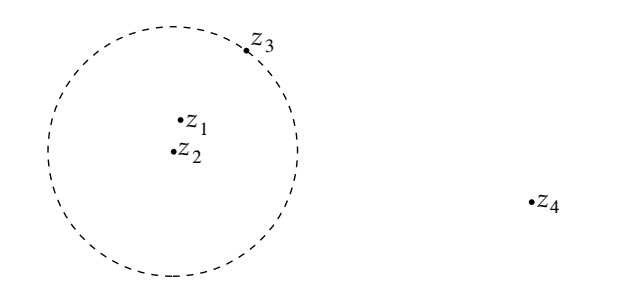
\includegraphics[width=0.8\textwidth,natwidth=400,natheight=180]{Fig2.1.jpg}\\
\caption{Expectation value of a product of four local operators. The OPE gives the asymptotics as $z_1 \to z_2$ as a series where the pair of operators at $z_1 $ and $ z_2$ is replaced by a single operator at $z_2$. The radius of convergence is the distance to	the nearest other operator, indicated by the dashed circle.}\label{Fig2.1}
	\end{center}
\end{figure}
上图是四个定域算符的乘积. OPE将$z_1 \to z_2$时渐近表示为一个级数. 其中$z_1 , z_2$一对算符被$z_2$处的单个算符代替. 收敛半径是到其他最近算符的距离.\\
OPE陈述为,两个彼此接近的定域算符的乘积可以以任意精度被定域算符的和近似:
\begin{equation}
\mathscr{A}_{i}\left(\sigma_{1}\right) \mathscr{A}_{j}\left(\sigma_{2}\right)=\sum_{k} c_{i j}^{k}\left(\sigma_{1}-\sigma_{2}\right) \mathscr{A}_{k}\left(\sigma_{2}\right)
\end{equation}
这是一个算符陈述,意味着其在一个普遍期望值中成立
\begin{equation}
\left\langle\mathscr{A}_{i}\left(\sigma_{1}\right) \mathscr{A}_{j}\left(\sigma_{2}\right) \ldots\right\rangle=\sum_{k} c_{i j}^{k}\left(\sigma_{1}-\sigma_{2}\right)\left\langle\mathscr{A}_{k}\left(\sigma_{2}\right) \ldots\right\rangle
\end{equation}
只要$\sigma_{1}$,$\sigma_{2}$之间的间隔小于与其他所有算符的距离.\\
系数函数 $c^{k}{ }_{i j}\left(\sigma_{1}-\sigma_{2}\right)$决定对间隔的依赖关系,其也依赖于i,j,k. 但与期望值中的其他算符无关. 后者的依赖性仅出现在(2.2.3)右边的期望值中. 这些项通常的排列方法是:$\sigma_{1} \rightarrow \sigma_{2}$的极限下,大小逐减. 这是对普通Taylor级数的类比. 除了系数函数不是简单的幂级数,并可以在$\sigma_{1} \rightarrow \sigma_{2}$时奇异.\\
我们现在将给出$X^\mu$理论的OPE推导. 其中利用了自由场论的特殊性质. 在2.9节将给出任意共形不变场论的推导. 我们已经看到,正规乘积满足运动方程(2.1.23). 这说明算符乘积是$\left(z_{1}, \bar{z}_{1}\right)$的调和函数. 复变函数论中一个简单的结果是,调和函数局域是一个全纯函数与一个反全纯函数之和. 尤其是,它意味着在$z_{1} \rightarrow z_{2}$时是不奇异的. 并且可以自由地以$z_{12}$ and $\bar{z}_{12}$ 做Taylor展开
\begin{equation}
\begin{array}{l}
X^{\mu}\left(z_{1}, \bar{z}_{1}\right) X^{v}\left(z_{2}, \bar{z}_{2}\right)=-\frac{\alpha^{\prime}}{2} \eta^{\mu \nu} \ln \left|z_{12}\right|^{2}+: X^{v} X^{\mu}\left(z_{2}, \bar{z}_{2}\right): \\
+\sum_{k=1}^{\infty} \frac{1}{k !}\left[\left(z_{12}\right)^{k}: X^{v} \partial^{k} X^{\mu}\left(z_{2}, \bar{z}_{2}\right):+\left(\bar{z}_{12}\right)^{k}: X^{v} \bar{\partial}^{k} X^{\mu}\left(z_{2}, \bar{z}_{2}\right):\right]
\end{array}
\end{equation}
\begin{remark}
$$\begin{aligned}
&:X^{\mu}\left(z_{1},  \bar{z}_{1}\right) X^{\nu}\left(z_{2}, \bar{z}_{2}\right):\\
=&: X^{\nu} X^{\mu}\left(z_{2}, \bar{z}_{2}\right):+\sum_{k=1}^{\infty} \frac{1}{k !}\left[\left(z_{12}\right)^{k}: X^{\nu} \partial^{k} X^{\mu}\left(z_{2}, \bar{z}_{2}\right):+\left(\bar{z}_{12}\right)^{k}:X^{\nu} \bar{\partial}^{k} X^{\mu}\left(z_{2}, \bar{z}_{2}\right):\right]
\end{aligned}
$$
倘若有定义
$$\partial_{1}:X^{\mu}\left(z_{1}, \bar{z}_{1}\right) X^{\nu}\left(z_{2}, \bar{z}_{2}\right):=: X^{\nu} \partial_{1}X^{\mu}:=X^{\nu} \partial_1 X^{\mu}+\frac{\alpha^{\prime}}{2} \eta^{\mu \nu} \partial_{1} \ln |z_{12}|^{2}$$
上式是可以解释的.
\end{remark}
------------------------------------------------------------------------------------------------------------
\\
Terms with mixed $\partial \bar{\partial}$ derivatives vanish by the equation of motion. This equation and many others simplify in units in which $\alpha^{\prime}=2$, which is the most common convention in the literature. However, several other conventions are also used, so it is useful to keep $\alpha^{\prime}$ explicit. For example, in open string theory equations simplify when $\alpha^{\prime}=\frac{1}{2}$.

Eq. (2.2.4) has the form of an OPE. Like the equation of motion ( $2.1 .23$ ) from which it was derived, it is an operator statement. For an arbitrary expectation value involving the product $X^{\mu}\left(z_{1}, \bar{z}_{1}\right) X^{v}\left(z_{2}, \bar{z}_{2}\right)$ times fields at other points, it gives the behavior for $z_{1} \rightarrow z_{2}$ as an infinite series, each term being a known function of $z_{12}$ and/or $\bar{z}_{12}$ times the expectation value with a local operator replacing the pair.

OPEs are usually used as asymptotic expansions, the first few terms
giving the dominant behavior at small separation. Most of our applications will be of this type, and we will often write OPEs as explicit singular
terms plus unspecified nonsingular remainders. The use of ‘∼’ in place of
‘=’ will mean ‘equal up to nonsingular terms.’ In fact, OPEs are actually
convergent in conformally invariant field theories. This will be very important to us in certain applications: it makes it possible to reconstruct
the entire theory from the coefficient functions. As an example, the freefield OPE (2.2.4) has a radius of convergence in any given expectation
value which is equal to the distance to the nearest other insertion in the
path integral. The operator product is harmonic except at the positions
of operators, and in particular inside the dashed circle of figure 2.1, and
convergence can then be shown by a standard argument from the theory
of complex variables.
The various operators on the right-hand side of the OPE (2.2.4) involve
products of fields at the same point. Usually in quantum field theory such
a product is divergent and must be appropriately cut off and renormalized,
but here the normal ordering renders it well-defined. Normal ordering is a
convenient way to define composite operators in free field theory. It is of
little use in most interacting field theories, because these have additional
divergences from interaction vertices approaching the composite operator
or one another. However, many of the field theories that we will be

interested in are free, and many others can be related to free field theories,
so it will be worthwhile to develop normal ordering somewhat further.
The definition of normal ordering for arbitrary numbers of fields can
be given recursively as
\begin{equation}
\begin{array}{l}
: X^{\mu_{1}}\left(z_{1}, \bar{z}_{1}\right) \ldots X^{\mu_{n}}\left(z_{n}, \bar{z}_{n}\right): \\
\quad=X^{\mu_{1}}\left(z_{1}, \bar{z}_{1}\right) \ldots X^{\mu_{n}}\left(z_{n}, \bar{z}_{n}\right)+\sum \text { subtractions }
\end{array}
\end{equation}
where the sum runs over all ways of choosing one, two, or more pairs of fields from the product and replacing each pair with $\frac{1}{2} \alpha^{\prime} \eta^{\mu_{i} \mu_{j}} \ln \left|z_{i j}\right|^{2}$. For example,\begin{equation}
\begin{array}{l}
: X^{\mu_{1}}\left(z_{1}, \bar{z}_{1}\right) X^{\mu_{2}}\left(z_{2}, \bar{z}_{2}\right) X^{\mu_{3}}\left(z_{3}, \bar{z}_{3}\right):=X^{\mu_{1}}\left(z_{1}, \bar{z}_{1}\right) X^{\mu_{2}}\left(z_{2}, \bar{z}_{2}\right) X^{\mu_{3}}\left(z_{3}, \bar{z}_{3}\right) \\
\quad+\left(\frac{\alpha^{\prime}}{2} \eta^{\mu_{1} \mu_{2}} \ln \left|z_{12}\right|^{2} X^{\mu_{3}}\left(z_{3}, \bar{z}_{3}\right)+2 \text { permutations }\right)
\end{array}
\end{equation}
We leave it to the reader to show that the definition (2.2.5) retains the desired property that the normal ordered product satisfies the naive equation
of motion.
The definition can be compactly summarized as
\begin{equation}
: \mathscr{F}:=\exp \left(\frac{\alpha^{\prime}}{4} \int d^{2} z_{1} d^{2} z_{2} \ln \left|z_{12}\right|^{2} \frac{\delta}{\delta X^{\mu}\left(z_{1}, \bar{z}_{1}\right)} \frac{\delta}{\delta X_{\mu}\left(z_{2}, \bar{z}_{2}\right)}\right) \mathscr{F}
\end{equation}
where $\mathscr{F}$ is any functional of $X .$ This is equivalent to eq. $(2.2 .5):$ the double derivative in the exponent contracts each pair of fields, and the exponential sums over any number of pairs with the factorial canceling the number of ways the derivatives can act. As an example of the use of this formal expression, act on both sides with the inverse exponential to obtain
\begin{equation}
\begin{aligned}
\mathscr{F} &=\exp \left(-\frac{\alpha^{\prime}}{4} \int d^{2} z_{1} d^{2} z_{2} \ln \left|z_{12}\right|^{2} \frac{\delta}{\delta X^{\mu}\left(z_{1}, \bar{z}_{1}\right)} \frac{\delta}{\delta X_{\mu}\left(z_{2}, \bar{z}_{2}\right)}\right): \mathscr{F}: \\
&=: \mathscr{F}:+\sum \text { contractions }
\end{aligned}
\end{equation}
where a contraction is the opposite of a subtraction: sum over all ways of choosing one, two, or more pairs of fields from $: \mathscr{F}:$ and replacing each pair with $-\frac{1}{2} \alpha^{\prime} \eta^{\mu_{i} \mu_{j}} \ln \left|z_{i j}\right|^{2}$.
The OPE for any pair of operators can be generated from
\begin{equation}
: \mathscr{F}:: \mathscr{G}:=: \mathscr{F} \mathscr{G}:+\sum \text { cross-contractions }
\end{equation}
for arbitrary functionals $\mathscr{F}$ and $\mathscr{G}$ of $X$. The sum now runs over all ways of contracting pairs with one field in $\mathscr{F}$ and one in $\mathscr{G} .$ This can also be written
\begin{equation}
: \mathscr{F}:: \mathscr{G}:=\exp \left(-\frac{\alpha^{\prime}}{2} \int d^{2} z_{1} d^{2} z_{2} \ln \left|z_{12}\right|^{2} \frac{\delta}{\delta X_{F}^{\mu}\left(z_{1}, \bar{z}_{1}\right)} \frac{\delta}{\delta X_{G \mu}\left(z_{2}, \bar{z}_{2}\right)}\right): \mathscr{F} \mathscr{G}:
\end{equation}
where the functional derivatives act only on the fields in $\mathscr{F}$ or $\mathscr{G}$ respectively. This follows readily from eq. (2.2.7). As an example,
\begin{equation}\label{2.2.11}
\begin{aligned}
&: \partial X^{\mu}(z) \partial X_{\mu}(z):: \partial^{\prime} X^{v}\left(z^{\prime}\right) \partial^{\prime} X_{v}\left(z^{\prime}\right): \\
=&: \partial X^{\mu}(z) \partial X_{\mu}(z) \partial^{\prime} X^{v}\left(z^{\prime}\right) \partial^{\prime} X_{v}\left(z^{\prime}\right): \\
&-4 \cdot \frac{\alpha^{\prime}}{2}\left(\partial \partial^{\prime} \ln \left|z-z^{\prime}\right|^{2}\right): \partial X^{\mu}(z) \partial^{\prime} X_{\mu}\left(z^{\prime}\right): \\
&+2 \cdot \eta^{\mu}{ }_{\mu}\left(-\frac{\alpha^{\prime}}{2} \partial \partial^{\prime} \ln \left|z-z^{\prime}\right|^{2}\right)^{2} \\
\sim &\frac{D \alpha^{\prime 2}}{2\left(z-z^{\prime}\right)^{4}}-\frac{2 \alpha^{\prime}}{\left(z-z^{\prime}\right)^{2}}: \partial^{\prime} X^{\mu}\left(z^{\prime}\right) \partial^{\prime} X_{\mu}\left(z^{\prime}\right): \\
&-\frac{2 \alpha^{\prime}}{z-z^{\prime}}: \partial^{\prime 2} X^{\mu}\left(z^{\prime}\right) \partial^{\prime} X_{\mu}\left(z^{\prime}\right):
\end{aligned}
\end{equation}
The second term in the equality comes from the four ways of forming a single pair and the third from the two ways of forming two pairs. In the final line we have put the OPE in standard form by Taylor expanding inside the normal ordering to express everything in terms of local operators at $z^{\prime}$ and putting the most singular terms first. \\
%$\underbracket{XYZUVW}$
%$\contraction{A}{B}{C}{D}ABCD$

\begin{remark}
$$
\begin{aligned}
&\contraction{: \partial}{X^{\mu}}{(z) \partial X_{\mu}(z):: \partial^{\prime}}{X^{\nu}}
: \partial  X^{\mu}(z) \partial X_{\mu}(z):: \partial^{\prime} X^{\nu} \left(z^{\prime}\right) \partial^{\prime} X_{\nu}\left(z^{\prime}\right):\\ =&\partial \partial^{\prime}\left(-\frac{\alpha^{\prime}}{2} \eta^{\mu \nu}|n| z-\left.z^{\prime}\right|^{2}\right): \partial X_{\mu}(z) \partial X_{\nu}(z):\\
=&-\left(\partial \partial^{\prime} \ln \left|z-z^{\prime}\right|^{2}\right) \cdot \frac{\alpha^{\prime}}{2}: \partial X_{\mu}(z) \partial^{\prime} X^{\mu}(z):
\end{aligned}
$$

$$
\begin{aligned}
&\contraction[2ex]{: \partial}{X^{\mu}}{(z) \partial X_{\mu}(z):: \partial^{\prime}}{X^{\nu}}
\bcontraction{: \partial X^\mu(z) \partial}{ X_\mu}{(z):: \partial^\prime X^\nu(z^\prime)\partial^\prime}{X_\nu}
	: \partial X^{\mu}(z) \partial X_{\mu}(z):: \partial^{\prime} X^{\nu}\left(z^{\prime}\right) \partial^{\prime} X_{\nu}\left(z^{\prime}\right):\\
=&\partial \partial^{\prime}\left(-\frac{\alpha^{\prime}}{2} \eta ^{\mu \nu} \ln \left|z-z^{\prime}\right|^{2}\right) \partial \partial^{\prime}\left(-\frac{\alpha^{\prime}}{2} \eta^{\mu \nu}\ln \left|z-z^{\prime}\right|^{2}\right) \\
=&\eta^{\mu \nu} \eta_{\mu \nu}\left(-\frac{\alpha^{\prime}}{2} \partial \partial^{\prime}\ln | z-\left.z^{\prime}\right|^{2}\right)^{2}
\end{aligned}
$$
而
$\eta^{\mu \nu} \eta_{\nu\rho}=\delta^{\mu}{ }_{p}, \quad \eta^{\mu \nu} \eta_{\mu \nu}=\delta^{\mu}{ }_{\mu}=D$,
且
$$
(1)=2 \cdot \eta^{\mu}{ }_{\mu}\left(-\frac{\alpha^{\prime}}{2} \frac{1}{\left(z-z^{\prime}\right)^{2}}\right)^{2}=2 D \cdot \frac{\alpha^{\prime 2}}{4} \frac{1}{\left(z-z^{\prime}\right)^{4}}=\frac{D \alpha^{\prime 2}}{2\left(z-z^{\prime}\right)^{4}}
$$

$$
(2)=\partial \partial^{\prime} \ln \left|z-z^{\prime 2}\right|^{2}=\partial \partial^{\prime}\left(\ln \left(z-z^{\prime}\right)+\ln \left(\bar{z}+\bar{z}^{\prime}\right)=\partial^{\prime} \frac{1}{z-z^{\prime}}=+\frac{1}{\left(z^{\prime}-z\right)^{2}}\right.
$$

$$
(3)=:\partial X^\mu(z)\partial^\prime X_{\mu}(z^\prime):\sim \partial^\prime X^\mu(z^\prime)\partial^\prime X_\mu(z^\prime): +(z-z^\prime):\partial^{\prime 2} X^\mu(z^\prime)\partial^\prime X_\mu(z):
$$
于是
$$
: \partial X^{\mu}(z) \partial X_{\mu}(z):: \partial^{\prime} X^{\nu}\left(z^{\prime}\right) \partial^{\prime} X_{\nu}\left(z^{\prime}\right):  \sim (1)+(2)\cdot(3)
$$
\end{remark}
Another important example is
\begin{equation}
\mathscr{F}=e^{i k_{1} \cdot X(z, \bar{z})}, \quad \mathscr{G}=e^{i k_{2} \cdot X(0,0)}
\end{equation}
The variations $\delta / \delta X_{F}^{\mu}$ and $\delta / \delta X_{G}^{\mu}$ give factors of $i k_{1 \mu}$ and $i k_{2 \mu}$ respectively, so the general result $(2.2 .10)$ becomes
\begin{equation}\label{2.2.13}
\begin{aligned}
: e^{i k_{1} \cdot X(z, \bar{z})}:: e^{i k_{2} \cdot X(0,0)}: &=\exp \left(\frac{\alpha^{\prime}}{2} k_{1} \cdot k_{2} \ln |z|^{2}\right): e^{i k_{1} \cdot X(z, \bar{z})} e^{i k_{2} \cdot X(0,0)} :\\
&=|z|^{\alpha^{\prime} k_{1} \cdot k_{2}}: e^{i k_{1} \cdot X(z, \bar{z})} e^{i k_{2} \cdot X(0,0)}:
\end{aligned}
\end{equation}

\begin{remark}
$$
\begin{aligned}
&:e^{i k_{1} \cdot x(z, z)}:: e^{i k_{2} \cdot x(0.0)}:\\
=&\exp \left(-\frac{\alpha^{\prime}}{2} \int d^{2} z_{1} d^{2} z_{2} \ln \left|z_{12}\right|^{2} \frac{\delta}{\delta X_{F}^{\mu}\left(z_{1}, \bar{z}_{1}\right)} \frac{\delta}{\delta X_{G\mu}\left(z_{2}, \bar{z}_{2}\right)}\right): e^{i k_{1} \cdot x(z, \bar{z})} e^{i k_{2} \cdot x(0,0)}:\\
=&\left(1-\frac{\alpha^{\prime}}{2} \int d^{2} z_{1} d^{2} z_{2} \ln \left|z_{12}\right|^{2} \frac{\delta}{\delta X_{F}^{\mu}\left(z_{1}, z_{1}\right)} \frac{\delta}{\delta X_{G \mu}\left(z_{2}, \bar{z}_{2}\right)} \right): e^{i k_{1} \cdot x(z, \bar{z})} e^{i k_{2} \cdot x(0,0)}:+\cdots\\
=&: e^{i k_{1} \cdot x(z, \bar{z})} e^{i k_{2} \cdot x(0,0)}-\frac{\alpha^{\prime}}{2} \int d^{2} z_{1} d^{2} z_{2} \ln \left|z_{12}\right|^{2}
:e^{i k_{1} \cdot x\left(z, \bar{z}\right)} e^{i k_{2} \cdot x ( 0,0)}:\\
&\qquad \qquad \qquad \qquad \qquad
 \times i k_{1 \mu} \delta\left(z-z_{1}, \bar{z}-\bar{z}_{1}\right) i k_{2}^{\mu} \delta\left(0-z_{2}, 0,-\bar{z}_{2}\right)\\
=&e^{i k_{1} \cdot x(z, \bar{z})} e^{i k_{2} \cdot x(0,0)}:\left(1+\frac{\alpha^{\prime}}{2} k_{1} \cdot k_{2} \ln |z|^{2}+\cdots\right)
\end{aligned}
$$
\end{remark}

To derive the OPE, Taylor expand inside the normal ordering to give
\begin{equation}
: e^{i k_{1} \cdot X(z, \bar{z})}:: e^{i k_{2} \cdot X(0,0)}:=|z|^{\alpha^{\prime} k_{1} \cdot k_{2}}: e^{i\left(k_{1}+k_{2}\right) \cdot X(0,0)}[1+O(z, \bar{z})]:
\end{equation}
The exercises give further practice with normal ordering and the free-field OPE.

Note that the OPEs (2.2.2), (2.2.4), and so on have been written asymmetrically in $\sigma_{1}$ and $\sigma_{2}$, expanding around the latter point. They can also be cast in symmetric form by Taylor expanding the right-hand sides around $\left(\sigma_{1}+\sigma_{2}\right) / 2$. The coefficient functions for the symmetric form behave simply under interchange of the two operators,
\begin{equation}
c_{i j}^{k}\left(\sigma_{1}-\sigma_{2}\right)_{\mathrm{sym}}=\pm c_{j i}^{k}\left(\sigma_{2}-\sigma_{1}\right)_{\mathrm{sym}}
\end{equation}
where the minus sign appears if $\mathscr{A}_{i}$ and $\mathscr{A}_{j}$ are both anticommuting. The asymmetric form is usually more convenient for calculation, so when the
symmetry properties of the coefficient functions are needed one can work
them out in the symmetric form and then convert to the asymmetric form.

\section{Ward恒等式}%{2.3 Ward identities and Noether theorem}
世界面对称性在弦论中扮演了一个重要角色. 在本节,我们先导出场论中对称性的一些普遍结果.\\
考察一个场论,作用量为$S_\phi$. 在d维时空中,$\phi_\alpha(\sigma)$标记一般场. 让它存在对称性
\begin{equation}
\phi_{\alpha}^{\prime}(\sigma)=\phi_{\alpha}(\sigma)+\delta \phi_{\alpha}(\sigma)
\end{equation}
其中$\delta \phi_\alpha$正比于无限小参量$\epsilon$. 路径积分测度与权重$exp(-S)$之积是不变的:
\begin{equation}
\left[d \phi^{\prime}\right] \exp \left(-S\left[\phi^{\prime}\right]\right)=[d \phi] \exp (-S[\phi])
\end{equation}
场论中,连续对称性暗示着守恒流的存在(Noether定理),以及Ward等式(其约束流的算符积). 为了导出这些结果,考察变量的改变
\begin{equation}\label{2.3.3}
\phi_{\alpha}^{\prime}(\sigma)=\phi_{\alpha}(\sigma)+\rho(\sigma) \delta \phi_{\alpha}(\sigma)
\end{equation}
这不是对称性,$[\dif \phi]\mathrm{exp}(-S)$在$\rho$是一常量下不变,所以它的变分必须正比于$\partial _a \rho$
\begin{equation}
\begin{array}{l}
{\left[d \phi^{\prime}\right] \exp \left(-S\left[\phi^{\prime}\right]\right)} \\
\quad=[d \phi] \exp (-S[\phi])\left[1+\frac{i \epsilon}{2 \pi} \int d^{d} \sigma g^{1 / 2} j^{a}(\sigma) \partial_{a} \rho(\sigma)+O\left(\epsilon^{2}\right)\right]
\end{array}
\end{equation}
未知系数$j^a(\sigma)$源于测度和作用量的变分,仅在一个小区域里取$\rho$非零. 在区域之外,考察一个普遍插入$'\cdots'$ 的路径积分。这个插入(\ref{2.3.3}) 下不变:
\begin{equation}
\begin{aligned}
0 &=\int\left[d \phi^{\prime}\right] \exp \left(-S\left[\phi^{\prime}\right]\right) \ldots-\int[d \phi] \exp (-S[\phi]) \ldots \\
&=\frac{\epsilon}{2 \pi i} \int d^{d} \sigma g^{1 / 2} \rho(\sigma)\left\langle\nabla_{a} j^{a}(\sigma) \ldots\right\rangle
\end{aligned}
\end{equation}
因而我们有
\begin{equation}
\nabla_{a} j^{a}=0
\end{equation}

\begin{remark}
(2.3.4)的补充说明:
$$
\frac{i \epsilon}{2 \pi} \int d ^d \sigma g^{1 / 2} j^{a}(\sigma) \partial_{a} \rho(\sigma) 
=\frac{\epsilon}{2 \pi i} \int d^{d} \sigma \partial_{a}\left(g^{1 / 2}j^{a}\right)\rho(\sigma)
$$
$$
\partial_{a}\left(g^{1 / 2} j^{a}\right)=\partial_{a} j^{a} \cdot g^{1 / 2}+j^{a} \partial_{a} g^{1 / 2}
=g^{1 / 2}\nabla_{a}j^{a}
$$
\end{remark}
为了导出ward等式,令$\rho(\sigma)$在区域R内为1,在R外为0. 另外在路径积分中引入一般定域算符$\mathscr{A}\left(\sigma_{0}\right)$. $\sigma_0$在R内. 在R外引入$'\cdots'$得到
\begin{equation}
\delta \mathscr{A}\left(\sigma_{0}\right)+\frac{\epsilon}{2 \pi i} \int_{R} d^{d} \sigma g^{1 / 2} \nabla_{a} j^{a}(\sigma) \mathscr{A}\left(\sigma_{0}\right)=0
\end{equation}

\begin{proof}
关于(2.3.7)的证明:
由(2.3.4)
$$
\delta \exp \left(-S\left[\phi^{\prime}\right]\right)=\frac{ \epsilon}{2 \pi i} \int d^{d} \sigma g^{1 / 2} \nabla_{a} j^{a}(\sigma) \rho(\sigma) \cdot e^{-S}
$$
$$
\delta\left[\exp (-S[\phi]) \mathscr{A}\left(\sigma_{0}\right)\right]=\delta e^{-S} \mathscr{A}\left(\sigma_{0}\right)+e^{-S} \delta\mathscr{A}(\sigma_0)=0
$$
$$
\delta \mathscr{A}\left(\sigma_{0}\right) +\mathscr{A}\left(\sigma_{0}\right) e^{S} \delta e^{-S}=0
$$
$$
\delta \mathscr{A}\left(\sigma_{0}\right)+\frac{\sigma}{2 \pi i} \int_{R} d^{d} \sigma g^{1 / 2} \nabla_{a} j^{a}(\sigma) \mathscr{A}\left(\sigma_{0}\right)=0
$$
而
$$
\int_{R} d^{d} \sigma g^{1 / 2} \nabla_{a} j^{a} =\int_{R} d^{d} \sigma \partial_{a}\left(g^{1 / 2} j^{a}\right) 
=\int_{\partial R} d A n_{\alpha} j^{a}
$$
在复坐标下
$$
\int_{R} d^{2} z\left(\partial_{z} v^{z}+\partial_{\bar{z}} v^{\bar{z}}\right)=i \oint_{\partial R}(v^{z} d \bar{z}-v^{\bar{z}} d \bar{z})
$$
$$
\int g^{1 / 2} \nabla_{a} j^{a}=\int\left(\partial_{z} j^{z}+\partial_{\bar{z}} j^{\bar{z}}\right)\frac{1}{2}=\int 2\left(\partial_{z} j_{\bar{z}}+\partial_{z} j_{z}\right) \frac{1}{2}
$$
\end{proof}

等价地,
\begin{equation}
\nabla_{a} j^{a}(\sigma) \mathscr{A}\left(\sigma_{0}\right)=g^{-1 / 2} \delta^{d}\left(\sigma-\sigma_{0}\right) \frac{2 \pi}{i \epsilon} \delta \mathscr{A}\left(\sigma_{0}\right)+\text { total } \sigma \text { -derivative }
\end{equation}
散度定理给出
\begin{equation}
\int_{\partial R} d A n_{a} j^{a} \mathscr{A}\left(\sigma_{0}\right)=\frac{2 \pi}{i \epsilon} \delta \mathscr{A}\left(\sigma_{0}\right)
\end{equation}
在2维平坦空间中
\begin{equation}
\oint_{\partial R}(j d z-\tilde{\jmath} d \bar{z}) \mathscr{A}\left(z_{0}, \bar{z}_{0}\right)=\frac{2 \pi}{\epsilon} \delta \mathscr{A}\left(z_{0}, \bar{z}_{0}\right)
\end{equation}
在这里我们扔掉了指标$j \equiv j_{z}, \tilde{\jmath} \equiv j_{\bar{z}}$. 我们使用$\tilde{j}$而非$\bar{j}$是因为$\tilde{j}$并非j的共轭. Minkowski密度$j_0$一般是Hermitean的,$\left(j_{z}\right)^{\dagger}=\frac{1}{2}\left(j_{1}-i j_{2}\right)^{\dagger}=j_{z}$.\\
重要的是Noether定理和Ward等式是定域性质,并不依赖于远处的边界条件,也不依赖在对称下是否不变. 特别的,因为$\rho(\sigma)$仅在R内非零,仅需要在这里定义对称变换.\\
在共形不变理论中,通常$j_z$是全纯的,而$j_{\bar{z}}$是反全纯的. 在这种情况下,流$(j_z,0),(0,j_{\bar{z}})$分别守恒. 于是积分给出OPE中的留数:
\begin{equation}\label{2.3.11}
\operatorname{Res}_{z \rightarrow z_{0}} j(z) \mathscr{A}\left(z_{0}, \bar{z}_{0}\right)+\overline{\operatorname{Res}}_{\bar{z} \rightarrow \bar{z}_{0}} \tilde{J}(\bar{z}) \mathscr{A}\left(z_{0}, \bar{z}_{0}\right)=\frac{1}{i \epsilon} \delta \mathscr{A}\left(z_{0}, \bar{z}_{0}\right)
\end{equation}
这里$\mathrm{Res},\mathrm{\bar{Res}}$分别是$\left(z-z_{0}\right)^{-1}, \left(\bar{z}-\bar{z}_{0}\right)^{-1}$的系数.\\
一个例子:无质量自由标量场\\
考虑时空平移$\delta X^{\mu}=\epsilon a^{\mu}$. 在$\delta X^{\mu}(\sigma)=\epsilon \rho(\sigma) a^{\mu}$ 下,
\begin{equation}
\begin{aligned}
\delta S&=\frac{1}{4 \pi \alpha^{\prime}} \int d^{2} \pm 2 \delta \partial^{a} X^{\mu} \partial_{a} X_{\mu}\\
&=-\frac{1}{2\pi \alpha^{\prime}} \int d^{2} z \delta X^{\mu} \partial^{a} \partial_{a} X_{\mu} \\
&=-\frac{1}{2 \pi \alpha^{\prime}} \int d^{2} z \quad \epsilon p(\sigma) a^{\mu} \partial^{a} \partial_{a} X_{\mu}\\
&=\frac{\epsilon a_{\mu}}{2 \pi \alpha^{\prime}} \int d^{2} \sigma \partial^{a} X^{\mu} \partial_{a} \rho
\end{aligned}
\end{equation}
令$\delta S=\frac{i \epsilon}{2 \pi \alpha^\prime} \int d^{2} z \, j^{a}(\sigma)  \partial _a \rho$,则
$j_{a}(\sigma)=a_{\mu} j_{a}^{\mu}$
\begin{equation}
j_{a}^{\mu}=\frac{i}{\alpha^{\prime}} \partial_{a} X^{\mu}
\end{equation}
并且
\begin{subequations}
\begin{equation}
j^{\mu}(z): e^{i k \cdot X(0,0)}: \sim \frac{k^{\mu}}{2 z}: e^{i k \cdot X(0,0)}:
\end{equation}
\begin{equation}
\tilde{\jmath}^{\mu}(\bar{z}): e^{i k \cdot X(0,0)}: \sim \frac{k^{\mu}}{2 \bar{z}}: e^{i k \cdot X(0,0)}:
\end{equation}
\end{subequations}

\begin{proof}
(2.3.14a)的说明:
由(2.3.13)
$$
j^{\mu}=j_{z}^{\mu}=\frac{i}{\alpha^{\prime}} \partial_{z} X^{\mu}
$$
$$
\begin{aligned}
& \frac{i}{\alpha^{\prime}}: \partial_{z}X^{\mu}: : e^{i k \cdot x(0,0)}: \\
=& \frac{i}{\alpha^{\prime}} \exp \left(-\frac{\alpha^{\prime}}{2} \int d^{2} z_{1} d^{2} z_{2} \ln \left|z_{12}\right|^{2} \frac{\delta}{\delta X_{F}^{\mu}\left(z_{1}, \bar{z}_{1}\right)} \frac{\delta}{\delta X_{G{\mu}}\left(z_{2}, \bar{z}_{2}\right)}\right): \partial_{z}X^{\mu} e^{i k \cdot x(0,0)}: \\
=& \frac{i}{\alpha^{\prime}}\left(1-\frac{\alpha^{\prime}}{2} \int d^{2} z_{1} d^{2} z_{2} \ln \left|z_{12}\right|^{2} \frac{\delta}{\delta X^{\mu}} \frac{\delta}{\delta X_{u}}-\cdots\right) : \partial_{z} X^{\mu} e^{i k \cdot x}:\\
=&\frac{i}{\alpha^{\prime}}: \partial_{z} X^{\mu} e^{i k  x(0,0)}:-\frac{i}{2} \partial_{z} \int d^{2} z_{1} d^{2} z_{2} \ln \left|z_{12}\right|^{2} \delta\left(z-z_{1}, \bar{z}-\bar{z}_{1}\right)  i k_{2}^{\mu} \delta\left(-z_{2}, -\bar{z}_{2}\right):e^{ikx}:\\
\sim&-\frac{i}{2} \partial_{z} \ln |z|^{2} \cdot i k^{\mu}: e^{i k \cdot x(0,0)}: \\
=&\frac{1}{2} \frac{1}{z} i k^{\mu}: e^{i k \cdot x(0,0)}:=\frac{i k^{\mu}}{2 z}: e^{i k \cdot x(0,0)}:
\end{aligned}
$$
\end{proof}

另一例子:世界面平移$\delta \sigma^{a}=\epsilon v^{a}$\\
这时$\delta X^{\mu}=-\epsilon v^{a} \partial_{a} X^{\mu}$,Noether流
\begin{subequations}
\begin{equation}\label{2.3.15a}
j_{a}=i v^{b} T_{a b}
\end{equation}
\begin{equation}
T_{a b}=-\frac{1}{\alpha^{\prime}}:\left(\partial_{a} X^{\mu} \partial_{b} X_{\mu}-\frac{1}{2} \delta_{a b} \partial_{c} X^{\mu} \partial^{c} X_{\mu}\right):
\end{equation}
\end{subequations}

\begin{proof}
(2.3.15a)的证明:
$$
\delta \sigma^{u}=\epsilon v^{a}, \quad \delta X^{\mu}=-\partial_{a} X^{\mu} \delta \sigma^{a}=-\epsilon v^{a} \partial_{a} X^{\mu}
$$
$$
\begin{aligned}
\delta S &=\frac{1}{4 \pi \alpha^{\prime}} \int d^{2} \sigma 2 \delta \partial^{\alpha} X^{\mu} \partial_{a} X_{\mu} \\
&=-\frac{1}{2 \pi \alpha^{\prime}} \int d^{2} \sigma \delta X^{\mu} \partial^{a} \partial_{a} X_{\mu} \\
&=-\frac{1}{2 \pi \alpha^{\prime}} \int d^{2} \sigma\left(-\epsilon v^{a} \partial_{\alpha} X^{\mu}\right) \rho(\sigma) \partial^{\alpha} \partial_{a} X_{\mu} \\
&=\frac{\epsilon v^{\alpha}}{2 \pi \alpha^{\prime}} \int d^{2} \sigma  \partial_{a} X^{\mu} \rho(\sigma) \partial^{b} \partial_{b} X_{u}
\end{aligned}
$$
$$
\begin{array}{l}
\int d^{2} \sigma \partial_{b}\left(\partial_{a} X^{\mu} \rho(\sigma)\right) \partial^{b} X_{u} \\
=\int d^{2} \sigma  \partial_{a} X^{\mu} \partial^{b} X_{\mu} \partial_{b} \rho(\sigma)+\rho(\sigma) \partial_{b} \partial_{a} X^{\mu} \partial^{b} X_{\mu}\\
=\int d^{2} \sigma \partial_{a} X^{\mu} \partial^{b} X_{\mu} \partial_{b} \rho(\sigma)-\partial_{a} \rho(\sigma) \partial_{b} X^{\mu} \partial^{b} X_{\mu}-\rho(\sigma) \partial_{a} X^{\mu} \partial_{b} \partial^{b} X^{\mu} \\
=\int d^{2} \sigma \partial_{a} X^{\mu} \rho(\sigma) \partial^{b} \partial_{b} X^{\mu} \\
=\frac{1}{2} \int d^{2} \sigma \partial_{a} X^{\mu} \partial^{b} X_{\mu} \partial_{b} \rho(\sigma)-\partial_{a} \rho(\sigma) \partial_{b} X^{\mu} \partial^{b} X_{u}
\end{array}
$$
$$
\frac{\epsilon v^{a}}{2 \pi \alpha^{\prime}} \int d^{2} \sigma \frac{1}{2} \left[\partial_{a} X^{\mu} \partial^{b} X_{\mu} \partial_{b} \rho(\sigma)-\partial_{a}\rho \partial_{b} X^{\mu}  \partial^{b} X_{\mu}\right]=\frac{i \epsilon}{2 \pi} \int d^{2} z j^{a}(\sigma) \partial_{a}(\rho)
$$
\end{proof}


\section{共形不变性}%{2.4 Conformal invariance}

能动量张量(\ref{2.3.15a})是无迹的,${T_a} ^a=0$. 在复坐标中,则是
\begin{equation}
T_{z \bar{z}}=0
\end{equation}
守恒律$\partial^a T_{ab}=0$暗示着在任何${T_a} ^a=0$的理论中
\begin{equation}
\bar{\partial} T_{z z}=\partial T_{\bar{z} \bar{z}}=0
\end{equation}
因此
\begin{equation}
T(z) \equiv T_{z z}(z), \quad \tilde{T}(\bar{z}) \equiv T_{\bar{z} \bar{z}}(\bar{z})
\end{equation}
分别是全纯的和反全纯的. 对于无质量自由标量
\begin{equation}\label{2.4.4}
T(z)=-\frac{1}{\alpha^{\prime}}: \partial X^{\mu} \partial X_{\mu}:, \quad \tilde{T}(\bar{z})=-\frac{1}{\alpha^{\prime}}: \bar{\partial} X^{\mu} \bar{\partial} X_{\mu}:
\end{equation}
作为运动方程的结果,其确实是全纯和反全纯的.\\
$T_{ab}$的无迹暗示着一个大得多的对称性. 流
\begin{equation}
j(z)=i v(z) T(z), \quad \tilde{\jmath}(\bar{z})=i v(z)^{*} \tilde{T}(\bar{z})
\end{equation}
对于全纯的$v(z)$是守恒的.
\begin{proof}
$$
j_{z}=i v^{z} T_{z z}, \quad j_{\bar{z}}=i v^{\bar{z}} T_{\bar{z} \bar{z}}
$$
由(2.1.5)
$$
v^{z}={v^{\bar{z}}}^*
$$
而
$$
\nabla_{a} j^{a}= \bar{\partial} j_{z}+\partial j_{\bar{z}}=0
$$
所以$v^z$为全纯.
\end{proof}
对于自由标量理论,得到OPE
\begin{equation}
T(z) X^{\mu}(0) \sim \frac{1}{z} \partial X^{\mu}(0), \quad \tilde{T}(\bar{z}) X^{\mu}(0) \sim \frac{1}{\bar{z}} \bar{\partial} X^{\mu}(0)
\end{equation}
\begin{proof}
$$
T(z)=-\frac{1}{\alpha^{\prime}}: \partial X^{\mu} \partial X_{\mu}:
$$
$$
-\frac{1}{\alpha^{\prime}}: \partial X^{\mu} \partial X_{\mu}: X^{\nu}(0)=-\frac{1}{\alpha^{\prime}}: \partial X^{\mu} \partial X_{\mu}(z) X^{\nu}(0):\sim \frac{1}{z} \partial X_{\mu} (0)
$$
\end{proof}
那么Ward等式给出变换
\begin{equation}\label{2.4.7}
\delta X^{\mu}=-\epsilon v(z) \partial X^{\mu}-\epsilon v(z)^{*} \bar{\partial} X^{\mu}
\end{equation}
\begin{proof}
由(\ref{2.3.11})
$$
\frac{1}{i \epsilon} \delta X^{\mu}=\operatorname{Res}_{z \rightarrow z_{0}^{\prime}} i v^{z} T_{z z} X^{\mu}+\overline{\operatorname{Res}}_{z \rightarrow z_{0}} i v^{\bar{z}} T_{\bar{z} \bar{z}} X^{\mu}
$$
前者$=i v^{z} \frac{1}{z-z_0} \partial X^{\mu}\left(z_{0}\right)$,
后者$=i v^{z *} \frac{1}{z} \bar{\partial} X^{\mu}\left(z_{0}\right)$
$$
\delta X^{\mu}=-\epsilon v^{z} \partial X^{\mu}\left(z_{0}\right)-\epsilon v^{\bar{z}} \bar{\partial} X^{\mu}\left(\bar{z}_{0}\right)
$$
\end{proof}
这是无限小坐标变换$z^{\prime}=z+\epsilon v(z)$. 
有限变换
\begin{equation}
X^{\prime \mu}\left(z^{\prime}, \bar{z}^{\prime}\right)=X^{\mu}(z, \bar{z}), \quad z^{\prime}=f(z)
\end{equation}
这是共形变换.
共形不变不应与diff不变相混淆. 我们处在平坦空间中,没有独立的度规场以供变化. 所以变换$z\to z^\prime$真的改变了内点的距离. 我们不是随随便便就有了这种不变性,它是关于动力学的非平庸陈述. 对于标量作用量(2.1.10),$\partial,\bar{\partial}$的共形变换与$d^2 z$的共形变换恰好抵消,质量项$m^{2} X^{\mu} X_{\mu}$将是不变的.
最终,存在一个与Polyakov弦的$diff\times Weyl$对称性的紧密联系. \\
考察特殊情况
\begin{equation}\label{2.4.9}
z^{\prime}=\zeta z
\end{equation}
$\zeta$为任意复数. $\zeta$的相位是系统的旋转,它的大小则是系统尺寸的重新标度. 这种标度不变性通常视为粒子物理中的一个近似对称性以及被标度不变场论描述的统计系统在临界点附近所拥有的近似对称性. \\
对于广义共形变换,考察$d s^{2}=d \sigma^{a} d \sigma^{a}=d z d \bar{z}$ 上的效应
\begin{equation}
d s^{\prime 2}=d z^{\prime} d \bar{z}^{\prime}=\frac{\partial z^{\prime}}{\partial z} \frac{\partial \bar{z}^{\prime}}{\partial \bar{z}} d z d \bar{z}
\end{equation}
我们看到共形变换将无限小平方变为无限小平方并调节了大小. 一个反全纯函数$z^{\prime}=f(z)^{*}$ 有相同的性质但改变了方向. \\
在(\ref{2.4.9})下不变的大多数系统通常在大得多的共形不变性不变. 有这种不变性的理论称为共形场论(CFT). \\
\begin{figure}
	\begin{center}
		%	\includegraphics[width=0.8\textwidth,bb=0 0 803 312]{Fig2.3ClosedStringCoordinates.jpg}\\
		%1px=0.75pt
		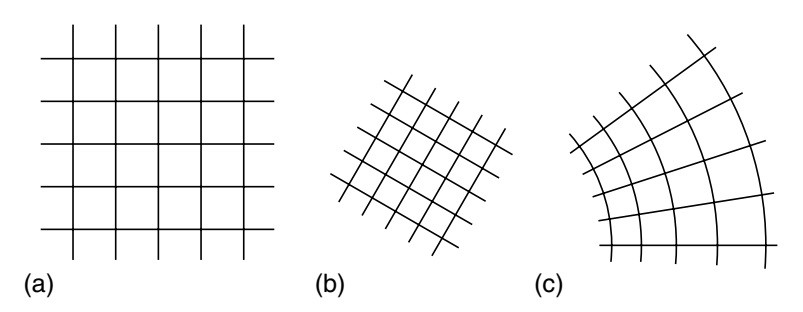
\includegraphics[width=0.8\textwidth,natwidth=520,natheight=200]{Fig2.2.jpg}\\
\caption{(a) Two-dimensional region. (b) Effect of the special conformal transformation (2.4.9). (c) Effect of a more general conformal transformation.}
	\end{center}
\end{figure}

\centerline{\Large 共形不变与OPE}
共形不变给OPE的形式施加了一个很强的约束,尤其是能动量张量的OPE. 考察T与一般算符$\mathscr{A}$的OPE. 因为$T(z)$和 $\tilde{T}(\bar{z})$除了交叉点以外是(反)全纯的,相应的系数函数也要有这个性质. T与$\mathscr{A}$的OPE因而是Laurent展开,是z的整数次但可能为负幂级数. 更进一步,所有项都由$\mathscr{A}$的共形变换决定. 为了看到这一点,我们写出一奇异性的普遍展开
\begin{equation}\label{2.4.11}
T(z) \mathscr{A}(0,0) \sim \sum_{n=0}^{\infty} \frac{1}{z^{n+1}} \mathscr{A}^{(n)}(0,0)
\end{equation}
与$\tilde{T}$相似,算符系数$\mathscr{A}^{(n)}$留到以后决定. 在无限小共形变换$z^{\prime}=z+\epsilon v(z)$下,当$T \mathscr{A}$ OPE中的$z^{-n-1}$ 项与$v(z)$中 $z^n$项相乘时,在$v(z) T(z) \mathscr{A}(0,0)$ 中会出现一个单极点. 
因此Ward等式的(\ref{2.3.11})形式暗示
\begin{equation}\label{2.4.12}
\delta \mathscr{A}(z, \bar{z})=-\epsilon \sum_{n=0}^{\infty} \frac{1}{n !}\left[\partial^{n} v(z) \mathscr{A}^{(n)}(z, \bar{z})+\bar{\partial}^{n} v(z)^{*} \tilde{\mathscr{A}}^{(n)}(z, \bar{z})\right]
\end{equation}
因此算符$\mathscr{A}^{(n)}$ 由$\mathscr{A}$的共形变换决定. 取在刚性变换(\ref{2.4.9})下为本征态的算符为基是方便的
\begin{equation}\label{2.4.13}
\mathscr{A}^{\prime}\left(z^{\prime}, \bar{z}^{\prime}\right)=\zeta^{-h \bar{\zeta}-\tilde{h}} \mathscr{A}(z, \bar{z})
\end{equation}
$(h, \tilde{h})$称为权重. $h+ \tilde{h}$是$\mathscr{A}$的维数,决定了$\mathscr{A}$在重新标度下的行为,而$h- \tilde{h}$是自旋,决定它在旋转下的行为. 导数$\partial_z$ 提升 $h$ 一次,  $\partial_{\bar{z}}$ 提升 $\tilde{h}$ 一次. 变换(\ref{2.4.13})的Ward等式与平移$\delta \mathscr{A}=-\epsilon v^{a} \partial_{a} \mathscr{A}$ 的Ward等式决定了OPE的部分
\begin{equation}\label{2.4.14}
T(z) \mathscr{A}(0,0)=\ldots+\frac{h}{z^{2}} \mathscr{A}(0,0)+\frac{1}{z} \partial \mathscr{A}(0,0)+\ldots
\end{equation}
对$\tilde{T}$类似.\\
\begin{remark}
变换(\ref{2.4.13})造成的偏移是
$$
\begin{aligned}
\delta \mathscr{A} &=\mathscr{A}^{\prime}(z, \bar{z})-\mathscr{A}(z, \bar{z}) \\
&=\mathscr{A}^{\prime}(z^{\prime} / \zeta, \bar{z}^{\prime} / \zeta)-\mathscr{A} ( z, \bar{z})
\end{aligned}
$$
令$\zeta=1+\epsilon v, \quad z^{\prime} / (1+\epsilon v)=z^{\prime}(1-\epsilon v)$
则
$$
\begin{aligned}
\delta \mathscr{A} &=\mathscr{A}^{\prime}(z^{\prime}, \bar{z}^{\prime})-\epsilon v z^{\prime} \partial \mathscr{A}^{\prime}\left(z^{\prime}\right)-\epsilon \bar{v}{\bar{z}^{\prime}} \bar{\partial} \mathscr{A}^{\prime}(\bar{z}^{\prime})-\mathscr{A}(z, z^{\prime}) \\
&=[(1+\epsilon v)^{h}(1+\epsilon v)^{-h} \mathscr{A}-1]   \mathscr{A}(z, z^{\prime}) 
-\epsilon v z^{\prime} \partial \mathscr{A}^{\prime}(z^{\prime})-\epsilon \bar{v} \bar{z}^{\prime} \bar{\partial} \mathscr{A}^{\prime}(\bar{z}^{\prime})
\end{aligned}
$$
\end{remark}
一个特别重要的是张量算符或基础场$\mathcal{O}$.  一个一般共形变换作用其上为
\begin{equation}
\mathcal{O}^{\prime}\left(z^{\prime}, \bar{z}^{\prime}\right)=\left(\partial_{z} z^{\prime}\right)^{-h}\left(\partial_{\bar{z}} \bar{z}^{\prime}\right)^{-\tilde{h}} \mathcal{O}(z, \bar{z})
\end{equation}
OPE(\ref{2.4.11})约化成
\begin{equation}\label{2.4.16}
T(z) \mathcal{O}(0,0)=\frac{h}{z^{2}} \mathcal{O}(0,0)+\frac{1}{z} \partial \mathcal{O}(0,0)+\ldots
\end{equation}
普遍OPE(\ref{2.4.14})中更加奇异的项没有了.\\
再取一次自由$X^\mu$CFT 的例子. 某些典型算符的权重是
\begin{equation}
\left.\begin{array}{llll}
X^{\mu} & (0,0), & \partial X^{\mu} & (1,0) \\
\bar{\partial} X^{\mu} & (0,1), & \partial^{2} X^{\mu} & (2,0) \\
: e^{i k \cdot X}: & \left(\frac{\alpha^{\prime} k^{2}}{4}, \frac{\alpha^{\prime} k^{2}}{4}\right) & &
\end{array}\right\}
\end{equation}
除了$\partial^{2} X^{\mu}$,所有量都按张量变换. 更一般地,指数与导数的一般乘积
\begin{equation}
:\left(\prod_{i} \partial^{m_{i}} X^{\mu_{i}}\right)\left(\prod_{j} \bar{\partial}^{n_{j}} X^{v_{j}}\right) e^{i k \cdot X}:
\end{equation}
具有权重
\begin{equation}
\left(\frac{\alpha^{\prime} k^{2}}{4}+\sum_{i} m_{i}, \frac{\alpha^{\prime} k^{2}}{4}+\sum_{j} n_{j}\right)
\end{equation}
对于任意一对算符,在OPE两边作用刚性变换,重新标度与旋转完全决定系数函数的z依赖性
\begin{equation}\label{2.4.20}
\mathscr{A}_{i}\left(z_{1}, \bar{z}_{1}\right) \mathscr{A}_{j}\left(z_{2}, \bar{z}_{2}\right)=\sum_{k} z_{12}^{h_{k}-h_{i}-h_{j}} \bar{z}_{12} \tilde{\tilde{k}}_{12}-{\tilde{h}_{i}-\tilde{h}_{j}} c{ }^{k}{ }_{i j} \mathscr{A}_{k}\left(z_{2}, \bar{z}_{2}\right)
\end{equation}
其中$C^k_{ij}$ 现在是一常数. 在所有感兴趣的情况中,OPE(\ref{2.4.20})右边出现的权重有下界,所以算符乘积中的奇异度被约束住了. 更普遍的共形变换在OPE上施加了进一步的约束:它们以那些基础场的形式完全决定了所有场的OPE.\\
注意,一般而言正规乘积(normal ordered
products)的共形变换性质不由乘积的朴素(naive)变换决定. 例如, $X^\mu$的变换法则(\ref{2.4.7}) 将朴素地暗示
\begin{equation}
\delta e^{i k \cdot X}=-\epsilon v(z) \partial e^{i k \cdot X}-\epsilon v(z)^{*} \bar{\partial} e^{i k \cdot X} \quad \text { (naive) }
\end{equation}
使其成为(0,0)张量. 这个修正是量子效应,源于在一点定义算符乘积所需要的重整化. 特别地,它进入这里是因为在::中减除$\ln \left|z_{12}\right|^{2}$ 与坐标系造成了明显的差异. 

\centerline{\Large 能动量张量的共形性质}
能动量张量与其自身的OPE由(2.2.11)获得
\begin{equation}\label{2.4.22}
\begin{aligned}
T(z) T(0) &=\frac{\eta^{\mu} \mu}{2 z^{4}}-\frac{2}{\alpha^{\prime} z^{2}}: \partial X^{\mu}(z) \partial X_{\mu}(0):+: T(z) T(0): \\
& \sim \frac{D}{2 z^{4}}+\frac{2}{z^{2}} T(0)+\frac{1}{z} \partial T(0)
\end{aligned}
\end{equation}
对于$\tilde{T}$有一个类似结果. 
$T(z) \tilde{T}\left(\bar{z}^{\prime}\right)$的OPE必须是非奇异的,它不可能在$\left(z-z^{\prime}\right)$ 上有奇点,这是因为它在非零间隔上对$z^{\prime}$ 是反全纯的. 类似地,它不可能在$\left(\bar{z}-\bar{z}^{\prime}\right)$ 上有奇点. 相同结果对于一个全纯算符和一个反全纯算符的任何OPE成立. 因而T不是一个张量. 而且OPE(\ref{2.4.22})暗示了变换规则
\begin{equation}
\epsilon^{-1} \delta T(z)=-\frac{D}{12} \partial_{z}^{3} v(z)-2 \partial_{z} v(z) T(z)-v(z) \partial_{z} T(z)
\end{equation}
在一个一般的CFT中, $T(z)$的变换
\begin{equation}\label{2.4.24}
\epsilon^{-1} \delta T(z)=-\frac{c}{12} \partial_{z}^{3} v(z)-2 \partial_{z} v(z) T(z)-v(z) \partial_{z} T(z)
\end{equation}
其中c是被称为中心荷的常数. 自由标量场的中心荷是1. 对于D个自由标量场则是D. 变换(\ref{2.4.24})是最普遍的形式,其对v是线性的. 这与TTOPE的对称性是一致的,其中3个z下标是刚性变换、重新标度和旋转不变性要求的. 标度、旋转和平移对称性决定了第2项和第3项的系数. 进一步地,通过考察两个这样变换的对易子,可以证明$\partial_{a} c=0$. 这是量子场论中的一个普遍结果. 独立于位置的算符必须是c数. 相对应的TTOPE是
\begin{equation}\label{2.4.25}
T(z) T(0) \sim \frac{c}{2 z^{4}}+\frac{2}{z^{2}} T(0)+\frac{1}{z} \partial T(0)
\end{equation}
变换规则(\ref{2.4.24})的有限形式是
\begin{equation}\label{2.4.26}
\left(\partial_{z} z^{\prime}\right)^{2} T^{\prime}\left(z^{\prime}\right)=T(z)-\frac{c}{12}\left\{z^{\prime}, z\right\}
\end{equation}
其中$\{f,z\}$代表Schwarzian 导数
\begin{equation}
\{f, z\}=\frac{2 \partial_{z}^{3} f \partial_{z} f-3 \partial_{z}^{2} f \partial_{z}^{2} f}{2 \partial_{z} f \partial_{z} f}
\end{equation}
对于$\tilde{T}$有相应形式. 在一般CFT中可能会有一个不同的中心荷$\tilde{z}$.
能动量张量的非张量行为有几个重要的物理结果. 应该强调的是,“非张量”指代的是共形变换. 在坐标变换下,能动量张量将具有通常的张量性质.

\section{自由共形场论}%{2.5 Free CFTs}
在本节,我们将讨论三类自由场CFT————线性伸缩子理论,bc理论与$b\gamma$理论.  bc理论是最有趣的一个, 它将出现在下一章(当我们规范固定Polyakov弦时).  这三个理论都有广泛的应用.\\
\centerline{\Large 线性伸缩子CFT}
这类CFT基于同一作用量(2.1.10). 但能动张量是
\begin{subequations}
\begin{equation}
T(z)=-\frac{1}{\alpha^{\prime}}: \partial X^{\mu} \partial X_{\mu}:+V_{\mu} \partial^{2} X^{\mu}
\end{equation}
\begin{equation}
\tilde{T}(\bar{z})=-\frac{1}{\alpha^{\prime}}: \bar{\partial} X^{\mu} \bar{\partial} X_{\mu}:+V_{\mu} \bar{\partial}^{2} X^{\mu}
\end{equation}
\end{subequations}
其中$v_\mu$是某个固定的D-矢量. 算出TTOPE,就会发现它正是标准形式(\ref{2.4.25}). 但中心荷为
\begin{equation}
c=\tilde{c}=D+6 \alpha^{\prime} V_{\mu} V^{\mu}
\end{equation}
$TX^\mu $OPE与Ward等式(\ref{2.4.12})暗示着共形变换
\begin{equation}
\delta X^{\mu}=-\epsilon v \partial X^{\mu}-\epsilon v^{*} \bar{\partial} X^{\mu}-\frac{\epsilon}{2} \alpha^{\prime} V^{\mu}\left[\partial v+(\partial v)^{*}\right]
\end{equation}
这是同一作用量不同的共形对称性. $X^\mu$不再按照一个张量变换,它的变分现在有非齐次部分. 附带的,二维中的自由无质量标量有一大类对称性————比我们偶然提及的要多得多. \\
能动量张量在弦论中扮演了一个特殊的角色. 尤其是,它告诉我们如何与一弯曲度规耦合————$V^\mu$的不同值可以视为不同的CFT. 矢量$V^\mu$选出了时空中的一个方向,因而这个CFT不是Lorentz不变的,我们对此没什么兴趣. 在3.7节我们将看到线性伸缩子CFT的一个物理解释,并在稍后的某些技巧性应用中遇到它. 自由标量CFT的一个不同变分是取某些  $X^\mu$为周期的;我们将在第8章着手处理它.\\
\centerline{\Large bc CFT}
第二类CFT有反对易场b和c,以及作用量
\begin{equation}\label{2.5.4}
S=\frac{1}{2 \pi} \int d^{2} z b \bar{\partial} c
\end{equation}
对于任意给定的常数$\lambda$,使得
\begin{equation}
h_{b}=\lambda, \quad h_{c}=1-\lambda
\end{equation}
若b,c像权重$\left(h_{b}, 0\right)$ 和 $\left(h_{c}, 0\right)$ 的张量那样变换,(\ref{2.5.4})是共形不变的,因而我们有另一类CFT(我们将在第10章看到,其暗底里与线性伸缩子是相同的). 可以通过相同的方法(2.1.15)、(2.1.18)获得运动的算符方程
\begin{subequations}
\begin{equation}
\bar{\partial} c(z)=\bar{\partial} b(z)=0
\end{equation}
\begin{equation}
\bar{\partial} b(z) c(0)=2 \pi \delta^{2}(z, \bar{z})
\end{equation}
\end{subequations}
bbOPE与ccOPE满足无源运动方程. bc的正规乘积是
\begin{equation}\label{2.5.7}
: b\left(z_{1}\right) c\left(z_{2}\right):=b\left(z_{1}\right) c\left(z_{2}\right)-\frac{1}{z_{12}}
\end{equation}
由于
\begin{equation}
\bar{\partial} \frac{1}{z}=\partial \frac{1}{\bar{z}}=2 \pi \delta^{2}(z, \bar{z})
\end{equation}
(\ref{2.5.7})满足朴素的运动方程. (\ref{2.5.7})可以通过对一包含原点的区域积分,并分部积分得到.\\
场的普通乘积的正规序在组合学上与$X^\mu$CFT是相同的,是收缩或减除之和. 我们必须小心: 由于bc是反对易的,所以场的交换会翻转符号.  \\
算符乘积是
\begin{equation}
b\left(z_{1}\right) c\left(z_{2}\right) \sim \frac{1}{z_{12}}, \quad c\left(z_{1}\right) b\left(z_{2}\right) \sim \frac{1}{z_{12}}
\end{equation}
在第二个OPE中进行过两次符号反转,一个来源于反对易,一个来自$z_{1} \longleftrightarrow z_{2}$. 其他算符乘积是非奇异的:
\begin{equation}
b\left(z_{1}\right) b\left(z_{2}\right)=O\left(z_{12}\right), \quad c\left(z_{1}\right) c\left(z_{2}\right)=O\left(z_{12}\right)
\end{equation}
这些不仅是全纯的,并且由于反对称性有一零点.\\
Noether定理给出能动量张量
\begin{subequations}\label{2.5.11}
\begin{equation}
T(z)=:(\partial b) c:-\lambda \partial(: b c:)
\end{equation}
\begin{equation}
\tilde{T}(\bar{z})=0
\end{equation}
\end{subequations}
通过给出T与b和T与c的OPE,可以证明(\ref{2.5.11}),它有权重给定的标准张量形式(\ref{2.4.16}). TTOPE是标准形式(\ref{2.4.25}). 其中
\begin{equation}
c=-3(2 \lambda-1)^{2}+1, \quad \tilde{c}=0
\end{equation}
这是一个纯粹的全纯CFT,也是一个$c \neq \tilde{c}$的例子. 当然有一相应的反全纯理论
\begin{equation}
S=\frac{1}{2 \pi} \int d^{2} z \tilde{b} \partial \tilde{c}
\end{equation}
在$z \leftrightarrow \bar{z}$ 下,这与之上是相同的.\\
bc理论有一鬼数对称性$\delta b=-i \epsilon b, \delta c=i \epsilon c$. 对应的Noether流
\begin{equation}\label{2.5.14}
j=-: b c:
\end{equation}
分量分别是全纯的和反全纯的,后者为0. 当既有全纯bc场,又有反全纯bc场时,鬼数分别守恒. \\
下面这个流不是张量:
\begin{equation}
T(z) j(0) \sim \frac{1-2 \lambda}{z^{3}}+\frac{1}{z^{2}} j(0)+\frac{1}{z} \partial j(0)
\end{equation}
这暗示着变换规则
\begin{equation}
\epsilon^{-1} \delta j=-v \partial j-j \partial v+\frac{2 \lambda-1}{2} \partial^{2} v
\end{equation}
其有限形式是
\begin{equation}\label{2.5.17}
\left(\partial_{z} z^{\prime}\right) j_{z^{\prime}}\left(z^{\prime}\right)=j_{z}(z)+\frac{2 \lambda-1}{2} \frac{\partial_{z}^{2} z^{\prime}}{\partial_{z} z^{\prime}}
\end{equation}
b和c有相等权重的情况是$h_{b}=h_{c}=\frac{1}{2}$,这时中心荷c=1. 这里我们通常使用记号$b\to \psi,c \to  \bar{\psi}$. 对于这种情况,bcCFT可以以一种共形不变的方式分成两个
\begin{subequations}
\begin{equation}
\psi=2^{-1 / 2}\left(\psi_{1}+i \psi_{2}\right), \quad \bar{\psi}=2^{-1 / 2}\left(\psi_{1}-i \psi_{2}\right)
\end{equation}
\begin{equation}
S=\frac{1}{4 \pi} \int d^{2} z\left(\psi_{1} \bar{\partial} \psi_{1}+\psi_{2} \bar{\partial} \psi_{2}\right)
\end{equation}
\begin{equation}
T=-\frac{1}{2} \psi_{1} \partial \psi_{1}-\frac{1}{2} \psi_{2} \partial \psi_{2}
\end{equation}
\end{subequations}
每个$\psi$理论有中心荷1/2. \\
$\lambda=2$的bc理论,权重$\left(h_{b}, h_{c}\right)=(2,-1)$,在下一章中将作为Faddeev-Popov鬼从Polyakov弦的规范固定中产生. 在卷II的更普遍弦论中,$\psi$理论将会更广泛地出现. \\
\centerline{\Large $\beta\gamma$ CFT}
第三类CFT很像bc理论但场对易,$\beta$是$\left(h_{\beta}, 0\right)$ 张量,$\gamma$ 是 $\left(h_{\gamma}, 0\right)$ 张量.
其中
\begin{equation}
h_{\beta}=\lambda, \quad h_{\gamma}=1-\lambda
\end{equation}
作用量是
\begin{equation}
S=\frac{1}{2 \pi} \int d^{2} z \beta \bar{\partial} \gamma
\end{equation}
通过运动方程
\begin{equation}
\bar{\partial} \gamma(z)=\bar{\partial} \beta(z)=0
\end{equation}
这些场又一次是全纯的. 运动方程与算符乘积以标准方式导出. 由于统计被改变了,算符乘积中的某些符号是不同的
\begin{equation}
\beta\left(z_{1}\right) \gamma\left(z_{2}\right) \sim-\frac{1}{z_{12}}, \quad \gamma\left(z_{1}\right) \beta\left(z_{2}\right) \sim \frac{1}{z_{12}}
\end{equation}
能动量张量是
\begin{subequations}
\begin{equation}
T=:(\partial \beta) \gamma:-\lambda \partial(: \beta \gamma:)
\end{equation}
\begin{equation}
\tilde{T}=0
\end{equation}
\end{subequations}
中心荷就差一个符号
\begin{equation}
c=3(2 \lambda-1)^{2}-1, \quad \tilde{c}=0
\end{equation}
$\lambda=\frac{3}{2}$的 $\beta\gamma$理论,权重$\left(h_{\beta}, h_{\gamma}\right)=\left(\frac{3}{2},-\frac{1}{2}\right)$  ,在第10章将作为Faddeev-Popov鬼从对超弦的规范固定中出现.

\section{Virasoro代数}%{2.6 The Virasoro algebra}

迄今为止,我们在本章研究了二维场论的定域性质. 我们现在考察这个理论的谱. 空间坐标可能是周期的,如闭弦;也可能具有边界,如开弦. 
对于周期情况,令
\begin{equation}
\sigma^{1} \sim \sigma^{1}+2 \pi
\end{equation}
令Euclidean 时间坐标取
\begin{equation}
-\infty<\sigma^{2}<\infty
\end{equation}
使得这两个维度构成一个无限圆柱. 复坐标再一次变得有用,并且有两种自然的选择,其一是
\begin{equation}
w=\sigma^{1}+i \sigma^{2}
\end{equation}
使得$w \sim w+2 \pi$.
另一是
\begin{equation}
z=\exp (-i w)=\exp \left(-i \sigma^{1}+\sigma^{2}\right)
\end{equation}
\\
\begin{figure}
\begin{center}
%	\includegraphics[width=0.8\textwidth,bb=0 0 1155 568]{Fig2.3ClosedStringCoordinates.jpg}\\
%1px=0.75pt
	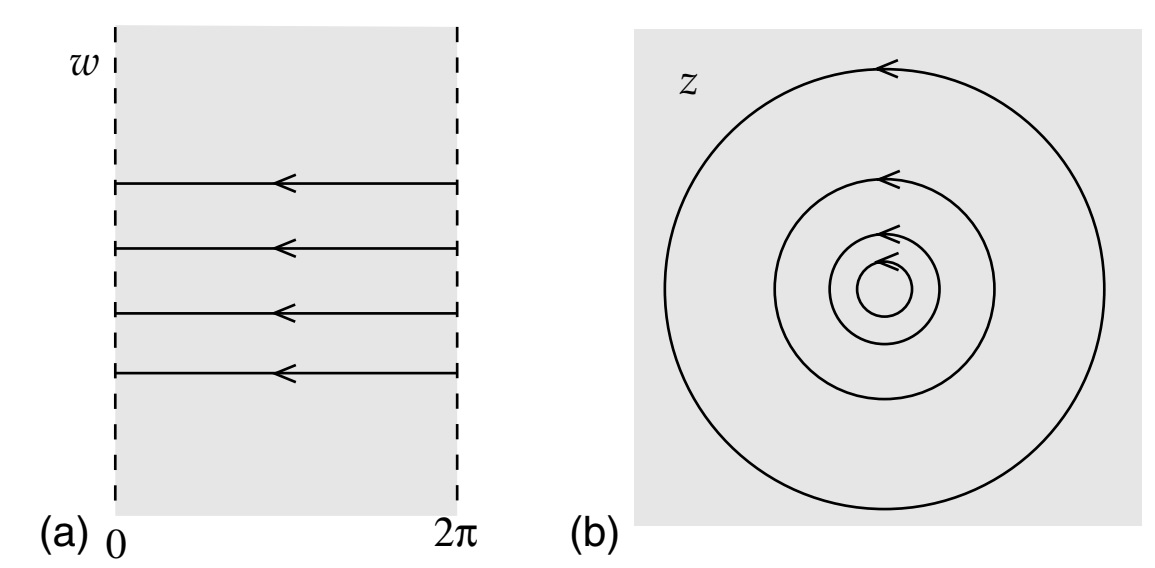
\includegraphics[width=0.8\textwidth,natwidth=866,natheight=426]{Fig2.3.jpg}\\
	\caption{Closed String Coordinates}
\end{center}
\end{figure}

在w坐标中,时间对应于$\sigma^{2}=\operatorname{Im} w$ 的移动. 在z坐标中,时间径向移动,原点是遥远的过去. 这些坐标通过一个共形变换相关. 对于理论的正则解释,w坐标是自然的,但z坐标也相当有用,并且大多数表达式都写在这个参考系中.\\
对于全纯或反全纯算符,我们可以做Laurent展开
\begin{equation}
T_{z z}(z)=\sum_{m=-\infty}^{\infty} \frac{L_{m}}{z^{m+2}}, \quad \tilde{T}_{\bar{z} \bar{z}}(\bar{z})=\sum_{m=-\infty}^{\infty} \frac{\tilde{L}_{m}}{\bar{z}^{m+2}}
\end{equation}
展开系数称为Virasoro生成元. 由围道积分给出
\begin{equation}\label{2.6.6}
L_{m}=\oint_{C} \frac{d z}{2 \pi i z} z^{m+2} T_{z z}(z)
\end{equation}
其中C以逆时针围绕原点的任意围道. 在$\sigma^2=0$时,Laurent展开就是一个普通的Fourier变换
\begin{subequations}
\begin{equation}
T_{w w}(w)=-\sum_{m=-\infty}^{\infty} \exp \left(i m \sigma^{1}-m \sigma^{2}\right) T_{m}
\end{equation}
\begin{equation}
T_{\bar{w} \bar{w}}(\bar{w})=-\sum_{m=-\infty}^{\infty} \exp \left(-i m \sigma^{1}-m \sigma^{2}\right) \tilde{T}_{m}
\end{equation}
\end{subequations}
其中
\begin{equation}\label{2.6.8}
T_{m}=L_{m}-\delta_{m, 0} \frac{c}{24}, \quad \tilde{T}_{m}=\tilde{L}_{m}-\delta_{m, 0} \frac{\tilde{c}}{24}
\end{equation}
$T_0$的额外偏移源于非张量变换(\ref{2.4.26})
\begin{equation}
T_{w w}=\left(\partial_{w} z\right)^{2} T_{z z}+\frac{c}{24}
\end{equation}
在$w=\sigma^{1}+i \sigma^{2}$系中,时间平移的Hamiltonian 是
\begin{equation}\label{2.6.10}
H=\int_{0}^{2 \pi} \frac{d \sigma^{1}}{2 \pi} T_{22}=L_{0}+\tilde{L}_{0}-\frac{c+\tilde{c}}{24}
\end{equation}
注意Laurent展开中的+2. 在Fourier变换中由于T的共形变换被抵消了. 类似地,一个权重h的全纯场的Laurent展开将在指数上包含h. \\
将时间$\operatorname{Im} w=\ln |z|$为常数的圆上的路径积分剪开. Virasoro生成元变成通常意义上的算符. 由于全纯性,积分(\ref*{2.6.6})独立于C,因而特别地,在时间平移下不变. 即它们是守恒荷,与共形不变相联系的荷. \\
一个重要的事实:流的OPE决定了对应荷的代数. 考察一般荷$Q_{i}, i=1,2$,给定为全纯流的围道积分
\begin{equation}
Q_{i}\{C\}=\oint_{C} \frac{d z}{2 \pi i} j_{i}
\end{equation}
考察组合
\begin{equation}\label{2.6.12}
Q_{1}\left\{C_{1}\right\} Q_{2}\left\{C_{2}\right\}-Q_{1}\left\{C_{3}\right\} Q_{2}\left\{C_{2}\right\}
\end{equation}
围道如图(\ref{Fig2.4}a)所示.\\
\begin{figure}
	\begin{center}
		%	\includegraphics[width=0.8\textwidth,bb=0 0 1299 596]{Fig2.3ClosedStringCoordinates.jpg}\\
		%1px=0.75pt
		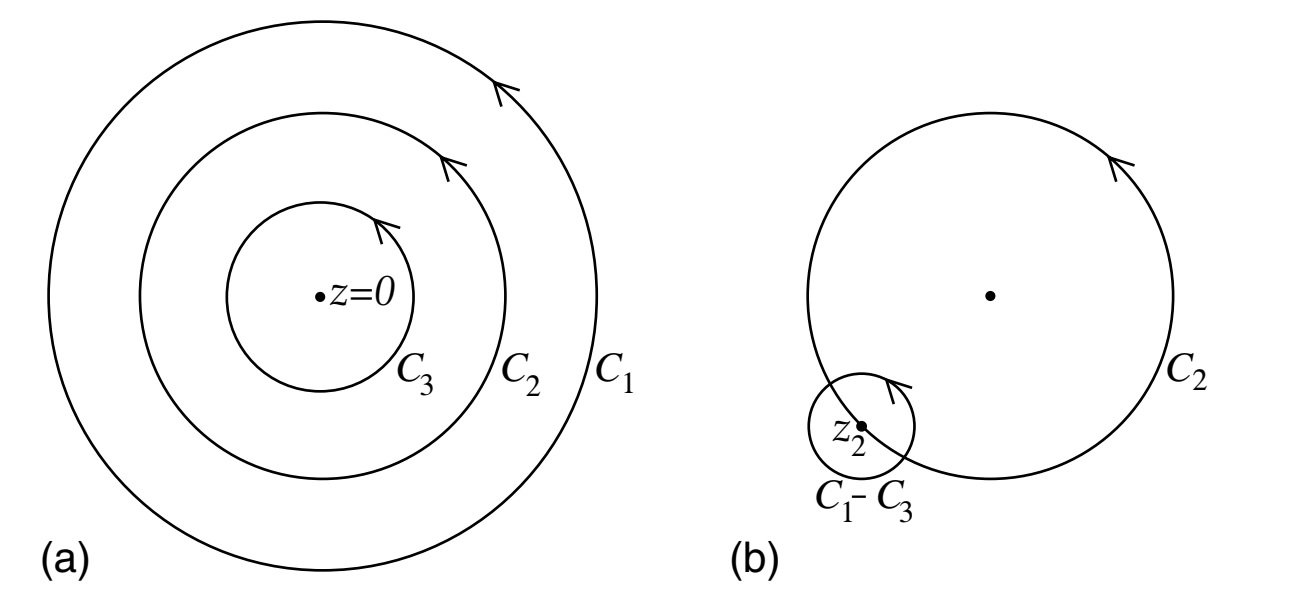
\includegraphics[width=0.8\textwidth,natwidth=974,natheight=447]{Fig2.4.jpg}\\
		\caption{Contours}\label{Fig2.4}
	\end{center}
\end{figure}

因子写成的序列是无关的,因为它们仅是一个路径积分中的积分变量(除非两个荷是反对易的. 在这种情况下会有一个额外的符号并且所有的对易子都会变成反对易子).\\
正如附录中所讨论的,当我们劈开路径积分以做一个算符解释. 决定算符序列的是时间顺序,在这里是
$t_{1}>t_{2}>t_{3}$. 对组合(\ref{2.6.12})的路径积分对应矩阵元
\begin{equation}
\hat{Q}_{1} \hat{Q}_{2}-\hat{Q}_{2} \hat{Q}_{1} \equiv\left[\hat{Q}_{1}, \hat{Q}_{2}\right]
\end{equation}
现在,对于围道$C_2$上的一给定点$z_2$,我们可以将$C_1, C_3$围道的差异进行变形,如图(\ref{Fig2.4}b)所示.\\
对易子因而由OPE的留数给出
\begin{equation}
\left[Q_{1}, Q_{2}\right]\left\{C_{2}\right\}=\oint_{C_{2}} \frac{d z_{2}}{2 \pi i} \operatorname{Res}_{z_{1} \rightarrow z_{2}} j_{1}\left(z_{1}\right) j_{2}\left(z_{2}\right)
\end{equation}
围道讨论允许我们在OPE与对易关系之间来回传递. 我们来强调一下,对于守恒流,知道了OPE中的奇异性等效于知道了对应荷的对易子代数. 将守恒荷$Q_{2}\left\{C_{2}\right\}$ 替换成任意算符,上面的讨论同样适用:
\begin{equation}
\left[Q, \mathscr{A}\left(z_{2}, \bar{z}_{2}\right)\right]=\operatorname{Res}_{z_{1} \rightarrow z_{2}} j\left(z_{1}\right) \mathscr{A}\left(z_{2}, \bar{z}_{2}\right)=\frac{1}{i \epsilon} \delta \mathscr{A}\left(z_{2}, \bar{z}_{2}\right)
\end{equation}
这正是熟悉的陈述:荷Q生成了相对应的变换. 类似地,对于反全纯流的围道积分
\begin{equation}
\tilde{Q}\{C\}=-\oint_{C} \frac{d \bar{z}}{2 \pi i} \tilde{\jmath}
\end{equation}
Ward等式与围道讨论暗示了
\begin{equation}
\left[\tilde{Q}, \mathscr{A}\left(z_{2}, \bar{z}_{2}\right)\right]=\overline{\operatorname{Res}}_{\bar{z}_{1} \rightarrow \bar{z}_{2}} \tilde{\jmath}\left(\bar{z}_{1}\right) \mathscr{A}\left(z_{2}, \bar{z}_{2}\right)=\frac{1}{i \epsilon} \delta \mathscr{A}\left(z_{2}, \bar{z}_{2}\right)
\end{equation}
将其应用于Virasoro代数(\ref{2.6.6}), 
\begin{equation}
\begin{array}{l}
\operatorname{Res}_{z_{1} \rightarrow z_{2}} z_{1}^{m+1} T\left(z_{1}\right) z_{2}^{n+1} T\left(z_{2}\right) \\
\quad=\operatorname{Res}_{z_{1} \rightarrow z_{2}} z_{1}^{m+1} z_{2}^{n+1}\left(\frac{c}{2 z_{12}^{4}}+\frac{2}{z_{12}^{2}} T\left(z_{2}\right)+\frac{1}{z_{12}} \partial T\left(z_{2}\right)\right)\\
=\frac{c}{12}\left(\partial^{3} z_{2}^{m+1}\right) z_{2}^{n+1}+2\left(\partial z_{2}^{m+1}\right) z_{2}^{n+1} T\left(z_{2}\right)+z_{2}^{m+n+2} \partial T\left(z_{2}\right) \\
=\frac{c}{12}\left(m^{3}-m\right) z_{2}^{m+n-1}+(m-n) z_{2}^{m+n+1} T\left(z_{2}\right)+\text { total derivative }
\end{array}
\end{equation}
其中$j_{m}(z)=z^{m+1} T(z)$.
那么右边的$z_2$围道积分给出Virasoro代数:
\begin{equation}\label{2.6.19}
\left[L_{m}, L_{n}\right]=(m-n) L_{m+n}+\frac{c}{12}\left(m^{3}-m\right) \delta_{m,-n}
\end{equation}
$\tilde{L}_{m}$满足中心荷为$\tilde{c}$ 的相同代数.
因而任何CFT有无限个守恒荷,即Virasoro生成元. 其作用在Hilbert空间中并满足代数(\ref{2.6.19}). 先关注几个简单的性质. 一般地,处理$L_{0}$ 和 $\tilde{L}_{0}$ 的本征态,生成元$L_{0}$ 满足
\begin{equation}
\left[L_{0}, L_{n}\right]=-n L_{n}
\end{equation}
如果$|\psi\rangle$ 是 $L_{0}$的本征值为h的本征态,那么
\begin{equation}
L_{0} L_{n}|\psi\rangle=L_{n}\left(L_{0}-n\right)|\psi\rangle=(h-n) L_{n}|\psi\rangle
\end{equation}
所以$L_n|\psi\rangle$ 是本征值为h-n的本征态,n<0的生成元提高$L_{0}$的本征值,而n>0则降低它.\\
三个生成元$L_{0}$ , $L_{\pm 1}$构成没有中心荷的闭代数:
\begin{equation}
\left[L_{0}, L_{1}\right]=-L_{1}, \quad\left[L_{0}, L_{-1}\right]=L_{-1}, \quad\left[L_{1}, L_{-1}\right]=2 L_{0}
\end{equation}
这是代数$SL(2,R)$,与SU(2)相差一个符号. 对于权重$(h,0)$的全纯张量场$\mathcal{O}$的Laurent系数
\begin{equation}
\mathcal{O}(z)=\sum_{m=-\infty}^{\infty} \frac{\mathcal{O}_{m}}{z^{m+h}}
\end{equation}
从OPE(\ref{2.4.16})得到对易子
\begin{equation}
\left[L_{m}, \mathcal{O}_{n}\right]=[(h-1) m-n] \mathcal{O}_{m+n}
\end{equation}
又一次, n>0的模减小$L_0$,n<0的模增大$L_0$.\\
\begin{proof}
令
$j_{m}(z)=z^{m+1} T(z), \quad j_{n}(z)=z^{n+h-1} \mathcal{O}(z)$
$$
\begin{array}{l}
\operatorname{Res}_{z_1 \rightarrow z_2}  z_1^{m+1} T\left(z_{1}\right) z_2^{n+h-1} \mathcal{O}(z_{2})\\
=\operatorname{Res}_{z_1 \rightarrow z_2} z_1^{m+1} z_2^{n+h-1}\left(\frac{h}{z_{12}^2} O(z_2)+\frac{1}{z_{12}} \partial \mathcal{O}(z_2)\right)\\
=h(\partial z_2^{m+1})z_2^{n+h-1}\mathcal{O}(z_2)+z_2^{m+n+h}\partial\mathcal{O}(z_2)\\
=h(m+1)z_2^{m+n+h-1}\mathcal{O}(z_2)-(m+n+h)z_2^{m+n+h-1}\mathcal{O}(z_2)+div
\end{array}
$$
所以第一项
$$h(m+1)z_2^{m+n+h-1}\mathcal{O}(z_2) \sim h(m+1) \sum \mathcal{O}_q z_2^{m+n-q-1} \sim h(m+1)\mathcal{O}_{m+n}$$
第二项
$$
\begin{array}{l}
=-(m+n+h) z_{2}^{m+n+h-1} \sum \frac{\mathcal{O}_{q}}{z_{2}^{q+h}} \\
\sim -(m+n+h) \sum \mathcal{O}_{q} z_{2}^{m+n-q-1} \\
\sim-(m+n+h) \mathcal{O}_{m+n}
\end{array}
$$

二者相加得
$$\left[L_{m}, \mathcal{O}_{n}\right]=[(h-1) m-n] \mathcal{O}_{m+n}$$
\end{proof}

在开弦中,令
\begin{equation}
0 \leq \operatorname{Re} w \leq \pi \quad \Leftrightarrow \quad \operatorname{Im} z \geq 0
\end{equation}
其中
$z=-\exp (-i w)$. 
坐标区域如图(\ref{Fig2.5}).
\begin{figure}
	\begin{center}
		%	\includegraphics[width=0.8\textwidth,bb=0 0 778 341]{Fig2.3ClosedStringCoordinates.jpg}\\
		%1px=0.75pt
		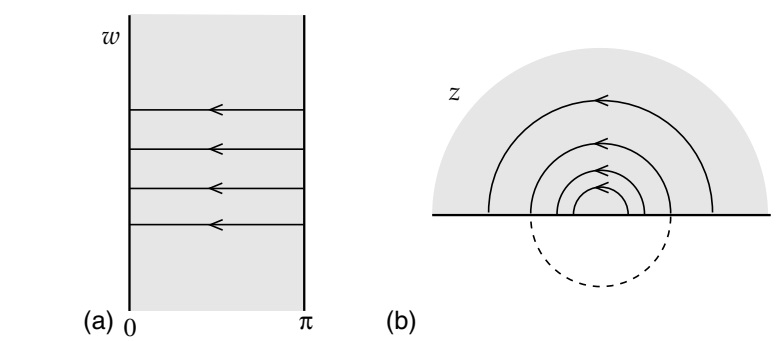
\includegraphics[width=0.8\textwidth,natwidth=584,natheight=256]{Fig2.5.jpg}\\
		\caption{Contours}\label{Fig2.5}
	\end{center}
\end{figure}
作为边界,能动量满足
\begin{equation}\label{2.6.26}
T_{a b} n^{a} t^{b}=0
\end{equation}
其中$n^{a}$ , $t^{b}$是法向和切向矢量. 为了看到这点,考察边界是直线的坐标系. 边界的出现破坏了法向的平移不变性,但不破坏切向,使得流$T_{a b} t^{b}$ 依旧是守恒的. 那么边界条件(\ref{2.6.26})就是陈述流出边界的流是零. 在目前的情况下,这变成
\begin{equation}
T_{w w}=T_{\bar{w} \bar{w}}, \operatorname{Re} w=0, \pi \quad \Leftrightarrow \quad T_{z z}=T_{\bar{z} \bar{z}}, \operatorname{Im} z=0
\end{equation}
使用doubling trick是方便的. 将下半z平面中的$T_{zz}$定义为$T_{\bar{z} \bar{z}}$在上半平面的镜像点$z^{\prime}=\bar{z}$处的值:
\begin{equation}
T_{z z}(z) \equiv T_{\bar{z} \bar{z}}\left(\bar{z}^{\prime}\right), \quad \operatorname{Im} z<0
\end{equation}
运动方程与边界条件总结为:$T_{z z}$在整个复平面全纯.
仅存在一组Virasoro代数,因为边界条件耦合了$T$ 和 $\widetilde{T}$:
\begin{equation}
\begin{aligned}
L_{m} &=\frac{1}{2 \pi i} \int_{C}\left(d z z^{m+1} T_{z z}-d \bar{z} \bar{z}^{m+1} T_{\bar{z} \bar{z}}\right) \\
&=\frac{1}{2 \pi i} \oint d z z^{m+1} T_{z z}(z)
\end{aligned}
\end{equation}
第一行中,围道是中心为原点的半圆;第二行,我们使用了doubling trick将$L_m$写成了闭合围道. 又一次,这些情况满足Virasoro代数
\begin{equation}
\left[L_{m}, L_{n}\right]=(m-n) L_{m+n}+\frac{c}{12}\left(m^{3}-m\right) \delta_{m,-n}
\end{equation}

\section{模式展开}%{2.7 Mode expansions}

\centerline{\Large 自由标量}
在自由场论中,场分解成谐振子,并且频谱与能动量张量可以以模的形式上
给出. 我们从闭弦开始. 在$X^\mu$的理论中, $\partial X$ 和 $\bar{\partial} X$是反全纯的. 所以有类似T的Laurent展开:
\begin{equation}\label{2.7.1}
\partial X^{\mu}(z)=-i\left(\frac{\alpha^{\prime}}{2}\right)^{1 / 2} \sum_{m=-\infty}^{\infty} \frac{\alpha_{m}^{\mu}}{z^{m+1}}, \quad \bar{\partial} X^{\mu}(\bar{z})=-i\left(\frac{\alpha^{\prime}}{2}\right)^{1 / 2} \sum_{m=-\infty}^{\infty} \frac{\tilde{\alpha}_{m}^{\mu}}{\bar{z}^{m+1}}
\end{equation}
等效地,
\begin{subequations}\label{2.7.2}
\begin{equation}
\alpha_{m}^{\mu}=\left(\frac{2}{\alpha^{\prime}}\right)^{1 / 2} \oint \frac{d z}{2 \pi} z^{m} \partial X^{\mu}(z)
\end{equation}
\begin{equation}
\tilde{\alpha}_{m}^{\mu}=-\left(\frac{2}{\alpha^{\prime}}\right)^{1 / 2} \oint \frac{d \bar{z}}{2 \pi} \bar{z}^{m} \bar{\partial} X^{\mu}(\bar{z})
\end{equation}
\end{subequations}
 $X^\mu$的单值性暗示着$\alpha_{0}^{\mu}=\tilde{\alpha}_{0}^{\mu}$ ,更进一步,时空平移的Noether流是$i \partial_{a} X^{\mu} / \alpha^{\prime}$ ,所以时空动量
\begin{equation}\label{2.7.3}
p^{\mu}=\frac{1}{2 \pi i} \oint_{C}\left(d z j^{\mu}-d \bar{z} \tilde{\jmath}^{\mu}\right)=\left(\frac{2}{\alpha^{\prime}}\right)^{1 / 2} \alpha_{0}^{\mu}=\left(\frac{2}{\alpha^{\prime}}\right)^{1 / 2} \tilde{\alpha}_{0}^{\mu}
\end{equation}
对表达式(\ref{2.7.1}) 积分给出
\begin{equation}
X^{\mu}(z, \bar{z})=x^{\mu}-i \frac{\alpha^{\prime}}{2} p^{\mu} \ln |z|^{2}+i\left(\frac{\alpha^{\prime}}{2}\right)^{1 / 2} \sum_{m=-\infty , m \neq 0}^{\infty} \frac{1}{m}\left(\frac{\alpha_{m}^{\mu}}{z^{m}}+\frac{\tilde{\alpha}_{m}^{\mu}}{\bar{z}^{m}}\right)
\end{equation}
无论是从标准正则对易出发,还是从围道讨论或者XXOPE,可以给出
\begin{subequations}
\begin{equation}
\left[\alpha_{m}^{\mu}, \alpha_{n}^{v}\right]=\left[\tilde{\alpha}_{m}^{\mu}, \tilde{\alpha}_{n}^{v}\right]=m \delta_{m,-n} \eta^{\mu v}
\end{equation}
\begin{equation}
\left[x^{\mu}, p^{v}\right]=i \eta^{\mu v}
\end{equation}
\end{subequations}
其他对易子为零. 这个谱通过从态$|0 ; k\rangle$ 开始而给出. 这个态动量为$k^\mu$ 且被所有下降模n>0 的$\alpha_n^\mu$ 所湮灭 而对上升模(n<0) ,则以所有可能的方式作用.\\
我们现在希望以模算符的形式展开Virasoro生成元. 将$X^\mu$ 的Laurent展开式插入到能动量张量(\ref{2.4.4}) 并集合z的给定阶的项,给出
\begin{equation}\label{2.7.6}
L_{m} \sim \frac{1}{2} \sum_{n=-\infty}^{\infty} \alpha_{m-n}^{\mu} \alpha_{\mu n}
\end{equation}
 ~代表我们忽略了算符的顺序. 对于$m\neq 0$ , 展开式(\ref{2.7.6}) 是定义良好的且正确的————每一项的模算符对易所以序列不重要. 对于m=0, 将下降算符放在右边并引入一规范序列常数
 \begin{equation}
 L_{0}=\frac{\alpha^{\prime} p^{2}}{4}+\sum_{n=1}^{\infty}\left(\alpha_{-n}^{\mu} \alpha_{\mu n}\right)+a^{X}
 \end{equation}
 我们在1.3节中遇到同一问题,在那里我们以一种启发式的方法处理 现在左边以::一序列能动量张量的Laurent系数的形式有了一个有限且明确的定义,所以规范序列常数是有限且可计算的. 有几种方式可以决定它,最简单的是用Virasoro代数:
 \begin{equation}\label{2.7.8}
 2 L_{0}|0 ; 0\rangle=\left(L_{1} L_{-1}-L_{-1} L_{1}\right)|0 ; 0\rangle=0
 \end{equation}
 因而
 \begin{equation}
 a^{X}=0
 \end{equation}
 这里我们使用了$L_1, L_{-1}$ 的已知形式:每一项要么包含下降算符,要么包含$p^\mu$. 因而湮灭$|0 ; 0\rangle$. \\
从OPE中,我们决定了Virasoro代数的中心荷. 它也可以从Virasoro代数的模算符表达式直接得出.\\
引入一个新的记法. 符号${}_\circ^\circ {}_\circ^\circ$ 代表产生-湮灭正规序列,将所有下降算符放在所有产生算符右边. 注意交换反对易算符时有一个负号. 由于这个原因,我们将$p^\mu$纳入下降算符,将$x^\mu$纳入上升算符. 在这个记号下,我么可以写
\begin{equation}\label{2.7.10}
L_{m}=\frac{1}{2} \sum_{n=-\infty}^{\infty}{}_{\circ}^{\circ} \alpha_{m-n}^{\mu} \alpha_{\mu n}{}_{\circ}^{\circ}
\end{equation}
我们现在引入了两种正规序列形式,即共形正规序列::与产生-湮灭正规序列${}_\circ^\circ {}_\circ^\circ$ . 前者是有用的,因为它所产生的算符,其OPE与共形变换性质是简单的;后者可能对于读者更为熟悉,在处理算符的矩阵元时是有用的. 我们现在要给出二者关系. 从比较编时乘积与产生-湮灭正规乘积开始. 对于 $|z|>\left|z^{\prime}\right|$的乘积$X^{\mu}(z, \bar{z}) X^{\nu}\left(z^{\prime}, \bar{z}^{\prime}\right)$ ,代入模展开,并将$X^{\mu}(z, \bar{z})$ 中的下降算符挪到右边,保留对易子的痕迹给出
\begin{equation}\label{2.7.11}
\begin{aligned}
X^{\mu}(z, \bar{z}) X^{\nu}\left(z^{\prime}, \bar{z}^{\prime}\right)=&{ }_{\circ}^{\circ} X^{\mu}(z, \bar{z}) X^{\nu}\left(z^{\prime}, \bar{z}^{\prime}\right)  { }_{\circ}^{\circ} \\
&+\frac{\alpha^{\prime}}{2} \eta^{\mu \nu}\left[-\ln |z|^{2}+\sum_{m=1}^{\infty} \frac{1}{m}\left(\frac{z^{\prime m}}{z^{m}}+\frac{\bar{z}^{\prime m}}{\bar{z}^{m}}\right)\right]\\
=&{ }_{\circ}^{\circ} X^{\mu}(z, \bar{z}) X^{\nu}\left(z^{\prime}, \bar{z}^{\prime}\right)  { }_{\circ}^{\circ}-\frac{\alpha^{\prime}}{2} \eta^{\mu \nu}\ln |z-z^\prime|^{2}
\end{aligned}
\end{equation}
由于$|z|>\left|z^{\prime}\right|$,这里左边是编时的而且求和收敛. 定义(2.1.21)给出的编时乘积与共形正规乘积的关系(以路径积分语言,所以右边的乘积在算符体系下是编时的). 这与(\ref{2.7.11})是相同的,使得
\begin{equation}\label{2.7.12}
{ }_\circ^{\circ} X^{\mu}(z, \bar{z}) X^{\nu}\left(z^{\prime}, \bar{z}^{\prime}\right){}_\circ^{\circ}=: X^{\mu}(z, \bar{z}) X^{\nu}\left(z^{\prime}, \bar{z}^{\prime}\right):
\end{equation}
这种关系在普遍的CFT中并不成立,并且实际上,$p^\mu$与下降算符的某些组合给出更简单的结果. 对于算符的w形式的共形正规序列这也不成立.
从(\ref{2.7.12})可以立即写出模展开(\ref{2.7.10}) 给出$a^x=0$的二阶导数.\\
超过两个$X^\mu$的产生-湮灭正规乘积与::序列有相同的组合学因子. 即,它们从编时乘积中,通过对所有的收缩获得(场论中的Wick定理). 为了将算符的正规序列从一种形式转化到另一种形式,利用两点函数的差对所有收缩求和. 即,如果我们有两类序列
\begin{equation}
\left[X^{\mu}(z, \bar{z}) X^{v}\left(z^{\prime}, \bar{z}^{\prime}\right)\right]_{1}=\left[X^{\mu}(z, \bar{z}) X^{v}\left(z^{\prime}, \bar{z}^{\prime}\right)\right]_{2}+\eta^{\mu v} \Delta\left(z, \bar{z}, z^{\prime}, \bar{z}^{\prime}\right)
\end{equation}
那么对于一般算符$\mathscr{F}$
\begin{equation}
[\mathscr{F}]_{1}=\exp \left(\frac{1}{2} \int d^{2} z d^{2} z^{\prime} \Delta\left(z, \bar{z}, z^{\prime}, \bar{z}^{\prime}\right) \frac{\delta}{\delta X^{\mu}(z, \bar{z})} \frac{\delta}{\delta X_{\mu}\left(z^{\prime}, \bar{z}^{\prime}\right)}\right)[\mathscr{F}]_{2}
\end{equation}
对于线性伸缩子CFT,Laurent展开与对易子不变,而Virasoro生成元包含一个额外项
\begin{equation}
L_{m}=\frac{1}{2} \sum_{n=-\infty}^{\infty}{}_{\circ}^{\circ} \alpha_{m-n}^{\mu} \alpha_{\mu n}{}_{\circ}^{\circ}+i\left(\frac{\alpha^{\prime}}{2}\right)^{1 / 2}(m+1) V^{\mu} \alpha_{\mu m}
\end{equation}

\centerline{\Large bc CFT}
场b和c有Laurent展开
\begin{equation}
b(z)=\sum_{m=-\infty}^{\infty} \frac{b_{m}}{z^{m+\lambda}}, \quad c(z)=\sum_{m=-\infty}^{\infty} \frac{c_{m}}{z^{m+1-\lambda}}
\end{equation}
精确些,如果$\lambda$是整数,它们仅是Laurent展开. 半整数的情况也是有趣的,我们将在第10章细致地处理它. OPE给出反对易子
\begin{equation}
\left\{b_{m}, c_{n}\right\}=\delta_{m,-n}
\end{equation}
首先考察被所有n>0的算符消灭的态. $b_0, c_0$振子代数生成两个这样的基态$|\downarrow\rangle$ 和 $|\uparrow\rangle$. 其有性质
\begin{subequations}
\begin{equation}
b_{0}|\downarrow\rangle=0, \quad b_{0}|\uparrow\rangle=|\downarrow\rangle,
\end{equation}
\begin{equation}
c_{0}|\downarrow\rangle=|\uparrow\rangle, \quad c_{0}|\uparrow\rangle=0,
\end{equation}
\begin{equation}
b_{n}|\downarrow\rangle=b_{n}|\uparrow\rangle=c_{n}|\downarrow\rangle=c_{n}|\uparrow\rangle=0, \quad n>0
\end{equation}
\end{subequations}
普通的态通过用n<0的模作用其上获得,不过由于反对易,最多作用一次. 由于之后的某些原因,将$b_0$与下降算符组队,$c_0$与上升算符组队将是方便的,所以我们挑出$|\downarrow\rangle$ 作为幽灵真空$|0\rangle$.在弦论中我们将有一个全纯bc理论,与反全纯$\tilde{b} \tilde{c}$ 理论. 每一个有$\lambda=2$,因而闭弦频谱包含之上的两个的乘积.\\
Virasoro生成元是
\begin{equation}
L_{m}=\sum_{n=-\infty}^{\infty}(m \lambda-n) {}_\circ^\circ b_{n} c_{m-n}{}_\circ^\circ+\delta_{m, 0} a^{\mathrm{g}}
\end{equation}
序列常数. 可以(\ref{2.7.8})那样决定,其给出
\begin{equation}
\begin{aligned}
2 L_{0}|\downarrow\rangle &=\left(L_{1} L_{-1}-L_{-1} L_{1}\right)|\downarrow\rangle \\
&=\left(\lambda b_{0} c_{1}\right)\left[(1-\lambda) b_{-1} c_{0}\right]|\downarrow\rangle=\lambda(1-\lambda)|\downarrow\rangle
\end{aligned}
\end{equation}
因而$a^{\mathrm{g}}=\frac{1}{2} \lambda(1-\lambda)$
并且
\begin{equation}
L_{m}=\sum_{n=-\infty}^{\infty}(m \lambda-n) {}_\circ^\circ b_{n} c_{m-n}{}_\circ^\circ+\frac{\lambda(1-\lambda)}{2} \delta_{m, 0}
\end{equation}
常数也可以通过解出::和${}_\circ^\circ {}_\circ^\circ$的关系获得. 对于幽灵数流(\ref{2.5.14}),  荷是
\begin{equation}\label{2.7.22}
\begin{aligned}
N^{\mathrm{g}} &=-\frac{1}{2 \pi i} \int_{0}^{2 \pi} d w j_{w} \\
&=\sum_{n=1}^{\infty}\left(c_{-n} b_{n}-b_{-n} c_{n}\right)+c_{0} b_{0}-\frac{1}{2}
\end{aligned}
\end{equation}
它满足
\begin{equation}
\left[N^{\mathrm{g}}, b_{m}\right]=-b_{m}, \quad\left[N^{\mathrm{g}}, c_{m}\right]=c_{m}
\end{equation}
因而c数减去b数是激发. 基态有鬼数$\pm \frac{1}{2}$
\begin{equation}
N^{\mathrm{g}}|\downarrow\rangle=-\frac{1}{2}|\downarrow\rangle, \quad N^{\mathrm{g}}|\uparrow\rangle=\frac{1}{2}|\uparrow\rangle
\end{equation}
这依赖于序列常数的值,可以进行猜测. 理由是基态平均幽灵数应该是零:鬼数在$b \leftrightarrow c$ 下改变符号.\\

\centerline{\Large 开弦}
在开弦中,Neumann边界条件变成了实轴上的$\partial_z X^{\mu}=\partial_{\bar{z}} X^{\mu}$.
仅存在一组模,边界条件要求展开式(\ref{2.7.1})中$\alpha_{m}^{\mu}=\tilde{\alpha}_{m}^{\mu}$. 时空动量积分 (\ref{2.7.3})只积半圆. 所以现在的归一化是
\begin{equation}
\alpha_{0}^{\mu}=\left(2 \alpha^{\prime}\right)^{1 / 2} p^{\mu}
\end{equation}
那么$X^\mu$的展开是
\begin{equation}
X^{\mu}(z, \bar{z})=x^{\mu}-i \alpha^{\prime} p^{\mu} \ln |z|^{2}+i\left(\frac{\alpha^{\prime}}{2}\right)^{1 / 2} \sum_{m=-\infty , m \neq 0}^{\infty} \frac{\alpha_{m}^{\mu}}{m}\left(z^{-m}+\bar{z}^{-m}\right)
\end{equation}
另外
\begin{equation}
L_{0}=\alpha^{\prime} p^{2}+\sum_{n=1}^{\infty} \alpha_{-n}^{\mu} \alpha_{\mu n}
\end{equation}
对易子像往常一样
\begin{equation}
\left[\alpha_{m}^{\mu}, \alpha_{n}^{\nu}\right]=m \delta_{m,-n} \eta^{\mu \nu}, \quad\left[x^{\mu}, p^{\nu}\right]=i \eta^{\mu \nu}
\end{equation}
对于bc理论,与弦相关的边界条件是
\begin{equation}
c(z)=\tilde{c}(\bar{z}), \quad b(z)=\tilde{b}(\bar{z}), \quad \operatorname{Im} z=0
\end{equation}
这是z坐标形式,其中边界在实轴上. 那么我们可以用双倍叠加将上半平面的全纯场和反全纯场写成整个平面中的全纯场的形式
\begin{equation}
c(z) \equiv \tilde{c}\left(\bar{z}^{\prime}\right), \quad b(z) \equiv \tilde{b}\left(\bar{z}^{\prime}\right), \quad \operatorname{Im}(z) \leq 0, z^{\prime}=\bar{z}
\end{equation}
因而对于单个b和c,开弦有单组Laurent展开.

\section{顶角算子}%{2.8 Vertex operators}

在量子场论中,一方面,既有理论的态空间;另一方面,又有定域算符的集合. 在共形场论中,它们之间有一个简单且有用的同构,CFT在一个圆上量子化. 考察w坐标中半无限大的圆柱
\begin{equation}
0 \leq \operatorname{Re} w \leq 2 \pi, \quad w \sim w+2 \pi, \quad \operatorname{Im} w \leq 0
\end{equation}
其映射到$z=\exp (-i w)$ 下的一个单位圆盘.  如图(\ref{Fig2.6})所示.
\begin{figure}
\begin{center}
		%	\includegraphics[width=0.8\textwidth,bb=0 0 714 503]{Fig2.3ClosedStringCoordinates.jpg}\\
		%1px=0.75pt
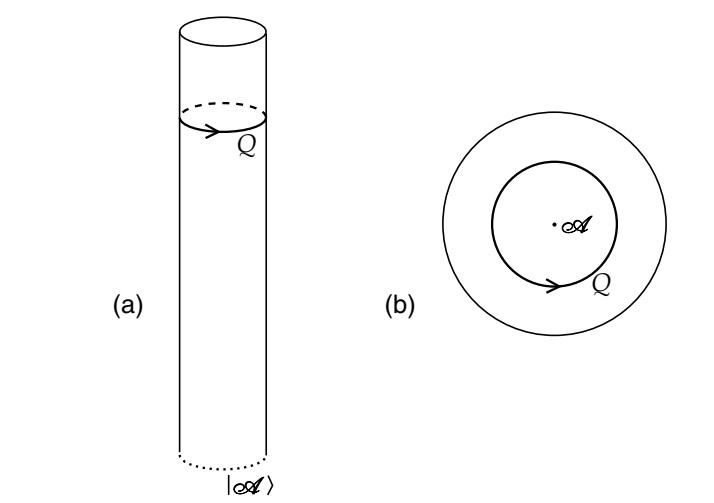
\includegraphics[width=0.8\textwidth,natwidth=535,natheight=377]{Fig2.6.jpg}\\
\caption{(a) A semi-infinite cylinder in w, with initial state $|\mathscr{A}\rangle$ and charge Q. 
(b)The conformally equivalent unit disk with local operator $\mathscr{A}$ and contour integral for Q}\label{Fig2.6}
\end{center}
\end{figure}
对于自由场论,容易得到这个同构的详细形式. 假定有一守恒荷Q以图(\ref{Fig2.6}a)那样的方式作用在态$|\mathscr{A}\rangle$ 上. 通过使用OPE计算图(\ref{Fig2.6}b)中的围道积分,可以发现对应的定域算符. 对应于单位算符,我们等同态$|1\rangle$. 在原点没有算符时,$\partial X^{\mu}$ 和 $\bar{\partial} X^{\mu}$在图(\ref{Fig2.6}b)Q的围道内是全纯和反全纯的. 那么,定义$m \geq 0$ 的$\alpha_{m}^{\mu}$ and $\tilde{\alpha}_{m}^{\mu}$的围道积分(\ref{2.7.2})没有极点因而为零. 因而$|1\rangle$ 被这些模消灭,这表明它是基态
\begin{equation}
|1\rangle=|0 ; 0\rangle
\end{equation}
现在考察,例如m为正的态$\alpha_{-m}^{\mu}|1\rangle$. 过渡到图(\ref{Fig2.6}b),$Q=\alpha_{-m}^{\mu}$,场在围道内是全纯的
\begin{equation}\label{2.8.3}
\alpha_{-m}^{\mu}=\left(\frac{2}{\alpha^{\prime}}\right)^{1 / 2} \oint \frac{d z}{2 \pi} z^{-m} \partial X^{\mu}(z) \rightarrow\left(\frac{2}{\alpha^{\prime}}\right)^{1 / 2} \frac{i}{(m-1) !} \partial^{m} X^{\mu}(0)
\end{equation}
因而
\begin{equation}
\alpha_{-m}^{\mu}|1\rangle \cong\left(\frac{2}{\alpha^{\prime}}\right)^{1 / 2} \frac{i}{(m-1) !} \partial^{m} X^{\mu}(0), \quad m \geq 1
\end{equation}
类似地
\begin{equation}
\tilde{\alpha}_{-m}^{\mu}|1\rangle \cong\left(\frac{2}{\alpha^{\prime}}\right)^{1 / 2} \frac{i}{(m-1) !} \bar{\partial}^{m} X^{\mu}(0), \quad m \geq 1
\end{equation}
当$\alpha_{-m}^{\mu}$ or $\tilde{\alpha}_{-m}^{\mu}$ 作用在一般态$|\mathscr{A}\rangle$上时,这个对应依旧成立. 如果$: \mathscr{A}(0,0):$ 是任意的正规序列算符,在$\partial X^{\mu}(z)$ 与 $: \mathscr{A}(0,0)$ : 的算符乘积中可能会有奇异性. 但不难验证
\begin{equation}
\alpha_{-m}^{\mu}: \mathscr{A}(0,0):=: \alpha_{-m}^{\mu} \mathscr{A}(0,0):
\end{equation}
对于m>0成立. 这是因为该收缩的围道积分将不可能有单奇点,那么可以在正规序列中进行相同的运算(\ref{2.8.3}). 因而有数个$\alpha$振子激发的态作为相对应算符的::正规乘积出现
\begin{subequations}\label{2.8.7}
\begin{equation}
\alpha_{-m}^{\mu} \rightarrow i\left(\frac{2}{\alpha^{\prime}}\right)^{1 / 2} \frac{1}{(m-1) !} \partial^{m} X^{\mu}(0), \quad m \geq 1
\end{equation}
\begin{equation}
\tilde{\alpha}_{-m}^{\mu} \rightarrow i\left(\frac{2}{\alpha^{\prime}}\right)^{1 / 2} \frac{1}{(m-1) !} \bar{\partial}^{m} X^{\mu}(0), \quad m \geq 1
\end{equation}
\end{subequations}
类似地
\begin{equation}\label{2.8.8}
x_{0}^{\mu} \rightarrow X^{\mu}(0,0)
\end{equation}
通过用(\ref{2.8.7}) 和(\ref{2.8.8}) 左边的算符作用在$|1\rangle$ 上可以获得任何算符. 那么对应该态的算符由右边相对应的定域算符的::正规乘积给定. 例如
\begin{equation}
|0 ; k\rangle \cong: e^{i k \cdot X(0,0)}:
\end{equation}
这是很容易理解的:在平移$X^{\mu} \rightarrow X^{\mu}+a^{\mu}$ 下,态与相对应算符由同一平移, 被乘以$\me ^{\mi ka}$. \\
同一方法适用于bc理论. 明晰起见,我们指定$\lambda=2$的情况. 这是Boson弦论感兴趣的. 从Laurent展开与围道讨论给出
\begin{equation}\label{2.8.10}
b_{m}|1\rangle=0, \quad m \geq-1, \quad c_{m}|1\rangle=0, \quad m \geq 2
\end{equation}
注意Laurent展开指数中的飘移,它源于b和c的共形权重. 单位算符不再映射到基态上. 反而,关系(\ref{2.8.10})决定了
\begin{equation}
|1\rangle=b_{-1}|\downarrow\rangle
\end{equation}
上升算符的平移是直接的
\begin{subequations}
\begin{equation}
b_{-m} \rightarrow \frac{1}{(m-2) !} \partial^{m-2} b(0), \quad m \geq 2
\end{equation}
\begin{equation}
c_{-m} \rightarrow \frac{1}{(m+1) !} \partial^{m+1} c(0), \quad m \geq-1
\end{equation}
\end{subequations}
注意,鬼数为-3/2的态$b_{-1}|\downarrow\rangle$映射到鬼数为0的单位算符,而鬼数为-1/2的态$|\downarrow\rangle$映射到鬼数为1的算符c. 这一差异源于鬼数流的非张量性质(\ref{2.5.17})
\begin{equation}
\left(\partial_{z} w\right) j_{w}(w)=j_{z}(z)+q_{0} \frac{\partial_{z}^{2} w}{\partial_{z} w}=j_{z}(z)-\frac{q_{0}}{z}
\end{equation}
其中$q_{0}=\lambda-\frac{1}{2}=\frac{3}{2}$. 圆柱参考系表达式(\ref{2.7.22})通常定义了态的鬼数,而图(\ref{Fig2.6})的围道讨论将顶点算符的鬼数与极坐标系荷关系起来
\begin{equation}
Q^{\mathrm{g}} \equiv \frac{1}{2 \pi i} \oint d z j_{z}=N^{\mathrm{g}}+q_{0}
\end{equation}
这也适用于其他荷:对于张量流,态与相对应算符的荷是相等的.\\
上面大多数讨论可扩张到$\beta\gamma$理论,但在超弦下存在一定困难. \\
本节所有概念可扩展至开弦,半无限大带
\begin{equation}
0 \leq \operatorname{Re} w \leq \pi, \quad \operatorname{Im} w \leq 0
\end{equation}
映射至一个半圆盘;上半平面与单位圆的交叠映射为$z=-\exp (-i w)$;初态又一次映射至原点,其在边界上,所以存在同构
\begin{equation}
\text { local operators on the boundary边界上的局域算符 } \leftrightarrow \text { states on the interval 交界上的态}
\end{equation}
细节与之上相同. 双重技巧在围道讨论中是有用的.

\centerline{\Large 路径积分推导}
考察z平面的一个圆盘,其在原点处有定域算符$\mathscr{A}$,并在路径积分场中,在单位圆上取固定的边界值$\phi_{\mathrm{b}}$,对圆盘内部场$\phi_i$的路径积分且$\phi_{\mathrm{b}}$保持固定产生了泛函$\Psi_{\mathscr{A}}[\phi_{\mathrm{b}}]$
\begin{equation}
	\Psi_{\mathscr{A}}\left[\phi_{\mathrm{b}}\right]=\int\left[d \phi_{\mathrm{i}}\right]_{\phi_{\mathrm{b}}} \exp \left(-S\left[\phi_{\mathrm{i}}\right]\right) \mathscr{A}(0)
\end{equation}
场的泛函是态的Schrodinger表示,所以这是从算符到态的映射Schrodinger表示,其为每个场构形赋予了一个复振幅,有很多用途.\\
以另一种方式,从某个态$\Psi[\phi_{\mathrm{b}}]$开始. 考察在圆环区域$1 \geq|z| \geq r$ 上的路径积分,其中外圆上的$\phi_{\mathrm{b}}$ 固定,而沿着内圆对$\phi_{\mathrm{b}}^\prime$ 作如下积分:
\begin{equation}\label{2.8.18}
\int\left[d \phi_{\mathrm{b}}^{\prime}\right]\left[d \phi_{\mathrm{i}}\right]_{\phi_{\mathrm{b}}, \phi_{\mathrm{b}}^{\prime}} \exp \left(-S\left[\phi_{\mathrm{i}}\right]\right) r^{-L_{0}-\tilde{L}_{0}} \Psi\left[\phi_{\mathrm{b}}^{\prime}\right]
\end{equation}
即这个积分被赋予权重$r^{-L_{0}-\tilde{L}_{0}} \Psi\left[\phi_{\mathrm{b}}^{\prime}\right]$. 现在,对圆盘的路径积分恰好对应从 $|z|=r$到 $|z|=1$的传播,其等价于用算符 $r^{+L_{0}+\tilde{L}_{0}}$作用. 这抵消了作用在$\Phi$上的算符,所以(\ref{2.8.18})又一次是
$\Psi[\phi_{\mathrm{b}}]$. 现在取$r\to 0$的极限,圆环变成圆盘,而在内圆上的路径积分极限可以认为是在原点处定义了某个定域算符. 通过构建,圆盘上的路径积分与这个算符重新产生了边界上的$\Psi[\phi_{\mathrm{b}}]$. 我们来显示地处理单自由标量场X. 在单位圆上展开
\begin{equation}
X_{\mathrm{b}}(\theta)=\sum_{n=-\infty}^{\infty} X_{n} e^{i n \theta}, \quad X_{n}^{*}=X_{-n}
\end{equation}
边界态$\Psi[X_b]$可以认为是所有$X_n$的函数. 首先辨认出对应于单位算符的态. 由无插入的路径积分给定
\begin{equation}
\Psi_{1}\left[X_{\mathrm{b}}\right]=\int\left[d X_{\mathrm{i}}\right]_{X_{\mathrm{b}}} \exp \left(-\frac{1}{2 \pi \alpha^{\prime}} \int d^{2} z \partial X \bar{\partial} X\right)
\end{equation}
通过通常的Gauss法计算它. 将$X_i$分解成经典部分与涨落
\begin{subequations}
\begin{equation}
X_{\mathrm{i}}=X_{\mathrm{cl}}+X_{\mathrm{i}}^{\prime}
\end{equation}
\begin{equation}
X_{\mathrm{cl}}(z, \bar{z})=X_{0}+\sum_{n=1}^{\infty}\left(z^{n} X_{n}+\bar{z}^{n} X_{-n}\right)
\end{equation}
\end{subequations}
在这个定义下,$X_{cl}$满足运动方程. $X_i^\prime$在边界上为零. 那么路径积分分成
\begin{equation}
\Psi_{1}\left[X_{\mathrm{b}}\right]=\exp \left(-S_{\mathrm{cl}}\right) \int\left[d X_{\mathrm{i}}^{\prime}\right]_{X_{\mathrm{b}}=0} \exp \left(-\frac{1}{2 \pi \alpha^{\prime}} \int d^{2} z \partial X^{\prime} \bar{\partial} X^{\prime}\right)
\end{equation}
其中
\begin{equation}
\begin{aligned}
S_{\mathrm{cl}} &=\frac{1}{2 \pi \alpha^{\prime}} \sum_{m, n=1}^{\infty} m n X_{m} X_{-n} \int_{|z|<1} d^{2} z z^{m-1} \bar{z}^{n-1} \\
&=\frac{1}{\alpha^{\prime}} \sum_{m=1}^{\infty} m X_{m} X_{-m}
\end{aligned}
\end{equation}
$X_i^\prime$积分是常数,独立于边界条件
\begin{equation}\label{2.8.24}
\Psi_{1}\left[X_{\mathrm{b}}\right] \propto \exp \left(-\frac{1}{\alpha^{\prime}} \sum_{m=1}^{\infty} m X_{m} X_{-m}\right)
\end{equation}
这是Gauss型. 实际上是基态. 为了看到这点,在Schrodinger基下写出上升下降算符
\begin{subequations}
\begin{equation}
\alpha_{n}=-\frac{i n}{\left(2 \alpha^{\prime}\right)^{1 / 2}} X_{-n}-i\left(\frac{\alpha^{\prime}}{2}\right)^{1 / 2} \frac{\partial}{\partial X_{n}}
\end{equation}
\begin{equation}
\tilde{\alpha}_{n}=-\frac{i n}{\left(2 \alpha^{\prime}\right)^{1 / 2}} X_{n}-i\left(\frac{\alpha^{\prime}}{2}\right)^{1 / 2} \frac{\partial}{\partial X_{-n}}
\end{equation}
\end{subequations}
这来自在$|z|=1$处的Laurent展开以及模代数. 作用于(\ref{2.8.24}),我们发现
\begin{equation}
\alpha_{n} \Psi_{1}\left[X_{\mathrm{b}}\right]=\tilde{\alpha}_{n} \Psi_{1}\left[X_{\mathrm{b}}\right]=0, \quad n \geq 0
\end{equation}
所以这确实是基态,因而
\begin{equation}
|1\rangle \propto|0 ; 0\rangle
\end{equation}
不是试用保持路径积分在该点上的总归一化因子,我们定义$|1\rangle =|0 ; 0\rangle$.\\
另一简单计算是对应$\partial^{k} X$ 的态;这仅是给结果上加了一个因子$\partial^{k} X_{\mathrm{cl}}(0)=k ! X_{k}$. 所以
\begin{equation}
\left|\partial^{k} X\right\rangle=k ! X_{k} \Psi_{1}=-i\left(\frac{\alpha^{\prime}}{2}\right)^{1 / 2}(k-1) ! \alpha_{-k}|0 ; 0\rangle
\end{equation}
对于$\bar{\partial}^{k} X$ 是类似的. 这扩展到X的导数与指数的所有乘积. 共形正规序列仅抵消了$X_i^\prime$ 路径积分的效应.

\section{关于态和算符的更多介绍}%{2.9 More on states and operators}

\centerline{\Large OPE}
本节我们做一些态-算符对应的其他应用. 第一个是OPE的普遍推广,如图(\ref{Fig2.7})所示.
\begin{figure}
	\begin{center}
		%	\includegraphics[width=0.8\textwidth,bb=0 0 596 515]{Fig2.3ClosedStringCoordinates.jpg}\\
		%1px=0.75pt
		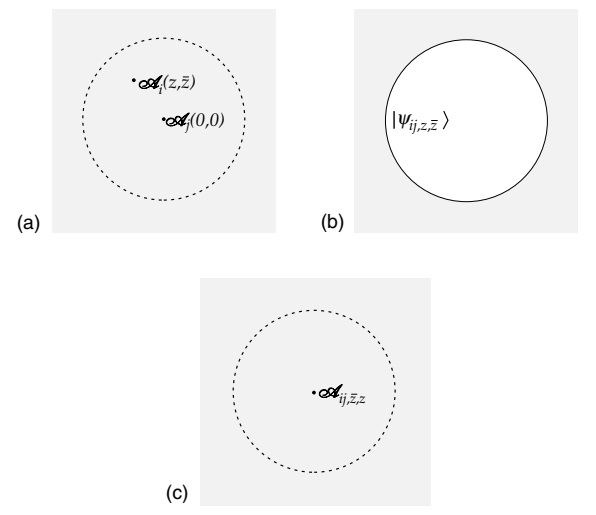
\includegraphics[width=0.8\textwidth,natwidth=370,natheight=300]{Fig2.7.jpg}\\
\caption{(a) World-sheet with two local operators. (b) Integration over fields on the interior of the disk produces boundary state $\left|\psi_{i j, z, \bar{z}}\right\rangle$. (c) Sewing in a disk with the corresponding local operator. Expanding in operators of definite weight gives the OPE.}\label{Fig2.7}
	\end{center}
\end{figure}
考察乘积
\begin{equation}
\mathscr{A}_{i}(z, \bar{z}) \mathscr{A}_{j}(0,0)
\end{equation}
其中$|z|<1$. 我么可以将路径积分分成对单位圆内部场$\phi_i$的积分, 对单位圆上场$\phi_b$的积分,对单位圆外部场$\phi_e$的积分. 正如上节末尾所讨论的,对$\phi_i$的积分给出$\phi_b$的某个泛函,称其为$\Psi_{i j, z, \bar{z}}\left[\phi_{\mathrm{b}}\right]$. 通过态-算符对应,这等价于将圆盘与合适的算符$\mathscr{A}$ 粘在一起. 为了将其变成以$L_{0}, \tilde{L}_{0}$本征态完备集做展开的标准形式
\begin{equation}
\mathscr{A}_{i j, z, \bar{z}}=\sum_{k} z^{h_{k}-h_{i}-h_{j}}-\tilde{h}_{k}-\tilde{h}_{i}-\tilde{h}_{j} c_{i j}^{k} \mathscr{A}_{k}
\end{equation}
其中z相关性与$\bar{z}$相关性像(\ref{2.4.20})中那样由共形权重决定. OPE的收敛性正是量子力学中一个完备集的收敛性. 只要在$\left|z^{\prime}\right| \leq|z|$中没有其他算符,这个构建就是可能的. 使得我们可以剪出半径$|z|+\epsilon$ 的圆.\\
对于三个算符
\begin{equation}
\mathscr{A}_{i}(0,0) \mathscr{A}_{j}(1,1) \mathscr{A}_{k}(z, \bar{z})
\end{equation}
$z\to 0$收敛区域$|z|<1$与$z\to 1$收敛区域$|1-z|<1$重叠. 那么三重积中$\mathscr{A}_l$ 的系数可以写成包含$c_{i k}^{l} c^{m} _{l j}$ 的求和或包含$c_{j k}^{l} c^{m} _{li}$ 的求和. 结合性要求这些和相等. 图解表示见(\ref{Fig2.8}).
\begin{figure}
	\begin{center}
		%	\includegraphics[width=0.8\textwidth,bb=0 0 490 192]{Fig2.3ClosedStringCoordinates.jpg}\\
		%1px=0.75pt
		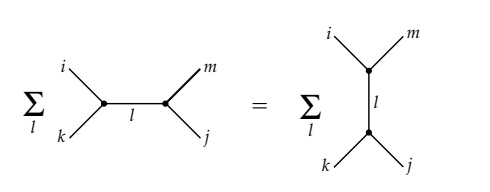
\includegraphics[width=0.8\textwidth,natwidth=300,natheight=110]{Fig2.8.jpg}\\
		\caption{Schematic picture of OPE associativity}\label{Fig2.8}
	\end{center}
\end{figure}
\centerline{\Large Virasoro代数和最高权重态}
现在对Virasoro生成元考察图(\ref{Fig2.6})的讨论:
\begin{equation}
\begin{aligned}
L_{m}|\mathscr{A}\rangle & \cong \oint \frac{d z}{2 \pi i} z^{m+1} T(z) \mathscr{A}(0,0) \\
& \cong L_{m} \cdot \mathscr{A}(0,0)
\end{aligned}
\end{equation}
这里我们进入了新的记法与概念. 给定态-算符同构,作用在Hilbert空间上的每一算符有一个作用在定域算符空间上的像. 换句话说,构成了围绕算符的相应围道并利用OPE计算出所导致的定域算符. 对应将态映射到态的$L_m$是将定域算符映射到定域算符的$L_m$. 一般而言,在不同位置$z_i$处会有定域算符. 对于每一个位置将有一个Virasoro代数的不同版本. 这些不同版本是以算符位置为中心的Laurent展开获得的. 在某些几何中也会存在生成元的一个标准基. 例如对于圆柱以z=0为中心的展开. “·”充当一个提醒:我们所讨论的是围绕特定算符的Laurent展开. \\
在这个记法下,$T\mathscr{A}$OPE是
\begin{equation}\label{2.9.5}
T(z) \mathscr{A}(0,0)=\sum_{m=-\infty}^{\infty} z^{-m-2} L_{m} \cdot \mathscr{A}(0,0)
\end{equation}
为了关联到早期记号(\ref{2.4.11})上,对于$n \geq 0$,$\mathscr{A}^{(n)}=L_{n-1} \cdot \mathscr{A}$ 以及$\mathscr{A}$的共形变换
\begin{equation}
\delta \mathscr{A}(z, \bar{z})=-\epsilon \sum_{n=0}^{\infty} \frac{1}{n !}\left[\partial^{n} v(z) L_{n-1}+\left(\partial^{n} v(z)\right)^{*} \tilde{L}_{n-1}\right] \cdot \mathscr{A}(z, \bar{z})
\end{equation}
利用$T\mathscr{A}$OPE的普遍形式(\ref{2.4.14}),我们有非常有用的结果
\begin{subequations}\label{2.9.7}
\begin{equation}
L_{-1} \cdot \mathscr{A}=\partial \mathscr{A}, \quad \tilde{L}_{-1} \cdot \mathscr{A}=\bar{\partial} \mathscr{A}
\end{equation}
\begin{equation}
L_{0} \cdot \mathscr{A}=h \mathscr{A}, \quad \tilde{L}_{0} \cdot \mathscr{A}=\tilde{h} \mathscr{A}
\end{equation}
\end{subequations}
OPE(\ref{2.9.5})暗示了权重为 $(h, \tilde{h})$的基本场$\mathcal{O}$. 其对应的态满足
\begin{subequations}
\begin{equation}
L_{0}|\mathcal{O}\rangle=h|\mathcal{O}\rangle, \quad \tilde{L}_{0}|\mathcal{O}\rangle=\tilde{h}|\mathcal{O}\rangle
\end{equation}
\begin{equation}
L_{m}|\mathcal{O}\rangle=\tilde{L}_{m}|\mathcal{O}\rangle=0, \quad m>0
\end{equation}
\end{subequations}
这样的态被称为最高权重态. 通过在任意态上重复作用下降算符,我们得到一个态,这个态被进一步的下降算符湮灭,称为最高权重态. \\
一个有趣的特殊情况是单位算符,算符乘积$T1$是非奇异的,所以在任意CFT中得到
\begin{equation}
L_{m}|1\rangle=\tilde{L}_{m}|1\rangle=0, \quad m \geq-1
\end{equation}
正如2.4节所标记的,算符$L_{0}$ 和 $L_{\pm 1}$构成闭代数,$\tilde{L}_{0}$ 和 $\tilde{L}_{\pm 1}$也如此. 全代数是
\begin{equation}
S L(2, \mathbf{C})
\end{equation}
因此$|1\rangle$也称为 $\operatorname{SL}(2, \mathbf{C})$-不变态. 它是唯一一个这样的态. 这是因为(\ref{2.9.7})暗示了对应任何 $\operatorname{SL}(2, \mathbf{C})$-不变态的算符$\mathscr{A}$独立于位置. 那么它必须是c数,正如(\ref{2.4.24}) 之后所解释的. 

\centerline{\Large 幺正CFT}
最高权重态在弦论以及Virasoro代数的表示论中扮演了重要的角色. 现在我们要导出几个在幺正CFT中成立的重要且普遍结果. 幺正CFT有正定内积,这使得
\begin{equation}
L_{m}^{\dagger}=L_{-m}, \quad \tilde{L}_{m}^{\dagger}=\tilde{L}_{-m}
\end{equation}
回忆:内积经由$\langle\alpha \mid A \beta\rangle=\left\langle A^{\dagger} \alpha \mid \beta\right\rangle$ 定义了伴随(adjoint) . 例如$X^\mu$CFT对于类空的$\mu$是幺正的. 如果我们对于基态取内积
\begin{equation}
\left\langle 0 ; k \mid 0 ; k^{\prime}\right\rangle=2 \pi \delta\left(k-k^{\prime}\right)
\end{equation}
并定义
\begin{equation}
\alpha_{m}^{\dagger}=\alpha_{-m}, \quad \tilde{\alpha}_{m}^{\dagger}=\tilde{\alpha}_{-m}
\end{equation}
这隐含地定义了所有更高态的内积. 这个CFT对于$X^\mu=0$不是幺正的,这是因为那里的对易关系存在一个负号. \\
第一个约束是幺正CFT中的任何态都必须有$h, \tilde{h} \geq 0$. 如果这对于最高权重态成立,那么对所有态成立. 对于最高权重态,Virasoro代数给出
\begin{equation}\label{2.9.14}
2 h_{\mathcal{O}}\langle\mathcal{O} \mid \mathcal{O}\rangle=2\left\langle\mathcal{O}\left|L_{0}\right| \mathcal{O}\right\rangle=\left\langle\mathcal{O}\left|\left[L_{1}, L_{-1}\right]\right| \mathcal{O}\right\rangle=\| L_{-1}|\mathcal{O}\rangle \|^{2} \geq 0
\end{equation}
所以$h_{\mathcal{O}} \geq 0 $. 如果 $h_{\mathcal{O}}=\tilde{h}_{\mathcal{O}}=0$,那么得出
\begin{equation}
L_{-1} \cdot \mathcal{O}=\tilde{L}_{-1} \cdot \mathcal{O}=0
\end{equation}
因而 $\mathcal{O}$是独立于位置的. 正如之前所标注的, $\mathcal{O}$必须是c数,即在幺正CFT中单位算符是唯一(0,0)算符. 惊奇的是,$X^\mu$是唯一的例外:相对应的态$x^{\mu}|0 ; 0\rangle$ 由于 $X^\mu$的无限范围是不归一的,并且方程(\ref{2.9.14}) 不再成立. 对于对应紧致维的CFT,一般定理是最有用的,这类例外不可能发生.\\
以同样的方式,在幺正CFT中,当且仅当$\tilde{h}=0$算符是全纯的,当且仅当h=0算符是反全纯的. 这是一个重要结果,我们重复如下:
\begin{equation}
\partial \mathscr{A}=0 \Leftrightarrow h=0, \quad \bar{\partial} \mathscr{A}=0 \Leftrightarrow \tilde{h}=0
\end{equation}
最后,利用之上讨论以及对易子$\left[L_{n}, L_{-n}\right]$,可以证明在幺正CFT中$c, \tilde{c} \geq 0$. 实际上,c=0的唯一幺正CFT是平庸的$L_n$. 

\centerline{\Large 零点能}
态-算符映射给出了另一种不同正规序列常数的简单推导. 在任何CFT中,我们知道$L_{0}|1\rangle=0$ 这决定了$L_0$ 的又一归一化.
在$X$CFT中,$|1\rangle=0$是基态,所以$a^x=0$. 在bc理论中,$|1\rangle=0$是激发态$b_{-1}|\downarrow\rangle$,所以为了与早期$\lambda=2$的结果(\ref{2.7.1}) 一致, $|\downarrow\rangle$的权重是-1.\\
这也提供了中心荷的物理解释. 在幺正CFT中,基态是$L_{0}=\tilde{L}_{0}=0$的$|1\rangle$. 径向生成元与时间平移生成元之间的共形变换(\ref{2.6.10})暗示了. 对于基态
\begin{equation}
E=-\frac{c+\tilde{c}}{24}
\end{equation}
这是Casimir能量,源于系统的有限尺度,且依赖于中心荷. 在量纲背景下,这个能量反比于系统的尺寸$l$,在这里是$2\pi$. 所以一般结果是
\begin{equation}
E=-\frac{\pi(c+\tilde{c})}{12 \ell}
\end{equation}
我们现在有三种计算正规序列常数的方式:
\begin{enumerate}
	\item 像(\ref{2.7.8})中那样,从Virasoro代数出发;
	\item 通过像(\ref{2.7.11})中那样,将正规序列的两种形式关联起来;
	\item 从之上的态-算符映射出发.
\end{enumerate}
然而把零点能加起来的方法是直观的,所以我们给出一种描述,且可以被更加忠实的方法检验:\\
1.对于每个Boson模,零点能为$\frac{1}{2} \omega$;对于每个Fermion模,零点能为$-\frac{1}{2} \omega$. 将能量加起来.\\
2.遇见形式为$\sum_{n=1}^{\infty}(n-\theta)$的发散和, $\theta$  源于非平庸的周期条件,定义其为
\begin{equation}
\sum_{n=1}^{\infty}(n-\theta)=\frac{1}{24}-\frac{1}{8}(2 \theta-1)^{2}
\end{equation}
这一值可以像(1.3.32)中那样,通过正规化并抛弃掉平方发散部分获得.\\
3.之上给出了w参考系生成元$T_0$的正规序列常数,$T_0$由(\ref{2.6.8})给出. 对于$L_0$我们必须加上非张量修正$\frac{1}{24} c$. \\
对于自由Boson场,模是整数值,所以在第2步之后,对于$\theta=0$ ,我们得到了求和的一半,其是$-\frac{1}{24} $. 这恰好被第3步的修正抵消,给出$a^x=0$. 对于鬼场,我们类似地得到$\frac{2}{24}-\frac{26}{24}=-1$.

% \setcounter{section}{0}%更改chapter的计数器值
% %\numberwithin{equation}{chapter}%公式计数器从属于节计数器
% \numberwithin{equation}{section}%公式计数器从属于节计数器
% %\numberwithin{figure}{section}%图计数器从属于节计数器
% \setcounter{chapter}{2}

\chapter{\texorpdfstring{Polyakov路径积分}{3 The Polyakov path integral}} \label{cha:3}

我们现在用 Polyakov 路径积分和共形场论对弦论做一系统研究. 在介绍路径积分的图像后, 我们讨论规范固定, Weyl 反常与顶点算符, 
之后我们将弦论推广至弯曲时空.

\section{\texorpdfstring{世界面上的求和}{3.1 Sums over world-sheets}} \label{sec:3.2}
Feynman 路径积分是表示量子论的一种方法, 并且它是描述弦论相互作用的一个非常自然的方法. 在路径积分量子化中, 振幅通过对初态和末态之间所有可能的历史求和获得. 每个历史被赋予权重
\begin{equation}
	\exp (\mi S_{\mathrm{cl}} / \hbar) \:, \label{3.1.1}
\end{equation}
其中$S_{\mathrm{cl}}$是给定历史的经典作用量. 因此, 对连接给定初始曲线与终末曲线的所有世界面求和将定义弦论中的振幅. 图\ref{Fig3.1}a 针对开弦, 图\ref{Fig3.1}b 针对闭弦. 对相对论点粒子的类似求和产生自由传播子.
\vspace{-0.5cm}
\begin{figure}[h]
	\begin{center}
		%width=0.8\textwidth,bb=0 0 680 374
		%1px=0.75pt
		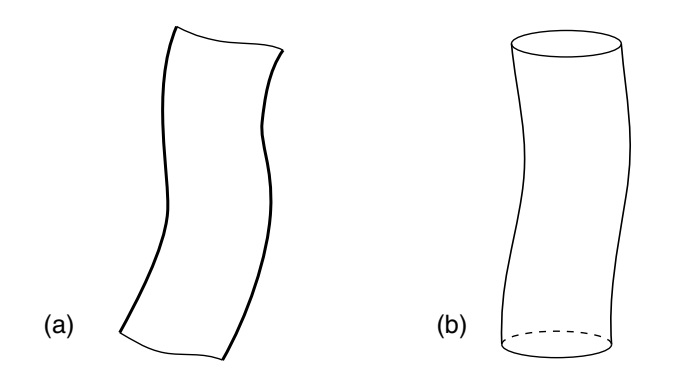
\includegraphics[width=0.8\textwidth,natwidth=500,natheight=240]{Fig3.1.jpg}
\caption{(a) 拓扑为长带的的开弦世界面. 粗曲线是弦端点的世界线. (b) 拓扑为圆柱的闭弦世界面.}\label{Fig3.1}
	\end{center}
\end{figure}

可以想象出弦产生相互作用的数个方法. 一种是连接相互作用, 两弦相交时的能量; 另一种是经由某种量子场的长程力. 然而, 我们在弦论中增加的相互作用不可能与对称性相容; 稍后我们将看到其中的原因. 与之相反, 唯一允许的相互作用已经隐含在世界面求和中. 例如考察图\ref{Fig3.2} 所示的世界面. 图\ref{Fig3.2}a看起来是对图\ref{Fig3.1}a中的开弦振幅的量子修正. 这个修正中包含一个有两个开弦的中间态. 图\ref{Fig3.2}b有三个外闭弦, 它代表一个弦衰变成两个弦. 从中看出这是在弦中引入相互作用的一种正确方式. 我们将看到这些相互作用产生了包含引力的相容理论, 它们有限且幺正.
\begin{figure}[h]
	\begin{center}
		%width=0.8\textwidth,bb=0 0 741 390
		%1px=0.75pt
		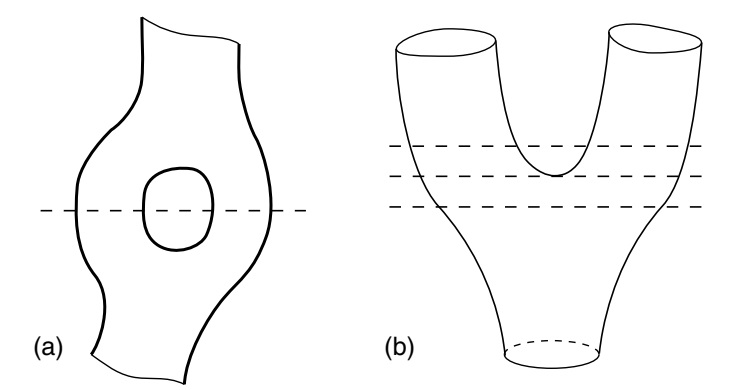
\includegraphics[width=0.75\textwidth,natwidth=500,natheight=218]{Fig3.2.jpg}\\
\caption{(a)开弦传播子的量子修正. (b) 一个闭弦衰变到两个闭弦. 虚线代表时间切片.}\label{Fig3.2}
	\end{center}
\end{figure}

像图\ref{Fig3.3}那样在连续的几个时刻里考察图\ref{Fig3.2}b的过程是很有趣的.
\begin{figure}
	\begin{center}
		%width=0.8\textwidth,bb=0 0 510 279
		%1px=0.75pt
		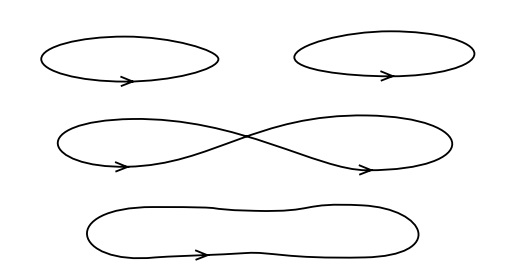
\includegraphics[width=0.65\textwidth,natwidth=350,natheight=138]{Fig3.3.jpg}\\
\caption{图\ref{Fig3.2}(b)中的数个连续切面. 箭头指明了弦的定向.}\label{Fig3.3}
	\end{center}
\end{figure}
在闭弦理论中, 所有粒子作为弦的不同激发态获得. 而所有的相互作用(规范, 引力, Yukawa)源于图\ref{Fig3.3}的单个过程. 对于有开弦的理论, 存在几种额外可能发生的过程, 如图\ref{fig:3.4}所示. 在一给定时刻, 图\ref{Fig3.3}与图\ref{fig:3.4}发生在确定的时空点, 但这是一个错觉. 一个不同的切面(slicing)将显然的相互作用放在不同点上; 在时空中不存在可区分的点. 相互作用仅源于世界面的整体拓扑, 而世界面的定域性质在自由情况下是相同的. 正如导论中所讨论的, 这一点涂抹出来的相互作用截断了引力的短程发散. 
\vspace{0.5cm}
\begin{figure}[h]
	\begin{center}
		%width=0.8\textwidth,bb=0 0 783 471
		%1px=0.75pt
		\includegraphics[width=0.7\textwidth,natwidth=520,natheight=250]{fig:3.4.jpg}\\
\caption{包含开弦的过程: (a) 开弦 $\leftrightarrow$ 开弦 $+$ 开弦; (b) 闭弦 $\leftrightarrow$ 开弦; (c) 开弦 $+$ 开弦 $\leftrightarrow$ 开弦 $+$ 开弦; (d) 开弦 $\leftrightarrow$ 开弦 $+$ 闭弦.}\label{fig:3.4}
	\end{center}
\end{figure}

实际上还有几种不同的弦论, 依赖于我们在世界面求和中引入的拓扑. 注意到我们所画的世界面有两类边界, 源边界对应初态与末态的弦构型, 而端点边界对应开弦端点的世界线. 现在忽视源边界; 我们将在本章后面讨论源的细节. 所以在之后的讨论中, “边界”意味着端点边界. 那么有4种方式定义对世界面求和, 对应1.4节末尾所列的4种自由弦理论:
\begin{enumerate}
	\item 闭定向: 所有无边界的定向世界面; 
	\item 闭非定向: 所有无边界的世界面; 
	\item 闭加开定向: 有任意个边界的所有定向世界面; 
	\item 闭加开非定向: 有任意个边界的所有世界面; 
\end{enumerate} 


\begin{figure}[h]
	\begin{center}
		%width=0.8\textwidth,bb=0 0 717 409
		%1px=0.75pt
		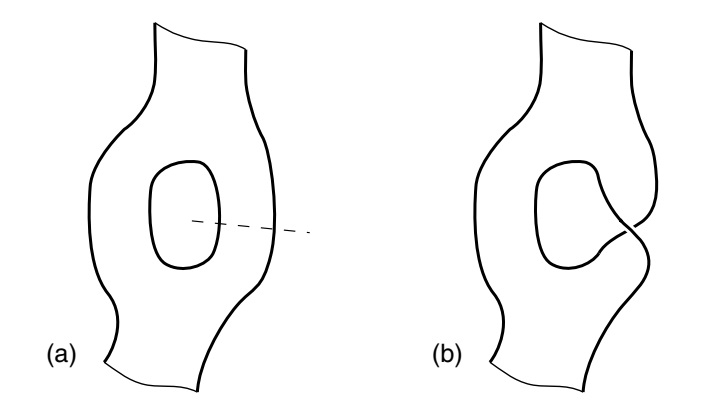
\includegraphics[width=0.65\textwidth,natwidth=500,natheight=230]{Fig3.5.jpg}\\
\caption{2-开弦振幅的定向贡献(a)和非定向贡献(b).}\label{Fig3.5}
	\end{center}
\end{figure}

我们在这里要详述两件事. 其一是非定向世界面内含物之间的连结以及1.4节所描述的$\Omega=+1$投影. 图\ref{Fig3.5}展示了计入开弦非定向理论的两个世界面. 图\ref{Fig3.5}(b)的世界面等价于沿着虚线剪断图\ref{Fig3.5}(a)的定向世界面. 我们用$0 \leq \sigma \leq \pi$参量化它, 并要求在剪断处的场满足
\begin{equation}
X_{\text {upper }}^{\mu}(\sigma)=X_{\text {lower }}^{\mu}(\pi-\sigma) \:. \label{3.1.2}
\end{equation}
这反过来等价于用算符$\Omega$作用在开弦态上. 将这两个平面赋予合适的权重加起来, 那么相当于插入算符$\frac{1}{2}(1+\Omega)$, 其投射到
$\Omega=+1$的态上. 在对所有定向曲面与非定向曲面的求和中, 在所有中间态上插入投影算符, 将频谱约化至$\Omega=+1$部分.

\begin{figure}[h]
	\begin{center}
		%width=0.8\textwidth,bb=0 0 740 280
		%1px=0.75pt
		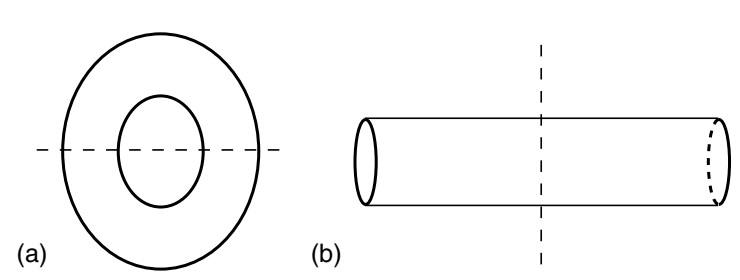
\includegraphics[width=0.8\textwidth,natwidth=520,natheight=190]{Fig3.6.jpg}\\
\caption{(a) 圆环: 中间态是两个开弦. (b) 具有相同拓扑的圆柱: 中间态是一个闭弦.}\label{Fig3.6}
	\end{center}
\end{figure}

其二, 之上的列表中没有计入只有开弦的理论. 我们来细致地解释下为什么是这种情况.
考察一个拓扑为圆环的世界面, 如图\ref{Fig3.6}(a). 方便起见, 我们只画出了真空振幅, 但通过连上合适的源, 相同的讨论也适用于散射振幅. 从虚线中可以看出这是一个中间态有两个开弦的过程. 因而这类拓扑的世界面必须出现在有开弦的任何理论中. 在图\ref{Fig3.6}(b), 我们将同一拓扑画成圆柱, 并在单个闭弦的中间态上切开它. 因此, 即使我们只从闭弦出发, 对世界面的求和将必然地引入这样的过程——开弦的散射产生闭弦. 随着振幅的发散, 我们将细致地看到它是如何运作的.

开弦理论中闭弦的需求可以从另一方面看到. 考察图\ref{fig:3.4} (a)和(b)中的相互作用, 但时间反演: 两个开弦合并成一个, 一个开弦变成闭弦. 在相互作用点附加它们是相同的, 两个端点合并为了有第一个相互作用而没有第二个. 将要求在弦的动力学上附加某些非定域约束; 这将确认是不相容的. 可以对图\ref{fig:3.4}(c)和(d)作同一讨论, 其中相互作用定域的是一对弦的重新连接, 因而, 如果任何开弦相互作用被允许了, 那么在开弦产生闭弦的同一过程也是允许的.

\section{\texorpdfstring{Polyakov路径积分}{3.2 The Polyakov path integral}} \label{sec:3.2}

我们现在开始研究对世界面的求和, 它表示为对Polyakov形式体系的场积分. 我们这里与第1章有个区别: 闵可夫斯基 度规 $\gamma_{ab}$ 被替换为特征为$(+,+)$的 Euclid 度规$g_{a b}(\sigma^{1}, \sigma^{2})$. 积分取遍所有的 Euclid 度规以及世界面在 闵可夫斯基 时空中的嵌入$X^{\mu}(\sigma^{1}, \sigma^{2})$: 
\begin{equation}\label{3.2.1}
\int[\dif X \dif g] \exp (-S) \:.
\end{equation}
Euclid作用量是
\begin{equation}
S=S_{X}+\lambda \chi \:, \label{3.2.2}
\end{equation}
其中
\begin{subequations}\label{3.2.3}
\begin{align}
S_{X}&=\frac{1}{4 \pi \alpha^{\prime}} \int_{M} \dif^{2} \sigma \: g^{1 / 2} g^{a b} \partial_{a} X^{\mu} \partial_{b} X_{\mu} \:, \label{3.2.3a} \\
\chi&=\frac{1}{4 \pi} \int_{M} \dif^{2} \sigma \: g^{1 / 2} R+\frac{1}{2 \pi} \int_{\partial M} \dif s\: k \:. \label{3.2.3b}
\end{align}
\end{subequations}
这里$\dif s$是沿着边界的固有时, $k$是边界的测地线曲率 $k=\pm t^{a} n_{b} \nabla_{a} t^{b}$. \\
\begin{remark}
$t^a$ 是与边界相切的单位向量, 而$n^a$是指向外侧与$t^a$垂直的单位矢量, $+$号对应类时边界, $-$对应类空边界. 在这里边界总是类空的. 
\end{remark}

Euclid路径积分的优点是对度规的积分可以更好地定义. 我们所描述的拓扑非平庸世界面可以有非奇异的Euclid度规, 而闵可夫斯基度规不行. 我们将取Euclid理论(\ref{3.2.1})作为出发点. 我们将展示如何给它一个精准的定义并且它定义了相容时空理论. 然而, 我们将给出一个简要的形式讨论, 它等价于我们出发点闵可夫斯基理论. 

我们从点粒子的例子出发, 其中路径积分
\begin{equation}
\int[\dif \eta \, \dif X] \exp \left[\frac{\mi}{2} \int \dif \tau\: \Bigl(\eta^{-1} \dot{X}^{\mu} \dot{X}_{\mu}-\eta m^{2}\Bigr)\right] \label{3.2.4}
\end{equation}
是振荡的. 对$\eta, X^\mu$ 的路径积分是普通积分的乘积, 因而我们可以像普通积分那样对围道变形. 如果我们取
\begin{equation}
\eta(\tau) \rightarrow e^{-i \theta} \eta(\tau)\:, \quad X^{0}(\tau) \rightarrow e^{-i \theta} X^{0}(\tau) \:, \label{3.2.5}
\end{equation}
对于无限小的$\theta$, 指数中的所有项要求有一负的实部, 使其收敛. 现在我们可以在场空间中旋转围道$\eta=-\mi e, X^{0}=-\mi X^{D}$ , 积分变成
\begin{equation}
\int[\dif e \, \dif X] \exp \Biggl[-\frac{1}{2} \int \dif \tau \: \Biggl(e^{-1} \sum_{\mu=1}^{D} \dot{X}^{\mu} \dot{X}^{\mu}+e m^{2}\Biggr)\Biggr] \:. \label{3.2.6}
\end{equation}
这是路径积分(\ref{3.2.1})的Euclid点粒子类比. 我们仅仅做了一个围道旋转, 所以Euclid路径积分给出与闵可夫斯基相同的振幅. 

如果我们将度规写成四元基的形式$\gamma_{a b}=-e_{a}^{0} e_{b}^{0}+e_{a}^{1} e_{b}^{1}$, 并在$e_a^0$上做同一旋转, 那么相同的处理适用于Polyakov作用量. 
这提供了闵可夫斯基路径积分与Euclid路径积分等效的一个形式证明. 通过显式的计算, 在光锥规范和共形规范下分别证明了它们有相同的振幅.
在(\ref{3.2.3a})中我们留下了$X^0$的旋转, 这是为了强调时空的闵可夫斯基特性. 写成了$X^0$的形式, 运动方程与OPE是协变的, 度规为$\eta^{\mu\nu}$. 

我们注意到在二维中, $\chi$定域地是全导数, 因而反依赖于世界面的拓扑——它是世界面的Euler数. 因而, $\me^{-\lambda \chi}$因子在路径积分中只影响世界面求和中不同拓扑的相对权重. 如果我们向世界面中增加额外的带, 就像我们从图\ref{Fig3.1}a到图\ref{Fig3.2}a中做的那样, Euler数减1, 路径积分被赋予额外的权重$\me^\lambda$. 由于增加一个带对应于发射并再吸收一个虚开弦, 从任意过程中发射一个开弦的振幅正比于$\me^{\lambda/2}$. 在任意世界面上增加一个把手将Euler数减2, 因而增加因子$\me^{2\lambda}$.  由于这对应发射和再吸收一个闭弦, 发射一个闭弦的振幅正比于$\me^\lambda$. 作用量中的Euler项因而控制着弦论中的耦合常数, 其中
\begin{equation}\label{3.2.7}
g_{\mathrm{o}}^{2} \sim g_{\mathrm{c}} \sim \me^{\lambda} \:.
\end{equation}
附带的, $\lambda$可以视为理论中的自由参量, 这与绪论中弦论没有这种参量的陈述矛盾. 这是一个关键点, 我们将在\ref{sec:3.7}节解决它.

另一方面, 耦合的计数以一种简单的方式扩张到有弦源的世界面. 闭弦的源是封闭的圈, 开弦的源是有边界的线段. 方便起见, 我们将要求开弦源边界与端点边界在是世界面度规下成直角. 我们必须小心, 因为边界曲率在角处发散: Euler数是
\begin{equation}
\chi=\tilde{\chi}+\frac{1}{4} n_{\mathrm{c}} \:, \label{3.2.8}
\end{equation}
其中 仅包括光滑边界部分上的积分. $n_\mathrm{c}$是角的数目. 路径积分正确的权重是
\begin{equation}\label{3.2.9}
\exp (-\lambda \tilde{\chi})=\exp (-\lambda \chi+\lambda n_{\mathrm{c}} / 4) \:. 
\end{equation}
这源于幺正性: 如果我们剪开世界面, $\lambda$相关性必须不变. 对于权重(\ref{3.2.9})正是这种情况,
这是因为在$\tilde{\chi}$中的面积分在边缘处抵消了. 增加一个闭弦源相当于在世界面上剪了个洞, 并将$\chi$减1. 
增加开弦源使$\chi$不变但$n_c$加2. 因而, 我们得到了发射闭弦或开弦的振幅, 与\eqref{3.2.7}相同. 

\section{\texorpdfstring{规范固定}{3.3 Gauge fixing}} \label{sec:3.3}

路径积分\eqref{3.2.1}不是完全正确的, 它包含一个庞大的重复计数. 这是因为构型$(X, g)$与 $(X^{\prime}, g^{\prime})$若通过diff $\times$ Weyl对称性相关, 则它们代表同一物理构型. 事实上, 我们需要除以定域对称群的体积,
\begin{equation}\label{3.3.1}
\int \frac{[\dif X\, \dif g]}{V_{\text {diff } \times \text { Weyl }}} \exp (-S) \equiv Z \:.
\end{equation}
我们将通过规范固定实现这一点, 对穿过每一规范等价类一个切片积分, 并通过 Faddeev--Popov 方法获得切片上的正确测度.


在第\ref{cha:1}章, 我们附加了光锥规范.  这由于某些目的是有用的, 但隐藏了理论的某些对称性, 所以我们现在做另一选择. 注意到度规是对称的, 有三个独立分量, 并存在三个规范函数, 两个坐标与度规的定域缩放. 因此恰好存在足够多的规范自由度以消除度规上的积分, 将其固定在某个特定的泛函形式, 我们称其为基准度规
\begin{equation}
g_{a b}(\sigma) \rightarrow \hat{g}_{a b}(\sigma) \:. \label{3.3.2}
\end{equation}
一个简单的选择是平坦度规或\emph{单位规范}度规
\begin{equation}\label{3.3.3}
\hat{g}_{a b}(\sigma)=\delta_{a b} \:. 
\end{equation}
有时希望单独考虑diff群的效应. 我们可以将任意度规变成单位形式的一个Weyl变换. 这是\emph{共形规范}
\begin{equation}
\hat{g}_{a b}(\sigma)=\exp [2 \omega(\sigma)] \delta_{a b} \:. \label{3.3.4}
\end{equation}

这样, 任何度规至少可以定域地变成平坦形式. 首先, 做一Weyl变换以使里奇标量为零. 里奇标量的Weyl变换
\begin{equation}\label{3.3.5}
g^{\prime 1 / 2} R^{\prime}=g^{1 / 2}\left(R-2 \nabla^{2} \omega\right) \:.
\end{equation}
令$R^{\prime}=0$ 要求解 $2 \nabla^{2} \omega=R$. 这总是可能的, 类似于静电学中的讨论. 在二维中, 里奇标量为零暗示着黎曼张量为零, 这是因为黎曼张量的对称性暗示
\begin{equation}
R_{a b c d}=\frac{1}{2}(g_{a c} g_{b d}-g_{a d} g_{b c}) R  \:. \label{3.3.6}
\end{equation}
所以度规是平坦的, 且坐标等价于单位度规(\ref{3.2.3}).

在这里像第\ref{cha:2}章中那样引入复坐标$z=\sigma^{1}+\mi \sigma^{2}$, 平坦度规$\dif s^{2}=\dif z \dif \bar{z}$. 考察一个坐标变换, 使得$z^\prime$是z的全纯函数
\begin{equation}\label{3.3.7}
z^{\prime} \equiv \sigma^{\prime 1}+\mi \sigma^{\prime 2}=f(z) \:, 
\end{equation}
结合一个Weyl变换. 新度规是
\begin{equation}
\dif s^{\prime 2}=\exp (2 \omega)\lvert\partial_{z} f\rvert^{-2} \dif z^{\prime} \dif \bar{z}^{\prime} \:. \label{3.3.8}
\end{equation}
那么对于
\begin{equation}\label{3.3.9}
\omega=\ln \lvert\partial_{z} f\rvert \:,
\end{equation}
这个度规是不变的. %因而, 我们还存在一个额外的自由度. diff$\:\times\:$Weyl变换.


当我们考察整个世界面时, 这种额外自由度大多会被消除. 这里存在两个问题. 其一, 在Noether定理和Ward恒等式的讨论中, 我们在\eqref{2.3.10}下面仔细强调了这些结果依赖于定域定义在世界面上的对称性. 变换(\ref{3.3.7})和(\ref{3.3.9})因而会给出守恒流与Ward等式. 这是第\ref{cha:2}章研究的共形不变性. 我们看到这源于保持单位度规不变的 diff$\:\times\:$Weyl子群.

第二个问题是当我们确实考察全世界面时, 我们对度规和规范自由度的计数发生了什么. 我们将在第\ref{cha:5}章考虑它们.

\subsection*{Faddeev-Popov行列式}

在固定度规之后, 泛函积分取遍由$X^\mu$参量化的切片. 为了获得正确的测度, 我们使用Faddeev-Popov手续. 这个方法与杨-米尔斯理论中获得规范固定测度的方法相同. 图\ref{Fig:3.7}阐明了这个方法.
\begin{figure}
	\begin{center}
		%width=0.8\textwidth,bb=0 0 654 372
		%1px=0.75pt
		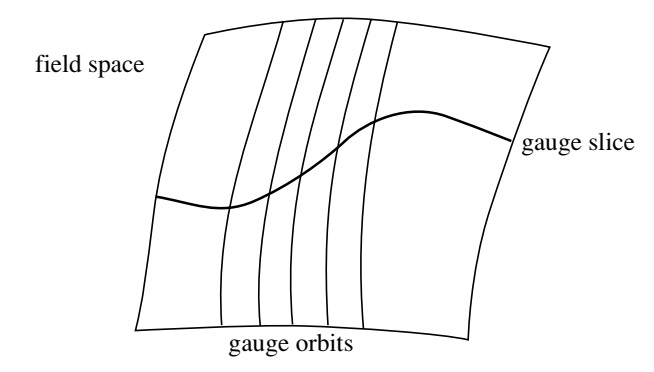
\includegraphics[width=0.8\textwidth,natwidth=490,natheight=279]{Fig3.7.jpg}\\
\caption{Faddeev–Popov手续的图形表示. 规范轨道是规范等价构型的族. 对整个场空间积分并除以轨道体积等价于在一个与所有轨道都相交一次的切片上积分.}\label{Fig:3.7}
	\end{center}
\end{figure}


令$\zeta$ 为坐标变换与Weyl变换的组合
\begin{equation}
\zeta: g \rightarrow g^{\zeta}, \quad g_{a b}^{\zeta}(\sigma^{\prime}) = 
\exp [2 \omega(\sigma)] \frac{\partial \sigma^{c}}{\partial \sigma^{\prime a}} \frac{\partial \sigma^{d}}{\partial \sigma^{b}} g_{c d}(\sigma) \:. \label{3.3.10}
\end{equation}
根据标准程序, 定义Faddeev-Popov测度$\Delta_{\mathrm{FP}}$
\begin{equation}\label{3.3.11}
1=\Delta_{\mathrm{FP}}(g) \int[\dif \zeta] \: \delta(g-\hat{g}^{\zeta}) \:, 
\end{equation}
其中$\hat{g}_{a b}$ 是基准度规. 在(\ref{3.3.11})中, $[\dif \zeta]$是diff $\times$ Weyl群上的规范不变测度. $\delta$-函数实际上是 $\delta$-泛函, 
要求在每一点$g_{a b}(\sigma)=\hat{g}_{a b}^{\zeta}(\sigma)$. 

将(\ref{3.3.11})代入泛函积分(\ref{3.3.1})
\begin{equation}
Z[\hat{g}]=\int \frac{[\dif \zeta \,\dif X \,\dif g]}{V_{\text {diff } \times \text { Weyl }}}  \Delta_{\mathrm{FP}}(g) \delta(g-\hat{g}^{\zeta}) \exp (-S[X, g]) \:. \label{3.3.12}
\end{equation}
进行对$g_{ab}$的积分, 并重新命名积分变量$X \to X^{\zeta}$, 得到
\begin{equation}
Z[\hat{g}]=\int \frac{[\dif \zeta\, \dif X^{\zeta}]}{V_{\text {diff } \times \text { Weyl }}} \Delta_{\mathrm{FP}}(\hat{g}^{\zeta}) \exp (-S[X^{\zeta}, \hat{g}^{\zeta}]) \:. \label{3.3.13}
\end{equation}
现在利用$\Delta_{\mathrm{FP}}$的规范不变性\footnote{$\Delta_{\mathrm{FP}}$的规范不变性: 
\begin{align*}
\Delta_{\mathrm{FP}}(g^{\zeta})^{-1} &=\int[\dif \zeta^{\prime}] \: \delta(g^{\zeta}-\hat{g}^{\zeta^{\prime}})
=\int[\dif \zeta^{\prime}]\: \delta(g-\hat{g}^{\zeta^{-1} \cdot \zeta^{\prime}}) \\
&=\int[\dif \zeta^{\prime \prime}] \: \delta(g-\hat{g}^{\zeta^{\prime \prime}})=\Delta_{\mathrm{FP}}(g)^{-1} \:,
\end{align*}
其中$\zeta^{\prime \prime}=\zeta^{-1} \cdot \zeta^{\prime} $.}, 泛函积分测度$[\dif X]$的不变性, 以及作用量的规范不变性, 得: 
\begin{equation}
Z[\hat{g}]=\int \frac{[\dif \zeta\, \dif X]}{V_{\text {diff } \times \text { Weyl }}} \Delta_{\mathrm{FP}}(\hat{g}) \exp (-S[X, \hat{g}]) \:. \label{3.3.14}
\end{equation}
最后, 被积函数中没有什么量依赖于$\zeta$, 所以$\zeta$的积分仅产生了规范群的体积并与分母抵消, 留下
\begin{equation}
Z[\hat{g}]=\int[\dif X] \: \Delta_{\mathrm{FP}}(\hat{g}) \exp (-S[X, \hat{g}]) \:. \label{3.3.15}
\end{equation}
因而$\Delta_{\mathrm{FP}}(\hat{g})$ 是切片上的正确测度.

为了计算Faddeev-Popov测度的表达式(\ref{3.3.11}), 我们假定规范选择完美地固定了规范对称性, 使得对于精确的一个$\zeta$值, $\delta(g-\hat{g} ^\zeta)$非零; 而对于$\delta(g-\hat{g}^ \zeta)$这是一个等式. 正如前面提起的, 存在一个整体的小的错误匹配, 我们将在时间参与进来时处理它——它不影响世界面的定域性质. 对于接近于1的 $\zeta$, 我们可以展开
\begin{align}
\delta g_{a b} &=2 \delta \omega \,g_{a b}-\nabla_{a} \delta \sigma_{b}-\nabla_{b} \delta \sigma_{a} \nonumber \\
&=(2 \delta \omega-\nabla_{c} \delta \sigma^{c}) g_{a b}-2(P_{1} \delta \sigma)_{a b} \:. \label{3.3.16}
\end{align}
其中$P_1$是使矢量成为无迹对称2-张量的微分算符
\begin{equation}
(P_{1} \delta \sigma)_{a b}=\frac{1}{2}(\nabla_{a} \delta \sigma_{b}+\nabla_{b} \delta \sigma_{a}-g_{a b} \nabla_{c} \delta \sigma^{c}) \:. \label{3.3.17}
\end{equation}
在1附近, 逆行列式(\ref{3.3.11})变成
\begin{align}
&\Delta_{\mathrm{FP}}(\hat{g})^{-1} \nonumber \\
&\quad =\int[\dif \delta \omega \, \dif \delta \sigma]\: \delta\Bigl[-(2 \delta \omega-\hat{\nabla} \cdot \delta \sigma) \hat{g}+2 \hat{P}_{1} \delta \sigma\Bigr] \nonumber \\
&\quad =\int[\dif \delta \omega \, \dif \beta\, \dif \delta \sigma] \: \exp \biggl\{2 \pi \mi \int \dif^{2} \sigma \: \hat{g}^{1 / 2} \beta^{a b}
\Bigl[-(2 \delta \omega-\hat{\nabla} \cdot \delta \sigma) \hat{g}+2 \hat{P}_{1} \delta \sigma\Bigr]_{a b}\biggr\} \nonumber \\
&\quad =\int[\dif \beta^{\prime}\, \dif \delta \sigma]\: \exp \biggl\{4 \pi \mi \int \dif^{2} \sigma \: \hat{g}^{1 / 2} \beta^{\prime a b}
(\hat{P}_{1} \delta \sigma)_{a b}\biggr\} \:. \label{3.3.18}
\end{align}
微分算符上的帽子代表它包含基准度规$\hat{g}$. 在第二个等式中, 我们使用了泛函$\delta$函数的积分表示, 引入了对称张量场$\beta^{a b} $. 
在第三个等式中我们积掉了$\delta \omega$, 它产生了一个$\delta$-泛函迫使 $\beta^{a b}$无迹; 那么泛函积分$[\dif \beta^{\prime}]$是对\emph{无迹}对称张量积分. 
我们现在有了 $\Delta_{\mathrm{FP}}(\hat{g})^{-1}$ 作为对矢量场 $\delta \sigma^{a}$ 与无迹对称张量 $\beta^{\prime a b}$的泛函积分表示.

通过将玻色场替换为相应的Grassmann\emph{鬼}场
\begin{subequations} \label{3.3.19}
\begin{align}
\delta \sigma^{a} &\rightarrow c^{a} \:, \label{3.3.19a}\\
\beta_{a b}^{\prime} & \rightarrow b_{a b} \:, \label{3.3.19b}
\end{align}
\end{subequations}
我们可以转化路径积分, 其中$b^{a b}$像$\beta^{\prime a b}$一样是无迹的. 因而,
\begin{equation}
\Delta_{\mathrm{FP}}(\hat{g})=\int[\dif b\, \dif c] \: \exp (-S_{\mathrm{g}}) \:, \label{3.3.20}
\end{equation}
其中, 在场的一个方便的归一化下, 鬼场作用量是
\begin{equation}\label{3.3.21}
S_{\mathrm{g}}=\frac{1}{2 \pi} \int \dif^{2} \sigma \: \hat{g}^{1 / 2} b_{a b} \hat{\nabla}^{a} c^{b}=\frac{1}{2 \pi} \int \dif^{2} \sigma \hat{g}^{1 / 2} b_{a b}(\hat{P}_{1} c)^{a b} \:. 
\end{equation}
定域地在世界面上, Polyakov路径积分是
\begin{equation}\label{3.3.22}
Z[\hat{g}]=\int[\dif X\, \dif b\, \dif c]\: \exp (-S_{X}-S_{\mathrm{g}}) \:. 
\end{equation}
这个作用量是场的二次型, 所以我们可以以行列式的形式计算路径积分. 这个计算将在第\ref{cha:5}章进行更细致的描述; 这里的结果是
\begin{equation}
Z[\hat{g}]=(\operatorname{det} \hat{\nabla}^{2})^{-D / 2} \operatorname{det} \hat{P}_{1} \:, \label{3.3.23}
\end{equation}
第一个行列式来自于X积分, 而第二个来自于鬼场积分.

在共形规范下, $\hat{g}_{a b}(\sigma)=\exp [2 \omega(\sigma)] \delta_{a b}$, 鬼场作用量(\ref{3.3.21})是
\begin{align}
S_{\mathrm{g}} &=\frac{1}{2 \pi} \int \dif^{2} z\:\Bigl(b_{z z} \nabla_{\bar{z}} c^{z}+b_{\bar{z} \bar{z}} \nabla_{z} c^{\bar{z}}\Bigr)  \nonumber \\
&=\frac{1}{2 \pi} \int \dif^{2} z\:\Bigl(b_{z z} \partial_{\bar{z}} c^{z}+b_{\bar{z} \bar{z}} \partial_{z} c^{\bar{z}}\Bigr) \:. \label{3.3.24}
\end{align}
注意, $\omega(\sigma)$并没有出现在最终形式中.  这是因为若张量只有$z$指标, 那么它的协变$\bar{z}$导数将简化成简单导数, 反之亦然, 读者可以通过解出联络张量来验证这一点. 
由于作用量\eqref{3.3.24}是Weyl不变的, 所以$b_{a b}$ 和 $c^{a}$ 在左Weyl变换下是中性的($b^{a b}$和 $c_{a}$则相反, 它们包含额外的度规因子). 由于共形变换是坐标变换\eqref{3.3.7} 和Weyl变换\eqref{3.3.9}的组合, 我们可以立即从张量指标中读出 $b_{a b}$ 与 $c^{a}$ 的共形变换: 这是 $(h_{b}, h_{c})=(2,-1)$的$bc$ CFT 与 $(\tilde{h}_{b}, \tilde{h}_{c})=(2,-1)$的$\tilde{b} \tilde{c}$ CFT .

我们推导规范固定路径积分的方式有时被称为“启发”式推导. Polyakov泛函积分(\ref{3.3.1})由于庞大的规范重复计数不是合理定义的. 另一方面, 规范固定泛函(\ref{3.3.22})的定义是相当好的, 并可以清楚地计算出来. 由于实用的原因, 我们或许应该视规范固定的形式为出发点, 而规范不变的那个则给出了直观解释. 在规范固定形式中, 规范对称性的实质内容表示为BRST不变, 我们将在下一章着手处理. 

在开弦中, 我们也要考虑包含边界线段的部分. 将泛函积分视为固定区域上场的积分是方便的, 所以diff不变性被限制为使边界变换到自身的坐标变换. 因而变分$\delta \sigma^{a}$ 有一零法向分量
\begin{equation}
n_{a} \delta \sigma^{a}=0 \:. \label{3.3.25}
\end{equation}
这个边界条件被相应的鬼场
\begin{equation}
n_{a} c^{a}=0 \:, \label{3.3.26}
\end{equation}
所继承, 所以$c^{a}$正比于切向矢量$t^{a}$. 那么运动方程给$b_{a b}$提供了一个边界条件. 它们有表面项
\begin{equation}
\int_{\partial M} \dif s\: n^{a} b_{a b} \delta c^{b}=0 \:. \label{3.3.27}
\end{equation}
加上$c^a$上的边界条件. 这暗示了
\begin{equation}
n_{a} t_{b} b^{a b}=0 \:. \label{3.3.28}
\end{equation}
这些是我们在\ref{sec:2.7}节所用的边界条件.

\section{\texorpdfstring{Weyl反常}{3.4 The Weyl anomaly}} \label{sec:3.4}

弦论的关键特征之一仅在满足特定条件的时空背景下才是自洽的. 对于平坦时空中的玻色弦论, 条件是$D=26$. 
它首次是从散射振幅的一个病态中发现的. 在光锥分析中, 
它来自于 Lorentz 对称性的缺失. 这一约束的潜在原因是定域世界面对称性中的一个\emph{反常}. 在我们现在的体系中, 反常是在 Weyl 对称性中: $T^{a}{}_{a}$在经典的意义上为零, 
但在量子理论中不是. 

整体Weyl变换, $\omega(\sigma)=$ 常数, 等价于长度的总体缩放. 几个四维中的场论在这种缩放下是不变的. 它们包括$\phi^4$无质量标量场论以及非阿贝尔规范场论. 标度不变性是显然的. 这是因为Lagrangian中只包含无量纲参量——每个情况下的耦合常数是无量纲的. 然而, 由于量子理论中的发散, 在每个理论中存在一个非零的重整化群$\beta$函数, 暗示了有效耦合常数实际上是长度标度的函数. 相应的, 能动量张量的迹在经典理论中为零, 但把量子效应考虑进去之后, 迹不为零, 并正比于$\beta$函数. 

在上一节, 我们忽略了反常的可能性. 我们需要验证: 规范固的定路径积分$Z[g]$是否真的独立于基准度规的选择, 
\begin{equation}
Z[g^{\zeta}]=Z[g]\:? \label{3.4.1}
\end{equation}
在\ref{sec:4.2}节, 我们将把这个推广至更一般的规范变换. 方便起见, 此后省略$g$上的帽子. 我们也对有额外插入的路径积分感兴趣
\begin{equation}
\langle\cdots\rangle_{g} \equiv \int[\dif X\, \dif b \, \dif c] \:\exp (-S[X, b, c, g]) \cdots \:. \label{3.4.2}
\end{equation}
那么, 我们要求
\begin{equation}
\langle\cdots\rangle_{g ^\zeta}=\langle\cdots\rangle_{g} \:. \label{3.4.3}
\end{equation}
当前我们并不对插入的细节感兴趣——那将是下2节的主题——我们将注意力限制在“$\cdots$”中的场位置附近$\zeta$为零的规范变换. 即, 我们想知道Weyl不变性作为算符方程是否成立.

很容易保证量子理论中的diff不变性与Poincare不变性. 例如, 可以利用Pauli-Villars正规化子定义规范固定路径积分, 将这个路径积分除以一个有质量的正规化场. 有质量正规化子场可以以diff不变与Poincare不变的方式与度规耦合. 然而, 对于一个正规化子场$Y^\mu$, diff不变且Poincare不变的项$\mu^{2}\int \dif^{2} \sigma\: g^{1/2} Y^{\mu} Y_{\mu}$不是Weyl不变的. 任何Weyl变换可通过重复无限小变换而获得, 所以研究无限小变换就足够了.

能动量张量$T^{\mu\nu}$是路径积分相对于度规的无穷小变分,
\begin{equation}\label{3.4.4}
\delta\langle\cdots\rangle_{g}=-\frac{1}{4 \pi} \int \dif^{2} \sigma \: g(\sigma)^{1 / 2} \delta g_{a b}(\sigma)\Bigl\langle T^{a b}(\sigma) \cdots\Bigr\rangle_{g}
\end{equation}
经典上, $T^{\mu\nu}$完全来自作用量的变分, 并且这与Noether定义一致
\begin{equation}
T^{a b}(\sigma) \stackrel{\text { classical }}{=} \frac{4 \pi}{g(\sigma)^{1 / 2}} \frac{\delta}{\delta g_{a b}(\sigma)} S \:. \label{3.4.5}
\end{equation}
在平坦世界面的极限下, 它也约化至早期的定义. 如果取$\delta g_{a b}$有坐标变换的形式, 路径积分的diff不变性暗示$T^{ab}$守恒.

在下面的分析中, 我们将先忽略可能的边界项. 对于一个Weyl变换, $T^{ab}$的定义(\ref{3.4.4})意味着
\begin{equation}\label{3.4.6}
\delta_{\mathrm{W}}\langle\cdots\rangle_{g}=-\frac{1}{2 \pi} \int \dif^{2} \sigma\: g(\sigma)^{1 / 2} \delta \omega(\sigma)\langle T^{a}{}_{a}(\sigma) \cdots\rangle_{g} \:,
\end{equation}
所以在一般插入“$\cdots$”下, Weyl不变性可以表述为算符陈述: 能动量张量是无迹的
\begin{equation}
{T^a}_{a} \stackrel{?}{=} 0 \:. \label{3.4.7}
\end{equation}
经典作用量是Weyl不变的, 但在量子理论中, 由于我们还没发现一个完全规范不变的正规化子, 这个迹可能非零. 这个迹必须是diff不变且Weyl不变的, 因为我们保护了这些对称性, 它在平坦时空中为零, 因为我们从上一章知道了这个理论是共形平坦的. 这仅留下一种可能性: 
\begin{equation}\label{3.4.8}
T^{a}{}_{a}=a_{1} R \:,
\end{equation}
其中$a_{1}$为某个常数, $R$是世界面里奇标量. 由于量纲的原因, 带有两个导数或多个导数的项被禁止了. 在以世界面长度为单位时, $g_{ab}$和$X^\mu$都是无量纲的, 
所以(\ref{3.4.8})中的常数$a_1$也是无量纲的. 带有多个导数的项将有一个系数, 这个系数的量纲是用来定义路径积分的截断长度量纲的正幂次, 所以在截断取为零的极限下为零.

\subsection*{Weyl反常的计算}

构建规范不变理论中可能的障碍已经退化至单个常数$a_1$. 事实上, 这个数正比于我们计算过的一个量——平坦世界面上CFT的\emph{中心荷}$c$. $a_1$和$c$均与能动量张量的两点函数有关, 尽管是不同的分量. 为了得到它们之间的精确关系, 我们将需要使用diff不变性. 

在复坐标系下,
\begin{equation}
T_{z \bar{z}}=\frac{a_{1}}{2} g_{z \bar{z}} R \:. \label{3.4.9}
\end{equation}
取协变导数,
\begin{equation}
\nabla^{\bar{z}} T_{\bar{z} z}=\frac{a_{1}}{2} \nabla^{\bar{z}}(g_{z \bar{z}} R)=\frac{a_{1}}{2} \partial_{z} R \:, \label{3.4.10}
\end{equation}
其中我们使用了度规是协变导数这个性质. 那么通过$T_{ab}$的守恒,
\begin{equation}\label{3.4.11}
\nabla^{z} T_{z z}=-\nabla^{\bar{z}} T_{\bar{z} z}=-\frac{a_{1}}{2} \partial_{z} R \:.
\end{equation}
为了固定$a_1$, 我们比较左边和右边的Weyl变换. 右边的Weyl变换(\ref{3.3.5})是
\begin{equation}\label{3.4.12}
a_{1} \partial_{z} \nabla^{2} \delta \omega \approx 4 a_{1} \partial_{z}^{2} \partial_{\bar{z}} \delta \omega \:,
\end{equation}
其中我们在一个平坦的世界面附近展开. 为了得到$T_{zz}$上的Weyl变换, 我们首先使用共形变换\eqref{2.4.24},
\begin{equation}
\epsilon^{-1} \delta T_{z z}(z)=-\frac{c}{12} \partial_{z}^{3} v^{z}(z)-2 \partial_{z} v^{z}(z) T_{z z}(z)-v^{z}(z) \partial_{z} T_{z z}(z) \:. \label{3.4.13}
\end{equation}
从\ref{sec:3.3}节中的讨论, 这个共形变换由一个坐标变换 $\delta z=\epsilon v$ 和一个Weyl变换 $2 \delta \omega=\epsilon \partial v+\epsilon(\partial v)^{*}$构成. 变分中的后两项是张量的坐标变换, 所以至平坦空间的领头阶, Weyl变换是
\begin{equation}
\delta_{\mathrm{W}} T_{z z}=-\frac{c}{6} \partial_{z}^{2} \delta \omega \:. \label{3.4.14}
\end{equation}
用$\partial^{z}=2 \partial_{\bar{z}}$作用, 并与变换(\ref{3.4.12})相比给出: 
\begin{equation}
c=-12 a_{1}, \qquad {T^a}_{a}=-\frac{c}{12} R \:. \label{3.4.15}
\end{equation}
\begin{tcolorbox}
	注意$\partial^{z} \delta_{\mathrm{W}} T_{z z}=\left(-\frac{c}{3}\right) \partial_{\bar{z}} \partial_{z}^{2} \delta \omega$, 而\eqref{3.4.12}右边是$4 a_{1} \partial_{z}^{2} \partial_{\bar{z}} \delta \omega$.
\end{tcolorbox}

我们用另一个稍长一点的步骤再推导一次, 我们会在中间得到一个有用的结果. 在共形规范下,
\begin{subequations}\label{3.4.16}
\begin{align}
R&=-2 \exp (-2 \omega) \partial_{a} \partial_{a} \omega \:,\label{3.4.16a}\\
\nabla^{2}&=\exp (-2 \omega) \partial_{a} \partial_{a} \:. \label{3.4.16b}
\end{align}
\end{subequations}
通过收缩两个下指标, 亦即$\delta^{a b} \partial_{a} \partial_{b}$. $Z[g]$的Weyl变分(\ref{3.4.6})变成
\begin{equation}
\delta_{\mathrm{W}} Z[\exp (2 \omega) \delta]=\frac{a_{1}}{\pi} Z[\exp (2 \omega) \delta] \int \dif^{2} \sigma\: \delta \omega \partial_{a} \partial_{a} \omega \:, \label{3.4.17}
\end{equation}
其中$\exp (2 \omega) \delta$ 代表共形规范. 积分立即给出
\begin{equation}\label{3.4.18}
Z[\exp (2 \omega) \delta]=Z[\delta] \exp \left(-\frac{a_{1}}{2 \pi} \int \dif^{2} \sigma \: \partial_{a} \omega \partial_{a} \omega\right) \:.
\end{equation}
由于每个度规在微分同胚的意义下等价于共形度规, (\ref{3.4.18})实际上决定了$Z[g]$对度规的全部依赖性. 我们需要找到可以在共形规范下退化至(\ref{3.4.18})的diff不变表达式. 
利用(\ref{3.4.16}) 可以证明期望的表达式: 
\begin{equation}\label{3.4.19}
Z[g]=Z[\delta] \exp \left[\frac{a_{1}}{8 \pi} \int \dif^{2} \sigma \int \dif^{2} \sigma^{\prime} \: g^{1 / 2} R(\sigma) G(\sigma, \sigma^{\prime}) g^{1 / 2} R(\sigma^{\prime})\right] \:,
\end{equation}
其中
\begin{equation}
g(\sigma)^{1 / 2} \nabla^{2} G(\sigma, \sigma^{\prime})=\delta^{2}(\sigma-\sigma^{\prime}) \label{3.4.20}
\end{equation}
定义了标量格林函数. 这是一个有趣的结果: 路径积分完全由反常方程决定.

现在围绕平坦背景展开$Z[g]$, $g_{a b}=\delta_{a b}+h_{a b}$, 并保留至 $h_{\bar{z} \bar{z}} $的二阶项. 到 $h_{\bar{z} \bar{z}}$的一阶, 里奇 标量是 $4 \partial_{z}^{2} h_{\bar{z} \bar{z}}$, 所以
\begin{align}
\ln \frac{Z[\delta+h]}{Z[\delta]} & \approx \frac{a_{1}}{8 \pi^{2}} \int \dif^{2} z \int \dif^{2} z^{\prime} \:
(\partial_{z}^{2} \ln \lvert z-z^{\prime}\rvert^{2}) h_{\bar{z} \bar{z}}(z, \bar{z}) \partial_{z^{\prime}}^{2} h_{\bar{z} \bar{z}}(z^{\prime}, \bar{z}^{\prime}) \nonumber \\
&=-\frac{3 a_{1}}{4 \pi^{2}} \int \dif^{2} z \int \dif^{2} z^{\prime} \: \frac{h_{\bar{z} \bar{z}}(z, \bar{z}) h_{\bar{z} \bar{z}}(z^{\prime}, \bar{z}^{\prime})}{(z-z^{\prime})^{4}} \:. \label{3.4.21}
\end{align}
我们可以用度规中的二阶微扰论计算它, 它通过(\ref{3.4.4})给出: 
\begin{equation}
\ln \frac{Z[\delta+h]}{Z[\delta]} \approx \frac{1}{8 \pi^{2}} \int \dif^{2} z \int \dif^{2} z^{\prime} \: h_{\bar{z} \bar{z}}(z, \bar{z}) h_{\bar{z} \bar{z}}(z^{\prime}, \bar{z}^{\prime})\bigl\langle T_{z z}(z) T_{z z}(z^{\prime})\bigr\rangle_{\delta} \:. \label{3.4.22}
\end{equation}
现在使用标准$TT$ OPE\eqref{2.4.25}. 除了第一个包含非零自旋算符的项, 所有的项由于旋转不变性为零, 留下$\bigl\langle T_{z z}(z) T_{z z}(z^{\prime})\bigr\rangle_{1}=\frac{1}{2} c(z-z^{\prime})^{-4}$. 与从Weyl反常得到的结果(\ref{3.4.21})相比, 又一次给出(\ref{3.4.15}).

\subsection*{讨论}
由中心荷为$D$的$X^\mu$及中心荷为$-26$的鬼构成的世界面理论, 它的中心荷是
\begin{equation}
c=c^{X}+c^{\mathrm{g}}=D-26 \:, \label{3.4.23}
\end{equation}
其中, 鬼的中心荷由$\lambda=2$时的\eqref{2.5.12}给出. 这个理论仅对$D=26$是Weyl不变的, 与第\ref{cha:1}章发现的Lorentz不变性的条件相同. 当Weyl反常不为零, 不同的规范选择是不等价的, 并且就像带有反常的规范理论, 任何一个选择导致了一个不自洽, 诸如协变性或幺正性的缺失. 例如, 在光锥规范下, 选择不同的时空就要求了规范的范围, 所以潜在的Weyl反常转变成了Lorentz反常.

还有另一件事可以尝试: 忽视Weyl反常, 仅将diff不变性视为规范对称性. 那么度规将有一个实自由度$\omega(\sigma)$要被积掉而不是规范固定. 由于(\ref{3.4.18})中的量子效应对$\omega$所生成的作用就像对一个$X^\mu$的作用; 当$D<26$, 这个符号是类空维度的. 然而, 物理是有一点小奇怪的, 这是因为$\omega$以及随之的能动量张量的diff变换不同于$X^\mu$. 事实上, 这个理论是线性伸缩子CFT. 所以不存在$D{+}1$维Lorentz不变性, 并且这个理论对我们当前目的是无用的, 即将物理理解为我们宇宙的一部分. 它是一个有趣的模型, 我们将在9.9节简要地回到这点.

之上我们发现了当且仅当总中心荷$c$为零时, 一个平坦世界面CFT可以以一种Weyl不变的方式与弯曲度规耦合. 然而, 这里存在一个矛盾, 由于相同的讨论适用于反全纯中心荷$\tilde{c}$, 并且我们已经从$bc$ CFT的例子看出$c$不需要与$\tilde{c}$相等. 关键点是我们在(\ref{3.4.11})与(\ref{3.4.19})中暗中假定了世界面diff不变性. 如果$c\neq \tilde{c}$, 那么不存在与$O(h_{z z}^{2})$ 和 $O(h_{\bar{z} \bar{z}}^{2})$计算均一致的diff不变表达式, 那么CFT\emph{不能}以一种diff不变的方式与弯曲度规耦合; 存在\emph{diff}反常或\emph{引力}反常. 矛盾表明, 一个CFT要想无引力反常, $c= \tilde{c}$是必要的, 也可证明它是充分的.

\subsection*{引入边界}

首先回到方程(\ref{3.4.8}), 并考虑更一般的可能性
\begin{equation}\label{3.4.24}
	T^{a}{}_{a}=a_{1} R+a_{2} \:. 
\end{equation}
这是diff不变性所允许的, 但在平坦极限下不为零. 早先我们通过$T_{ab}$的选择\eqref{2.3.15b}令$a_2=0$. 等价地, 平坦世界面上有超过一个守恒$T_{ab}$意味着如何与弯曲度规耦合中存在自由度. 特别地, 我们可以附加作用量
\begin{equation}
S_{\mathrm{ct}}=b \int \dif^{2} \sigma \: g^{1 / 2} \:, \label{3.4.25}
\end{equation}
这是二维宇宙学常数, 它不是Weyl不变的. 它给$T_{ab}$加上了$2 \pi b g_{a b}$, 所以迹(\ref{3.4.24})变成
\begin{equation}
	T^{a}{}_{a}=a_{1} R+\left(a_{2}+4 \pi b\right)
\end{equation}
通过令$b=-a_{2} / 4 \pi$, 我们可以使第二项为零; 这正是我们在\eqref{2.3.15b}所做的. $a_2$和$b$的值依赖于定义.

没有定域抵消项可以消除$a_1$. 例如, $\int \dif^{2} \sigma\: g^{1 / 2} R$是Weyl不变的. 所以如果$a_1$不为零, 那么Weyl对称性中真实存在一个反常. 

我们现在考察边界的效应. 包含边界项, 最一般的可能变分为
\begin{align}
\delta_{\mathrm{W}} \ln Z[g] &=-\frac{1}{2 \pi} \int_{M} \dif^{2} \sigma\: g^{1 / 2} (a_{1} R+a_{2}) \delta \omega  \nonumber \\
&\qquad \qquad -\frac{1}{2 \pi} \int_{\partial M} \dif s\: (a_{3}+a_{4} k+a_{5} n^{a} \partial_{a}) \delta \omega \:, \label{3.4.27}
\end{align}
其中, $k=-t^{a} n_{b} \nabla_{a} t^{b}$是边界的测地曲率. 可能的抵消项是
\begin{equation}
	S_{\mathrm{ct}}=\int_{M} \dif^{2} \sigma \: g^{1 / 2} b_{1}+\int_{\partial M} \dif s\: (b_{2}+b_{3} k) \:. \label{3.4.28}
\end{equation}
$b_3$项是附加在Euler数中的测地曲率项上的项. $S_{\mathrm{ct}}$的Weyl变分, 包含$\dif s$依赖性与度规上单位矢量$t$与$n$的依赖性, 是
\begin{equation}
	\delta_{\mathrm{W}} S_{\mathrm{ct}}=2 \int_{M} \dif^{2} \sigma \: g^{1 / 2} b_{1} \delta \omega + 
	\int_{\partial M} \dif s\: (b_{2}+b_{3} n^{a} \partial_{a}) \delta \omega \:. \label{3.4.29}
\end{equation}
我们可以选择$b_{1}, b_{2}$和 $b_{3}$令 $a_{2}, a_{3}$和 $a_{5}$为零, 留下 $a_{1}, a_{4}$为潜在的反常. 在我们的处理中存在另一工具, Wess–Zumino一致性条件. 
取二阶泛函变分
	\begin{align}
		&\delta_{\mathrm{W}_{1}}(\delta_{\mathrm{W}_{2}} \ln \langle\cdots\rangle_{g}) \nonumber \\
		 &\qquad=\frac{a_{1}}{\pi} \int_{M} \dif^{2} \sigma\: g^{1 / 2}\, \delta \omega_{2} \nabla^{2} \delta \omega_{1}-\frac{a_{4}}{2 \pi} \int_{\partial M} \dif s\: \delta \omega_{2} \, n^{a} \partial_{a} \delta \omega_{1} \nonumber \\
		&\qquad=-\frac{a_{1}}{\pi} \int_{M} \dif^{2} \sigma\: g^{1 / 2} \,\partial_{a} \delta \omega_{2} \partial^{a} \delta \omega_{1}+\frac{2 a_{1}-a_{4}}{2 \pi} \int_{\partial M} \dif s\: n^{a} \delta \omega_{2}\, \partial_{a} \delta \omega_{1} \:. \label{3.4.30}
	\end{align}
这是一个二阶泛函导数, 所以根据定义它关于$\delta \omega_{1}$和 $\delta \omega_{2}$是对称的, 第二项不是, 所以$a_4=2a_1$. 由此得出: 在开弦边界条件下, 不产生新的Weyl反常. 在量子理论中, 当且仅当$a_{1}=-c / 12$为零时Weyl不变性成立. 这由世界面\emph{内部}的物理决定. 

Wess–Zumino一致性条件是对反常形式一个强有力的约束. 第二个应用使我们能够证明中心荷是一常数. 这从上面的Lorentz不变性与量纲分析得出, 但在更普遍的CFT中, 可以有
\begin{equation}
T^{a}{}_{a}(\sigma)=-\frac{\mathscr{C}(\sigma)}{12} R(\sigma) \:, \label{3.4.31}
\end{equation}
其中$\mathscr{C}(\sigma)$ 是某个定域算符. 特别地, 这个迹将在平坦世界面上依旧为零. 重复计算(\ref{3.4.30}), 其中 $a_{1}$ 被换成 $-\mathscr{C}(\sigma) / 12$, 通过分部积分可以看到存在一个额外的正比于 $\partial_{a} \mathscr{C}(\sigma)$ 的项. 一致性条件因此暗示着包含 $\mathscr{C}(\sigma)$的期待值与位置无关, 表明$\mathscr{C}(\sigma)$本身只是一个数值常数$c$.

\section{\texorpdfstring{散射振幅}{3.5 Scattering amplitudes}} \label{sec:3.5}

对所有被初曲线和末曲线束缚的世界面进行求和的想法看起来似乎是非常自然的. 然而, 以一种与定域世界面对称性相容的方式定义它是困难的, 并且相应的振幅也相当复杂. 存在一种特殊的情况, 在这种情况下振幅简化了——即取弦源无穷远的极限. 这对应出弦和入弦被指定的散射振幅, $S$-矩阵元. 本书的大部分, 我们将只限于$S$-矩阵元以及类似的“在壳”问题. 这不是完全令人满意的, 因为我们想讨论在有限时间内的系统, 而不仅是渐近过程. 现在, 由于$S$矩阵易于理解, 我们专注于它. 尽管思考离壳弦论的正确方式是不清楚的, 我们将在下一节及第9章简要地回答这个问题.

\begin{figure}[h]
	\begin{center}
		%width=0.8\textwidth,bb=0 0 860 600
		%1px=0.75pt
		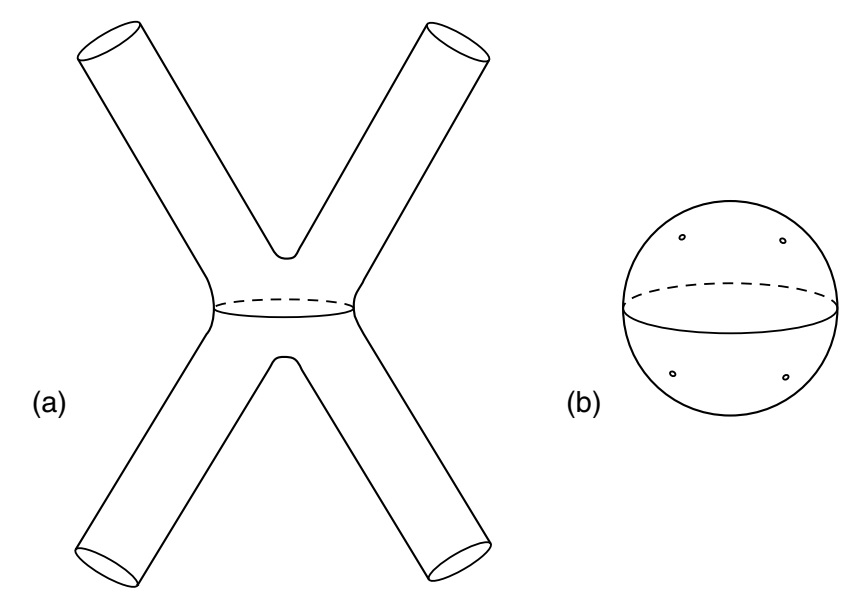
\includegraphics[width=0.8\textwidth,natwidth=645,natheight=450]{Fig3.8.jpg}\\
		\caption{(a) 闭弦的散射, 其中弦的源趋于$X^{0}=\pm \infty$. (b) 4-闭弦散射的共形等价图像: 有非常小的洞的球面.}\label{Fig3.8}
	\end{center}
\end{figure}

所以, 我们现在来考察图\ref{Fig3.8}中所示的过程, 其中源被拉向了无穷远处. 我们将讨论应该如何在路径积分中表示这些源. 远离散射过程, 弦自由地传播, 每个出弦与入弦是一个长圆柱, 可以用一个复坐标$w$描述,
\begin{equation}
-2 \pi t \leq \operatorname{Im} w \leq 0, \qquad w \cong w+2 \pi \:. \label{3.5.1}
\end{equation}
圆柱的下端$\operatorname{Im} w=-2 \pi t$, 是源的结尾, 上端插入世界面的其余部分, 并且圆周是周期$\operatorname{Re} w$方向. 对应于散射过程的极限是$t \rightarrow \infty$. 看起来似乎是我们将时空中的长距离与世界面坐标中的长圆柱混淆, 但这将是较为正确的: 稍后我们将看到, 沿着长时空距离的传播精确来源于这样的世界面, 其中圆柱以以上的意义变长.

我们在第\ref{cha:2}章知道, 圆柱有一等价描述: 
\begin{equation}
z=\exp (-\mi w), \quad \exp (-2 \pi t) \leq|z| \leq 1 \:. \label{3.5.2}
\end{equation}
在这个图景中, 长圆柱映射到了单位圆盘, 其中外弦态是处在中心的圆. 在内部度规的几何中, 图\ref{Fig3.8}a所示的过程现在看起来像是\ref{Fig3.8}b. 在$t \rightarrow \infty$的极限下, 小圆收缩成点, 而世界面退化至对于每一外态则插入一个点的球面.

\begin{figure}[h]
	\begin{center}
		%width=0.8\textwidth,bb=0 0 863 602 
		%1px=0.75pt
		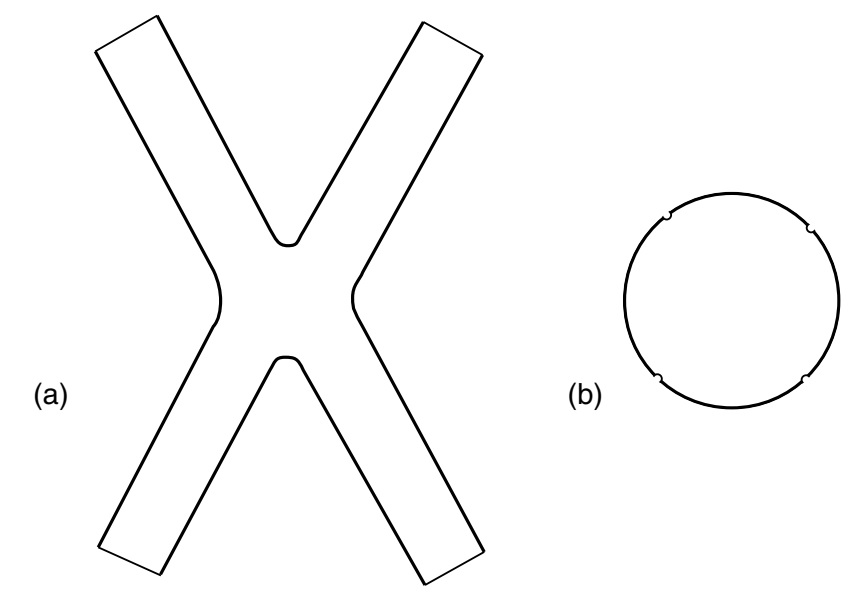
\includegraphics[width=0.8\textwidth,natwidth=645,natheight=450]{Fig3.9.jpg}\\
		\caption{(a) 四个开弦的散射, 其中弦源趋于$X^{0}=\pm \infty$. (b) 共形等价图像: 有凹痕的圆盘.}\label{Fig3.9}
	\end{center}
\end{figure}

同样的概念对外开弦态成立. 图\ref{Fig3.9}a过程中的长带可以描述成
\begin{equation}
-2 \pi t \leq \operatorname{Im} w \leq 0, \quad 0 \leq \operatorname{Re} w \leq \pi \:. \label{3.5.3}
\end{equation}
其中 $\operatorname{Im} w=-2 \pi t$ 是源, 而 $\operatorname{Re} w=0, \pi$ 是端点边界. 在 $z=-\exp (-\mi w)$下, 这映射成单位圆盘与上半平面的交集. 而在原点处切开了一个小的半圆
\begin{equation}
\exp (-2 \pi t) \leq|z| \leq 1, \quad \operatorname{Im} z \geq 0 \:. \label{3.5.4}
\end{equation}
散射过程现在看起来像图\ref{Fig3.9}b. 在$t \rightarrow \infty$的极限下, 源收缩成位于(端点)边界上的点.

这是我们已经看到的态-算符对应. 每个源变成世界面上的一个定域扰动. 对于一个给定的入弦或出弦, 其有$D$-动量$k^{\mu}$以及内部态$j$, 相应地, 存在一个由极限过程决定的定域\emph{顶点算符} $\mathscr{V}_{j}(k)$ . 出态和入态由 $k^{0}$ 符号区分; 对于入态 $k^{\mu}=(E, \mathbf{k})$ 和出态 $k^{\mu}=-(E, \mathbf{k})$, 图\ref{Fig3.8}和\ref{Fig3.9}仅描述了最低阶振幅, 但这个构造是相当普遍的: 我们可以将注意力限制在紧致世界面上, 其上没有一个趋向无限远处的管, 但对于每一外闭弦有一在内部的类点插入. 对于每一外开弦在边界上有一类点插入. 那么一个$n$点$S$-矩阵元为
\begin{align}
&S_{j_{1} \ldots j_{n}}(k_{1}, \ldots, k_{n})  \nonumber \\
&\quad=\sum_{
	\text { compact } \atop \text { topologies}} \frac{[\dif X \, \dif g]}{V_{\text {diff } \times \text { Weyl }}} \exp (-S_{X}-\lambda \chi) 
	\prod_{i=1}^{n} \int \dif^{2} \sigma_{i} \: g(\sigma_{i})^{1 / 2} \mathscr{V}_{j_{i}}(k_{i}, \sigma_{i}) \:. \label{3.5.5}
\end{align}
为了使顶点算符插入diff不变, 我们沿着世界面对它们积分, 在本卷的剩余部分, 将看到我们的猜测是正确的, 并且确定了合理的弦$S$-矩阵. 

依赖于我们所考察的是4种理论的那一个, 对拓扑的求和可能包含非定向世界面和/或带边世界面. 一般而言, 对拓扑的求和不限制在连通世界面; 总的过程可能包含两组或多组独立的粒子散射. 将求和约束在连通世界面上, 进而集中于连通$S$-矩阵是方便的. 

为了获得连通$S$-矩阵, 之后我们必须对世界面所有紧致的、连接的拓扑求和. 在二维中, 拓扑的分类是众所周知的. 任何紧致的、连通的、定向的无边二维平面拓扑上等价于有$g$个柄的球面, $g$称为平面的亏格. 在图\ref{Fig3.10}中, 我们展示了$g=0,1,2$情形.

\begin{figure}[h]
	\begin{center}
		%width=0.8\textwidth,bb=0 0 890 215
		%1px=0.75pt
		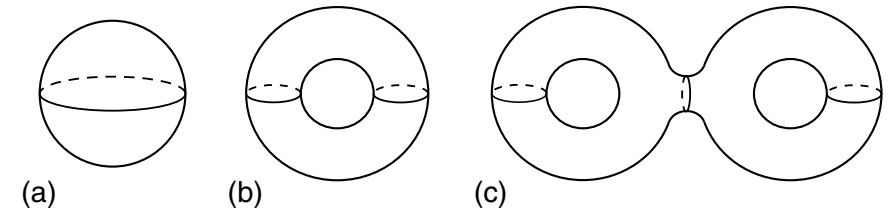
\includegraphics[width=0.8\textwidth,natwidth=667,natheight=161]{Fig3.10.jpg}\\
		\caption{紧致连通定向闭曲面, 其亏格分别为(a) 0, (b) 1, (c) 2.}\label{Fig3.10}
	\end{center}
\end{figure}

通过在闭曲面上剪洞可以增加边界. 任何紧致的, 连通的, 定向二维曲面拓扑等价于有$g$个柄和$b$个洞的球面, 例如$(g,b)=(0,1)$是圆盘, $(0,2)$是圆环, $(0,3)$是裤子. 

为了描述非定向曲面, 引入十字帽是有用的: 在面上剪一个洞并将对径点粘起来. 更细致一些, 取复坐标, 剪出一个略小于单位半径的圆盘, 并将$z^{\prime}=-1 / \bar{z}$ 定义的相反点粘起来. 由于粘合是反全纯的, 所产生的曲面是非定向的. 另外, 不像边界的情况, 十字帽不引入边界或其他定域特征. 由于剪切产生的边界仅是坐标补片的边界, 任何紧致连通闭曲面, 无论定向还是非定向, 总可以在球面上增加$g$个柄和$c$个十字帽获得; 任何紧致连通曲面可通过增加$g$个柄, $b$个边界及$c$个十字帽获得. 实际上, 这些描述有些冗余: 无论是无边还是有边情况, 通过将求和约束至仅令$g$和$c$的一个非零, 就能精确获得. 例如$(g, b, c) = (0, 0, 1)$ 是投影平面, $(g, b, c) = (0, 1, 1)$是Mobius带, $(g, b, c) = (0, 0, 2)$是Klein瓶, 而一个有十字帽的轮胎面可以通过$(g, b, c) = (0, 0, 3)$或$(g, b, c) = (1, 0, 1)$获得, 两个两个十字帽换取一个柄.  Euler数为
\begin{equation}
\chi=2-2 g-b-c \:. \label{3.5.6}
\end{equation}

不同拓扑的数目远小于场论给定阶中不同Feynman图的数目. 例如, 在闭定向理论中, 在微扰论每一阶, 精确存在一个拓扑. 在场论中, 图的数目几何增长. 单个弦图包括所有场论图. 在不同极限下, 柄与它们的圆周相比长得多, 我们可以将柄近似为线, 而弦图在这个极限下近似为对应的Feynman图.


\section{\texorpdfstring{顶点算符}{3.6 Vertex operators}} \label{sec:3.6}

利用态-算符对应, 闭弦快子的顶点算符是
\begin{align}
		V_{0} &=2 g_{\mathrm{c}} \int \dif^{2} \sigma \: g^{1 / 2} \,\me^{\mi k \cdot X}  \nonumber \\
		& \rightarrow g_{\mathrm{c}} \int \dif^{2} z\: : \mathrel{\me^{\mi k \cdot X}}: \:. \label{3.6.1}
\end{align}
我们在映射中引入一个因子$g_{\mathrm{c}}$. 这是闭弦耦合常数, 来自于给过程增加一个额外的弦: 我们将顶点算符的归一化用作耦合的定义. 在第二行, 我们过渡到了平坦世界面. 顶点算符必须是diff且Weyl不变的, 所以, 特别地, 它在平坦世界面上必须是共形不变的. 为了抵消$\dif^2 z$的变换, 算符必须是权重$(1,1)$的张量. 通过一个直接的 OPE 计算, $\me^{\mi k \cdot X}$ 是 权重$h=\tilde{h}=\alpha^{\prime} k^{2} / 4$ 的张量, 所以条件是
\begin{equation}
	m^{2}=-k^{2}=-\frac{4}{\alpha^{\prime}} \:, \label{3.6.2}
\end{equation}
这精确是光锥量子化中所发现的质量.

类似地, 处在第一激发能级的闭弦张量态有平坦世界面顶点算符
\begin{equation}
\frac{2 g_{\mathrm{c}}}{\alpha^{\prime}} \int \dif^{2} z\: : \mathrel{\partial X^{\mu} \bar{\partial} X^{\nu} \me^{\mi k \cdot X}}: \:. \label{3.6.3}
\end{equation}
与快子顶点算符相关的归一化源于态-算符对应, 我们将在第\ref{cha:6}章看到, 相同的相关归一化从$S$-矩阵的归一化中获得. 权重是
\begin{equation}
h=\tilde{h}=1+\frac{\alpha^{\prime} k^{2}}{4} \:, \label{3.6.4}
\end{equation}
所以它们是无质量的, 又一次与光锥量子化相符. 为了使其是一个张量, 存在进一步的条件, 我们将在下面处理.

\subsection*{Polyakov方法中的顶点算符}

在态-算符映射中, 对于任意态, 我们有系统的方法写出平坦世界面顶点算符. 既然世界面总能被变成平坦的, 原则上, 这就是我们需要的全部. 然而现在看来, 研究Polyakov体系中的弯曲世界面顶点算符是有用的. 我们将在本节的剩余部分做这件事. 我们使用的方法将有些笨拙, 并且不像态-算符映射那样系统, 但有些结果是有用的.

任何纳入Polyakov路径积分\eqref{3.5.5}中的算符必须反应理论的定域diff $\times$ Weyl对称性. 我们还没有具体指出\eqref{3.6.1}第一行中的算符是如何在世界面上定义的. 正如之前关于Weyl反常的讨论, 将为方便的方法是保护diff不变性, 并手动检查Weyl变换. 对于大部分用途, 在文献中使用维数正规化. 然而, 对此我们没有大量的需求, 所以将不会引入它; 相反, 我们会推广之前引入的正规编序. 定义重整化算符
\begin{equation}\label{3.6.5}
[\mathscr{F}]_{\mathrm{r}}=\exp \biggl(\frac{1}{2} \int \dif^{2} \sigma \dif^{2} \sigma^{\prime}\: \Delta(\sigma, \sigma^{\prime}) \frac{\delta}{\delta X^{\mu}(\sigma)} \frac{\delta}{\delta X_{\mu}\left(\sigma^{\prime}\right)}\biggr) \mathscr{F} \:.
\end{equation}
这里
\begin{equation}
\Delta(\sigma, \sigma^{\prime})=\frac{\alpha^{\prime}}{2} \ln d^{2}(\sigma, \sigma^{\prime}) \:, \label{3.6.6}
\end{equation}
其中$d(\sigma, \sigma^{\prime})$ 是 $\sigma$ 和 $\sigma^{\prime}$之间的测地距离. 与正规编序相同, \eqref{3.6.5}告诉我们利用 $\Delta(\sigma, \sigma^{\prime})$ 收缩 $\mathscr{F}$中的对, 并对所有可能收缩的方式求和. 在平坦世界面上, $d^{2}(\sigma, \sigma^{\prime})=\lvert z-z^{\prime}\rvert^{2}$并且这退化至共形正规编序. 在弯曲世界面上, 它抵消了 $\mathscr{F}$中的场自收缩产生的奇异积分. Diff不变性是显然的, 但收缩依赖度规, 因此引入了Weyl相关性
\begin{equation}\label{3.6.7}
\delta_{\mathrm{W}}[\mathscr{F}]_{\mathrm{r}}=\left[\delta_{\mathrm{W}} \mathscr{F}\right]_{\mathrm{r}}+\frac{1}{2} \int \dif^{2} \sigma 
\dif^{2} \sigma^{\prime} \:\delta_{\mathrm{W}} \Delta(\sigma, \sigma^{\prime}) \frac{\delta}{\delta X^{\mu}(\sigma)} \frac{\delta}{\delta X_{\mu}(\sigma^{\prime})}[\mathscr{F}]_{\mathrm{r}} \:,
\end{equation}
第一项显现了算符中的Weyl相关性.

动量为$k_\mu$的态, 它的顶点算符在平移下必须按照与态相同的方式变换, 因而形如$\me^{\mi k\cdot X}$与 $X^\mu$ 的导数之积.
在Weyl变换下导数个数不同的算符不会混合, 所以我们从考察零导数开始, 算符\eqref{3.6.1}. Weyl变分来自于显式因子$g^{1/2}$以及\eqref{3.6.7}中给出的重整化
\begin{equation}\label{3.6.8}
\delta_{\mathrm{W}} V_{0}=2 g_{\mathrm{c}} \int \dif^{2} \sigma \: g^{1 / 2}\biggl(2 \delta \omega(\sigma)-\frac{k^{2}}{2} \delta_{\mathrm{W}} \Delta(\sigma, \sigma)\biggr) [\me^{\mi k \cdot X(\sigma)}]_{\mathrm{r}} \:.
\end{equation}
短程时
\begin{equation}
d^{2}(\sigma, \sigma^{\prime}) \approx(\sigma-\sigma^{\prime})^{2} \exp (2 \omega(\sigma)) \label{3.6.9}
\end{equation}
随之
\begin{equation}
\Delta(\sigma, \sigma^{\prime}) \approx \alpha^{\prime} \omega(\sigma)+\frac{\alpha^{\prime}}{2} \ln (\sigma-\sigma^{\prime})^{2} \:. \label{3.6.10}
\end{equation}
在$\sigma^{\prime} \rightarrow \sigma$ 极限下, Weyl变分是非奇异的
\begin{equation}\label{3.6.11}
\delta_{\mathrm{W}} \Delta(\sigma, \sigma)=\alpha^{\prime} \delta \omega(\sigma) \:.
\end{equation}
Weyl变分(\ref{3.6.8})为零的条件就是$k^{2}=4 / \alpha^{\prime}$, 正是前面推导出的结果.


\subsection*{离壳振幅?}

考察一个定义离壳振幅的幼稚尝试: 令$k^\mu$不在质量壳上, 但这与定域世界面对称性不相容. 在位置空间, 这意味着弦世界面的一个定域探测, 在路径积分中插入
\begin{equation}\label{3.6.12}
\delta^{D}(X(\sigma)-x_{0})=\int \frac{\dif^{D} k}{(2 \pi)^{D}} \: \exp [\mi k \cdot(X(\sigma)-x_{0})] \:,
\end{equation}
由于它包含了全部动量所以是不相容的.

从多个角度看, 这并不奇怪. 首先, 前面的讨论, 即我们对弦态可使用点源(顶点算符)要求一个极限过程, 其显著地将我们约束至在壳问题. 
其次, 弦理论包含引力, 而在广义相对论中简单离壳振幅是不存在的. 这是因为我们必须要指定探针的位置, 但坐标是非物理的, 并且坐标不变的离壳量要复杂得多. 第三, 在弦论中我们没有引入额外场以测量定域可观察量的自由度(类似于用以探测强相互作用系统的电弱过程): 我们必须使用弦本身, 或者将我们所讨论的, 理论内蕴的其他客体(D膜和孤子). 

至少在微扰论中是能定义离壳振幅的. 如果固定规范(对此光锥规范是最简单的)并使用弦源. 那么$S$-矩阵公式\eqref{3.5.5}可以用类似于量子场论中的约化公式导出, 先定义有限时间跃迁振幅, 然后再取无限时间极限. 附带地, 读者如若尝试将当前讨论与场论关联起来, 应该注意到路径积分表达\eqref{3.5.5}并不像Green函数, 而更像$S$矩阵元. 场论中类似客体是外传播子被截断的Green函数并且它的外动量被约束在质量壳上.

定域探测\eqref{3.6.12}的讨论也表明了弦之间接触相互作用的问题. 这种相互作用的最简形式将是
\begin{equation}
\int_{M} \dif^{2} \sigma \: g(\sigma)^{1 / 2} \int_{M} \dif^{2} \sigma^{\prime} \: g(\sigma^{\prime})^{1 / 2} \delta^{D}(X(\sigma)-X(\sigma^{\prime}))\:, \label{3.6.13}
\end{equation}
只要世界自交, 这不为零. 然而$\delta$函数包含所有动量, 就像方程\eqref{3.6.12}中那样, 所以这不是Weyl不变的. 弦论的结构相当固定: 弦只能以本章开始所描述的方式与其它弦耦合.

\subsection*{无质量闭弦顶点算符}

尽管有些混乱, 进一步做顶点算符的Polyakov处理是有趣的. 不存在一种方式制造带有一个导数的世界面标量, 所以下一个情况是两个导数. diff不变的可能情况是
\begin{align}
	V_{1}&=\frac{g_{\mathrm{c}}}{\alpha^{\prime}} \int \dif^{2} \sigma \: g^{1 / 2}\Bigl\{ 
		(g^{a b} s_{\mu \nu}+\mi \epsilon^{a b} a_{\mu \nu})
		[\partial_{a} X^{\mu} \partial_{b} X^{\nu} e^{i k \cdot X}]_{\mathrm{r}} \nonumber \\
		&\qquad \qquad \qquad \qquad \qquad \qquad  +\alpha^{\prime} \phi R[\me^{\mi k \cdot X}]_{\mathrm{r}}\Bigr\}  \:, \label{3.6.14}
\end{align}
其中$s_{\mu \nu}, a_{\mu \nu}$,  $\phi$ 分别是对称矩阵, 反对称矩阵和常数. 反对称张量 $\epsilon^{a b}$ 是归一化的,  $g^{1 / 2} \epsilon^{12}=1$或 $g^{1 / 2} \epsilon^{z \bar{z}}=-\mi$. 顶点算符中伴随反对称张量的$\mi$可以理解成Euclidean延拓, 这是因为这一项必有奇数次时间导数(1次). 这一结果广泛应用于Euclidean作用量与顶点算符. 

为了推广Weyl不变性的分析, 我们需要解出高阶的测地距离Weyl相关性(\ref{3.6.11}).
\begin{subequations}\label{3.6.15}
\begin{align}
\partial_{a} \delta_{\mathrm{W}} \Delta(\sigma, \sigma^{\prime})\Bigr\vert_{\sigma^{\prime}=\sigma}&=\frac{1}{2} \alpha^{\prime} \partial_{a} \delta \omega(\sigma) \:, \label{3.6.15a} \\
\partial_{a} \partial_{b}^{\prime} \delta_{\mathrm{W}} \Delta(\sigma, \sigma^{\prime})\Bigr\vert_{\sigma^{\prime}=\sigma}&=\frac{1+\gamma}{2} \alpha^{\prime} \nabla_{a} \partial_{b} \delta \omega(\sigma) \:, \label{3.6.15b} \\
\nabla_{a} \partial_{b} \delta_{\mathrm{W}} \Delta(\sigma, \sigma^{\prime})\Bigr\vert_{\sigma^{\prime}=\sigma}&=-\frac{\gamma}{2} \alpha^{\prime} \nabla_{a} \partial_{b} \delta \omega(\sigma) \:. \label{3.6.15c}
\end{align}
\end{subequations}
这里$\gamma=-\frac{2}{3}$, 为了之后的参考, 我们将其留作参量; 第3个方程可以从第2个方程和第1个方程的梯度得到. 对曲率的变分利用\eqref{3.3.5}, 并对重整化的变分利用\eqref{3.6.7}与\eqref{3.6.15} 
\begin{align}
\delta_{\mathrm{W}} V_{1}&=\frac{g_{\mathrm{c}}}{2} \int \dif^{2} \sigma\: g^{1 / 2} \delta \omega\Bigl\{\left(g^{a b} S_{\mu \nu}+\mi \epsilon^{a b} A_{\mu \nu}\right)[\partial_{a} X^{\mu} \partial_{b} X^{\nu} \me^{\mi k \cdot X}]_{\mathrm{r}}  \nonumber \\
&\qquad \qquad\qquad\qquad \qquad  +\alpha^{\prime} F R[\me^{\mi k \cdot X}]_{\mathrm{r}}\Bigr\} \:, \label{3.6.16}
\end{align}
其中
\begin{subequations}
\begin{align}
S_{\mu \nu}&=-k^{2} s_{\mu \nu}+k_{\nu} k^{\omega} S_{\mu \omega}+k_{\mu} k^{\omega} s_{\nu \omega}-(1+\gamma) k_{\mu} k_{\nu} s^{\omega}{}_{\omega}+4 k_{\mu} k_{\nu} \phi \:,\label{3.6.17a} \\
A_{\mu \nu}&=-k^{2} a_{\mu \nu}+k_{v} k^{\omega} a_{\mu \omega}-k_{\mu} k^{\omega} a_{\nu \omega} \:, \label{3.6.17b} \\
F&=(\gamma-1) k^{2} \phi+\frac{1}{2} \gamma k^{\mu} k^{\nu} s_{\mu \nu}-\frac{1}{4} \gamma(1+\gamma) k^{2} s^{\nu}{}_{\nu}  \:. \label{3.6.17c}
\end{align}
\end{subequations}

在推导Weyl变分(\ref{3.6.16})时, 我们进行了分部积分并使用了关系
\begin{equation}\label{3.6.18}
[\nabla^{2} X^{\mu} \me^{\mi k \cdot X}]_{\mathrm{r}}=\mi \frac{\alpha^{\prime} \gamma}{4} k^{\mu} R\,[\me^{\mi k \cdot X}]_{\mathrm{r}} \:.
\end{equation}
左边本应由于朴素运动方程为零, 但这里运动方程乘上了处在同一点的另一算符. 在该情况下成立的广义原理是算符不需要零, 但它是不独立的——它可以用该理论中其他定域算符展开. 一般而言, 算符的系数依赖于重整化方案; \eqref{3.6.18}可通过取两边的Weyl变分获得.

既然$S_{\mu \nu}, A_{\mu \nu}$ 和 $F$ 所乘为独立算符, Weyl不变的条件是
\begin{equation}
S_{\mu \nu}=A_{\mu \nu}=F=0 \:.\label{3.6.19}
\end{equation}
为了得到算符数目的精确计数, 我们必须注意到不是所有形如(\ref{3.6.14})的$V_1$是独立的. 相反, 在
\begin{subequations}\label{3.6.20}
\begin{align}
s_{\mu \nu} &\rightarrow s_{\mu \nu}+\xi_{\mu} k_{\nu}+k_{\mu} \xi_{\nu} \:, \label{3.6.20a} \\
a_{\mu \nu} &\rightarrow a_{\mu \nu}+\zeta_{\mu} k_{\nu}-k_{\mu} \zeta_{\nu} \:, \label{3.6.20b} \\
\phi &\rightarrow \phi+\frac{\gamma}{2} k \cdot \xi \:, \label{3.6.20c}
\end{align}
\end{subequations}
利用运动方程\eqref{3.6.18}, 可看到$V_1$的变化积分为零. 现在选择满足 $n \cdot k=1$ 和 $n^{2}=0$的矢量$n^{\mu}$. 通过约束
\begin{equation}\label{3.6.21}
n^{\mu} s_{\mu \nu}=n^{\mu} a_{\mu \nu}=0
\end{equation}
就可以获得一组完备的独立算符. 这是$2D$个参量$\xi_{\mu}$ 和 $\zeta_{\mu}$ 的$2D$个方程; 可以证明一个方程和一个参量是平庸的, 但方程组(\ref{3.6.21})中的其他方程是非退化的, 因而定义了一组独立的顶角算符.

通过使用条件(\ref{3.6.21}), 先解出$S_{\mu \nu} n^{\mu} n^{\nu}=0$, 然后解$S_{\mu \nu} n^{\mu}=$ $A_{\mu \nu} n^{\mu}=0$, 最后解$S_{\mu \nu}=A_{\mu \nu}=F=0$, 得到
\begin{subequations}  \label{3.6.22}
\begin{align}
k^{2}&=0 \:, \label{3.6.22a} \\
k^{\nu} s_{\mu \nu}&=k^{\mu} a_{\mu \nu}=0 \:, \label{3.6.22b} \\
\phi&=\frac{1+\gamma}{4} s^{\mu}{}_{\mu} \:. \label{3.6.22c}
\end{align}
\end{subequations}
又一次, 我们发现了质壳条件\eqref{3.6.22a}, 这次对应闭弦的第一激发态. 还有偏振垂直于动量的条件(\ref{3.6.22b}), 这正是无质量张量场的物理偏振所要求的. 在参考系
\begin{equation}
k^{\mu}=(1,1,0,0, \ldots, 0) \: , \quad n^{\mu}=\frac{1}{2}(-1,1,0,0, \ldots, 0) \:, \label{3.6.23}
\end{equation}
条件\eqref{3.6.21}与\eqref{3.6.22b}暗示了所有0分量与1分量为零. 而\eqref{3.6.22c}固定了$\phi$. 这精确留下了$(D-2)^2$个算符, 与光锥规范中所发现的无质量闭弦态数目相同.

移去零模类光偏振需要条件$n^{\mu} s_{\mu \nu}=n^{\mu} a_{\mu \nu}=0$. 然而矢量$n^\mu$的引入明显破坏了Lorentz不变性, 而$n^\mu$的不同选择由于(\ref{3.6.20})等价, 所以理论是Lorentz不变的. 为使理论是Lorentz不变的, 且有一个正的Hilbert空间范数, \eqref{3.6.20}是重要的. 这些关系是定域时空对称性的特征. 特别地, $\xi_{\mu}$是无穷小时空坐标变换, 而$\zeta_{\mu}$是反对称张量场的定域时空对称性. 我们看到了相互作用理论中的定域时空对称性, 而我们在\ref{sec:1.4}节讨论过, 由于无质量自旋1场和自旋2场的存在, 它们必须出现.

我们应该提及一个技术上的问题. 不同的重整化方案赋予重整化算符不同的名字. 最常用的方案是维数正规化; 这一方案中的算符与前面方案的关系为
\begin{subequations} \label{3.6.24}
\begin{align}
[\me^{\mi k \cdot X} ]_{\mathrm{DR}} &= [\me^{\mi k \cdot X}]_{\mathrm{r}} \:, \label{3.6.24a} \\
[\partial_{a} X^{\mu} \me^{\mi k \cdot X}]_{\mathrm{DR}}&=[\partial_{a} X^{\mu} \me^{\mi k \cdot X}]_{\mathrm{r}}  \:, \label{3.6.24b} \\
[\partial_{a} X^{\mu} \partial_{b} X^{\nu} \me^{\mi k \cdot X}]_{\mathrm{DR}}&=[\partial_{a} X^{\mu} \partial_{b} X^{\nu} \me^{\mi k \cdot X}]_{\mathrm{r}}-\frac{\alpha^{\prime}}{12} g_{a b} \eta^{\mu \nu} R\, [\me^{\mi k \cdot X}]_{\mathrm{r}} \:, \label{3.6.24c} \\
[\nabla_{a} \partial_{b} X^{\mu} \me^{\mi k \cdot X}]_{\mathrm{DR}}&=[\nabla_{a} \partial_{b} X^{\mu} e^{i k \cdot X}]_{\mathrm{r}}+ \mi \frac{\alpha^{\prime}}{12} g_{a b} k^{\mu} R\, [\me^{\mi k \cdot X}]_{\mathrm{r}}  \:. \label{3.6.24d}
\end{align}
\end{subequations}
与(\ref{3.6.18})比, 我们看到在维数正规化中$\gamma=0$, 所以运动方程在正规化算符内成立. 这是一个便利, 很多方程简化了. 特别地, 在时空规范变化(\ref{3.6.20})中, $\phi$是不变的.\\

\subsection*{开弦顶点算符}

扩展至开弦是直接的, 仅给出一些结果. 快子顶点算符是
\begin{equation}
g_{\mathrm{o}} \int_{\partial M} \dif s\: [\me^{\mi k \cdot X}]_{\mathrm{r}} \label{3.6.25}
\end{equation}
且对于$k^{2}=1 / \alpha^{\prime}$ 是Weyl不变的. 光子顶点算符是
\begin{equation}
-\mi \frac{g_{\mathrm{o}}}{(2 \alpha^{\prime})^{1 / 2}} e_{\mu} \int_{\partial M} \dif s\: [\dot{X}^{\mu} \me^{\mi k \cdot X}]_{\mathrm{r}} \:, \label{3.6.26}
\end{equation}
其中与快子相关的归一化通过态-算符映射或幺正性获得, $\mi$的出现与闭弦情况相同, 符号是为了方便. 如果 $k^{2}=0$ 且 $k \cdot e=0 $, 这个算符是Weyl不变的. 存在等价关系$e_{\mu} \cong e_{\mu}+\lambda k_{\mu}$, 这是时空规范变换. 这留下了$D-2$个横向偏振. 


\section{\texorpdfstring{弯曲时空中的弦}{3.7 Strings in curved spacetime}} \label{sec:3.7}


现在我们来考察一个重要的新课题: 在弯曲时空中运动的弦. 我们先来回忆下点粒子情况, 它有一个到弯曲时空的自然扩张. 将平坦度规$\eta_{\mu\nu}$替换成一般度规$G_{\mu\nu}$给出作用量
\begin{equation}
S_{\mathrm{pp}}=\frac{1}{2} \int \dif \tau\: \Bigl(\eta^{-1} G_{\mu \nu}(X) \dot{X}^{\mu} \dot{X}^{\nu}-\eta m^{2}\Bigr) \:. \label{3.7.1}
\end{equation}
消掉$\eta$之后, 这变成了沿着粒子世界线的不变固有时. 众所周知, 它的变分给出测地线方程, 代表了粒子在引力场中的运动. 

在Polyakov作用量中作一个相同的替换给出
\begin{equation}
S_{\sigma}=\frac{1}{4 \pi \alpha^{\prime}} \int_{M} \dif^{2} \sigma \:g^{1 / 2} g^{a b} G_{\mu \nu}(X) \partial_{a} X^{\mu} \partial_{b} X^{\nu} \:. \label{3.7.2}
\end{equation}
这是一个自然的猜测, 但读者可能会提出如下异议. 我们已经了解到了引力子本身就是弦的一个态. 一个弯曲时空, 粗略地讲, 是引力子的相干背景, 因而在弦论中它是弦的一个相干态. 仅在作用量\eqref{3.7.2}中放入弯曲度规看起来似乎不足够弦化. 为了看到为什么它是合理的, 考察一个接近平坦的时空
\begin{equation}
G_{\mu \nu}(X)=\eta_{\mu \nu}+\chi_{\mu \nu}(X) \label{3.7.3}
\end{equation}
其中$\chi_{\mu\nu}$很小. 世界面路径积分中的被积函数是                                        
\begin{equation}
\exp(-S_{\sigma})=\exp(-S_{\mathrm{P}})\biggl(1-\frac{1}{4\pi\alpha'}\int \dif^{2}\sigma\:g^{1/2}g^{ab}\chi_{\mu\nu}(X)\partial_{a}X^{\mu}\partial_{b}X^{\nu}+\cdots \biggr) \:. \label{3.7.4}
\end{equation}
$\chi$阶项精确是弦引力子态的顶角算符, 即\eqref{3.6.14}中取
\begin{equation}
\chi_{\mu \nu}(X)=-4 \pi g_{\mathrm{c}} \me^{\mi k \cdot X} s_{\mu \nu}\:. \label{3.7.5}
\end{equation}
所以诚然, 插入弯曲时空确实与我们已知的发生了联系. 作用量(\ref{3.7.2})可视为通过指数化引力子顶点算符来描述引力子的相干态.

这提供了一个自然推广: 将其他无质量弦态的背景也纳入进来. 从顶点算符的形式\eqref{3.6.14}, 有
\begin{equation}\label{3.7.6}
S_{\sigma}=\frac{1}{4 \pi \alpha^{\prime}} \int_{M} \dif^{2} \sigma \: g^{1 / 2}\Bigl[\Bigl(g^{a b} G_{\mu \nu}(X)+ \mi \epsilon^{a b} B_{\mu \nu}(X)\Bigr) \partial_{a} X^{\mu} \partial_{b} X^{\nu}+\alpha^{\prime} R \Phi(X)\Bigr] \:.
\end{equation}
场$B_{\mu\nu}(x)$是反对称张量, 正如运动方程(\ref{3.6.22c})所暗示的, 伸缩子包含$\Phi$与$G_{\mu\nu}$的对角部分. 

作为一个检验, 我们来看看时空规范不变性. 若路径积分的变量变换对应于一个场重定义$X^{\prime \mu}(X)$, 且$G_{\mu \nu}$与$B_{\mu \nu}$按照张量变换, $\Phi$按照标量变换, 
\eqref{3.7.6}是不变的. 从时空观点看, 这是一个坐标变换. 这个作用量同样在
\begin{equation}
\delta B_{\mu \nu}(X)=\partial_{\mu} \zeta_{\nu}(X)-\partial_{\nu} \zeta_{\mu}(X)  \label{3.7.7}
\end{equation}
下不变, 这给Lagrangian密度增加了一个全导数. 这是电磁规范变换到有两个反对称指标的势的推广. 三指标场强
\begin{equation}
H_{\omega \mu \nu}=\partial_{\omega} B_{\mu \nu}+\partial_{\mu} B_{\nu \omega}+\partial_{\nu} B_{\omega \mu} \label{3.7.8}
\end{equation}
是不变的. 存在一个类似的到$n$阶反对称张量势的推广, 其在超弦中扮演了重要角色.

这个理论因此只依赖于度规和其他场所构建的规范不变量. 可以认为场$X^\mu$是流形上的坐标. 这称为靶空间, 因而$X^\mu$定义了一个嵌入
\begin{equation}
\text { 世界面 } \rightarrow \text { 靶 } \:. \label{3.7.9}
\end{equation}
在弦理论中, 靶空间是时空本身. 诸如(\ref{3.7.2})的场论, 其中动能项是场相关的, 因而场空间实际上是弯曲流形, 由于历史原因而被称为非线性$\sigma$模型. 
这个模型在粒子物理与量子场论中有很多应用. 例如, 中性以及带电$\pi$介子场可很好地近似为群流形$SU(2)上$的坐标. 

非线性 $\sigma$模型不再是$X^\mu$的二次型, 所以路径积分现在是一个相互作用二维量子场论. 将路径积分在经典解$X^{\mu}(\sigma)=x_{0}^{\mu}$ 附近展开, 即$X^{\mu}(\sigma)=x_{0}^{\mu}+Y^{\mu}(\sigma)$,
\begin{align}
G_{\mu \nu}(X) \partial_{a} X^{\mu} \partial_{b} X^{\nu} &=\Bigl[G_{\mu \nu}(x_{0})+G_{\mu \nu, \omega}\left(x_{0}\right) Y^{\omega}\nonumber \\
&\quad +\tfrac{1}{2} G_{\mu \nu, \omega \rho}(x_{0}) Y^{\omega} Y^{\rho}+\cdots\Bigr] \partial_{a} Y^{\mu} \partial_{b} Y^{\nu} \:. \label{3.7.10}
\end{align}
展开中第一项是场$Y^\mu$的2次动能项. 接下来一项是立方相互作用, 依次类推. 展开中的耦合常数, $G_{\mu \nu, \omega}(x_{0})$
等, 包含了 $x_{0}$处的导数. 在曲率的特征半径为$R_{\mathrm{c}}$的靶空间中, 度规的导数是$R_{\mathrm{c}}^{-1}$阶的. 因而, 该理论中有效无量纲耦合是 $\alpha'^{1 / 2} R_{\mathrm{c}}^{-1}$. 如果曲率半径 $R_{\mathrm{c}}$ 远大于弦的特征长度, 那么这个耦合是弱的, 并且二维场论的微扰论是个有用的工具. 注意到在同一区域下我们也可采用其他工具. 由于特征长度远大于弦, 我们可以忽略弦的内部结构并使用\emph{低能有效场论}. 正如我们所要看到的, 在决定场论的低能有效作用量时, 弦论进入了. 当约束我们的注意力至无质量背景时, 
我们暗含使用$\alpha^{\prime 1 / 2} R_{\mathrm{c}}^{-1} \ll 1$: 当波长大于弦尺度时, 不产生有质量弦态.

非线性$\sigma$模型\eqref{3.7.2}是可重整理论: 场$Y^\mu$的量纲是0, 因而相互作用的量纲都是2. 然而耦合, 即度规展开式的系数, 在数值上是无限大(除非某些对称性限制了度规的形式). 实际上将度规函数本身, 而非它的展开系数, 定义成交成理论的耦合更有用些.

\subsection*{Weyl不变性}

我们已经强调了Weyl不变性对弦论的相容性是重要的. 仅当二维量子场论是Weyl不变的, 作用量\eqref{3.7.6}将定义一个自洽的弦论. 这个作用量碰巧是在刚性Weyl变换下经典不变的最普遍作用量, 其中在刚性Weyl变换中, $\delta \omega$独立于$\sigma$. 这很容易看到: 在一个刚性Weyl变换下, 有$n$个导数的收缩将正比于$2-n$. 当然, 考察定域Weyl变换也有必要, 在这个变换下, 作用量\eqref{3.7.6}中的 $G_{\mu \nu}$ 和 $B_{\mu \nu}$ 是不变的, 但 $\Phi$ 项不是, 并且包含了对Weyl变换的量子贡献. 在$B_{\mu \nu}$ 和 $\Phi$ 很小,  $G_{\mu \nu}$ 接近$\eta_{\mu \nu}$的极限下, 我们可以使用上述结果寻找Weyl变换. 写下$S_{\sigma}=S_{\mathrm{P}}-V_{1}+\cdots$, 其中$S_{\mathrm{P}}$是平坦空间作用量, 
$V_{1}$是顶点算符\eqref{3.6.14}. 那么
\begin{subequations} \label{3.7.11}
\begin{align}
G_{\mu \nu}(X)&=\eta_{\mu \nu}-4 \pi g_{\mathrm{c}} s_{\mu \nu} \me^{\mi k \cdot X} \:, \label{3.7.11a} \\
B_{\mu \nu}(X)&=-4 \pi g_{\mathrm{c}} a_{\mu \nu} \me^{\mi k \cdot X} \:, \label{3.7.11b} \\
\Phi(X)&=-4 \pi g_{\mathrm{c}} \phi \me^{\mi k \cdot X} \:. \label{3.7.11c}
\end{align}
\end{subequations}
我们当然可以取动量不同的顶点算符的线性组合. 那么, 到首阶, \eqref{3.6.16}给出了Weyl变换; 方便起见, 我们取$\gamma=0$的重整化方案. 
像\eqref{3.4.6}中那样将Weyl变换与$T^{a}{}_{a}$关联起来给出
\begin{equation}
T^{a}{}_{a}=-\frac{1}{2 \alpha^{\prime}} \beta_{\mu \nu}^{G} g^{a b} \partial_{a} X^{\mu} \partial_{b} X^{\nu}-\frac{i}{2 \alpha^{\prime}} \beta_{\mu \nu}^{B} \epsilon^{a b} \partial_{a} X^{\mu} \partial_{b} X^{\nu}-\frac{1}{2} \beta^{\Phi} R
\end{equation}
其中, 到$\chi_{\mu \nu}, B_{\mu \nu}$和$\Phi$ 的线性阶,
\begin{subequations}\label{3.7.13}
\begin{align}
\beta_{\mu \nu}^{G} &\approx-\frac{\alpha^{\prime}}{2}\Bigl(\partial^{2} \chi_{\mu \nu}-\partial_{\nu} \partial^{\omega} \chi_{\mu \omega}-\partial_{\mu} \partial^{\omega} \chi_{\omega \nu}+\partial_{\mu} \partial_{\nu} \chi^{\omega}{}_{\omega}\Bigr)+2 \alpha^{\prime} \partial_{\mu} \partial_{\nu} \Phi \:,  \label{3.7.13a}\\
\beta_{\mu \nu}^{B} &\approx-\frac{\alpha^{\prime}}{2} \partial^{\omega} H_{\omega \mu \nu} \:, \label{3.7.13b}\\
\beta^{\Phi} & \approx \frac{D-26}{6}-\frac{\alpha^{\prime}}{2} \partial^{2} \Phi \:. \label{3.7.13c}
\end{align}
\end{subequations}
在$\beta^{\Phi}$中,  我们引入了\ref{sec:3.4}节所发现的平坦时空反常, 其中暗含了来自于鬼场的正比于26的贡献. 用$\beta$表示$T^{a}{ }_{a}$中的系数是因为它们显然是重整化群$\beta$-函数, 控制了物理对世界面尺度的依赖. 我们将进一步讨论这个.

Weyl反常\eqref{3.7.13}有来自高阶场的进一步贡献. 例如, 将路径积分展开至\eqref{3.7.10}中的三次项的二阶, 那么两个相互作用彼此接近会产生发散. 
它们的OPE包含形如 $|z|^{-2} \partial X^{\mu} \bar{\partial} X^{\nu}$ 乘以 $G_{\alpha \beta} $ 导数的平方的奇异性.  Diff不变要求这个积分以不变距离的形式, $|z| \exp (\omega)>a_{0} $被截断. 这引入了对度规尺度的依赖性, $\ln z_{\min }=-\omega+\ln a_{0}$. Weyl 变分 $\beta_{\mu \nu}^{G}$
因而得到了正比于 $O(G_{\alpha \beta, \gamma})^{2}$ 的贡献, 这个贡献组合线性二阶导数项以构成时空里奇张量.

我们再次不讨论细节, 但引用保留所有项直至两个导数的结果
\begin{subequations}\label{3.7.14}
\begin{align}
\beta_{\mu \nu}^{G}&=\alpha^{\prime} \bm{R}_{\mu \nu}+2 \alpha^{\prime} \nabla_{\mu} \nabla_{\nu} \Phi-\frac{\alpha^{\prime}}{4} H_{\mu \lambda \omega} H_{\nu}{}^{\lambda \omega}+O(\alpha^{\prime 2}) \:, \label{3.7.14a} \\
\beta_{\mu \nu}^{B}&=-\frac{\alpha^{\prime}}{2} \nabla^{\omega} H_{\omega \mu \nu}+\alpha^{\prime} \nabla^{\omega} \Phi H_{\omega \mu \nu}+O(\alpha^{\prime 2}) \:, \label{3.7.14b} \\
\beta^{\Phi}&=\frac{D-26}{6}-\frac{\alpha^{\prime}}{2} \nabla^{2} \Phi+\alpha^{\prime} \nabla_{\omega} \Phi \nabla^{\omega} \Phi-\frac{\alpha^{\prime}}{24} H_{\mu \nu \lambda} H^{\mu \nu \lambda}+O(\alpha^{\prime 2}) \:. \label{3.7.14c} 
\end{align}
\end{subequations}
\eqref{3.7.14}中的几项可以从线性近似\eqref{3.7.13}中辨认出来, 但现在在时空坐标的变换下变得协变. 为了与世界面里奇张量$R_{a b} $区分, 
时空里奇张量是$\bm{R}_{\mu \nu}$. 有更多导数的项是世界面$\alpha^{1 / 2} R_{\mathrm{c}}^{-1}$展开中的高阶项. 
进行高阶Weyl反常计算的最有效方法不是我们所描述的, 而是维数正规化. 

世界面是Weyl不变的, 因而条件是
\begin{equation}
\beta_{\mu \nu}^{G}=\beta_{\mu \nu}^{B}=\beta^{\Phi}=0 \:. \label{3.7.15}
\end{equation}
它们看起来是合理的运动方程. 方程$\beta_{\mu \nu}^{G}=0$类似于有反对称张量场和伸缩子场作为源项的Einstein方程. $\beta_{\mu \nu}^{B}=0$是Maxwell方程的反对称张量推广, 
决定了场强的发散.

\subsection*{背景}
场方程的另一定性特征现在能够理解了: 场$\Phi$总是带着微分出现的, 所以它在$X$无关偏移下不变. 这是因为这样的偏移对作用量\eqref{3.7.6}造成的改变正比于Euler数, 
因而并不影响类似Weyl不变的定域性质. 特别地, 背景
\begin{equation}
G_{\mu \nu}(X)=\eta_{\mu \nu}, \quad B_{\mu \nu}(X)=0, \quad \Phi(X)=\Phi_{0}
\end{equation}
对于任何常数$\Phi_0$是Weyl不变的. 这正是平坦时空作用量\eqref{3.2.2}, 其中
\begin{equation}
\lambda=\Phi_{0} \:. \label{3.7.17}
\end{equation}
$\lambda$的值决定弦之间的耦合强度, 但我们现在看到这个参量的不同值并不意味着存在不同的弦理论.  $\lambda$不同值并不对应不同的理论, 而是对应同一理论中的不同\emph{背景}. 
出现在Nambu-Goto和Polyakov作用量中的其他参量, Regge斜率$\alpha^{\prime}$, 也不是真的自由参量, 因为它是有量纲的. 它定义了长度单位, 可以被吸收进$X^{\mu}$的定义中. 

以二维的观点看, 改变世界面作用量中的场$G_{\mu \nu}, B_{\mu \nu}$和$\Phi$似乎会给出一个新的理论. 从纯弦论的观点看, 这仅是在同一理论下观察不同的背景——一个不同的态. 
这是弦论吸引人的特征之一. 在标准模型中, 以及大多数在量子场论框架下统一标准模型的尝试中, 存在很多不由理论决定的常数; 这些常数的任何值给出一个相容的理论. 在弦论中, 不存在这样的自由参量——耦合常数依赖于态且原则上由动力学决定. 当然, 目前来看, 这仅是把困难移到了别处, 因为我们对动力学的理解程度不足以知道背景场的值.

令人惊讶的是, Einstein方程在一个看起来不同寻常的地方出现了, 它作为二维场论Weyl不变的条件. 弦论提供了这两个概念的联系. 同样引人注意的是, 仅在满足合适场方程的背景中, 弦的传播才是自洽的. 这类似于我们早期的发现: 只有在壳顶点算符是有意义的.

另一发现: 条件 $D=26$来自$T^{a}{}_{a}$中的$R$项. 在非线性$\sigma$模型中, 这被推广至$\beta^{\Phi}=0$. 
我们在\eqref{3.7.14c}中看到 $\beta^{\Phi}$中的领头阶正比于$D-26$, 但存在包含场梯度的修正. 显然, 如果场不是常数, 我们有另一$D$值. 这是正确的, 
尽管我们不能真的从\eqref{3.7.14c}中得到它, 因为这是在近似 $\alpha^{\prime 1 / 2} R_{\mathrm{c}}^{-1} \ll 1$ 下导出的, 而其中 $\beta^{\Phi}$ 的修正很小. 事实上,  $D \neq 26$ 的精确解是知道的. 我们现在给出一个例子: 
\begin{equation}\label{3.7.18}
G_{\mu \nu}(X)=\eta_{\mu \nu}, \quad B_{\mu \nu}(X)=0, \quad \Phi(X)=V_{\mu} X^{\mu} \:.
\end{equation}
如果
\begin{equation}
V_{\mu} V^{\mu}=\frac{26-D}{6 \alpha^{\prime}} \:, \label{3.7.19}
\end{equation}
$\beta$-函数(\ref{3.7.14})为零. 这个结果实际上是\emph{精确}的, 因为场\eqref{3.7.18}关于$X^\mu$是常数或线性的, 所以世界面路径积分仍然是高斯型. 
对$g_{a b}$变分来决定这个理论的$T_{a b}$ , 发现它正是伸缩子CFT, 中心荷$c=D+6 \alpha^{\prime} V_{\mu} V^{\mu}$在条件\eqref{3.7.19}下确定是26. 
由于$\Phi$必须有一个大的梯度以改变$D$, 这个CFT并不描述我们近似平坦且齐次的4维时空, 但它可能有宇宙学上的应用. 这个CFT同样是重要的, 
因为$D=1$和$D=2$的情况对弦论是足够简单以至于精确可解的.

\subsection*{时空作用量}

场方程\eqref{3.7.15}可从时空作用量
	\begin{align}
		\bm{S}&=\frac{1}{2 \kappa_{0}^{2}} \int \dif^{D} x\: (-G)^{1 / 2} \me^{-2 \Phi} \biggl[- \frac{2(D-26)}{3 \alpha^{\prime}}+\bm{R}-\frac{1}{12} H_{\mu \nu \lambda} H^{\mu \nu \lambda}  \nonumber \\
		&\qquad\qquad\qquad\qquad \qquad\qquad+4 \partial_{\mu} \Phi \partial^{\mu} \Phi+O(\alpha^{\prime})\biggr]  \label{3.7.20}
	\end{align}
导出. 归一化常数$\kappa_0$不由场方程决定, 并且由于它可以通过$\Phi$的重定义被改变, 所以在物理上不是很重要. 可以证明
\begin{align}
\delta \bm{S}&=-\frac{1}{2 \kappa_{0}^{2} \alpha^{\prime}} \int \dif^{D} x\: (-G)^{1 / 2} \me^{-2 \Phi} \Bigl[\delta G_{\mu \nu} \beta^{G \mu \nu}+\delta B_{\mu \nu} \beta^{B \mu \nu} \nonumber \\
&\qquad \qquad +\Bigl(2 \delta \Phi-\tfrac{1}{2} G^{\mu \nu} \delta G_{\mu \nu}\Bigr) (\beta^{G \omega}{}_{\omega}-4 \beta^{\Phi})\Bigr] \:. \label{3.7.21}
\end{align}
作用量用$\bm{S}$表示是表明它是控制低能时空场的有效作用量. 

做如下形式的场重定义 
\begin{equation}
\tilde{G}_{\mu \nu}(x)=\exp (2 \omega(x)) G_{\mu \nu}(x) \:, \label{3.7.22}
\end{equation}
这是时空Weyl变换. 由$\tilde{G}_{\mu \nu}$构造的里奇标量是
\begin{equation}
\tilde{\bm{R}}=\exp (-2 \omega)\Bigl[\bm{R}-2(D-1) \nabla^{2} \omega-(D-2)(D-1) \partial_{\mu} \omega \partial^{\mu} \omega\Bigr] \:. \label{3.7.23}
\end{equation}
对于特殊情况$D=2$, 这是Weyl变换\eqref{3.3.5}. 令$\omega=2(\Phi_{0}-\Phi) /(D-2)$, 并定义
\begin{equation}
\tilde{\Phi}=\Phi-\Phi_{0} \:, \label{3.7.24}
\end{equation}
其有一个归零的期望值. 作用量变成
\begin{align}
\bm{S} &= \frac{1}{2 \kappa^{2}} \int \dif^{D} X\: (-\tilde{G})^{1 / 2}\biggl[-\frac{2(D-26)}{3 \alpha^{\prime}} \me^{4 \tilde{\Phi} /(D-2)}+\tilde{\bm{R}} \nonumber \\
&\quad -\frac{1}{12} \me^{-8 \tilde{\Phi} /(D-2)} H_{\mu \nu \lambda} \tilde{H}^{\mu \nu \lambda}-\frac{4}{D-2} \partial_{\mu} \tilde{\Phi} \tilde{\partial}^{\mu} \tilde{\Phi}+O(\alpha^{\prime})\biggr] \:, \label{3.7.25}
\end{align}
其中波浪号是作为一个提醒: 指标是通过$\tilde{G}^{\mu \nu}$升降的. 以$\tilde{G}_{\mu \nu}$的形式, 引力拉格朗日密度取标准形式$(-\tilde{G})^{1 / 2} \tilde{\bm{R}} / 2 \kappa^{2}$. 常数$\kappa=\kappa_{0} \me^{\Phi_{0}}$ 是观察到的引力耦合常数,
\begin{equation}
\kappa= (8 \pi G_{\mathrm{N}})^{1 / 2}=\frac{(8 \pi)^{1 / 2}}{M_{\mathrm{P}}}=(2.43 \times 10^{18} \:\mathrm{GeV})^{-1} \:. \label{3.7.26}
\end{equation}
普遍地,  $G_{\mu \nu}$被称为$\sigma$模型度规或弦度规, 而$\tilde{G}_{\mu \nu}$称为Einstein度规. 由于有交换伸缩子的力, 不存在等效原理, 因而没办法挑出度规的一个优先定义. 更进一步, 在弦论中存在可以赋予伸缩子质量以及一个有限范围的高阶效应——这是好事, 因为等效原理确实以非常高的精度成立.


注意到伸缩子总出现在作用量\eqref{3.7.20}的总因子$\me^{-2 \Phi}$中, 并且在其他地方总是以微分形式出现. 这与如下事实是一致的: 给伸缩子增加一个总常数对Weyl反常没有影响. 从时空的观点看, 这给作用量乘上了一个常数, 但不影响运动方程. 它也反应了这样的事实: 在量子场论中, 总可以调节场使得耦合常数$g$作为一个总因子$g^{-2}$出现, 
且在弦论中则是$\me^{-2 \Phi}$. 例如, Yang-Mills作用量通常以如下形式引入
\begin{subequations} \label{3.7.27}
\begin{align}
\bm{S} &=-\frac{1}{4} \int \dif^{D} x \: \operatorname{Tr}(F_{\mu \nu} F^{\mu \nu}) \:, \label{3.7.27a} \\
F_{\mu \nu}&=\partial_{\mu} A_{\nu}-\partial_{\nu} A_{\mu}-\mi g[A_{\mu}, A_{\nu}] \:. \label{3.7.27b}
\end{align}
\end{subequations}
通过定义
\begin{equation}
g A_{\mu}=A_{\mu}^{\prime}\:, \qquad g F_{\mu\nu}=F_{\mu\nu}^{\prime} \:, \label{3.7.28}
\end{equation}
$g$从场强, 协变导数以及规范变换中被消除了, 而以一个总因子$g^{-2}$出现在作用量中. 在弦论中, 当作用量用世界面上的场表示时, 这是成立的. 
如果我们做一个与伸缩子相关的重定义, 就像推导\eqref{3.7.25}所要做的, 那么这不再成立.

当$g$仅在作用量的归一化中出现时, 每个传播子包含一个$g^{2}$因子, 每个相互作用包含$g^{-2}$. 不难证明对有效作用量的$L$-圈贡献中传播子比顶点多 $L{-}1$个, 
所以它的标度是$g^{2(L-1)}$. 在弦论中, 这是$\me^{-\chi \Phi}$, 也是我们所期待的.

背景的讨论可扩至开弦. 我们已经看到开弦顶点算符是沿着边界积分的, 所以开弦场作为边界项出现在$\sigma$模型作用量中.


\subsection*{紧致化与 CFT}
目前为止研究的四种弦论(有没有边界, 定向或非定向)有一些共同的特征: 一个很好的特征是会自动包含广义相对论, 也存在几个坏特征: 需要26维, 存在快子, 以及频谱中没有费米子. 然而, 广义相对论的出现为额外维给出了一种自然解释. 在广义相对论中, 时空的几何是动力学的, 不是固定的. 平坦时空仅是场方程众多解中的一个. 可能存在一些解, 其中有些维很大且平坦, 而其他的很小且高度蜷曲. 度规是
\begin{equation}\label{3.7.29}
g_{M N}=\begin{bmatrix}
\eta_{\mu \nu} & 0 \\
0 & g_{m n}(x^{p})
\end{bmatrix} \:.
\end{equation}
我们已经把26个坐标$M,N=0,\cdots,25$分成四个时空坐标 $\mu, \nu=0, \cdots, 3$ 和 22 个内部坐标 $m, n, p=4, \cdots, 25$. 
度规\eqref{3.7.29}在四维是平坦的, 但在其他22维是蜷曲的. 假定内部空间紧致. 一个例子: 若伸缩子场是一个常数, 那么至$\alpha^{\prime}$阶, 背景场方程\eqref{3.7.15}是满足的, 
反对称张量是零, 内部空间是里奇平坦的, $\bm{R}_{m n}=0$.

换句话说, 时空形式为 $M^{d} \times K$,其中$M^{d}$是$d$维闵可夫斯基空间,  $K$ 是某种 $(26-d)$ 维紧致黎曼空间. 在这样的时空中, 尺度远大于$K$的物理与$d$维闵可夫斯基时空的物理是相同的. 独立于弦论, 有很好的理由考虑时空是这一形式的可能性.

我们可以考虑进一步推广这个概念. 基本的物理相容性条件就那么几个. 我们要求Lorentz不变性, 要求量子力学几率为正且守恒——迄今为止, 弦论中似乎没有什么要求标准量子力学的基础被修正, 尽管对其有不同认识将是有趣的. 尽管这些条件是简单的, 但它们在规范理论, 引力和弦论之间存在一些冲突. 在显然协变规范中存在着必须从物理振幅中退耦负范类时激发. 在光锥规范中, 内积是正定的

因此一个必要条件是二维diff不变性, 使得非物理振子仅是坐标系统的振子. Weyl不变性是一个更加技巧的要求: 丢失Weyl不变性所产生的额外自由度没有坐标系统振子那么直观.

我们也将做一个额外的技巧性假定:  出现在世界面作用量中的嵌入时$X_0$仅在
\begin{equation}\label{3.7.30}
-\frac{1}{4 \pi \alpha^{\prime}} \int_{M} \dif^{2} \sigma \: g^{1 / 2} g^{a b} \partial_{a} X^{0} \partial_{b} X^{0} \:.
\end{equation}
例如, 在$\sigma$模型中, 这意味着场是静态的,  $G_{0 \mu}=\eta_{0 \mu}$ 且 $B_{0 \mu}=0 $. 这一假定算不上一个约束. 如果感兴趣的是静态,  \eqref{3.7.30}就足够了. 
时间相关的背景也肯定是重要的, 但除了在时间尺度就是弦尺度的极端情况下, 它们可以用低能有效场论来分析. 做出假定\eqref{3.7.30}的原因是要把主要问题, $X^0$的错号特征, 放在一个明显的形式中. 

要求体现定域不变性导致了对更加普遍弦论的如下提议: 将25个空间场$X^{\mu}$替换成任何有$c=\tilde{c}=25$的幺正CFT. 这确保了整个二维理论, 包含$X^{0}$和鬼, 可以以一种(diff $\times$ Weyl)不变的方式与弯曲度规耦合. 幺正(正定内积)条件是必须的, 因为仅存在足够的定域规范对称性以移除非物理$X^{0}$激发; 世界面内积在这里是相关的, 因为它在单粒子分区变成了时空内积. 在第二卷, 我们将看到进一步的推广是可能的, 同时扩大了定域对称群与非物理激发的集合.                                            

如果我们感兴趣的是低能物理看起来像四维的, 我们保持自由场$X^{\mu}$,  $\mu=0,1,2,3$, 而将剩余的$X^{\mu}$ 替换成 $c=\tilde{c}=22$的紧致幺正CFT. 
对于紧致化, 我们意指频谱是离散的, 就像有限体积内的量子场论. 存在一些构建所有的CFT尝试, 我们将在15章描述. 
所有这些理论都有快子, 内部CFT中的幺正态 $|1\rangle$ 与四维CFT基态 $|0 ; k\rangle$的乘积.

我们所作的推广有多大?如果定域对称性是唯一显著的约束, 我们可以在世界面上随意引入有不同的世界面和时空量子数的场. 这似乎使得我们远离了原始的26个$X^\mu$场. 然而在二维中, 在看似不同的量子场论之间存在很多等价性, 使得情况不那么显然.

一般而言, 基于不同CFT但有相同的世界面对称性以及拓扑的所有弦论是统一理论的不同基态. 这引起了语义上的问题: 尽管世界面拉格朗日量不同的弦论可能只是同一理论的不同真空,  但我们通常称它们为不同的理论.
\setcounter{section}{0}%更改chapter的计数器值
%\numberwithin{equation}{chapter}%公式计数器从属于节计数器
\numberwithin{equation}{section}%公式计数器从属于节计数器
\numberwithin{figure}{section}%图计数器从属于节计数器
\setcounter{chapter}{3}

%\chapter{\texorpdfstring{弦谱}{4 The string spectrum}}
\chapter{弦谱}
%\section{\texorpdfstring{旧的协变量子化}{4.1 Old covariant quantization}}
\section{旧的协变量子化}
在共形规范下,世界面场是 $X^{\mu}$ 以及Faddeev-Popov 鬼场 $b_{a b}$ 与 $c^{a} $. Hilbert比实际的弦的物理频谱要大:  D 组 $\alpha^{\mu}$ 振子包含坐标系的非物理振荡,并且存在鬼振子. 这普遍是协变规范中的情况,存在来自类时振子(由于对易子正比于时空度规 $\eta_{\mu v}$)的负范态,以及来自鬼场的负范态.\\
实际的物理空间更小. 为了看到如何辨认这个更小的空间,考察某个初态$|i\rangle$ 传播到某个末态 $|f\rangle $的无限圆柱上的振幅.  假定初时我们使用定域对称性以固定度规为形式 $g_{a b}(\sigma) $. 现在考察一个不同的规范,度规为 $g_{a b}(\sigma)+\delta g_{a b}(\sigma)$. 物理振幅应该不依赖于这个选择;当然,对于度规的改变,我们知道路径积分如何变化. 从$T^{a b}$的定义(3.4.4) 
\begin{equation}
\delta\langle f \mid i\rangle=-\frac{1}{4 \pi} \int d^{2} \sigma g(\sigma)^{1 / 2} \delta g_{a b}(\sigma)\left\langle f\left|T^{a b}(\sigma)\right| i\right\rangle
\end{equation}
为了使对于度规的任意改变变分为零,我们需要
\begin{equation}\label{4.1.2}
\left\langle\psi\left|T^{a b}(\sigma)\right| \psi^{\prime}\right\rangle=0
\end{equation}
其中 $|\psi\rangle,\left|\psi^{\prime}\right\rangle$ 是任意的态.\\
考虑它的另一种方式.  从 $g_{a b}$ 的变分得到的原始运动方程是 $T^{a b}=0 $.  在固定规范后,这并不作为一个算符方程成立:由于我们在规范固定理论中没有变化 $g_{a b}$ ,我们缺失了一个方程. 条件 (\ref{4.1.2})称缺失的运动方程,必须对物理态之间的任何矩阵元成立. 当我们变换规范时,必须将Faddeev–Popov行列式的变化考虑在内. 所以矩阵元中的能动量张量是$X^\mu$贡献与鬼场贡献之和:
\begin{equation}
T_{a b}=T_{a b}^{X}+T_{a b}^{\mathrm{g}}
\end{equation}
$X^\mu$可以被更加普遍的CFT替代(我们指代物质CFT). 在这个情况下
\begin{equation}
T_{a b}=T_{a b}^{\mathrm{m}}+T_{a b}^{\mathrm{g}}
\end{equation}
在本节的剩余部分,我们将以一种简单却有些特殊的方式(ad hoc way)强加条件(\ref{4.1.2}),这称为旧协变量子化(OCQ). 对于很多用处,它是足够的. 在下一节,我们将采取一个更加系统的方法,BRST量子化. 它们实际上是等价的,这将在4.4节证明.\\
在这个特殊方法中,我们将简单地忽视鬼场并尝试约束物质Hilbert空间,使得缺失的运动方程$T_{a b}^{\mathrm{m}}=0$ 对于矩阵元成立. 以Laurent系数的形式,这是 $L_{n}^{\mathrm{m}}=0$, 在闭弦中又有 $\tilde{L}_{n}^{\mathrm{m}}=0 $. 可以先尝试要求物理态对于所有的n满足$L_{n}^{m}|\psi\rangle=0$ , 但这太强了;用 $L_{m}^{\mathrm{m}}$作用这个方程,并构成对易子. 由于 Virasoro代数中的中心荷,会遇到不一致. 然而,只要Virasoro下降,且零算符湮灭物理态,就是足够的
\begin{equation}\label{4.1.5}
\left(L_{n}^{\mathrm{m}}+A \delta_{n, 0}\right)|\psi\rangle=0 \quad \text { for } n \geq 0
\end{equation}
那么,对于n<0,我们有
\begin{equation}
\left\langle\psi\left|L_{n}^{\mathrm{m}}\right| \psi^{\prime}\right\rangle=\left\langle L_{-n}^{\mathrm{m}} \psi \mid \psi^{\prime}\right\rangle=0
\end{equation}
我们使用了
\begin{equation}\label{4.1.7}
L_{n}^{\mathrm{m} \dagger}=L_{-n}^{\mathrm{m}}
\end{equation}
这源于能动量张量的Hermiticity. (\ref{4.1.5})与Virasoro代数是一致的. 当n=0,我们像往常一样引入序列常数的可能. 满足(\ref{4.1.5}) 的态是物理的.\\
以(2.9.8)的术语,物理态是权重-A的最高权重态. (\ref{4.1.5})类似量子电动力学的Gupta量子化. 利用共轭伴(\ref{4.1.7}),可看到态的形式为
\begin{equation}\label{4.1.8}
|\chi\rangle=\sum_{n=1}^{\infty} L_{-n}^{\mathrm{m}}\left|\chi_{n}\right\rangle
\end{equation}
它正交于任何 $\left|\chi_{n}\right\rangle $的所有物理态. 这样的态称为伪态(spurious). 一个既是物理的,又是伪的态,称为空(null). 如果 $|\psi\rangle$是物理的, $|\chi\rangle$是空的, 那么 $|\psi\rangle+|\chi\rangle$ 也是物理的,且任何物理态与它的内积和与$|\psi\rangle$的内积相同. 因而这两个态物理上不可分辨. 我们等同
\begin{equation}
|\psi\rangle \cong|\psi\rangle+|\chi\rangle
\end{equation}
那么真实物理态是等价类的集合
\begin{equation}
\mathscr{H}_{\mathrm{OCQ}}=\frac{\mathscr{H}_{\text {phys }}}{\mathscr{H}_{\text {null }}}
\end{equation}
我们来看看,对于平坦时空中的开弦的前两个等级,这是如何运作的,不必假定D=26. 唯一的相关项是
\begin{subequations}
\begin{equation}
L_{0}^{\mathrm{m}}=\alpha^{\prime} p^{2}+\alpha_{-1} \cdot \alpha_{1}+\ldots
\end{equation}
\begin{equation}
L_{\pm 1}^{\mathrm{m}}=\left(2 \alpha^{\prime}\right)^{1 / 2} p \cdot \alpha_{\pm 1}+\ldots
\end{equation}
\end{subequations}

\begin{proof}
对于开弦,由(2.7.25)
$$
\alpha_{0}^{\mu}=\left(2 \alpha^{\prime}\right)^{1 / 2} p^{\mu}
$$
$$
\alpha^{\prime} P^{2}=\frac{\alpha^{\prime}}{2 \alpha^{\prime}} \alpha_{0} \cdot \alpha_{0}=\frac{1}{2} \alpha_{0} \cdot \alpha_{0}
$$
$$
\left(2 \alpha^{\prime}\right)^{1 / 2} p \cdot \alpha_{\pm 1}=\alpha_{0} \cdot \alpha_{\pm 1}
$$
\end{proof}
\noindent
最低质量能级唯一态是 $ | 0 ; k \rangle $.  此能级唯一非平庸条件是 $\left(L_{0}^{\mathrm{m}}+A\right)|\psi\rangle=0$, 
\quad 给出$m^{2}=A / \alpha^{\prime} $.  
这一能级不存在空态.  伪态(\ref{4.1.8}) 中 Virasoro生成元全部包含上升算符,因而存在一个等价类,对应标量粒子.\\


\fbox{\noindent\centering\parbox{0.9\textwidth}{补充:$m^{2}=A / \alpha^{\prime} $的证明\\
	$$
	\left.L_{0}^{m}|\psi\rangle=\alpha^{\prime} p^{2} / \psi\right\rangle=-\alpha^{\prime} m^{2}|\psi\rangle
	$$
	$$
	\therefore \alpha^{\prime} m^{2}=A
	$$}}\\

\noindent
在下一能级,存在D个态
\begin{equation}
|e ; k\rangle=e \cdot \alpha_{-1}|0 ; k\rangle
\end{equation}
范数是
\begin{equation}\label{4.1.13}
\begin{aligned}
\left\langle e ; k \mid e ; k^{\prime}\right\rangle &=\left\langle 0 ; k\left|e^{*} \cdot \alpha_{1} e \cdot \alpha_{-1}\right| 0 ; k^{\prime}\right\rangle \\
&=\left\langle 0 ; k\left|\left(e^{*} \cdot e+e^{*} \cdot \alpha_{-1} e \cdot \alpha_{1}\right)\right| 0 ; k^{\prime}\right\rangle \\
&=e^{\mu *} e_{\mu}(2 \pi)^{D} \delta^{D}\left(k-k^{\prime}\right)
\end{aligned}
\end{equation}
我们使用了
\begin{equation}
\alpha_{n}^{\mu \dagger}=\alpha_{-n}^{\mu}
\end{equation}
其源于$X^\mu$的Hermiticity ,以及
\begin{equation}
\left\langle 0 ; k \mid 0 ; k^{\prime}\right\rangle=(2 \pi)^{D} \delta^{D}\left(k-k^{\prime}\right)
\end{equation}
类时激发有一个负范态.\\
$L_{0}^{\mathrm{m}}$条件给出
\begin{equation}
m^{2}=\frac{1+A}{\alpha^{\prime}}
\end{equation}
\begin{proof}
	$$
	\begin{array}{l}
	L_{0}^{m}\left|e; k\right\rangle=\alpha^{\prime} p^{2}|e ; k\rangle+\alpha_{-1} \cdot \alpha_{1} e \cdot \alpha_{-1}|0 ; k\rangle \\
	\left.=\left|-\alpha^{\prime} m^{2}\right| e; k\right\rangle+\alpha_{-1}^{\mu} e^{\nu}\left(\eta_{\mu \nu}+\alpha_{-1\nu}\alpha_{1, \mu}\right)|0 ; k\rangle \\
	=-\alpha^{\prime} m^{2}\left|e;k\right\rangle+e \cdot \alpha_{-1}\left|0; k\right\rangle \\
	=\left(1-\alpha^{\prime} m^{2}\right)\left|e; k\right\rangle
	\end{array}
	$$
	$$
	\therefore A=\alpha^{\prime} m^{2}-1
	$$
\end{proof}
其他非平庸物理态条件是
\begin{equation}
L_{1}^{\mathrm{m}}|e ; k\rangle \propto p \cdot \alpha_{1} e \cdot \alpha_{-1}|0 ; k\rangle=e \cdot k|0 ; k\rangle=0
\end{equation}
因而$k \cdot e=0$,在这一能级存在伪态
\begin{equation}
L_{-1}^{\mathrm{m}}|0 ; k\rangle=\left(2 \alpha^{\prime}\right)^{1 / 2} k \cdot \alpha_{-1}|0 ; k\rangle
\end{equation}
即, $e^{\mu} \propto k^{\mu}$是伪的. 存在三种情况:\\
(1)
如果A>-1,质量平方是正的,回到静系($\vec{k}=0, k^{0} \neq 0$). 物理态条件($e \cdot k=0  \Rightarrow e^{0}=0$)移除了负范类时偏振. 伪态不是物理的,所以没有空态且频谱由正矢量粒子的D-1个正范态给出.\\
(2)
如果A=-1,质量平方为0,$k \cdot k=0$,所以伪态是物理且空的,因而
\begin{equation}
k \cdot e=0, \quad e_{\mu} \cong e_{\mu}+\gamma k_{\mu}
\end{equation}
这描述了有质量矢量粒子的D-2个正范态.\\
(3)
如果A<-1,质量平方为负,动量是类空的($\vec{k} \neq 0, k^{0} = 0$). 所以物理态条件移去正范类空偏振,伪态是非物理的,所以我们留下了一个有D-2个正范态及一个负范态的矢量粒子快子.\\
第(3)点是无法接受的,第(2)点与光锥量子化相同,第(1)点与光锥频谱不同. 有不同的质量并在第一能级有额外的态,但没有任何明显的不相容性. 下一能级的结果相当有趣:它依赖于常数A以及时空维数D. 约束在第一激发能级所发现的A=-1. 如果额外有D=26,才会与光锥频谱一致;如果D<26, OCQ频谱有正范态,但比光锥量子化的态要多;D>26,有负范态. OCQ在A=-1与D=26实际上在所有能级与光锥量子化是相同的
\begin{equation}
\mathscr{H}_{\mathrm{OCQ}}=\mathscr{H}_{\text {light-cone }}
\end{equation}
将在4.4节证明. 仅在这种情况下相容相互作用是已知的.\\
扩张到闭弦是直接的. 存在两组振子以及两种Virasoro代数. 所以在每个能级,频谱是开弦频谱配对物的乘积. 那么前两个能级是 
\begin{subequations}
\begin{equation}
|0 ; k\rangle, \quad m^{2}=-\frac{4}{\alpha^{\prime}}
\end{equation}
\begin{equation}
e_{\mu \nu} \alpha_{-1}^{\mu} \tilde{\alpha}_{-1}^{v}|0 ; k\rangle, \quad m^{2}=0, k^{\mu} e_{\mu v}=k^{v} e_{\mu v}=0
\end{equation}
\begin{equation}
e_{\mu \nu} \cong e_{\mu v}+a_{\mu} k_{v}+k_{\mu} b_{v}, a \cdot k=b \cdot k=0
\end{equation}
\end{subequations}
相关值是A=-1,D=26. 正如光锥量子化那样,存在 无质量态,构成无迹的对称张量,一个反对称张量以及一个标量.\\
\centerline{\Large 助记法}
对于更加广泛的弦理论,有一个快速记忆法以获得零点常数是有用的. 正如下节所要导出的,$L_0^m$条件可以理解成:
\begin{equation}\label{4.1.22}
\left(L_{0}^{\mathrm{m}}+L_{0}^{\mathrm{g}}\right)|\psi, \downarrow\rangle=0
\end{equation}
即,引入了鬼贡献,其中鬼处在基态$|\downarrow\rangle$, 其有 $L_{0}^{\mathrm{g}}=-1$.  $L_{0}$ 生成元与Hamiltonian相差一个偏移$(2.6 .10)$,其正比于中心荷,但弦论中总的中心荷为0,所以我们可以将这个条件写成:
\begin{equation}
\left(H^{\mathrm{m}}+H^{\mathrm{g}}\right)|\psi, \downarrow\rangle=0
\end{equation}
现在,对零点能应用第2章末尾给出的助记法. 特别地,鬼总抵消 $\mu=0,1$ 振子,因为它们有相同的周期性,但却有着相反的统计. 所以规则是A作为横向振子的零点能被给出. 这与光锥坐标中的规则相同,这里给出 $A=24\left(-\frac{1}{24}\right)=-1$.\\
附带地,由于计数物理态的缘故 (不是它们的精确形式) ,总可以忽视鬼与$\mu=0,1$ 振子并像光锥规范中那样计数横向激发.\\
条件(4.1.22)要求物理态的权重是1. 既然物理态要求物质态是最高权重态,那么顶点算符必须是权重1或 $(1,1)$ 张量. 这与3.6节所获条件相同,即可积顶点算符是共形不变的,其给出条件A=-1的另一理解.\\

\section{BRST量子化}%{4.2 BRST quantization}

我们现在转向对频谱更加系统的研究. 条件(\ref{4.1.2})不足以保证规范不变性,它暗示了对于$g_{ab}$任意固定选择的不变性,但这不是最普遍的规范. 在光锥规范中,我们赋予$X^\mu$及$g_{ab}$某些条件,为了考察规范条件最普遍可能的变化,我们必须允许$\delta g_{ab}$是算符,亦即,依赖于路径积分中的场.\\
为了导出整个不变条件,采取一个更普遍且抽象的观点是有用的. 考察有定域对称性的路径积分,路径积分场被记为 $\phi_{i}$, 其在现在的情况是 $X^{\mu}(\sigma)$ 和 $g_{a b}(\sigma) $. 这里我们使用一个非常紧凑的记号,其中 $i$标记场也表示坐标$\sigma $. 规范不变性是 $\epsilon^{\alpha} \delta_{\alpha}$, 其中 $\alpha$ 也包含坐标. 我们假设规范参量 $\epsilon^{\alpha}$ 是实的,这是因为我们总可以将一个复参量分解成实部与虚部. 规范变换满足代数
\begin{equation}\label{4.2.1}
\left[\delta_{\alpha}, \delta_{\beta}\right]=f_{\alpha \beta}^{\gamma} \delta_{\gamma}
\end{equation}
现在用条件
\begin{equation}
F^{A}(\phi)=0
\end{equation}
固定规范,其中A依然包含坐标. 跟随3.3节中的Faddeev-Popov步骤,路径积分变成
\begin{equation}
\int \frac{\left[d \phi_{i}\right]}{V_{\text {gauge }}} \exp \left(-S_{1}\right) \rightarrow \int\left[d \phi_{i} d B_{A} d b_{A} d c^{\alpha}\right] \exp \left(-S_{1}-S_{2}-S_{3}\right)
\end{equation}
其中$S_1$是原始的规范不变作用量, $S_2$是规范固定作用量
\begin{equation}
S_{2}=-i B_{A} F^{A}(\phi)
\end{equation}
而$S_3$是Faddeev-Popov作用量
\begin{equation}
S_{3}=b_{A} c^{\alpha} \delta_{\alpha} F^{A}(\phi)
\end{equation}
我们引入了场$B_A$ 以产生规范固定 $\delta\left(F^{A}\right)$的积分表示.\\
对于此作用量,有两件事值得注意,其一是在Becchi–Rouet–Stora–Tyutin (BRST) 变换下不变
\begin{subequations}\label{4.2.6}
\begin{equation}
\delta_{\mathrm{B}} \phi_{i}=-i \epsilon c^{\alpha} \delta_{\alpha} \phi_{i}
\end{equation}
\begin{equation}
\delta_{\mathrm{B}} B_{A}=0
\end{equation}
\begin{equation}
\delta_{\mathrm{B}} b_{A}=\epsilon B_{A}
\end{equation}
\begin{equation}
\delta_{\mathrm{B}} c^{\alpha}=\frac{i}{2} \epsilon f_{\beta \gamma}^{\alpha} c^{\beta} c^{\gamma}
\end{equation}
\end{subequations}
这一变换混合了对易量与反对易量,使得$\epsilon$ 必须取成反对易. 存在守恒鬼数,其对于  $c^{\alpha}$是1, 对于$b_{A}$ 和 $\epsilon$是-1, 对于其他场则是0. 原始作用量 $S_{1}$ 本身就是不变的,因为$\delta_{\mathrm{B}}$ 在 $\phi_{i}$ 上作用仅是参量为 $i \epsilon c^{\alpha}$的规范变换. 而 $S_{2}$的变化抵消了 $S_{3}$ 中$b_{A}$的变化,而 $S_{3}$ 中$\delta_{\alpha} F^{A}$ 与 $c^{\alpha}$ 的变化抵消了.\\
第二个关键性质是
\begin{equation}
\delta_{\mathrm{B}}\left(b_{A} F^{A}\right)=i \epsilon\left(S_{2}+S_{3}\right)
\end{equation}
现在考察规范固定条件中的一个小改变$\delta F$. 规范固定以及鬼作用量中的改变给出
\begin{equation}
	\begin{aligned}
		\epsilon \delta\langle f \mid i\rangle &=i\left\langle f\left|\delta_{\mathrm{B}}\left(b_{A} \delta F^{A}\right)\right| i\right\rangle \\
		&=-\epsilon\left\langle f\left|\left\{Q_{\mathrm{B}}, b_{A} \delta F^{A}\right\}\right| i\right\rangle
	\end{aligned}
\end{equation}
其中我们将BRST变分写成了与相对应守恒荷$Q_B$的反对易. 因此物理态必须满足
\begin{equation}
\left\langle\psi\left|\left\{Q_{\mathrm{B}}, b_{A} \delta F^{A}\right\}\right| \psi^{\prime}\right\rangle=0
\end{equation}
为了使其对于任意$\delta F$都成立,必须有
\begin{equation}
Q_{\mathrm{B}}|\psi\rangle=Q_{\mathrm{B}}\left|\psi^{\prime}\right\rangle=0
\end{equation}
这是重要的条件:物理态必须是BRST不变的. 我么已经假定了 $Q_{\mathrm{B}}^{\dagger}=Q_{\mathrm{B}} $存在几种方式看到确实必须是这种情况. 一是如果 $Q_{\mathrm{B}}^{\dagger}$不同,将不得不有另一些其他的对称性. 但并不存在候选者. 另一个更好的讨论是场$c^{\alpha}$ 与 $b_{A}$ 就像规范参量$\epsilon^{\alpha}$ 与 Lagrange 乘子 $B_{A}$的反对易版本, 因而继承了它们的实数性质. \\
另一方面,对于任意的常数矩阵$M_{AB}$,我们也可给作用量增加正比于
\begin{equation}
\epsilon^{-1} \delta_{\mathrm{B}}\left(b_{A} B_{B} M^{A B}\right)=-B_{A} B_{B} M^{A B}
\end{equation}
的一项. 通过之上的讨论,物理态之间的的振幅是不受影响的. 对$B_{A}$的积分在产生一个Gauss函数而非$\delta$函数:它们是Gauss平均规范,其包含了规范理论的协变$\alpha$规范. \\
存在一个更关键的概念. 为了在规范选择的空间中来回移动,BRST荷必须守恒. 因此它与Hamiltonian中的改变对易                                                                                                                                                                                                                                                                                                                                         
\begin{equation}
\begin{aligned}
0 &=\left[Q_{\mathrm{B}},\left\{Q_{\mathrm{B}}, b_{A} \delta F^{A}\right\}\right] \\
&=Q_{\mathrm{B}}^{2} b_{A} \delta F^{A}-Q_{\mathrm{B}} b_{A} \delta F^{A} Q_{\mathrm{B}}+Q_{\mathrm{B}} b_{A} \delta F^{A} Q_{\mathrm{B}}-b_{A} \delta F^{A} Q_{\mathrm{B}}^{2} \\
&=\left[Q_{\mathrm{B}}^{2}, b_{A} \delta F^{A}\right]
\end{aligned}
\end{equation}
为使其对于一般的规范改变为0. 我们需要
\begin{equation}
Q_{\mathrm{B}}^{2}=0
\end{equation}
即,BRST是幂零的. 因为$Q_B^2$有鬼数2. 所以它是常数的可能性被排除了. 读者可检验用BRST变换 (\ref{4.2.6}) 作用两次使所有场不变. 特别地,                                                                         
\begin{equation}
\delta_{\mathrm{B}}\left(\delta_{\mathrm{B}}^{\prime} c^{\alpha}\right)=-\frac{1}{2} \epsilon \epsilon^{\prime} f_{\beta \gamma}^{\alpha} f_{\delta \epsilon}^{\gamma} c^{\beta} c^{\delta} c^{\epsilon}=0
\end{equation}
鬼的积对于指标$\beta, \delta, \epsilon$ 是反对称的,那么结构常数的乘积由于Jacobi等式为零.\\
我们应该提及一下,关于规范代数(\ref{4.2.1})我们已经做了两个简化假定. 其一,结构常数$f^{\alpha}{ }_{\beta \gamma}$是常数,独立于场;其二,代数在右边没有正比于运动方程的额外项. 更普遍的,这两个假定都被破坏了. 在这些情况下,我们所描述的BRST体系并不给出幂零变换. 一个推广,Batalin–Vilkovisky (BV)体系是需要的. BV体系在弦论中有多种应用,但我们并不会需要它. $Q_B$的幂零性有一重要结果. 态的形式若为
\begin{equation}\label{4.2.15}
Q_{\mathrm{B}}|\chi\rangle
\end{equation}
对任意$\chi$,其将被 $Q_{\mathrm{B}}$消灭,因而是物理的. 然而,它正交于所有的物理态包括其本身. 如果$Q_{\mathrm{B}}|\psi\rangle=0$
\begin{equation}
\langle\psi|\left(Q_{\mathrm{B}}|\chi\rangle\right)=\left(\langle\psi| Q_{\mathrm{B}}\right)|\chi\rangle=0
\end{equation}
因而所有包含这样一个空态的物理振幅为零. 两个仅差一个空态的物理态
\begin{equation}
\left|\psi^{\prime}\right\rangle=|\psi\rangle+Q_{\mathrm{B}}|\chi\rangle
\end{equation}
与所有物理态的内积均相同. 所以,正如OCQ,我们将真空物理空间与一组等价类等同起来,相差空态的态是等价的. 这是幂零算符的一个自然构造,称为$Q_{\mathrm{B}}$的上同调. 幂零算符的另一例子是微分几何中的外微分以及拓扑学中的边界算符. 在上同调中,闭项用于被$Q_{\mathrm{B}}$所湮灭的态,而恰当项用于形如(\ref{4.2.15})的态. 因此,我们的处理是
\begin{equation}
\mathscr{H}_{\mathrm{BRST}}=\frac{\mathscr{H}_{\text {closed }}}{\mathscr{H}_{\text {exact }}}
\end{equation}
我们将在本章剩余部分清晰的看到这个空间有着弦论中预期的形式. 显然,不变性条件移除了一组非物理$X^\mu$振子及鬼振子,而等价关系移去了另一组非物理$X^\mu$振子及鬼振子.\\

\centerline{\Large 点粒子例子}
现在来考察点粒子的例子. 展开之上紧凑记号,定域对称性是坐标再参量化 $\delta \tau(\tau)$, 所以指标 $\alpha$ 就变成了$\tau$ ,无限小变换的一个基是 $\delta_{\tau_{1}} \tau(\tau)=\delta\left(\tau-\tau_{1}\right)$. 它们作用在场上为
\begin{equation}
	\delta_{\tau_{1}} X^{\mu}(\tau)=-\delta\left(\tau-\tau_{1}\right) \partial_{\tau} X^{\mu}(\tau), \quad \delta_{\tau_{1}} e(\tau)=-\partial_{\tau}\left[\delta\left(\tau-\tau_{1}\right) e(\tau)\right]
\end{equation}
作用第二个变换,并构成对易子,我们有
\begin{equation}
	\begin{array}{l}
		{\left[\delta_{\tau_{1}}, \delta_{\tau_{2}}\right] X^{\mu}(\tau)} \\
		=-\left[\delta\left(\tau-\tau_{1}\right) \partial_{\tau} \delta\left(\tau-\tau_{2}\right)-\delta\left(\tau-\tau_{2}\right) \partial_{\tau} \delta\left(\tau-\tau_{1}\right)\right] \partial_{\tau} X^{\mu}(\tau) \\
		\equiv \int d \tau_{3} f_{\tau_{1} \tau_{2}} \delta_{\tau_{3}} X^{\mu}(\tau)
	\end{array}
\end{equation}
从对易子我们已经决定了结构常数
\begin{equation}
	f_{\tau_{1} \tau_{2}}^{\tau_{3}}=\delta\left(\tau_{3}-\tau_{1}\right) \partial_{\tau_{3}} \delta\left(\tau_{3}-\tau_{2}\right)-\delta\left(\tau_{3}-\tau_{2}\right) \partial_{\tau_{3}} \delta\left(\tau_{3}-\tau_{1}\right)
\end{equation}
那么BRST变换是
\begin{subequations}
\begin{equation}
\delta_{\mathrm{B}} X^{\mu}=i \epsilon c \dot{X}^{\mu}
\end{equation}
\begin{equation}
\delta_{\mathrm{B}} e=i \epsilon(\dot{c e})
\end{equation}
\begin{equation}
\delta_{\mathrm{B}} B=0
\end{equation}
\begin{equation}
\delta_{\mathrm{B}} b=\epsilon B
\end{equation}
\begin{equation}
\delta_{\mathrm{B}} c=i \epsilon c \dot{c}
\end{equation}
\end{subequations}
规范$e(\tau)=1$类似于弦的单位规范,利用单个坐标自由度以固定四元量(tetrad)的每个分量,所以 $F(\tau)=1-e(\tau)$. 那么规范固定作用量是
\begin{equation}
S=\int d \tau\left(\frac{1}{2} e^{-1} \dot{X}^{\mu} \dot{X}_{\mu}+\frac{1}{2} e m^{2}+i B(e-1)-e \dot{b} c\right)
\end{equation}
我们发现将B积掉是很方便的,因而固定了 $e=1 $,留下了场 $X^{\mu}, b$ 和 $c$, 以及作用量
\begin{equation}
S=\int d \tau\left(\frac{1}{2} \dot{X}^{\mu} \dot{X}_{\mu}+\frac{1}{2} m^{2}-\dot{b} c\right)
\end{equation}
以及BRST变换
\begin{subequations}\label{4.2.25}
\begin{equation}
\delta_{\mathrm{B}} X^{\mu}=i \epsilon c \dot{X}^{\mu}
\end{equation}
\begin{equation}
\delta_{\mathrm{B}} b=i \epsilon\left(-\frac{1}{2} \dot{X}^{\mu} \dot{X}_{\mu}+\frac{1}{2} m^{2}-\dot{b} c\right)
\end{equation}
\begin{equation}
\delta_{\mathrm{B}} c=i \epsilon c \dot{c}
\end{equation}
\end{subequations}
由于B不再出现,我们已经使用了从e得到的运动方程,以替换b的变换法则中的B. 读者可以检验新的变换(\ref{4.2.25})是作用量的对称性且是幂零的. 当场 $B^{A}$被积掉后这是适用的,尽管 $\delta_{\mathrm{B}} \delta_{\mathrm{B}}^{\prime} b$ 不再恒等于0,但正比于运动方程. 这是完全令人满意的: $Q_{\mathrm{B}}^{2}=0$ 作为一个算符方程成立,这正是我们需要的.\\
正则对易子是
\begin{equation}
\left[p^{\mu}, X^{v}\right]=-i \eta^{\mu v}, \quad\{b, c\}=1
\end{equation}
其中 $p^{\mu}=i \dot{X}^{\mu}$, i 来自Euclidean特征. Hamiltonian是 $H=\frac{1}{2}\left(p^{2}+m^{2}\right)$,  Noether步骤给出 BRST 算符
\begin{equation}
Q_{\mathrm{B}}=c H
\end{equation}
这里的结构类似于我们为弦所寻找的结构. 约束(丢失的运动方程)是H=0. BRST算符是c乘以它.\\
鬼生成了两态系统,所以态的完备基是$|k, \downarrow\rangle,|k, \uparrow\rangle$,其中
\begin{subequations}
\begin{equation}
p^{\mu}|k, \downarrow\rangle=k^{\mu}|k, \downarrow\rangle, \quad p^{\mu}|k, \uparrow\rangle=k^{\mu}|k, \uparrow\rangle
\end{equation}
\begin{equation}
b|k, \downarrow\rangle=0, \quad b|k, \uparrow\rangle=|k, \downarrow\rangle
\end{equation}
\begin{equation}
c|k, \downarrow\rangle=|k, \uparrow\rangle, \quad c|k, \uparrow\rangle=0
\end{equation}
\end{subequations}
BRST算符在它们上的作用是
\begin{equation}
Q_{\mathrm{B}}|k, \downarrow\rangle=\frac{1}{2}\left(k^{2}+m^{2}\right)|k, \uparrow\rangle, \quad Q_{\mathrm{B}}|k, \uparrow\rangle=0
\end{equation}
由此得出的闭态是
\begin{subequations}
\begin{equation}
|k, \downarrow\rangle, \quad k^{2}+m^{2}=0
\end{equation}
\begin{equation}
|k, \uparrow\rangle, \quad \text { all } k^{\mu}
\end{equation}
\end{subequations}
而恰当态是
\begin{equation}
|k, \uparrow\rangle, \quad k^{2}+m^{2} \neq 0
\end{equation}
不恰当态是
\begin{equation}
|k, \downarrow\rangle, k^{2}+m^{2}=0 ; \quad|k, \uparrow\rangle, k^{2}+m^{2}=0
\end{equation}
即,物理态必须满足质壳条件,但我们有预期频谱的两个复本. 事实上,仅有态$|k, \downarrow\rangle$ 满足额外条件
\begin{equation}
b|\psi\rangle=0
\end{equation}
而出现在物理振幅中,这一额外条件的起源是运动学的. 对于 $k^{2}+m^{2} \neq 0$, 态 $|k, \uparrow\rangle$ 是恰当的————它们正比于所有物理态,并且振幅恒为零. 所以振幅只能正比于 $\delta\left(k^{2}+m^{2}\right) $ . 但场论和弦论中的振幅,尽管可能有极点与割线,却不会有$\delta$函数(除了在$D=2$ ,其运动学是特殊的). 所以它们必须恒为零.\\

\section{弦的BRST量子化}%{4.3 BRST quantization of the string}

在弦论中,BRST变换是
\begin{subequations}\label{4.3.1}
\begin{equation}
\delta_{\mathrm{B}} X^{\mu}=i \epsilon(c \partial+\tilde{c} \bar{\partial}) X^{\mu}
\end{equation}
\begin{equation}
\delta_{\mathrm{B}} b=i \epsilon\left(T^{X}+T^{\mathrm{g}}\right), \quad \delta_{\mathrm{B}} \tilde{b}=i \epsilon\left(\tilde{T}^{X}+\tilde{T}^{\mathrm{g}}\right)
\end{equation}
\begin{equation}
\delta_{\mathrm{B}} c=i \epsilon c \partial c, \quad \delta_{\mathrm{B}} \tilde{c}=i \epsilon \tilde{c} \bar{\partial} \tilde{c}
\end{equation}
\end{subequations}
读者可以从点粒子例子中导出这些. 给Polyakov和鬼作用量之和,加上规范固定项
\begin{equation}
\frac{i}{4 \pi} \int d^{2} \sigma g^{1 / 2} B^{a b}\left(\delta_{a b}-g_{a b}\right)
\end{equation}
在对 $B_{a b}$ 积分后,并用 $g_{a b}$的运动方程替换变换中的 $B_{a b}$后,变换 $\delta_{\mathrm{B}} b_{a b}=\epsilon B_{a b}$变成 $(4.3 .1)$ . Weyl鬼仅是一个Lagrange乘子, 使 $b_{a b}$ 无迹.读者可以检验相差运动方程的幂零性. BRST变换(4.3.1) 与粒子情况 (\ref{4.2.25}) 之间的相似性是显然的. 将 $X^{\mu}$ 替换至更普遍的物质CFT,物质场的BRST变换是 $v(z)=c(z)$的共形变换, 而 $T^{\mathrm{m}}$ 替换了b变换中的 $T^{X}$ .\\
Noether定理给出BRST流
\begin{equation}\label{4.3.3}
\begin{aligned}
j_{\mathrm{B}} &=c T^{\mathrm{m}}+\frac{1}{2}: c T^{\mathrm{g}}:+\frac{3}{2} \partial^{2} c \\
&=c T^{\mathrm{m}}+: b c \partial c:+\frac{3}{2} \partial^{2} c
\end{aligned}
\end{equation}
相应地有$\tilde{j}_B$. 流中的最后一项是全导数,并不对BRST荷有贡献;它是手加上的,以使BRST流是张量. BRST流与鬼场以及一般物质张量场的OPE是
\begin{subequations}
\begin{equation}
j_{\mathrm{B}}(z) b(0) \sim \frac{3}{z^{3}}+\frac{1}{z^{2}} j^{\mathrm{g}}(0)+\frac{1}{z} T^{\mathrm{m}+\mathrm{g}}(0)
\end{equation}
\begin{equation}
j_{\mathrm{B}}(z) c(0) \sim \frac{1}{z} c \partial c(0)
\end{equation}
\begin{equation}
j_{\mathrm{B}}(z) \mathcal{O}^{\mathrm{m}}(0,0) \sim \frac{h}{z^{2}} c \mathcal{O}^{\mathrm{m}}(0,0)+\frac{1}{z}\left[h(\partial c) \mathcal{O}^{\mathrm{m}}(0,0)+c \partial \mathcal{O}^{\mathrm{m}}(0,0)\right]
\end{equation}
\end{subequations}
单极点反映了这些场的BRST变换.\\
BRST算符是
\begin{equation}
Q_{\mathrm{B}}=\frac{1}{2 \pi i} \oint\left(d z j_{\mathrm{B}}-d \bar{z} \tilde{\jmath}_{\mathrm{B}}\right)
\end{equation}
通过通常的围道讨论,OPE暗示了
\begin{equation}
\left\{Q_{\mathrm{B}}, b_{m}\right\}=L_{m}^{\mathrm{m}}+L_{m}^{\mathrm{g}}
\end{equation}
以鬼场模的形式
\begin{equation}\label{4.3.7}
\begin{aligned}
Q_{\mathrm{B}}=& \sum_{n=-\infty}^{\infty}\left(c_{n} L_{-n}^{\mathrm{m}}+\tilde{c}_{n} \tilde{L}_{-n}^{\mathrm{m}}\right) \\
&+\sum_{m, n=-\infty}^{\infty} \frac{(m-n)}{2} {}_\circ^\circ\left(c_{m} c_{n} b_{-m-n}+\tilde{c}_{m} \tilde{c}_{n} \tilde{b}_{-m-n}\right) {}_\circ^\circ+a^{\mathrm{B}}\left(c_{0}+\tilde{c}_{0}\right)
\end{aligned}
\end{equation}
序常数是$a^{\mathrm{B}}=a^{\mathrm{g}}=-1$,源于反对易子
\begin{equation}
\left\{Q_{\mathrm{B}}, b_{0}\right\}=L_{0}^{\mathrm{m}}+L_{0}^{\mathrm{g}}
\end{equation}
当$c^{\mathrm{m}} \neq 26$时,规范对称性中存在反常,所以我们预期在BRST形式体系中存在某些故障. BRST流依旧是守恒的:流(\ref{4.3.3})中所有项对于中心荷的任何值都是解析的. 然而,它不再是幂零的
\begin{equation}
\left\{Q_{\mathrm{B}}, Q_{\mathrm{B}}\right\}=0 \text { only if } c^{\mathrm{m}}=26
\end{equation}
这一结果的最短推导是用Jacobi等式. 更直接的,它源于OPE.
\begin{equation}
j_{\mathrm{B}}(z) j_{\mathrm{B}}(0) \sim-\frac{c^{\mathrm{m}}-18}{2 z^{3}} c \partial c(0)-\frac{c^{\mathrm{m}}-18}{4 z^{2}} c \partial^{2} c(0)-\frac{c^{\mathrm{m}}-26}{12 z} c \partial^{3} c(0)
\end{equation}
这要求一点计算,小心来自反对易子的负号. 单极点暗示了当$c^{\mathrm{m}}=26$时$\left\{Q_{\mathrm{B}}, Q_{\mathrm{B}}\right\}=0$ . 又注意到OPE 
\begin{equation}
T(z) j_{\mathrm{B}}(0) \sim \frac{c^{\mathrm{m}}-26}{2 z^{4}} c(0)+\frac{1}{z^{2}} j_{\mathrm{B}}(0)+\frac{1}{z} \partial j_{\mathrm{B}}(0)
\end{equation}
其暗示了仅当 $c^{\mathrm{m}}=26$时$j_{\mathrm{B}}$ 是张量.\\
我们来指出一些重要特征. 丢失的运动方程正是共形变换的生成元为零,定域对称群的部分不由规范选择确定,这是一个一般结果. 当规范条件完全确定了对称性,可以证明丢失的运动方程由于作用量的规范不变性是平庸的,它们在矩阵元的含义下必须为零,或者更普遍的,在BRST含义下为零. 将剩余对称性生成元记为$G_{I}$,称为约束;对于弦,它们是 $L_{m}$ 荷 $\tilde{L}_{m} $,它们构成代数
\begin{equation}\label{4.3.12}
\left[G_{I}, G_{J}\right]=i g_{I J}^{K} G_{K}
\end{equation}
与每个生成元关联的是一对儿鬼,$b_{I}$ and $c^{I}$,其中
\begin{equation}\label{4.3.13}
\left\{c^{I}, b_{J}\right\}=\delta_{J}^{I}, \quad\left\{c^{I}, c^{J}\right\}=\left\{b_{I}, b_{J}\right\}=0
\end{equation}
BRST算符的普遍形式:正如弦情况(\ref{4.3.7})所例证的,是
\begin{equation}\label{4.3.14}
\begin{aligned}
Q_{\mathrm{B}} &=c^{I} G_{I}^{\mathrm{m}}-\frac{i}{2} g^{K}{ }_{I J} c^{I} c^{J} b_{K} \\
&=c^{I}\left(G_{I}^{\mathrm{m}}+\frac{1}{2} G_{I}^{\mathrm{g}}\right)
\end{aligned}
\end{equation}
其中$G_{I}^{\mathrm{m}}$ 是$G_{I}$的物质部分,而
\begin{equation}
G_{I}^{\mathrm{g}}=-i g_{I J}^{K} c^{J} b_{K}
\end{equation}
是鬼部分. $G_{I}^{\mathrm{m}}$与 $G_{I}^{\mathrm{g}}$ 满足与 $G_{I}$相同的代数 . 利用对易子 (4.3.12) and (4.3.13), 可发现
\begin{equation}
Q_{\mathrm{B}}^{2}=\frac{1}{2}\left\{Q_{\mathrm{B}}, Q_{\mathrm{B}}\right\}=-\frac{1}{2} g_{I J}^{K} g_{K L}^{M} c^{I} c^{J} c^{L} b_{M}=0
\end{equation}
最后一个等式源于GGG Jacobi等式,其要求$g^{K}{I J} g^{M}{ }_{K L}$当IJL反对称时为零. 
我们忽视了中心荷项,它们需要手动检验.\\
再次重申,约束代数是世界面对称代数,其在物理矩阵元中要求为零. 当我们在卷II推广玻色弦论,最简单方法是以约束代数形式直接这样做,并且我们以形式(\ref{4.3.14})直接求出BRST荷.\\

\centerline{\Large 弦的BRST上同调}
我们现在来看看处在弦最低阶的BRST上同调. 通过指定
\begin{subequations}\label{4.3.17}
\begin{equation}
\left(\alpha_{m}^{\mu}\right)^{\dagger}=\alpha_{-m}^{\mu}, \quad\left(\tilde{\alpha}_{m}^{\mu}\right)^{\dagger}=\tilde{\alpha}_{-m}^{\mu}
\end{equation}
\begin{equation}
\left(b_{m}\right)^{\dagger}=b_{-m}, \quad\left(\tilde{b}_{m}\right)^{\dagger}=\tilde{b}_{-m}
\end{equation}
\begin{equation}
\left(c_{m}\right)^{\dagger}=c_{-m}, \quad\left(\tilde{c}_{m}\right)^{\dagger}=\tilde{c}_{-m}
\end{equation}
\end{subequations}
来定义内积. 特别地,BRST荷的Hermiticity 要求鬼场也是Hermitean. 
鬼零模的Hermiticity迫使基态的内积采取形式
\begin{subequations}
\begin{equation}
\text { open string: } \quad\left\langle 0 ; k\left|c_{0}\right| 0 ; k^{\prime}\right\rangle=(2 \pi)^{26} \delta^{26}\left(k-k^{\prime}\right)
\end{equation}
\begin{equation}
\text { closed string: } \quad\left\langle 0 ; k\left|\tilde{c}_{0} c_{0}\right| 0 ; k^{\prime}\right\rangle=i(2 \pi)^{26} \delta^{26}\left(k-k^{\prime}\right)
\end{equation}
\end{subequations}
这里 $|0 ; k\rangle$ 代表物质基态乘以鬼基态 $\downarrow\rangle$, 其有动量 $k$. 插入 $c_{0}$ 与 $\tilde{c}_{0}$ 是非零结果所必需的. 例如, $\left\langle 0 ; k \mid 0 ; k^{\prime}\right\rangle=\left\langle 0 ; k\left|\left(c_{0} b_{0}+b_{0} c_{0}\right)\right| 0 ; k^{\prime}\right\rangle=0$;
最后一个等式是因为 $b_{0}$ 湮灭左矢与右矢,鬼零模内积中所需要的因子i是由于Hermiticity. 那么基态的内积,就像早期计算(\ref{4.1.13})中那样,通过使用对易关系与伴(\ref{4.3.17})获得.\\
我们将集中于开弦;闭弦讨论是完全平行的,但要写两倍多的东西. 我们断言(之后证明),物理态必须满足额外的条件 
\begin{equation}
b_{0}|\psi\rangle=0
\end{equation}
这也暗示了
\begin{equation}
L_{0}|\psi\rangle=\left\{Q_{\mathrm{B}}, b_{0}\right\}|\psi\rangle=0
\end{equation}
这是因为$Q_{\mathrm{B}}$与 $b_{0}$ 均湮灭 $|\psi\rangle$. 算符$L_{0}$是
\begin{equation}
L_{0}=\alpha^{\prime}\left(p^{\mu} p_{\mu}+m^{2}\right)
\end{equation}
其中
\begin{equation}
\alpha^{\prime} m^{2}=\sum_{n=1}^{\infty} n\left(N_{b n}+N_{c n}+\sum_{\mu=0}^{25} N_{\mu n}\right)-1
\end{equation}
因此 $L_{0}$条件 (4.3 .20) 决定了弦的质量. BRST不变性与额外条件 (4.3.19), 暗示了每个弦态都在壳. 我们将满足(4.3 .19)与(4.3 .20)的态空间记为 $\hat{\mathscr{H}}$. 从对易子 $\left\{Q_{\mathrm{B}}, b_{0}\right\}=L_{0}$ 与 $\left[Q_{\mathrm{B}}, L_{0}\right]=0$, 得出 $Q_{\mathrm{B}}$ 使 $\hat{\mathscr{H}}$到其本身.\\
内积 (4.3.18a)不是 $\hat{\mathscr{H}} $中完全正确的内积,它没有良好定义:鬼零模给出0,而由于动量约束在质壳上, $\delta^{26}\left(k-k^{\prime}\right)$包含因子 $\delta(0)$ . 因此我们在$\hat{\mathscr{H}}$ 中使用退化内积 $\langle\|\rangle$,其中我们忽视了$X^{0}$ 与鬼零模. 它是与几率解释相关的内积. 可以检验 $Q_{\mathrm{B}}$ 在这个退化内积下依旧是Hermitean. 注意到质壳条件以空间动量 $\mathbf{k}$的形式决定了 $k^{0}$ (我们集中于进入情况) ,并且我们已经使用了态的协变归一化.\\
我们现在来解释D=26平坦时空弦的第一能级. 在最低阶,N=0,我们有
\begin{equation}
|0 ; \mathbf{k}\rangle, \quad-k^{2}=-\frac{1}{\alpha^{\prime}}
\end{equation}
这个态是不变的
\begin{equation}
Q_{\mathrm{B}}|0 ; \mathbf{k}\rangle=0
\end{equation}
这是因为 $Q_{\mathrm{B}}$ 中的每一项包含下降算符或 $L_{0}$. 这也表明在这一能级下不存在恰当态,所以每个不变态对应一个上同调类. 它们恰好是快子态. 质壳条件与1.3节光锥量子化中所发现的是相同的,并且与3.6节中开弦顶点算符中得到的是相同的. 在第一章以一种启发式的方法得到,在这里由$Q_{\mathrm{B}}$的正规序列常数确定,被幂零的要求所决定.\\
在下一能级,N+1,存在26+2个态
\begin{equation}
\left|\psi_{1}\right\rangle=\left(e \cdot \alpha_{-1}+\beta b_{-1}+\gamma c_{-1}\right)|0 ; \mathbf{k}\rangle, \quad-k^{2}=0
\end{equation}
依赖于26-矢量 $e_{\mu}$以及两个常数 $\beta$ ,$\gamma$. 这个态的范数是
\begin{equation}
\begin{aligned}
\left\langle\psi_{1} \| \psi_{1}\right\rangle &=\left\langle 0 ; \mathbf{k} \|\left(e^{*} \cdot \alpha_{1}+\beta^{*} b_{1}+\gamma^{*} c_{1}\right)\left(e \cdot \alpha_{-1}+\beta b_{-1}+\gamma c_{-1}\right) \mid 0 ; \mathbf{k}^{\prime}\right\rangle \\
&=\left(e^{*} \cdot e+\beta^{*} \gamma+\gamma^{*} \beta\right)\left\langle 0 ; \mathbf{k} \| 0 ; \mathbf{k}^{\prime}\right\rangle
\end{aligned}
\end{equation}
来到正交基,存在26个正范态与2个负范态,BRST条件是
\begin{equation}
\begin{aligned}
0=Q_{\mathrm{B}}\left|\psi_{1}\right\rangle &=\left(2 \alpha^{\prime}\right)^{1 / 2}\left(c_{-1} k \cdot \alpha_{1}+c_{1} k \cdot \alpha_{-1}\right)\left|\psi_{1}\right\rangle \\
&=\left(2 \alpha^{\prime}\right)^{1 / 2}\left(k \cdot e c_{-1}+\beta k \cdot \alpha_{-1}\right)|0 ; \mathbf{k}\rangle
\end{aligned}
\end{equation}
正比于 $c_{0}$ 的项由于质壳条件其和为零,被忽略了.  一个不变态因此满足$k \cdot e=\beta=0 $ ,留下26个线性无关态,其中24个有正范,2个范数为0. 正交于所有的物理态包括它们本身,零范不变态由$c_{-1}$ 及 $k \cdot \alpha_{-1}$创造. 普遍的 $|\chi\rangle$与(4.3 .25)相同,其常数为 $e_{\mu}^{\prime}, \beta^{\prime}, \gamma^{\prime}$, 所以在这一能级的普遍BRST恰当态是
\begin{equation}
Q_{\mathrm{B}}|\chi\rangle=\left(2 \alpha^{\prime}\right)^{1 / 2}\left(k \cdot e^{\prime} c_{-1}+\beta^{\prime} k \cdot \alpha_{-1}\right)|0 ; \mathbf{k}\rangle
\end{equation}
因此鬼态 $c_{-1}|0 ; \mathbf{k}\rangle$是BRST恰当的,而极化是带有等价关系$e_{\mu} \cong e_{\mu}+\left(2 \alpha^{\prime}\right)^{1 / 2} \beta^{\prime} k_{\mu} $的横向,这留下了无质量矢量粒子所期待的24个正范态,与光锥量子化以及A=-1处的OCQ相同.\\
这一模式是普遍的:存在两个额外的正范振子族与两个负范振子族. 与光锥量子化相对,物理态条件消除了其中两个,并留下了内积为零的两个组合. 那些空振子是BRST恰当的,被等价关系移除.\\
另一方面:态 $b_{-1}|0 ; \mathbf{k}\rangle$ 与 $c_{-1}|0 ; \mathbf{k}\rangle$ 被等价为场论中无质量矢量场BRST量子化中所出现的两个Faddeev-Popov鬼 . 世界面BRST算符以一种与规范场论中相对应时空BRST算符相同的方式作用在这些态上.  在整个弦Hilbert空间上作用,那么开弦BRST算符是时空规范理论BRST不变性的某些无限维推广,而闭弦BRST算符是在自由极限下,时空广义坐标BRST不变性的推广 .\\
推广到闭弦是直接的. 我们将注意力集中在满足
\begin{equation}
b_{0}|\psi\rangle=\tilde{b}_{0}|\psi\rangle=0
\end{equation}
的态的空间上. 这也暗示了
\begin{equation}
L_{0}|\psi\rangle=\tilde{L}_{0}|\psi\rangle=0
\end{equation}
在闭弦中
\begin{equation}
L_{0}=\frac{\alpha^{\prime}}{4}\left(p^{2}+m^{2}\right), \quad \tilde{L}_{0}=\frac{\alpha^{\prime}}{4}\left(p^{2}+\tilde{m}^{2}\right)
\end{equation}
其中
\begin{subequations}
\begin{equation}
\frac{\alpha^{\prime}}{4} m^{2}=\sum_{n=1}^{\infty} n\left(N_{b n}+N_{c n}+\sum_{\mu=0}^{25} N_{\mu n}\right)-1
\end{equation}
\begin{equation}
\frac{\alpha^{\prime}}{4} \tilde{m}^{2}=\sum_{n=1}^{\infty} n\left(\tilde{N}_{b n}+\tilde{N}_{c n}+\sum_{\mu=0}^{25} \tilde{N}_{\mu n}\right)-1
\end{equation}
\end{subequations}
重复之前的练习,在 $m^{2}=-4 / \alpha^{\prime}$ 我们发现了快子,在 $m^{2}=0$ 发现了引力子,伸缩子与反对称张量的 $24 \times 24$ 态.\\

\section{无鬼定理}%{4.4 The no-ghost theorem}

在这一节我们证明弦的BRST上同调有一正定内积并且同构于光锥和OCQ频谱,我们将BRST上同调视为物理Hilbert空间. 我们也需要验证,在我们的弦振幅研究中,振幅在上同调上是良好定义的(即,等价态有相同振幅)并且S矩阵在物理态空间之内是幺正的.\\
我们将在第三章末尾所描述的一般框架下处理,即世界面理论的组成为包括 $\mu=0$的d个自由场$X^{\mu}$,中心荷为26-d的某个紧致幺正CFT K,加上鬼. Virasoro生成元是和
\begin{equation}
L_{m}=L_{m}^{X}+L_{m}^{K}+L_{m}^{\mathrm{g}}
\end{equation}
紧致意为 $L_{0}^{K}$有离散谱. 例如,在K对应于紧致流形上的弦的情形,$L_{0}$的项 $\alpha^{\prime} p^{2}$ 被 $-\alpha^{\prime} \nabla^{2}$替换,其在紧致空间上有离散谱.\\
在开弦和闭弦中,普遍态被标记为
\begin{equation}
|N, I ; k\rangle, \quad|N, \tilde{N}, I ; k\rangle
\end{equation}
其中$N$ (和 $\tilde{N})$指代d维振子和鬼振子,k是d维动量,而I标记边界条件给定的紧致CFT的态. 像上面一样附加 $b_{0}$条件 (4.3.19) 或 (4.3 .29). 这暗示了质壳条件
\begin{subequations}
\begin{equation}
-\sum_{\mu=0}^{d-1} k_{\mu} k^{\mu}=m^{2}
\end{equation}
\begin{equation}
\alpha^{\prime} m^{2}=\sum_{n=1}^{\infty} n\left(N_{b n}+N_{c n}+\sum_{\mu=0}^{d-1} N_{\mu n}\right)+L_{0}^{K}-1
\end{equation}
\end{subequations}
这是对于开弦的;对于闭弦则有
\begin{subequations}
\begin{equation}
-\sum_{\mu=0}^{d-1} k_{\mu} k^{\mu}=m^{2}=\tilde{m}^{2}
\end{equation}
\begin{equation}
\frac{\alpha^{\prime}}{4} m^{2}=\sum_{n=1}^{\infty} n\left(N_{b n}+N_{c n}+\sum_{\mu=0}^{d-1} N_{\mu n}\right)+L_{0}^{K}-1
\end{equation}
\begin{equation}
\frac{\alpha^{\prime}}{4} \tilde{m}^{2}=\sum_{n=1}^{\infty} n\left(\tilde{N}_{b n}+\tilde{N}_{c n}+\sum_{\mu=0}^{d-1} \tilde{N}_{\mu n}\right)+\tilde{L}_{0}^{K}-1
\end{equation}
\end{subequations}
即$d \leq \mu \leq 25$ 振子的贡献被紧致CFT中的$L_{0}^{K}$ 或 $\tilde{L}_{0}^{K}$ 的本征值代替. 关于紧致CFT我们所使用的唯一信息是它在合适中心荷下共形不变,所以存在幂零BRST算符,并且它有正定内积. 基I可以取为正交的,所以退化内积是
\begin{equation}
\left\langle 0, I ; \mathbf{k} \| 0, I^{\prime} ; \mathbf{k}^{\prime}\right\rangle=\left\langle 0,0, I ; \mathbf{k} \| 0,0, I^{\prime} ; \mathbf{k}^{\prime}\right\rangle=2 k^{0}(2 \pi)^{d-1} \delta^{d-1}\left(\mathbf{k}-\mathbf{k}^{\prime}\right) \delta_{I, I^{\prime}}
\end{equation}
现在我们来看看对于物理Hilbert空间我们期望些什么. 定义横向Hilbert空间 $\mathscr{H}^{\perp}$ ,该空间由$\hat{\mathscr{H}}$ 中没有纵向 $\left(X^{0}, X^{1}, b,c\right)$激发的态构成. 由于这些振子是不确定内积的源泉, $\mathscr{H}^{\perp}$ 有一正定内积. 光锥规范固定直接消除了纵向振子————光锥Hilbert空间同构于 $\mathscr{H}^{\perp}$, 正如我们第一章平坦时空情况所看到的. 我们将证明在一般情况下,BRST上同调同构于$\mathscr{H}^{\perp} $ ,即它在每一质量能级有相同的态数,并有一正交内积,这是无鬼定理.\\

\centerline{\Large 证明}
证明有两部分. 第一是发现简化BRST算符 $Q_{1}$的上同调, $Q_{1}$振子的二次型;第二部分是证明整个$Q_{\mathrm{B}}$的上同调等同于 $Q_{1}$的上同调.\\
定义光锥振子
\begin{equation}
\alpha_{m}^{\pm}=2^{-1 / 2}\left(\alpha_{m}^{0} \pm \alpha_{m}^{1}\right)
\end{equation}
其满足
\begin{equation}
\left[\alpha_{m}^{+}, \alpha_{n}^{-}\right]=-m \delta_{m,-n}, \quad\left[\alpha_{m}^{+}, \alpha_{n}^{+}\right]=\left[\alpha_{m}^{-}, \alpha_{n}^{-}\right]=0
\end{equation}
我们将广泛使用量子数
\begin{equation}
N^{\mathrm{lc}}=\sum_{m=-\infty \atop m \neq 0}^{\infty} \frac{1}{m}{}_\circ^\circ \alpha_{-m}^{+} \alpha_{m}^{-}{}_\circ^\circ
\end{equation}
$N^{\mathrm{lc}}$是 $-$ 激发数减去 $+$激发数; 由于质心部分被省略了,它不是一个Lorentz生成元. 我们选择动量分量 $k^{+}$非零坐标系. 
现在用量子数 $N^{\mathrm{lc}}$分解BRST生成元 :
\begin{equation}
Q_{\mathrm{B}}=Q_{1}+Q_{0}+Q_{-1}
\end{equation}
其中$Q_{j}$ 改变 $N^{\mathrm{lc}}$   $j$个单位:
\begin{equation}
\left[N^{\mathrm{lc}}, Q_{j}\right]=j Q_{j}
\end{equation}
另外每个$Q_{j}$ 提高鬼数 $N^{\mathrm{g}}$个单位:
\begin{equation}
\left[N^{\mathrm{g}}, Q_{j}\right]=Q_{j}
\end{equation}
展开$Q_{\mathrm{B}}^{2}=0$ 给出
\begin{equation}
\left(Q_{1}^{2}\right)+\left(\left\{Q_{1}, Q_{0}\right\}\right)+\left(\left\{Q_{1}, Q_{-1}\right\}+Q_{0}^{2}\right)+\left(\left\{Q_{0}, Q_{-1}\right\}\right)+\left(Q_{-1}^{2}\right)=0
\end{equation}
括号中每一组有一不同的$N^{\mathrm{lc}}$ 所以必须分别为零. 特别地, $Q_{1}$ 本身是幂零的,所以有一上同调. 显式地,
\begin{equation}
Q_{1}=-\left(2 \alpha^{\prime}\right)^{1 / 2} k^{+} \sum_{m=-\infty \atop m \neq 0}^{\infty} \alpha_{-m}^{-} c_{m}
\end{equation}
对于 $m<0$这湮灭一个$\mathrm{a}+$ 模,并创造一个$c$;对于 $m>0$它创造一个-模,并湮灭一个 $b$. 通过考察$Q_{1}$在占有数基底的作用可以直接找到上同调. 这个留作练习,我们这里使用一个标准策略,这在$Q_{\mathrm{B}}$的推广中将是有用的. 定义
\begin{equation}
R=\frac{1}{\left(2 \alpha^{\prime}\right)^{1 / 2} k^{+}} \sum_{m=-\infty \atop m \neq 0}^{\infty} \alpha_{-m}^{+} b_{m}
\end{equation}
以及
\begin{equation}
\begin{aligned}
S \equiv\left\{Q_{1}, R\right\} &=\sum_{m=1}^{\infty}\left(m b_{-m} c_{m}+m c_{-m} b_{m}-\alpha_{-m}^{+} \alpha_{m}^{-}-\alpha_{-m}^{-} \alpha_{m}^{+}\right) \\
&=\sum_{m=1}^{\infty} m\left(N_{b m}+N_{c m}+N_{m}^{+}+N_{m}^{-}\right)
\end{aligned}
\end{equation}
正规序列常数的决定是通过注意到$Q_{1}$ 与 $R$ 均湮灭基态. 注意到 $Q_{1}$ 与S对易.那么我们可以在S的每个本征空间内计算上同调,而整个上同调是结果的并. 如果 $|\psi\rangle$ 是满足$S|\psi\rangle=s|\psi\rangle$的 $Q_{1}$ 不变量, 那么对于非零的s
\begin{equation}
|\psi\rangle=\frac{1}{s}\left\{Q_{1}, R\right\}|\psi\rangle=\frac{1}{s} Q_{1} R|\psi\rangle
\end{equation}
因而$|\psi\rangle$ 实际上是$Q_{1}$ 恰当的. 因此 $Q_{1}$ 上同调仅在 $s=0$处非零. 通过s的定义 (4.4.15), $s=0$的态没有纵向激发 ———— $s=0$ 空间正是 $\mathscr{H}^{\perp} $ .算符$Q_{1}$ 湮灭 $\mathscr{H}^{\perp}$中的所有态 ,所以它们都是 $Q_{1}$ 闭的,并且在这一空间不存在$Q_{1}$恰当态. 因此,上同调是 $\mathscr{H}^{\perp}$ 本身. 这样我们就对$Q_{1}$证明了无鬼定理.\\
证明分两步:首先证明上同调仅来自$s=0$ 的态(S的核), 第二是证明 $s=0$ 态是 $Q_{1}$ 不变的. 以一种更抽象的方式证明第二步是有用的,利用所有$s=0$ 态有相同鬼数这一性质,在该情况下,鬼数为 $-\frac{1}{2} $ . 假设 $S|\psi\rangle=0$.既然$S$ 与 $Q_{1}$ 对易,我们有
\begin{equation}
0=Q_{1} S|\psi\rangle=S Q_{1}|\psi\rangle
\end{equation}
态 $|\psi\rangle$ 有鬼数$-\frac{1}{2}$, 所以 $Q_{1}|\psi\rangle$ 有鬼数 $+\frac{1}{2}$. 既然 $S$ 在这一鬼数是可逆的,必须有 $Q_{1}|\psi\rangle=0$ ,这正是我们希望证明的.\\
剩下要证明的是$Q_{\mathrm{B}}$的上同调与$Q_{\mathrm{B}}$的上同调相同,想法是取代S,利用算符
\begin{equation}
S+U \equiv\left\{Q_{\mathrm{B}}, R\right\}
\end{equation}
现在,$U=\left\{Q_{0}+Q_{-1}, R\right\}$ 降低 $N^{\mathrm{lc}}$ 一个或两个单位. 以$N^{\mathrm{lc}} \mathrm{y}$的形式, $S$ 是对角的, $U$ 是下三角的. 通过下三角矩阵的普遍性质,$S+U$ 的核不可能大于它对角部分 S的核 . 事实上,它们是同构的:如果 $\left|\psi_{0}\right\rangle$被湮灭,那么
\begin{equation}
|\psi\rangle=\left(1-S^{-1} U+S^{-1} U S^{-1} U-\ldots\right)\left|\psi_{0}\right\rangle
\end{equation}
因子 $S^{-1}$是合理的,因为它总作用在 $N^{\mathrm{lc}}<0$态上,在这些态上 $S$ 是可逆的. 由于相同原因,除了在鬼数 $-\frac{1}{2}$上,S+U是可逆的. (4.4.16) 和 (4.4.17) 现在可用于 $Q_{\mathrm{B}}$, 而 $S+U$ 代替了S. 它们暗示了 $Q_{\mathrm{B}}$ 上同调同构于 $S+U$的核,而这又同构于 $S$的核, 继而同构于$Q_{1}$的上同调,正如我们所要证明的.\\
我们仍要验证内积是正定的.  (4.4.19) 右边第一项之后的所有项有一严格负的 $N^{\mathrm{lc}}$. 通过对易关系,这个内积仅在$N^{\mathrm{lc}}$ 相加为零的态之间不为零. 那么对于S+U的核中的两个态(4.4 .19)
\begin{equation}
\left\langle\psi \| \psi^{\prime}\right\rangle=\left\langle\psi_{0} \| \psi_{0}^{\prime}\right\rangle
\end{equation}
那么在S+U的核上内积的正定性就从S核上内积的正定性得到了.\\
 在增添了 $Q_{\mathrm{B}}, N^{\mathrm{lc}}$,R 等的波浪算符后,闭弦证明是相同的.\\

\centerline{\Large BRST-OCQ等价性}
我们现在证明等价性
\begin{equation}
\mathscr{H}_{\mathrm{OCQ}}=\mathscr{H}_{\mathrm{BRST}}=\mathscr{H}_{\text {light-cone }}
\end{equation}
对于物质Hilbert空间中的态,从全物质加鬼理论联系态
\begin{equation}
|\psi, \downarrow\rangle
\end{equation}
又一次,鬼真空 $|\downarrow\rangle$ 被所有的鬼下降算符,即  $n \geq 0$ 的$b_{n}$ 和$n>0 $的 $c_{n}$所湮灭,用 $Q_{\mathrm{B}}$作用
\begin{equation}
Q_{\mathrm{B}}|\psi, \downarrow\rangle=\sum_{n=0}^{\infty} c_{-n}\left(L_{n}^{\mathrm{m}}-\delta_{n, 0}\right)|\psi, \downarrow\rangle=0
\end{equation}
$Q_{\mathrm{B}}$中所有包含鬼下降算符的项被扔掉了,而从$Q_{\mathrm{B}}$的模展开, eq. (4.3.7)知道了n=0项中的常数.因而OCQ物理态映射到BRST闭态. 序常数 $A=-1$ 源于鬼真空 $L_{0}$ 的本征值.\\
为了建立等价性 (4.4.21), 我们需要证明更多. 首先,我们需要证明,我们有等价类定义合理的映射:如果$\psi$ 和 $\psi^{\prime}$是等价的OCQ物理态,它们映射到同一BRST类:
\begin{equation}
|\psi, \downarrow\rangle-\left|\psi^{\prime}, \downarrow\right\rangle
\end{equation}
必须是BRST恰当的. 通过 (4.4.23), 这个态是BRST闭的. 进一步,既然 $|\psi\rangle^{\prime}-|\psi\rangle$ 是OCQ空态,态(4.4.24) 范数为零. 从BRST无鬼定理,上同调的内积是正定的,所以零范闭态是BRST恰当的,正是我们要证明的.\\
为了得出我们有一同构这一结论,我们需要证明映射是一对一且到上的. 一对一意味着映射到同一BRST类的OCQ物理态中 $\psi$ 和 $\psi^{\prime}$必须在同一OCQ类————如果
\begin{equation}
|\psi, \downarrow\rangle-\left|\psi^{\prime}, \downarrow\right\rangle=Q_{\mathrm{B}}|\chi\rangle
\end{equation}
那么$|\psi\rangle-|\psi\rangle^{\prime}$必定是空态. 为看到这点,做展开
\begin{equation}
|\chi\rangle=\sum_{n=1}^{\infty} b_{-n}\left|\chi_{n}, \downarrow\right\rangle+\ldots
\end{equation}
$|\chi\rangle$ 有鬼数 $-\frac{3}{2}$, 所以省略号代表的是,至少有一次 $c$激发和两次$b$ 激发. 将其代入形式(4.4 .25)并在两边保留只有鬼基态的项,这给出
\begin{equation}
\begin{aligned}
|\psi, \downarrow\rangle-\left|\psi^{\prime}, \downarrow\right\rangle &=\sum_{m, n=1}^{\infty} c_{m} L_{-m}^{\mathrm{m}} b_{-n}\left|\chi_{n}, \downarrow\right\rangle \\
&=\sum_{n=1}^{\infty} L_{-n}^{\mathrm{m}}\left|\chi_{n}, \downarrow\right\rangle
\end{aligned}
\end{equation}
有鬼激发的项必须分别为零,所以已经被省略了 . 因此, $|\psi\rangle-\left|\psi^{\prime}\right\rangle=\sum_{n=1}^{\infty} L_{-n}^{\mathrm{m}}\left|\chi_{n}\right\rangle$是OCQ空态,这一映射是一对一的. 最后,我们必须证明映射是到上的,每个 $Q_{\mathrm{B}}$ 态至少包含形式为 (4.4.22)的一个态. 事实上,特定表示(4.4 .19),被$S+U$湮灭的态, 是这种形式之一. 为看到这点,考察量子数 $N^{\prime}=2 N^{-}+N_{b}+N_{c}$, 这包含 $-, b$, 和 $c$ 激发. 算符 $R$ 有 $N^{\prime}=-1$: $R$ 中 $m>0$ 的项减少 $N_{c}$ 一个单位, $m<0$减少 $N^{-}$ 一个单位,并增加$N_{b}$ 一个单位. \\
检验 $Q_{0}+Q_{-1}$,会发现 $N^{\prime}=1$的各种项,但没有更大的. 所以 $U=\left\{R, Q_{0}+Q_{-1}\right\}$ 无法增加 $N^{\prime}$. 检验态 $(4.4 .19)$, 并注意到 $S$ 和 $\left|\psi_{0}\right\rangle$ 有 $N^{\prime}=0$, 我们看到右边所有项 $N^{\prime} \leq 0 $.  通过定义,$N^{\prime}$ 是非负的,所以必须是 $N^{\prime}|\psi\rangle=0 $.  这暗示了没有 $-, b$, 或 $c$ 激发,所以这个态形式为 $(4.4.22)$. 因而等价性$(4.4 .21)$ 被证明了.\\
BRST方法的全部威力是理解弦振幅的普遍结构所需要的. 然而对于大多数实用目的,用形式为 $|\psi, \downarrow\rangle$的态来处理是一个很大的简化. 所以知道每个BRST类至少包含一个鬼模未激发的态是有用的,我们称它们未OCQ型态.\\
OCQ物理态条件 (4.1.5) 要求物理态是 $L_{0}=1$的最高权重态. 相对应的顶点算符是从物质场构建的权重-1张量场 $\mathscr{V}^{\mathrm{m}}$,包含鬼态 $|\downarrow\rangle$, 全顶点算符是$c \mathscr{V}^{\mathrm{m}} $,对于闭弦,全顶点算符是$\tilde{c} c \mathscr{r}^{\mathrm{m}}$,其中 $\mathscr{V}^{\mathrm{m}}$是  $(1,1)$型张量. 顶点算符的物质部分与3.6节Polyakov体系中所发现的是相同的,而鬼部分在下章将有一简单解释.\\
Eq. (4.4.19) 在每一上同调类中定义了一个OCQ物理态. 对于平坦时空的特殊情况,通过利用 Del Giudice-Di Vecchia-Fubini (DDF)算符,这一态可以更清晰的建立. 为了解释这些,我们需要进一步发展顶点算符技巧,所以这延迟到第8章.\\
\setcounter{section}{0}%更改chapter的计数器值
%\numberwithin{equation}{chapter}%公式计数器从属于节计数器
\numberwithin{equation}{section}%公式计数器从属于节计数器
\numberwithin{figure}{section}%图计数器从属于节计数器
\setcounter{chapter}{4}

%\chapter{\texorpdfstring{弦的S矩阵}{5 The string S-matrix}}
\chapter{弦的S矩阵}
在第3章,我们将S矩阵写为带有顶点算符的二维紧致平面上的路径积分,在本章我们会将这一路径积分约化至规范固定形式.
%\section{\texorpdfstring{圆和环面}{5.1 The circle and the torus}}
\section{圆和环面}

我们将一个规范切片,就像图3.7那样等同为从每个(diff $\times $ Weyl) 等价类中一个构型的选择. 定域地,我们通过固定度规实现这一点. 但整体上在度规空间与世界面规范群之间存在一个微小的错配.\\
又一次,点粒子是一个很好的例证. 我们希望计算Euclidean路径积分
\begin{equation}
\int[d e d X] \exp \left[-\frac{1}{2} \int d \tau\left(e^{-1} \dot{X}^{\mu} \dot{X}_{\mu}+e m^{2}\right)\right]
\end{equation}
考察在时空中形成闭合圈的路径,所以拓扑是圆,参量 $\tau$ 可以在0,1之间取值,其中端点是等价的. 即 $X^{\mu}(\tau)$与$e(\tau)$ 在 $0 \leq \tau \leq 1$上有周期性. 四元量 $e(\tau)$ 有一个分量,并存在定域对称性,将四元量完全确定下来. 四元量变换为$e^{\prime} d \tau^{\prime}=e d \tau $ ,因而规范选择给出$\tau^{\prime}(\tau)$的微分方程
\begin{equation}
\frac{\partial \tau^{\prime}}{\partial \tau}=e(\tau)
\end{equation}
对其积分,边界条件 $\tau^{\prime}(0)=0$ 决定了
\begin{equation}
	\tau^{\prime}(\tau)=\int_{0}^{\tau} d \tau^{\prime \prime} e\left(\tau^{\prime \prime}\right)
\end{equation}
问题是,一般情况 $\tau^{\prime}(1) \neq 1$, 所以周期性不被保护. 事实上
\begin{equation}
	\tau^{\prime}(1)=\int_{0}^{1} d \tau e(\tau)=l
\end{equation}
是圆的不变长度. 所以我们不能令 $e^{\prime}=1$ 的同时保持坐标区域不变. 我们可以保持坐标区域不变,令$e^{\prime}$为常数值 $e^{\prime}=l$, 或令 $e^{\prime}=1$ 而让坐标区域变化:
\begin{subequations}
\begin{equation}
e^{\prime}=l, \quad 0 \leq \tau \leq 1
\end{equation}
or
\begin{equation}
e^{\prime}=1, \quad 0 \leq \tau \leq l
\end{equation}
\end{subequations}
无论在哪种情况,在固定规范不变性后,我们留下了对 $l$的普遍积分. 换句话说,不是圆上所有四元基等价. 存在不等价四元基的一个单参量族,由 $l$参量化.\\
(5.1.5) 的两个描述在弦中均有类比. 实际上,我们将用类似 (5.1.5a)的描述来定义路径积分, 其中场是固定坐标区域上的函数,然后转化到类似 (5.1 .5b) 的描述中,其中度规是固定的,而模在坐标范围内被编码.\\
存在与规范固定相关的第二个困难. 条件$e=constant$ 被刚性平移保护
\begin{equation}
	\tau \rightarrow \tau+v \bmod 1
\end{equation}
即在圆上,我们无法说原点在哪. 因而,固定度规留下一小部分非固定的定域对称性,所以在两个方向上存在错误匹配. 度规与另一个不规范等价以及规范变换不被度规选择所固定.\\
转移到弦,我们取圆环面为例,其中会有相同的困难产生. 从坐标区域开始
\begin{equation}
	0 \leq \sigma^{1} \leq 2 \pi, \quad 0 \leq \sigma^{2} \leq 2 \pi
\end{equation}
其中$X^{\mu}\left(\sigma^{1}, \sigma^{2}\right)$ 和 $g_{a b}\left(\sigma_{1}, \sigma_{2}\right)$ 在两个方向都是周期的. 等价地,我们可以视其为在 $\sigma$ 平面上有点等价
\begin{equation}
	\left(\sigma^{1}, \sigma^{2}\right) \cong\left(\sigma^{1}, \sigma^{2}\right)+2 \pi(m, n)
\end{equation}
 $m$ , $n$为整数.\\
场空间diff $\times$ Weyl 冗余到何种程度? 定理是不可能通过一个保持周期性(5.1 .7)不变的diff $\times$ Weyl变换,将一个一般度规变成单位形式,但能够将其变为
\begin{equation}
	d s^{2}=\left|d \sigma^{1}+\tau d \sigma^{2}\right|^{2}
\end{equation}
其中 $\tau$ 是复常数. 当 $\tau=i$ 时,这是单位度规 $\delta_{a b}$.\\
为了看到这一点,重复3.3节定域讨论中所使用的步骤.  首先,我们可以通过一个满足 $2 \nabla^{2} \omega=R $的Weyl变换,使度规平坦.  通过展开 $\nabla^{2}$的本征模,可以看到在有周期边界条件下,其有唯一解至在$\omega $上加一常数.  在这里重要的是 $\int d^{2} \sigma g^{1 / 2} R$, 即 $4 \pi$ 乘以Euler数, 对于环面为零. 之后到新坐标 $\tilde{\sigma}^{a}$ 的变换,将度规变成单位形式. 然而,就像点粒子情况那样,无法保证这反应了原始的周期性. 相反,现在我们可以有
\begin{equation}
	\tilde{\sigma}^{a} \cong \tilde{\sigma}^{a}+2 \pi\left(m u^{a}+n v^{a}\right)
\end{equation}
其中 $u^{a}$ ,$v^{a} $为一般平移. 通过旋转和缩放坐标系,伴随着保持度规归一化的$\omega$偏移,我们总可以令 $u=(1,0)$. 这留下两个参量, $v$的分量. 定义$w=\tilde{\sigma}^{1}+i \tilde{\sigma}^{2}$, 度规是 $d w d \bar{w}$ 周期性是
\begin{equation}
	w \cong w+2 \pi(m+n \tau)
\end{equation}
其中 $\tau=v^{1}+i v^{2} $ ,环面是$w$ 平面中有周期边界条件的平行四边形,如图(\ref{Fig5.1})所示.

\begin{figure}
	\begin{center}
		%width=0.8\textwidth,bb=0 0 654 368
		%1px=0.75pt
		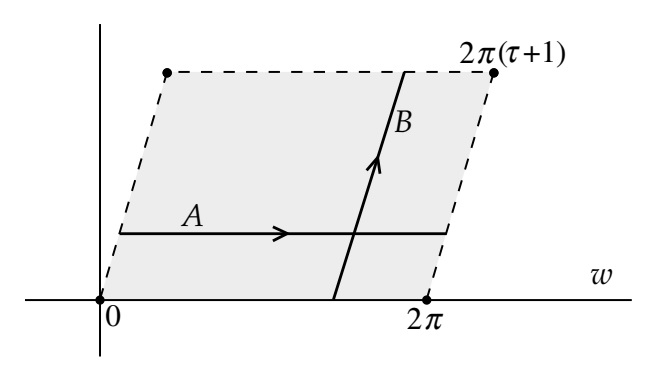
\includegraphics[width=0.5\textwidth,natwidth=490.5,natheight=276]{Fig5.1.jpg}\\
		\caption{Torus with modulus $\tau$, in gauge $d s^{2}=d w d \bar{w}$. The upper and lower edges are identified, as are the right- and left-hand edges. Closed curves $A$ and $B$ are marked for later reference.}\label{Fig5.1}
	\end{center}
\end{figure}


换一种方式,$w=\sigma^{1}+\tau \sigma^{2}$定义用$\sigma^{a}$ . 原始周期性被保留,但度规采取更普遍形式  (5.1 .9) . 对度规的积分退化到对 $\tau $ 实部和虚部的两个积分. 度规 $(5.1 .9)$ 在复共轭下不变,并且对于实的$\tau$简并,所以我们可将注意力集中在  $\operatorname{Im} \tau>0 $,正如圆的情况 $(5.1 .5)$ ,我们可以将这些参量放进度规 (5.1.9) 或周期性(5.1.11)中.参量 $\tau$ 被称为 Teichmüller参量或更普遍的模. 与点粒子不同的是,不存在类似于圆的不变长度那样的 $\tau$ 的简单不变表达式.\\
存在某些额外的冗余,其在点粒子情况没有类似物. 值 $\tau+1$ 生成了与 $\tau$相同的等价集(5.1 .11), 其中替换了 $(m, n) \rightarrow(m-n, n) $ .  $-1 / \tau$ 也是如此. 定义 $w^{\prime}=\tau w$ ,并替换 $(m, n) \rightarrow(n,-m) $ ,重复使用这两个变换
\begin{equation}
	T: \quad \tau^{\prime}=\tau+1, \quad S: \tau^{\prime}=-1 / \tau
\end{equation}
生成了
\begin{equation}
	\tau^{\prime}=\frac{a \tau+b}{c \tau+d}
\end{equation}
其中 $a, b, c, d$是满足$a d-b c=1$的整数.\\
我们也可对其进行如下考虑. 变换
\begin{equation}
	\left[\begin{array}{l}
		\sigma^{1} \\
		\sigma^{2}
	\end{array}\right]=\left[\begin{array}{ll}
		d & b \\
		c & a
	\end{array}\right]\left[\begin{array}{l}
		\sigma^{\prime 1} \\
		\sigma^{\prime 2}
	\end{array}\right]
\end{equation}
使得$\sigma$的度规(5.1 .9) 变成 $\sigma^{\prime}$的相同形式的度规,但模为$\tau^{\prime} $ ,这是环面的微分同胚映射. 由于$a d-b c=1$ ,这是一个一一映射,并保护了周期性 (5.1 .8). 然而,它无法从连续的无穷小变换从恒等变换获得————它是所谓的大坐标变换. 坐标 $\sigma$ 中的曲线A映射到 $\sigma^{\prime}$ 坐标中的曲线沿$A^{\prime}$ 方向伸长a倍,沿 $B^{\prime}$ 方向伸长c倍. 这些大坐标变换构成群 $S L(2, \mathbf{Z})$,  $\tau$ 平面上的群是 $S L(2, \mathbf{Z}) / \mathbf{Z}_{2}=$ $P S L(2, \mathbf{Z})$, 因为如果a, b, c, d符号均不变,$\tau^{\prime}$ 是不变的. 变换 $(5.1 .14)$ 的群称为模群.\\
利用模变换 (5.1.13), 可以证明每个$\tau$ 等价于区域 $F_{0}$中的一个点 ,如图(\ref{Fig5.2})所示.

\begin{figure}
	\begin{center}
		%width=0.8\textwidth,bb=0 0 729 673
		%1px=0.75pt
		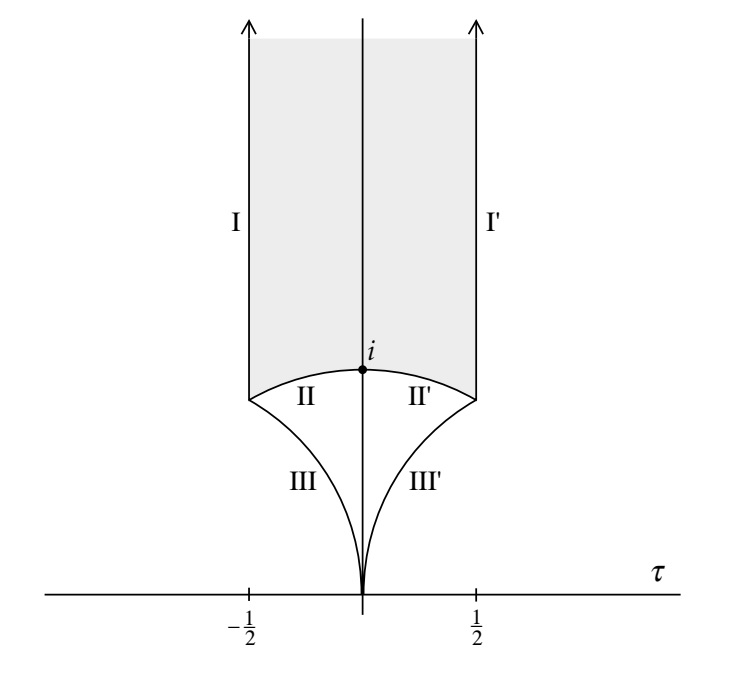
\includegraphics[width=0.5\textwidth,natwidth=546.75,natheight=504.75]{Fig5.2.jpg}\\
		\caption{The standard fundamental region $F_{0}$ for the moduli space of the torus, shaded. The lines I and I' are identified, as are the arcs II and II'. A different fundamental region, mapped into $F_{0}$ by the modular transformation $S$, is bounded by II, II', III, and III'.}\label{Fig5.2}
	\end{center}
\end{figure}

\begin{equation}
	-\frac{1}{2} \leq \operatorname{Re} \tau \leq \frac{1}{2}, \quad|\tau| \geq 1
\end{equation}
除了图中所示等价起来的边界,这被称为上半平面模掉 $\bmod P S L(2, \mathbf{Z})$的基本区域. 由于等价性,可以认为$F_{0}$ 被卷起来,仅当 $\operatorname{Im} \tau \rightarrow \infty$时开放. 基本区域 $F_{0}$ 是 ( diff $\times$ Weyl)不等价度规的模空间的一个表示.\\
对于点粒子有进一步的困难. 要求度规采取形式 (5.1.9) ,其中 $\tau$处在一个给定的基本区域,这并不固定所有的 diff $\times$ Weyl不变性. 度规以及周期性在刚性变换下不变
\begin{equation}
	\sigma^{a} \rightarrow \sigma^{a}+v^{a}
\end{equation}
所以该 diff $\times$ Weyl 二参量子群没有被固定. 另外,离散变换 $\sigma^{a} \rightarrow-\sigma^{a}$使度规不变,并且在非定向情况下$\tau \rightarrow-\bar{\tau}$的 $\left(\sigma^{1}, \sigma^{2}\right) \rightarrow\left(-\sigma^{1}, \sigma^{2}\right)$ 也使度规不变 . 因此这里又有了度规自由度与定域对称性之间的不匹配:度规中的参量不能被对称性移除,并且对称性没有被度规的选择所固定. 未固定的对称性称为共形Killing 群(C K G) .\\
当振幅中有足够多的顶点时,通过固定某些顶点算符的位置,我们可以完全固定规范不变性. 在有n个顶点算符的环面上,不变性(5.1.16) 可以用来固定一个顶点算符的位置,留下对$\tau$ 的积分,以及n-1个其他位置.  来自$\sigma^{a} \rightarrow-\sigma^{a}$ 的 $\mathbf{Z}_{2}$ 可以被要求第二个顶点算符在环面的中间固定 . 实际上,对于有限的重复计数,留下一些不固定的对称性,并除以一个合适的因子通常更方便些. 另外,如果顶点算符过少,某些共形Killing不变性仍然未固定,那么我们必须明确考虑重复计数.\\

\centerline{\Large 对读者的note}
在本章剩余部分,我们将更一般地讨论模. 主要目标是弦S矩阵的规范固定表达式 (5.3.9) . 事实上,大多数有趣的弦物理在树图振幅和一圈振幅就可以看到. 由于这个原因,测度可以通过捷径获得. 对于树图振幅,没有度规模但某些顶点算符的位置必须确定下来. 可以像(6.4.4)下面所阐述的那样推理出测度. 对于一圈振幅,通过类比(7.3.9)下面关于点粒子的讨论,可以以一种相对直观的方式理解测度. 

\section{模和Riemann面}%{5.2 Moduli and Riemann surfaces}

现在,我们以一种更普遍更抽象的方式重复之上的讨论. 我们以对某些给定拓扑 $r$上的所有度规积分. 称该度规空间为 $\mathscr{G}_{r} $ . 对于闭定向曲面,我们可以用柄的数目g,也称为亏格,来标记$r$ . 在考虑了diff $\times$ Weyl 冗余后,我们留下了模空间
\begin{equation}
	\mathscr{M}_{r}=\frac{\mathscr{G}_{r}}{(\text { diff } \times \mathrm{Weyl})_{r}}
\end{equation}
就像在环面情况那样,这个空间被有限个模参量化. 对于环面,$M_{1}$ 是上半平面模掉 $\bmod P S L(2, \mathbf{Z})$, 或等价地任意基本区域如 $F_{0}$. 还有可能存在diff $\times$ Weyl子群, 即 CKG, 使度规不变.\\
当在路径积分中有顶点算符时,用与度规中模的同等地位,看到它的位置是有用的. 当我们需要作出区分时,我们将指度规模. 一种处理CKG的方式,如果在路径积分中存在顶点算符时是适用的,是通过确定某些顶点算符的位置进一步指定规范. Polyakov路径积分包含对 $\mathscr{G}_{r}$ 的积分,以及n个顶点算符对世界面 $\mathscr{M} $的积分. 那么拓扑 $r$ 上有顶点算符的模空间是
\begin{equation}
	\mathscr{M}_{r, n}=\frac{\mathscr{G}_{r} \times M^{n}}{(\text { diff } \times \mathrm{Weyl})_{r}}
\end{equation}
就像我们在环面中看到的, $\operatorname{diff}_{r}$ 一般不是连通的. 选出包含单位元的连通部分 diff $_{r 0}$ ,商
\begin{equation}
	\frac{\operatorname{diff}_{r}}{\operatorname{diff}_{r 0}}
\end{equation}
是模群.\\
研究无限小层次上的度规的diff $\times$ Weyl冗余是很有趣的. 即,寻找一些不等价于diff $\times$ Weyl 变换的度规变分,因而等价于模中的改变. 我们也要寻找某些不改变度规的diff $\times$ Weyl 变换,这些是CKG的无限小元, 称为共形Killing矢量 ( $C K V s)$. \\
一个无限小的diff $\times$ Weyl变换对度规的改变为
\begin{equation}
	\delta g_{a b}=-2\left(P_{1} \delta \sigma\right)_{a b}+(2 \delta \omega-\nabla \cdot \delta \sigma) g_{a b}
\end{equation}
其中 $P_{1}$ 是导数的无迹对称线性组合 (3.3.17). 模所对应的度规变分 $\delta^{\prime} g_{a b}$与所有变分 (5.2 .4)正交 :
\begin{equation}
	\begin{aligned}
		0 &=\int d^{2} \sigma g^{1 / 2} \delta^{\prime} g_{a b}\left[-2\left(P_{1} \delta \sigma\right)^{a b}+(2 \delta \omega-\nabla \cdot \delta \sigma) g^{a b}\right] \\
		&=\int d^{2} \sigma g^{1 / 2}\left[-2\left(P_{1}^{T} \delta^{\prime} g\right)_{a} \delta \sigma^{a}+\delta^{\prime} g_{a b} g^{a b}(2 \delta \omega-\nabla \cdot \delta \sigma)\right]
	\end{aligned}
\end{equation}
其中平移 $\left(P_{1}^{T} u\right)_{a}=-\nabla^{b} u_{a b}$. \\

\fbox{\noindent\centering\parbox{0.9\textwidth}{注:\\
		$$
		\begin{aligned}
		(P, \delta \sigma)^{a b}&=\frac{1}{2}\left(\nabla^{a} \delta \sigma^{b}+\nabla^{b} \delta \sigma^{a}-g^{a b} \nabla \cdot \delta \sigma\right) \\
		\delta^{\prime} g_{a b}(P, \delta \sigma)^{a b}&=\frac{1}{2}\left(\delta^{\prime} g_{a b} \nabla^{a} \delta \sigma^{b}+\delta^{\prime} g_{a b} \nabla^{b} \delta \sigma^{a}-\delta^{\prime} g_{a b} g^{a b} \nabla \cdot \delta \sigma\right)
		\end{aligned}
		$$}}\\

为了使重叠(5.2 .5) 对于一般的$\delta \omega$ 与 $\delta \sigma$ 为零,我们需要
\begin{subequations}
\begin{equation}
g^{a b} \delta^{\prime} g_{a b} =0 
\end{equation}	
\begin{equation}
\left(P_{1}^{T} \delta^{\prime} g\right)_{a} =0
\end{equation}			
\end{subequations}
第一个条件要求 $\delta^{\prime} g_{a b}$ 无迹,并且是 $P_{1}^{T}$ 作用的无迹对称张量. 对于这些方程的每一解,都存在一个模.\\

CKVs 是使得 $\delta g_{a b}=0 $的(5.2 .4),该方程的迹唯一确定了 $\delta \omega$ , 留下了共形 Killing 方程
\begin{equation}
	\left(P_{1} \delta \sigma\right)_{a b}=0
\end{equation}
(5.2.6) 和 (5.2.7) 对共形规范周围的变分变得简单
\begin{subequations}
\begin{equation}
\partial_{\bar{z}} \delta^{\prime} g_{z z} =\partial_{z} \delta^{\prime} g_{\bar{z} \bar{z}}=0 
\end{equation}	
\begin{equation}
\partial_{\bar{z}} \delta z =\partial_{z} \delta \bar{z}=0
\end{equation}			
\end{subequations}
所以模的变分对应于全纯二次微分,而CKV对应全纯矢量场. 在环面上,唯一的全纯双周期函数是常数,所以存在两个实模以及两个实的CKV,与上节讨论一致.
度规模对应$P_{1}^{T}$的核(5.2 .6),而CKV对应$P_{1}$的核 (5.2 .7). Riemann-Roch定理将度规模数 $\mu=\operatorname{dim} \operatorname{ker} P_{1}^{T}$ 以及CKVs的数目$ \kappa=\operatorname{dim} \operatorname{ker} P_{1}$与Euler数 $\chi$相关联
\begin{equation}
	\mu-\kappa=-3 \chi
\end{equation}
我们将在本章后面推导它. 对于闭定向曲面 $-3 \chi=6 g-6 $ . 这个计数针对实模,将复数模例如 $\tau$ 分成了实部核虚部.
进一步,$\kappa$ 对于 $\chi<0$ 为零, $\mu$对 $\chi>0 $为零. 为证明这点,我们引用如下性质:总能通过Weyl变换找到一度规,其标量曲率 $R$ 为常数. 这样 $R$ 与 $\chi$符号相同. 现在, $P_{1}^{T} P_{1}=-\frac{1}{2} \nabla^{2}-\frac{1}{4} R$, 所以
\begin{equation}
	\begin{aligned}
		\int d^{2} \sigma g^{1 / 2}\left(P_{1} \delta \sigma\right)_{a b}\left(P_{1} \delta \sigma\right)^{a b} &=\int d^{2} \sigma g^{1 / 2} \delta \sigma_{a}\left(P_{1}^{T} P_{1} \delta \sigma\right)^{a} \\
		&=\int d^{2} \sigma g^{1 / 2}\left(\frac{1}{2} \nabla_{a} \delta \sigma_{b} \nabla^{a} \delta \sigma^{b}-\frac{R}{4} \delta \sigma_{a} \delta \sigma^{a}\right)
	\end{aligned}
\end{equation}
对于负的 $\chi$,右边是严格正定的,所以 $P_{1} \delta \sigma$ 不可能为零. 一个类似的讨论表明,对于正的 $\chi$, $P_{1}^{T} \delta^{\prime} g$不能为零. 结合这些结果,我们有
\begin{subequations}
\begin{equation}
\chi>0:  \kappa=3 \chi, \quad \mu=0 
\end{equation}
\begin{equation}
\chi<0:  \kappa=0, \quad \mu=-3 \chi
\end{equation}						
\end{subequations}

\centerline{\Large Riemann面}
描述模空间的常见方法是从每个等价类中选择一个度规,这构成依赖模$t^{k} $ 的度规族$\hat{g}_{a b}(t ; \sigma)$. 对于环面,(5.1.9) 给出这样一个切片. 使用(5.1.11)的另一描述通常比较方便, 其中 $d w d \bar{w}$ 被固定,而模被编码在坐标区域. 我们可以对这一概念进行如下形式化.\\
我们先来回忆可微流形是如何被定义的. 用一组相互交叠的集覆盖流形, $\sigma_{m}^{a}$ 是第 m个坐标卡中的坐标,而 $a$从 1取到流形的维数. 当坐标卡m与n交叠时,两个坐标卡中的坐标通过如下公式相关
\begin{equation}
	\sigma_{m}^{a}=f_{m n}^{a}\left(\sigma_{n}\right)
\end{equation}
其中要求传递函数能微分给定次. 对于 Riemannian流形,在每个坐标卡中同样给定了度规 $g_{m, a b}\left(\sigma_{m}\right)$ ,而重叠区的值通过通常的张量法则相关.\\
对于一个复流形,在每个坐标卡中存在复坐标 $z_{m}^{a}$ ,而现在a从1取到流形维数的一半. 传递函数被要求是全纯的
\begin{equation}
	z_{m}^{a}=f_{m n}^{a}\left(z_{n}\right)
\end{equation}
由于全纯性不依赖所使用的坐标 $z_{m}^{a}$. 现在可以定义流形上的全纯函数. 正如,如果两个可微流形之间存在一对一可微映射,它们就等价;如果两个复流形之间存在一对一全纯映射,它们就等价. 特别地,在每个坐标卡内做一个全纯的坐标变换,将给出等价的表面.\\
在二维情况 (一个复坐标), 复流形被称为Riemann面. 在这一情况下存在一一对应
\begin{equation}
\text{Riemann surfaces} \leftrightarrow \text{Riemannian manifolds mod Weyl}
\end{equation}
我们在右边放置了 'mod Weyl' 是因为 'mod diff' 已经隐含在 Riemannian 流形的定义中. 为了看到这个同构,从Riemannian 流形出发. 从我们对共形规范的讨论中,我们知道,可以在每个坐标卡中找到 $z_{m}$ 使得
\begin{equation}
	d s^{2} \propto d z_{m} d \bar{z}_{m}
\end{equation}
在临近的卡中,坐标不需要是相同的,但由于 $d s^{2} \propto d z_{m} d \bar{z}_{m} \propto d z_{n} d \bar{z}_{n}$, 传递函数是全纯的. 这是从Riemannian manifolds到两实维的复流形的映射. 对于逆映射,可以在第m个卡中取度规 $d z_{m} d \bar{z}_{m}$,并使其在交叠区光滑以产生Riemannian 流形. Riemann面的两个表征因而是等价的.\\
以平行四边形 (\ref{Fig5.1}) 的复坐标w来描述环面例证了复流形的思想. 假想取单个坐标卡,其比(\ref{Fig5.1}) 的基本平行四边形大一点. 那么,周期性条件
\begin{equation}
	w \cong w+2 \pi \cong w+2 \pi \tau
\end{equation}
就是坐标卡两个相反边缘的交叠上的传递函数. 这些传递函数定义了面. 为了定义原始的对度规的路径积分,将度规视为固定坐标,例如平方 (5.1.7), 或至少是传递函数固定的坐标卡的固定集合,是最简单的出发点. 为了研究给定平面上的量子场论,那么最简单的就是处理传递函数模相关的单位度规,就像平行四边形(5.1.11)中那样.\\
也可以如下看到Rieman面. 定义世界面为坐标卡的并. 我们可以用 diff $\times$ Weyl 自由度在每一坐标卡中达到度规 $d z d \bar{z}$.这样在坐标卡交叠区的规范选择只能相差该度规的diff $\times$ Weyl 不变. 这正是我们讨论过的共形变换. 因而Rieman面是CFT自然生长的地方,这是因为CFT中的场在共形变换下有明确的变换性质.

\section{模的测度}%{5.3 The measure for moduli}
我们现在回顾Polyakov路径积分的规范固定.  我们已经知道了规范冗余不完全消除对度规的路径积分,但留下了模空间上的有限维积分. 为了将其考虑在内,有必要精炼3.3节的讨论.\\
S矩阵的路径积分是
\begin{equation}
	\begin{aligned}
		&S_{j_{1} \ldots j_{n}}\left(k_{1}, \ldots, k_{n}\right) \\
		&\quad=\sum_{\begin{array}{l}
				\text { compact } \\
				\text { topologies }
		\end{array}} \int \frac{[d \phi d g]}{V_{\text {diff }} \times \text { Weyl }} \exp \left(-S_{\mathrm{m}}-\lambda \chi\right) \prod_{i=1}^{n} \int d^{2} \sigma_{i} g\left(\sigma_{i}\right)^{1 / 2} \mathscr{V}_{j_{i}}\left(k_{i}, \sigma_{i}\right)
	\end{aligned}
\end{equation}
这是之前的表达式(3.5.5) ,但现在有一个$c=\tilde{c}=26$ 的普遍物质场,物质场用 $\phi $标记. 在规范固定中,对度规和位置的积分换成对规范群、模以及未定位置的积分
\begin{equation}
	[d g] d^{2 n} \sigma \rightarrow[d \zeta] d^{\mu} t d^{2 n-\kappa} \sigma
\end{equation}
在因式分解出规范体积后,这一变换的Jacobian行列式就变成了模空间上的测度.\\
这一步与3.3节是相同的,现在将模与CKV考虑在内.特别地,规范选择现在会固定 $\kappa$ 个顶点坐标, $\sigma_{i}^{a} \rightarrow \hat{\sigma}_{i}^{a} $ . 记固定坐标 $(a, i)$ 的集合为 $f $ ,定义模空间上的Faddeev-Popov测度为
\begin{equation}
	1=\Delta_{\mathrm{FP}}(g, \sigma) \int_{F} d^{\mu} t \int_{\mathrm{diff} \times \mathrm{Weyl}}[d \zeta] \delta\left(g-\hat{g}(t)^{\zeta}\right) \prod_{(a, i) \in f} \delta\left(\sigma_{i}^{a}-\hat{\sigma}_{i}^{\zeta a}\right)
\end{equation}
通过定义,每个度规 (diff $\times$ Weyl)等价于一个$t$ and $\zeta $的$\hat{g}(t)$ . 实际上,正如5.1节末尾所讨论的,可能会存在一个残留的有限阶 $n_{R}$的离散对称群,所以delta函数在$n_{R}$个点非零.\\
将(5.3.3) 代入路径积分 (5.3.1) ,并使用与之前相同步骤给出
\begin{equation}
	\begin{aligned}
		S_{j_{1} \ldots j_{n}}\left(k_{1}, \ldots, k_{n}\right)=& \sum_{\text {compact },\text { topologies } } \int_{F} d^{\mu} t \Delta_{\mathrm{FP}}(\hat{g}(t), \hat{\sigma}) \int[d \phi] \int \prod_{(a, i) \notin f} d \sigma_{i}^{a} \\	
		&\times \exp \left(-S_{\mathrm{m}}[\phi, \hat{g}(t)]-\lambda \chi\right) \prod_{i=1}^{n}\left[\hat{g}\left(\sigma_{i}\right)^{1 / 2} \mathscr{N}_{j_{i}}\left(k_{i} ; \sigma_{i}\right)\right]
	\end{aligned}
\end{equation}
对度规和顶点算符坐标的积分现在退化成对度规和未定坐标的模空间 $F$加上 $\Delta_{\mathrm{FP}} $ 给定的测度的积分. 在顶点算符中,$\kappa$个位置被固定了.\\
现在我们计算Faddeev-Popov测度. delta函数在对称相关的 $n_{R}$个点上非零,所以我们考察一个这样的点并除以$n_{R} $ . 在该点附近展开$\Delta_{\mathrm{FP}}$的定义(5.3 .3). 一般度规变分等于定域对称变分加上模 $t^{k}$的一个变化,
\begin{equation}
	\delta g_{a b}=\sum_{k=1}^{\mu} \delta t^{k} \partial_{t^{k}} \hat{g}_{a b}-2\left(\hat{P}_{1} \delta \sigma\right)_{a b}+(2 \delta \omega-\hat{\nabla} \cdot \delta \sigma) \hat{g}_{a b}
\end{equation}
Faddeev-Popov逆行列式为
\begin{equation}
	\begin{aligned}
		&\Delta_{\mathrm{FP}}(\hat{g}, \hat{\sigma})^{-1} \\
		&=n_{R} \int d^{\mu} \delta t[d \delta \omega d \delta \sigma] \delta\left(\delta g_{a b}\right) \prod_{(a, i) \in f} \delta\left(\delta \sigma^{a}\left(\hat{\sigma}_{i}\right)\right)\\
		&=n_{R}  \int d^{\mu} \delta t d^{\kappa} x\left[d \beta^{\prime} d \delta \sigma\right] \\
		&\quad \times \exp \left[2 \pi i\left(\beta^{\prime}, 2 \hat{P}_{1} \delta \sigma-\delta t^{k} \partial_{k} \hat{g}\right)+2 \pi i \sum_{(a, i) \in f} x_{a i} \delta \sigma^{a}\left(\hat{\sigma}_{i}\right)\right]
	\end{aligned}
\end{equation}
第二行中内积的定义参考习题3.2. 我们跟随了与3.3节相同的定域讨论,将delta函数与泛函写成对$x$ 与 $\beta_{a b}$ 的积分,并积掉 $\delta \omega$ 以获得 $\beta_{a b}^{\prime}$ 是无迹的约束.\\
像之前一样,将所有bosonic变量替换成Grassmann变量来转换积分(5.3 .6):
\begin{subequations}
\begin{equation}
\delta \sigma^{a}  \rightarrow c^{a} 
\end{equation}
\begin{equation}
\beta_{a b}^{\prime}  \rightarrow b_{a b} 
\end{equation}
\begin{equation}
x_{a i}  \rightarrow \eta_{a i} 
\end{equation}
\begin{equation}
\delta t^{k}  \rightarrow \xi^{k}
\end{equation}	
\end{subequations}
然后,在场的传统归一化下
\begin{equation}
	\begin{aligned}
		\Delta_{\mathrm{FP}}(\hat{\mathrm{g}}, \hat{\sigma})=& \frac{1}{n_{R}} \int[d b d c] d^{\mu} \xi d^{\kappa} \eta \\
		&\quad \times \exp \left[-\frac{1}{4 \pi}\left(b, 2 \hat{P}_{1} c-\xi^{k} \partial_{k} \hat{g}\right)+\sum_{(a, i) \in f} \eta_{a i} c^{a}\left(\hat{\sigma}_{i}\right)\right] \\
		=& \frac{1}{n_{R}} \int[d b d c] \exp \left(-S_{\mathrm{g}}\right) \prod_{k=1}^{\mu} \frac{1}{4 \pi}\left(b, \partial_{k} \hat{g}\right) \prod_{(a, i) \in f} c^{a}\left(\hat{\sigma}_{i}\right)
	\end{aligned}
\end{equation}
在最后一行,我们积掉了Grassmann 变量 $\eta_{a i}$和 $\xi^{k}$.\\
模空间上合适的积分测度由带有该插入鬼路径积分生成. 我们不试图在中间步骤保留总符号的踪迹;既然这是一个Jacobian行列式,我们可以暗中选择总符号以给出正的结果. S矩阵的完整表达式是
\begin{equation}
	\begin{aligned}
		&S_{j_{1} \ldots j_{n}}\left(k_{1}, \ldots, k_{n}\right)\\
		&=\sum_{\text {compact },\text { topologies }} \int_{F} \frac{d^{\mu} t}{n_{R}} \int[d \phi d b d c] \exp \left(-S_{\mathrm{m}}-S_{\mathrm{g}}-\lambda \chi\right) \\
		&\times \prod_{(a, i) \notin f} \int d \sigma_{i}^{a} \prod_{k=1}^{\mu} \frac{1}{4 \pi}\left(b, \partial_{k} \hat{g}\right) \prod_{(a, i) \in f} c^{a}\left(\hat{\sigma}_{i}\right) \prod_{i=1}^{n} \hat{g}\left(\sigma_{i}\right)^{1 / 2} \mathscr{V}_{j_{i}}\left(k_{i}, \sigma_{i}\right)
	\end{aligned}
\end{equation}
这一结果随时可以扩展到所有bosonic弦理论 - 闭的或开的,定向或非定向的-唯一的差异是要纳入什么样的拓扑并允许什么样的顶点算符. Eq. (5.3.9) 是一个有用且漂亮的结果. 模和CKV引入的复杂性通过在路径积分中插入b和c而考虑在内. 对于每个固定坐标, $d \sigma_{i}^{a}$被替换成 $c_{i}^{a}$, 而每个度规模给出b插入.

\centerline{\Large 行列式形式的表示}
在 (5.3.8) 中,我们将Faddeev-Popov行列式表示成对Grassmann变量和场的积分.我们现在要将其化简成有限维泛函行列式的乘积. 当我们在接下来的章节中继续研究弦S矩阵时,这一直接的路径积分方法仅是我们要使用的方法之一.\\
在合适的完备基下展开鬼场
\begin{equation}
	c^{a}(\sigma)=\sum_{J} c_{J} \mathrm{C}_{J}^{a}(\sigma), \quad b_{a b}(\sigma)=\sum_{K} b_{K} \mathrm{~B}_{K a b}(\sigma)
\end{equation}
完备基 $C_{J}^{a}$ 与 $B_{K a b}$定义如下. 出现在鬼作用量中的导数 $P_{1}$ 将矢量转换成无迹对称张量. 而它的转置是相反的功能. 鬼作用量可以写成
\begin{equation}
	S_{\mathrm{g}}=\frac{1}{2 \pi}\left(b, P_{1} c\right)=\frac{1}{2 \pi}\left(P_{1}^{T} b, c\right)
\end{equation}
我们无法以一种diff不变的方式对角化 $P_{1}$,因为它将一种场转化成另一种,但我们可以对角化$P_{1}^{T} P_{1}$ 和 $P_{1} P_{1}^{T}$:
\begin{equation}
	P_{1}^{T} P_{1} \mathrm{C}_{J}^{a}=v_{J}^{\prime 2} \mathrm{C}_{J}^{a}, \quad P_{1} P_{1}^{T} \mathrm{~B}_{K a b}=v_{K}^{2} \mathrm{~B}_{K a b}
\end{equation}
本征函数可以选为实的,并在如下内积中归一化
\begin{subequations}
\begin{equation}
\left(\mathrm{C}_{J}, \mathrm{C}_{J^{\prime}}\right) =\int d^{2} \sigma g^{1 / 2} \mathrm{C}_{J}^{a} \mathrm{C}_{J^{\prime} a}=\delta_{J J^{\prime}} 
\end{equation}
\begin{equation}
\left(\mathrm{B}_{K}, \mathrm{~B}_{K^{\prime}}\right) =\int d^{2} \sigma g^{1 / 2} \mathrm{~B}_{K a b} \mathrm{~B}_{K^{\prime}}^{a b}=\delta_{K K^{\prime}}
\end{equation}
\end{subequations}
现在注意到
\begin{equation}
	\left(P_{1} P_{1}^{T}\right) P_{1} \mathrm{C}_{J}=P_{1}\left(P_{1}^{T} P_{1}\right) \mathrm{C}_{J}=v_{J}^{\prime 2} P_{1} \mathrm{C}_{J}
\end{equation}
所以 $P_{1} \mathrm{C}_{J}$是 $P_{1} P_{1}^{T} $的本征函数. 以同样方法, $P_{1}^{T} \mathrm{~B}_{K}$ 是 $P_{1}^{T} P_{1} $的本征函数. 因此除了 $P_{1} \mathrm{C}_{J}=0$ 或 $P_{1}^{T} \mathrm{~B}_{K}=0 $,本征函数之间存在一一映射.  它们对应 $P_{1}^{T} P_{1}$ 或 $P_{1} P_{1}^{T} $的本征值. 它们正是CKV和全纯二次微分,因而它们的数目分别是 $\kappa$ 和 $\mu$. 我们将零本征值的本征函数记为 $\mathrm{C}_{0 j}$ 或$\mathrm{B}_{0 k}$, 而非零本征值被标记为 $J, K=1, \ldots$ . 对于后者,归一化关联函数的关联为
\begin{equation}
	\mathrm{B}_{J a b}=\frac{1}{v_{J}}\left(P_{1} \mathrm{C}_{J}\right)_{a b}, \quad v_{J}=v_{J}^{\prime} \neq 0
\end{equation}
以模的形式,鬼路径积分 $\Delta_{\mathrm{FP}}$ 变成
\begin{equation}
	\int \prod_{k=1}^{\mu} d b_{0 k} \prod_{j=1}^{\kappa} d c_{0 j} \prod_{J} d b_{J} d c_{J} \exp \left(-\frac{v_{J} b_{J} c_{J}}{2 \pi}\right) \prod_{k^{\prime}=1}^{\mu} \frac{1}{4 \pi}\left(b, \partial_{k^{\prime}} \hat{g}\right) \prod_{(a, i) \in f} c^{a}\left(\sigma_{i}\right)
\end{equation}
从A.2节,我们知道,除非变量出现在被积函数中,否则Grassmann积分为零. $c_{0 j}$ 和 $b_{0 k}$ 没有出现在作用量中,而仅仅出现在插入中. 事实上,积分(5.3 .16)中每一种插入的数目,$ \kappa$ 和 $\mu$ ,分别与鬼零模匹配. 我们恰好有足够多的插入以给出非零的结果,并且在插入中,只有鬼场的零模部分有贡献. 因此
\begin{equation}
	\begin{aligned}
		\Delta_{\mathrm{FP}}=\int \prod_{k=1}^{\mu} & d b_{0 k} \prod_{k^{\prime}=1}^{\mu}\left[\sum_{k^{\prime \prime}=1}^{\mu} \frac{b_{0 k^{\prime \prime}}}{4 \pi}\left(\mathrm{B}_{0 k^{\prime \prime}}, \partial_{k^{\prime}} \hat{g}\right)\right] \\
		& \times \int \prod_{j=1}^{\kappa} d c_{0 j} \prod_{(a, i) \in f}\left[\sum_{j^{\prime}=1}^{\kappa} c_{0 j^{\prime}} \mathrm{C}_{0 j^{\prime}}^{a}\left(\sigma_{i}\right)\right] \\
		& \times \int \prod_{J} d b_{J} d c_{J} \exp \left(-\frac{v_{J} b_{J} c_{J}}{2 \pi}\right)
	\end{aligned}
\end{equation}
对所有使得零模积分充满Grassmann变量的方式求和,在每种情况下,积分会生成有限行列式,而非零模产生一个无穷乘积,一个泛函行列式. 合起来
\begin{equation}
	\Delta_{\mathrm{FP}}=\operatorname{det} \frac{\left(\mathrm{B}_{0 k}, \partial_{k^{\prime}} \hat{g}\right)}{4 \pi} \operatorname{det} C_{0 j}^{a}\left(\sigma_{i}\right) \operatorname{det}^{\prime}\left(\frac{P_{1}^{T} P_{1}}{4 \pi^{2}}\right)^{1 / 2}
\end{equation}
注意到$\mathrm{C}_{0 j}^{a}\left(\sigma_{i}\right)$ 是平方矩阵,其中 $(a, i) \in f$ 像j一样取遍 $\kappa$ 个值.泛函行列式上的撇代表去掉了零本征值.\\

\centerline{\Large Riemann- Roch定理}
我们现在给出Riemann-Roch 定理的一个路径积分推导.对于全纯 $b c$ 系统 (没有 $\tilde{b}, \tilde{c}$)的鬼流, 习题3.6中导出的流守恒反常是
\begin{equation}
	\nabla_{a} j^{a}=\frac{1-2 \lambda}{4} R
\end{equation}
Noether定理将流守恒与不变性相关联. 对于不守恒流,通过讨论发现
\begin{equation}
	\frac{\delta([d \phi] \exp (-S))}{[d \phi] \exp (-S)}=\frac{i \epsilon}{2 \pi} \int d^{2} \sigma g^{1 / 2} \nabla_{a} j^{a} \rightarrow-i \epsilon \frac{2 \lambda-1}{2} \chi
\end{equation}
鬼数对称性的作用为 $\delta b=-i \epsilon b, \delta c=i \epsilon c $.  当路径积分非零时,测度、作用量和插入的变换必须相互抵消. 因此,从反常中我们了解到c插入的数目减去b插入的数目是$3 \chi / 2 $.  路径积分计算将插入的数目与零模的数目关联起来,因而给出相同的差值
\begin{equation}
	\frac{1}{2}(\kappa-\mu)=\frac{1}{2}\left(\operatorname{dim} \operatorname{ker} P_{1}-\operatorname{dim} \operatorname{ker} P_{1}^{T}\right)
\end{equation}
因子 $\frac{1}{2}$的出现是因为我们仅仅取出了全纯理论,反全纯理论给出相同贡献. 等同从反常中得到的结果与从零模中得到的结果给出Riemann-Roch 定理 $\kappa-\mu=3 \chi$. 对一般的$b c$系统,以相同方式会发现
\begin{equation}
	\operatorname{dim} \operatorname{ker} P_{n}-\operatorname{dim} \operatorname{ker} P_{n}^{T}=(2 n+1) \chi
\end{equation}
$P_{n}$算符在习题3.2中定义.

\section{关于测度的更多介绍}%{5.4 More about the measure}
这里我们收集了一些规范固定弦振幅的普遍性质. 它们对于第9章中的更加形式化的考察由奠基性的作用.\\

\centerline{\Large 规范不变性}
Faddeev-Popov处理所生成的规范固定振幅是BRST不变且独立于规范选择. 然而,明确的检验它是否有期望的全部性质是很有用的. \\
第一,它独立于模空间上坐标t的选择. 对于新坐标$t^{\prime k}(t)$
\begin{equation}
	\begin{aligned}
		d^{\mu} t^{\prime} &=\left|\operatorname{det} \frac{\partial t^{\prime}}{\partial t}\right| d^{\mu} t \\
		\prod_{k=1}^{\mu} \frac{1}{4 \pi}\left(b, \partial_{k}^{\prime} \hat{g}\right) &=\operatorname{det}\left(\frac{\partial t}{\partial t^{\prime}}\right) \prod_{k=1}^{\mu} \frac{1}{4 \pi}\left(b, \partial_{k} \hat{g}\right)
	\end{aligned}
\end{equation}
并且这两个Jacobians行列式相互抵消 (相差一个符号,我们会手动决定以给出一个正的测度). 换句话说,b鬼引起的积分像模空间上的密度那样变换.\\
第二,我们来看一下该测度在规范切片的Weyl变换下不变. 在Weyl变换下,
\begin{equation}
	\delta \hat{g}_{a b}^{\prime}(t ; \sigma)=2 \delta \omega(t ; \sigma) \hat{g}_{a b}(t ; \sigma)
\end{equation}
作用量和测度的变分给出了定域算符$T_{a}^{a}$的插入,其在 $D=26$ 由于运动方程而为零. 因而,我们只需要关心各个插入上的效应. 顶点算符插入由于收缩进而为零.插入 $c^{a}\left(\sigma_{i}\right)$ 根据 (3.3.24)下面的讨论而为零. 对于
\begin{equation}
	\begin{aligned}
		\left(b, \partial_{k} \hat{g}^{\prime}\right) &=\int d^{2} \sigma \hat{g}^{\prime 1 / 2} b_{a b} \hat{g}^{\prime a c} \hat{g}^{b d} \partial_{k} \hat{g}_{c d}^{\prime} \\
		&=\int d^{2} \sigma \hat{g}^{1 / 2} b_{a b}\left(\hat{g}^{a c} \hat{g}^{b d} \partial_{k} \hat{g}_{c d}+2 \hat{g}^{a b} \partial_{k} \omega\right) \\
		&=\left(b, \partial_{k} \hat{g}\right)
	\end{aligned}
\end{equation}
最后一个等式由于 $b$的无迹而成立.\\
第三,我们来检验无限小diff变换 $\delta \sigma=\xi(t ; \sigma) $下的不变性.  扩展到一般diff变换是直接的. 振幅(5.3.9)中唯一一个不是立即不变的项是b插入以及坐标被固定的顶点算符. 前者变换为
\begin{equation}
	\begin{aligned}
		\delta\left(b, \partial_{k} \hat{g}\right) &=-2\left(b, P_{1} \partial_{k} \xi\right) \\
		&=-2\left(P_{1}^{T} b, \partial_{k} \xi\right) \\
		&=0
	\end{aligned}
\end{equation}
其中利用了b的运动方程. b运动方程来自$\delta S / \delta c=0$,所以在c插入上会存在源项; 它们是解释坐标变换在固定顶点算符上的效应所需要的.\\

\centerline{\Large BRST不变性}
我们现在来证明(5.3 .9)的全BRST不变性 . 从定域分析中知道路径积分测度与作用量是不变的,所以我们不得不考察BRST变换在插入上的效应. 在规范固定路径积分(5.3.9)中,非定向顶点算符伴随着因子 $c$ 或 $\tilde{c} c$. 这是我们在4.4节末尾对对应于OCQ态的BRST不变顶点算符的描述. 另一方面,被积顶点算符不是BRST不变的,它们有BRST性质:
\begin{equation}
	\delta_{\mathrm{B}} \mathscr{V}_{\mathrm{m}}=i \epsilon \partial_{a}\left(c^{a} \mathscr{V}_{\mathrm{m}}\right)
\end{equation}
其在积分意义下为零.最终还有b插入的变分
\begin{equation}
	\delta_{\mathrm{B}}\left(b, \partial_{k} \hat{g}\right)=i \epsilon\left(T, \partial_{k} \hat{g}\right)
\end{equation}
能动量张量的插入仅产生了对$t^{k}$的导数,所以除了一个可能来自于模空间边界的项,BRST变分为零. 在下一章巡航,我们将检验模空间的边界. 在大多数情况不存在表面贡献,这是由于所谓的抵消传播子讨论. 在一定情形下,这个讨论并不适用,我们将看到如何处理这一点.\\
重要的是,规范固定结果(5.3 .9)可以直接从BRST不变性的要求写出来,而不用参考规范固定形式.正如我们在计算路径积分时候看到的,至少存在 $\mu $ 个b插入和 $\kappa $ 个c插入,否则路径积分为零. 在振幅(5.3.9)中正好存在数目正确的鬼插入以给出非零结果. 一旦我们引入必需的b因子,BRST变换在能动张量中带来与度规的$t^{k}$ 导数的卷积. 这正比于对模的导数,所以我们就像以前做的那样,对模空间积分就得到了一个不变的结果. 结果(5.3 .9)可以以各种方式推广. (例如共形Killing不变情况是保持不固定). 在第7章,对于无顶点算符的环面,我们将明确地例证这一点.BRST不变性暗示了BRST等价态的振幅是相同的. 如果我们给任意一个态增加一个空部分$Q_{B}|\chi\rangle$,效果是在路径积分中插入变分 $\delta_{B} \mathscr{V}_{\chi} $ ;这个积分为零. 这是重要的,因为物理Hilbert空间等同为上同调,所以等价态应该有相同振幅.\\

\centerline{\Large Riemann面的测度}
我们在规范固定世界面是由模-相关度规导出的框架中推导出了Faddeev-Popov测度.我们现在在Riemann面的框架中重铸这个结果,在这个框架中,结构被编码进入模相关传递函数中.\\
为了表示该测度在模空间中给定点$t_{0}$ 处的值,我们取一组坐标卡,在第m坐标卡有复坐标 $z_{m}$,以及全纯的传递函数,其中度规 $\hat{g}\left(t_{0}\right)$ 在每个坐标卡中等价于$d z_{m} d \bar{z}_{m}$ . 现在考察模的变化. 我们先将其描述为传递函数固定的度规中的变换,然后将其转化为度规固定的传递函数的变化. 在第一种描述中,定义Beltrami微分
\begin{equation}
	\mu_{k a}^{b}=\frac{1}{2} \hat{g}^{b c} \partial_{k} \hat{g}_{a c}
\end{equation}
 $\delta t^{k}$ 的b插入变成
\begin{equation}
	\frac{1}{2 \pi}\left(b, \mu_{k}\right)=\frac{1}{2 \pi} \int d^{2} z\left(b_{z z} \mu_{k \bar{z}}^{z}+b_{\bar{z} \bar{z}} \mu_{k z}^{\bar{z}}\right)
\end{equation}
在第二种描述中,在模中的变换 $\delta t^{k}$ 之后,在每个坐标卡中将会有新坐标
\begin{equation}
	z_{m}^{\prime}=z_{m}+\delta t^{k} v_{k m}^{z_{m}}\left(z_{m}, \bar{z}_{m}\right)
\end{equation}
$v_{k m}^{a}$ 上的上标是顶点指标;注意到 $v_{k m}^{a}$仅定义在第m个坐标卡中. 通过 Riemann 面的定义, $d z_{m}^{\prime} d \bar{z}_{m}^{\prime}$ 等价于 $t_{0}+\delta t$处的度规
\begin{equation}
	d z_{m}^{\prime} d \bar{z}_{m}^{\prime} \propto d z_{m} d \bar{z}_{m}+\delta t^{k}\left(\mu_{k z_{m}}^{\bar{z}_{m}} d z_{m} d z_{m}+\mu_{k \bar{z}_{m}}^{z_{m}} d \bar{z}_{m} d \bar{z}_{m}\right)
\end{equation}
因此坐标变化 $v_{k m}^{a}$与Beltrami微分的关系为
\begin{equation}
	\mu_{k z_{m}}^{\overline{\bar{z}}_{m}}=\partial_{z_{m}} v_{k m}^{\bar{z}_{m}}, \quad \mu_{k \bar{z}_{m}}^{z_{m}}=\partial_{\bar{z}_{m}} v_{k m}^{z_{m}}
\end{equation}
这是Beltrami方程的无穷小版本. 它暗示了$v_{k m}^{z_{m}}$ 不是全纯的,否则它将不对应模的变化.另外, $v_{k m}^{z_{m}}$ 中有一个不由Beltrami方程决定的全纯部分,对于 $v_{k m}^{\bar{z}_{m}}$则是反全纯部分;这些对应于每个坐标卡中做全纯再参量化的自由度.\\
分部积分,b插入 (5.4 .8)变成
\begin{equation}
	\frac{1}{2 \pi}\left(b, \mu_{k}\right)=\frac{1}{2 \pi i} \sum_{m} \oint_{C_{m}}\left(d z_{m} v_{k m}^{z_{m}} b_{z_{m} z_{m}}-d \bar{z}_{m} v_{k m}^{\bar{z}_{m}} b_{\bar{z}_{m} \bar{z}_{m}}\right)
\end{equation}
围道 $C_{m}$ 逆时针围绕第m个坐标卡. 通过(5.4.9),坐标对模的导数在给定点是
\begin{equation}
	\frac{d z_{m}}{d t^{k}}=v_{k m}^{z_{m}}
\end{equation}
因此,传递函数在模变换下的变换是
\begin{equation}
	\left.\frac{\partial z_{m}}{\partial t^{k}}\right|_{z_{n}}=v_{k m}^{z_{m}}-\frac{\partial z_{m}}{\partial z_{n}} \mid v_{t}^{z_{k n}}=v_{k m}^{z_{m}}-v_{k n}^{z_{m}}
\end{equation}
那么,结合环绕邻近坐标卡的围道积分 (5.4.12)给出
\begin{equation}
	\frac{1}{2 \pi}\left(b, \mu_{k}\right)=\frac{1}{2 \pi i} \sum_{(m n)} \int_{C_{m n}}\left(\left.d z_{m} \frac{\partial z_{m}}{\partial t^{k}}\right|_{z_{n}} b_{z_{m} z_{m}}-\left.d \bar{z}_{m} \frac{\partial \bar{z}_{m}}{\partial t^{k}}\right|_{z_{n}} b_{\bar{z}_{m} \bar{z}_{m}}\right)
\end{equation}
这正比于传递函数的导数. 求和取遍所有重叠的坐标卡. 围道 $C_{m n}$ 在卡$m$ 和 $n$之间跑动, 并在方向在$m$的视角下是逆时针的.   $(m n)$ 项关于 $m$ 和 $n$对称,但这并不显然. 每个围道要么闭合,要么在坐标卡 $m, n$和 $p$重合区域截止,在这里围道 $C_{m n}, C_{n p}$和$C_{p m}$ 交于一点.b插入现在以定义Riemann面的数据显式地表述出来,传递函数模掉了全纯等价性.\\
作为一个例证,我们可以用其将度规的模与顶点算符位置的模放在一个更加平等的基础上. 考察坐标系z中处于$z_{v}$ 处的顶点算符. 以顶点算符为中心做一个较小的新坐标卡 $z^{\prime}$, 如图(\ref{Fig5.3})所示. 

\begin{figure}
	\begin{center}
		%width=0.8\textwidth,bb=0 0 436 415
		%1px=0.75pt
		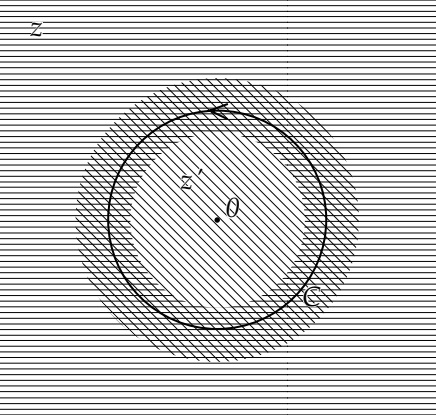
\includegraphics[width=0.5\textwidth,natwidth=327,natheight=311]{Fig5.3.jpg}\\
		\caption{Coordinate patches $z^{\prime}$ (diagonal hatching) and $z$ (horizontal hatching) with vertex operator at $z^{\prime}=0$. In the annular region, $z=z^{\prime}+z_{v}$.}\label{Fig5.3}
	\end{center}
\end{figure}

我们保留$z^{\prime}=0$处的顶点算符, 并将它的位置编码进传递函数中
\begin{equation}
	z=z^{\prime}+z_{v}
\end{equation}
 $z_{v}, \bar{z}_{v}$ 的测度由(5.4 .15)给定,其中
\begin{equation}
	\left.\frac{\partial z^{\prime}}{\partial z_{v}}\right|_{z}=-1
\end{equation}
因此,鬼插入是
\begin{equation}
	\int_{C} \frac{d z^{\prime}}{2 \pi i} b_{z^{\prime} z^{\prime}} \int_{C} \frac{d \bar{z}_{m}^{\prime}}{-2 \pi i} b_{\bar{z}^{\prime} \bar{z}^{\prime}}=b_{-1} \tilde{b}_{-1} \cdot
\end{equation}
其中 $C$ 是如图所示环绕顶点算符的任意围道.那么,S矩阵的完整表达式可以紧凑的写成
\begin{equation}
	S(1 ; \ldots ; n)=\sum_{\begin{array}{c}
			\text { compact } \atop \text { topologies }
	\end{array}} e^{-\lambda \chi} \int_{F} \frac{d^{m} t}{n_{R}}\left\langle\prod_{k=1}^{m} B_{k} \prod_{i=1}^{n} \hat{\mathscr{V}}_{i}\right\rangle
\end{equation}
这里, $B_{k}$ 是b鬼插入 (5.4 .15)的简写,而$\hat{\hat{V}}$ 对于闭弦代表 $\tilde{c} c \mathscr{K}_{\mathrm{m}}$,对于开弦代表 $t_{a} c^{a} \mathscr{\psi}_{\mathrm{m}}$. 即,我们现在将所有的顶点算符处理成固定的,并将它们的坐标换成传递函数中的额外参量.模的数目m是
\begin{equation}
	m=\mu+2 n_{\mathrm{c}}+n_{\mathrm{o}}-\kappa=-3 \chi+2 n_{\mathrm{c}}+n_{\mathrm{o}}
\end{equation}
其中 $n_{\mathrm{c}}$ 和 $n_{\mathrm{o}}$ 分别是闭弦顶点算符和开弦顶点算符的数目.\\
(5.4.19) 表明了戴帽的顶点算符,即含有 $\tilde{c} c$ 或 $t_{a} c^{a}$, 的算符是基础的. 这正是态-算符对应所产生的,并且它是BRST不变的. 如果顶点算符被积分了,鬼插入(5.4.18) 会移除$\tilde{c} c$或 $t_{a} c^{a} $ . 例如
\begin{equation}
	b_{-1} \tilde{b}_{-1} \cdot \tilde{c} c \mathscr{V}_{\mathrm{m}}=\mathscr{V}_{\mathrm{m}}
\end{equation}
留下了顶点算符的积分形式. 我们从Polyakov路径积分中写出 (5.4.19),所以顶点算符以OCQ的形式出现,但现在我们可以使用任意的BRST不变顶点算符.


% \setcounter{section}{0}%更改chapter的计数器值
% %\numberwithin{equation}{chapter}%公式计数器从属于节计数器
% \numberwithin{equation}{section}%公式计数器从属于节计数器
% \numberwithin{figure}{section}%图计数器从属于节计数器
% \setcounter{chapter}{5}

%\chapter{\texorpdfstring{树图振幅}{6 Tree-level amplitudes}}
\chapter{树图振幅} \label{cha:6}
我们现在来研究弦相互作用. 在本章, 我们将考察最低阶振幅, 他们来源于欧拉数为正的面, 我们首先描述相关的黎曼面并计算所需要的 CFT 期望值.
接下来我们将研究散射振幅, 首先是开弦, 然后是闭弦. 沿着这条路, 我们在开弦理论中会引入一个重要的推广: Chan-Paton因子. 
在本节末尾我们将回到 CFT, 并讨论期望值的普遍性质.
%\section{\texorpdfstring{Riemann面}{6.1 Riemann surfaces}}

\section{黎曼面} \label{sec:6.1}

欧拉数为正的黎曼面有三种: 球面, 圆盘以及投影平面.

\subsection*{球面}

\begin{figure}
	\begin{center}
		%width=0.8\textwidth,bb=0 0 545 585
		%1px=0.75pt
		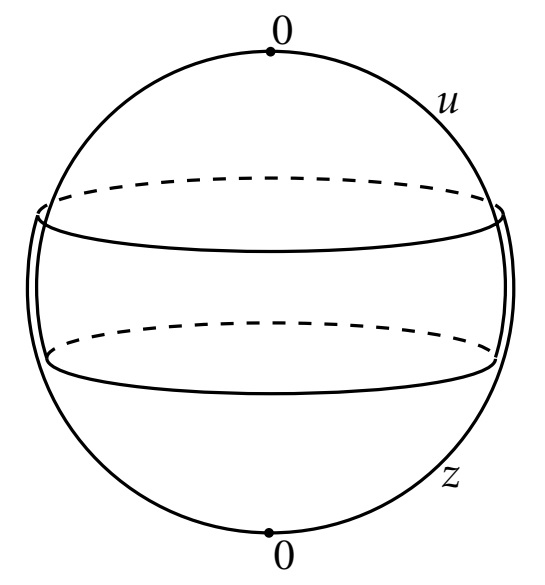
\includegraphics[width=0.5\textwidth,natwidth=408.75,natheight=438.75]{Fig6.1.jpg}\\
		\caption{从$z$坐标卡和$u$坐标卡构建的球面}\label{fig:6.1}
	\end{center}
\end{figure}

球面$S_2$可以被两个坐标卡覆盖, 如图\ref{fig:6.1}所示. 取圆盘$|z|<\rho$ 以及 $|u|<\rho$, 其中 $\rho>1$, 
并通过 
\begin{equation}
u=1 / z  \label{6.1.1}
\end{equation}
来做粘合. 事实上, 我们可以取 $\rho \to \infty$. 这样, 坐标 $z$在``北极''点$u=0$处都是良好的. 

我们可以认为球面是黎曼面, 在两个坐标卡上均取平坦度规, 并用一个共形(坐标加 Weyl)变换连接两个坐标卡. 
或者我们可以将其视为有一个整体定义的度规的黎曼流形. 一般的共形规范度规是
\begin{equation}
	\dif s^{2}=\exp (2 \omega(z, \bar{z})) \dif z \dif \bar{z} \:. \label{6.1.2}
\end{equation}
由于 $\dif z \dif \bar{z}=|z|^{4} \dif u \dif \bar{u}$, 这一度规在$u=0$不奇异的条件是$\exp (2 \omega(z, \bar{z}))$ 在 $z \to \infty $按 $|z|^{-4}$衰减. 例如,
\begin{equation}
	\dif s^{2}=\frac{4 r^{2}\, \dif z \dif \bar{z}}{(1+z \bar{z})^{2}}=\frac{4 r^{2}\, \dif u \dif \bar{u}}{(1+u \bar{u})^{2}} \label{6.1.3}
\end{equation}
描述了半径为 $r$, 曲率为 $R=2 / r^{2}$的球面.

根据\ref{sec:5.2}节的普遍讨论, 球面没有模但有6个CKV, 使得每个度规 (diff $\times$ Weyl)等价于\eqref{6.1.3}. 
我们在无限小层次观察这一点. 正如在\eqref{5.2.8}寻找的是全纯张量场$\delta g_{z z}(z)$ 和全纯矢量场 $\delta z(z)$. 
这些必须定义在整个球面上, 所以我们要考察到$u$坐标卡的变换
\begin{subequations}  \label{6.1.4}
	\begin{align}
		\delta u &=\frac{\partial u}{\partial z} \delta z=-z^{-2} \delta z \:, \label{6.1.4a} \\
		\delta g_{u u} &=\left(\frac{\partial u}{\partial z}\right)^{-2} \delta g_{z z}=z^{4} \delta g_{z z} \:. \label{6.1.4b} 
	\end{align}
\end{subequations}
任何全纯二次微分 $\delta g_{z z}$ 必须关于 $z$ 全纯, 并且在无穷远处以 $z^{-4}$ 趋于零, 因而必须恒等于零. 
另一方面, $\mathrm{CKV} \delta z$在 $u=0$全纯使得它在 $z \rightarrow \infty$增长不超过 $z^{2}$. 那么一般的 $\mathrm{CKV}$ 是
\begin{subequations} \label{6.1.5}
	\begin{align}
		\delta z       &= a_{0}+a_{1} z+a_{2} z^{2}  \:, \label{6.1.5a} \\
		\delta \bar{z} &= a_{0}^{*}+a_{1}^{*} \bar{z}+a_{2}^{*} \bar{z}^{2} \:, \label{6.1.5b}
	\end{align}
\end{subequations}
其有3个复参量或6个实参量, 正是黎曼-罗赫定理所期待的.


这些无限小变换指数化就给出了 \emph{M\"{o}bius 群}
\begin{equation}
	z^{\prime}=\frac{\alpha z+\beta}{\gamma z+\delta} \:. \label{6.1.6}
\end{equation}
重新调整 $\alpha, \beta, \gamma, \delta $ 不会使得变换改变, 所以我们可以固定 $\alpha \delta-\beta \gamma=1$并在 $\alpha, \beta, \gamma, \delta $ 的全部负号反演下等价, 这定义了 $P S L(2, \mathds{C})$群. 这是在整个$S_{2}$上全纯的最普遍的坐标变换. 它是含有无穷远点的一一映射. 
6个参量中的3个对应普通旋转, 构成 $PSL(2, \mathds{C})$的子群$SO(3)$. 

\subsection*{圆盘}

在反射下将球面上的两个点等价, 可以从球面构建出圆盘$D_{2}$. 例如, 等价 $z$ 和 $z^{\prime}$ 使得
\begin{equation}
	z^{\prime}=1 / \bar{z} \:. \label{6.1.7}
\end{equation}
在极坐标$z=r \me^{\mi \phi}$下, 这对半径求倒数, 但保持角度, 所以单位圆盘$|z| \leq 1$是粘合后的基本域. 单位圆上的点被反射所固定, 所以它变成一个边界. 
使用共形等价反演
\begin{equation}
	z^{\prime}=\bar{z}  \label{6.1.8}
\end{equation}
通常会方便些. 现在上半平面是基本域, 而实轴是边界.

圆盘的 CKG 是$PSL(2, \mathds{C})$的子群, 该子群保持圆盘的边界不变. 
对于反演\eqref{6.1.8}, 这就是\eqref{6.1.6}中 $\alpha, \beta, \gamma, \delta$ 全为实数的子群, 即 $P S L(2, \mathds{R})$, 实参量的 Möbius 群. 
一个 CKV 是圆盘上的普通旋转对称性. 又一次, 所有度规都等价, 不存在模.

\subsection*{射影平面}

射影平面$R P_{2}$ 也可以作为球面的 $\mathds{Z}_{2}$粘合获得. 将
\begin{equation}
	z^{\prime}=-1 / \bar{z} \label{6.1.9}
\end{equation}
的两个点 $z$ 和$z^{\prime}$粘合起来. 这些点在圆度规\eqref{6.1.3}中是对径点. 不存在固定点, 所以在相应空间中没有边界, 但这个空间是非定向的. 
该粘合的一个基本域是单位圆盘 $|z| \leq 1$, 不过点 $\me^{\mi \phi}$ 与 $-\me^{\mi \phi}$ 被粘合. 
另一选择是上半$z$平面, 不存在模. CKG 是反映\eqref{6.1.9}粘合的 $P S L(2, \mathds{C})$ 的子群; 这就是普通的旋转群 $SO(3)$.

圆盘和射影平面都可以表示为球面, 其上的点在$\mathds{Z}_{2}$ 变换或\emph{乘方(involution)}下粘合. 
事实上, 每一个世界面都可以在一个或两个 $\mathds{Z}_{2} $下粘合, 从闭的定向曲面下获得. 这样, 就可用镜像法获取 格林 函数.

\section{标量的期望值} \label{sec:6.2}

我们所需要的基本量是顶点算符的期望值. 为了发展几个有用的技巧和观点, 我们将以三种不同的方式计算它们: 直接的路径积分、使用全纯性, 以及本章后面的算符方法.

路径积分方法已经用于\ref{sec:5.3}节Faddeev-Popov行列式以及附录中的谐振子. 从一般泛函出发: 
\begin{equation}
	Z[J]=\left\langle\exp \left(\mi \int \dif^{2} \sigma\: J(\sigma) \cdot X(\sigma)\right)\right\rangle \label{6.2.1}
\end{equation}
其中 $J_{\mu}(\sigma) $任意. 从现在起, 我们在任意的紧致二维平面 $M$上进行处理, 时空维数是$d$. 
在完备基 $\mathsf{X}_{I}(\sigma)$上展开$X^{\mu}(\sigma)$ 
\begin{subequations} \label{6.2.2}
\begin{align}
X^{\mu}(\sigma) &= \sum_{I} x_{I}^{\mu} \mathsf{X}_{I}(\sigma) \:, \label{6.2.2a} \\
\nabla^{2} \mathsf{X}_{I} &= -\omega_{I}^{2} \mathsf{X}_{I} \:,  \label{6.2.2b} \\
\int_{M} \dif^{2} \sigma\: g^{1 / 2} \mathsf{X}_{I} \mathsf{X}_{I^{\prime}} &= \delta_{I I^{\prime}} \:.  \label{6.2.2c} 
\end{align}	
\end{subequations}
那么
\begin{equation}
	Z[J]=\prod_{I, \mu} \int \dif x_{I}^{\mu} \exp \left(-\frac{\omega_{I}^{2} x_{I}^{\mu} x_{I \mu}}{4 \pi \alpha^{\prime}}+\mi x_{I}^{\mu} J_{I \mu}\right) \:, \label{6.2.3}
\end{equation}
其中
\begin{equation}
	J_{I}^{\mu}=\int \dif^{2} \sigma J^{\mu}(\sigma) \mathsf{X}_{I}(\sigma) \:. \label{6.2.4}
\end{equation}


除了常模
\begin{equation}
	\mathsf{X}_{0}=\left(\int \dif^{2} \sigma \: g^{1 / 2}\right)^{-1 / 2} \:, \label{6.2.5}
\end{equation}
这个积分是高斯型的. 常模的作用量为零, 所以给出$\delta$-函数. 
\begin{tcolorbox}
	\begin{remark}
		对于$I=0$, \eqref{6.2.3}给出
		\[
			\int \dif x^{\mu}_{0} \: \exp (\mi x^{\mu}_{0}J_{0\mu}) \propto \delta^{d}(J_{0}) \:.
		\]
	\end{remark}
\end{tcolorbox}
\noindent 算出积分得到
	\begin{align}
		Z[J] &= \mi(2 \pi)^{d} \delta^{d}(J_{0}) \prod_{I \neq 0} \left(\frac{4 \pi^{2} \alpha^{\prime}}{\omega_{I}^{2}}\right)^{d / 2} \exp \left(-\frac{\pi \alpha^{\prime} J_{I} \cdot J_{I}}{\omega_{I}^{2}}\right) \nonumber  \\
		&= \mi(2 \pi)^{d} \delta^{d}\left(J_{0}\right)\left(\operatorname{det}^{\prime} \frac{-\nabla^{2}}{4 \pi^{2} \alpha^{\prime}}\right)^{-d / 2} \nonumber  \\
		& \qquad \quad \times \exp \left(-\frac{1}{2} \int \dif^{2} \sigma \, \dif^{2} \sigma^{\prime}\: J(\sigma) \cdot J(\sigma^{\prime}) 
		G^{\prime}(\sigma, \sigma^{\prime})\right) \:. \label{6.2.6}
	\end{align}
正如\ref{sec:2.1}节和\ref{sec:3.2}节讨论的, 类时模 $x_{I}^{0}$ 产生的Gauss积分符号是错的, 因此通过围道转动定义$x_{I}^{0} \to-\mi x_{I}^{d}, I \neq 0 $.\footnote{$\mi$是手加的, 因为我们并不想旋转$x_0^0$, 为了得到能量$\delta$函数要转回来} 加撇的格林函数去掉了零模贡献
\begin{equation}
	G^{\prime}(\sigma_{1}, \sigma_{2})=\sum_{I \neq 0} \frac{2 \pi \alpha^{\prime}}{\omega_{I}^{2}} \mathsf{X}_{I}(\sigma_{1}) \mathsf{X}_{I}(\sigma_{2}) \:. \label{6.2.7}
\end{equation}
它满足微分方程
	\begin{align}
		-\frac{1}{2 \pi \alpha^{\prime}} \nabla^{2} G^{\prime}(\sigma_{1}, \sigma_{2}) 
		&=\sum_{I \neq 0} \mathsf{X}_{I}(\sigma_{1}) \mathsf{X}_{I}(\sigma_{2})  \nonumber \\
		&=g^{-1 / 2} \delta^{2}(\sigma_{1}-\sigma_{2})-\mathsf{X}_{0}^{2}  \:, \label{6.2.8}
	\end{align}
其中使用了 $\mathsf{X}_{I}$ 的完备性. 那种源为$\delta$-函数的普通 格林 函数不存在. 它会对应单个电荷的静电势, 但在紧致面上, 从源流出的场线没有地方可去. 
$\mathsf{X}_{0}^{2}$项可视为用来中和的背景电荷分布.


\subsection*{球面}
具体到球面上, 微分方程\eqref{6.2.8}的解是
\begin{equation}
	G^{\prime}(\sigma_{1}, \sigma_{2})=-\frac{\alpha^{\prime}}{2} \ln |z_{12}|^{2}+f(z_{1}, \bar{z}_{1})+f(z_{2}, \bar{z}_{2}) \:, \label{6.2.9}
\end{equation}
\begin{tcolorbox}
	\begin{remark}
		在球面上$g=\me^{4 \omega}$, $\nabla^{2}=\me^{-2 \omega} \partial \bar{\partial}$, 那么\eqref{6.2.8}变成
		\[
		\partial \bar{\partial} G^{\prime}=-2 \pi \alpha^{\prime} \delta^{2}(\sigma_{1}-\sigma_{2})
		+2 \pi \alpha^{\prime} \me^{2 \omega}\,\mathsf{X}_{0}^{2} 
		\]
		而$
		\partial \bar{\partial} \ln |z_{12}|^{2}=2 \pi \delta^{2}(z, \bar{z})=4 \pi \delta^{2}(\sigma_{1}-\sigma_{2})
		$.
		\end{remark}
\end{tcolorbox}
\noindent 其中
\begin{equation}
	f(z, \bar{z})=\frac{\alpha^{\prime} \mathsf{X}_{0}^{2}}{4} 
	\int \dif^{2} z^{\prime}\: \exp [2 \omega(z^{\prime}, \bar{z}^{\prime})] \ln|z-z^{\prime}|^{2}+k \:. \label{6.2.10}
\end{equation}
$G^{\prime}$ 与 $\mathsf{X}_{0}$正交的性质决定常数$k$, 但在任何情况下, 我们将看到函数$f$与所有期望值无关. 
它来源于背景电荷, 但来自零模积分的$\delta$-函数迫使整体中性,  $J_{0}^{\mu}=0$, 而背景场没有净贡献.

现在考察含有快子顶点算符乘积的路径积分
\begin{equation}
	A_{S_{2}}^{n}(k, \sigma)=\left\langle\left[\me^{\mi k_{1} \cdot X(\sigma_{1})}\right]_{\mathrm{r}}
	\left[\me^{\mi k_{2} \cdot X(\sigma_{2})}\right]_{\mathrm{r}} \cdots
	\left[\me^{\mi k_{n} \cdot X(\sigma_{n})}\right]_{\mathrm{r}}\right\rangle_{S_{2}} \:. \label{6.2.11}
\end{equation}
这对应于
\begin{equation}
	J(\sigma)=\sum_{i=1}^{n} k_{i} \delta^{2}(\sigma-\sigma_{i}) \:. \label{6.2.12}
\end{equation}
那么振幅\eqref{6.2.6}变成
	\begin{align}
		A_{S_{2}}^{n}(k, \sigma) &=\mi C_{S_{2}}^{X}(2 \pi)^{d} \delta^{d}({\textstyle \sum_{i}} k_{i}) \nonumber \\
		& \quad \times \exp \Biggl(-\sum_{ i<j}^{n} k_{i} \cdot k_{j} G^{\prime}(\sigma_{i}, \sigma_{j})
		-\frac{1}{2} \sum_{i=1}^{n} k_{i}^{2} G_{\mathrm{r}}^{\prime}(\sigma_{i}, \sigma_{i})\Biggr) \:. \label{6.2.13}
	\end{align}
这里的常数是
\begin{equation}
	C_{S_{2}}^{X}=\mathsf{X}_{0}^{-d}\left(\operatorname{det}^{\prime} \frac{-\nabla^{2}}{4 \pi^{2} \alpha^{\prime}}\right)_{S_{2}}^{-d/2} 
	\:. \label{6.2.14}
\end{equation}
\begin{tcolorbox}
	\begin{remark}
		根据\eqref{6.2.4}和\eqref{6.2.5}, $J_{0}=\int \dif^{2} \sigma \: \mathsf{X}_{0} J(\sigma)= \mathsf{X}_{0} \sum_{i} k_{i} $, 
		那么$\delta^{d}(J_{0})=\mathsf{X}_{0}^{-d} \delta^{d}(\sum_{i} k_{i})$.
	\end{remark}
\end{tcolorbox}
\noindent 行列式可以被正规化并计算出来, 但我们不需要显式地计算. 我们在这里采用\ref{sec:3.6}节中的重整化, 使得自收缩包含
\begin{equation}
	G_{\mathrm{r}}^{\prime}(\sigma, \sigma^{\prime})=G^{\prime}(\sigma, \sigma^{\prime})
	+\frac{\alpha^{\prime}}{2} \ln d^{2}(\sigma, \sigma^{\prime}) \:. \label{6.2.15}
\end{equation}
注意到
\begin{equation}
	G_{\mathrm{r}}^{\prime}(\sigma, \sigma)=2 f(z, \bar{z})+\alpha^{\prime} \omega(z, \bar{z}) \label{6.2.16}
\end{equation}
是有限的. 
那么球面上的路径积分是
\begin{equation}
	A_{S_{2}}^{n}(k, \sigma)=\mi C_{S_{2}}^{X}(2 \pi)^{d} \delta^{d}({\textstyle \sum_{i}} k_{i}) 
	\exp \left(-\frac{\alpha^{\prime}}{2} \sum_{i} k_{i}^{2} \omega\left(\sigma_{i}\right)\right) 
	\prod_{i<j}|z_{i j}|^{\alpha^{\prime} k_{i} \cdot k_{j}} \:. \label{6.2.17}
\end{equation}
对共形因子 $\omega(\sigma)$的依赖关系是从顶点算符的Weyl反常中获得的. 对于在壳算符它将抵消 $g^{1 / 2}$ 的变分.我们会在一个很大的包含所有顶点算符的区域内取度规为平坦(将曲率推向无穷大), 那么$\omega(\sigma_{i})$中的项就被扔掉了.
\begin{tcolorbox}
	关于\eqref{6.2.16}的注解:
	\[
		\ln d^{2}(\sigma, \sigma^{\prime})-\ln |z_{12}|^{2}=
		\ln \left(\frac{\int \me^{2 \omega} \: \dif z \dif \bar{z}}{\int \dif z \dif  \bar{z}}\right)=2 \omega	
	\]
	关于\eqref{6.2.17}的注解: 以$n=2$为例, 依赖$f$的部分是 
\[
k_{1} k_{2} (f_{1}+f_{2})+\frac{1}{2} k_{1}^{2} \cdot 2 f_{1}+\frac{1}{2} k_{2}^{2} \cdot 2 f_{2} 
=(k_{1} f_{1}+k_{2} f_{2})(k_{1}+k_{2})
\]
由于路径积分中含有$\delta(\sum_{i} k_{i})= k_{1}+k_{2}$, 所以它与$f$无关.
\end{tcolorbox}

高阶顶点算符是e指数乘以$X^{\mu}$的偏导, 所以我们又需要
\begin{equation}
	\Biggl\langle\prod_{i=1}^{n}\left[\me^{\mi k_{i} \cdot X(z_{i}, \bar{z}_{i})}\right]_{\mathrm{r}} 
	\prod_{j=1}^{p} \partial X^{\mu_{j}}(z_{j}^{\prime}) \prod_{k=1}^{q} \bar{\partial} X^{\nu_{k}}(\bar{z}_{k}^{\prime \prime})\Biggr\rangle \biggr._{\!\!S_{2}} \:. \label{6.2.18}
\end{equation}
这由对所有的收缩求和给出, 其中每一个 $\partial X$ 或 $\bar{\partial} X$ 必须要与一个指数或其他 $\partial X$ 和 $\bar{\partial} X$收缩. 
$XX$收缩就是 $-\frac{1}{2} \alpha^{\prime} \ln |z|^{2}$, $f$又一次在最终表达式中扔掉了. 这一结果总结为
	\begin{align}
		&\mi C_{S_{2}}^{X}(2 \pi)  \delta^{d}({\textstyle\sum_{i} }k_{i}) 
		\exp\Biggl(-\frac{\alpha'}{2}\sum_{i}k_{i}^{2}\omega(\sigma_{i})\Biggr)
		\prod_{i<j}^{n}|z_{i j}|^{\alpha^{\prime} k_{i} \cdot k_{j}}  \nonumber \\
		& \qquad \quad \times\Biggl\langle 
		\prod_{j=1}^{p}\Bigl[v^{\mu_{j}}(z_{j}^{\prime})+q^{\mu_{j}}(z_{j}^{\prime})\Bigr] 
		\prod_{k=1}^{q}\Bigl[\tilde{v}^{\nu_{k}}(\bar{z}_{k}^{\prime \prime})+\tilde{q}^{\nu_{k}}(\bar{z}_{k}^{\prime \prime})\Bigr]\Biggr\rangle  \label{6.2.19}
	\end{align}
这里
\begin{equation}
	v^{\mu}(z)=- \mi \frac{\alpha^{\prime}}{2} \sum_{i=1}^{n} \frac{k_{i}^{\mu}}{z-z_{i}}, \qquad 
	\tilde{v}^{\mu}(\bar{z})=-\mi \frac{\alpha^{\prime}}{2} \sum_{i=1}^{n} \frac{k_{i}^{\mu}}{\bar{z}-\bar{z}_{i}} \label{6.2.20}
\end{equation}
来源于与指数的收缩. $q^{\mu}=\partial X^{\mu}-v^{\mu}$的期望值利用$-\eta^{\mu \nu}(z-z^{\prime})^{-2} \alpha^{\prime} / 2$收缩并求和给出, 
而$\tilde{q}^{\nu}$的期望值通过共轭给出.

现在我们以一个不同的方式重新计算, 利用全纯性. 作为一个例子, 考察
\begin{equation}
	\langle\partial X^{\mu}(z_{1}) \partial X^{\nu}(z_{2})\rangle_{S_{2}} \:. \label{6.2.21}
\end{equation}
OPE 决定了它是
\begin{equation}
	-\frac{\alpha^{\prime} \eta^{\mu \nu}}{2 z_{12}^{2}}\langle 1\rangle_{S_{2}}+g(z_{1}, z_{2}) \:, \label{6.2.22}
\end{equation}
其中$g(z_{1}, z_{2})$ 关于两个变量都是全纯的. 在$u$坐标卡,
\begin{equation}
	\partial_{u} X^{\mu}=-z^{2} \partial_{z} X^{\mu} \:, \label{6.2.23}
\end{equation}
所以, 在$u=0$处的全纯性条件就是 $\partial_{z} X^{\mu}$ 的期望值在$z$趋于无穷时像 $z^{-2}$ 那样衰减. 
更一般地, 权重为 $(h, 0)$ 的张量在无穷处的行为是 $z^{-2 h}$. 专注于\eqref{6.2.22}在固定的 $z_{2}$ 处对 $z_{1}$的相关性, 
这暗示 $g(z_{1}, z_{2})$ 在无穷远处像 $z_{1}^{-2}$ 那样衰减, 因而因子全纯性为零. 与路径积分结果\eqref{6.2.19}相比, 这是一致的. 
尽管 $\langle 1\rangle_{S_{2}}$ 看起来像 $\delta(0) $那样发散. 这只是来自无限时空体积的零模发散.

至于顶点算符乘积的期望值
\begin{equation}
	A_{S_{2}}^{n}(k, \sigma)=\left\langle\prod_{i=1}^{n}:\mathrel{\me^{\mi k_{i} \cdot X(z_{i}, \bar{z}_{i})}}:\right\rangle \Big._{\!S_{2}}
	\label{6.2.24}
\end{equation}
用这一方法计算就不那么直接, 这是因为它们不是全纯的. 实际上, 它们因式分解出全纯和反全纯部分, 但这很微妙, 最好用算符的语言引入, 我们会在第\ref{cha:8}章做这件事. 
我们使用平移流的全纯性. 考察附加一个流 $\partial X^{\mu}(z)$的期望值. 流与顶点算符的 OPE 决定$z$的奇异性
\begin{equation}
		\left\langle\partial X^{\mu}(z) \prod_{i=1}^{n}:\mathrel{\me^{\mi k_{i} \cdot X(z_{i}, \bar{z}_{i})}}:\right
		\rangle\bigg._{\!S_{2}}=-\frac{\mi \alpha^{\prime}}{2} A_{S_{2}}^{n}(k, \sigma) \sum_{i=1}^{n} \frac{k_{i}^{\mu}}{z-z_{i}} 
		+\text{在$z$处全纯的项} \:. \label{6.2.25}
\end{equation}
现观察 $z \rightarrow \infty$.  $\partial_{u} X^{\mu}$ 在$u=0$ 处全纯这个条件又一次要求这个期望值在 $z \rightarrow \infty$像 $z^{-2}$ 那样趋于零. 
那么\eqref{6.2.25}的全纯项为零, 并且从 $z^{-1}$阶项为零. 我们发现了动量守恒
\begin{equation}
	A_{S_{2}}^{n}(k, \sigma) \sum_{i=1}^{n} k_{i}^{\mu}=0 \:. \label{6.2.26}
\end{equation}
我们以稍微不同的方式说明它. 考察时空平移流的围道积分
\begin{equation}
	p^{\mu}=\frac{1}{2 \pi \mi} \oint_{C}(\dif z \: j_{z}^{\mu}-\dif \bar{z}\: j_{\bar{z}}^{\mu}) \:, \label{6.2.27}
\end{equation}
其中围道 $C$ 将所有指数算符包含在内. 有两种方法计算它. 
其一是收缩围道$C$, 直到它围绕每个顶点算符变成小圆, 这从每个 OPE 中挑出 $(z-z_{i})^{-1}$ 项, 并给出$\sum_{i=1}^{n} k_{i}^{\mu} $. 
其二是将其扩张, 直到它在$u$坐标卡上是个小圆: 由于在 $u=0$处的全纯性, 它必须为零. 这种变形围道的讨论在 CFT 中广泛使用. 

我们已经使用 OPE 决定奇异性, 然后用全纯性完全觉得了如何依赖$z$. 现在我们来看一下在$z \rightarrow z_{1}$时 OPE 的第二项. 
展开\eqref{6.2.25}给出
\begin{equation}
	-\frac{\mi \alpha^{\prime}}{2} A_{S_{2}}^{n}(k, \sigma)\left(\frac{k_{1}^{\mu}}{z-z_{1}}+\sum_{i=2}^{n} \frac{k_{i}^{\mu}}{z_{1}-z_{i}}+O(z-z_{1})\right) \:. \label{6.2.28}
\end{equation}
与 $\mi k_{1}^{\mu}$收缩,  $(z-z_{1})^{0}$ 阶项必须与 OPE 一致
	\begin{align}
		\mi k_{1} \cdot \partial X(z): \mathrel{\me^{\mi k_{1} \cdot X(z_{1}, \bar{z}_{1})}}: =\frac{\alpha^{\prime} k_{1}^{2}}{2(z-z_{1})} :\mathrel{\me^{\mi k_{1} \cdot X(z_{1}, \bar{z}_{1})}}:
		+ \: \partial_{z_{1}}{:\mathrel{\me^{\mi k_{1} \cdot X(z_{1}, \bar{z}_{1})}}:}+ O(z-z_{1}) \:. \label{6.2.29}
	\end{align}
这暗示了
\begin{equation}
	\partial_{z_{1}} A_{S_{2}}^{n}(k, \sigma)=\frac{\alpha^{\prime}}{2} A_{S_{2}}^{n}(k, \sigma) \sum_{i=2}^{n} \frac{k_{1} \cdot k_{i}}{z_{1 i}} \:. \label{6.2.30}
\end{equation}
积分, 并使用共轭方程以及动量守恒. 在相差归一化的意义下, 这决定了路径积分
\begin{equation}
	A_{S_{2}}^{n}(k, \sigma) \propto \delta^{d}({\textstyle \sum_{i} k_{i}}) 
	\prod_{i<j}^{n} |z_{i j}|^{\alpha^{\prime} k_{i} \cdot k_{j}} \:, \label{6.2.31}
\end{equation}
这与第一种方法一致.注意到为了比较, 我们必须将曲率推向无穷大$(\omega(\sigma_{i})=0)$, 这使得$[]_{\mathrm{r}}=::$.

值得注意的是, 在路径方法的中间步骤中, 依赖于黎曼度规的特定选择. 需要这个度规是为了保护这些步骤中的坐标不变性. 
两个不同的度规, 若 Weyl 等价, 却给出不同的拉普拉斯算符和本征函数. 但在最后, 在弦论中, 这些相关性必须被扔掉. 
第二种方法仅使用黎曼面的基本性质, 它的全纯性.


\subsection*{圆盘}

到圆盘的推广是直接的. 通过取上面球面的表示并将$z$约束至上半复平面, 我们得到圆盘的表示. Neumann 边界项解释为镜像荷
\begin{equation}
	G^{\prime}(\sigma_{1}, \sigma_{2})=-\frac{\alpha^{\prime}}{2} \ln |z_{1}-z_{2}|^{2}
	-\frac{\alpha^{\prime}}{2} \ln |z_{1}-\bar{z}_{2}|^{2} \:, \label{6.2.32}
\end{equation}
会相差一个由于动量守恒而被扔掉的项. 那么
	\begin{align}
		\left\langle\prod_{i=1}^{n}: \mathrel{\me^{\mi k_{i} \cdot X(z_{i}, \bar{z}_{i})}}:\right\rangle \bigg._{\!\!D_{2}} 
		=& \mi C_{D_{2}}^{X} (2 \pi)^{d} \delta^{d}({\textstyle\sum_{i} k_{i}}) 
		\prod_{i=1}^{n}|z_{i}-\bar{z}_{i}|^{\alpha^{\prime} k_{i}^{2} / 2}  \nonumber \\
		& \times \prod_{ i<j}^{n} |z_{i}-z_{j}|^{\alpha^{\prime} k_{i} \cdot k_{j} }
		|z_{i}-\bar{z}_{j}|^{\alpha^{\prime} k_{i} \cdot k_{j}} \:. \label{6.2.33}
	\end{align}
对于含有$\partial_{a} X^{\mu}$ 的期望值, 要再一次对收缩求和, 不过现在使用格林函数\eqref{6.2.32}. 
注意到 $\partial X^{\mu}(z) \bar{\partial} X^{\nu}(\bar{z}^{\prime})$ (或者$ q^{\mu}(z) \tilde{q}^{\nu}(\bar{z}^{\prime})$) 有一个非零的收缩.

对于边界上的两点, 格林函数\eqref{6.2.32}中的两项是相等的, 即便在正规编序减掉第一项后, 格林函数依旧在零间隔处发散. 
由于这个原因, 边界算符必须用边界正规编序(boundary normal ordering)定义, 其中减除(subtraction)加倍了:
\begin{equation}
	 \bno X^{\mu}(y_{1}) X^{\nu}(y_{2})\bno = X^{\mu}(y_{1}) X^{\nu}(y_{2})+2 \alpha^{\prime} \eta^{\mu \nu} 
	 \ln |y_{1}-y_{2}| \:,  \label{6.2.34}
\end{equation}
其中$y$代表实轴上的坐标. 组合学(combinatorics)与其他形式的正规序相同. 边界算符的边界正规编序期望值与内部的共形正规序算符由同样良好的性质 (没有奇异性).

若一个期望值既含有边界上的指数, 又含有内部的指数, 每一个都含有合适的正规编序, 
对于边界算符扔掉 $|z_{i}-\bar{z}_{i}|^{\alpha^{\prime} k_{i}^{2} / 2}$ 因子并对内部结果\eqref{6.2.33}取恰当极限. 
显式地, 对于都在边界上的指数,
\begin{equation}
	\left\langle\prod_{i=1}^{n} \bno \me^{\mi k_{i} \cdot X(y_{i})} \bno \right\rangle\bigg._{\!\!D_{2}}
	=\mi C_{D_{2}}^{X}(2 \pi)^{d} \delta^{d}(\textstyle{\sum_{i} k_{i}} ) 
	\prod_{i<j}^{n}|y_{i}-y_{j}|^{2 \alpha^{\prime} k_{i} \cdot k_{j}} \:. \label{6.2.35}
\end{equation}
更一般地,
\begin{align}
& \left\langle\prod_{i=1}^{n} \bno \me^{\mi k_{i} \cdot X(y_{i})} \bno 
\prod_{j=1}^{p} \partial_{y}X^{\mu_{j}}(y_{j}^{\prime})\right\rangle\bigg._{\!\!D_{2}}
= \mi C_{D_{2}}^{X}(2 \pi)^{d} \delta^{d}({\textstyle \sum_{i} k_{i}})  \nonumber \\
&\qquad \qquad \qquad \qquad  \times \prod_{i<j}^{n}|y_{i j}|^{2 \alpha^{\prime} k_{i} \cdot k_{j}}
\left\langle\prod_{j=1}^{p}\Bigl[v^{\mu_{j}}(y_{j}^{\prime})+q^{\mu_{j}}(y_{j}^{\prime})\Bigr]\right\rangle\bigg._{\!\! D_{2}} \:, 
\label{6.2.36}
\end{align}
其中
\begin{equation}
	v^{\mu}(y)=-2 \mi \alpha^{\prime} \sum_{i=1}^{n} \frac{k_{i}^{\mu}}{y-y_{i}} \label{6.2.37}
\end{equation}
而$q$用$-2 \alpha^{\prime}(y-y^{\prime})^{-2} \eta^{\mu \nu}$收缩.

\subsection*{射影平面}
镜像法给出的格林函数是
\begin{equation}
	G^{\prime}(\sigma_{1}, \sigma_{2})=-\frac{\alpha^{\prime}}{2} \ln |z_{1}-z_{2}|^{2}
	-\frac{\alpha^{\prime}}{2} \ln |1+z_{1} \bar{z}_{2}|^{2} \:. \label{6.2.38}
\end{equation}
现在
	\begin{align}
		\left\langle\prod_{i=1}^{n}:\mathrel{\me^{\mi k_{i} X(z_{i}, \bar{z}_{i})}}:\right\rangle\bigg._{\!\! RP_{2}} 
		&=\mi C_{RP_{2}}^{X}(2 \pi)^{d} \delta^{d}({\textstyle\sum_{i} k_{i}}) 
		\prod_{i=1}^{n}|1+z_{i} \bar{z}_{i}|^{\alpha^{\prime} k_{i}^{2} / 2} \nonumber \\
		&\quad  \times \prod_{i<j}^{n}|z_{i}-z_{j}|^{\alpha^{\prime} k_{i} \cdot k_{j}}|1+z_{i} \bar{z}_{j}|^{\alpha^{\prime} k_{i} k_{j}} \:, \label{6.2.39}
	\end{align}
对于更一般的期望值以此类推. 由于不包含固定点, 点$z$不可能接触到它的像 $-\bar{z}^{-1}$, 所以不存在边界.

\newpage

\section{$bc$共形场论} \label{sec:6.3}

\subsection*{球面}

鬼场的路径积分已经在\ref{sec:5.3}节建立. 根据黎曼—罗赫定理, 最简单且非零的期望值是
\begin{equation}
	\langle c(z_{1}) c(z_{2}) c(z_{3}) \tilde{c}(\bar{z}_{4}) \tilde{c}(\bar{z}_{5}) \tilde{c}(\bar{z}_{6})\rangle_{S_{2}} \:. \label{6.3.1}
\end{equation}
相差一个归一化(即, 一个泛函行列式)的意义下, 结果\eqref{5.3.18}就是零模行列式
\begin{equation}
	\operatorname{det} \mathsf{C}_{0 j}^{a}(\sigma_{i}) \:. \label{6.3.2}
\end{equation}
在\ref{sec:6.1}节找到6个 CKV. 在复基下, 它们是
\begin{subequations} \label{6.3.3}
\begin{align}
\mathsf{C}^{z} &= 1, z, z^{2}\:, \quad \mathsf{C}^{\bar{z}}=0  \:, \label{6.3.3a} \\
\mathsf{C}^{z} &= 0\:, \quad \mathsf{C}^{\bar{z}}=1, \bar{z}, \bar{z}^{2} \:. \label{6.3.3b}
\end{align}
\end{subequations}
在这一基下, 行列式分裂成了两个 $3 \times 3$ 块, 而期望值变成
\begin{equation}
	C_{S_{2}}^{\mathrm{g}} \operatorname{det}\left|\begin{array}{ccc}
		1 & 1 & 1 \\
		z_{1} & z_{2} & z_{3} \\
		z_{1}^{2} & z_{2}^{2} & z_{3}^{2}
	\end{array}\right| \operatorname{det}\left|\begin{array}{ccc}
		1 & 1 & 1 \\
		\bar{z}_{4} & \bar{z}_{5} & \bar{z}_{6} \\
		\bar{z}_{4}^{2} & \bar{z}_{5}^{2} & \bar{z}_{6}^{2}
	\end{array}\right|=C_{S_{2}}^{\mathrm{g}} z_{12} z_{13} z_{23} \bar{z}_{45} \bar{z}_{46} \bar{z}_{56} \:. \label{6.3.4}
\end{equation}
常数$C_{S_{2}}^{\mathrm{g}}$ 包含泛函行列式以及有限维雅可比行列式(独立于位置), 产生雅可比行列式是因为基\eqref{6.3.3}不是正交的. 

对于树图振幅, 这是我们唯一需要的$b c$路径积分, 但完整期见, 我们给出
\begin{align}
\left\langle\prod_{i=1}^{p+3} c(z_{i}) \prod_{j=1}^{p} b(z_{j}^{\prime}) \cdot(\text{反全纯})\right\rangle\bigg._{\!\!S_{2}}
&=C_{S_{2}}^{\mathrm{g}} \frac{z_{p+1, p+2} z_{p+1, p+3} z_{p+2, p+3}}{(z_{1}-z_{1}^{\prime}) \cdots(z_{p}-z_{p}^{\prime})} \cdot(\text {反全纯})  \nonumber \\
&\qquad \qquad \pm \text {置换} \:, \label{6.3.5}
\end{align}
这是通过收缩$b$和$c$完成的. 反全纯部分有着相同的形式. 我们对总的符号并不关心; 对于任何情况下的 Faddeev-Popov 行列式, 我们都会取绝对值.

为了给出另一个使用全纯性的推导, 再一次, 我们先来考察守恒律, 守恒律可以通过在振幅\eqref{6.3.5}中插入鬼数围道积分 $\oint_{C} \dif z \: j(z) / 2 \pi \mi$获得, 其中 $C$ 包围了所有顶点算符, 而鬼数流$j=-:\mathrel{bc}:$. 从 $b$ 和 $c$的 OPE 中, 这仅是数出了 $c$ 场减去 $b$ 场的数目, 给出了$n_{c}-n_{b}$乘以原始振幅. 
现在利用共形变换\eqref{2.5.17}将围道拉回$u$坐标卡
\begin{equation}
	\oint_{C} \frac{\dif z}{2 \pi \mi}\, j_{z}=-\oint_{C} \frac{\dif u}{2 \pi \mi}\, j_{u}+3 \to 3 \:. \label{6.3.6}
\end{equation}
偏移 $+3$ 是因为 $j$不是张量, 在它与$T$的 OPE 中含有 $z^{-3}$ 项. 在最后一步我们使用了$u$坐标卡中的全纯性. 
非零振幅因而有 $n_{c}-n_{b}=3$ 以及类似地 $n_{\tilde{c}}-n_{\tilde{b}}=3$, 这与黎曼—罗赫定理一致.


从 OPE 中, 鬼的期望值\eqref{6.3.1}关于每个值都是全纯的, 并且当两个相同的反对易场聚在一起时它必须为零. 因此, 它必须是如下形式
\begin{equation}
	z_{12} z_{13} z_{23} \bar{z}_{45} \bar{z}_{46} \bar{z}_{56} F(z_{1}, z_{2}, z_{3}) 
	\tilde{F}(\bar{z}_{4}, \bar{z}_{5}, \bar{z}_{6}) \:, \label{6.3.7}
\end{equation}
其中$F$ 和 $\tilde{F}$ 分别是位置的全纯和反全纯函数. 当 $z_{1} \rightarrow \infty$ 它趋于 $z_{1}^{2} F$. 
然而, $c$ 是权重为 $-1$的张量, 所以振幅在无穷远不可能大于$z_{1}^{2}$. 因此 $F(z_{i})$ 必须独立于 $z_{1}$, 对 $z_{2}$ 和 $z_{3}$同理; 
对 $\tilde{F}$ 的讨论类似, 我们再一次获得结果\eqref{6.3.4}. 对于一般情况\eqref{6.3.5}, 相同讨论给出结果
\begin{equation}
	C_{S_{2}}^{\mathrm{g}} \prod_{i<i^{\prime}}^{p+3} z_{i i^{\prime}} \prod_{j<j^{\prime}}^{p} z_{j j^{\prime}}^{\prime} 
	\prod_{i=1}^{p+3} \prod_{j=1}^{p}(z_{i}-z_{j}^{\prime})^{-1} \cdot(\text {反全纯}) \:, \label{6.3.8}
\end{equation}
它有正确的极点、零点, 且在无穷远有正确行为. 置换\eqref{6.3.5}加起来显然给出这一项. 

我们考察的仅是 $\lambda=2$, 它与玻色弦的鬼相关, 但两种方法都可随时推广至任意的 $\lambda$.

\subsection*{圆盘}
获得圆盘上的 $bc$ 振幅的最简单办法是加倍技巧. 正如\eqref{2.7.30}中那样, 我们可以用整个平面上的全纯场表示上半平面的全纯场和反全纯场. 利用
\begin{equation}
	\tilde{b}(\bar{z})=b(z^{\prime}), \quad \tilde{c}(\bar{z})=c(z^{\prime}), \quad z^{\prime}=\bar{z},\:\: \operatorname{Im} z>0 \:.
	\label{6.3.9}
\end{equation}
全纯场的期望值同球面一样得到
\begin{equation}
	\langle c(z_{1}) c(z_{2}) c(z_{3})\rangle_{D_{2}}=C_{D_{2}}^{\mathrm{g}} z_{12} z_{13} z_{23} \:. \label{6.3.10}
\end{equation}
例如
\begin{align}
	\langle c(z_{1}) c(z_{2}) \tilde{c}(\bar{z}_{3})\rangle_{D_{2}} 
	&=\langle c(z_{1}) c(z_{2}) c(z_{3}^{\prime})\rangle_{D_{2}} \nonumber \\
	&=C_{D_{2}}^{\mathrm{g}} z_{12}(z_{1}-\bar{z}_{3})(z_{2}-\bar{z}_{3}) \:. \label{6.3.11}
\end{align}
更一般的关联函数以同样方式获得.

\subsection*{射影平面}

可再次使用加倍技巧. 反演$z^{\prime}=-\bar{z}^{-1}$暗示了
\begin{equation}
	\tilde{b}(\bar{z})=\left(\frac{\partial z^{\prime}}{\partial \bar{z}}\right)^{2} b(z^{\prime})=z^{\prime 4} b(z^{\prime})\:, \quad 
	\tilde{c}(\bar{z})=\left(\frac{\partial z^{\prime}}{\partial \bar{z}}\right)^{-1} c(z^{\prime})=z^{\prime-2} c(z^{\prime}) \:. 
	\label{6.3.12}
\end{equation}
再一次
\begin{equation}
	\langle c(z_{1}) c(z_{2}) c(z_{3})\rangle_{RP_{2}}=C_{R P_{2}}^{\mathrm{g}} z_{12} z_{13} z_{23} \label{6.3.13}
\end{equation}
以及
\begin{align}
	\langle c(z_{1}) c(z_{2}) \tilde{c}(\bar{z}_{3})\rangle_{R P_{2}} 
	&=z_{3}^{\prime-2} \langle c(z_{1}) c(z_{2}) c(z_{3}^{\prime})\rangle_{R P_{2}} \nonumber \\
	&=C_{R P_{2}}^{\mathrm{g}} z_{12}(1+z_{1} \bar{z}_{3})(1+z_{2} \bar{z}_{3}) \:. \label{6.3.14}
\end{align}
\begin{tcolorbox}
	\begin{remark}
		上式最后一步: 
		\begin{align*}
		 z_{3}^{\prime-2} \cdot C_{R P_{2}}^{g}(z_{1}-z_{2})(z_{1}-z_{3}^{\prime})(z_{2}-z_{3}^{\prime}) 
		&= \bar{z}_{3}^{2} C_{R P_{2}}^{g}(z_{1}-z_{2})(z_{1}+\bar{z}_{3}^{-1})(z_{2}+\bar{z}_{3}^{-1}) \\
		&= C_{R P_{2}}^{g}(z_{1}-z_{2})(1+z_{1} \bar{z}_{3})(1+z_{2} \bar{z}_{3}) \:.
		\end{align*}
	\end{remark}
\end{tcolorbox}


\newpage
\section{Veneziano 振幅}%{6.4 The Veneziano amplitude}

开弦振幅会比闭弦振幅简单些, 我们从它们开始.

我们将圆盘表示为上半平面, 所以边界坐标$y$是实的. 没有模. 在固定度规后, CKG $P S L(2, \mathds{R})$ 可以用于将三个顶点算符固定在边界上的任意位置$y_{1}, y_{2}, y_{3}$, 除了该群不改变顶点算符的轮换次序, 所以我们要对两种次序求和. 对于圆盘上的三个开弦快子, 弦S矩阵的一般表达式\eqref{5.3.9}约化至
\begin{align}
		S_{D_{2}}(k_{1} ; k_{2} ; k_{3})=g_{\mathrm{o}}^{3} \me^{-\lambda}
		\Bigl\langle \bno c^1 \me^{\mi k_{1} \cdot X}(y_{1})\bno \bno c^{1} \me^{\mi k_{2} \cdot X}(y_{2})\bno 
		\bno c^{1} \me^{\mi k_{3} \cdot X}(y_{3})\bno\Bigr\rangle_{D_{2}} 
		+(k_{2} \leftrightarrow k_{3}),  \label{6.4.1}
	\end{align}
每个固定的坐标积分被替换成对应的 $c$ 鬼. 每个开弦引入因子 $g_{\mathrm{o}}$, 它是开弦的耦合常数. 
因子 $\me^{-\lambda}$来自于作用量中的欧拉数项. 当然 $g_{\mathrm{o}}$与 $\me^{\lambda}$是相关的, $g_{\mathrm{o}}^{2} \propto e^{\lambda}$, 但随着我们深入下去, 我们会定出比例常数. 已经在上一节找到了\eqref{6.4.1}中的期望值(再一次, 取鬼场的绝对值), 给出
\begin{align}
S_{D_{2}}(k_{1} ; k_{2} ; k_{3})&= \mi g_{\mathrm{o}}^{3} C_{D_{2}}(2 \pi)^{26} \delta^{26}({\textstyle \sum_{i} k_{i}}) \nonumber  \\
&\quad \times |y_{12}|^{1+2 \alpha^{\prime} k_{1} \cdot k_{2}}|y_{13}|^{1+2 \alpha^{\prime} k_{1} \cdot k_{3}}
|y_{23}|^{1+2 \alpha^{\prime} k_{2} \cdot k_{3}}+ (k_{2} \leftrightarrow k_{3}) \:, \label{6.4.2}
\end{align}
其中 $C_{D_{2}}=\me^{-\lambda} C_{D_{2}}^{X} C_{D_{2}}^{\mathrm{g}}$. 动量守恒和质壳条件 $k_{i}^{2}=1 / \alpha^{\prime}$ 暗示了
\begin{equation}
	2 \alpha^{\prime} k_{1} \cdot k_{2}=\alpha^{\prime}(k_{3}^{2}-k_{1}^{2}-k_{2}^{2})=-1 \label{6.4.3}
\end{equation}
对于其他的$k_{i} \cdot k_{j}$同样如此, 所以这退化至
\begin{equation}
	S_{D_{2}}(k_{1} ; k_{2} ; k_{3})=2 \mi g_{\mathrm{o}}^{3} C_{D_{2}}(2 \pi)^{26} \delta^{26}({\textstyle\sum_{i} k_{i}}) \label{6.4.4}
\end{equation}
这独立于规范选择 $y_{i}$, 这当然是 Faddeev-Popov 方案的一般性质.  Weyl 不变性是关键的——如果顶点算符没有取在质壳上, 振幅将依赖于$y_{i}$的选择.

我们也可以利用$y_{i}$ 的独立性不经计算就给出Faddeev-Popov行列式. 利用质壳条件与动量守恒, 
$X^{\mu}$的期望值正比于$|y_{12} y_{13} y_{23}|^{-1}$, 所以测度必须与其互为倒数. 
当顶点算符的数目$n>3$, 同样的测度依旧适用, 这是因为在所有这些情况下, 三个位置被固定了.

4快子振幅以同样方式获得
\begin{align}
&S_{D_{2}}(k_{1} ; k_{2} ; k_{3} ; k_{4}) \nonumber \\
&\quad =g_{\mathrm{o}}^{4} \me^{-\lambda} \int_{-\infty}^{\infty} \dif y_{4}\:
\left\langle\prod_{i=1}^{3} \bno c^{1}(y_{i}) \me^{\mi k_{i} \cdot X(y_{i})}\bno 
\bno \me^{\mi k_{4} \cdot X(y_{4})}\bno \right\rangle +(k_{2} \leftrightarrow k_{3}) \nonumber \\
&\quad =\mi g_{\mathrm{o}}^{4} C_{D_{2}}(2 \pi)^{26} \delta^{26}({\textstyle\sum_{i} k_{i}})|y_{12} y_{13} y_{23}| 
\int_{-\infty}^{\infty} \dif y_{4} \prod_{i<j}|y_{i j}|^{2 \alpha^{\prime} k_{i} \cdot k_{j}} +(k_{2} \leftrightarrow k_{3}) \:. \label{6.4.5}
\end{align}
在给$y_{4} $做一个变量代换(M\"{o}bius变换)后, 这又与$y_{1,2,3}$无关. 习惯上取 $y_{1}=0, y_{2}=1$, 以及 $y_{3} \rightarrow$ $\infty$. 
习惯上用曼德斯塔姆变量
\begin{equation}
	s=-(k_{1}+k_{2})^{2}, \quad t=-(k_{1}+k_{3})^{2}, \quad u=-(k_{1}+k_{4})^{2} \label{6.4.6}
\end{equation}
表示振幅. 它们不是独立的: 动量守恒与质壳条件暗示了
\begin{equation}
	s+t+u=\sum_{i} m_{i}^{2}=-\frac{4}{\alpha^{\prime}} \:. \label{6.4.7}
\end{equation}
\newpage
\noindent 利用 $2 \alpha^{\prime} k_{i} \cdot k_{j}=-2+\alpha^{\prime}(k_{i}+k_{j})^{2}$, 振幅变成
	\begin{align}
		&S_{D_{2}}(k_{1} ; k_{2}; k_{3} ; k_{4}) = \mi  g_{\mathrm{o}}^{4} C_{D_{2}}(2 \pi)^{26} \delta^{26}({\textstyle\sum_{i} k_{i}})
		\nonumber \\
		&\qquad \qquad \times\left[\int_{-\infty}^{\infty} \dif y_{4}\: |y_{4}|^{-\alpha^{\prime} u-2}|1-y_{4}|^{-\alpha^{\prime} t-2}
		+(t \rightarrow s)\right] \:. \label{6.4.8}
	\end{align}


\begin{figure}[h]
	\begin{center}
		%width=0.8\textwidth,bb=0 0 1139 654
		%1px=0.75pt
		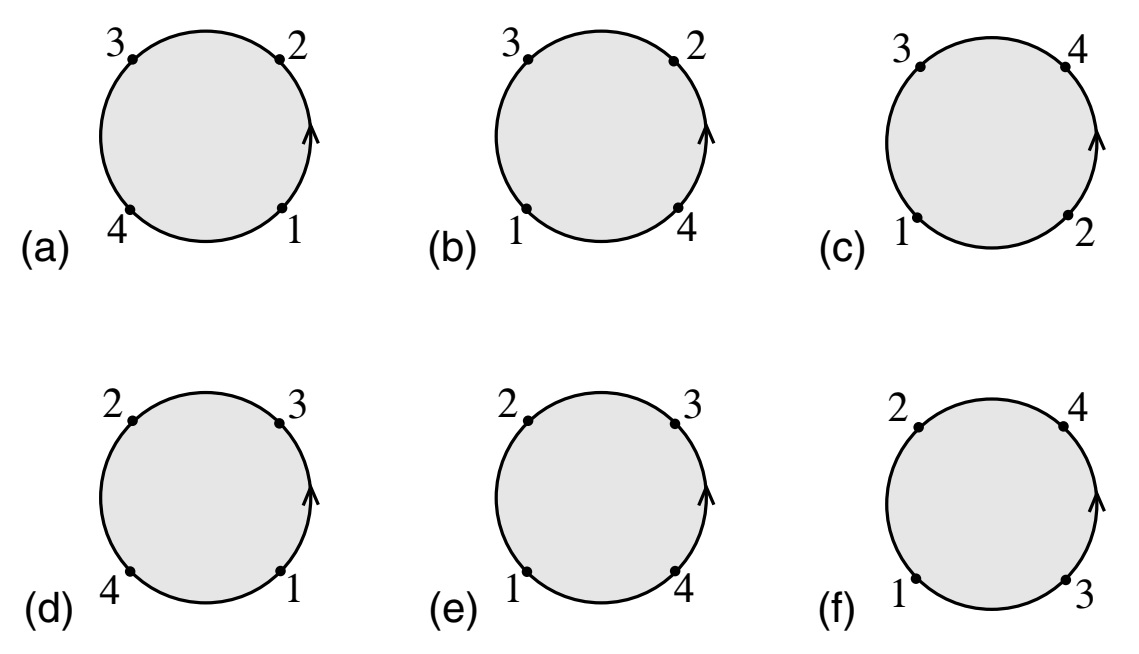
\includegraphics[width=0.5\textwidth,natwidth=854.25,natheight=490.5]{Fig6.2.jpg}\\
		\caption{圆上4个开弦顶点算符的6个循环不等价编序. 除了在点3从$\infty$跃变到$-\infty$, 坐标$y$沿着箭头方向增长.}\label{fig:6.2}
	\end{center}
\end{figure}
	

积分分裂成三部分, $-\infty<y_{4}<0$, $0<y_{4}<1$, 以及 $1<y_{4}<\infty $.  对于这三个范围, 顶点算符的排序如图\ref{fig:6.2}(a)(b)(c)所示. 
M\"{o}bius 不变性可用于将这些范围变至其他任意一个, 所以它们给出的贡献等效于顶点算符的置换.  $(t \leftrightarrow s)$ 项给出图\ref{fig:6.2}(d)(e)(f). 
合起来
\begin{equation}
	S_{D_{2}}(k_{1} ; k_{2} ; k_{3} ; k_{4})=2 \mi g_{\mathrm{o}}^{4} C_{D_{2}}(2 \pi)^{26} \delta^{26}({\textstyle\sum_{i} k_{i}})
	[I(s, t)+I(t, u)+I(u, s)] \:, \label{6.4.9}
\end{equation}
其中
\begin{equation}
	I(s, t)=\int_{0}^{1} \dif y\: y^{-\alpha^{\prime} s-2}(1-y)^{-\alpha^{\prime} t-2}  \:. \label{6.4.10}
\end{equation}
这三项分别来自于图\ref{fig:6.2}的(c)(f)、(b)(d)和(a)(e).

如果$\alpha^{\prime} s<-1$ 并且 $\alpha^{\prime} t<-1$, 积分 $I(s,t)$ 收敛. 当 $\alpha^{\prime} s \rightarrow-1$, 积分在$y=0$发散. 
为研究这一发散, 取 $y=0$ 邻域并对被积函数做近似:
	\begin{align}
		I(s, t) &=\int_{0}^{r} d y y^{-\alpha^{\prime} s-2}+\text{在$\alpha^{\prime} s=-1$处解析的项}   \nonumber \\
		&=-\frac{r^{-\alpha^{\prime} s-1}}{\alpha^{\prime} s+1}+\text{在$\alpha^{\prime} s=-1$处解析的项} \nonumber\\
		&=-\frac{1}{\alpha^{\prime} s+1}+\text{在$\alpha^{\prime} s=-1$处解析的项} \:. \label{6.4.11}
	\end{align}
在\eqref{6.4.11}中, 我们已经计算收敛区域的积分. 我们看到这一发散是$s=-1 / \alpha^{\prime}$处的极点, 开弦快子的质量平方. 
变量$s$正是散射 $1+2 \rightarrow 3+4$的质心能量平方, 所以这一极点是中间快子态所产生的共振. 再一次, 这是玻色弦的人工制品, 即最轻弦态是快子态, 与讨论无关. 
这一极点是由于图\ref{fig:6.3}(a)中的过程. 其中, 快子1和2合并变成单个快子, 然后又分离成快子3和4.

\begin{figure}[h]
	\begin{center}
		%width=0.8\textwidth,bb=0 0 1193 329
		%1px=0.75pt
		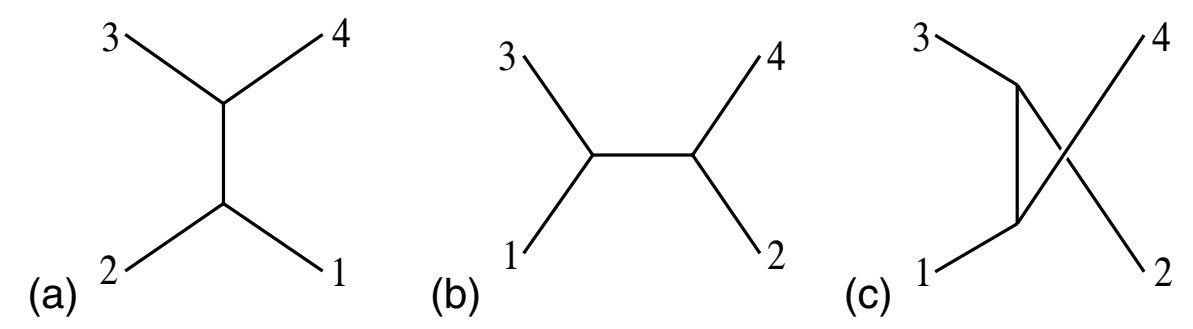
\includegraphics[width=0.5\textwidth,natwidth=894.75,natheight=246.75]{Fig6.3.jpg}\\
		\caption{在(a) $s$-, (b) $t$-, 和(c) $u$-道给出极点的过程.}\label{fig:6.3}
	\end{center}
\end{figure}

由于 $\alpha^{\prime} s=-1$ 处的奇异性只是一个极点,  可以对$I(s,t)$做解析延拓绕过这一点, 并深入到 $\alpha^{\prime} s>-1 $的区域. 
这一振幅经由解析延拓定义. 振幅在这个极点处发散是该振幅的一个显著物理特征: 中间弦态沿着长时空距离传播所对应的共振. 
绕过这一极点的发散则不是; 它仅是该振幅这一特定积分表示的人工产物. 延拓不造成任何问题. 事实上, 我们将看到每一弦发散都是这一基本形式, 
所以这种解析延拓移去了所有发散——当然, 要除去极点本身的发散. 极点在实轴上, 我们需要更精准的定义它. 对于闵可夫斯基过程, 正确的 $\epsilon$ 处理是
\begin{equation}
		\frac{1}{\alpha^{\prime} s+1}  \equiv \frac{1}{\alpha^{\prime} s+1+i \epsilon} 
		 \equiv \mathrm{P} \frac{1}{\alpha^{\prime} s+1}- \mi \pi \delta (\alpha^{\prime} s+1) \:, \label{6.4.12}
\end{equation}
其中$\mathrm{P}$ 代表主值. 幺正性(我们会在第\ref{cha:9}章系统地发展它)要求出现这一极点, 并以两个快子到一个弦的散射振幅决定了系数:
\begin{equation}
		S_{D_{2}}(k_{1} ; k_{2} ; k_{3} ; k_{4})= \mi \int \frac{\dif^{26} k}{(2 \pi)^{26}} 
		\frac{S_{D_{2}}(k_{1} ; k_{2} ; k) S_{D_{2}}(-k ; k_{3} ; k_{4})}{-k^{2}+\alpha^{\prime-1}+ \mi \epsilon} 
		+\text{ 在$k^{2}=\frac{1}{\alpha^{\prime}}$处解析的项}\:. \label{6.4.13}
\end{equation}

将4快子振幅中的因素汇聚一起, 包括$I(u, s)$对这一极点的等价贡献, 并使用3快子结果\eqref{6.4.4}, 条件\eqref{6.4.13}给出
\begin{equation}
	C_{D_{2}}=\me^{-\lambda} C_{D_{2}}^{X} C_{D_{2}}^{\mathrm{g}}=\frac{1}{\alpha^{\prime} g_{\mathrm{o}}^{2}} \:. \label{6.4.14}
\end{equation}
\begin{tcolorbox}
	\begin{remark}
		\eqref{6.4.13}给出的奇异项: 
		\[
		\mi \cdot(2 \mi g_{\mathrm{o}}^{3} C_{D_{2}})^{2}(2 \pi)^{26} \alpha^{\prime} 
		\delta^{2 b}({\textstyle\sum_{i} k_{i}}) \frac{1}{\alpha^{\prime} s+1} \:,
		\]
		\eqref{6.4.9}给出的奇异项: 
		\[
		2 \cdot 2 \mi g_{\mathrm{o}}^{4} C_{D_{2}}(2 \pi)^{26} \delta^{26}({\textstyle\sum_{i} k_{i}}) \frac{-1}{\alpha^{\prime} s+1}\:.
		\]
		二者联立给出\eqref{6.4.14}.
		\end{remark}
\end{tcolorbox}
\noindent 那么3快子振幅是
\begin{equation}
	S_{D_{2}}(k_{1} ; k_{2} ; k_{3})=\frac{2 \mi g_{\mathrm{o}}}{\alpha^{\prime}}(2 \pi)^{26} \delta^{26}({\textstyle\sum_{i} k_{i}}) \:. 
	\label{6.4.15}
\end{equation}
各种泛函行列式被扔掉了. 利用幺正性, 所有归一化可以用出现在顶点算符中的耦合 $g_{o}$ 表示. 
实际上, 行列式也可通过仔细的正规化与重整化算出, 并且不同拓扑的相对归一化与通过幺正性得出的结果一致.

解析延拓绕过极点, 我们遇到了进一步的奇异性. 在 $y=0$ 处展开被积函数
\begin{equation}
	I(s, t)=\int_{0}^{r} \dif y\: \Bigl[y^{-\alpha^{\prime} s-2}+ (\alpha^{\prime} t+2) y^{-\alpha^{\prime} s-1}+\cdots\Bigr] \:. 
	\label{6.4.16}
\end{equation}
第二项给出了$\alpha^{\prime} s=0$处的极点
\begin{equation}
	I(s, t)=\frac{u-t}{2 s}+\text{在$\alpha^{\prime} s=0$处解析的项} \:. \label{6.4.17}
\end{equation}
从泰勒展开后面的项中, 振幅的极点在
\begin{equation}
	\alpha^{\prime} s=-1,0,1,2, \ldots \:. \label{6.4.18}
\end{equation}
它们精确是开弦态的位置. 积分 $I(s, t)$ 关于变量 $t$在相同位置\eqref{6.4.18}有极点, 它们来自于端点 $y=1$.  
这是由于图\ref{fig:6.3}(b)的过程. 振幅\eqref{6.4.9}中的其他两项给出了 $s$道和 $t$ 道和$u$ 道极点(图\ref{fig:6.3}c). 
因为\eqref{6.4.17}在 $s=0$留数对 $u-t$是奇的, 这一极点实际上会与 $I(s, u)$中的极点抵消.  
$1 / \alpha^{\prime}$偶数倍处的奇点都有这样的行为. 但对于下一节要引入的更一般的开弦理论, 这不再成立.

定义欧拉 beta 函数
\begin{equation}
	B(a, b)=\int_{0}^{1} \dif y\: y^{a-1}(1-y)^{b-1} \:, \label{6.4.19}
\end{equation}
使得
\begin{equation}
	I(s, t)=B(-\alpha_{\mathrm{o}}(s),-\alpha_{\mathrm{o}}(t)), \qquad \alpha_{\mathrm{o}}(x)=1+\alpha^{\prime} x \:. 
	\label{6.4.20}
\end{equation}
这可以表达为gamma函数. 对于固定的$w$, 定义 $y=v / w$, 这给出 
\begin{equation}
	w^{a+b-1} B(a, b)=\int_{0}^{w} \dif v \: v^{a-1}(w-v)^{b-1} \:. \label{6.4.21}
\end{equation}
两边乘以$\me^{-w}$并积分 $\int_{0}^{\infty} \dif w$, 重新组合给出
\begin{align}
	\Gamma(a+b) B(a, b) &=\int_{0}^{\infty} \dif v\: v^{a-1} \me^{-v} \int_{0}^{\infty} \dif(w-v) \: (w-v)^{b-1} \me^{-(w-v)} \nonumber \\
	&=\Gamma(a) \Gamma(b) \:. \label{6.4.22}
\end{align}
那么4快子振幅就是
\begin{align}
	&S_{D_{2}}(k_{1}; k_{2} ; k_{3} ; k_{4})=\frac{2 \mi g_{\mathrm{o}}^{2}}{\alpha^{\prime}}
	(2 \pi)^{26} \delta^{26}({\textstyle \sum_{i} k_{i}}) \nonumber \\
	&\qquad \times\Bigl[B(-\alpha_{\mathrm{o}}(s),-\alpha_{\mathrm{o}}(t))+B(-\alpha_{\mathrm{o}}(s),-\alpha_{\mathrm{o}}(u))
	+B(-\alpha_{\mathrm{o}}(t),-\alpha_{\mathrm{o}}(u))\Bigr] \:, \label{6.4.23}
\end{align}
其中
\begin{equation}
	B(-\alpha_{\mathrm{o}}(x),-\alpha_{\mathrm{o}}(y))=
	\frac{\Gamma(-\alpha^{\prime} x-1) \Gamma(-\alpha^{\prime} y-1)}{\Gamma(-\alpha^{\prime} x-\alpha^{\prime} y-2)} \:. \label{6.4.24}
\end{equation}
这是Veneziano振幅, 最早是为了模拟强相互作用的某些特征而写下的.

Veneziano振幅的高能行为是重要的. 有两个感兴趣的区域, Regge极限,
\begin{equation}
	s \rightarrow \infty, \quad t \text{ 固定} \:, \label{6.4.25}
\end{equation}
以及硬散射极限
\begin{equation}
	s \rightarrow \infty, \quad t / s \text{ 固定} \:. \label{6.4.26}
\end{equation}
如果我们考虑散射过程$1+2 \rightarrow 3+4$ (使得 $k_{1}^{0}$ 和$k_{2}^{0}$ 是正的, 而 $k_{3}^{0}$ 和 $k_{4}^{0}$ 是负的), 
那么在 $1$-$2$ 质心系中,
\begin{equation}
	s=E^{2}, \quad t=(4 m^{2}-E^{2}) \sin^{2}\frac{\theta}{2}, \quad u=(4 m^{2}-E^{2}) \cos ^{2} \frac{\theta}{2} \:, \label{6.4.27}
\end{equation}
其中 $E$ 是质心系能量, 而$\theta$ 是粒子1与3之间夹角. Regge极限是高能与小角度, 而硬散射极限是高能与固定角. 利用Stirling近似, 
$\Gamma(x+1) \approx x^{x} \me^{-x}(2 \pi x)^{1 / 2}$, Regge 区域的行为是
\begin{equation}
	S_{D_{2}}(k_{1} ; k_{2} ; k_{3} ; k_{4}) \propto s^{\alpha_{\mathrm{o}}(t)} \Gamma(-\alpha_{0}(t)) \:, \label{6.4.28}
\end{equation}
其中$\alpha_{\mathrm{o}}(t)=\alpha^{\prime} t+1 $, 即振幅按照$s$的幂次变化, 而幂次依赖于$t$. 这是Regge行为. 
在gamma函数的极点振幅是$s$的整数次幂, 对应于交换整数自旋 $\alpha_{o}(t)$的弦.

在硬散射极限下
\begin{equation}
	S_{D_{2}}(k_{1} ; k_{2} ; k_{3} ; k_{4}) \approx \exp \bigl[-\alpha^{\prime}(s \ln s \alpha^{\prime}+t \ln t \alpha^{\prime}+u \ln u \alpha^{\prime})\bigr]=\exp [-\alpha^{\prime} s f(\theta)] \:, \label{6.4.29}
\end{equation}
其中
\begin{equation}
	f(\theta) \approx-\sin ^{2} \frac{\theta}{2} \ln \sin ^{2} \frac{\theta}{2}-\cos ^{2} \frac{\theta}{2} \ln \cos ^{2} \frac{\theta}{2}
	\label{6.4.30}
\end{equation}
是正的.  \eqref{6.4.29}值得注意. 高能、固定角散射探查了被散射物体的内部结构. Rutherford用硬$\alpha$原子散射发现了原子核.  
SLAC上的电子-核子硬散射揭示了核子的夸克组分. 在量子场论中, 硬散射振幅按$s $幂次衰减. 即使是像核子这样的复合物体, 如果它的组分是类点的, 它也是幂次律振幅 . 
指数衰减\eqref{6.4.29}则软的多, 体现了一个尺寸为$\alpha^{1 / 2}$的物体, 这是我们所期待的. 

我们从三点振幅开始, 跳过了零点、一点和两点振幅. 我们会在\ref{sec:6.6}节讨论这些振幅以及它们的解释 .

\section{Chan-Paton因子和规范相互作用} \label{sec:6.5}%{6.5 Chan-Paton factors and gauge interactions}

在本节我们将考察开弦无质量矢量态的相互作用. 为了使这个讨论有趣些, 我们首先来推广开弦理论.

在第\ref{cha:3}章末尾, 我们引入了一大类玻色弦理论, 但对相互作用的初步考察中, 我们集中于26维平坦时空的简单情况. 
可以用对称性的方式思考它: 这一理论有极大的26维庞加莱不变性. 在玻色闭弦中, 这是拥有这一对称性的唯一理论. 
证明的概述如下: 时空平移的世界面诺特流有权重为(1,0)和(0,1)的分量.  通过\ref{sec:2.9}节所给出的讨论, 
这些流关于$z$或$\bar{z}$是全纯的. 在本章的计算中, 这足以决定所有期望值.

然而, 在开弦理论中存在一个推广. 开弦有边界, 端点. 在含有可区分端点的量子系统中, 除了在块中传播的场外, 在这些点上很自然地含有自由度. 
在开弦的每一端点, 我们增加新的自由度, 称为Chan-Paton自由度, 它可以是 $n$ 个态中的一个. 那么弦态的基是
\begin{equation}
	|N ; k ; i j\rangle \:, \label{6.5.1}
\end{equation}
其中 $i$ 和 $j$ 标记左端点和右端点的态, 从1取到$n$. 能动量张量像往常那样定义, 对新自由度没有依赖关系. 因而, 共形不变性是自动的. 
正如Chan-Paton自由度是不变的, 庞加莱不变性也是自动的. 尽管这些新自由度的世界面动力学很平庸, 但对于时空物理, 它们有深远的影响. 

\begin{figure}[h]
	\begin{center}
		%width=0.8\textwidth,bb=0 0 529 156
		%1px=0.75pt
		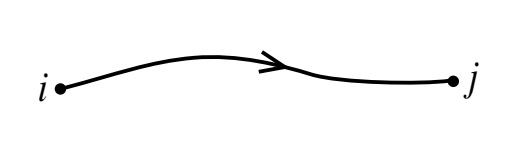
\includegraphics[width=0.5\textwidth,natwidth=396.75,natheight=117]{Fig6.4.jpg}\\
		\caption{带有Chan--Paton自由度的开弦}\label{fig:6.4}
	\end{center}
\end{figure}

在强相互作用的弦理论中, 引入Chan-Paton因子的动机是为了引入$S U(3)$ 味量子数: 端点就像夸克和反夸克, 通过色-电流管相连接. 现在我们在更广泛的框架下引入它: 考察所有可能的对称性. 在第\ref{cha:8}章, 我们将给Chan-Paton自由度一个新解释, 在第14章将附加一个可能的进一步的改进 .

现在有 $n^{2}$ 个标量快子, $n^{2}$ 个无质量矢量玻色子, 以此类推. 引入$n^{2}$个厄米矩阵$\lambda_{i j}^{a}$, 并做归一化
\begin{equation}
	\operatorname{Tr}(\lambda^{a} \lambda^{b})=\delta^{a b} \:, \label{6.5.2}
\end{equation}
这些矩阵是两个端点的态的完备基. 它们是$U(n)$的表示矩阵, 所以可以猜测无质量矢量玻色子与 $U(n)$ 对称性相联系; 一会儿我们就会看到确实是这种情况.

定义基
\begin{equation}
	|N ; k ; a\rangle=\sum_{i, j=1}^{n}|N ; k ; i j\rangle \lambda_{i j}^{a}  \:. \label{6.5.3}
\end{equation}
现在考察图 \ref{fig:6.2}(a)所示的4快子振幅, 在这个图中, 顶点算符按循环序1234排列. 因为Chan-Paton自由度没有出现在哈密顿量, 
它们的态在顶点算符之间无法演化: 快子1右端点的态必须与快子2左端点的态相同, 剩余的情况以此类推. 因此, 振幅 \ref{fig:6.2}(a) 将会包含因子
\begin{equation}
	\operatorname{Tr}(\lambda^{a_{1}} \lambda^{a_{2}} \lambda^{a_{3}} \lambda^{a_{4}}) \:, \label{6.5.4}
\end{equation}
这个因子来自于每个快子的Chan-Paton波函数的重叠. 这一规则可以推广至任意振幅: 每一顶点算符现在包含来自端点自由度波函数的 Chan-Paton 因子 $\lambda_{i j}^{a}$, 
而每一世界面的振幅要乘以沿着边界的Chan-Paton因子的迹.

3快子振幅变成
\begin{align}
	S_{D_{2}}(k_{1}, a_{1} ; k_{2}, a_{2} ; k_{3}, a_{3})= 
	 \frac{\mi g_{\mathrm{o}}}{\alpha^{\prime}}(2 \pi)^{26} \delta^{26}({\textstyle\sum_{i} k_{i}}) 
	 \operatorname{Tr}(\lambda^{a_{1}} \lambda^{a_{2}} \lambda^{a_{3}}+\lambda^{a_{1}} \lambda^{a_{3}} \lambda^{a_{2}}) \:, \label{6.5.5}
\end{align}
两个轮换序现在有了不同的Chan-Paton迹. 4快子振幅是
	\begin{align}
		&S_{D_{2}}(k_{1}, a_{1} ; k_{2}, a_{2} ; k_{3}, a_{3} ; k_{4}, a_{4})
		=\frac{\mi g_{\mathrm{o}}^{2}}{\alpha^{\prime}}(2 \pi)^{26} \delta^{26}({\textstyle \sum_{i} k_{i}}) \nonumber \\
		&\quad \times \Bigl[\operatorname{Tr}(\lambda^{a_{1}} \lambda^{a_{2}} \lambda^{a_{4}} \lambda^{a_{3}}
		+\lambda^{a_{1}} \lambda^{a_{3}} \lambda^{a_{4}} \lambda^{a_{2}}) B(-\alpha_{\mathrm{o}}(s),-\alpha_{\mathrm{o}}(t)) \nonumber  \\
		&\qquad+\operatorname{Tr}(\lambda^{a_{1}} \lambda^{a_{3}} \lambda^{a_{2}} \lambda^{a_{4}}
		+\lambda^{a_{1}} \lambda^{a_{4}} \lambda^{a_{2}} \lambda^{a_{3}}) B(-\alpha_{\mathrm{o}}(t),-\alpha_{\mathrm{o}}(u))\nonumber \\
		&\qquad+\operatorname{Tr}(\lambda^{a_{1}} \lambda^{a_{2}} \lambda^{a_{3}} \lambda^{a_{4}}
		+\lambda^{a_{1}} \lambda^{a_{4}} \lambda^{a_{3}} \lambda^{a_{2}}) 
		B(-\alpha_{\mathrm{o}}(s),-\alpha_{\mathrm{o}}(u))\Bigr] \:. \label{6.5.6}
	\end{align}
再次考察幺正性关系\eqref{6.4.13}, 在$s=-1 / \alpha^{\prime}$ 处的极点使得左边获得因子
\begin{equation}
	\frac{1}{4} \operatorname{Tr}\Bigl(\{\lambda^{a_{1}}, \lambda^{a_{2}}\} \{\lambda^{a_{3}}, \lambda^{a_{4}}\}\Bigr) \:,\label{6.5.7}
\end{equation}
而右边获得因子
\begin{equation}
	\frac{1}{4} \sum_{a} \operatorname{Tr}\Bigl(\{\lambda^{a_{1}}, \lambda^{a_{2}}\} \lambda^{a}\Bigr) 
	\operatorname{Tr}\Bigl(\{\lambda^{a_{3}}, \lambda^{a_{4}}\} \lambda^{a}\Bigr) \:, \label{6.5.8}
\end{equation}
即对中间态的Chan-Paton波函数求和.  $\lambda_{i j}^{a}$ 的完备性与归一化\eqref{6.5.2}暗示了对于任意的$A$和$B$, 有
\begin{equation}
	\operatorname{Tr}(A \lambda^{a}) \operatorname{Tr}(B \lambda^{a})=\operatorname{Tr}(A B) \:,  \label{6.5.9}
\end{equation}
因而振幅依旧是幺正的.

\begin{tcolorbox}
	\begin{proof}
		记$\operatorname{Tr}(A \lambda^{a})=\langle A \vert \lambda^{a}\rangle=\langle\lambda^{a}|A\rangle$, 那么
		\[
		\operatorname{Tr}(A \lambda^{a}) \operatorname{Tr}(B \lambda^{a}) = 
		\langle A \vert \lambda^{a}\rangle\langle\lambda^{\alpha} \vert B\rangle=\langle A \vert B\rangle \:,
		\]
		其中 $\sum_{a}|\lambda^{a}\rangle\langle\lambda^{a}|=1$ 来自于 $\langle\lambda^{a} \vert \lambda^{b}\rangle= \delta^{a b}$.
	\end{proof}	
\end{tcolorbox}



\subsection*{规范相互作用}
一个规范玻色子与两个快子的振幅是	
\begin{align}
	&S_{D_{2}}(k_{1}, a_{1}, e_{1} ; k_{2}, a_{2} ; k_{3}, a_{3})= 
	-\mi g_{\mathrm{o}}^{\prime} g_{\mathrm{o}}^{2} \me^{-\lambda} e_{1 \mu} \nonumber \\
	&\quad \times\Bigl\langle \bno c^{1} \dot{X}^{\mu} \me^{\mi k_{1} \cdot X}(y_{1})\bno 
	 \bno  c^{1} \me^{\mi k_{2} \cdot X}(y_{2})\bno \bno c^{1} \me^{\mi k_{3} \cdot X}(y_{3})\bno\Bigr\rangle_{D_{2}} 
	\operatorname{Tr}(\lambda^{a_{1}} \lambda^{a_{2}} \lambda^{a_{3}})  \nonumber\\
	&\qquad \qquad +(k_{2}, a_{2}) \leftrightarrow(k_{3}, a_{3}) \:. \label{6.5.10}
\end{align}
我们使用了玻色顶点算符\eqref{3.6.26}, 但暂且允许一个独立的归一化常数 $g_{\mathrm{o}}^{\prime}$. 利用\ref{sec:6.2}节结果,  
$X$的路径积分是
\begin{align}
	&\Bigl\langle \bno \dot{X}^{\mu} \me^{\mi k_{1} \cdot X}(y_{1})\bno \bno \me^{\mi k_{2} \cdot X}(y_{2})\bno 
	\bno \me^{\mi k_{3} \cdot X}(y_{3})\bno \Bigr\rangle_{D_{2}} 
	=-2 \mi \alpha^{\prime}\biggl(\frac{k_{2}^{\mu}}{y_{12}}+\frac{k_{3}^{\mu}}{y_{13}}\biggr) \nonumber \\
	&\qquad \times \mi C_{D_{2}}^{X}(2 \pi)^{26} \delta^{26}({\textstyle \sum_{i} k_{i}})
	|y_{12}|^{2 \alpha^{\prime} k_{1} \cdot k_{2}}|y_{13}|^{2 \alpha^{\prime} k_{1} \cdot k_{3}} 
	|y_{23}|^{2 \alpha^{\prime} k_{2} \cdot k_{3}} \:. \label{6.5.11}
\end{align}
利用动量守恒、质壳条件, 以及物理态条件$k_{1} \cdot e_{1}=0$, 振幅变成
\begin{align}
	&S_{D_{2}}(k_{1}, a_{1}, e_{1} ; k_{2}, a_{2} ; k_{3}, a_{3}) \nonumber \\
	&=-\mi g_{\mathrm{o}}^{\prime} e_{1} \cdot k_{23}(2 \pi)^{26} \delta^{26}({\textstyle \sum_{i} k_{i}}) 
	\operatorname{Tr}\Bigl(\lambda^{a_{1}}[\lambda^{a_{2}}, \lambda^{a_{3}}]\Bigr) \:, \label{6.5.12}
\end{align}
其中 $k_{i j} \equiv k_{i}-k_{j} $.  这又一次独立于顶点算符的位置.

4快子振幅中的 $s=0$ 极点不再为零. 被抵消的那一项现在有次序不同的Chan-Paton因子, 因此极点正比于
\begin{equation}
	\operatorname{Tr}\Bigl([\lambda^{a_{1}}, \lambda^{a_{2}}][\lambda^{a_{3}}, \lambda^{a_{4}}]\Bigr) \:. \label{6.5.13}
\end{equation}
通过幺正性将这一极点的系数与振幅\eqref{6.5.12}相关联, 获得
\begin{equation}
	g_{\mathrm{o}}^{\prime}=(2 \alpha^{\prime})^{-1 / 2} g_{\mathrm{o}} \:. \label{6.5.14}
\end{equation}
这与从态算符映射导出的相对归一化相同: 仅存在一个独立的耦合常数. 

对于3规范玻色子耦合, 一个类似的计算给出
\begin{align}
	&S_{D_{2}}(k_{1}, a_{1}, e_{1} ; k_{2}, a_{2}, e_{2} ; k_{3}, a_{3}, e_{3}) \nonumber \\
	&\qquad = \mi g_{\mathrm{o}}^{\prime}(2 \pi)^{26} \delta^{26}({\textstyle\sum_{i} k_{i}})
	\Bigl(e_{1} \cdot k_{23} e_{2} \cdot e_{3}+e_{2} \cdot k_{31} e_{3} \cdot e_{1}+e_{3} \cdot k_{12} e_{1} \cdot e_{2} \nonumber\\
	&\qquad \qquad +\frac{\alpha^{\prime}}{2} e_{1} \cdot k_{23} e_{2} \cdot k_{31} e_{3} \cdot k_{12} \Bigr) 
	\operatorname{Tr}\Bigl(\lambda^{a_{1}}[\lambda^{a_{2}}, \lambda^{a_{3}}]\Bigr) \:. \label{6.5.15}
\end{align}

至动量的一阶, 我们所发现的振幅可以通过如下时空作用量重新产生: 
\begin{equation}
		\bm{S}=\frac{1}{g_{\mathrm{o}}^{\prime 2}} \int \dif^{26} x\: \biggl[-\frac{1}{2} \operatorname{Tr}(D_{\mu} \varphi D^{\mu}\varphi)+\frac{1}{2 \alpha^{\prime}} \operatorname{Tr}(\varphi^{2})+\frac{2^{1 / 2}}{3 \alpha^{\prime 1 / 2}} 
		\operatorname{Tr}(\varphi^{3})
		-\frac{1}{4} \operatorname{Tr}(F_{\mu \nu} F^{\mu \nu})\biggr] \:, \label{6.5.16}
\end{equation}
其中快子场 $\varphi$ 与杨-米尔斯矢势 $A_{\mu}$ 被写成了 $n \times n$ 矩阵, 即 $A_{\mu}=A_{\mu}^{a} \lambda^{a} $. 
另外, $D_{\mu} \varphi=\partial_{\mu} \varphi-\mi[A_{\mu}, \varphi]$, 
并且 $F_{\mu \nu}=\partial_{\mu} A_{\nu}-\partial_{\nu} A_{\mu}-\mi[A_{\mu}, A_{\nu}]$.

这是$U(n)$规范场在伴随表示下与标量场相耦合的作用量. Chan-Paton因子中所增加的恰好就是规范不变表示需要的. 由于在弦微扰论中会保证非物理态的退耦, 规范不变性是自动的, 我们将会进一步研究它.

在远小于弦尺度的动量$k$处, 唯一的开弦态是无质量规范玻色子. 正如\ref{sec:3.7}节讨论的, 在这一极限下, 物理应该约化至无质量态的有效场论. 
因此, 在作用量\eqref{6.5.16}中引入快子必有某些地方不合逻辑; 我们这样做是为了启发. 但现在让我们专注于规范玻色子. 
4规范玻色子的振幅形式类似于 Veneziano 振幅, 但含有来自极化张量的额外结构. 将其展成$\alpha^{\prime} k^{2}$的幂级数, 第一项会在零斜率极限下幸存, 
它是$s, t, u$处的极点项和加上一个常数. 相容性会保证它与通过场论中的杨-米尔斯拉格朗日量$F_{\mu \nu} F^{\mu\nu} $所获得的4规范玻色子振幅精确相同. 
然而, 注意到3规范玻色子振幅\eqref{6.5.15}的$\alpha^{\prime} k^{3}$ 阶项. 这暗示了拉格朗日量中的高阶导数项
\begin{equation}
	-\frac{2 \mi \alpha^{\prime}}{3 g_{\text{o}}^{\prime 2}} \operatorname{Tr}(F_{\mu}{}^{\nu} F_{\nu}{}^{\omega} F_{\omega}{}^{\mu}) \:.
	\label{6.5.17}
\end{equation}
类似地, 展开4点振幅会揭示出高阶相互作用的无限和(除了\eqref{6.5.17}, 它们确实对3规范玻色子振幅没有运动学方面贡献). 
在低能区域, 弦的圈振幅也会约化至从有效拉格朗日量中获得的圈.  经由有效拉格朗日量的通用逻辑, 高阶导数项在低能处不是很重要, 
它们在标度 $\alpha^{\prime} k^{2} \approx 1$变得重要, 这个标度正是新物理(有质量弦态)出现的地方, 而有效作用量不再适用.

如果我们有一个截断, 为什么还需要重整化? 重整化依旧拥有内涵. 并且事实上这是它真实的解释: 它意味着, 除了有效拉格朗日量中的参量外, 低能物理与高能物理的细节无关. 
这是喜忧参半的: 它意味着我们可以在不知道普朗克标度处的理论的情况下, 利用普通的量子场论在加速器的能量级别做出预测, 
但它也意味着我们无法用粒子加速器处的物理探测普朗克能标处的理论.

弦频谱与振幅有一个显然的整体$U(n)$对称性,
\begin{equation}
	\lambda^{a} \rightarrow U \lambda^{a} U^{\dagger} \:, \label{6.5.18}
\end{equation}
它保持 Chan-Paton迹以及态的范数不变. 从振幅的细节, 我们看到这实际上时空的定域对称性. 我们将看到从整体世界面对称性到定域时空对称性的提升在弦论中是十分普遍的现象.

所有开弦态按照$U(n)$对称性下的 $n \times n$ 伴随表示变换. 顺带地, $U(n)$ 不是单李代数: $U(n)=S U(n) \times U(1) $. 
$U(1)$的规范玻色子, $\lambda_{i j}=\delta_{i j} / n^{1 / 2}$, 从振幅\eqref{6.5.12}和\eqref{6.5.15}中退耦. 
$U(1)$的伴随表示是平庸的, 所以所有弦态在$U(1)$对称下是中性的.

\subsection*{非定向弦}

推广到非定向弦是有趣的. 首先考虑没有Chan-Paton因子的理论. 除了 M\"{o}bius 不变性外, 球面或圆盘上的$X^{\mu}$CFT 在开弦的方向反射对称性 $\sigma^{1} \rightarrow \pi-\sigma^{1}$或是闭弦上的$\sigma^{1} \rightarrow 2 \pi-\sigma^{1}$下是不变的. 
世界面宇称由算符 $\Omega$ 生成. 从模式展开得出, 在开弦中
\begin{equation}
	\Omega \alpha_{n}^{\mu} \Omega^{-1}=(-1)^{n} \alpha_{n}^{\mu} \:, \label{6.5.19}
\end{equation}
在闭弦中
\begin{equation}
	\Omega \alpha_{n}^{\mu} \Omega^{-1}=\tilde{\alpha}_{n}^{\mu} \:. \label{6.5.20}
\end{equation}
这一对称性同时扩展到鬼场.但为了集中注意力, 我们这里不讨论它们, 它们对树图的贡献也仅仅是个固定的因子. 

无论开弦还是闭弦, 快子顶点算符在世界面宇称下是偶的 (这对于无鬼的被积顶点算符是显然的; 那么固定的算符也必须以同样的方式变换), 这决定了算符的符号. 
那么所有的态可以根据它们的宇称本征值 $\omega=\pm 1 $分类.  开弦中的关系\eqref{6.5.19}暗示了
\begin{equation}
	\Omega|N ; k\rangle=\omega_{N}|N ; k\rangle, \quad \omega_{N}=(-1)^{1+\alpha^{\prime} m^{2}} \:. \label{6.5.21}
\end{equation}
世界面宇称是乘积守恒. 例如, 3快子振幅非零, 与 $(+1)^{3}=1$ 相容.  另一方面, 无质量矢量有 $\omega=-1$, 所以我们可以预期在没有Chan-Paton因子时, 
矢量-快子-快子振幅\eqref{6.5.10}与3矢量振幅\eqref{6.5.15}为零, 结果也确实如此 ($\lambda^{a}$ 被替换成1, 而对易子为零). 
不同的轮换顺序, 也通过世界面宇称彼此相关, 因而相互抵消.

给定一个相容的定向弦论, 通过将频谱限制在$\omega=+1$的态上, 我们给出了新的非定向弦论.  $\alpha^{\prime} m^{2}$ 为奇的态保留, 
而 $\alpha^{\prime} m^{2}$为偶的态, 包括光子, 被禁止了. $\omega$ 守恒保证了, 如果所有的外态有$\omega=+1$, 那么树图的中间态也有 $\omega=+1$. 
因此, 至少在树图级, 非定向弦的幺正性从定向弦的幺正性得出. 

对于非定向理论的主要兴趣就在于Chan-Paton因子的处理. 由于我们能识别出开弦的相对端点, 世界面宇称必会反转它们
\begin{equation}
	\Omega|N ; k ; i j\rangle=\omega_{N}|N ; k ; j i\rangle \:. \label{6.5.22}
\end{equation}
再一次, 这是定向理论中所有振幅的一个对称性. 为了构成非定向理论, 我们再一次将频谱约束到世界面宇称本征值 $\omega=+1 $. 
取 $\lambda_{i j}^{a}$ 的一组基, 使得每个矩阵要么对称 $s^{a}=+1$;要么反对称,  $s^{a}=-1$. 那么
\begin{equation}
	\Omega|N ; k ; a\rangle=\omega_{N} s^{a}|N ; k ; a\rangle \:. \label{6.5.23}
\end{equation}
世界面宇称本征值是 $\omega=\omega_{N} s^{a}$, 那么非定向频谱是
\begin{subequations} \label{6.5.24}
\begin{align}
&\text{偶数倍的}\alpha^{\prime} m^{2} \:: \qquad   \text{反对称的 } \lambda^{a}  \:, \label{6.5.24a} \\ 	
&\text{奇数倍的}\alpha^{\prime} m^{2} \:: \qquad   \text{\phantom{反}对称的 } \lambda^{a}  \:. \label{6.5.24b} 
\end{align}			
\end{subequations}
对于无质量规范玻色子, Chan-Paton因子是 $n \times n$ 反对称矩阵, 所以规范群是 $S O(n) $.  偶数质量能级的态按照正交群 $S O(n)$的伴随表示变换, 而奇数质量能级的态按照无迹对称张量加一个单态表示变换.

定向理论有一大类方向反演对称性, 它们作为 $\Omega$ 与 $U(n)$ 旋转的组合获得
\begin{equation}
	\Omega_{\gamma}|N ; k ; i j\rangle=\omega_{N} \gamma_{j j^{\prime}}\left|N ; k ; j^{\prime} i^{\prime}\right\rangle \gamma_{i^{\prime} i}^{-1} \:. \label{6.5.25}
\end{equation}
通过将频谱约束至 $\omega_{y}=+1$,我们可以构造更加普遍的非定向理论. 这又一次与相互作用是相容的, 用 $\Omega_{\gamma}$ 作用两次给出
\begin{equation}
	\Omega_{\gamma}^{2}|N ; k ; i j\rangle= [(\gamma^{T})^{-1} \gamma]_{i i^{\prime}}
	|N ; k ; i^{\prime} j^{\prime}\rangle (\gamma^{-1} \gamma^{T})_{j^{\prime} j} \:. \label{6.5.26}
\end{equation}
我们假定 $\Omega_{\gamma}^{2}=1$ , 原因会在下面解释. 这暗示了
\begin{equation}
	\gamma^{T}=\pm \gamma \:. \label{6.5.27}
\end{equation}
即, $\gamma$是对称或反对称的.

Chan-Paton的基变换是
\begin{equation}
	|N ; k ; i j\rangle^{\prime}=U_{i i^{\prime}}^{-1} |N ; k ; i^{\prime} j^{\prime}\rangle U_{j^{\prime} j} \:, \label{6.5.28}
\end{equation}
这将 $\gamma$变到
\begin{equation}
	\gamma^{\prime}=U^{T} \gamma U \:. \label{6.5.29}
\end{equation}
在对称情形下, 总能找到一组基, 使得 $\gamma=1$, 这给出上面已经考察过的情况. 在反对称的情况下, 存在一组基, 使得
\begin{equation}
	\gamma=M \equiv \mi\begin{bmatrix}
		0 & I \\
		-I & 0
	\end{bmatrix} \:. \label{6.5.30}
\end{equation}
这里 $I$ 是 $k \times k$ 单位矩阵, 由于  $\gamma$是可逆反对称矩阵, $n=2 k$ 必须为偶. 我们取Chan-Paton 波函数的一组基, 
使得 $M(\lambda^{a})^{T} M=s^{a^{\prime}} \lambda^{a}$, 其中 $s^{a^{\prime}}=\pm 1$. 
那么世界面本征值是 $\omega_{\gamma}=\omega_{N} s^{a^{\prime}}$, 并且非定向频谱是
\begin{subequations} \label{6.5.31}
\begin{align}
\text{偶数倍的 }\alpha^{\prime} m^{2} \:: \qquad   M(\lambda^{a})^{T} M=-\lambda^{a} \:, \label{6.5.31a} \\
\text{奇数倍的 }\alpha^{\prime} m^{2} \:: \qquad   M(\lambda^{a})^{T} M=+\lambda^{a} \:. \label{6.5.31b}
\end{align}
\end{subequations}
在偶数质量能级, 包括规范玻色子, 这定义了辛群 $S p(k)$ 的伴随表示.

为了构建非定向理论, 我们必须有 $\Omega_{\gamma}^{2}=1$, 理由如下. 既然$\Omega^{2}=1$, 
$\Omega_{\gamma}^{2}$必须仅作用于Chan-Paton因子上. 事实上, 从\eqref{6.5.26}, 它在 Chan-Paton 波函数上的作用为
\begin{equation}
	\lambda \rightarrow (\gamma^{T})^{-1} \gamma \lambda \gamma^{-1} \gamma^{T}=\lambda \:, \label{6.5.32}
\end{equation}
其中, 由于所有的态在$\Omega_{\gamma}$ 下是不变的, 最后一个等号在非定向理论中必须成立. 现在我们断言所允许的 Chan-Paton 波函数必构成完备基. 
关键在于, 两个开弦通过图\ref{fig:3.4}(c)的分裂聚合相互作用可以交换端点. 以这种方式, 可以到达一个完备基, 即到达任一个Chan-Paton 态$|i j\rangle$. 通过 Schur引理, 如果\eqref{6.5.32}对完备基成立, 那么 $\gamma^{-1} \gamma^{T}=1$ , 因而 $\Omega_{\gamma}^{2}=1$.

通过取 $\lambda^{a} $ 的不同集合, 我们可以试图获得不同的规范理论. 事实上, 上面构建的定向 $U(n)$ 理论与非定向的$S O(n)$和 $S p(k)$ 理论是唯一的可能性. 
\eqref{6.5.7} -- \eqref{6.5.9}中完备性讨论的推广表明它们是非定向理论的最一般解. 特别地, 例外李代数无法从Chan-Paton因子获得. 
在闭弦理论中, 有其他机制给出规范玻色子, 并且允许其他群.

\section{闭弦树图振幅} \label{sec:6.6}%{6.6 Closed string tree amplitudes}

关于闭弦振幅的讨论与上面类似. 3闭弦快子的振幅是
\begin{equation}
	S_{S_{2}}(k_{1} ; k_{2} ; k_{3})=g_{\mathrm{c}}^{3} \me^{-2 \lambda}\left\langle\prod_{i=1}^{3} 
	: \mathrel{\tilde{c} c \me^{\mi k_{i} \cdot X}(z_{i}, \bar{z}_{i})}:\right\rangle \bigg._{\!\!S_{2}} \:. \label{6.6.1}
\end{equation}
在这一情况下, CKG $PSL(2, \mathds{C})$ (M\"{o}bius群) 可以将三个顶点算符固定在任意位置 $z_{1,2,3}$. 从\ref{sec:6.2}节中取期望值, 
结果又一次独立于顶点算符,
\begin{equation}
	S_{S_{2}}(k_{1} ; k_{2} ; k_{3})= \mi g_{\mathrm{c}}^{3} C_{S_{2}}(2 \pi)^{26} \delta^{26}({\textstyle \sum_{i} k_{i}}) \:, 
	\label{6.6.2}
\end{equation}
其中 $C_{S_{2}}=\me^{-2 \lambda} C_{S_{2}}^{X} C_{S_{2}}^{\mathrm{g}}$.

对于4闭弦快子
\begin{equation}
	S_{S_{2}}(k_{1} ; k_{2} ; k_{3} ; k_{4})=g_{\mathrm{c}}^{4} \me^{-2 \lambda} 
	\int_{\mathds{C}} \dif^{2} z_{4} \: \left\langle\prod_{i=1}^{3}
	: \mathrel{\tilde{c} c \me^{\mi k_{i} \cdot X}(z_{i}, \bar{z}_{i})}:
	: \mathrel{\me^{\mi k_{4} \cdot X}(z_{4}, \bar{z}_{4})}:\right\rangle\bigg._{\!\!S_{2}} \:, \label{6.6.3}
\end{equation}
其中积分范围为整个复平面$\mathds{C}$. 计算期望值并令 $z_{1}=0, z_{2}=1, z_{3}=\infty$, 这变成
\begin{equation}
	S_{S_{2}}(k_{1} ; k_{2} ; k_{3} ; k_{4}) = 
	\mi g_{\mathrm{c}}^{4} C_{S_{2}}(2 \pi)^{26} \delta^{26}({\textstyle\sum_{i} k_{i}}) J(s, t, u) \:, \label{6.6.4}
\end{equation}
其中
\begin{equation}
	J(s, t, u)=\int_{\mathds{C}} \dif^{2} z_{4}\: |z_{4}|^{-\alpha^{\prime} u / 2-4}|1-z_{4}|^{-\alpha^{\prime} t/2-4}\:. \label{6.6.5}
\end{equation}
这里 $s+t+u=-16 / \alpha^{\prime}$, 我们这里标记出了$J$对所有3个变量的相关性, 这是为了强调它们之间的对称性. 
当$s, t, u<-4 / \alpha^{\prime}$, 振幅收敛. 当 $z_{4} \rightarrow 0$, 它有关于$u$的极点;当 $z_{4} \rightarrow 1$, 它有关于$t$的极点; 
当 $z_{4} \rightarrow \infty$, 它有关于$s$的极点. 这些极点所处位置: 
\begin{equation}
	\alpha^{\prime} s\,,\: \alpha^{\prime} t \,,\: \alpha^{\prime} u=-4,0,4,8, \ldots,\label{6.6.6}
\end{equation}
它们是闭弦态的质量平方. $\alpha^{\prime} s=-4$ 处的极点是
\begin{equation}
	\mi g_{\mathrm{c}}^{4} C_{S_{2}} \int_{|z_{4}|>1 / \epsilon} \dif^{2} z_{4}\: |z_{4}|^{\alpha^{\prime} s / 2} 
	\sim-\frac{8 \pi \mi g_{\mathrm{c}}^{4} C_{S_{2}}}{\alpha^{\prime} s+4} \:. \label{6.6.7}
\end{equation}
幺正性给出
\begin{equation}
	C_{S_{2}}=\frac{8 \pi}{\alpha^{\prime} g_{\mathrm{c}}^{2}} \:, \label{6.6.8}
\end{equation}
因此
\begin{equation}
	S_{S_{2}}(k_{1} ; k_{2} ; k_{3})=\frac{8 \pi \mi g_{\mathrm{c}}}{\alpha^{\prime}}(2 \pi)^{26} 
	\delta^{26}({\textstyle\sum_{i} k_{i}}) \:. \label{6.6.9}
\end{equation}

类似于Veneziano振幅, 4闭弦快子振幅可以表述成gamma 函数:
\begin{equation}
	S_{S_{2}}(k_{1} ; k_{2} ; k_{3} ; k_{4})=\frac{8 \pi \mi g_{\mathrm{c}}^{2}}{\alpha^{\prime}}(2 \pi)^{26} 
	\delta^{26}({\textstyle \sum_{i} k_{i}}) C(-\alpha_{\mathrm{c}}(t),-\alpha_{\mathrm{c}}(u)) \:, \label{6.6.10}
\end{equation}
其中 $\alpha_{\mathrm{c}}(x)=1+\alpha^{\prime} x / 4$ 并且
\begin{align}
	C(a, b) &=\int_{\mathds{C}} \dif^{2} z \: |z|^{2 a-2}|1-z|^{2 b-2} \nonumber \\
	&=2 \pi \frac{\Gamma(a) \Gamma(b) \Gamma(c)}{\Gamma(a+b) \Gamma(a+c) \Gamma(b+c)}\:, \quad a+b+c=1 \:. \label{6.6.11}
\end{align}
这是 Virasoro-Shapiro 振幅. 这里只有一项, 并且 $s, t, u$道中的极点来自于分子中的gamma函数. 类似于Veneziano 振幅,  Virasoro-Shapiro 振幅在 Regge极限下有Regge 行为
\begin{equation}
	S_{S_{2}}(k_{1} ; k_{2} ; k_{3} ; k_{4}) \propto s^{2 \alpha_{\mathrm{c}}(t)} 
	\frac{\Gamma(-\alpha_{\mathrm{c}}(t))}{\Gamma(1+\alpha_{\mathrm{c}}(t))} \:, \label{6.6.12}
\end{equation}
并且在硬散射极限下有指数行为
\begin{equation}
	S_{S_{2}}(k_{1} ; k_{2} ; k_{3} ; k_{4}) \propto \exp 
	\biggl[-\frac{\alpha^{\prime}}{2}(s \ln s \alpha^{\prime}+t \ln t \alpha^{\prime}+u \ln u \alpha^{\prime})\biggr] \:. \label{6.6.13}
\end{equation}

在球面上, 一个无质量闭弦和两个闭弦快子的振幅是
\begin{align}
		S_{S_{2}}(k_{1}, e_{1} ; k_{2} ; k_{3}) &= g_{\mathrm{c}}^{2} g_{\mathrm{c}}^{\prime} 
		\me^{-2 \lambda} e_{1 \mu \nu} \Biggl\langle: \mathrel{\tilde{c} c \partial X^{\mu} \bar{\partial} X^{\nu} 
		\me^{\mi k_{1} \cdot X}(z_{1}, \bar{z}_{1})}: \nonumber \\
		&\qquad \qquad \quad : \mathrel{\tilde{c} c \me^{\mi k_{2} \cdot X}(z_{2}, \bar{z}_{2})}:
		: \mathrel{\tilde{c} c \me^{\mi k_{3} \cdot X}(z_{3}, \bar{z}_{3})}: \biggr\rangle_{S_{2}}  \nonumber \\
		& =-\frac{\pi \mi \alpha^{\prime}}{2} g_{\mathrm{c}}^{\prime} e_{1 \mu \nu} k_{23}^{\mu} k_{23}^{\nu}
		(2 \pi)^{26} \delta^{26}({\textstyle\sum_{i} k_{i}}) \:, \label{6.6.14}
\end{align}
其中 $e_{1 \mu \nu} e_{1}^{\mu \nu}=1$. 在$s=0$极点处展开Virasoro-Shapiro振幅\eqref{6.6.10}, 利用幺正性可以给出
\begin{equation}
	g_{\mathrm{c}}^{\prime}=\frac{2}{\alpha^{\prime}} g_{\mathrm{c}} \:, \label{6.6.15}
\end{equation}
这又一次与含有总常数 $g_{\mathrm{c}} $的态-算符对应一致.  振幅\eqref{6.6.14}可以通过作用量 $\bm{S}+\bm{S}_{T}$从场论中获得, 
其中 $\bm{S}$ 是无质量场的作用量\eqref{3.7.20}, 而
\begin{equation}
	\bm{S}_{T}=-\frac{1}{2} \int \dif^{26} x\: (-G)^{1 / 2} \me^{-2 \tilde{\Phi}}
	\biggl(G^{\mu \nu} \partial_{\mu} T \partial_{\nu} T-\frac{4}{\alpha^{\prime}} T^{2} \biggr) \:, \label{6.6.16}
\end{equation}
这是闭弦快子$T$的作用量. 例如, 极化为 $e_{\mu \nu}$ 的引力子振幅可以通过展开
\begin{equation}
	\tilde{G}_{\mu \nu}=\eta_{\mu \nu}-2 \kappa e_{\mu \nu} \me^{\mi k \cdot x} \:, \label{6.6.17}
\end{equation}
从这一作用量获得. 注意到这是爱因斯坦度规, 它的作用量\eqref{3.7.25}中不含伸缩子. 涨落的归一化由时空作用量中引力子动能项的涨落决定. 
特别地, 如果取 $\tilde{G}_{\mu \nu}-\eta_{\mu \nu}=-2 \kappa e_{\mu \nu} f(x)$ 其中$e_{\mu \nu} e^{\mu \nu}=1$, 
$f$的有效作用量有实标量的正则归一化 $\frac{1}{2}$. 场论振幅与弦论结果\eqref{6.6.14}相匹配, 并与引力耦合顶点算符的归一化相关
\begin{equation}
	\kappa=\pi \alpha^{\prime} g_{\mathrm{c}}^{\prime}=2 \pi g_{\mathrm{c}} \:. \label{6.6.18}
\end{equation}

3无质量闭弦振幅是
\begin{equation}
	S_{S_{2}}(k_{1}, e_{1} ; k_{2}, e_{2} ; k_{3}, e_{3})=\frac{\mi \kappa}{2}(2 \pi)^{26} 
	\delta^{26}(\textstyle{\sum_{i} k_{i}}) e_{1 \mu \nu} e_{2 \alpha \beta} e_{3 \gamma \delta} T^{\mu \alpha \gamma} T^{\nu \beta \delta} \:, \label{6.6.19}
\end{equation}
其中
\begin{equation}
	T^{\mu \alpha \gamma}=k_{23}^{\mu} \eta^{\alpha \gamma}+k_{31}^{\alpha} \eta^{\gamma \mu}+k_{12}^{\gamma} \eta^{\mu \alpha}+\frac{\alpha^{\prime}}{8} k_{23}^{\mu} k_{31}^{\alpha} k_{12}^{\gamma} \:. \label{6.6.20}
\end{equation}
这一振幅的$k^{2}$ 项对应时空作用量\eqref{3.7.25}, 而$k^{4}$和$k^{6}$项来自于几个高阶导数相互作用, 包括时空曲率的2次项和3次项. 
通过计算世界面$\beta$函数\eqref{3.7.14}的高圈修正也可获得作用量的高阶修正.

如果我们令开弦中$\alpha^{\prime}=\frac{1}{2}$, 闭弦中$\alpha^{\prime}=2$, 那么闭弦振幅\eqref{6.6.19}的张量结构就是开弦振幅\eqref{6.5.15}的两个复本. 
对于振幅\eqref{6.6.14}也有同样的结果. 这是球面上的自由场期望值因式分解成全纯部分和反全纯部分的结果. 在对顶点算符的位置积分前, 对于4个或多个闭弦会有类似的因子化. 
更进一步, 通过对积分围道的小心处理, 有可能发现被积振幅之间的关系. 对于4快子振幅, 在使用$\Gamma(x) \Gamma(1-x) \sin (\pi x)=\pi $之后, 
之上的积分有如下关系
\begin{equation}
	J(s, t, u, \alpha^{\prime})=-2 \sin \pi \alpha_{\mathrm{c}}(t) I(s, t, 4 \alpha^{\prime}) I(t, u, 4 \alpha^{\prime}) \:;
	\label{6.6.21}
\end{equation}
我们现在标明了积分对于 $\alpha^{\prime} $的显式相关性. 对于出现在4点闭弦振幅中的一般积分有如下关系
\begin{align}
	&\int_{\mathds{C}} \dif^{2} z\: z^{a-1+m_{1}} \bar{z}^{a-1+n_{1}}(1-z)^{b-1+m_{2}}(1-\bar{z})^{b-1+n_{2}} \nonumber \\
	&\qquad =2 \sin [\pi(b+n_{2})] B(a+m_{1}, b+m_{2}) B(b+n_{2}, 1-a-b-n_{1}-n_{2}) \:. \label{6.6.22}
\end{align}
这暗示了4点开弦振幅与4点闭弦振幅之间的关系
\begin{equation}
	A_{\mathrm{c}}(s, t, u, \alpha^{\prime}, g_{\mathrm{c}}) = 
	\frac{\pi \mi g_{\mathrm{c}}^{2} \alpha^{\prime}}{g_{\mathrm{o}}^{4}} 
	\sin [\pi \alpha_{\mathrm{c}}(t)] A_{\mathrm{o}}(s, t, \tfrac{1}{4} \alpha^{\prime}, g_{\mathrm{o}}) 
	A_{\mathrm{o}}(t, u, \tfrac{1}{4} \alpha^{\prime}, g_{\mathrm{o}})^{*} \:, \label{6.6.23}
\end{equation}
其中开弦振幅仅包含6个轮换中的一个, 而极点就在写明的道中.

\subsection*{相容性}
在第\ref{cha:9}章, 我们将以一种普遍的方式讨论树图振幅的收敛性与规范不变性, 但作为一个导引, 我们现在先用 OPE 来看一下这在最低阶是如何运作的. 考察算符乘积
\begin{align}
	&: \mathrel{\me^{\mi k_{1} \cdot X(z_{1}, \bar{z}_{1})}}: 
	: \mathrel{\me^{\mi k_{4} \cdot X(z_{4}, \bar{z}_{4})}}: = 
	|z_{14}|^{\alpha^{\prime} k_{1} \cdot k_{4}}:\!\!
	\Bigl(1+ \mi z_{14} k_{1} \cdot \partial X + \mi \bar{z}_{14} k_{1} \cdot \bar{\partial} X \nonumber \\
	&\qquad \qquad -z_{14} \bar{z}_{14} k_{1} \cdot \partial X k_{1} \cdot \bar{\partial} X+\cdots \Bigr) 
	\,\me^{\mi(k_{1}+k_{4}) \cdot X}(z_{4}, \bar{z}_{4})\!\!: \:. \label{6.6.24}
\end{align}
它出现在 $z_{14}$ 要被积掉的振幅中. 当 
\begin{equation}
	\alpha^{\prime} k_{1} \cdot k_{4}=\frac{\alpha^{\prime}}{2}(k_{1}+k_{4})^{2}-4>-2 \:, \label{6.6.25}
\end{equation}
积分在$z_{14} \rightarrow 0$ 处收敛, 并且它在${-}2$这一点有极点. 这一极点的系数就是快子顶点算符. 因此, 在任意的振幅中, 
如果一对快子有总动量 $(k_{1}+k_{4})^{2}=4 / \alpha^{\prime}$, 那么就会有一极点, 幺正性要求这个极点正比于少了一个快子的振幅. 
动量空间中的极点对应于时空中的长距离, 所以这是两个快子散射到一个快子的过程, 而这一快子又与其他粒子相互作用. 进一步做 OPE, 
$O(z_{14})$ 与$O(\bar{z}_{14})$ 项不产生快子, 这是因为角积分给出零留数, $O(z_{14} \bar{z}_{14})$给出无质量极点, 以此类推.

现在我们更细致的研究下定域时空对称性是如何在弦振幅中维持的. 如果任何一个极化矢量是如下形式 $e_{\mu}=k_{\mu}$, 
或 $e_{\mu \nu}=\zeta_{\mu} k_{\nu}+k_{\mu} \tilde{\zeta}_{\mu}$, 其中 $k \cdot \zeta=k \cdot \tilde{\zeta}=0 $, 
那么我们所计算的散射振幅均为零. 这对应于作用量在杨-米尔斯, 坐标, 以及反对称张量对称性是不变的. 正如在\ref{sec:3.6}节讨论的, 
纵向极化的顶点算符是全导数与另一项的和, 而这一项由于运动方程为零. 积分后, 全导数项为零, 但是运动方程项可能会在路径积分中的其他顶点处有源. 
当 $k_{1} \cdot k_{4}$ 很大时, 算符乘积\eqref{6.6.24}骤减为零. 利用这一性质, 对于任何一对算符, 总会有一运动学区域, 
使得其中所有可能的连通项(contact)都被压低了. 那么零(null)极化的振幅在这一区域恒为零, 因为所有振幅除了在极点外都是解析的, 零极化的振幅必须处处为零. 
我们看到由幺正性以及所有可能的发散和时空规范不变性的破坏所要求的极点,  它们产生于极限 $z \rightarrow 0,1, \infty$以及两个顶点算符靠近时. 
对于有4个标记点的球面, 它们是模空间的边界. 由于历史的原因, 这里的解析延拓讨论被称为canceled propagator argument.

\subsection*{$D_{2}$ 和 $R P_{2}$上的闭弦}
最低阶的闭弦-开弦相互作用来自于既有闭弦顶点算符又有开弦顶点算符的圆盘. 它们的低能有效作用量可以从一般讨论中推导出来. 
在一个平庸的闭弦背景下, 我们会发现通常的规范动能项,
\begin{equation}
	-\frac{1}{4 g_{\mathrm{o}}^{\prime 2}} \int \dif^{26} x\: \operatorname{Tr}(F_{\mu \nu} F^{\mu \nu}) \:. \label{6.6.26}
\end{equation}
显然度规必须与其以协变的方式耦合. 另外, 与伸缩子的耦合也可以推导出来. 回忆 $g_{\mathrm{o}}^{\prime 2} \propto \me^{\Phi_{0}}$,  
其中$\Phi_{0}$是伸缩子的期望值. 所以我们要再将其(在积分内部)替换成 $\Phi=\Phi_{0}+\tilde{\Phi}$. 作用量
\begin{equation}
	-\frac{1}{4 g_{\mathrm{o}}^{\prime 2}} \int \dif^{26} x \: (-G)^{1/2} \me^{-\tilde{\Phi}} 
	\operatorname{Tr}(F_{\mu \nu} F^{\mu \nu}) \label{6.6.27}
\end{equation}
除了闭弦场的导数外, 包含所有的相互作用; 指标现在用 $G_{\mu \nu} $升降. 这一作用量反映了: 来自欧拉数$\chi$的有效作用量含有权重$g_{\mathrm{c}}^{-\chi} \propto \me^{-\chi \Phi}$这一性质.

圆盘与射影平面对纯闭弦相互作用也有贡献. $n$个闭弦的振幅是 $g_{\mathrm{o}}^{-2} g_{\mathrm{c}}^{n} \sim g_{\mathrm{c}}^{n-1}$阶的, 
比球面要多一个$g_{\mathrm{c}}$. 对于下一节要考虑的闭弦圈振幅, 因为发射或吸收一个闭弦要增加2个$g_{\mathrm{c}} $因子, 它是 $g_{\mathrm{c}}^{2}$ 乘以球面. 
因此球面与射影平面是``半圈阶''的.

球面和射影平面上的振幅中最有趣的一种是含有单个闭弦顶点算符的振幅. 固定顶点算符的位置仅移除了三个CKV中的两个, 残余的规范变换由关于顶点算符位置的旋转构成. 
因此, 必须要给散射振幅除以残余CKG的体积. 我们还没有明晰地证明它, 但在下一章的环面将会解决这一问题. 对于有一个闭弦的圆盘, 这是一个有限且不为零的因子. 
该振幅是一个数值因子乘以 $g_{\mathrm{c}} g_{\mathrm{o}}^{-2}$,这是一纯数, 再乘以 $\alpha^{\prime}$ 的幂次(由量纲分析). 
我们在这里不会解出这些数值因子, 但在第\ref{cha:8}章会以间接的方式获得它们. 

因此, 无论从圆盘还是射影平面(动量为零), 对于从真空中出现的闭弦, 都有一个振幅, 这种振幅被称为蝌蚪振幅. 换句话说, 背景闭弦场会被它们的初始值修正到$g_{\mathrm{c}}$阶. 我们同样可以写下有效作用量
\begin{equation}
	-\Lambda \int \dif^{26} x \: (-G)^{1/2} \me^{-\tilde{\Phi}} \:, \label{6.6.28}
\end{equation}
这是伸缩子的势, 我们会在下一章进一步考察.

另一方面, 对于球面上的单个闭弦, 振幅为零, 残余的CKG是$PSL(2, \mathds{C})$ 的非紧致子群, 因而这一振幅会除以一个无限大的体积. 
非零的结果会有逻辑上的不自洽性, 即对背景场的零阶修正. 类似地, 球面上的两个闭弦振幅 (对质量的零阶修正) 也为零, 对于对应的圆盘振幅, 有一个或两个开弦时, 也为零. 
没有顶点算符的振幅也是有意义的——它们恰好计算作用量\eqref{6.6.28}的泰勒展开中$\tilde{\Phi}^{0}$ 阶项. 
没有顶点算符的圆盘因此并不为零, 这要求对共形基灵体积进行某种形式上的处理.

\section{一般结果}  \label{sec:6.7}%{6.7 General results} 

在本节, 我们将会获得关于球面和圆盘上的CFT的一些一般结果.

\subsection*{M\"{o}bius 不变性}
我们已经看到球面上有一个整体定义的共形变换群 Möbius 群 $PSL(2, \mathds{C})$
\begin{equation}
	z^{\prime}=\frac{\alpha z+\beta}{\gamma z+\delta} \:, \label{6.7.1}
\end{equation}
其中 $\alpha, \beta, \gamma, \delta$ 是复数且满足 $\alpha \delta-\beta \gamma=1$. 这是球面 $S_{2}$上最一般的一对一共形变换. 
期望值必须在任意的M\"{o}bius变换下不变:
\begin{equation}
	\bigl\langle\mathscr{A}_{i}(z_{1}, \bar{z}_{1}) \ldots \mathscr{A}_{k}(z_{n}, \bar{z}_{n})\bigr\rangle_{S_{2}} =
	\bigl\langle\mathscr{A}_{i}^{\prime}(z_{1}, \bar{z}_{1}) \ldots \mathscr{A}_{k}^{\prime}(z_{n}, \bar{z}_{n})\bigr\rangle_{S_{2}} \:. 
	\label{6.7.2}
\end{equation}
我们将考察这一对称性对于1, 2, 3, 4个定域算符的结果.

对于单个权重为 $\left(h_{i}, \tilde{h}_{i}\right)$的算符, 重新标度加上旋转 $z^{\prime}=\gamma z$ 给出
\begin{equation}
	\bigl\langle\mathscr{A}_{i}(0,0)\bigr\rangle_{S_{2}} = \bigl\langle\mathscr{A}_{i}^{\prime}(0,0)\bigr\rangle_{S_{2}}
	=\gamma^{-h_{i}} \bar{\gamma}^{-\tilde{h}_{i}}\bigl\langle\mathscr{A}_{i}(0,0)\bigr\rangle_{S_{2}} \:. \label{6.7.3}
\end{equation}
因此, 除非 $h_{i}=\tilde{h}_{i}=0$, 否则一点函数为零. 因为物质因子是$(1,1)$算符的期望值, 这是看到一点振幅在球面上为零的另一种方法.

当$n=2$, 我们可以用平移加 $z^{\prime}=\gamma z$ 可以将任何一对算符挪到位置0和1, 给出
\begin{equation}
	\bigl\langle\mathscr{A}_{i}(z_{1}, \bar{z}_{1}) \mathscr{A}_{j}(z_{2}, \bar{z}_{2})\bigr\rangle_{S_{2}}
	=z_{12}^{-h_{i}-h_{j}} \bar{z}_{12}^{-\tilde{h}_{i}-\tilde{h}_{j}}
	\bigl\langle\mathscr{A}_{i}(1,1) \mathscr{A}_{j}(0,0)\bigr\rangle_{S_{2}} \:, \label{6.7.4}
\end{equation}
所以位置相关性被完全决定了. 单值性暗示了 $J_{i}+J_{j} \in \mathds{Z}$, 其中 $J_{i}=h_{i}-\tilde{h}_{i} $.
\begin{tcolorbox}
	\begin{remark}
		$J_{i}+J_{j}=(h_{i}+h_{j})-(\tilde{h}_{i}+\tilde{h}_{j})$, 所以$z_{12} \rightarrow \me^{\mi \theta} z_{12}$, $\bar{z}_{12}\rightarrow \me^{-\mi \theta} \bar{z}_{12}$\:.
	\end{remark}
\end{tcolorbox}
\noindent 共形变换 $z^{\prime}=z+\epsilon(z-z_{1})(z-z_{2})+O(\epsilon^{2})$对两点函数有进一步的约束, 它使得 $z_{1}$ 和 $z_{2}$ 固定了. 
对于一般算符这是复杂的, 但是对于张量场 $\mathcal{O}_{p}$ 和 $\mathcal{O}_{q}$, 这就暗示了
\begin{equation}
	\text{除非}\:\: h_{p}=h_{q}, \quad \tilde{h}_{p}=\tilde{h}_{q}\:, \qquad 
	\bigl\langle\mathcal{O}_{p}(z_{1}, \bar{z}_{1}) \mathcal{O}_{q}(z_{2}, \bar{z}_{2})\bigr\rangle_{S_{2}}=0 \:. \label{6.7.5}
\end{equation}
% \begin{proof}
% $$
% \begin{aligned}
% \mathcal{O}^{\prime}\left(z, \bar{z}^{\prime}\right) &=\left(\partial_{z} z^{\prime}\right)^{-h}\left( \partial_{\bar{z}} \bar{z}^{\prime}\right)^{-\tilde{h}} \mathcal{O}(z, \bar{z}) \\
% &=\left[1+\epsilon[(z-z_{2})+(z-z_{1})]\right]^{-h} \mathcal{O}(z, \bar{z})
% \end{aligned}
% $$
% $$
% \mathcal{O}\left(z_1^{\prime}, \bar{z}_1^\prime\right)=\left[1-\epsilon\left(z_{2}-z_{1}\right)\right]^{-h^\prime}\mathcal{O}\left(z_1, \bar{z}_1\right)
% $$
% 只有$h=h^\prime$, 才不为零.\\
% \end{proof}

通过M\"{o}bius变换, 任意三个点$z_{1,2,3}$可以被带到指定位置. 当 $n \geq 3$, M\"{o}bius 不变性因而将期望值从 $n$ 个复变量的函数约化至 $n-3$ 个的函数. 
又一次, 这一结果仅对张量场采取简单形式. 例如, 对于三个张量场
\begin{equation}
	\left\langle\prod_{i=1}^{3} \mathcal{O}_{p_{i}}(z_{i}, \bar{z}_{i})\right\rangle\bigg._{\!\!S_{2}}
	=C_{p_{1} p_{2} p_{3}} 
	\prod_{i<j}^{3} z_{i j}^{h-2(h_{i}+h_{j})} \bar{z}_{i j}^{\tilde{h}-2(\tilde{h}_{i}+\tilde{h}_{j})} \:, \label{6.7.6}
\end{equation}
其中 $C_{p_{1} p_{2} p_{3}}$ 独立于位置, 而 $h=h_{1}+h_{2}+h_{3} $ . 对于四个基本场
\begin{equation}
	\left\langle\prod_{i=1}^{4} \mathcal{O}_{p_{i}}(z_{i}, \bar{z}_{i})\right\rangle\bigg._{\!\!S_{2}}
	=C_{p_{1} p_{2} p_{3} p_{4}}(z_{c}, \bar{z}_{c}) \, (z_{12} z_{34})^{h}(\bar{z}_{12} \bar{z}_{34})^{\tilde{h}} \times 
	\prod_{i<j}^{4} z_{i j}^{-h_{i}-h_{j}} \bar{z}_{i j}^{-\tilde{h}_{i}-\tilde{h}_{j}} \:, \label{6.7.7}
\end{equation}
其中 $h=\sum_{i} h_{i}$, $\tilde{h}=\sum_{i} \tilde{h}_{i}$, 而 $z_{c}=z_{12} z_{34} / z_{13} z_{24}$ 是 M\"{o}bius不变的交叉比值. 
而函数 $C_{p_{1} p_{2} p_{3} p_{4}}(z_{c}, \bar{z}_{c})$ 不由共形不变性决定, 所以我们将4个变量的函数约化至单个变量的函数.

在被表示成半平面的圆盘上, 仅有$\alpha, \beta, \gamma, \delta$ 为实数的M\"{o}bius变换被保留下来, 构成了群 $P S L(2, \mathds{R})$. 
通过考察全部的共形代数, 我们会获得更多信息. 我们将在第15章看到它将以这些张量场的形式决定所有的期望值.

\subsection*{路径积分与矩阵元}
我们考虑过的路径积分可与算符表示联系在一起. 考察球面上有两个算符的路径积分, 一个在原点, 一个在无穷远点:
\begin{equation}
	\bigl\langle\mathscr{A}_{i}^{\prime}(\infty, \infty) \mathscr{A}_{j}(0,0)\bigr\rangle_{S_{2}} \:. \label{6.7.8}
\end{equation}
加撇代表$u$坐标系, 对于无穷远处的算符必须取这个坐标系; 通过对符号稍微进行混用, 我们依旧可以以$z$的形式表示位置. 
利用态-算符对应, 可以将包含$\mathscr{A}_{j}$ 的圆盘$\lvert z\rvert<1$替换成圆 $|z|=1$ 上的态 $\Psi_{\mathscr{A}_{j}}$. 
我们也可以将包含$\mathscr{A}_{i}$的圆盘$\lvert z\rvert>1$替换成圆$|z|=1 $上的态 $\Psi_{\mathscr{A}_{i}}$. 
所以期望值\eqref{6.7.8}变成
\begin{equation}
	\int[\dif \phi_{\mathrm{b}}]\: \Psi_{\mathscr{A}_{i}}[\phi_{\mathrm{b}}^{\Omega}] 
	\Psi_{\mathscr{A}_{j}}[\phi_{\mathrm{b}}] \:; \label{6.7.9}
\end{equation}
这里 $\phi_{\mathrm{b}}^{\Omega}(\sigma)=\phi_{\mathrm{b}}(2 \pi-\sigma)$, 来自于映射 $z u=1$.

波函数的这一内积类似于一个内积, 所以我们定义
\begin{equation}
	\lAngle i \vert j\rangle = \bigl\langle\mathscr{A}_{i}^{\prime}(\infty, \infty) \mathscr{A}_{j}(0,0)\bigr\rangle_{S_{2}} \:. \label{6.7.10}
\end{equation}
这一内积是由Zamolodchikov引入的. 对于幺正理论中幺正算符, Möbius变换表明它与1在OPE中的系数相同
\begin{equation}
	\mathcal{O}_{i}(z, \bar{z}) \mathcal{O}_{j}(0,0)=\frac{\lAngle i \vert j\rangle}{z^{h_{i}+h_{j}} \bar{z}^{\tilde{h}_{i}+\tilde{h}_{j}}\langle 1\rangle_{S_{2}}}+\cdots \:. \label{6.7.11}
\end{equation}
我们将 $|\mathscr{A}_{i}\rangle$ 简写成$|i\rangle$.  $\lAngle \: |\: \rangle$ 内积与量子力学内积$\langle\: |\:\rangle$ 并不相同. 
后者是厄米的, 而前者不包含复共轭因而是双线性的, 如果 $i$ 和$j$ 反对易会差一个符号. 即
\begin{equation}
	\lAngle i \vert j\rangle= \pm \lAngle j \vert i\rangle \:, \label{6.7.12}
\end{equation}
这是因为我们所做的仅是交换两个算符并重命名$z\leftrightarrow u$.

有时我们将 $\lAngle i \vert j\rangle$写成 $\mathscr{G}_{i j}$, 而 $\mathscr{G}^{i j}$ 是逆度规, 它们可用来升降指标: 
$\mathscr{A}^{i}=\mathscr{G}^{i j} \mathscr{A}_{j}, \mathscr{A}_{i}=\mathscr{G}_{i j} \mathscr{A}^{j}$. 

路径积分中的算符以通常方式翻译到希尔伯特空间. 例如,
\begin{equation}
	\bigl\langle\mathscr{A}_{i}^{\prime}(\infty, \infty) \mathscr{A}_{k}(1,1) \mathscr{A}_{j}(0,0)\bigr\rangle_{S_{2}}=
	\lAngle i|\hat{\mathscr{A}}_{k}(1,1)| j\rangle \:, \label{6.7.13}
\end{equation}
加``$\hat{\phantom{m}}$''是为了强调我们处在希尔伯特空间中. 利用OPE, 左边变成
\begin{equation}
	\sum_{l} c^{l}{}_{kj}\bigl\langle\mathscr{A}_{i}^{\prime}(\infty, \infty) \mathscr{A}_{l}(0,0)\bigr\rangle_{S_{2}}=c_{i k j} \:. 
	\label{6.7.14}
\end{equation}
因此球面上的三点期望值, 所有指标均是下标的OPE系数, 以及一般定域算符的矩阵元其实是同一物体. 通过 M\"{o}bius 变换, 我们也有
\begin{equation}
	\bigl\langle\mathscr{A}_{i}^{\prime}(\infty, \infty) \mathscr{A}_{k}(z_{1}, \bar{z}_{1}) 
	\mathscr{A}_{j}(0,0)\bigr\rangle_{S_{2}} = z_{1}^{h_{i}-h_{k}-h_{j}} \bar{z}_{1}^{\tilde{h}_{i}-\tilde{h}_{k}-\tilde{h}_{j}} 
	c_{i k j} \:. \label{6.7.15}
\end{equation}

四点函数翻译成算符表示
\begin{equation}
	\bigl\langle\mathscr{A}_{i}^{\prime}(\infty, \infty) \mathscr{A}_{k}(z_{1}, \bar{z}_{1}) 
	\mathscr{A}_{l}(z_{2}, \bar{z}_{2}) \mathscr{A}_{j}(0,0)\bigr\rangle_{S_{2}} 
	=\lAngle i |\mathrm{T}[\hat{\mathscr{A}}_{k}(z_{1}, \bar{z}_{1}) \hat{\mathscr{A}}_{l}(z_{2}, \bar{z}_{2})]|j\rAngle \:. \label{6.7.16}
\end{equation}
其中$\mathrm{T}$ 代表径向排序. 令 $|z_{1}| > |z_{2}|$ 并插入完备基,
\begin{equation}
	1=|m\rangle \mathscr{G}^{m n} \lAngle n| \:. \label{6.7.17}
\end{equation}
四点振幅\eqref{6.7.16}变成
\begin{equation}
	\sum_{m} z_{1}^{h_{i}-h_{k}-h_{m}} \bar{z}_{1}^{\tilde{h}_{i}-\tilde{h}_{k}-\tilde{h}_{m}} z_{2}^{h_{m}-h_{l}-h_{j}} 
	\bar{z}_{2}^{\tilde{h}_{m}-\tilde{h}_{l}-\tilde{h}_{j}} c_{i k m} c^{m}{}_{l j} \:. \label{6.7.18}
\end{equation}
因此算符乘积系数不仅决定三点期望值, 也确定了四点期望值. 当 $|z_{1}-z_{2}|>|z_{1}|$, 展开\eqref{6.7.18}在与区域 $|z_{1}|>|z_{2}|$重叠的那部分是成立的, 
我们可将 $\mathscr{A}_{k}$ 平移到原点, 并以 $c_{i l m} c^{m}{}_{k j} $ 的形式给出类似表达式. 这两个展开式等价表明 OPE 的结合性.

\subsection*{算符计算}

希尔伯特空间表示给了我们另一种计算期望值的方法. 我们就以4指数算符作为例子
	\begin{align}
		&\left\langle : \mathrel{ \me^{\mi k_{4} \cdot X(\infty, \infty)} }:^{\prime} 
		:\mathrel{ \me^{\mi k_{1} \cdot X(z_{1}, \bar{z}_{1})} }: 
		:\mathrel{ \me^{\mi k_{2} \cdot X(z_{2}, \bar{z}_{2})} }: 
		:\mathrel{ \me^{\mi k_{3} \cdot X(0,0)} }: \right\rangle_{S_{2}} \nonumber \\
		&\qquad =\lAngle 0 ; k_{4}|\mathrm{T}[\mathrel{  \typecolon \me^{\mi k_{1} \cdot X_{1}}\typecolon }
		\mathrel{\typecolon\me^{\mi k_{2} \cdot X_{2} }  \typecolon} ]| 0 ; k_{3}\rangle \:. \label{6.7.19}
	\end{align}
\eqref{2.7.11}证明了对于这一CFT, $:\: :$ 编序的算符与$\typecolon\:\typecolon$ 编序的算符是相同的. 根据定义
\begin{equation}
  	\mathrel{\typecolon \me^{\mi k \cdot X } \typecolon }= \me^{\mi k \cdot X_{C}} \me^{\mi k \cdot X_{A}} \:, \label{6.7.20}
\end{equation}
其中
\begin{subequations} \label{6.7.21}
\begin{align}
X_{C}^{\mu}(z, \bar{z}) &= x^{\mu} - \mi\left(\frac{\alpha^{\prime}}{2}\right)^{1 / 2} 
\sum_{m=1}^{\infty} \frac{1}{m}(\alpha_{-m}^{\mu} z^{m}+\tilde{\alpha}_{-m}^{\mu} \bar{z}^{m}) \:, \label{6.7.21a}  \\
X_{A}^{\mu}(z, \bar{z}) &= -\mi \frac{\alpha^{\prime}}{2} p^{\mu} \ln |z|^{2} + 
\mi\left(\frac{\alpha^{\prime}}{2}\right)^{1 / 2} \sum_{m=1}^{\infty} 
\frac{1}{m}\left(\frac{\alpha_{m}^{\mu}}{z^{m}}+\frac{\tilde{\alpha}_{m}^{\mu}}{\bar{z}^{m}}\right) \:. \label{6.7.21b}
\end{align}	
\end{subequations}
对 $|z_{1}|>|z_{2}|$, 矩阵元\eqref{6.7.19}变成
\begin{equation}
	\lAngle 0 ; k_{4} | \me^{\mi k_{1} \cdot X_{1 C}} \, \me^{\mi k_{1} \cdot X_{1 A}}\,
	 \me^{\mi k_{2} \cdot X_{2 C}}\, \me^{\mi k_{2} \cdot X_{2 A}}| 0 ; k_{3} \rangle \:. \label{6.7.22}
\end{equation}
利用Campbell-Baker-Hausdorff (CBH) 公式
\begin{align}
	\me^{\mi k_{1} \cdot X_{1 A}}\, \me^{\mi k_{2} \cdot X_{2 C}} &= 
	\me^{\mi k_{2} \cdot X_{2 C}} \me^{\mi k_{1} \cdot X_{1 A}} \me^{-[k_{1} \cdot X_{1 A}, k_{2} \cdot X_{2 C}]}  \nonumber \\
	&=\me^{\mi k_{2} \cdot X_{2 C}} \me^{\mi k_{1} \cdot X_{1 A}} |z_{12}|^{\alpha^{\prime} k_{1} \cdot k_{2}} \:. \label{6.7.23}
\end{align}
\begin{tcolorbox}
	\begin{remark}
		CBH: $\me^X \me^Y=\me^{X+Y+\frac{1}{2}[X, Y]}$, 其中$[X, Y]$与$X$, $Y$对易, 那么
		\[
		\me^Y \me^X \me^{[X,Y]}= \me^{Y+X-\frac{1}{2}[X, Y]} \me^{[X,Y]} = \me^{Y+X+\frac{1}{2}[X, Y]} = \me^X \me^Y \:. 
		\]
		\end{remark}
\end{tcolorbox}
\noindent 这样\eqref{6.7.22}变成
\begin{align}
&|z_{12}|^{\alpha^{\prime} k_{1} \cdot k_{2}} \lAngle 0 ; k_{4}|\me^{\mi k_{1} \cdot X_{1 C}+\mi k_{2} \cdot X_{2 C}} \: 
\me^{\mi k_{1} \cdot X_{1 A}+ \mi k_{2} \cdot X_{2 A}} | 0 ; k_{3}\rangle \nonumber \\
&\qquad =|z_{12}|^{\alpha^{\prime} k_{1} \cdot k_{2}} \lAngle 0 ; k_{4}|\me^{\mi(k_{1}+k_{2}) \cdot x} \,
\me^{\alpha^{\prime}(k_{1} \ln |z_{1}|+k_{2} \ln |z_{2}|) \cdot p}| 0 ; k_{3}\rangle \nonumber \\
&\qquad  = |z_{12}|^{\alpha^{\prime} k_{1} \cdot k_{2}} |z_{1}|^{\alpha^{\prime} k_{1} \cdot k_{3}} 
 |z_{2}|^{\alpha^{\prime} k_{2} \cdot k_{3}} \lAngle0 ; k_{1}+k_{2}+k_{4} |0 ; k_{3} \rangle \nonumber \\
&\qquad =\mi C_{S_{2}}^{X}(2 \pi)^{d} \delta^{d}({\textstyle\sum_{i} k_{i}}) 
|z_{12}|^{\alpha^{\prime} k_{1} \cdot k_{2}} |z_{1}|^{\alpha^{\prime} k_{1} \cdot k_{3}} |z_{2}|^{\alpha^{\prime} k_{2} \cdot k_{3}} \:,
\label{6.7.24}
\end{align}
在最后一行我们用了两点期望值归一化. 这与\eqref{6.2.31}是类似的, 后者会从坐标系变换中得到因子$|z_{4}|^{\alpha^{\prime} k_{4}^{2}}$再让$z_{4} \rightarrow \infty $. 所有其他结果可通过振子法获得.

\begin{tcolorbox}
	\begin{remark}
		\eqref{6.2.31}在这里是
		\[
			|z_{12}|^{\alpha^{\prime} k_{1}\cdot k_{2}} |z_{1}|^{\alpha^{\prime} k_{1} \cdot k_{3}} 
			|z_{2}|^{\alpha^{\prime} k_{2} \cdot k_{3}}	|z_{1}-z_{4}|^{\alpha^{\prime} k_{1} \cdot k_{4}} 
			|z_{2}-z_{4}|^{\alpha^{\prime} k_{2} \cdot k_{4}} |z_{3}-z_{4}|^{\alpha^{\prime} k_{3} \cdot k_{4}} \:,
		\]
		其中后面三个与$z_{4}$相关的因子在$z_{4} \rightarrow \infty$趋于$|z_{4}|^{-\alpha^{\prime} k_{4} \cdot k_{4}}$, 
		但是$\me^{\mi k_{4}\cdot x}$在$u$卡中取值的, 所以要乘以因子$|z_{4}|^{\alpha^{\prime} k_{4} \cdot k_{4}}$.
		\end{remark}
\end{tcolorbox}


\subsection*{内积间的关系}

通过用合适的反线性算符作用在左矢上, 非简并双线性内积与厄米内积总可以彼此相关. 我们来考察一个例子. 从自由场期望值, 
利用 $|0 ; k\rangle$ 映射到 $\me^{\mi k \cdot X}$ 这一事实, 我们有
\begin{equation}
	\lAngle 0 ; k \vert 0 ; l\rangle = \mi C_{S_{2}}^{X}(2 \pi)^{d} \delta^{d}(k+l) \:. \label{6.7.25}
\end{equation}
将其与$X^{\mu} \mathrm{CFT}$的内积比较,
\begin{equation}
	\langle 0 ; k \vert 0 ; l\rangle=(2 \pi)^{d} \delta^{d}(l-k) \:. \label{6.7.26}
\end{equation}
它们仅相差 $k \rightarrow-k$和归一化
\begin{equation}
	\lAngle 0 ; k \vert = \mi C_{S_{2}}^{X}\lAngle 0 ;-k| \:. \label{6.7.27}
\end{equation}

对于更一般的算符, 在CFT中对共轭有一个自然记号, 在欧几里得量子力学,  厄米共轭反转了欧几里得时间, 所以欧几里得共轭的自然算符是共轭 $\times$ 时间反演: 
闵可夫斯基空间的厄米算符经历这一组合操作也是厄米. 在CFT中, 我们做相同定义, 但同时必须引入共形参照系上的时间反演
\begin{equation}
	\overline{\mathscr{A}(p)}=\mathscr{A}^{\prime}(p^{\prime})^{\dagger}  \:. \label{6.7.28}
\end{equation}
这里$p$ 和 $p^{\prime}$通过径向时空反演$z^{\prime}=\bar{z}^{-1}$相关, 加撇的算符处在$u$坐标系, 不加撇的在$z$坐标系. 
为了看到它是如何运作的, 考察权重为$h$的全纯算符, 它的洛朗展开是
\begin{equation}
	\mathcal{O}(z)=\mi^{h} \sum_{n=-\infty}^{\infty} \frac{\mathcal{O}_{n}}{z^{n+h}} \:. \label{6.7.29}
\end{equation}
它的伴随算符
\begin{equation}
	\mathcal{O}(z)^{\dagger}=\mi^{-h} \sum_{n=-\infty}^{\infty} \frac{\mathcal{O}_{n}^{\dagger}}{\bar{z}^{n+h}} \:. \label{6.7.30}
\end{equation}
那么欧几里得伴随是
\begin{equation}
	\overline{\mathcal{O}(z)}=\mi^{-h} (-z^{-2})^{h} \sum_{n=-\infty}^{\infty} \frac{\mathcal{O}_{n}^{\dagger}}{z^{-n-h}}
	=\mi^{h} \sum_{n=-\infty}^{\infty} \frac{\mathcal{O}_{-n}^{\dagger}}{z^{n+h}} \:. \label{6.7.31}
\end{equation}
若一个算符在闵可夫斯基空间是厄米的, $\mathcal{O}_{-n}^{\dagger}=\mathcal{O}_{n}$, 这一算符在$\overline{\mathcal{O}}$下也是厄米. 
欧几里得共轭\eqref{6.7.28}对所有显现出来的$\mi$取共轭, 但保留 $z$和 $\bar{z}$ 不变. 
若算符中含有 $N_{\mathrm{a}}$ 个反对易场, 由于逆转了这些场的次序, 那么还会产生因子$(-1)^{N_{\mathrm{a}}\left(N_{\mathrm{a}}-1\right) / 2}$.

这是自然的共形不变共轭操作, 所以它必须是
\begin{equation}
	\lAngle\overline{\mathscr{A}}_{i} |=K\lAngle\mathscr{A}_{i}| \label{6.7.32}
\end{equation}
$K$是某个常数. 对于一个真实的例证
	\begin{align}
		\lAngle\bar{i} \vert j\rangle & 
		\equiv \lAngle 1 |\overline{\mathscr{A}_{i}^{\prime}(\infty, \infty)}| j\rangle
		=K \langle 1|\overline{\mathscr{A}_{i}^{\prime}(\infty, \infty)}| j\rangle  \nonumber \\
		&=K \langle 1 |\mathscr{A}_{i}(0,0)^{\dagger}| j\rangle=K\langle j|\mathscr{A}_{i}(0,0)| 1\rangle^{*} \nonumber \\
		&=K\langle j \vert i\rangle^{*} = K\langle i \vert j\rangle \:. \label{6.7.33}
	\end{align}
这里$\lAngle 1|=K\langle 1|$既不是定义也不是关于比例系数的假定, 它必须成立, 因为$|1\rangle$是唯一的 $SL(2, \mathds{C})$ 不变态.

对于 $X$ CFT , 我们看到 $K^{X}=\mi C_{S_{2}}^{X}$. 对于鬼场 CFT, 振幅\eqref{6.3.4}的洛朗展开给出$\lAngle 0|\tilde{c}_{0} c_{0}|0\rangle=-C_{S_{2}}^{\mathrm{g}}$, 其中$|0\rangle=\tilde{c}_{1} c_{1}|1\rangle$.  厄米内积在\eqref{4.3.18}中定义为$\langle 0|\tilde{c}_{0} c_{0}| 0\rangle=\mi$, 
所以 $K^{\mathrm{g}} = \mi C_{S_{2}}^{\mathrm{g}}$.

除了幺正CFT禁止的虚数因子$\mi$, 通过给作用量增加欧拉数项, 可令$k=1$. 这样, 在算符的厄米基底基下, 两个内积等价, 它们间的区别一般可以忽略. 
然而注意到, 动量不为零的顶角算符不可能为厄米.

上述讨论完全可以推广到开弦, 这时球面换成圆盘.

\setcounter{section}{0}%更改chapter的计数器值
%\numberwithin{equation}{chapter}%公式计数器从属于节计数器
\numberwithin{equation}{section}%公式计数器从属于节计数器
\numberwithin{figure}{section}%图计数器从属于节计数器
\setcounter{chapter}{6}

%\chapter{\texorpdfstring{一圈振幅}{7 One-loop amplitudes}}
\chapter{一圈振幅}
在讨论几个相关曲面后,我们将集中于环面,首先是环面上的CFT,其次是散射振幅. 然后,我们推广至开弦和非定向弦理论. 最重要的议题是理解如何禁止短距离UV发散.

%\section{\texorpdfstring{Riemann面}{7.1 Riemann surfaces}}
\section{Riemann面}
有4种Euler为零的Riemann面.\\

\centerline{\Large 环面}
5.1节所讨论的环面 $T^{2}$是唯一 Euler为零的定向闭曲面. 我们将其描述成复平面,有度规 $d s^{2}=d w d \bar{w}$ 并有等价关系
\begin{equation}
	w \cong w+2 \pi \cong w+2 \pi \tau
\end{equation}
有两个模, $\tau=\tau_{1}+i \tau_{2}$的实部和虚部, 并有两个CKV,平移. 以实坐标 $w=\sigma^{1}+i \sigma^{2}$的形式
\begin{equation}
	\left(\sigma^{1}, \sigma^{2}\right) \cong\left(\sigma^{1}+2 \pi, \sigma^{2}\right) \cong\left(\sigma^{1}+2 \pi \tau_{1}, \sigma^{2}+2 \pi \tau_{2}\right)
\end{equation}
这使得我们可将环面视为底边周长 $2 \pi$ ,高$2 \pi \tau_{2}$ 的圆柱,但末端旋转了 $2 \pi \tau_{1}$ 然后粘在一起.\\
以坐标 $z=\exp (-i w)$, 等价关系 $w \cong w+2 \pi$ 是自动的,而 $w \cong w+2 \pi \tau$变成
\begin{equation}
	z \cong z \exp (-2 \pi i \tau)
\end{equation}
基本区域是圆环
\begin{equation}
	1 \leq|z| \leq \exp \left(2 \pi \tau_{2}\right)
\end{equation}
环面通过将外圆旋转 $2 \pi \tau_{1}$ 再与内圆粘合得到. 除非另有说明,我们将使用 $w$ 坐标.\\

\centerline{\Large The cylinder (annulus)}
圆柱$C_{2}$ 是
\begin{equation}
	0 \leq \operatorname{Re} w \leq \pi, \quad w \cong w+2 \pi i t
\end{equation}
即宽为 $\pi$ 长为 $2 \pi t$的带,但带的两端粘在一起. 只有一个模 $t$, 范围 $0<t<\infty $ . 不像环面,这里没有模群,长圆柱极限 $t \rightarrow 0$ 与长带极限 $t \rightarrow \infty$相当不同,只有一个CKV,平行于边界的平移. \\
圆柱可以从$\tau=i t$ 的环面中获得. 通过如下的对合等价
\begin{equation}
	w^{\prime}=-\bar{w}
\end{equation}
这是关于虚轴的反射. 线 $\sigma^{1}=0, \pi$ 被这一反射固定,因而变成边界. 另一坐标是周期等价
\begin{equation}
	\left(\sigma^{1}, 0\right) \cong\left(\sigma^{1}, 2 \pi t\right)
\end{equation}

\centerline{\Large Klein瓶}
Klein瓶 $K_{2}$ 可以视为复平面,但有等价
\begin{equation}
	w \cong w+2 \pi \cong-\bar{w}+2 \pi i t
\end{equation}
或者
\begin{equation}
	\left(\sigma^{1}, \sigma^{2}\right) \cong\left(\sigma^{1}+2 \pi, \sigma^{2}\right) \cong\left(-\sigma^{1}, \sigma^{2}+2 \pi t\right)
\end{equation}
这是周长$2 \pi$ ,高 $2 \pi t$的圆柱,但末端的宇称 $\Omega $反粘在一起.  单模 $t$ 取遍 $0<t<\infty$, 且没有模群.  $\sigma^{2}$ 方向的平移是唯一的CKV. Klein瓶可以从$\tau=2 i t$ 的环面获得,但要有等价关系
\begin{equation}
	w^{\prime}=-\bar{w}+2 \pi i t
\end{equation}
Klein瓶也可以视为有两个十字帽的球面.\\

\centerline{\Large Möbius带}
Möbius 带 $M_{2}$ 可以经由$\Omega$从带中获得
\begin{equation}
	0 \leq \operatorname{Re} w \leq \pi, \quad w \cong-\bar{w}+\pi+2 \pi i t
\end{equation}
模 $t$从$0<t<\infty$ ,CKV是 $\sigma^{2}$ 平移. 它可以从$\tau=2 i t$ 的环面通过两次对合等价获得
\begin{equation}
	w^{\prime}=-\bar{w} \quad \text { and } \quad w^{\prime}=w+\pi(2 i t+1)
\end{equation}
Möbius带可以视为一个有十字帽的圆盘.\\

\section{环面上的共形场论}%{7.2 CFT on the torus}

\centerline{\Large 标量关联子}
正如球面的情况,我们从Green函数 (6.2.7)出发,它满足[\footnotemark[1]{note}]
\begin{equation}
	\frac{2}{\alpha^{\prime}} \bar{\partial} \partial G^{\prime}\left(w, \bar{w} ; w^{\prime}, \bar{w}^{\prime}\right)=-2 \pi \delta^{2}\left(w-w^{\prime}\right)+\frac{1}{4 \pi \tau_{2}}
\end{equation}

\footnotetext[1]{note:从(6.2.8),\quad $g^{-1 / 2}=1 ,\quad \delta^{2}\left(\sigma_{1}-\sigma_{2}\right)=2 \delta^{2}\left(w-w^{\prime}\right)$
	$$
	\int d^{2} z x_{0}^{2}=1 \Rightarrow(2 \pi)^{2} \tau_{2} x_{0}^{2}=1 \Rightarrow x_{0}^{2}=\frac{1}{(2 \pi)^{2} \tau_{2}}
	$$
	(6.2.8)变成
	$$
	\begin{aligned}
	\frac{1}{2 \pi \alpha^{\prime}} \nabla^{2} G^{\prime} &=-2 \delta^{2}\left(w-w^{\prime}\right)+\frac{1}{4 \pi^{2} \tau_{2}} \\
	\frac{4 \bar{\partial} \partial G^{\prime}}{2 \alpha^{\prime}} &=-2 \lambda \delta^{2}\left(\omega-w^{\prime}\right)+\frac{1}{4 \pi \tau_{2}}
	\end{aligned}
	$$
	再利用$\nabla^{2}=4\bar{\partial} \partial$.\\
}


Green函数关于环面的两个方向都是周期的,并且除掉源项与背景荷项后,它应该是全纯函数与反全纯函数的和. 这些性质将它与 theta函数相联系. 我们猜测 
\begin{equation}
	G^{\prime}\left(w, \bar{w} ; w^{\prime}, \bar{w}^{\prime}\right) \sim-\frac{\alpha^{\prime}}{2} \ln \left|\vartheta_{1}\left(\frac{w-w^{\prime}}{2 \pi} \mid \tau\right)\right|^{2}
\end{equation}
当 $\vartheta_{1}$ 的变量趋于零时,它线性趋于零,给出了 $w \rightarrow w^{\prime} $的正确行为.  然而,由于准周期性(7.2.32b),它不是完全双周期的. 它在$w \rightarrow w+2 \pi \tau$下会改变 $-\alpha^{\prime}\left[\operatorname{Im}\left(w-w^{\prime}\right)+\pi \tau_{2}\right]$ . 另外背景电荷是缺失的,这两点都可以被轻松修正 :
\begin{equation}
	G^{\prime}\left(w, \bar{w} ; w^{\prime}, \bar{w}^{\prime}\right)=-\frac{\alpha^{\prime}}{2} \ln \left|\vartheta_{1}\left(\frac{w-w^{\prime}}{2 \pi} \mid \tau\right)\right|^{2}+\alpha^{\prime} \frac{\left[\operatorname{Im}\left(w-w^{\prime}\right)\right]^{2}}{4 \pi \tau_{2}}+k(\tau, \bar{\tau})
\end{equation}
函数$k(\tau, \bar{\tau})$ 通过 $\mathrm{X}_{0}$的正交性决定. 但同球面的情况一样,它由于时空动量守恒被丢掉了. 平行于之前的结果 (6.2.13) ,顶点算符的期望值
\begin{equation}
	\begin{aligned}
		\left\langle\prod_{i=1}^{n}:\right.&\left.e^{i k_{i} \cdot X\left(z_{i}, \bar{z}_{i}\right)}:\right\rangle_{T^{2}}=i C_{T^{2}}^{X}(\tau)(2 \pi)^{d} \delta^{d}\left(\sum_{i} k_{i}\right) \\
		& \times \prod_{i<j}\left|\frac{2 \pi}{\partial_{v} \vartheta_{1}(0 \mid \tau)} \vartheta_{1}\left(\frac{w_{i j}}{2 \pi} \mid \tau\right) \exp \left[-\frac{\left(\operatorname{Im} w_{i j}\right)^{2}}{4 \pi \tau_{2}}\right]\right|^{\alpha^{\prime} k_{i} \cdot k_{j}}
	\end{aligned}
\end{equation}
因子 $2 \pi / \partial_{v} \vartheta_{1}$来自于重整化自收缩.\\

\centerline{\Large 标量配分函数}
球面的总归一化被吸收进弦的耦合常数中,但我们不能对环面做相同的事,这主要是这里存在一个非平庸的$\tau$相关性. 事实上,我们将从没有顶点算符的振幅中看到一大堆物理. 考察没有顶点算符的路径积分 $\langle 1\rangle_{T^{2}(\tau)} \equiv Z(\tau) $,我们可以将模 $\tau$ 的环面视为一个圆上的场论,它演化了 Euclidean时间 $2 \pi \tau_{2}$,沿$\sigma^{1}$ 方向平移了 $2 \pi \tau_{1}$, 然后将两端等同. 以算符的语言这给出了迹[\footnotemark[2]{note}]
\begin{equation}
	\begin{aligned}
		Z(\tau) &=\operatorname{Tr}\left[\exp \left(2 \pi i \tau_{1} P-2 \pi \tau_{2} H\right)\right] \\
		&=(q \bar{q})^{-d / 24} \operatorname{Tr}\left(q^{L_{0}} \bar{q}^{\tilde{L}_{0}}\right)
	\end{aligned}
\end{equation}

\footnotetext[2]{note:$$
	\begin{aligned}
	&e^{2 \pi i \tau_{1}\left(L_{0}-\tilde{L}_{0}\right)}-2 \pi \tau_{2}\left(L_{0}+\widetilde{L}_{0}-d/12\right)\\
	=&e^{2 \pi i\left(\tau_{1}+i \tau_{2}\right) L_{0}} e^{-2 \pi i\left(\tau_{1}-i \tau_{2}\right) \tilde{L}_{0}}(q \bar{q})^{-d / 24}\\
	=&q^{L_0}\bar{q}^{\tilde{L}_0}(q \bar{q})^{-d / 24}
	\end{aligned}
	$$
$$
q \bar{q}=e^{2 \pi i\left(\tau_{1}+i \tau_{2}\right)} e^{-2 \pi i\left(\tau_{1}-i \tau_{2}\right)} =e^{-4 \pi \tau_{2}}
$$}



这里 $q=\exp (2 \pi i \tau)$, 动量 $P=L_{0}-\tilde{L}_{0}$ 生成 $\sigma^{1}$方向的平移, Hamiltonian $H=L_{0}+\tilde{L}_{0}-\frac{1}{24}(c+\tilde{c})$ 生成 $\sigma^{2}$ 方向的平移 . 这种迹被赋予了Hamiltonian和其他守恒量的指数,就像统计力学那样,被称为配分函数.\\

这个迹可以分成对占有数 $N_{\mu n}$ 和$\tilde{N}_{\mu n}$ 的求和以及对动量$k^{\mu}$的积分.  $Z(\tau)$ 变成[\footnotemark[3]{note}]
\begin{equation}
	V_{d}(q \bar{q})^{-d / 24} \int \frac{d^{d} k}{(2 \pi)^{d}} \exp \left(-\pi \tau_{2} \alpha^{\prime} k^{2}\right) \prod_{\mu, n} \sum_{N_{\mu n}, \tilde{N}_{\mu n}=0}^{\infty} q^{n N_{\mu n}} \bar{q}^{n \tilde{N}_{\mu n}}
\end{equation}

\footnotetext[3]{note:$$L_{0}=\frac{\alpha^{\prime} p^{2}}{4}+\sum a_{-n} a_{n}$$
$$
\begin{aligned}
q^{L_0} \bar{q}^{L_0} &=e^{2 \pi(-\tau_{2}+i \tau_{1})\frac{\alpha^{\prime} p^2} {4}}  e^{2 \pi(-\tau_{2}-i c_{1}) \frac{\alpha^{\prime} p^{2}}{4}} \\
&=e^{-4 \pi \tau_{2} \frac{\alpha^{\prime} p^{2}}{4}}=e^{-\pi\tau_{2} \alpha^{\prime} p^{2}}
\end{aligned}
$$}

时空体积因子$V_{d}$来自于动量的连续归一化, $\sum_{k}$ becoming $V_{d}(2 \pi)^{-d} \int d^{d} k$. 求和是几何级数
\begin{equation}
	\sum_{N=0}^{\infty} q^{n N}=\left(1-q^{n}\right)^{-1}
\end{equation}
由此获得
\begin{equation}
	Z(\tau)=i V_{d} Z_{X}(\tau)^{d}
\end{equation}
其中
\begin{equation}
	Z_{X}(\tau)=\left(4 \pi^{2} \alpha^{\prime} \tau_{2}\right)^{-1 / 2}|\eta(\tau)|^{-2}
\end{equation}
这里
\begin{equation}
	\eta(\tau)=q^{1 / 24} \prod_{n=1}^{\infty}\left(1-q^{n}\right)
\end{equation}
是Dedekind eta函数. 这里的 $i$来自于旋转 $k^{0} \rightarrow i k^{d}$ .另外,之前的 $C_{T^{2}}^{X}(\tau)=Z_{X}(\tau)^{d}$.\\
 (7.2.8) is 在 $\tau \rightarrow \tau+1$下显然不变.  $Z_{X}$在 $\tau \rightarrow-1 / \tau$ 党的不变性由 (7.2.44)$\eta(-1 / \tau)=(-i \tau)^{1 / 2} \eta(\tau)$给出. 这生成了整个模群. 类似地,含有顶点算符的期望值也是模协变的. \\
这个计算可以利用全纯性完成. 思想是得到关于$\tau$的微分方程. 考察模为 $\tau$的环面,并对度规做一个小改变 $\delta g_{w w}=\epsilon^{*}$. 新度规是
\begin{equation}
	\begin{aligned}
		d s^{2} &=d w d \bar{w}+\epsilon^{*} d w^{2}+\epsilon d \bar{w}^{2} \\
		&=\left(1+\epsilon^{*}+\epsilon\right) d[w+\epsilon(\bar{w}-w)] d\left[\bar{w}+\epsilon^{*}(w-\bar{w})\right]+O\left(\epsilon^{2}\right)
	\end{aligned}
\end{equation}
即,这一度规Weyl等价于$d w^{\prime} d \bar{w}^{\prime}$,其中 $w^{\prime}=w+\epsilon(\bar{w}-w)$. 它有周期性
\begin{equation}
	w^{\prime} \cong w^{\prime}+2 \pi \cong w^{\prime}+2 \pi\left(\tau-2 i \tau_{2} \epsilon\right)
\end{equation}
度规的改变因而等价于模的改变
\begin{equation}
	\delta \tau=-2 i \tau_{2} \epsilon
\end{equation}
在改变度规后,路径积分的改变为
\begin{equation}
	\begin{aligned}
		\delta Z(\tau) &=-\frac{1}{2 \pi} \int d^{2} w\left[\delta g_{\bar{w} \bar{w}}\left\langle T_{w w}(w)\right\rangle+\delta g_{w w}\left\langle T_{\bar{w} \bar{w}}(\bar{w})\right\rangle\right] \\
		&=-2 \pi i\left[\delta \tau\left\langle T_{w w}(0)\right\rangle-\delta \bar{\tau}\left\langle T_{\bar{w} \bar{w}}(0)\right\rangle\right]
	\end{aligned}
\end{equation}

在第二行,我们用平移不变性做了积分. 为得到能动张量期望值,我们用OPE
\begin{equation}
\partial_{w} X^{\mu}(w) \partial_{w} X_{\mu}(0)=-\frac{\alpha^{\prime} d}{2 w^{2}}-\alpha^{\prime} T_{w w}(0)+O(w)
\end{equation}
现在
\begin{equation}
\begin{aligned}
Z(\tau)^{-1}\left\langle\partial_{w} X^{\mu}(w) \partial_{w} X_{\mu}(0)\right\rangle &=\left.d \partial_{w} \partial_{w^{\prime}} G^{\prime}\left(w, \bar{w} ; w^{\prime}, \bar{w}^{\prime}\right)\right|_{w^{\prime}=0} \\
&=\frac{\alpha^{\prime} d}{2} \frac{\vartheta_{1} \partial_{w}^{2} \vartheta_{1}-\partial_{w} \vartheta_{1} \partial_{w} \vartheta_{1}}{\vartheta_{1}^{2}}+\frac{\alpha^{\prime} d}{8 \pi \tau_{2}}
\end{aligned}
\end{equation}
其中所有theta函数的变量是$(w / 2 \pi, \tau)$. 它确实在 $w=0 $ 有双极点. 小心地将分子、分母展开到 $w^{2}$、 $w^{0}$ 阶是
\begin{equation}
\frac{\alpha^{\prime} d}{6} \frac{\partial_{w}^{3} \vartheta_{1}}{\partial_{w} \vartheta_{1}}+\frac{\alpha^{\prime} d}{8 \pi \tau_{2}}
\end{equation}
那么OPE (7.2.15) 给出
\begin{equation}
\left\langle T_{w w}(0)\right\rangle=\left(-\frac{d}{6} \frac{\partial_{w}^{3} \vartheta_{1}(0 \mid \tau)}{\partial_{w} \vartheta_{1}(0 \mid \tau)}-\frac{d}{8 \pi \tau_{2}}\right) Z(\tau)
\end{equation}
变分 (7.2.14) 给出微分方程
\begin{equation}
\partial_{\tau} \ln Z(\tau)=\frac{\pi i d}{3} \frac{\partial_{w}^{3} \vartheta_{1}(0 \mid \tau)}{\partial_{w} \vartheta_{1}(0 \mid \tau)}+\frac{i d}{4 \tau_{2}}
\end{equation}
为了更进一步,利用
\begin{equation}
\partial_{w}^{2} \vartheta_{1}\left(\frac{w}{2 \pi} \mid \tau\right)=\frac{i}{\pi} \partial_{\tau} \vartheta_{1}\left(\frac{w}{2 \pi} \mid \tau\right)
\end{equation}
将(7.2.19) 重写为
\begin{equation}
\partial_{\tau} \ln Z(\tau)=-\frac{d}{3} \partial_{\tau} \ln \partial_{w} \vartheta_{1}(0 \mid \tau)+\frac{i d}{4 \tau_{2}}
\end{equation}
与共轭方程一起,这给出
\begin{equation}
Z(\tau)=\left|\partial_{w} \vartheta_{1}(0 \mid \tau)\right|^{-2 d / 3} \tau_{2}^{-d / 2}
\end{equation}
会相差一个数值系数,要用其他方法决定. 利用 (7.2.43), ,可以看到它与 (7.2.8)一致.\\

\centerline{\Large  bc CFT}
对于鬼场CFT,配分函数也可由态的迹决定. 在左边和右边均有两组产生算符 $b_{-n}$ 和 $c_{-n}$ ,但它们是反对易的. 所以占有数只能是0或1. 因此在模n的振子给出 $\left(1+q^{n}\right) $ . 另外存在4个基态,这给出
\begin{equation}
\begin{aligned}
\operatorname{Tr}\left[\exp \left(2 \pi i \tau_{1} P-2 \pi \tau_{2} H\right)\right] &=(q \bar{q})^{13 / 12} \operatorname{Tr}\left(q^{L_{0}} \bar{q}^{\tilde{L}_{0}}\right) \\
&=4(q \bar{q})^{1 / 12} \prod_{n=1}^{\infty}\left|1+q^{n}\right|^{4}
\end{aligned}
\end{equation}
然而,对于反对易场,这个迹对应于在时间方向上有反周期边界的路径积分. 为了计算Faddeev-Popov 行列式,鬼场必须与原始坐标变换的周期性相同,而这是周期的. 因此我们需要
\begin{equation}
\begin{aligned}
Z(\tau) &=\operatorname{Tr}\left[(-1)^{F} \exp \left(2 \pi i \tau_{1} P-2 \pi \tau_{2} H\right)\right] \\
&=0
\end{aligned}
\end{equation}
其中$(-1)^{F}$ 与所有鬼场反对易. 该迹为零是因为 $|\downarrow \downarrow\rangle$ 和 $|\uparrow \uparrow\rangle$ 的鬼数与 $|\uparrow \downarrow\rangle$ 和 $|\downarrow \uparrow\rangle $的鬼数在模掉之后相反. 从路径积分观点看, $Z(\tau)$ 为零是由于模与CKV的鬼零模. 它们必须要浸入道合适的插入,最简单的不为零的振幅是
\begin{equation}
\left\langle c\left(w_{1}\right) b\left(w_{2}\right) \tilde{c}\left(\bar{w}_{3}\right) \tilde{b}\left(\bar{w}_{4}\right)\right\rangle
\end{equation}
在算符计算中,我们将每一场写成它的模展开. 仅有$n=0$的项有贡献. 那么$(7.2 .25)$ 变成
\begin{equation}
\operatorname{Tr}\left[(-1)^{F} c_{0} b_{0} \tilde{c}_{0} \tilde{b}_{0} \exp \left(2 \pi i \tau_{1} P-2 \pi \tau_{2} H\right)\right]
\end{equation}
算符 $c_{0} b_{0} \tilde{c}_{0} \tilde{b}_{0}$ 投影到基态$|\uparrow \uparrow\rangle$, 所以结果是
\begin{equation}
(q \bar{q})^{1 / 12} \prod_{n=1}^{\infty}\left|1-q^{n}\right|^{4}=|\eta(\tau)|^{4}
\end{equation}
注意无穷乘积中的符号改变,来自迹中的 $(-1)^{F}$. 由于环面上的CKV与二次微分是常数,所以 (7.2.27)与鬼场的位置无关.\\

\centerline{\Large 一般CFT}
对于一般的CFT
\begin{equation}
Z(\tau)=\sum_{i} q^{h_{i}-c / 24} \bar{q}^{\tilde{h}_{i}-\tilde{c} / 24}(-1)^{F_{i}}
\end{equation}
其中i取遍CFT的所有态,而 $F_{i}$ 是世界面Fermion数. 在 $\tau \rightarrow \tau+1$ 下不变要求 $h_{i}-\tilde{h}_{i}-\frac{1}{24}(c-\tilde{c})$ 为整数. 观察单位算符,这要求$c-\tilde{c}$是24的倍数. 那么对于一般的算符,就要求自旋为整数
\begin{equation}
h_{i}-\tilde{h}_{i} \in \mathbf{Z}
\end{equation}
顺带地, $c-\tilde{c}$ 不是24倍数的CFT也必然是有趣的. 它们无法单独是模不变的,但有了合适的投影,它们可以被整合进一个模不变的理论.\\
$\tau \rightarrow-1 / \tau$ 的不变性,这给频谱附加了进一步的限制. 考察 $\tau=i \ell$的配分函数,并令 $\ell \rightarrow 0 $ ,收敛因子 $q=\exp (-2 \pi \ell)$ 趋于1. 所以配分函数由最高权重态的密度决定. 利用模不变性这等于 $\tau=i / \ell $的配分函数,而后者$q=\exp (-2 \pi / \ell)$ 趋于0. 所以最低权重态主导求和,这是单位态,并有$L_{0}=\tilde{L}_{0}=0$, 给出
\begin{equation}
Z(i \ell) \stackrel{l \rightarrow 0}{\approx} \exp \left[\frac{\pi(c+\tilde{c})}{12 \ell}\right]
\end{equation}
最高权重态的密度因此由中心荷决定. 这生成了自由玻色子的结果,其中 $c=\tilde{c}=d$计数了自由玻色子数目.\\

\centerline{\Large Theta函数}
基本theta函数是
\begin{equation}
	\vartheta(v, \tau)=\sum_{n=-\infty}^{\infty} \exp \left(\pi i n^{2} \tau+2 \pi i n v\right)
\end{equation}
它有周期性
\begin{subequations}
\begin{equation}
\vartheta(v+1, \tau)=\vartheta(v, \tau) 
\end{equation}
\begin{equation}
\vartheta(v+\tau, \tau)=\exp (-\pi i \tau-2 \pi i v) \vartheta(v, \tau)
\end{equation}
\end{subequations}
在模变换下
\begin{subequations}
\begin{equation}
\vartheta(v, \tau+1) =\vartheta(v+1 / 2, \tau)
\end{equation}
\begin{equation}
\vartheta(v / \tau,-1 / \tau) =(-i \tau)^{1 / 2} \exp \left(\pi i v^{2} / \tau\right) \vartheta(v, \tau)
\end{equation}
\end{subequations}
除去周期性(7.2.32), theta函数只有一个零点 $v=\frac{1}{2}(1+\tau) $ . 它同时也可写成无穷乘积
\begin{equation}
	\vartheta(v, \tau)=\prod_{m=1}^{\infty}\left(1-q^{m}\right)\left(1+z q^{m-1 / 2}\right)\left(1+z^{-1} q^{m-1 / 2}\right)
\end{equation}
其中
\begin{equation}
	q=\exp (2 \pi i \tau), \quad z=\exp (2 \pi i v)
\end{equation}
我们通常需要theta函数在 $q \rightarrow 0$ 或 $q \rightarrow 1$的渐近行为.  $q \rightarrow 0$ 可从无穷乘积或无限求和中立即读出, $q \rightarrow 1$ 的行为并不显然,它可以从 $\tau \rightarrow-1 / \tau$ 的模变换中获得,这通过$q \rightarrow \exp \left(4 \pi^{2} / \ln q\right)$将将两个极限关联起来.\\
定义有特征的theta函数通常是有用的
\begin{equation}
	\begin{aligned}
		\vartheta\left[\begin{array}{c}
			a \\
			b
		\end{array}\right](v, \tau) &=\exp \left[\pi i a^{2} \tau+2 \pi i a(v+b)\right] \vartheta(v+a \tau+b, \tau) \\
		&=\sum_{n=-\infty}^{\infty} \exp \left[\pi i(n+a)^{2} \tau+2 \pi i(n+a)(v+b)\right]
	\end{aligned}
\end{equation}
其他常用记法
\begin{subequations}
\begin{equation}
\vartheta_{00}(v, \tau)=\vartheta_{3}(v \mid \tau)=\vartheta\left[\begin{array}{l}
0 \\
0
\end{array}\right](v, \tau)=\sum_{n=-\infty}^{\infty} q^{n^{2} / 2} z^{n} 
\end{equation}
\begin{equation}
\vartheta_{01}(v, \tau)=\vartheta_{4}(v \mid \tau)=\vartheta\left[\begin{array}{c}
0 \\
1 / 2
\end{array}\right](v, \tau)=\sum_{n=-\infty}^{\infty}(-1)^{n} q^{n^{2} / 2} z^{n}
\end{equation}
\begin{equation}
\vartheta_{10}(v, \tau)=\vartheta_{2}(v \mid \tau) =\vartheta\left[\begin{array}{c}
1 / 2 \\
0
\end{array}\right](v, \tau)=\sum_{n=-\infty}^{\infty} q^{(n-1 / 2)^{2} / 2} z^{n-1 / 2} 
\end{equation}
\begin{equation}
\vartheta_{11}(v, \tau)=-\vartheta_{1}(v \mid \tau) =\vartheta\left[\begin{array}{l}
1 / 2 \\
1 / 2
\end{array}\right](v, \tau) =-i \sum_{n=-\infty}^{\infty}(-1)^{n} q^{(n-1 / 2)^{2} / 2} z^{n-1 / 2}
\end{equation}
\end{subequations}
乘积表示:
\begin{subequations}
\begin{equation}
\vartheta_{00}(v, \tau)=\prod_{m=1}^{\infty}\left(1-q^{m}\right)\left(1+z q^{m-1 / 2}\right)\left(1+z^{-1} q^{m-1 / 2}\right) 
\end{equation}
\begin{equation}
\vartheta_{01}(v, \tau)=\prod_{m=1}^{\infty}\left(1-q^{m}\right)\left(1-z q^{m-1 / 2}\right)\left(1-z^{-1} q^{m-1 / 2}\right)
\end{equation}
\begin{equation}
\vartheta_{10}(v, \tau)=2 \exp (\pi i \tau / 4) \cos \pi v \prod_{m=1}^{\infty}\left(1-q^{m}\right)\left(1+z q^{m}\right)\left(1+z^{-1} q^{m}\right) 
\end{equation}
\begin{equation}
\vartheta_{11}(v, \tau)=-2 \exp (\pi i \tau / 4) \sin \pi v \prod_{m=1}^{\infty}\left(1-q^{m}\right)\left(1-z q^{m}\right)\left(1-z^{-1} q^{m}\right) 
\end{equation}	
\end{subequations}
模变换
\begin{subequations}
\begin{equation}
\vartheta_{00}(v, \tau+1)=\vartheta_{01}(v, \tau) 
\end{equation}
\begin{equation}
\vartheta_{01}(v, \tau+1)=\vartheta_{00}(v, \tau) 
\end{equation}
\begin{equation}
\vartheta_{10}(v, \tau+1)=\exp (\pi i / 4) \vartheta_{10}(v, \tau)
\end{equation}
\begin{equation}
\vartheta_{11}(v, \tau+1)=\exp (\pi i / 4) \vartheta_{11}(v, \tau)
\end{equation}
\end{subequations}
以及
\begin{subequations}
	\begin{equation}
		\vartheta_{00}(v / \tau,-1 / \tau) =(-i \tau)^{1 / 2} \exp \left(\pi i v^{2} / \tau\right) \vartheta_{00}(v, \tau)
\end{equation}
\begin{equation}		
		\vartheta_{01}(v / \tau,-1 / \tau) =(-i \tau)^{1 / 2} \exp \left(\pi i v^{2} / \tau\right) \vartheta_{10}(v, \tau)
\end{equation}
\begin{equation}		
		\vartheta_{10}(v / \tau,-1 / \tau) =(-i \tau)^{1 / 2} \exp \left(\pi i v^{2} / \tau\right) \vartheta_{01}(v, \tau) 
\end{equation}
\begin{equation}		
		\vartheta_{11}(v / \tau,-1 / \tau) =-i(-i \tau)^{1 / 2} \exp \left(\pi i v^{2} / \tau\right) \vartheta_{11}(v, \tau)
\end{equation}
\end{subequations}
在超弦中我们将会更加频繁地遇到这些函数. theta函数满足 Jacobi的 'abstruse等式',即Riemann等式的一种特殊情况
\begin{equation}
	\vartheta_{00}^{4}(0, \tau)-\vartheta_{01}^{4}(0, \tau)-\vartheta_{10}^{4}(0, \tau)=0
\end{equation}
同时注意到
\begin{equation}
	\vartheta_{11}(0, \tau)=0
\end{equation}
最终,Dedekind eta函数是
\begin{equation}
	\eta(\tau)=q^{1 / 24} \prod_{m=1}^{\infty}\left(1-q^{m}\right)=\left[\frac{\partial_{v} \vartheta_{11}(0, \tau)}{-2 \pi}\right]^{1 / 3}
\end{equation}
模变换
\begin{subequations}
\begin{equation}
\eta(\tau+1)=\exp (i \pi / 12) \eta(\tau) 
\end{equation}
\begin{equation}
\eta(-1 / \tau)=(-i \tau)^{1 / 2} \eta(\tau)
\end{equation}
\end{subequations}

\section{环面振幅}%{7.3 The torus amplitude}
我们现在对环面应用一般结果(5.3.9) ,将弦的散射振幅表述为有鬼场和顶点算符插入的积分. 两个CKV要求一个顶点算符被固定,所以
\begin{equation}
	\begin{aligned}
		&S_{T^{2}}(1 ; 2 ; \ldots ; n) \\
		&\quad=\frac{1}{2} \int_{F_{0}} d \tau d \bar{\tau}\left\langle B \tilde{B} \tilde{c} c \mathscr{V}_{1}\left(w_{1}, \bar{w}_{1}\right) \prod_{i=2}^{n} \int d w_{i} d \bar{w}_{i} \mathscr{V}_{i}\left(w_{i}, \bar{w}_{i}\right)\right\rangle_{T^{2}}
	\end{aligned}
\end{equation}
基本区域 $F_{0}$ 和5.1节讨论的一样, $\frac{1}{2}$来自于 $w \rightarrow-w$. 如同复变量场,$d \tau d \bar{\tau}=2 d \tau_{1} d \tau_{2}$ 其中 $\tau=\tau_{1}+i \tau_{2}$.  $d \tau$ 的鬼场插入是
\begin{equation}
	\begin{aligned}
		B=\frac{1}{4 \pi}\left(b, \partial_{\tau} g\right) &=\frac{1}{2 \pi} \int d^{2} w b_{w w}(w) \partial_{\tau} g_{\bar{w} \bar{w}} \\
		&=\frac{i}{4 \pi \tau_{2}} \int d^{2} w b_{w w}(w) \\
		& \rightarrow 2 \pi i b_{w w}(0)
	\end{aligned}
\end{equation}
我们使用了 (7.2.13) . 最后一行我们利用了鬼场路径积分 $(7.2 .27)$ 与位置无关. \\
CKG由环面的平移构成. 既然这个群体积有限,我们不需要固定它,我们可以重写振幅使得所有顶点算符都被积掉而CKG的体积被除掉. CKV是常数,所以(7.3.1)中的期望值独立于c的位置:我们可以让c远离$w_{1}$, 将它们放在某个固定位置上. 对于顶点算符,平移不变性暗示了振幅在 $w_{i} \rightarrow w_{i}+w$下不变. 对这一平移做平均
\begin{equation}
	\int \frac{d w d \bar{w}}{2(2 \pi)^{2} \tau_{2}}
\end{equation}
分母是环面的面积,这是CKG的体积.利用 (7.3.2) 和(7.3.3), 振幅变成
\begin{equation}
	\begin{aligned}
		&S_{T^{2}}(1 ; 2 ; \ldots ; n) \\
		&\quad=\int_{F_{0}} \frac{d \tau d \bar{\tau}}{4 \tau_{2}}\left\langle b(0) \tilde{b}(0) \tilde{c}(0) c(0) \prod_{i=1}^{n} \int d w_{i} d \bar{w}_{i} \mathscr{V}_{i}\left(w_{i}, \bar{w}_{i}\right)\right\rangle_{T^{2}}
	\end{aligned}
\end{equation}
同理现在所有顶点算符地位相同.\\

\fbox{\noindent\centering\parbox{0.9\textwidth}{因子来源:$$
		\begin{array}{*{20}c}
		{\frac{1}{2}} &  \times  & {\frac{1}{2}\frac{1}{{(2\pi )^2 \tau _2 }}} &  \times  & {(2\pi )^2 } &  =  & {\frac{1}{{4\tau _2 }}}  \\
		\uparrow  & {} &  \uparrow  & {} &  \uparrow  & {} & {}  \\
		{(7.3.1)} & {} & {(7.3.1)} & {} & {(7.3.1)} & {} & {}  \\
		\end{array}
		$$}}\\

不用固定顶点算符的中间步骤, (7.3.4)也可直接导出,甚至没有顶点算符,它也是成立的,
\begin{equation}
	Z_{T^{2}}=\int_{F_{0}} \frac{d \tau d \bar{\tau}}{4 \tau_{2}}\langle b(0) \tilde{b}(0) \tilde{c}(0) c(0)\rangle_{T^{2}}
\end{equation}
这一真空振幅相当有趣,将是我们研究的主要目标. 它不仅揭示了弦论的紫外行为与场论的紫外行为不同,它自身也有重要的物理意义.\\
对于26个平坦时空维,物质场和鬼场的路径积分 (7.3.5)已经在上一节计算过了,结果是
\begin{equation}
	Z_{T^{2}}=i V_{26} \int_{F_{0}} \frac{d \tau d \bar{\tau}}{4 \tau_{2}}\left(4 \pi^{2} \alpha^{\prime} \tau_{2}\right)^{-13}|\eta(\tau)|^{-48}
\end{equation}

\fbox{\noindent\centering\parbox{0.9\textwidth}{根据$\left[Z_{X}(\tau)\right]^{26}=\left(4 \pi^{2} \alpha^{\prime} C_{2}\right)^{-13}|\eta(\tau)|^{-52}$;
		根据(7.2.27),$\langle c b \tilde{c} \tilde{b}\rangle=|\eta(\tau)|^{4}$}}\\

这一振幅有重要性质:模不变. 根据(7.2.44), $\tau_{2}|\eta(\tau)|^{4}$ 是模不变的,也很容易验证
\begin{equation}
	\frac{d \tau d \bar{\tau}}{\tau_{2}^{2}}
\end{equation}
也是模不变的.\\

\fbox{\noindent\centering\parbox{0.9\textwidth}{$$
		\tau \rightarrow \tau+1 \rightarrow\left\{\begin{array}{l}
		\tau_{1} \rightarrow \tau_{1}+1 \\
		\tau_{2} \rightarrow \tau_{2}
		\end{array}\right.
		,\quad
	\tau \rightarrow-1 / \tau \rightarrow\left\{\begin{aligned}
	\tau_{1} & \rightarrow \frac{-\tau_{1}}{\tau_{1}^{2}+\tau_{2}^{2}} \\
	\tau_{2} & \rightarrow \frac{\tau_{2}}{\tau_{1}^{2}+\tau_{2}^{2}}
	\end{aligned}\right.
	$$
$$
\tau_{2}|\eta(\tau)|^{4} \rightarrow\frac{\tau_2}{|\tau|^2}|\eta(-1/\tau)|^4=\tau_2|\eta(\tau)|^4
$$
$$
\frac{d\tau d \bar{\tau}}{\tau_{2}^{2}}\rightarrow\frac{-\frac{1}{\tau^{2}}\left(-\frac{1}{\tau^{2}}\right) d \tau d\bar{\tau}}{\tau_{2}^{2} /|\tau|^{2}}=\frac{|\tau|^{2} d \tau d \bar{\tau}}{\tau_{2}^{2} /|\tau|^{2}}=\frac{d\tau d \bar{\tau}}{\tau_{2}^{2}}?
$$}}\\

注意到,指数-48来自24个左移振子和24个右移振子. 鬼的贡献抵消了两组振子,仅留下横向模的贡献. 通过给期望值  (7.2.4) 引入顶点算符并对位置积分,就给出了n快子的振幅. \\
对于一般的CFT,环面上的路径积分表述为 (7.2.28)中的迹. 只要存在 $d \geq 2$ 个非紧致平坦维,鬼场仍会抵消两组玻色算符,而真空振幅
\begin{subequations}
\begin{equation}
Z_{T^{2}} =V_{d} \int_{F_{0}} \frac{d \tau d \bar{\tau}}{4 \tau_{2}} \int \frac{d^{d} k}{(2 \pi)^{d}} \exp \left(-\pi \tau_{2} \alpha^{\prime} k^{2}\right) \sum_{i \in \mathscr{H}^{\perp}} q^{h_{i}-1} \bar{q}^{\tilde{h}_{i}-1} 
\end{equation}
\begin{equation}
=i V_{d} \int_{F_{0}} \frac{d \tau d \bar{\tau}}{4 \tau_{2}}\left(4 \pi^{2} \alpha^{\prime} \tau_{2}\right)^{-d / 2} \sum_{i \in \mathscr{H}^{\perp}} q^{h_{i}-1} \bar{q}^{\tilde{h}_{i}-1}
\end{equation}		
\end{subequations}
这里$\mathscr{H}^{\perp}$ 是去掉鬼、 $\mu=0,1$振子以及非紧致动量的闭弦Hilbert. 为了理解这些振幅的物理,与场论中的相应量进行比较将是有用的. 对所有拓扑为圆的路径求和,这由
\begin{equation}
	\begin{aligned}
		Z_{S_{1}}\left(m^{2}\right) &=V_{d} \int \frac{d^{d} k}{(2 \pi)^{d}} \int_{0}^{\infty} \frac{d l}{2 l} \exp \left[-\left(k^{2}+m^{2}\right) l / 2\right] \\
		&=i V_{d} \int_{0}^{\infty} \frac{d l}{2 l}(2 \pi l)^{-d / 2} \exp \left(-m^{2} l / 2\right)
	\end{aligned}
\end{equation}
给定. 这可以通过规范固定点粒子路径积分导出. 结果是直观的:$l$是圆的模, $\frac{1}{2}\left(k^{2}+m^{2}\right)$ 是世界线 Hamiltonian, $2 l$ 移去了来自平移的重复计数,以及反转世界线坐标的重复计数.\\
我们现在采用点粒子的结果,它所针对的粒子质量为 $m^{2}$, 并对弦的频谱求和. 正如第4章说过的,物理谱与 $\mathscr{H}^{\perp}$一一对应,其中质量与横向权重的关系
\begin{equation}
	m^{2}=\frac{2}{\alpha^{\prime}}(h+\tilde{h}-2)
\end{equation}
并有约束 $h=\tilde{h} $. 可将这一约束写成积分形式
\begin{equation}
	\delta_{h, \tilde{h}}=\int_{-\pi}^{\pi} \frac{d \theta}{2 \pi} \exp [i(h-\tilde{h}) \theta]
\end{equation}
在上式中,我们假定$h-\tilde{h}$是整数.这在26个平坦维下是正确的,正如上一节讨论的. 一般而言,模不变性是重要的. 那么
\begin{equation}
	\begin{aligned}
		\sum_{i \in \mathscr{H} \perp} Z_{S_{1}}\left(m_{i}^{2}\right)=i V_{d} \int_{0}^{\infty} & \frac{d l}{2 l} \int_{-\pi}^{\pi} \frac{d \theta}{2 \pi}(2 \pi l)^{-d / 2} \\
		& \times \sum_{i \in \mathscr{H}^{\perp}} \exp \left[-\left(h_{i}+\tilde{h}_{i}-2\right) l / \alpha^{\prime}+i\left(h_{i}-\tilde{h}_{i}\right) \theta\right] \\
		=& i V_{d} \int_{R} \frac{d \tau d \bar{\tau}}{4 \tau_{2}}\left(4 \pi^{2} \alpha^{\prime} \tau_{2}\right)^{-d / 2} \sum_{i \in \mathscr{H} \perp} q^{h_{i}-1} \bar{q}^{\tilde{h}_{i}-1}
	\end{aligned}
\end{equation}
其中 $\theta+i l / \alpha^{\prime}=2 \pi \tau$. 积分区域 $R$ :
\begin{equation}
	R: \quad \tau_{2}>0, \quad\left|\tau_{1}\right|<\frac{1}{2}
\end{equation}
我们现在来解释这一结果. 单个点粒子振幅 (7.3.9)在$l \rightarrow 0$发散. 这是通常的量子场论UV发散. 像(7.3.12)那样仅对弦频谱求和只会使情况更糟. 这时弦的所有贡献为同一符号. 然而,比较 (7.3.12) 与实际的弦振幅(7.3.8),它们非常相似但有一显著差异. 积分区域不同:在弦中,它是基本域
\begin{equation}
	F_{0}: \quad|\tau|>1, \quad\left|\tau_{1}\right|<\frac{1}{2}, \quad \tau_{2}>0
\end{equation}
UV发散区域被规避掉了. 我们也可从动量积分 (7.3.8a)看到这一点. \\
另一个可能的发散来自于极限$\tau_{2} \rightarrow \infty$, 这时环面变得非常长. 在这一区域,26维中的弦振幅有展开
\begin{equation}
	i V_{26} \int^{\infty} \frac{d \tau_{2}}{2 \tau_{2}}\left(4 \pi^{2} \alpha^{\prime} \tau_{2}\right)^{-13}\left[\exp \left(4 \pi \tau_{2}\right)+24^{2}+\ldots\right]
\end{equation}
渐近行为由最轻的弦态控制.\\
级数中的第一项发散,而从场论的观点看,解释是显然的. 级数是按照质量平方增长的顺序怕排列的. 第一项来自快子,而发散源于路径和 (7.3.9)中的正指数. 这是含有快子的理论的产品,不会影响更加真空的理论. 顺带地,这一路径和可以被正质量平方的解析延拓定义. 但依旧存在病态————延拓的能量密度是复的,这标志着不稳定性. 快子场沿着它的反向势滚下来. 对于一般的CFT,(7.3.12) 变成
\begin{equation}
	i V_{d} \int^{\infty} \frac{d \tau_{2}}{2 \tau_{2}}\left(4 \pi^{2} \alpha^{\prime} \tau_{2}\right)^{-d / 2} \sum_{i} \exp \left(-\pi \alpha^{\prime} m_{i}^{2} \tau_{2}\right)
\end{equation}
由于玻色弦论中总会出现快子,这又是发散的;没有快子时,它是收敛的.\\
环面例证了一个一般原理. 这一原理对于所有弦振幅都对:在模空间中没有给出高能发散的UV区域. 所有极限都是由最轻的弦态控制,即长程物理. 对于有顶点算符的环面, $\tau$ 积分依旧像上面那样截断. 但是当顶点算符彼此接近时会有更多的极限. 相同的一般原理也适用于它们,我们将在第9章进一步讨论. \\
通过截断 $l$积分,我们可以尝试移去场论中的UV发散. 类似地,也可以尝试对弦论做类似的修正. 例如,将通常的基本域 $F_{0}$ 替换成 $\left|\tau_{1}\right| \leq \frac{1}{2}, \quad \tau_{2}>1$ . 然而,无论在哪一种情况中,这将会毁掉理论的相容性:非物理的负范态将不再退耦. 我们在5.4节的一般讨论中已经看到,BRST空态的耦合正比于模空间上的全导数. 对于基本域 $F_{0}$, 显然边界 I 和 $\mathrm{I}^{\prime}$ , II 和 $\mathrm{II}^{\prime}$ 分别等价,因而边界项相互抵消. 修正积分区域将会引入真正的边界. 修正模空间上的表面项将不再抵消. 所以会有空态的非零振幅以及不相容的量子理论. 如果我们为了使引力理论有限而做一个暴力截断,这就是后果的直接类比:在不破坏定域时空对称性并不使理论不相容的前提下,做到这一点极其困难. 弦论给出了一种微妙的方法,软化了短距行为,并在不丢失时空规范不变性的情形下消除了发散.\\ 

\centerline{\Large 真空振幅的物理}
除了用来例证弦振幅的行为,一圈真空振幅有一个有趣的物理解释. 在点粒子理论中,'真空'路径由任意n个不相交圆构成,置换对称性会引入因子 $1 / n !$ ,对n求和:
\begin{equation}
	\boldsymbol{Z}_{\mathrm{vac}}\left(m^{2}\right)=\exp \left[Z_{S_{1}}\left(m^{2}\right)\right]
\end{equation}
转化到正则场论
\begin{equation}
	\begin{aligned}
		Z_{\mathrm{vac}}\left(m^{2}\right) &=\langle 0|\exp (-i H T)| 0\rangle \\
		&=\exp \left(-i \rho_{0} V_{d}\right)
	\end{aligned}
\end{equation}
其中 $\rho_{0}$ 是真空能密度:
\begin{equation}
	\rho_{0}=\frac{i}{V_{d}} Z_{S_{1}}\left(m^{2}\right)
\end{equation}
 $Z_{S_{1}}\left(m^{2}\right)$ 中的 $l$积分在$l \rightarrow 0 $发散. 在可重整场论中,这被抵消项或超对称抵消. 我们截断积分 $l \geq \epsilon$ 然后取 $\epsilon \rightarrow 0$, 但扔掉发散项. 
\begin{equation}
	\int_{0}^{\infty} \frac{d l}{2 l} \exp \left[-\left(k^{2}+m^{2}\right) l / 2\right] \rightarrow-\frac{1}{2} \ln \left(k^{2}+m^{2}\right)
\end{equation}
并有
\begin{equation}
	i \int_{0}^{\infty} \frac{d l}{2 l} \int_{-\infty}^{\infty} \frac{d k^{0}}{2 \pi} \exp \left[-\left(k^{2}+m^{2}\right) l / 2\right] \rightarrow \frac{\omega_{\mathbf{k}}}{2}
\end{equation}
其中 $\omega_{\mathbf{k}}^{2}=\mathbf{k} \cdot \mathbf{k}+m^{2}$. 利用(7.3.21),真空能密度变成
\begin{equation}
	\rho_{0}=\int \frac{d^{d-1} \mathbf{k}}{(2 \pi)^{d-1}} \frac{\omega_{\mathbf{k}}}{2}
\end{equation}
这正是场的各个模的零点能之和. 我们在1.3节遇到过类似的求和,不过那里是世界面.\\
将量子场论描述为粒子路径的和可能没有将其描述为场的历史求和那样熟悉. 但它们是等价的. 特别地,可以在现代的场论教科书中发现场论的自由路径积分: 
\begin{equation}
	\begin{aligned}
		\ln Z_{\mathrm{vac}}\left(m^{2}\right) &=-\frac{1}{2} \operatorname{Tr} \ln \left(-\partial^{2}+m^{2}\right) \\
		&=-\frac{V_{d}}{2} \int \frac{d^{d} k}{(2 \pi)^{d}} \ln \left(k^{2}+m^{2}\right)
	\end{aligned}
\end{equation}
利用 (7.3.20),这与路径和结果(7.3.9)相同.\\
在老的量子场论书中,通常认为(7.3.18) 这样的真空振幅是不相关的. 如果考察的散射振幅处在固定的背景中并且忽视了引力,这是正确的. 但至少在两种情况中真空能密度是相当重要的. 其一是比较不同态的能量密度以确定哪个是真空基态. 例如,这很像电弱 $S U(2) \times U(1)$ 对称性破缺部分由真空能量密度的量子修正决定. 这是给出Coleman-Weinberg 公式 (7.3.23)的原始动机. 到任意自旋的推广
\begin{equation}
	\rho_{0}=\frac{i}{V_{d}} \sum_{i}(-1)^{\mathbf{F}_{i}} Z_{S_{1}}\left(m_{i}^{2}\right)
\end{equation}
求和取遍所有物理的粒子态,每个极化分别计数. 对于4维中的自旋$s_{i}$给出因子 $2 s_{i}+1$ . 这里的 $\mathbf{F}_{i}$是时空费米子数, 所以费米子贡献相反符号.\\
第二种情况是考察与引力的耦合. 真空能给出了 Einstein方程中的源项,宇宙学常数,因而有可观测效应. 事实上,这一宇宙学常数是一个很大的挑战. 因为真实的时空是近似平坦且静态的,这意味着它的值非常小
\begin{equation}
	\left|\rho_{0}\right| \lesssim 10^{-44} \mathrm{GeV}^{4}
\end{equation}
如果只考察已知粒子的真空涨落的真空能贡献 (粗略在电弱标度以下) ,零点能已经大约是
\begin{equation}
	m_{\mathrm{ew}}^{4} \approx 10^{8} \mathrm{GeV}^{4}
\end{equation}
是真实情况的52阶大. Higgs场的势能和QCD真空能也太大了. 找到一个机制,使得净宇宙学常数在很大精度上抵消已经证明是一件很困难的事. 例如,在超对称理论中,求和 (7.3.24)中的简并玻色子和费米子的贡献抵消了. 但在自然界中还没有看到超对称性,所以它必须是一个破缺的对称性. 那么抵消就是不完美的,又一次留下了至少$m_{\mathrm{ew}}^{4} $的冗余. 宇宙学常数问题是最难摆脱的困难之一. 因此,大概最好的线索之一,就在于找到含有引力的统一理论.\\
在弦论中,宇宙学常数问题又如何?在弦的树图看级,我们有一个与平坦度规相容的一致理论,所以宇宙学常数为零. 事实上,当我们取26维时,我们手动整理了它. 从时空作用量(3.7.20)可见,若非如此,将会有正比于 $D-26$的树图势能. 玻色弦振幅中的一圈真空能密度非零,且一定弦标度量级 (忽视快子发散). 在4维这对应 $10^{72} \mathrm{GeV}^{4}$,还是太大了. 在超对称弦论中,会有一定数量的抵消,但是在超对称破缺的真实理论中,还是可以预期至少$m_{\mathrm{ew}}^{4}$的冗余.\\
宇宙学常数问题告诉我们,关于真空依旧有一些我们不理解的东西,场论中如此,弦论中也如此.

\section{开弦和非定向弦的一圈振幅}%{7.4 Open and unoriented one-loop graphs}

\centerline{\Large 圆柱}
环面上的结果可以立刻推广至其他Euler数为零的曲面. 例如,定向理论中来自圆柱的真空振幅是
\begin{equation}
	\begin{aligned}
		Z_{C_{2}} &=\int_{0}^{\infty} \frac{d t}{2 t} \operatorname{Tr}_{0}^{\prime}\left[\exp \left(-2 \pi t L_{0}\right)\right] \\
		&=i V_{d} \int_{0}^{\infty} \frac{d t}{2 t}\left(8 \pi^{2} \alpha^{\prime} t\right)^{-d / 2} \sum_{i \in \mathscr{H}_{0}^{\perp}} \exp \left[-2 \pi t\left(h_{i}-1\right)\right] \\
		& \rightarrow i V_{26} n^{2} \int_{0}^{\infty} \frac{d t}{2 t}\left(8 \pi^{2} \alpha^{\prime} t\right)^{-13} \eta(i t)^{-24}
	\end{aligned}
\end{equation}
这既可以通过将路径积分写成鬼零模的形式获得,正如我们对环面做的那样. 或者猜出来,我们对点粒子结果相对开弦频谱求和. 在第一行,迹是整个开弦CFT上的,加撇则是代表丢掉了鬼零模. 在最后一行,求迹所针对的是26个平坦维,以及n个Chan-Paton自由度. 引入快子顶点算符是直接的. \\
圆柱的$t \rightarrow \infty$ 极限很像环面 $\tau_{2} \rightarrow \infty$极限. 圆柱看起来像是一个长带,而领头阶近似由最轻的开弦态给出. 和闭弦一样,这里有发散,但仅来自开弦快子.\\
$t \rightarrow 0$ 极限相当有趣. 不像环面的情况,这里没有模群,积分限不能截断,因而场论的UV发散依然得以体现. 然而,我们将会看到,如同弦论中的全部发散,这实际上应该被解释成长程效应. 在 $t \rightarrow 0$极限下,这个圆柱很长,如图(\ref{Fig7.1}a)所示. 
\begin{figure}
	\begin{center}
		%width=0.8\textwidth,bb=0 0 1269 449
		%1px=0.75pt
		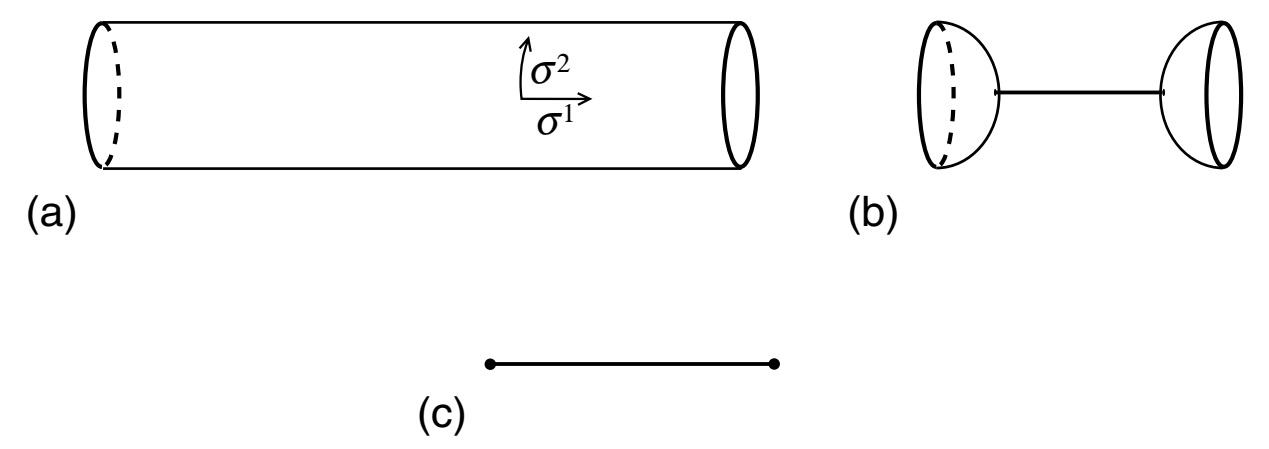
\includegraphics[width=0.8\textwidth,natwidth=951.75,natheight=314.3]{Fig7.1.jpg}\\
		\caption{Fig. 7.1. (a) Cylinder in the limit of small $t$. (b) The amplitude separated into disk tadpole amplitudes and a closed string propagator. (c) Analogous field theory graph. The heavy circles represent the tadpoles.}\label{Fig7.1}
	\end{center}
\end{figure}

它看起来像闭弦从真空中出现,传播了一段距离,又消失在真空中. 为了使其更显然,使用模变换 (7.2.44)
\begin{equation}
	\eta(i t)=t^{-1 / 2} \eta(i / t)
\end{equation}
并将变量改成$s=\pi / t$, 结果是
\begin{equation}
	Z_{C_{2}}=i \frac{V_{26} n^{2}}{2 \pi\left(8 \pi^{2} \alpha^{\prime}\right)^{13}} \int_{0}^{\infty} d s \eta(i s / \pi)^{-24}
\end{equation}
用$1 / t$ 重新标度度规,使得圆柱有闭弦周长 $2 \pi$, 圆柱长度是 $s $. 展开
\begin{equation}
	\begin{aligned}
		\eta(i s / \pi)^{-24} &=\exp (2 s) \prod_{n=1}^{\infty}[1-\exp (-2 n s)]^{-24} \\
		&=\exp (2 s)+24+O(\exp (-2 s))
	\end{aligned}
\end{equation}
这正是用闭弦完备基展开的预期渐近形式. 换句话说,如果我们认为 $\sigma^{2}$ 是世界面时间, $\sigma^{1}$是世界面距离,图(\ref{Fig7.1}a)是一个非常短的开弦圈. 如果我们交换二者的角色,它是一个非常长的闭弦世界线,开端和末端都在边界圆上. 在Euclidean路径积分中,两种描述均可使用,并且在模空间的不同极限下,二者都很有用.\\
真空振幅的领头阶贡献来自闭弦快子. 这是无趣的,它可以通过解析延拓定义
\begin{equation}
	\int_{0}^{\infty} d s \exp (\beta s) \equiv-\frac{1}{\beta}
\end{equation}
第二项来自无质量闭弦态,即使有了延拓也给出形如 $1 / 0$ 的发散. 为了看到这一发散的起源,像图(\ref{Fig7.1}b)那样将过程解离. 正如我们在6.6节看到的,这是在圆盘上有一闭弦顶点算符的非零振幅. 蝌蚪图对应于闭弦消失或出现在真空中. 在动量空间中,无质量传播子正比于 $1 / k^{2} $ . 这里,动量守恒要求从真空中出现的闭弦动量为零,所以传播子发散.\\
在量子场论也有相同类型发散. 考察无质量标量场 $\phi$ 且在Lagrangian中有 $\phi$ 的线性项. 那么就会有只与一个传播子相连的顶点,并且图(\ref{Fig7.1}c)存在. 这一发散是由于中间传播子是
\begin{equation}
	\left.\frac{1}{k^{2}}\right|_{k^{\mu}=0}
\end{equation}
由于传播子极点对应的是传播的时空距离很长,这是长程 (IR) 发散.\\
量子场论中的UV(紫外)发散和IR(红外)发散有着非常不同的起源. UV发散通常标志着理论的失效,在某个短程处需要新物理. IR发散通常意味着我们问出的问题是错误的,或者展开的方式是错误的. 这里也是如此. 在一般微扰论中,我们围绕 $\phi(x)=0$展开或者某个其他场构型展开. 对于作用量
\begin{equation}
	-\frac{1}{g^{2}} \int d^{d} x\left(\frac{1}{2} \partial_{\mu} \phi \partial^{\mu} \phi+g \Lambda \phi\right)
\end{equation}
运动方程
\begin{equation}
	\partial^{2} \phi=g \Lambda
\end{equation}
不允许 $\phi(x)=0$ 作为解. 我们必须围绕 (7.4.8)的一个解展开;而任何解必须是位置相关的. 相应的振幅是没有发散的,即使右边是一微扰 (我们给圆盘引入了合乎的因子 $g$ ), 由于它是奇异微扰,这是正确的. 特别地,正确背景破坏零阶解的某些Poincare对称性.\\
情况在弦论中是相同的. 圆盘蝌蚪图是源
\begin{equation}
	-\Lambda \int d^{26} x(-G)^{1 / 2} e^{-\tilde{\Phi}}
\end{equation}
它是伸缩子和度规的源. 围绕相应场方程的解(不再是常数) 会给出有效的振幅. 细节有一些复杂,将在第9章进一步讨论.\\
附带地,在超弦理论中,如果树图级背景在超对称下不变,那么它通常没有圈修正.\\
极点 (7.4.6) 是我们在树图振幅中遇到了同类发散,对应长时空距离传播的共振. 如果我们在圆柱的每一端加开弦顶点算符,使得它代表开弦一圈振幅,那么从一个边界流向另一个边界的动量 $k^{\mu}$ 一般不为零. 那么大s极限 (7.4.4)会引入因子
\begin{equation}
	\exp \left(-\alpha^{\prime} k^{2} s / 2\right)
\end{equation}
发散变成一个动量极点,它表示开弦散射成闭弦中间态. 因此,正如第3章宣称的,开弦理论必须同时纳入闭弦. 移除UV发散的机制在开弦和闭弦中不同. 在闭弦中是模积分上的有效截断;在开弦,以长时空距离的形式,它重新解释为模空间的危险极限.\\
在 (7.4.1) 中,通过将 $\sigma^{2}$当作时间剪开路径积分,我们将圆柱上的路径积分与开弦频谱关联起来. 它也可通过闭弦获得,这时 $\sigma^{1}$ 是时间. 令 $\sigma^{2}$ 拥有周期$2 \pi$ ,$\sigma^{1}=0, s$处为边界. 闭弦在 $\sigma^{1}=0$ 以某态 $|B\rangle$出现,然后再 $\sigma^{1}=s $又以同样方式消失. 引入测度插入,那么路径积分正比于
\begin{equation}
	\left\langle B\left|c_{0} b_{0} \exp \left[-s\left(L_{0}+\tilde{L}_{0}\right)\right]\right| B\right\rangle
\end{equation}
$\partial_{1} X^{\mu}, c^{1}$和 $b_{12}$在边界上为零决定了态 $|B\rangle$. 以 Hamiltonian形式,它们必须湮灭 $|B\rangle$, 以Laurent系数的形式
\begin{equation}
	\left(\alpha_{n}^{\mu}+\tilde{\alpha}_{-n}^{\mu}\right)|B\rangle=\left(c_{n}+\tilde{c}_{-n}\right)|B\rangle=\left(b_{n}-\tilde{b}_{-n}\right)|B\rangle=0, \quad \text { all } n
\end{equation}
这给出
\begin{equation}
	|B\rangle \propto\left(c_{0}+\tilde{c}_{0}\right) \exp \left[-\sum_{n=1}^{\infty}\left(n^{-1} \alpha_{-n} \cdot \tilde{\alpha}_{-n}+b_{-n} \tilde{c}_{-n}+\tilde{b}_{-n} c_{-n}\right)\right]|0 ; 0\rangle
\end{equation}
将其用于 (7.4.11) 给出 (7.4.3), 还未决定的是 $|B\rangle$ 的归一化. 这个表示在分析 $t \rightarrow 0$的极限以及闭弦极点时候非常有用.\\
通过比较弦论计算与场论计算我们可以决定圆盘蝌蚪 $\Lambda$, 但在下一章,将其作为一个更一般结果的特殊情况进行处理将会更加方便.\\

\centerline{\Large Klein瓶}
来自Klein瓶的真空振幅是
\begin{equation}
	\begin{aligned}
		Z_{K_{2}} &=\int_{0}^{\infty} \frac{d t}{4 t} \operatorname{Tr}_{c}^{\prime}\left\{\Omega \exp \left[-2 \pi t\left(L_{0}+\tilde{L}_{0}\right)\right]\right\} \\
		&=i V_{d} \int_{0}^{\infty} \frac{d t}{4 t}\left(4 \pi^{2} \alpha^{\prime} t\right)^{-d / 2} \sum_{i \in \mathscr{H}_{c}^{\perp}} \Omega_{i} \exp \left[-2 \pi t\left(h_{i}+\tilde{h}_{i}-2\right)\right]
	\end{aligned}
\end{equation}
其中记号来自圆柱(7.4.1). 与定向理论的环面相比,这有一个额外因子 $\frac{1}{2}$ ,它来自投影算符$\frac{1}{2}(1+\Omega) $ . 由于相同原因,在非定向理论中的环面振幅和圆柱振幅均有一个额外因子 $\frac{1}{2}$ . 也可认为这来自额外的规范不变性 $w \rightarrow \bar{w}$. 为了计算26平坦维中的迹,注意$\Omega$ 的的唯一对角元是那些在左移和右移处于相对态,而这些态的贡献是 $\Omega=+1 $ . 这样,迹实际上只取在一边,这与开弦振幅相同,不同的是权重加倍,这是因为左移与右移贡献相同. 结果是
\begin{equation}
	Z_{K_{2}} \rightarrow i V_{26} \int_{0}^{\infty} \frac{d t}{4 t}\left(4 \pi^{2} \alpha^{\prime} t\right)^{-13} \eta(2 i t)^{-24}
\end{equation}
模 $t$ 与圆柱有着相同的取值范围 $0<t<\infty$ ,所以 $t \rightarrow 0$ 发散是相同的. 同样,$1 / 0$极点可以以闭弦极点的形式有一个长程解释. 为了看到这一点,考察区域
\begin{subequations}
\begin{equation}
0 \leq \sigma^{1} \leq 2 \pi, \quad 0 \leq \sigma^{2} \leq 2 \pi t 
\end{equation}
\begin{equation}
0 \leq \sigma^{1} \leq \pi, \quad 0 \leq \sigma^{2} \leq 4 \pi t
\end{equation}		
\end{subequations}
这两个均是基本域,等价关系
\begin{equation}
	w \cong w+2 \pi \cong-\bar{w}+2 \pi i t
\end{equation}
在(7.4.16a)中,左边缘和右边缘周期等价,而上边缘和下边缘在宇称反演后等价,这解释了带有权重$\Omega $的闭弦圈. 对于(7.4.16b), 等价关系 (7.4.17)同时暗示了
\begin{equation}
	w \cong w+4 \pi i t, \quad w+\pi \cong-(\bar{w}+\pi)+2 \pi i t
\end{equation}
由此得出,区域 (7.4.16b)的上边缘和下边缘周期等价. 在左边缘在平移它的一半长度后,通过该边缘的反演与自身等价. 对于右边缘类似:这是十字帽的定义. 因此我们有了图\ref{Fig7.2}a的解释. \\
\begin{figure}
	\begin{center}
		%width=0.8\textwidth,bb=0 0 1256 248
		%1px=0.75pt
		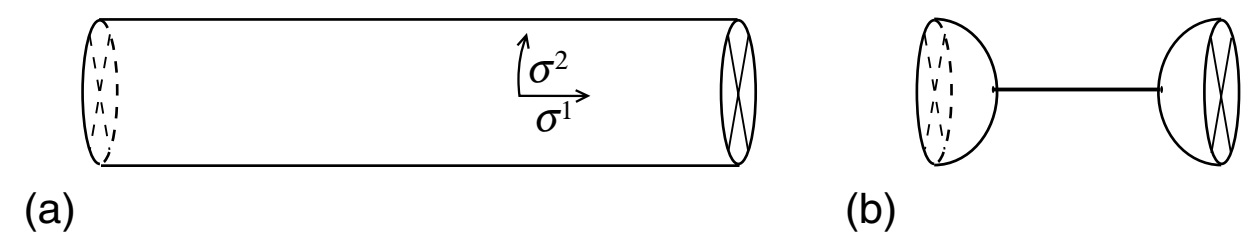
\includegraphics[width=0.8\textwidth,natwidth=879.2,natheight=173.6]{Fig7.2.jpg}\\
		\caption{Fig. 7.2. (a) Klein bottle in the limit of small $t$ as a cylinder capped by crosscaps. (b) The amplitude separated into $R P_{2}$ tadpole amplitudes and a closed string propagator.}\label{Fig7.2}
	\end{center}
\end{figure}

圆柱两端接上十字帽,重新标度$1 / 2 t$, 圆柱底长$2 \pi$,高 $s=\pi / 2 t$. 在模变换后,振幅变成
\begin{equation}
	Z_{K_{2}}=i \frac{2^{26} V_{26}}{4 \pi\left(8 \pi^{2} \alpha^{\prime}\right)^{13}} \int_{0}^{\infty} d s \eta(i s / \pi)^{-24}
\end{equation}

所有关于圆柱的发散的讨论均可用于Klein瓶. 所不同的是蝌蚪图来自于射影平面而非圆盘.\\

\centerline{\Large Möbius带}
对于Möbius带,
\begin{equation}
	Z_{M_{2}}=i V_{d} \int_{0}^{\infty} \frac{d t}{4 t}\left(8 \pi^{2} \alpha^{\prime} t\right)^{-d / 2} \sum_{i \in \mathscr{H}_{0}^{\perp}} \Omega_{i} \exp \left[-2 \pi t\left(h_{i}-1\right)\right]
\end{equation}
它与圆柱上的结果只差 $\Omega$ 以及投影算符的 $\frac{1}{2}$ .在26平坦维中,算符$\Omega$的效应在迹中是:在偶质量能级上有一个额外的$-1$ 再加上对Chan-Paton因子的合理计数. 因此,振子的迹是
\begin{equation}
	\exp (2 \pi t) \prod_{n=1}^{\infty}\left[1-(-1)^{n} \exp (-2 \pi n t)\right]^{-24}=\vartheta_{00}(0,2 i t)^{-12} \eta(2 i t)^{-12}
\end{equation}
对于 $S O(n)$理论, $\frac{1}{2} n(n+1)$ 对称态有$\Omega=+1$,而 $\frac{1}{2} n(n-1)$ 个反对称态有 $\Omega=-1$ ,净贡献为$n$ . 对于$S p(k)$ 理论则相反,给出 $-n$ (在我们的记法中$n=2 k$个 Chan-Paton态). 那么振幅是
\begin{equation}
	Z_{M_{2}}=\pm i n V_{26} \int_{0}^{\infty} \frac{d t}{4 t}\left(8 \pi^{2} \alpha^{\prime} t\right)^{-13} \vartheta_{00}(0,2 i t)^{-12} \eta(2 i t)^{-12}
\end{equation}
通过与Klein瓶相同的构造, Möbius带也可表示为带底的圆柱,这时只有一端是十字帽,如图\ref{Fig7.3}a所示. 

\begin{figure}
	\begin{center}
		%width=0.8\textwidth,bb=0 0 1278 245
		%1px=0.75pt
		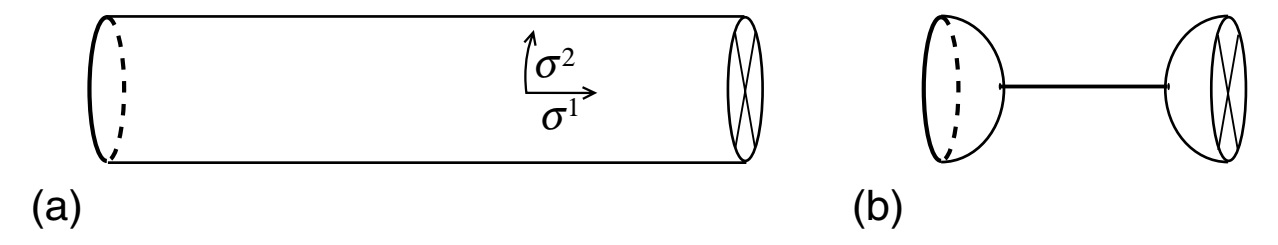
\includegraphics[width=0.8\textwidth,natwidth=894.6,natheight=171.5]{Fig7.3.jpg}\\
		\caption{Fig. 7.3. (a) Möbius in the limit of small $t$ as a cylinder capped by one cross-cap. (b) The amplitude separated into $D_{2}$ and $R P_{2}$ tadpole amplitudes and a closed string propagator.}\label{Fig7.3}
	\end{center}
\end{figure}

圆柱长度现在是$s=\pi / 4 t$. 通过模变换,振幅是
\begin{equation}
Z_{M_{2}}=\pm 2 i n \frac{2^{13} V_{26}}{4 \pi\left(8 \pi^{2} \alpha^{\prime}\right)^{13}} \int_{0}^{\infty} d s \vartheta_{00}(0,2 i s / \pi)^{-12} \eta(2 i s / \pi)^{-12}
\end{equation}
和圆环一样,这也可以写成算符表达式. (7.4.11) 中的一个边界态被替换成了类似的十字帽态 $|C\rangle $ . 这也是 $t \rightarrow 0$ 发散,它对应图\ref{Fig7.3}a的过程,一端来自于圆盘,另一端来自射影平面. 在非定向理论,这三个曲面的发散结合成
\begin{equation}
	i \frac{24 V_{26}}{4 \pi\left(8 \pi^{2} \alpha^{\prime}\right)^{13}}\left(2^{13} \mp n\right)^{2} \int_{0}^{\infty} d s
\end{equation}
即,总的蝌蚪图正比于 $2^{13} \mp n $. 对于规范群 $S O\left(2^{13}\right)=S O(8192)$ 这为零. 来自圆盘的蝌蚪图与来自射影平面的蝌蚪图抵消. 对于玻色弦理论,这或许没什么特殊含义,但在超弦中,对于 $S O(32)$确实有类似的抵消.
% \setcounter{section}{0}%更改chapter的计数器值
% %\numberwithin{equation}{chapter}%公式计数器从属于节计数器
% \numberwithin{equation}{section}%公式计数器从属于节计数器
% \numberwithin{figure}{section}%图计数器从属于节计数器
% \setcounter{chapter}{7}

%\chapter{\texorpdfstring{环面和T对偶}{8 Toroidal compactification and T -duality}}
\chapter{\texorpdfstring{环面和$T$对偶}{环面和T对偶}} \label{cha:8}
弦理论的真实紧致化将是卷II最后几章的主题, 但先来考察一下弦论最简单的紧致化, 一个或多个维度周期等价. 
我们先在场论中考察相同的紧致化, 它们会在规范作用与引力的Kaluza-Klein统一中遇到. 然后我们将其拓展至弦论, 这时产生了几个新的且内禀的弦现象: 
缠绕态, 扩展的规范对称性, $T$对偶以及D膜. 我们还会沿此考察稍微复杂的紧致化, 即轨形(orbifold)与定向形(orientifold).

%\section{\texorpdfstring{场论中的环面紧致化}{8.1 Toroidal compactification in field theory}}
\section{场论中的环面紧致化} \label{sec:8.1}

在广义相对论中, 时空的几何是动力学的. 我们看到的三个空间维是伸展的, 但曾经高度蜷曲. 逻辑上有这样的可能性: 依旧还有保持很小的额外维. 
事实上, 这在1914年就已经提出, 它是一种把电磁场与引力场统一为单个高维场的分量的方法. 考察5维情况, 其中$x^{4}$ 周期等价
\begin{equation}
	x^{4} \cong x^{4}+2 \pi R \:, \label{8.1.1}
\end{equation}
其他$\mu=0,\ldots,3$的$x^{\mu}$ 是不紧致的. 这是环向紧致化, 5维度规分成 $G_{\mu \nu}, G_{\mu 4}$, and $G_{44} $. 从4维观点看, 它们是度规, 矢量以及标量.


我们来细致地考察: 取更普遍的$D=d+1$个时空维的情况, 其中 $x^{d}$ 是周期的. 将度规参数化为
\begin{equation}
	\dif s^{2}=G_{M N}^{D} \dif x^{M} \dif x^{N}=G_{\mu \nu} \dif x^{\mu} \dif x^{\nu}+G_{d d}(\dif x^{d}+A_{\mu} \dif x^{\mu})^{2} \:.
	\label{8.1.2}
\end{equation}
记整个$D$ 维时空的度规为$G_{M N}^{D} $, 注意 $G_{\mu \nu} \neq G_{\mu v}^{D} $; 我们在 $d$ 维作用量中用$G_{\mu \nu} $升降指标. 
现今, 仅允许$G_{\mu \nu}, G_{d d}$及$A_{\mu}$ 依赖于$x^{\mu}$.  \eqref{8.1.2}是在$x^{d}$的平移下不变的最一般形式的度规. 
这一形式依旧允许$d$维再参量化 $x^{\prime \mu}(x^{\nu})$ 以及
\begin{equation}
	x^{\prime d}=x^{d}+\lambda(x^{\mu}) \:. \label{8.1.3}
\end{equation}
在这个再参量化下,
\begin{equation}
	A_{\mu}^{\prime}=A_{\mu}-\partial_{\mu} \lambda \:, \label{8.1.4}
\end{equation}
所以规范变换作为高维坐标群的一部分产生, 这就是 Kaluza-Klein 机制.

为了看到$x^{d}$相关性的效应, 考察$D$维中的无质量标量 $\phi$, 简单起见, 紧致维度中的度规取成 $G_{d d}=1$. 周期维度上的动量是量子化的, $p_{d}=n / R$. 
将 $\phi$对$x^{d}$的依赖展到完备基,
\begin{equation}
	\phi(x^{M})=\sum_{n=-\infty}^{\infty} \phi_{n}(x^{\mu}) \exp (\mi n x^{d} / R) \:. \label{8.1.5}
\end{equation}
$D$维波动方程 $\partial_{M} \partial^{M} \phi=0$ 变成
\begin{equation}
	\partial_{\mu} \partial^{\mu} \phi_{n}(x^{\mu})=\frac{n^{2}}{R^{2}} \phi_{n}(x^{\mu}) \:. \label{8.1.6}
\end{equation}
$D$维场的模 $\phi_{n}$ 因此变成 $d$维场的无限塔. 对于$p_{d} $不为零的场, $d$维质量平方
\begin{equation}
	-p^{\mu} p_{\mu}=\frac{n^{2}}{R^{2}} \label{8.1.7}
\end{equation}
非零. 当能量远小于 $R^{-1}$, 只有 $x^{d}$ 依赖依旧存在, 而物理是$d$ 维的.当能量超过 $R^{-1}$, 我们就看到Kaluza-Klein态塔.

与Kaluza-Klein规范不变性\eqref{8.1.3}相对应的荷是 $p_{d}$ 动量. 在这个简单例子中, 所有携带Kaluza-Klein荷的场都是有质量的. 
更一般地, 若还有高自旋场以及弯曲背景, 那么还有无质量的带荷场.

无质量场的有效作用量总是一个重要课题. 定义 $G_{d d}=\me^{2 \sigma}$,  度规\eqref{8.1.2}的里奇标量是
\begin{equation}
	\bm{R}=\bm{R}_{d}-2 \me^{-\sigma} \nabla^{2} \me^{\sigma}-\frac{1}{4} \me^{2 \sigma} F_{\mu \nu} F^{\mu \nu} \:, \label{8.1.8}
\end{equation}
其中 $\bm{R}$ 是用 $G_{M N}^{D}$ 构造的,  而$\bm{R}_{d}$是用$G_{\mu \nu} $构造的. 引力子-伸缩子作用量\eqref{3.7.20}变成
\begin{align}
	\bm{S}_{1} &= \frac{1}{2 \kappa_{0}^{2}} \int \dif^{D} x \: (-G_{D})^{1/2} \me^{-2 \Phi}(\bm{R}
	 	+4 \nabla_{\mu} \Phi \nabla^{\mu} \Phi) \nonumber \\
		&= \frac{\pi R}{\kappa_{0}^{2}} \int \dif^{d} x\: (-G_{d})^{1/2} \me^{-2 \Phi+\sigma} \nonumber \\
		&\qquad \quad \times\left(\bm{R}_{d}-4 \partial_{\mu} \Phi \partial^{\mu} \sigma+
		4 \partial_{\mu} \Phi \partial^{\mu} \Phi-\frac{1}{4} \me^{2 \sigma} F_{\mu \nu} F^{\mu \nu}\right)\nonumber \\
		&= \frac{\pi R}{\kappa_{0}^{2}} \int  \dif^{d} x \:(-G_{d})^{1 / 2} \me^{-2 \Phi_{d}} \nonumber \\
		&\qquad\quad \times\left(\bm{R}_{d}-\partial_{\mu} \sigma \partial^{\mu} \sigma+4 \partial_{\mu} \Phi_{d} \partial^{\mu} \Phi_{d}-\frac{1}{4} \me^{2 \sigma} F_{\mu \nu} F^{\mu \nu}\right) \:, \label{8.1.9}
\end{align}
这给出了所有无质量场的动能项. 这里 $G_{d}$是 $G_{\mu \nu}$的行列式, $\Phi_{d}=\Phi-\sigma / 2$是有效$d$维伸缩子. 
伸缩子动能项的符号错误是虚假的, 因为引力子与度规迹的混合也必须考虑在内. 实现它的最简单方法是\eqref{3.7.25}中的Weyl变换.

场方程并不决定紧致维数的半径:\footnote{
当然, 只有不变半径
\[
	\rho=R \me^{\sigma}
\]	
区分理不等价的解. 我们可以令$R$等于某个方便的值, 例如$\alpha^{\prime 1/2}$, 但保留它一般会更加方便; 通常设$G_{dd}$为1反而会更加方便. 
类似地, 我们可以通过对$\Phi$的一个偏移而设$\kappa_{0}^{2}$为$\alpha'$的幂级数, 但保留它也没有什么坏处.} 对于$\Phi$ 和 $\sigma $ 的任意值, 平坦度规以及常伸缩子是解. 换句话说, $\Phi$和$\sigma$没有势能, 因而这些场必须是无质量的, 很像戈德斯通玻色子. $\Phi$和$\sigma$ 的不同值标记简并构型(或量子理论的态), 并且若态中的场缓慢变化, 那么它的能量只来自于梯度. 它与戈德斯通现象不同之处在于简并态并没有通过任何对称性彼此相关. 在这个玻色理论中, 简并是偶然的, 并且上一节讨论的一圈能量破坏了这个简并. 在超对称理论中, 存在物理上不等价但简并的真空, 这是相当常见的, 并且在理解动力学时有很大作用. 用来标记不等价真空的场被称为模. 在自然中, 超对称破缺几乎必然地赋予了所有模质量, 否则它们将传递引力量级的无限长程力.

定义$A_{\mu}=R \tilde{A}_{\mu}$, 协变导数为
\begin{equation}
	\partial_{\mu}+\mi p_{d} A_{\mu}=\partial_{\mu}+\mi n \tilde{A}_{\mu} \:, \label{8.1.10}
\end{equation}
这使得电荷是整数.  $d$ 维规范耦合与引力耦合的定义如下. 拉格朗日密度中 $\tilde{F}_{\mu \nu} \tilde{F}^{\mu \nu}$的系数定义成 $-1 / 4 g_{d}^{2}$, 
$\bm{R}_{d}$的系数定义成 $1 / 2 \kappa_{d}^{2}$. 以引力耦合的形式, 规范耦合写成
\begin{equation}
	g_{d}^{2}=\frac{\kappa_{0}^{2} \me^{2 \Phi_{d}}}{\pi R^{3} \me^{2 \sigma}}=\frac{2 \kappa_{d}^{2}}{\rho^{2}} \:. \label{8.1.11}
\end{equation}
$d$ 维与 $D$ 维引力耦合关系是
\begin{equation}
	\frac{1}{\kappa_{d}^{2}}=\frac{2 \pi \rho}{\kappa^{2}} \:, \label{8.1.12}
\end{equation}
$2 \pi \rho$ 是紧致维数的体积.
\begin{tcolorbox}
	\begin{remark}
		\begin{itemize}
			\item $1 / g_{d}^{2}$有定义$A_{\mu}=R \tilde{A}_{\mu}$贡献的因子$R^{2}$, 其它的贡献来自于\eqref{8.1.9}, 再加上 $\rho=R\me^{\sigma}$ 就给出了\eqref{8.1.11}.
			\item 根据\eqref{8.1.9}和定义, $1 / 2 \kappa_{d}^{2}=\frac{\pi R \me^{-2 \Phi_d}}{\kappa_{0}^{2}}$. 而$D$维引力耦合是$\frac{1}{2 \kappa^{2}}=\frac{\me^{-2 \Phi}}{2 \kappa_{0}^{2}}$, 由此给出\eqref{8.1.12}
		\end{itemize}
	\end{remark}
\end{tcolorbox}

% \fbox{\noindent\centering\parbox{0.9\textwidth}{Note:
% 		$$1 / g_{\alpha}^{2}=R^{2} e^{2 \sigma} \cdot \frac{\pi R}{k_{0}^{2}} e^{-2 {\Phi}_{d}},\quad 1 / 2 k_{d}^{2}=\frac{\pi R e^{-2 \Phi_d}}{k_{0}^{2}},\quad \rho=R e^\sigma$$}}\\


% \fbox{\noindent\centering\parbox{0.9\textwid$th}{Note:
% 		$\frac{1}{2 k^{2}}=\frac{e^{-2 \Phi}}{2 k_{0}^{2}}=\frac{e^{-2 \Phi}}{2} \frac{1}{2 k_{d}^{2} \pi R e^{-2{\Phi} _d}}=\frac{e^{-\sigma}}{4 k_{d}^{2} \pi R}=\frac{1}{2 k_{d}^{2} 2 \pi \rho}$$}}\\

通过推广Kaluza-Klein机制, 反对称张量也可以给出规范对称性. 将 $B_{M N}$ 分成 $B_{\mu \nu}$和$A_{\mu}^{\prime}=B_{d \mu}$, 
\eqref{3.7.7}中的规范参量 $\zeta_{M}$ 分成 $d$维反对称张量变换 $\zeta_{\mu}$和普通的规范不变量 $\zeta_{d}$. 
规范场是 $B_{d \mu}$, 场强是 $H_{d \mu \nu}$. 反对称张量作用量变成
\begin{align}
	\bm{S}_{2} &=-\frac{1}{24 \kappa_{0}^{2}} \int \dif^{D} x \:(-G_{D})^{1 / 2} \me^{-2 \Phi} H_{M N L} H^{M N L} \nonumber \\
	&=-\frac{\pi R}{12 \kappa_{0}^{2}} \int \dif^{d} x \: (-G_{d})^{1/2} \me^{-2 \Phi_{d}}
	\Bigl(\tilde{H}_{\mu \nu \lambda} \tilde{H}^{\mu \nu \lambda}+3 \me^{-2 \sigma} H_{d \mu \nu} H_{d}^{\mu \nu}\Bigr) \:. \label{8.1.13}
\end{align}
我们定义了
\begin{equation}
	\tilde{H}_{\mu \nu \lambda}=(\partial_{\mu} B_{\nu \lambda}-A_{\mu} H_{d \nu \lambda})+\text{循环置换} \:. \label{8.1.14}
\end{equation}
正比于矢势的项来源于逆度规 $G^{M N} $. 它被称为 Chern-Simons 项, 这代表一个规范势与任意多个场强相耦合. 
在超对称理论中经常会出现这样的项, 并与有趣的物理现象相联系. 注意 $\tilde{H}_{\mu \nu \lambda}$ 是规范不变的, 
这是因为$A_{\mu}$的变分\eqref{8.1.4}被如下变分抵消: 
\begin{equation}
	B_{\nu \lambda}^{\prime}=B_{\nu \lambda}-\lambda H_{d \nu \lambda} \:. \label{8.1.15}
\end{equation}

不存在 $B_{M N}$与其他场的最小耦合, 所以不像Kaluza-Klein情况. 在反对称张量规范对称性下没有场带荷; 在弦论中这是不同的.
\begin{tcolorbox}
	\begin{remark}
		逆度规是
		\[
		g^{MN}=\begin{bmatrix}
			g^{\mu \nu} & -A^{\mu} \\
            -A^{\nu} & g_{\mu \nu} A^{\mu} A^{\nu}+\me^{-2 \sigma}
		\end{bmatrix}	 \:.
		\]
		% \eqref{8.1.13}来自于
		% \begin{align*}
		% 		G^{M W} G^{L K} G^{S R} H_{M L S} H_{N K R}&=3 G^{d d} H_{d \mu \nu} H_{d \mu \nu} \\
		% 		&=3 \me^{-2 \sigma} H_{d \mu \nu} H_{d}^{\mu \nu}+3 g_{\mu \nu} A_{\mu } H_{d\mu \nu}+A_{\nu} H_{d}^{\mu \nu}
		% \end{align*}
	\end{remark}
\end{tcolorbox}


\section{共形场论中的环面紧致化} \label{sec:8.2}%{8.2 Toroidal compactification in CFT}

现在我们来考察单个周期标量场的共形场论,
\begin{equation}
	X \cong X+2 \pi R \:. \label{8.2.1}
\end{equation}
为了保持方程的整洁, 我们扔掉$X^{d}$的上标, 并令 $G_{d d}=1$. 世界面作用量与非紧致理论相同, 均为 $\int \dif^{2} z \,\partial X \bar{\partial} X / 2 \pi \alpha^{\prime}$, 所以运动方程, 算符乘积以及能动张量均保持不变. 周期性有两个效应. 其一, 弦态在等价关系\eqref{8.2.1}下必须是单值的. 
即, 平移弦的算符$\exp(2\pi\mi p)$绕紧致维数一圈必须使该态不变, 所以质心动量量子化
\begin{equation}
	k=\frac{n}{R}, \quad n \in \mathds{Z} \:. \label{8.2.2}
\end{equation}
这与场论相同.


\begin{figure}[h]
	\begin{center}
		%width=0.8\textwidth,bb=0 0 1052 545
		%1px=0.75pt
		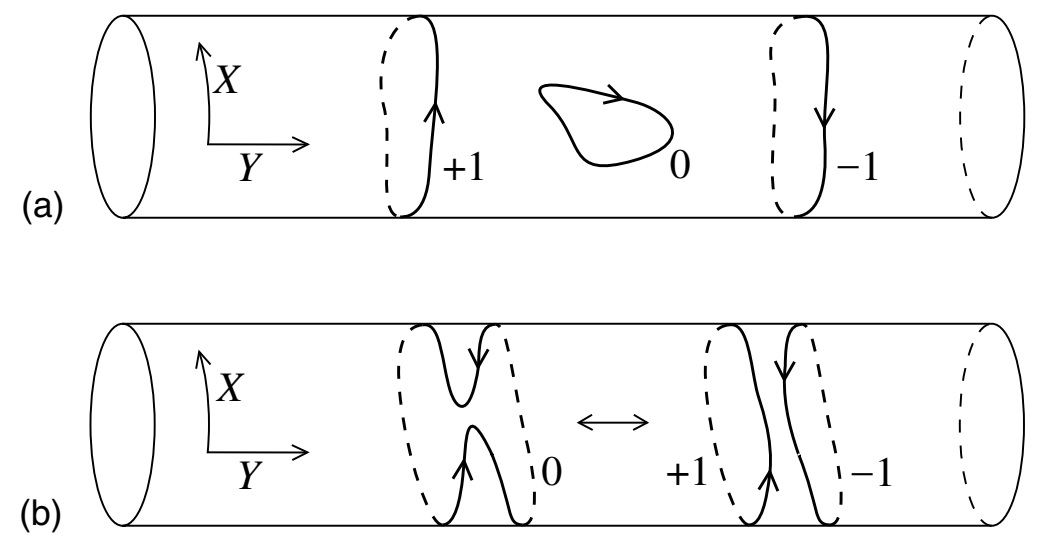
\includegraphics[width=0.8\textwidth,natwidth=789,natheight=408.75]{Fig8.1.jpg}\\
		\caption{(a) 缠绕数为$w=+1,0,-1$的定向闭弦. (b) $w=0$的弦跃迁至 $w=+1$ 和 $w=-1$ 的弦.}\label{Fig8.1}
	\end{center}
\end{figure}


其二为弦论特有. 闭弦现在必须缠绕紧致维,
\begin{equation}
	X(\sigma+2 \pi)=X(\sigma)+2 \pi R w, \quad w \in \mathds{Z} \:. \label{8.2.3}
\end{equation}
整数 $w$ 是缠绕数. 缠绕数为 $+1, 0 ,-1$的态如图\ref{Fig8.1}(a)所示.
从世界面场论的观点来看, 缠绕数非零的弦是拓扑孤子, 即场构型拓扑非平庸的态. 相容的弦理论必须纳入缠绕数态: 通过分裂-合并过程, 
$w=0$ 的弦可以变成 $w=+1$, $w=-1$ 的弦, 如图\ref{Fig8.1}(b)所示. 很容易看到这个例子中缠绕数总是守恒的. 

为了确定闭弦 CFT 的态, 考察洛朗展开
\begin{equation}
	\partial X(z)=-\mi\left(\frac{\alpha^{\prime}}{2}\right)^{1 / 2} \sum_{m=-\infty}^{\infty} \frac{\alpha_{m}}{z^{m+1}}\:, \qquad 
	\bar{\partial} X(\bar{z})=-\mi\left(\frac{\alpha^{\prime}}{2}\right)^{1 / 2} \sum_{m=-\infty}^{\infty} \frac{\tilde{\alpha}_{m}}{\bar{z}^{m+1}} \:. \label{8.2.4}
\end{equation}
缠绕一周后, $X$的改变为
\begin{equation}
	2 \pi R w=\oint(\dif z\: \partial X + \dif \bar{z}\: \bar{\partial} X)= 2 \pi(\alpha^{\prime}/2)^{1/2}(\alpha_{0}-\tilde{\alpha}_{0}) \:. \label{8.2.5}
\end{equation}
总的诺特动量是
\begin{equation}
	p=\frac{1}{2 \pi \alpha^{\prime}} \oint(\dif z\: \partial X- \dif \bar{z}\: \bar{\partial} X)
	=(2 \alpha^{\prime})^{-1 / 2}(\alpha_{0}+\tilde{\alpha}_{0}) \:. \label{8.2.6}
\end{equation}
对于非紧致维度, 这像往常一样给出 $\alpha_{0}=\tilde{\alpha}_{0}=p(\alpha^{\prime} / 2)^{1 / 2}$, 但对于周期维度则有
\begin{subequations} \label{8.2.7}
\begin{align}
p_{L} \equiv\left(2 / \alpha^{\prime}\right)^{1 / 2} \alpha_{0}=\frac{n}{R}+\frac{w R}{\alpha^{\prime}} \:, \label{8.2.7a} \\
p_{R} \equiv\left(2 / \alpha^{\prime}\right)^{1 / 2} \tilde{\alpha}_{0}=\frac{n}{R}-\frac{w R}{\alpha^{\prime}} \:. \label{8.2.7b}
\end{align}		
\end{subequations}
Virasoro生成元是
\begin{subequations} \label{8.2.8}
\begin{align}
L_{0}&=\frac{\alpha^{\prime} p_{L}^{2}}{4}+\sum_{n=1}^{\infty} \alpha_{-n} \alpha_{n} \:, \label{8.2.8a} \\
\tilde{L}_{0}&=\frac{\alpha^{\prime} p_{R}^{2}}{4}+\sum_{n=1}^{\infty} \tilde{\alpha}_{-n} \tilde{\alpha}_{n} \:. \label{8.2.8b}
\end{align}		 				
\end{subequations}


\subsection*{配分函数}
 $X$ 的配分函数
	\begin{align}
		&(q \bar{q})^{-1 / 24} \operatorname{Tr}\Bigl(q^{L_{0}} \bar{q}^{\tilde{L}_{0}}\Bigr) \nonumber \\
		&\quad =|\eta(\tau)|^{-2} \sum_{n, w=-\infty}^{\infty} q^{\alpha^{\prime} p_{L}^{2} / 4} \bar{q}^{\alpha^{\prime} p_{R}^{2} / 4} \nonumber \\
		&\quad =|\eta(\tau)|^{-2} \sum_{n, w=-\infty}^{\infty} \exp \left[-\pi \tau_{2}\left(\frac{\alpha^{\prime} n^{2}}{R^{2}}+\frac{w^{2} R^{2}}{\alpha^{\prime}}\right)+2 \pi \mi \tau_{1} n w\right] \:. \label{8.2.9}
	\end{align}
振子与非紧致情况相同, 而动量积分被换成了对$n$ 和 $w$的求和. 模不变性不显然, 但利用Poisson重求和公式,
\begin{equation}
	\sum_{n=-\infty}^{\infty} \exp (-\pi a n^{2}+2 \pi \mi b n)=a^{-1 / 2} 
	\sum_{m=-\infty}^{\infty} \exp \biggl[-\frac{\pi(m-b)^{2}}{a}\biggr] \:. \label{8.2.10}
\end{equation}
配分函数变成
\begin{equation}
	2 \pi R Z_{X}(\tau) \sum_{m, w=-\infty}^{\infty} \exp \biggl(-\frac{\pi R^{2}|m-w \tau|^{2}}{\alpha^{\prime} \tau_{2}}\biggr) \:. \label{8.2.11}
\end{equation}
% \fbox{\noindent\centering\parbox{0.9\textwidth}{Note:
% $$
% \begin{aligned}
% &\sum_{n=-\infty}^{+\infty} \exp \left[-\pi \tau_{2} \frac{\alpha^{\prime} n^{2}}{R^{2}}+2 \pi i \tau_{1} n w-\pi \tau_{2}  \frac{w^{2} R^{2}}{\alpha^{\prime}}\right] \\
% &=\frac{R}{\left(\alpha^{\prime} \tau_{2}\right)^{1 / 2}} \sum_{m=-\infty}^{+\infty} \exp \left[-\frac{\pi R^{2}}{\alpha^{\prime} \tau_{2}}\left(\left(m-w \tau_{1}\right)^{2}+w^{2} \tau_{2}^{2}\right)\right]
% \end{aligned}
% $$
% $$
% Z_{x}(\tau)=\frac{|\eta(\tau)|^{-2}}{\left(4 \pi^{2} \alpha^{\prime} \tau_{2}\right)^{1 / 2}}
% $$}}\\
$Z_{X}(\tau)$是非紧致理论中的模不变表达式\eqref{7.2.9}, 这个和在 $\tau \rightarrow \tau+1$下显然是不变的. 而当$\tau \rightarrow-1 / \tau$ 时, 它在$m\to-w$和$w\to m$下不变.

\begin{tcolorbox}
	\begin{remark}
		在$\tau \to -1/\tau$下, 
		\[
			\frac{|m-w \tau|^{2}}{\tau_{2}} \rightarrow \frac{| m+w / \tau|^{2}}{\tau_{2} /|\tau|^{2}}=\frac{|m \tau+w|^{2}}{\tau_{2}}	
		\]
	\end{remark}
\end{tcolorbox}


\eqref{8.2.11} 有一个简单的路径积分解释. 在周期时空中对所有亏格为1的世界面求和, 世界面上每个不平庸的闭曲线会缠绕紧致方向
\begin{subequations} \label{8.2.12}
\begin{align}
X(\sigma^{1}+2 \pi, \sigma^{2}) &= X(\sigma^{1}, \sigma^{2})+2 \pi w R \:, \label{8.2.12a} \\
X(\sigma^{1}+2 \pi \tau_{1}, \sigma^{2}+2 \pi \tau_{2}) &= X(\sigma^{1}, \sigma^{2})+2 \pi m R \:. \label{8.2.12b} 
\end{align}
\end{subequations}
即, 路径积分分裂成由$w$ 和 $m $标记的拓扑不等价截面. 通过将$X$写成满足周期性的经典解                                                                                                              
\begin{equation}
	X_{\mathrm{cl}}=\sigma^{1} w R+\sigma^{2}(m-w \tau_{1}) R / \tau_{2} \:, \label{8.2.13}
\end{equation}
加上满足周期性边界条件的量子部分. 这个高斯型路径积分可以积掉. 对量子部分的路径积分与非紧致情况相同, 而经典部分作为\eqref{8.2.11}中的指数出现. 
模变换在周期性上的效应就简化为交换求和变量 $m$ 和 $w$.

\subsection*{顶点算符}
为了构造 $\alpha_{0} \neq \tilde{\alpha}_{0}$的缠绕态, 我们需要独立的变量 $x_{L}$和 $x_{R}$, 满足
\begin{equation}
	[x_{L}, p_{L}]=[x_{R}, p_{R}]=\mi \:. \label{8.2.14}
\end{equation}
场 $X$ 分裂成称全纯部分和反全纯部分
\begin{equation}
	X(z, \bar{z})=X_{L}(z)+X_{R}(\bar{z}) \:, \label{8.2.15}
\end{equation}
其中
\begin{subequations} \label{8.2.16}
\begin{align}
X_{L}(z) &= x_{L}- \mi \frac{\alpha^{\prime}}{2} p_{L} \ln z+\mi\left(\frac{\alpha^{\prime}}{2}\right)^{1 / 2} 
			\sum_{\substack{m=-\infty  \\  m \neq 0}}^{\infty} \frac{\alpha_{m}}{m z^{m}} \:, \label{8.2.16a} \\
X_{R}(\bar{z})&= x_{R}-\mi \frac{\alpha^{\prime}}{2} p_{R} \ln \bar{z}+\mi\left(\frac{\alpha^{\prime}}{2}\right)^{1 / 2} 
\sum_{\substack{m=-\infty  \\  m \neq 0}}^{\infty} \frac{\tilde{\alpha}_{m}}{m \bar{z}^{m}} \:. \label{8.2.16b}
\end{align}
\end{subequations}
如果我们限制在 $k_{L}=k_{R}$的态上且只用 $X_{L}(z)+X_{R}(\bar{z})$构建的算符, 这就退化至非紧致维度的CFT.

我们现在讨论OPE与顶点算符. 很容易猜出顶点算符的形式, 既然通常的$XX$算符乘积 $-(\alpha^{\prime} / 2) \ln (z_{12} \bar{z}_{12})$可以拆成全纯函数和反全纯函数, 因此
\begin{subequations} \label{8.2.17}
\begin{align}
X_{L}(z_{1}) X_{L}(z_{2}) &\sim-\frac{\alpha^{\prime}}{2} \ln z_{12}, \quad 
X_{R}(\bar{z}_{1}) X_{R}(\bar{z}_{2}) \sim-\frac{\alpha^{\prime}}{2} \ln \bar{z}_{12}  \:,  \label{8.2.17a} \\
X_{L}(z_{1}) X_{R}(\bar{z}_{2}) &\sim 0 \:. \label{8.2.17b}
\end{align}		
\end{subequations}
对应于态 $|0 ; k_{L}, k_{R}\rangle$的算符是
\begin{equation}
	\mathscr{V}_{k_{L} k_{R}}(z, \bar{z}) = : \mathrel{e^{\mi k_{L} X_{L}(z)+ \mi k_{R} X_{R}(\bar{z})}}: \label{8.2.18}
\end{equation}
OPE为
\begin{equation}
	\mathscr{V}_{k_{L} k_{R}}(z_{1}, \bar{z}_{1}) \mathscr{V}_{k_{L}^{\prime} k_{R}^{\prime}}(z_{2}, \bar{z}_{2}) \sim 
	z_{12}^{\alpha^{\prime} k_{L} k_{L}^{\prime} / 2} \bar{z}_{12}^{\alpha^{\prime} k_{R} k_{R}^{\prime} / 2} 
	\mathscr{V}_{(k+k^{\prime})_{L}(k+k^{\prime})_{R}}(z_{2}, \bar{z}_{2}) \:. \label{8.2.19}
\end{equation}
我们会在各种表达式中遇到支点、割线, 这不奇怪, 因为场$X$不再是单值的. 然而重要的是, 整个顶点算符的OPE必须是单值的: 当 $z_{1}$ 环绕 $z_{2}$一周, 净相位为1.
\begin{equation}
	\exp [\pi \mi \alpha^{\prime}(k_{L} k_{L}^{\prime}-k_{R} k_{R}^{\prime})]
	=\exp [2 \pi \mi(n w^{\prime}+w n^{\prime})]=1 \:. \label{8.2.20}
\end{equation}
为了使弦振幅合理定义, 这正是所必须的.

% \fbox{\noindent\centering\parbox{0.9\textwidth}{Note:
% 		$$
% 		k_{L} \cdot k_{L}^{\prime}=\left(\frac{n}{R}+\frac{w R}{\alpha^{\prime}}\right)\left(\frac{n^{\prime}}{R}+\frac{w^{\prime} R}{\alpha^{\prime}}\right)=\frac{n n^{\prime}}{R^{2}}+\frac{w^{\prime} n}{\alpha^{\prime}}+\frac{n w^{\prime} }{\alpha^{\prime}}+\frac{w w^{\prime} R^2}{(\alpha^\prime)^2}
% 		$$
% 	$$
% 	k_{R} \cdot k_{R}^{\prime}=\left(\frac{n}{R}-\frac{w R}{\alpha^{\prime}}\right)\left(\frac{n^{\prime}}{R}-\frac{w^{\prime} R}{\alpha^{\prime}}\right)=\frac{n n^{\prime}}{R^{2}}-\frac{w^{\prime} n}{\alpha^{\prime}}-\frac{n w^{\prime} }{\alpha^{\prime}}+\frac{w w^{\prime} R^2}{(\alpha^\prime)^2}
% 	$$
% $$
% \alpha^{\prime}\left(k_{L} \cdot k_{L}^{\prime}-k_{R} k_{R}^{\prime}\right)=2 w^{\prime} n+2 n w^{\prime}
% $$}}\\


\subsection*{一个技巧}

前面的讨论显然是正确的, 但我们对于对数中支点、割线位置的处理太过随便. 如果我们交换$z_{1}$ 和 $z_{2}$, 以及动量 $k$ 和 $k^{\prime} $, 
OPE\eqref{8.2.19}就会出现问题. 左边是对称的, 但右边会差 $\exp[\pi \mi(n w^{\prime}+w n^{\prime})]$. 因此, 
如果 $n w^{\prime}+w n^{\prime}$为奇, 会差一个负号. 我们也可以以如下方式看到这个问题. 从模展开可导出等时 $(|z_{1}|=|z_{2}|)$ 对易子
\begin{equation}
	[X_{L}(z_{1}), X_{L}(z_{2})]=\frac{\pi \mi \alpha^{\prime}}{2} \operatorname{sign}(\sigma_{1}^{1}-\sigma_{2}^{1}) \:. \label{8.2.21}
\end{equation}
那么CBH公式告诉我们, 如果我们通过产生-湮灭次序定义算符, 那么$n w^{\prime}+w n^{\prime}$ 为奇时, 算符 $\mathscr{V}_{k_{L} k_{R}}$ 与 $\mathscr{V}_{k_{k}^{\prime} k_{R}^{\prime}}$反对易; 不可见的支点、割线\eqref{8.2.20}会变成两个可视的. 顶点算符正确的振子表达式是(相位中有任意性) 
\begin{equation}
	\mathscr{V}_{k_{L} k_{R}}(z, \bar{z})=\exp [\pi \mi(k_{L}-k_{R})(p_{L}+p_{R}) \alpha^{\prime} / 4] 
	\mathrel{\typecolon \me^{\mi k_{L} X_{L}(z)+\mi k_{R} X_{R}(\bar{z})} \typecolon} \:, \label{8.2.22}
\end{equation}
其中像往常一样,  $p_L,p_R$ 是算符, $k$ 是数 (给定顶点算符携带的动量). 
当 $\mathscr{V}_{k_{L} k_{R}}$和 $\mathscr{V}_{k_{L}^{\prime} k_{R}^{\prime}}$彼此对易时, 额外的因子称为闭上链(cocycles), 这给出额外相位
\begin{align}
	\exp \Bigl\{\pi \mi\Bigl[(k_{L}-k_{R})(k_{L}^{\prime}+k_{R}^{\prime})-(k_{L}^{\prime}-k_{R}^{\prime})(k_{L}+k_{R})\Bigr] 
	\alpha^{\prime} / 4\Bigr\}\quad &  \nonumber \\
	=\exp [\pi \mi(n w^{\prime}-w n^{\prime})] &\:, \label{8.2.23}
\end{align}
这移除了支点、割线. 对于大多数情况, 可以忽视这一复杂性, 并用上一段那个更简单的表达式进行处理; 闭上链只影响特定振幅的相对符号.

一般的 $X^{\mu}$ 路径积分 \eqref{6.2.18} 以一种显然的方式因式分解成全纯和反全纯的, 这使得我们可以做替换
\begin{equation}
	\prod_{i<j}^{n}|z_{i j}|^{\alpha^{\prime} k_{i} k_{j}} \to \prod_{i<j}^{n} z_{i j}^{\alpha^{\prime} k_{L i} k_{L j} / 2} 
	\bar{z}_{i j}^{\alpha^{\prime} k_{R i} k_{R j} / 2} \:, \label{8.2.24}
\end{equation}
也可将来自 $x_{0}$的非紧致积分的 $2 \pi \delta(\sum k)$ 换成
\begin{equation}
	2 \pi R \delta_{\Sigma_{i} n_{i}, 0} \delta_{\Sigma_{i} w_{i}, 0} \:. \label{8.2.25}
\end{equation}
精确表达式 \eqref{8.2.22} 会给出一些额外的符号.

\subsection*{DDF算符}

我们已经看到指数算符可以分成全纯和反全纯部分, 这有很多应用, 我们现在用它来讨论第4章末尾的DDF算符.

我们将用光锥坐标 $X^{\pm}=2^{-1 / 2}(X^{0} \pm X^{1})$处理, 它的全纯部分有 OPE(扔掉下标 $L$)
\begin{equation}
	X^{+}(z) X^{-}(0) \sim \frac{\alpha^{\prime}}{2} \ln z, \qquad X^{+}(z) X^{+}(0) \sim X^{-}(z) X^{-}(0) \sim 0 \:. \label{8.2.26}
\end{equation}
\begin{tcolorbox}
	\begin{remark}
		\begin{align*}
X^{+}(z) X^{-}(0) &=2^{-1}\left(X^{0}(z)+X^{\prime}(z)\right)\left(X^{0}(0)-X^{\prime}(0)\right) \\
&=2^{-1}\left(\frac{\alpha^{\prime}}{2} \ln z_{12}+\frac{\alpha^{\prime}}{2}\ln z_{12}\right)=\frac{\alpha^{\prime}}{2} \ln z_{12} \:.
		\end{align*}
	\end{remark}
\end{tcolorbox}
\noindent 由此得出算符
\begin{equation}
	V^{i}(n k_{0}, z)=\partial X^{i}(z) \me^{\mi n k_{0} X^{+}(z)}(2 / \alpha^{\prime})^{1 / 2} \label{8.2.27}
\end{equation}
是$(1,0)$本原场, 其中$i$是横向指标. OPE 为
\begin{align}
	V^{i}(n k_{0}, z) V^{j}(m k_{0}, 0) &\sim-\frac{\delta^{i j}}{z^{2}} \me^{\mi(n+m) k_{0} X^{+}(0)}  \nonumber \\
	&\quad -\frac{\mi n k_{0} \delta^{i j}}{z} \partial X^{+}(0) \me^{\mi(n+m) k_{0} X^{+}(0)} \:. \label{8.2.28}
\end{align}
定义DDF算符为
\begin{equation}
	A_{n}^{i}=\oint \frac{\dif z}{2 \pi} \, V^{i}(n k_{0}, z) \:. \label{8.2.29}
\end{equation}
除非$n+m=0$, 否则OPE\eqref{8.2.28}中的 $z^{-1}$ 项就是全导数, 因而 DDF 算符满足振子代数
\begin{equation}
	[A_{m}^{i}, A_{n}^{j}]=m \delta^{i j} \delta_{m,-n} \frac{\alpha^{\prime} k_{0} p^{+}}{2} \:. \label{8.2.30}
\end{equation}

考察这个算符在动量给定为 $q$的态上的作用.  $V^{i}(n k_{0}, z)$ 与这个态的顶点算符将会包含 $z^{-\alpha^{\prime} n k_{0} q^{-} / 2}$. 
因而如果我们固定$k_{0}=2 / \alpha^{\prime} q^{-}$, 它将是单值的. 那么围道积分\eqref{8.2.29}就在这个截面上定义了合理的算符. 
DDF 算符是 $(1,0)$张量的积分, 因而与Virasoro生成元对易, 它将物理态变到物理态. 由此, 我们可以通过用 DDF 算符作用振子基态建立物理态. 
以这种方法得到的态与光锥态一一对应. DDF算符不包含$X^{-}$, 因而这些态没有 $\alpha_{-m}^{-}$激发. 
因此, 与更加一般但不太显然的构造\eqref{4.4.19}相比, 它们实际上给出相同的态.


\section{闭弦和T对偶} \label{sec:8.3}%{8.3 Closed strings and T -duality}

既然我们在研究弦理论, 我们取 $D=26$, 并且只取 $X^{25}$ 是周期的. 质壳 ($L_{0}$与$\tilde{L}_{0}$) 是
	\begin{align}
		m^{2}=-k^{\mu} k_{\mu} &= (k_{L}^{25})^{2}+\frac{4}{\alpha^{\prime}}(N-1) \nonumber \\
		&=(k_{R}^{25})^{2}+\frac{4}{\alpha^{\prime}}(\tilde{N}-1) \:, \label{8.3.1}
	\end{align}
或
\begin{subequations} \label{8.3.2}
\begin{align}
m^{2} &= \frac{n^{2}}{R^{2}}+\frac{w^{2} R^{2}}{\alpha^{\prime 2}}+\frac{2}{\alpha^{\prime}}(N+\tilde{N}-2) \:, \label{8.3.2a} \\
0 &= n w+N-\tilde{N} \:. \label{8.3.2b} 
\end{align}
\end{subequations}
对质量平方有四个贡献: 紧致动量, 缠绕弦的势能, 振子以及零点能. 第\ref{cha:4}章对物理频谱的讨论适用于任何紧致化, 
所以我们仅通过考察横向振子 $M=2, \ldots, 25$, 就得到了态的正确计数.

首先, 我们复现出无质量频谱的场论结果. 在$R$的一般值处, 仅当$n=w=0$, $N=\tilde{N}=1$时, 态才可能是无质量的. 这里有 $24^{2}$个相同的态, 但是根据振子是处在时空方向 $\mu$还是内部方向25, 对其分类将是有用的:
\begin{align}
	&\alpha_{-1}^{\mu} \tilde{\alpha}_{-1}^{\nu}|0 ; k\rangle\:, \qquad 
	(\alpha_{-1}^{\mu} \tilde{\alpha}_{-1}^{25}+\alpha_{-1}^{25} \tilde{\alpha}_{-1}^{\mu})|0 ; k\rangle \:, \nonumber \\
	&(\alpha_{-1}^{\mu} \tilde{\alpha}_{-1}^{25}-\alpha_{-1}^{25} \tilde{\alpha}_{-1}^{\mu})|0 ; k\rangle\:, \qquad 
	\alpha_{-1}^{25} \tilde{\alpha}_{-1}^{25}|0 ; k\rangle \:. \label{8.3.3}
\end{align}
其中第一个进一步分裂成25维引力子加伸缩子加反对称张量. 第二个, 时空维度与内部指标上的引力子, 它是Kaluza-Klein矢量. 第三个是来自反对称张量的矢量. 
最后一个态是标量, 它是紧致方向上半径的模, 它的顶点算符 $:\mathrel{\partial X^{25} \bar{\partial} X^{25} \me^{\mi k \cdot X}}:$ 是度规 $G_{25,25}$的微扰. 这与考察低能场论时发现的频谱相同.

考察有质量的态在 $U(1) \times U(1)$ 对称性下的变换是十分有益的. 再一次, Kaluza-Klein 规范对称性来自 $X^{25}$ 方向上的平移, 
所以相应的荷是紧致动量 $p_{25} $. 对于反对称张量规范对称性, 考察零动量顶点算符, 它测出了任何与其耦合的态的变换. 它正比于
\begin{equation}
	\partial X^{\mu} \bar{\partial} X^{25}-\partial X^{25} \bar{\partial} X^{\mu}= 
	\bar{\partial}(X^{25} \partial X^{\mu})-\partial(X^{25} \bar{\partial} X^{\mu}) \:. \label{8.3.4}
\end{equation}
这是全导数, 但是在缠绕态上, 由于$X^{25}$不是单值的, 所以它的积分不为零. 所以 $B_{\mu, 25}$荷是缠绕数. 
这是这一紧致化中我们首个遇到的``弦''物理: 在场论中没有携带这一荷的态.

我们从弦三点耦合来验证规范耦合. 规范玻色子顶点算符是
\begin{equation}
	\frac{2^{1 / 2} g_{\mathrm{c}, 25}}{\alpha^{\prime}}:\mathrel{(\partial X^{\mu} \bar{\partial} X^{25} \pm 
	\partial X^{25} \bar{\partial} X^{\mu}) \me^{\mi k \cdot X}}: \:. \label{8.3.5}
\end{equation}
我们将25维弦耦合 $g_{\mathrm{c}, 25}=g_{\mathrm{c}}(2 \pi R)^{-1 / 2}$. 因子 $(2 \pi R)^{-1 / 2}$ 来自于零模波函数的归一化, 
对于一般的紧致动量和缠绕数, 快子的顶点算符是
\begin{equation}
	g_{\mathrm{c}, 25}:\mathrel{ \me^{\mi k_{L} \cdot X_{L}(z)+\mi k_{R} \cdot X_{R}(\bar{z})}}: \:.
\end{equation}
一个规范玻色子与两个快子的三点振幅, 若快子的紧致动量以及缠绕数不为零, 那么类似于\eqref{6.6.14},
\begin{align}
	& {-}2^{-1 / 2} \pi \mi g_{\mathrm{c}, 25}(2 \pi)^{25} \delta^{25}({\textstyle\sum_{i} k_{i}}) k_{23}^{\mu}
	(k_{L 23}^{25} \pm k_{R 23}^{25}) \nonumber \\
	\to & {-}2^{3 / 2} \pi \mi g_{\mathrm{c}, 25}(2 \pi)^{25} \delta^{25}({\textstyle \sum_{i} k_{i}}) k_{2}^{\mu}
	(k_{L 2}^{25} \pm k_{R 2}^{25}) \:. \label{8.3.7}
\end{align}
在第二行, 我们取规范玻色子动量 $k_{1} \rightarrow 0$, 这定义了规范耦合. 两个规范玻色子分别与 $k_{L 2}^{25} \pm k_{R 2}^{25}$耦合, 即紧致动量与缠绕数. 
这正是我们期待的. 将规范玻色子换成引力子, 继续考察这个振幅, 我们将复现出各个耦合间的关系\eqref{8.1.11}, \eqref{8.1.12}, 这与有效作用量中发现的是相同的.

\subsection*{增强的规范对称性}

迄今为止, 所有事情都与一个维度紧致化的场论完全相同. 26维引力子产生了25维引力子加矢量加模. 唯一的弦效应是携带 $B_{\mu, 25}$荷的缠绕态.

进一步且更神奇的效应来自于特殊的紧致半径. 我们对无质量频谱的讨论省略了, 仅对半径$R $的特殊值, 态才是无质量的. 最丰富的情况是$R=\alpha^{1 / 2}$, 
这样 $k_{L, R}^{25}=(n \pm w) \alpha^{\prime-1 / 2}$, 而无质量态的条件是
\begin{equation}
	(n+w)^{2}+4 N=(n-w)^{2}+4 \tilde{N}=4 \:. \label{8.3.8}
\end{equation}
除了一般解$n=w=0, N=\tilde{N}=1$, 现在还有
\begin{equation}
	n=w=\pm 1,\: N=0,\: \tilde{N}=1\:, \quad n=-w=\pm 1, \: N=1, \:\tilde{N}=0 \:, \label{8.3.9}
\end{equation}
以及
\begin{equation}
	n=\pm 2,\: w=N=\tilde{N}=0\:, \quad w=\pm 2, \: n=N=\tilde{N}=0 \:. \label{8.3.10}
\end{equation}

态 \eqref{8.3.9} 引入了4个规范玻色子, 其顶点算符
\begin{equation}
	: \mathrel{\bar{\partial} X^{\mu} \me^{\mi k \cdot X} \exp [\pm 2 \mi \alpha^{\prime-1 / 2} X_{L}^{25}]}: \:, \quad 
	: \mathrel{ \partial X^{\mu} \me^{\mi k \cdot X} \exp [\pm 2 \mi \alpha^{\prime-1 / 2} X_{R}^{25}]}: \:. \label{8.3.11}
\end{equation}
指数算符精确定义与上节相同. 这些态拥有内部动量与缠绕数, 所以它们携带 Kaluza-Klein 荷以及反对称张量规范荷. 带荷的无质量矢量的唯一相容理论是非阿贝尔规范理论, 
所以新的规范玻色子必须与旧有规范玻色子结合形成非阿贝尔理论. 现在用 $\partial X^{25} \bar{\partial} X^{\mu}$ 和 $\partial X^{\mu} \bar{\partial} X^{25}$ 处理之前的矢量将是方便的. 其中第一个与$k_{L}^{25}$耦合, 在这个耦合下, \eqref{8.3.11}中的第一对态携带荷 $\pm 1$, 而第二对是中性的. 
第二个与 $k_{R}^{25}$ 耦合, 其它类似. 这表明规范群是 $S U(2) \times S U(2)$, 那三个包含 $\bar{\partial} X^{\mu}$ 的矢量构成 $S U(2)$. 
而另三个则构成另一个 $S U(2)$. 

为了呈现这个$S U(2) \times S U(2)$, 定义3个$(1,0)$流
\begin{subequations} \label{8.3.12}
\begin{align}
j^{1}(z)&=: \mathrel{\cos [2 \alpha^{-1 / 2} X_{L}^{25}(z)]}: \:, \label{8.3.12a}  \\
j^{2}(z)&=:\mathrel{ \sin [2 \alpha^{\prime-1 / 2} X_{L}^{25}(z)]}: \:, \label{8.3.12b} \\
j^{3}(z)&=\mi \partial X_{L}^{25}(z) / \alpha^{\prime 1 / 2} \:. \label{8.3.12c}
\end{align}
\end{subequations}
它们可以被归一化, 使得 OPE
\begin{equation}
	j^{i}(z) j^{j}(0) \sim \frac{\delta^{i j}}{2 z^{2}}+ \mi \frac{\epsilon^{i j k}}{z} j^{k}(0) \:. \label{8.3.13}
\end{equation}
对于 $(0,1)$ 流 $\tilde{\jmath}^{i} $, 有类似的OPE. 单极点项暗示了相应的荷构成 $SU(2)$ 代数. 实际上, 既然这些流是全纯的, 存在由洛朗系数构成的无限维代数
\begin{subequations} \label{8.3.14}
\begin{align}
		j^{i}(z) &= \sum_{m=-\infty}^{\infty} \frac{j_{m}^{i}}{z^{m+1}}  \:, \label{8.3.14a} \\
		[j_{m}^{i}, j_{n}^{j}] &= \frac{m}{2} \delta_{m,-n} \delta^{i j}+ \mi \epsilon^{i j k} j_{m+n}^{k} \:, \label{8.3.14b} 
\end{align}
\end{subequations}
这被称为流代数, 仿射李代数, 或 Kac-Moody 代数. 我们会在第\ref{cha:11}章开头频繁地遇到这样的代数. 将会证明 $z^{-2}$ 的系数是量子化的, 
而\eqref{8.3.13}中的值是最小值. 所以这被称为一阶 $SU(2)$ 流代数.

这一 $S U(2) \times S U(2)$ 对称性首次表明了弦论看到时空几何方式与我们在场论中所用的完全不同, 
在场论中只有 $U(1) \times U(1)$ 对称性在任意半径下都是显然的.  $j^{3}$ 与 $j^{1,2}$ 的起源完全不同, 它们分别是振子激发和缠绕数-动量激发, 
它们表示成 $X^{25}$ 的形式也完全不同, 但是在它们对弦频谱的作用中, 它们通过对称性彼此相关. 由于内动量和缠绕数的能量被负的零点能抵消了, 额外的矢量是无质量的. 
这种情况不仅发生在快子理论中, 在卷II还会有其他情况.

\subsection*{标度与耦合}

在 $S U(2) \times S U(2)$ 半径, 关系\eqref{8.1.11}变成
\footnote{精确些, 这是一个 $(n, w)=(1,0)$ 态的耦合. 非阿贝尔规范子有$(|n|,|w|)=(1,1)$, 
所以它们的耦合是$g_{S U(2), 25}^{2}=4 \kappa_{25}^{2} / \alpha^{\prime}$, 这是传统量子物理对$SU(2)$耦合的定义. 
我们会在第18章看到这对所有一阶流代数都成立.}
\begin{equation}
	g_{25}^{2}=2 \kappa_{25}^{2} / \alpha^{\prime} \:. \label{8.3.15}
\end{equation}
如果我们对多个维度做紧致化, 每个维度以相同方式重新标度. 所以, 特别地, 在4维中
\begin{equation}
	g_{4}^{2}=2 \kappa_{4}^{2} / \alpha^{\prime} \:. \label{8.3.16}
\end{equation}
在自然界中, 非阿贝尔规范耦合的量级在1左右, 这暗示了弦长 $\alpha^{1 / 2}$与引力长度 $\kappa_{4}$相差不远.

我们也可以如下方式思考此事. 4维规范耦合无量纲, 但4维引力耦合有量纲. 定义有效无量纲引力耦合, 它依赖于能量标度 $E$,
\begin{equation}
	g_{\mathrm{G}, 4}^{2}(E)=\kappa_{4}^{2} E^{2} \:, \label{8.3.17}
\end{equation}
它随着能量平方增长. 显然, 无量纲规范耦合随着能量跑动, 但这又慢于引力耦合的量纲标度. 那么通过\eqref{8.3.16}, 弦的质量标度是规范与引力耦合粗略相等的地方, 
$g_{\mathrm{G}, 4}^{2}(E) \approx g_{4}^{2}$.

同样有益的是考察紧致化到4维的可能性, 其中的一些紧致化维度可能远大于另一些. 这最好通过从低能开始然后向上进发进行分析, 在低能存在无量纲规范耦合 $g_{4}^{2}$. 
在能量 $\rho_{5}^{-1}$, 一个紧致维度变成可见维度, 而物理变成5维(简单起见, 我们在这一标度下只考察这一个维度). 有效5维耦合是
\begin{equation}
	g_{5}^{2}=2 \pi \rho_{5} g_{4}^{2} \:. \label{8.3.18}
\end{equation}
和\eqref{8.1.12}一样, 这源于有效作用量. 耦合 $g_{5}^{2}$ 有长度量纲. 即, 5维杨-米尔斯理论, 同4维引力一样, 不可重整. 相应的, 有效无量纲耦合是
\begin{equation}
	\hat{g}_{5}^{2}=g_{5}^{2} E=2 \pi \rho_{5} E g_{4}^{2} \:, \label{8.3.19}
\end{equation}
它随能量线性增长. 然而 $g_{4}^{2}$在自然界并非远小于1, 所以耦合在高能处很快变强; 据推测, 这时就需弦论使得短距行为变得合理. 
所以这一紧致化标度必须接近于引力标度. 这种分析在开弦理论中被修正了, 而在那时, 在强耦合弦理论的现代理解被考虑在内. 
有非常低的可能性, 弦或 Kaluza-Klein 激发远低于普朗克标度.

\subsection*{Higgs机制}
令$R$远离 $S U(2) \times S U(2)$ 半径. 考察会发生什么是最有启发性的. 额外的规范玻色子现在获得质量
\begin{equation}
	m=\frac{|R^{2}-\alpha^{\prime}|}{R \alpha^{\prime}} \approx \frac{2}{\alpha^{\prime}}\Bigl|R-\alpha^{\prime 1 / 2}\Bigr| \:, 
	\label{8.3.20}
\end{equation}
这一近似是半径$R$很接近于 $S U(2) \times S U(2)$半径 $\alpha^{\prime 1 / 2}$ . 在这一半径附近, 质量远小于弦标度, 我们应该用低能场论来理解物理.

只有一种方式能赋予规范玻色子这样的质量, 自发对称性破缺, 这正是所发生的. 当 $R=\alpha^{1 / 2}$, 存在10个无质量标量, 伸缩子, 模 $G_{25,25}$, 
\eqref{8.3.9}中的4个态, 以及 \eqref{8.3.10}中的4个态, 后9个由如下的顶点算符产生
\begin{equation}
	: \mathrel{j^{i}(z) \tilde{\jmath}^{j}(\bar{z}) \me^{\mi k \cdot X(z, \bar{z})}}: \:. \label{8.3.21}
\end{equation}
指标$i$ 是左移 $SU(2)$ 下的矢量, 指标 $j$ 是右移$SU(2)$下的矢量. 即, 它们在$S U(2) \times S U(2) $下按照 $(\bm{3},\bm{3})$表示变换. 
特别地, 半径的模是 $j^{3} \tilde{\jmath}^{3}$. 远离 $S U(2) \times S U(2)$半径会给予这个场期望值, 
所以将规范对称性破缺至保持$z$轴不变的$U(1) \times U(1)$对称性. 诚然, 这正是一般半径时的规范群. 在 $SU(2)$半径附近, 
质量 \eqref{8.3.20} 关于模的量纲 $|R-\alpha^{\prime 1 / 2}|$是是线性的, 这和通常的自发破缺一样. 

我们把与这9个标量场相对应的时空场记作$M_{i j} $. 模中的一变化是$M_{33} \neq 0$, 但是在 $S U(2) \times S U(2)$点附近, 对更一般的背景做些调查是很有启发性的. 这些无质量场的相互作用会由某个时空作用量进行描述, 而这个作用量会包含一个势$U(M)$. 这些场在对称点没有质量, 所以$U$中没有$M^{2}$项, 
但可能有 $(S U(2) \times S U(2))$不变的立方项
\begin{equation}
	U(M) \propto \epsilon^{i j k} \epsilon^{i^{i} j^{\prime} k^{\prime}} M_{i i^{\prime}} M_{j j^{\prime}} M_{k k^{\prime}}=\operatorname{det} M \:. \label{8.3.22}
\end{equation}
从弦的三点振幅不难证明这一项确实存在. 它是玻色子的三次项无下界, 但同快子一样, 这是玻色弦论的人工产物.

忽略这个势对小变分不稳定的事实, 寻找它的静态经典解是有意义的. 为了拥有静态背景解, 引力子与伸缩子的场方程要求势为零, 而$M_{i j}$ 的场方程要求势是稳定的
\begin{equation}
	U(M)=\frac{\partial U(M)}{\partial M_{i j}}=0 \:. \label{8.3.23}
\end{equation}
利用$S U(2) \times S U(2)$ 旋转对角化 $M$, 条件\eqref{8.3.23}变成
\begin{equation}
	M_{11} M_{22} M_{33}=M_{11} M_{22}=M_{11} M_{33}=M_{22} M_{33}=0 \:. \label{8.3.24}
\end{equation}
因此, 只能有一个对角分量可以不为零. 通过 $S U(2) \times S U(2)$转动, 我们可以取这个非零对角分量为$M_{33} $. 所以我们没构建任何物理的新的弦背景.

静态背景解的连续族称为平坦方向. 这里有9个无质量标量, 它们可以通过 $S U(2) \times S U(2)$ 旋转约化至3个对角场, 但是只有一个平坦方向 (规范等价的方向没有算进来). 当然, 我们只计算了场中的立方项, 但在一般情况下, 三次项可以为零. 而高次项依旧非零. 为了构建一个精确的平坦方向, 我们还需要更加专门的讨论. 
即, 对于任意的$R$值, 我们可以构建出自由 CFT. 注意到如果我们将 $j^{1} \tilde{\jmath}^{1}$或 $j^{2} \tilde{\jmath}^{2}$ 视为模, 
由于它们是$X^{25}$的正弦和余弦, 世界面作用量看起来会非常复杂, 但是由于它等价于变分$R$获得的自由理论, 所以世界面理论是可解的.

\subsection*{$T$对偶}
从质量公式
\begin{equation}
	m^{2}=\frac{n^{2}}{R^{2}}+\frac{w^{2} R^{2}}{\alpha^{\prime 2}}+\frac{2}{\alpha^{\prime}}(N+\tilde{N}-2) \:, \label{8.3.25}
\end{equation}
我们看到随着 $R \rightarrow \infty$, 缠绕态的质量变成无限大, 而紧致动量趋于连续谱, 这正是对于非紧致维度所预期的. 考察相反的极限 $R \rightarrow 0$. 
有紧致动量的态拥有了无穷大的质量, 但是缠绕态的频谱现在趋于连续——将弦缠绕在小圆上不会耗费太多的能量. 因此, 随着半径趋于零, 频谱同非紧致维度一样又一次趋于连续. 
这和场论行为完全不同, 在场论中只有紧致动量$n$ 没有缠绕数 $w$, 并且在$R \rightarrow 0$时, 没有态变轻.

事实上,  $R \rightarrow 0$和$R \rightarrow \infty$ 的极限在物理上是等价的. 频谱 \eqref{8.3.25} 在如下变换下不变
\begin{equation}
	R \rightarrow R^{\prime}=\frac{\alpha^{\prime}}{R}, \quad n \leftrightarrow w \:. \label{8.3.26}
\end{equation}
这一等价性同时扩展至相互作用. 注意调换 $n$和 $w$ 等价于
\begin{equation}
	p_{L}^{25} \rightarrow p_{L}^{25}\:, \quad p_{R}^{25} \rightarrow-p_{R}^{25} \:. \label{8.3.27}
\end{equation}
在半径 $R$处考察这个理论. 回忆分解$X^{25}(z, \bar{z})=X_{L}^{25}(z)+X_{R}^{25}(\bar{z})$, 定义
\begin{equation}
	X^{\prime 25}(z, \bar{z})=X_{L}^{25}(z)-X_{R}^{25}(\bar{z}) \:. \label{8.3.28}
\end{equation}
场$X^{\prime 25}$ 的OPE和能动张量与$X^{25}$的相同, 负号总会成对出现. 用 $X^{\prime 25}$替换 $X^{25}$ 对 CFT 造成的唯一改变是它引起了符号变化
\eqref{8.3.27}, 而这将为半径为 $R$的理论的频谱转化成半径为 $R^{\prime}$的理论的频谱. 即, 它们是相同的理论, 只不过一个写成$X^{25}$, 
另一个写成$X^{\prime 25} $.

这种等价性称为 $T$对偶. 即 $R \rightarrow 0$ 极限与 $R \rightarrow \infty$ 在物理上完全等价, 这与点粒子的行为完全不同, 
这也是在短程的弦的几何完全不同的又一佐证. 不等价理论的空间是射线$R \geq \alpha^{\prime 1 / 2} $. 
我们也可将范围取成$0 \leq R \leq \alpha^{1 / 2}$, 但是取较大的那个更自然些: 对我们而言, 动量连续区要比缠绕连续区更熟悉. 
并且在$R$较大的图景(picture)下, 定域性的问题会更加清楚. 因此, 最小的半径是自对偶半径
\begin{equation}
	R_{\text{自对偶}}=R_{SU(2) \times SU(2)}=\alpha^{\prime 1/2} \:. \label{8.3.29}
\end{equation}
最小距离尺度是弦长量级. 这一现象会在弦微扰论中反复出现, 但是非微扰地, 我们会看到尺度更小的结构. 

$T$ 对偶的很多应用体现在它对弦伸缩子$\Phi$的非平庸作用. 考察既无缠绕又无紧致动量的引力子的散射振幅. 这些态在$T$对偶下不变, 所以振幅也必须如此. 
后者可以从低能作用量\eqref{8.1.9}读出, 所以25维耦合 $\kappa_{25}$必须在对偶下不变. 而26维耦合 $\kappa=(2 \pi \rho)^{1 / 2} \kappa_{25}$, 
对偶的作用为
\begin{equation}
	\rho^{\prime}=\frac{\alpha^{\prime}}{\rho}\:, \qquad \kappa^{\prime}=\frac{\alpha^{\prime 1 / 2}}{\rho} \kappa \:. \label{8.3.30}
\end{equation}
既然 $\kappa \propto \me^{\Phi}$, 这暗示
\begin{equation}
	\me^{\Phi^{\prime}}=\frac{\alpha^{1 / 2}}{\rho} \me^{\Phi} \:. \label{8.3.31}
\end{equation}

$T$对偶是一种对称性, 它将单个理论中的不同态(背景)关联起来, 事实上, 它是规范对称性. 我们看到模 $\delta R$ 是 $(\bm{3},\bm{3})$场的33-分量. 
绕其中一个$S U(2)$ 的1-轴旋转 $\pi$角会反射模的符号, 所以从 $S U(2) \times S U(2)$ 半径减小$R$规范等价于增加$R$. 
因此, 对偶的 $\mathds{Z}_{2}$ 对称性是  $S U(2) \times S U(2)$ 规范对称性的一小部分. 这进一步暗示了对偶不仅是弦微扰论的对称性, 而且是精确理论的对称性. 
如果我们在领头近似下有无质量规范玻色子, 即便是对对称性微小的显式破坏也会导致不相容 (自发对称性破缺不是问题, 这时$T$对偶已经自发破缺, 远离了自对偶半径).

最后的讨论例证了一个重要思想, 弦与时空讨论的互相映照. 增广对称性的出现是纯弦论现象. 我们对弦理论并没有非微扰的理解. 
但是我们对低能场论却知之甚丰, 哪怕是非微扰的也是如此, 我们可利用这点.

\section{各种维度的紧致化} \label{sec:8.4}%{8.4 Compactification of several dimensions}
现在将分析推广到$k$ 个周期维
\begin{equation}
	X^{m} \cong X^{m}+2 \pi R \:, \quad 26-k \leq m \leq  25 \:. \label{8.4.1}
\end{equation}
设 $d=26-k$是非紧致维度的个数. 现在时空是 $M^{d} \times T^{k}$. 暂且假定坐标周期性 \eqref{8.4.1}保持不变, 但 $k$ 环面的真实几何实际上依赖于内部度规 $G_{m n}$. 当紧致维度大于1时, 反对称张量也拥有标量分量$B_{m n}$. 这总共给出 $k^{2}$个标量. 
同样还有Kaluza-Klein规范玻色子 $A_{\mu}^{m}$ 和反对称张量规范玻色子 $B_{m \mu}$. 低能有效作用量是
	\begin{align}
		\bm{S} &= \frac{(2 \pi R)^{k}}{2 \kappa_{0}^{2}} \int \dif^{d} x \: (-G_{d})^{1/2} \me^{-2 \Phi_{d}}
		\biggl[\bm{R}_{d}+4 \partial_{\mu} \Phi_{d} \partial^{\mu} \Phi_{d} \nonumber \\
		&\qquad -\frac{1}{4} G^{m n} G^{p q} (\partial_{\mu} G_{m p} \partial^{\mu} G_{n q}+\partial_{\mu} B_{m p} \partial^{\mu} B_{n q})  \nonumber \\
		&\qquad -\frac{1}{4} G_{m n} F_{\mu \nu}^{m} F^{n \mu \nu}-\frac{1}{4} G^{m n} H_{m \mu \nu} H_{n}^{\mu \nu}
		-\frac{1}{12} H_{\mu \nu \lambda} H^{\mu \nu \lambda}\biggr] \:, \label{8.4.2}
	\end{align}
其中 $\Phi_{d}=\Phi-\frac{1}{4} \ln \operatorname{det} G_{m n}$.

\subsection*{弦频谱}
主要的新问题是反对称张量背景 $B_{mn}$. 这一项对世界面拉格朗日密度的贡献正比于
\begin{equation}
	B_{m n} \partial_{a}(g^{1 / 2} \epsilon^{a b} X^{m} \partial_{b} X^{n}) \:, \label{8.4.3}
\end{equation}
若 $B_{m n}$为常数, 这是全导数. 它没有定域效应, 世界面理论依旧是 CFT. 但它改变了弦频谱. 我们将用正则方法和路径积分来考察这一点.

在正则方法中, 集中于零模对世界面作用量的贡献
\begin{equation}
	X^{m}(\sigma^{1}, \sigma^{2})=x^{m}(\sigma^{2})+w^{m} R \sigma^{1} \:, \label{8.4.4}
\end{equation}
将其代入世界面作用量
\begin{equation}
	L=\frac{1}{2 \alpha^{\prime}} G_{m n}(\dot{x}^{m} \dot{x}^{n}+w^{m} w^{n} R^{2})
	-\frac{\mi}{\alpha^{\prime}} B_{m n} \dot{x}^{m} w^{n} R \:. \label{8.4.5}
\end{equation}
加点代表对世界面时间 $\sigma^{2}$求导. 正则动量是
\begin{equation}
	p_{m}=-\frac{\partial L}{\partial v^{m}}=\frac{1}{\alpha^{\prime}}(G_{m n} v^{n}+B_{m n} w^{n} R) \:. \label{8.4.6}
\end{equation}
其中 $v^{m}=\mi \dot{x}^{m} $. 出现了一些不太熟悉的符号是因为我们使用了欧几里得时间. 延拓到闵可夫斯基时间, $v^{m}$ 变成速度 $\partial_{0} x^{m} $. 
波函数的周期性暗示了正则动量的量子化, $p_{m}=n_{m} / R$, 因而
\begin{equation}
	v_{m}=\alpha^{\prime} \frac{n_{m}}{R}-B_{m n} w^{n} R \:. \label{8.4.7}
\end{equation}
零模对世界面哈密顿量贡献是
\begin{equation}
	\frac{1}{2 \alpha^{\prime}} G_{m n}(v^{m} v^{n}+w^{m} w^{n} R^{2}) \:, \label{8.4.8}
\end{equation}
而闭弦质量
\begin{subequations} \label{8.4.9}
\begin{align}
		m^{2} &= \frac{1}{2 \alpha^{\prime 2}} G_{m n}(v_{L}^{m} v_{L}^{n}+v_{R}^{m} v_{R}^{n})
		+\frac{2}{\alpha^{\prime}}(N+\tilde{N}-2)  \:, \label{8.4.9a} \\
		v_{L, R}^{m} &= v^{m} \pm w^{m} R \:. \label{8.4.9b}
\end{align}
\end{subequations}
因此, 由于 $v^{m}$ 依赖 $B_{m n}$,  $B_{m n}$背景偏移了缠绕态的质量.  $L_{0}-\tilde{L}_{0}$约束是
\begin{align}
	0 &=G_{m n}(v_{L}^{m} v_{L}^{n}-v_{R}^{m} v_{R}^{n})+4 \alpha^{\prime}(N-\tilde{N}) \nonumber \\
	&=4 \alpha^{\prime}(n_{m} w^{m}+N-\tilde{N}) \:. \label{8.4.10}
\end{align}

另一方面, 考察配分函数的环面路径积分. 反对称张量项定域上看是全导数, 所以只依赖于构型的拓扑. 考察构型
\begin{equation}
	X^{m}=(w_{1}^{m} \sigma^{1}+w_{2}^{m} \sigma^{2}) R \:. \label{8.4.11}
\end{equation}
环面上的空间方向缠绕每个周期时空维 $w_{1}^{m}$ 次, 而时间方向上缠绕 $w_{2}^{m}$ 次.  $B_{m n}$ 世界面作用量是
\begin{equation}
	2 \pi \mi b_{m n} w_{1}^{m} w_{2}^{n} \:, \label{8.4.12}
\end{equation}
其中$b_{m n}=B_{m n} R^{2} / \alpha^{\prime}$. 可以通过泊松重求和公式证明, 
对相位为\eqref{8.4.12}的路径积分截面求和与偏移频谱\eqref{8.4.9}的配分函数相关.

在前面的描述中, 度规$G_{m n}$ 出现在世界面场的作用量中. 对顶点算符计算, 保留通常的作用量会更加方便. 将度规写成标架$e_{m}{}^{r}$的形式
\begin{equation}
	G_{m n}=e_{m}{}^{r} e_{n}{}^{r} \:, \label{8.4.13}
\end{equation}
其中 $r, s, \ldots$是切空间坐标. 坐标 $X^{r}=e_{m}{}^{r} X^{m}$ 的OPE就是标准的. 顶点算符动量是
\begin{equation}
	k_{r L}=e_{r}{}^{m} \frac{v_{m L}}{\alpha^{\prime}}, \qquad k_{r R}=e_{r}{}^{m} \frac{v_{m R}}{\alpha^{\prime}} \:, \label{8.4.14}
\end{equation}
其中 $e_{r}{}^{m} $ 是逆标架. 质壳条件变成
\begin{subequations} \label{8.4.15}
\begin{align}
		m^{2} &=\frac{1}{2}(k_{r L} k_{r L}+k_{r R} k_{r R})+\frac{2}{\alpha^{\prime}}(N+\tilde{N}-2) \:, \label{8.4.15a} \\	
		0 &= \alpha^{\prime}(k_{r L} k_{r L}-k_{r R} k_{r R})+4(N-\tilde{N}) \:. \label{8.4.15b}
\end{align}
\end{subequations}
在下文中, 我们在顶点算符的任何讨论中将使用坐标 $X^{r}$.

\subsection*{Narain紧致化}
对一般环向紧致化, 有个非常优美的描述. 考察缠绕态顶点算符 $\me^{\mi k_{L} \cdot X_{L}+\mi k_{R} \cdot X_{R}}$. 
对于任何给定的紧致化, 动量谱$(k_{r L}, k_{r R})$ 构成 $2 k$ 维动量空间 $\mathds{R}^{2 k}$中的晶格. 
即, 动量谱由 $2 k$个相互独立的基矢量的所有整系数线性组合构成. 我们现在用无量纲动量 $l_{L, R}=k_{L, R}(\alpha^{\prime}/2)^{1 / 2}$进行处理, 
我们将相应晶格记为 $\Gamma $. 两个顶点算符的OPE是
	\begin{align}
		&:\mathrel{\me^{\mi k_{L} \cdot X_{L}(z)+\mi k_{R} \cdot X_{R}(\bar{z})} }: 
		:\mathrel{\me^{\mi k_{L}^{\prime} \cdot X_{L}(0)+i k_{R}^{\prime} \cdot X_{R}(0)}}: \nonumber \\
		&\qquad \qquad \sim z^{l_{L} \cdot l_{L}^{\prime}} \bar{z}^{l_{R} \cdot l_{R}^{\prime}}
		:\mathrel{ \me^{\mi(k_{L}+k_{L}^{\prime}) \cdot X_{L}(0)+\mi(k_{R}+k_{R}^{\prime}) \cdot X_{R}(0)} }: \:. \label{8.4.16}
	\end{align}
当一个顶点算符绕另一个顶点算符一圈, 这个乘积会给出相位$\exp[2 \pi \mi(l_{L} \cdot l_{L}^{\prime}-l_{R} \cdot l_{R}^{\prime})]$. 
算符乘积的单值性要求
\begin{equation}
	l_{L} \cdot l_{L}^{\prime}-l_{R} \cdot l_{R}^{\prime} \equiv l \vysmwhtcircle l^{\prime} \in \mathds{Z} \:, \label{8.4.17}
\end{equation}
其中 $l$ 和$l^{\prime}$ 属于 $\Gamma$. 我们定义了内积$\vysmwhtcircle$, 它在 $\mathds{R}^{2 k} $中特征为 $(k, k)$. 
对偶晶格 $\Gamma^{*}$定义是为$\mathds{R}^{2 k}$中与 $\Gamma$中的点有整数值的$\vysmwhtcircle$内积. 那么单值性条件相当于
\begin{equation}
	\Gamma \subset \Gamma^{*} \:. \label{8.4.18}
\end{equation}

模不变性同时也约束了 $\Gamma $. 在\ref{sec:7.2}节证明了在 $\tau \rightarrow \tau+1$的不变性要求 $L_{0}-\tilde{L}_{0}$是整数. 那么
\begin{equation}
	l \vysmwhtcircle l \in 2 \mathds{Z} \quad \forall l \in \Gamma \:. \label{8.4.19}
\end{equation}
\begin{tcolorbox}
	\begin{remark}
		$
		L_0-\tilde{L}_0=\frac{\alpha^{\prime}}{4}(k_{r L} k_{r L}-k_{r R} k_{r_{R}})
		=\frac{1}{2}(l_{rL}l_{r R}-l_{r R} l_{rR})=\frac{1}{2} l \vysmwhtcircle l \:.
		$
	\end{remark}
\end{tcolorbox}
\noindent \eqref{8.4.19} 实际上暗示 \eqref{8.4.17}, 它由OPE的封闭性给出
\begin{equation}
	2 l \vysmwhtcircle l^{\prime}=(l+l^{\prime}) \vysmwhtcircle (l+l^{\prime})-l \vysmwhtcircle l-l^{\prime} \vysmwhtcircle l^{\prime} \in 2 \mathds{Z} \:. \label{8.4.20}
\end{equation}
在 $\tau \rightarrow-1 / \tau$ 下的模不变性需要更加细致的计算. 紧致维的配分函数是
\begin{equation}
	Z_{\Gamma}(\tau)=|\eta(\tau)|^{-2 k} \sum_{l \in \Gamma} \exp (\pi \mi \tau l_{L}^{2}-\pi \mi \tau l_{R}^{2}) \:. \label{8.4.21}
\end{equation}
为了确定$Z_{\Gamma}$的变换性质, 利用泊松重求和. 利用
\begin{equation}
	\sum_{l^{\prime} \in \Gamma} \delta(l-l^{\prime})=V_{\Gamma}^{-1} \sum_{l^{\prime \prime} \in \Gamma^{*}} 
	\exp (2 \pi \mi l^{\prime \prime}  \vysmwhtcircle l) \:. \label{8.4.22}
\end{equation}
这里, $V_{\Gamma}$ 是晶格 $\Gamma$的单位晶胞的体积. \eqref{8.4.22}类似傅立叶级数: 仅当 $l \in \Gamma$, 相位平均才不为零, 而归一化通过对单位元胞的积分给出. 利用\eqref{8.4.22}, 求和\eqref{8.4.21}可写成
\begin{align}
	Z_{\Gamma}(\tau) &=V_{\Gamma}^{-1}|\eta(\tau)|^{-2 k} \sum_{l^{\prime \prime} \in \Gamma^{*}} 
	\int \dif^{2 k} l \: \exp (2 \pi \mi l^{\prime \prime} \vysmwhtcircle l+ \pi \mi \tau l_{L}^{2} 
	-\pi \mi \bar{\tau} l_{R}^{2}) \nonumber \\
	&=V_{\Gamma}^{-1}(\tau \bar{\tau})^{-k / 2}|\eta(\tau)|^{-2 k} \sum_{l^{\prime \prime} \in \Gamma^{*}} 
	\exp (-\pi \mi l_{L}^{\prime \prime 2} / \tau+\pi \mi l_{R}^{\prime \prime 2} / \bar{\tau}) \nonumber \\
	&=V_{\Gamma}^{-1} Z_{\Gamma^{*}}(-1 / \tau) \:, \label{8.4.23}
\end{align}
在最后一行我们使用了模变换\eqref{7.2.44}. 那么模不变性的充分条件是
\begin{equation}
	\Gamma=\Gamma^{*} \:, \label{8.4.24}
\end{equation}
由于 $V_{\Gamma}=V_{\Gamma^{*}}^{-1}$, 所以如果\eqref{8.4.24} 成立, 它就等于1. 如果模不变性对所有 $\tau$成立, 则可进一步证明这是充分条件.

相容性条件可以总结为两个要求: $\Gamma$ 是特征为 $(k, k)$的偶自对偶晶格, 偶是指性质\eqref{8.4.19}, 自对偶则是\eqref{8.4.24}.

所有这种晶格已经被分类了. 注意到相容性条件\eqref{8.4.19}和 \eqref{8.4.24} 通过$\vysmwhtcircle$积依赖于动量 $l$, 
它在$2 k$维空间的洛伦兹 boosts,  $O(k, k, \mathds{R})$ 变换下不变. 如果 $\Gamma$是偶自对偶晶格, 那么
\begin{equation}
	\Gamma^{\prime}=\Lambda \label{8.4.25}
\end{equation}
也是偶自对偶晶格. 其中 $\Lambda $是 $O(k, k, \mathds{R})$ 变换. 注意, $O(k, k, \mathds{R})$ 不是理论的对称性. 质壳条件和算符乘积也包含单独的点积$l_{L} \cdot l_{L}^{\prime}$ 和 $l_{R} \cdot l_{R}^{\prime}$ , 因而仅在 $O(k, \mathds{R}) \times O(k, \mathds{R})$下不变. 所以, 
大多数$O(k, k, \mathds{R})$变换产生不等价的理论.

考察 $k=1$的情况, 其中
\begin{equation}
	l_{L, R}=\frac{n}{r} \pm \frac{m r}{2} \:, \label{8.4.26}
\end{equation}
 $r=R(2 / \alpha^{\prime})^{1 / 2}$是无量纲半径. 这确实是偶自对偶晶格. 变换
\begin{equation}
	l_{L}^{\prime}=l_{L} \cosh \lambda+l_{R} \sinh \lambda\:, \quad l_{R}^{\prime}=l_{L} \sinh \lambda+l_{R} \cosh \lambda \label{8.4.27}
\end{equation}
将晶格变成$r^{\prime}=r \me^{-\lambda}$的晶格.

若给定洛伦兹特征, 所有偶自对偶晶格都可通过 $O(k, k, \mathds{R})$ 变换从一个晶格获得. 从一个给定解开始, 例如所有紧致维互相正交, 
且处在 $S U(2)$ 半径并有 $B_{m n}=0 $. 相对应的动量晶格 $\Gamma_{0}$ 被称为 $k P_{2}$, 并给出规范群 $S U(2)^{2 k}$. 
正如前面讨论的, 如果 $\Lambda^{\prime} \in O(k, \mathds{R}) \times O(k, \mathds{R})$, 
那么两个 $O(k, k, \mathds{R})$ 变换 $\Lambda$ 和 $\Lambda^{\prime} \Lambda$给出等价的弦理论, 所以, 以这种方式获得的不等价理论的空间是
\begin{equation}
	\frac{O(k, k, \mathds{R})}{O(k, \mathds{R}) \times O(k, \mathds{R})} \:, \label{8.4.28}
\end{equation}
还有一些离散的等价关系, 我们之后稍作讨论. 这等价于前面用$G_{m n}$ 和 $B_{m n} $ 所做的描述. 特别地, 陪集 \eqref{8.4.28} 的参量个数是
\begin{equation}
	\frac{2 k(2 k-1)}{2}-k(k-1)=k^{2} \:, \label{8.4.29}
\end{equation}
这与$G_{m n}$ 和$B_{m n}$中的分量个数相同.

与一维紧致化相比,  $T$-对偶对称性被大大扩充了. 在这一抽象描述中, $O(k, k, \mathds{R})$ 有一些离散子群将晶格 $\Gamma_{0}$ 变到自身. 
这些子群习惯上记成 $O(k, k, \mathds{Z})$. 如果 $\Lambda^{\prime \prime}$属于这一子群, 那么显然$\Lambda \Gamma_{0}$ 和 $\Lambda \Lambda^{\prime \prime} \Gamma_{0}$是同一晶格. 综上, 我们有如下的等价关系
\begin{subequations} \label{8.4.30}
\begin{align}
		\Lambda \Gamma_{0} &\cong \Lambda^{\prime} \Lambda \Lambda^{\prime \prime} \Gamma_{0} \:, \label{8.4.30a} \\
		\Lambda^{\prime} &\in O(k, \mathds{R}) \times O(k, \mathds{R}), \quad \Lambda^{\prime \prime} \in O(k, k, \mathds{Z}) \:. 
		\label{8.4.30b}
\end{align}
\end{subequations}
那么不等价晶格以及不等价背景的空间就是
\begin{equation}
	\frac{O(k, k, \mathds{R})}{O(k, \mathds{R}) \times O(k, \mathds{R}) \times O(k, k, \mathds{Z})} \:. \label{8.4.31}
\end{equation}
需要注意的是, 分母中的连续群是左作用, 而离散群是右作用. 

从背景的形式, $T$对偶群 $O(k, k, \mathds{Z})$包含几种变换. 一种是单个轴上的$R \rightarrow \alpha^{\prime} / R$对偶. 
另一种是反映周期性的大坐标变换
\begin{equation}
	x^{\prime \prime m}=L^{m}{}_{n} x^{n} \:, \label{8.4.32}
\end{equation}
其中 $L^{m}{}_{n}$ 是整数且 $\operatorname{det}L=1$. 这是群 $SL(k, \mathds{Z})$. 最后就是反对称张量背景的偏移,
\begin{equation}
	b_{m n} \rightarrow b_{m n}+N_{m n} \label{8.4.33}
\end{equation}
其中 $N_{m n}$ 是整数. 从正则结果 \eqref{8.4.7} 或者路径积分相位 \eqref{8.4.12} 可以看出这些保持频谱不变. 这些合起来生成了整个$T$ 对偶群.

对于一般的 $\Lambda$, 分母群中不存在 $\Lambda_{1,2}$ 使得$\Lambda_{1} \Lambda \Lambda_{2}=\Lambda$, 所以不存在 $T$ 对偶使得覆盖空间上的点不动. 
在一些特殊的 $\Lambda$, 存在$\Lambda_{1} \Lambda \Lambda_{2}=\Lambda$的解, 而它们是 $T$ 对偶元素 $\Lambda_{2}$的不同点. 
在一维情况下, 我们可以发现这样的点, 这同时也是增广规范对称性的那一点. 在高维情况下, 除了 $SU(2)$, 在不同点会产生更大的规范群, 我们将在第\ref{cha:11}章进一步讨论.

如果存在由标量场$\phi^{i}$参数化的模空间时, 动能项
\begin{equation}
	-\frac{1}{2} g_{i j}(\phi) \partial_{\mu} \phi^{i} \partial^{\mu} \phi^{j} \label{8.4.34}
\end{equation}
定义了模空间上的自然度规. 确切一些, 一个明确的定义要求先进行 Weyl 变换, 就像 \eqref{3.7.25} 那样, 使得引力作用量的系数模独立并消掉模与时空度规之间的混合. 
在低能作用量\eqref{8.4.2}中, 相应的标量动能项正比于
\begin{equation}
	\frac{16}{d-2} \partial_{\mu} \Phi \partial^{\mu} \Phi+G^{m n} G^{p q}
	(\partial_{\mu} G_{m p} \partial^{\mu} G_{n q}+\partial_{\mu} B_{m p} \partial^{\mu} B_{n q}) \:. \label{8.4.35}
\end{equation}
陪集空间\eqref{8.4.31}有一个唯一的 $O(k, k, \mathds{R})$不变度规, 它正是\eqref{8.4.35}中的第二项. 
这一 $O(k, k, \mathds{R})$不是整个理论的对称性; 只有它的离散$T$对偶子群 $O(k, k, \mathds{Z})$ 才是. 
二者的差异在低能下是看不见的——它来自于弦零模的量子化, 所以只影响有质量的频谱. 因此$O(k, k, \mathds{R})$只是低能理论的偶然对称性. 
在这个例子中, 模空间是伸缩子模空间与紧致化模空间的乘积.

\subsection*{例子}
两个紧致化维度是一个很好的例子. 4个模 $G_{24,24}$, $G_{24,25}$, $G_{25,25}$, 和 $B_{24,25}$ 通常组合为两个复场 $\tau=\tau_{1}+\mi \tau_{2}$ 和 $\rho=\rho_{1}+\mi \rho_{2}$. 定义
\begin{align}
	\rho &= \frac{R^{2}}{\alpha^{\prime}}\Bigl(B_{24,25} + \mi \operatorname{det}^{1 / 2} G_{m n}\Bigr) \nonumber \\
		 &= b_{24,25}+\mi \frac{V}{4 \pi^{2} \alpha^{\prime}} \:, \label{8.4.36}
\end{align}
其中$V$ 是紧致2-环面的体积. 将紧致度规参数化为
\begin{equation}
	\dif s^{2}=\frac{\alpha^{\prime} \rho_{2}}{R^{2} \tau_{2}}\Bigl|\dif X^{24}+\tau \dif X^{25}\Bigr|^{2} \:. \label{8.4.37}
\end{equation}
坐标变换 \eqref{8.4.32} 在时空2-环面上的作用正如模群在世界面2-环面上的作用, 生成了$\tau$ 上的$P S L(2, \mathds{Z})$ 并保持 $\rho$ 不变. 
反对称张量偏移\eqref{8.4.33}是 $\rho \rightarrow \rho+N_{24,25}$ 而 $\tau$ 保持不变. 
同时在 $X^{24,25}$上使用$T$对偶, 使得 $\rho \rightarrow-1 / \rho$ 而 $\tau$ 保持不变. 
后两个变换生成了$\rho$上的 $P S L(2, \mathds{Z})$. 另外,  $X^{24}$ 上的$T$对偶给出$(\tau, \rho) \rightarrow(\rho, \tau)$, 
而时空宇称$X^{24} \rightarrow-X^{24}$ 给出 $(\tau, \rho) \rightarrow(-\bar{\tau},-\bar{\rho})$. 整个$T$对偶群是
\begin{equation}
	P S L(2, \mathds{Z}) \times P S L(2, \mathds{Z}) \rtimes \mathds{Z}_{2}^{2} \:. \label{8.4.38}
\end{equation}
进一步的等价关系来自世界面宇称 $(\tau, \rho) \rightarrow(\tau,-\bar{\rho}) $, 它翻转了$\vysmwhtcircle$乘积的符号. 

模空间因此是两个环面模空间的乘积, 再加上一些离散等价关系. 动能项正比于
\begin{equation}
	\frac{\partial_{\mu} \tau \partial^{\mu} \bar{\tau}}{\tau_{2}^{2}}
	+\frac{\partial_{\mu} \rho \partial^{\mu} \bar{\rho}}{\rho_{2}^{2}} \:. \label{8.4.39}
\end{equation}
在亏格为零的振幅中会遇到 $\dif^{2} \tau / \tau_{2}^{2}$. 连续群 $P S L(2, \mathds{R})$ 把上半平面的 $\tau$ 变至另一个, 
而$U(1)$子群保持每个 $\tau$ 不变. 因此上半平面可以视为 $P S L(2, \mathds{R}) / U(1)$, 整个模空间是
\begin{equation}
	\frac{P S L(2, \mathds{R}) \times P S L(2, \mathds{R})}{U(1) \times U(1) \times P S L(2, \mathds{Z}) \times P S L(2, \mathds{Z}) \times \mathds{Z}_{2}^{2}} \:. \label{8.4.40}
\end{equation}
这与之前的结果\eqref{8.4.31}相同. 特别地, 就像 $S U(2) \times S U(2)$ 与 $O(4, \mathbf{R})$定域相同, 定域上看, $P S L(2, \mathds{R}) \times P S L(2, \mathds{R})$ 与 $O(2,2, \mathds{R})$相同.


\section{轨形} \label{sec:8.5}%{8.5 Orbifolds}

现在我们考察 $X^{25}$的周期等价之外的一种等价性, 即反射等价性
\begin{equation}
	X^{25} \cong-X^{25} \label{8.5.1}
\end{equation}
现在的基本区域是射线 $X^{25} \geq 0$, 而超平面 $X^{25}=0$ 变成边界. 这个超平面被摘出来是因为它上面的点在反射\eqref{8.5.1}下不动. 
更一般地, 我们可以考察$k$ 个坐标的同时反演
\begin{equation}
	X^{m} \rightarrow-X^{m}\:, \qquad 26-k \leq m \leq 25 \:. \label{8.5.2}
\end{equation}
同样, 依旧存在不动点的空间,  $X^{26-k}=\cdots=X^{25}=0$. 当 $k \geq 2$时, 这个空间是奇异的. 
特别地, 当 $k=2$, 这是有亏角(deficit angle)为$\pi$的圆锥奇点.

通过结合反射与周期等价关系$X^{25} \cong X^{25}+2 \pi R $, 我们可以构建紧致空间; 我们称前者为$r$, 后者为$t$. 
可以认为首先通过$t$的等价关系构成圆$S^{1}$, 然后再通过 $r$等价圆周上的点. 相应的紧致空间是线段$0 \leq X^{25} \leq \pi R$. 
线段的两端均是固定点, 点 $\pi R$ 被$tr$固定. 综合起来, 实线上的等价关系构成群
\begin{subequations} \label{8.5.3}
\begin{align}
		t^{m}  &: \quad X^{25} \cong X^{25}+2 \pi R m  \:, \label{8.5.3a} \\	
		t^{m} r&: \quad  X^{25} \cong 2 \pi R m-X^{25} \:, \label{8.5.3b}
\end{align}
\end{subequations}
其中$m$为任意整数.

类似地, 可以给 $k$-环面强加反射\eqref{8.5.2}. 这一情况下, 就有 $2^{k}$ 个不同的固定点. 以这种方式获得的奇异空间称为轨形(orbifold). 
通过等价关系\eqref{8.5.2}在非紧致空间获得的空间是 $\mathds{R}^{k} / \mathds{Z}_{2}$; 
如果是紧致空间$k$-环面, 那么获得的是 $T^{k} / \mathds{Z}_{2}$.

弦论在这种奇异空间应该有意义这一点并不显然, 但我们将会看到弦论在这种空间中确实是有意义的. 
它与环向紧致化并非完全不一致, 但它破除了更多的对称性(包括后面的超对称), 所以在构建弦模型时非常有价值.

等价关系\eqref{8.5.1}或\eqref{8.5.2}有两个效应. 其一是波函数必须在反演下不变, 在等价点相同. 其二, 在闭弦频谱中有新分区(sector), 其中 
\begin{equation}
	X^{25}(\sigma^{1}+2 \pi)=-X^{25}(\sigma^{1}) \:, \label{8.5.4}
\end{equation}
这是由于它们在等价时空中是相同的点. 这一分区中的弦被称为扭态(twisted states). 类似周期等价性. 
这时, 波函数的不变性使得动量离散, 而仅差周期等价后的闭弦(缠绕弦)出现了. 类比图 \ref{Fig8.1}, 可证明扭弦可以从非扭弦中产生. 
在下文我们将会看到, 模不变性要求在频谱中出现这些弦.

我们将集中于紧致一维轨形 $S^{1} / \mathds{Z}_{2}$. 首先验证非扭截面, 周期理论的频谱要投射到不变态上, 这会使得其约化. $r$ 在一般态上的效应
\begin{equation}
	|N, \tilde{N} ; k^{\mu}, n, w \rangle \rightarrow 
	(-1)^{\sum_{m=1}^{\infty}(N_{m}^{25}+\tilde{N}_{m}^{25})}|N, \tilde{N} ; k^{\mu},-n,-w\rangle \:, \label{8.5.5}
\end{equation}
特别地, $r$的效应反转了紧致缠绕与紧致动量. 我们必须要构建在这个变换下不变的线性组合. 对于一般的 $R$, 无质量态有 $n=w=0$, 所以投射只要求第25维的激发数为偶. 
因此在这个投射下幸存的有时空引力子, 反对称张量, 伸缩子以及快子. 模 $\alpha_{-1}^{25} \tilde{\alpha}_{-1}^{25}\|0 ; k^{\mu}, 0,0\rangle$ 也依旧存在——由于$R$可取任意值, 这是可以预期的. 然而 Kaluza-Klein 规范玻色子规范玻色子不再存在. 自对偶点时的其余无质量态相当有趣, 我们在下文进行细致讨论.

在被$r$扭转的分区中,  $X^{25}$是反周期的, 因而有一个半整数的模展开
\begin{equation}
	X^{25}(z, \bar{z})= \mi\biggl(\frac{\alpha^{\prime}}{2}\biggr)^{1/2} 
	\sum_{m=-\infty}^{\infty} \frac{1}{m+1/2}\Biggl(\frac{\alpha_{m + 1/2}^{25}}{z^{m + 1/2}} 
	+ \frac{\tilde{\alpha}_{m+ 1/2}^{25}}{\bar{z}^{m + 1/2}}\Biggr) \:. \label{8.5.6}
\end{equation}
反周期性使得质心坐标以及动量为零, 所以弦无法离开不动点 $X^{25}=0$: 若弦振动很小, 则有$X^{25}(z, \bar{z}) \approx 0 $. 还存在围绕其他不动点的扭弦
\begin{equation}
	X^{25}(\sigma^{1}+2 \pi)=2 \pi R-X^{25}(\sigma^{1}) \:. \label{8.5.7}
\end{equation}
场在绕紧致维一圈后被$t r$所改变. 模展开与上面的区别只是多了常数项$\pi R$. 所有其他不动点 $n \pi R$ 均是$t$变换下的像.

根据\ref{sec:2.9}节的零点能讨论, $X^{25}$的零点能从周期玻色子$-\frac{1}{24}$偏移至反周期玻色子的$\frac{1}{48}$, 净增$+\frac{1}{16}$. 
在扭态中, 质壳条件是
\begin{equation}
	m^{2}=\frac{4}{\alpha^{\prime}}\left(N-\frac{15}{16}\right), \quad N=\tilde{N} \:. \label{8.5.8}
\end{equation}
另外, 第25维振子对能级$N$的贡献为半整数.  $r$-投射又一次要求第25维的激发的总数为偶, 这同样可以从能级匹配条件$N=\tilde{N}$推导出来. 
在扭挠分区中, 基态是$|T_{1,2}\rangle$, 下标指代两个不动点. 它们是快子, 
它们的第一激发态$\alpha_{-1/2}^{25} \tilde{\alpha}_{-1/2}^{25}|T_{1,2}\rangle$也是快子. 不存在无质量的扭态. 
到更一般情况\eqref{8.5.2}是直接的. 尽管时空中有奇点, 但量子化完全是相容的.

轨形所带来的一个困难是: 扭态顶点算符不像缠绕态那样那么简单; 不存在像自由场指数这样的显式公式. 对于两个扭弦以及任意多个非扭弦, 
树图振幅可以写成算符形式$\langle T|\mathscr{V}_{U} \mathscr{V}_{U} \ldots|T\rangle$, 这里只使用了非扭顶点算符. 
对于4个或更多的扭态顶点算符(为使路径积分有意义, 扭态顶点算符必须有偶数个), 有两种方法可供使用. 
其一是应力张量方法, 我们在\ref{sec:7.2}节用这个方法计算了配分函数. 其二是去$X^{25}$为单值的覆盖空间(若球面有 $2g+2$ 个扭态顶点算符, 
覆盖空间就是亏格为$g$的曲面), 然后计算路径积分.

非扭态的树图耦合有一个简单结果. 在球面上, 若所有外态非扭, 扭挠以及投射根本不会进入计算中, 振幅与非扭理论相同. 
例如, 无质量非扭场的低能有效作用量与我们在环面紧致化中所得到的相同, 不同的仅是矢量场的缺失. 
这一性质通常在分析轨形理论的物理时非常有用: 这通常称为继承原理(inheritance principle).

现在来考察$X^{25}$ CFT 的配分函数. 在非扭分区中, 要投影到$r=+1$的态上
\begin{equation}
	(q \bar{q})^{-1 / 24} \operatorname{Tr}_{U}\left(\frac{1+r}{2} q^{L_{0}} \bar{q}^{\tilde{L}_{0}}\right) \:. \label{8.5.9}
\end{equation}
投影算符的第一项给出的就是环向紧致化配分函数\eqref{8.2.9}的一半. 而对于有$r$ 的那一项, $r$的对角元必须有$n=w=0$. 
而 $(-1)^{N^{25}+\tilde{N}^{25}}$ 将振子和改成 $1-q+q^{2}-q^{3}+\cdots=(1+q)^{-1}$. 那么, 非扭态的配分函数是
\begin{equation}
	\frac{1}{2} Z_{\mathrm{tor}}(R, \tau)+\frac{1}{2}(q \bar{q})^{-1/24} \prod_{m=1}^{\infty}|1+q^{m}|^{-2} \:. \label{8.5.10}
\end{equation}
而扭挠分区的贡献来自半整数模振子的和
\begin{align}
	&(q \bar{q})^{1/48} \operatorname{Tr}_{T}\left(\frac{1+r}{2} q^{L_{0}} \bar{q}^{\tilde{L}_{0}}\right) \nonumber \\
	&\qquad =(q \bar{q})^{1/48}\left[\prod_{m=1}^{\infty}\Bigl|1-q^{m-1/2}\Bigr|^{-2} + 
	\prod_{m=1}^{\infty}\Bigl|1+q^{m-1/2}\Bigr|^{-2}\right] \:, \label{8.5.11}
\end{align}
扭挠分区的个数会给出因子2, 恰好与投影算符中的$\frac{1}{2}$抵消. 

合起来, 配分函数可以写成
\begin{equation}
	Z_{\text{orb}}(R, \tau)=\frac{1}{2} Z_{\text{tor}}(R, \tau) + \left|\frac{\eta(\tau)}{\vartheta_{10}(0, \tau)}\right|
	+ \left|\frac{\eta(\tau)}{\vartheta_{01}(0, \tau)}\right|+\left|\frac{\eta(\tau)}{\vartheta_{00}(0, \tau)}\right| \:. \label{8.5.12}
\end{equation}
已知第一项是模不变的, 由\ref{sec:7.2}节的模变换性质可知后三项的和是模不变的. 以环面上路径积分形式, $Z_{\text{tor}}(R, \tau)$是平移周期的场给出的. 
$\vartheta_{a b}$来自
\begin{subequations} \label{8.5.13}
\begin{align}
		X^{25}(\sigma^{1}+2 \pi, \sigma^{2}) &= (-1)^{a+1} X^{25}(\sigma^{1}, \sigma^{2}) \:, \label{8.5.13a}  \\
		X^{25}(\sigma^{1}+2 \pi \tau_{1}, \sigma^{2}+2 \pi \tau_{2}) &= (-1)^{b+1} X^{25}(\sigma^{1}, \sigma^{2})  \label{8.5.13b}
\end{align}
\end{subequations}
的路径积分. 例如, $\vartheta_{10}$ 项来自迹中有 $r$ 的非扭分区. 即在时间方向上反周期, 在空间方向上周期. 
而 $\vartheta_{01}$ 项, 则是扭挠分区中迹中带1的项, 其有相反的边界条件. 它们在 $\tau \rightarrow-1/\tau$交换. 
因此, 扭挠分区必须是模不变的.

\subsection*{Twisting(扭挠)}
轨形紧致化与环向紧致化是一种被称为扭挠 (twisting)的构造的两个例子, 用这种方法可以从旧的弦论构造出新的弦论. 在一给定 CFT 中, 若它的对称性包含某个离散群 $H$, 
我们可以经过两步得到一个新的 CFT. 
首先, 增加扭挠分区, 在这个分区中, 闭弦世界面场在相差某个 $h \in H$后是周期的
\begin{equation}
	\phi(\sigma^{1}+2 \pi )=h \cdot \phi(\sigma^{1}) \:, \label{8.5.14}
\end{equation}
其中$\phi$指一般的世界面场. 然后, 将频谱限制在$H$-不变态上. 尽管\eqref{8.5.14}不再是周期的, 但由于投射, 顶点算符是周期的. 
由于$H$-不变算符的乘积仍旧是$H$-不变的, 它还是封闭的. 

在配分函数中, 我们要对扭挠$h_{1}$求和, 并引入到不变态上的投射
\begin{equation}
	P_{H}=\frac{1}{\operatorname{order}(H)} \sum_{h_{2} \in H} \hat{h}_{2} \:. \label{8.5.15}
\end{equation}
迹中的算符 $\hat{h}_{2}$ 使得场在时间方向上的周期差$h_{2}$, 所以在最后我们要对环面上时间方向和空间方向的扭挠求和
\begin{equation}
	Z=\frac{1}{\operatorname{order}(H)} \sum_{h_{1}, h_{2} \in H} Z_{h_{1}, h_{2}} \:. \label{8.5.16}
\end{equation}
对边界条件的求和在偏移求和变量后是模不变的. 模变换 $\tau \rightarrow-1 / \tau$使得 $(h_{1}, h_{2})$ 变到 $(h_{2}, h_{1}^{-1})$, 
而$\tau \rightarrow \tau+1$ 使得 $(h_{1}, h_{2})$变到 $(h_{1}, h_{1} h_{2})$. 因此, 如果我们通过对 $h_{2}$求和投影到 $H$ 不变态上, 我们还得到对扭挠截面的求和. 在更一般情况下, 特别是右-左不对称的理论中, 相位问题可能会毁掉对边界条件求和的天然模不变性.

在环向紧致化的情况中, 原始理论是非紧致理论.  $H$由$t^{m}=\exp (2 \pi \mi R m p)$ 构成, 其中$m$为整数. 这恰好有无限阶, 但我们可以通过将理论放在盒子中进行正规化. 对于轨形, 我们可以认为从环向理论出发, 然后被 $r$扭曲.

若$H$是非阿贝尔的, 对于不对易的$h_{1}$,  $h_{2}$, 路径积分边界条件不相容, 并且路径积分为零. 这也可从正则表达式\eqref{8.5.15}得出. 如果 $\phi$有空间扭曲 $h_{1}$, 那么
\begin{equation}
	\phi^{\prime}(\sigma^{1})=h_{2} \cdot \phi(\sigma^{1}) \label{8.5.17}
\end{equation}
有一个不同的空间扭曲
\begin{equation}
	\phi^{\prime}(\sigma^{1}+2 \pi)=h_{1}^{\prime} \cdot \phi^{\prime}(\sigma^{1}) \:, \label{8.5.18}
\end{equation}
其中
\begin{equation}
	h_{1}^{\prime}=h_{2} h_{1} h_{2}^{-1} \label{8.5.19}
\end{equation}
所以$\hat{h}_{2}$的对角元为零. 我们同时看到由$h_{1}$ 和 $h_{1}^{\prime}$ 扭曲的截面是不独立的——它们通过到 $h_{2}$ 不变态上的投影相关. 因此, 独立的扭挠截面与 $H$的共轭类一一对应.

扭曲可以视为对离散群$H$的规范化, 这并不显然. 由于离散性, 规范参量必须为常数. 特别地, 没有相应的规范场. 这里的关键在于, 在有非平庸闭合路径的世界面上, 仅需要规范不变的量是周期的. 所以场的周期性可以差一个 $H$ 变换. 对离散对称性的规范化给路径积分中加入了新的截面, 并对应地投影到不变态上. 这仅是扭曲构造. 同样也可以对连续世界面对称性规范化以产生新的 CFT, 我们会在第15章讨论.

对一般的扭曲理论, 继承原理依旧成立.

\subsection*{$c=1$的CFT}	

我们发现了两类紧致且 $c=1$的 CFT. 它们是半径限制在 $R \geq \alpha^{\prime 1/2}$的环向紧致化以及同样范围$R$的轨形紧致化. 
这两类理论互相联系. 从 $S U(2) \times S U(2)$ 半径 $R=\alpha^{\prime 1/2}$出发, 进一步扭曲
\begin{equation}
	r^{\prime}: \quad X^{25} \rightarrow X^{25}+\pi \alpha^{\prime 1/2} \:. \label{8.5.20} 
\end{equation}
这给出了$R=\alpha^{\prime 1/2}/2$的环面理论, 通过$T$-对偶, 它等价于 $R=2 \alpha^{\prime 1/2}$. 
以$SU(2)$流 \eqref{8.3.12}的形式,  $r^{\prime}$翻转了 $j^{1,2}$ 和$\tilde{\jmath}^{1,2}$ 的符号, 
所以它在每个 $S U(2) $中绕着3轴转$\pi$ 角. 轨形 $r$ 翻转了$j^{2,3}$和 $\tilde{\jmath}^{2,3}$的符号, 
所以它是$SU(2)$中绕着1轴角度为$\pi$的旋转. 但是, 显然这些旋转在$S U(2) \times S U(2)$下是等价的, 所以相应的理论是等价的: 
$R=2 \alpha^{\prime 1/2}$ 的环面与$R=\alpha^{\prime 1/2}$的轨形. 相应的配分函数是相等的
\begin{equation}
	Z_{\text{orb}}(\alpha^{\prime 1/2}, \tau)=Z_{\text{tor}}(2 \alpha^{\prime 1/2}, \tau) \label{8.5.21}
\end{equation}
这也是$\theta$函数恒等式所证明的.

 

\begin{figure}[h]
	\begin{center}
		%width=0.8\textwidth,bb=0 0 1086 777
		%1px=0.75pt
		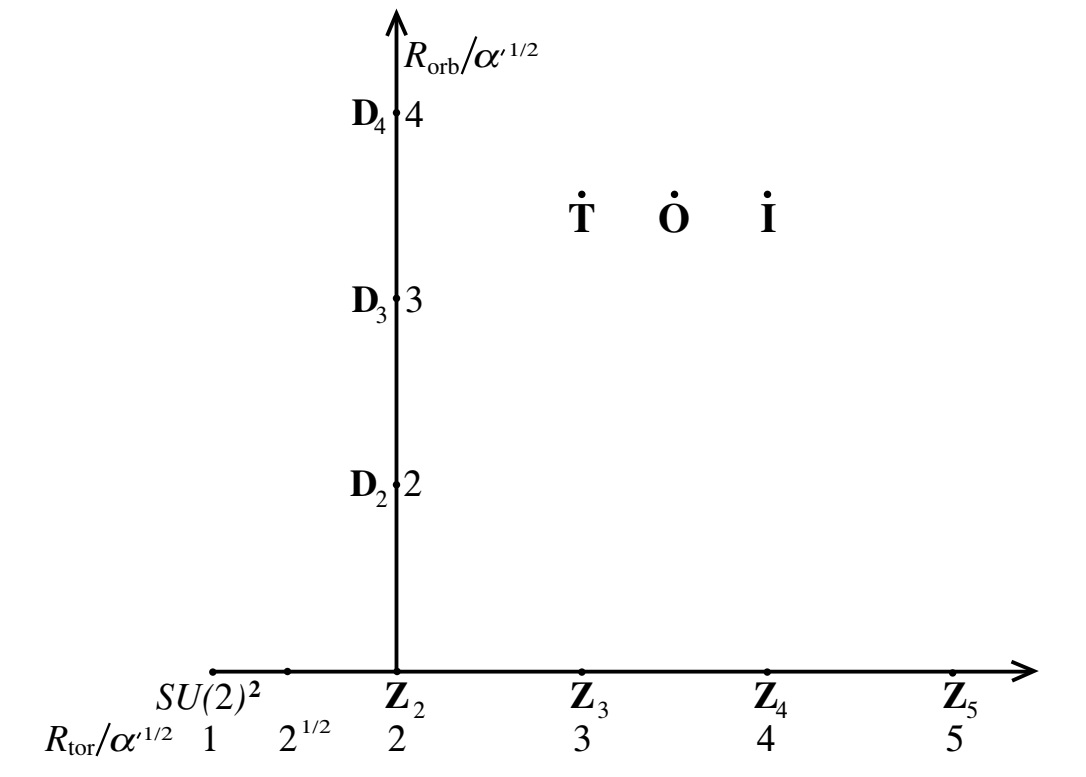
\includegraphics[width=0.8\textwidth,natwidth=814.5,natheight=582.75]{Fig8.2.jpg}
		\caption{$c=1$ CFT 的模空间. 水平轴是环向分支, 而垂直轴是轨形分支. 图中标出的点是用$SU(2)$群的一个离散子群扭曲获得的, 
		包含三个从四面体群, 八面体群和二十面体群获得的三个孤立点. 其它特殊半径, 诸如$R=(2 \alpha^{\prime})^{1/2}$处的环面, 后面会出现.}\label{Fig8.2}
	\end{center}
\end{figure}

这种等价性仅在这些半径处成立. 例如, 对于一般的$R$, 环向理论只有 $U(1) \times U(1)$规范对称性, 而轨形没有规范对称性. 
因此, 二者模空间的联系如图\ref{Fig8.2}所示. 有不同分支的模空间在特殊的点处会合, 在超对称理论中, 这一结构拥有非常普遍且重要的特征. 
一般而言, 在每一个分支会有不同的低能有效理论, 在这里的表现是低能规范对称性. 在特殊点的附近存在更多的轻场. 
随着我们沿着不同分支远离特殊点, 它们的不同子集会变得有质量.

环向分支与轨形分支交叉点附近的低能物理很有启发意义. 用\eqref{8.5.20}中的$r^{\prime}$扭曲的 $S U(2)$ 理论来描述它. 
在这一扭曲下留存的无质量标量是 $j^{3} \tilde{\jmath}^{3}$ 以及 $j^{i} \tilde{\jmath}^{j}$, 其中$i, j \in\{1,2\}$. 
既然它们是非扭的, 势与扭曲之前相同, 即 $\mathrm{det} M$. 标量场 $M_{i j}$依旧可以通过 $U(1) \times U(1)$ 旋转对角化, 
并且仅当一个对角元非零时, 势是平坦的. 然而, 现在模 $M_{33}$ 无法旋转至 $M_{11}$ 或 $M_{22}$, 所以这些方向在物理上不同. 
模$M_{33}$保持 $U(1) \times U(1)$ 不破坏, 并对应于沿着环向分支的移动. 模$M_{11}$ 或 $M_{22}$破缺了规范对称, 并对应于沿着轨形分支的移动. 
既然这个模是带荷的, 它的符号反转是规范变换, 所以物理上不同的轨形终于分支的交叉点. 我们无法同时变换两个模, 因为它们的线性组合不是平坦方向. 
轨形上的弦理论等价于圆上的弦理论, 这是相当可观的. 这表明弦看待时空几何的方式与我们并非完全相同.

沿着环向分支进行移动, 在 $SU(2)$半径的整数倍 $R=k \alpha^{\prime 1/2} $ 会有额外的无质量态. 这些态有 $(n, w)=(\pm 2 k, 0)$. 
我们可以认为这些点是这样获得的, 在$T$-对偶处理下,  $R=\alpha^{\prime 1/2} / k$,
 它们又是通过用$\mathds{Z}_{k}$对称性扭曲 $S U(2) \times S U(2)$理论得到
\begin{equation}
	X^{25} \rightarrow X^{25}+\frac{2 \pi \alpha^{\prime 1/2}}{k} \:. \label{8.5.22}
\end{equation}
这给 $j^{1}+\mi j^{2}$ 和 $\tilde{\jmath}^{1}+\mi \tilde{\jmath}^{2}$ 乘上了 $\exp (2 \pi \mi / k)$ , 因而幸存的无质量标量是
\begin{equation}
	j^{3} \tilde{\jmath}^{3}, \quad j^{1} \tilde{\jmath}^{1}+j^{2} \tilde{\jmath}^{2}, \quad 
	j^{1} \tilde{\jmath}^{2}-j^{2} \tilde{\jmath}^{1} \:. \label{8.5.23}
\end{equation}
这些中的第一个改变了环面的半径, 因而总是平坦方向. 然而, 因为在方向$M_{11}=M_{22}$ 或 $M_{12}=-M_{21}$上不会遇到势的平坦性条件\eqref{8.3.23}, 
从这些点中不再浮现其他分支.

偏移 \eqref{8.5.22} 生成了$S U(2) \times S U(2) $的$\mathds{Z}_{k}$子群. 我们来考察其他子群的扭曲. 
二面体群$\mathbf{D}_{k}$ 由偏移 \eqref{8.5.22} 和反射 $X^{25} \rightarrow-X^{25}$ 构成, 这给出了半径$k \alpha^{\prime 1/2}$处的轨形. 
其他三个离散子群是四面体群、八面体群以及二十面体群. 它们从CFT中移除了所有模, 所以扭曲CFT是孤立点, 不是连续族中的成员. 
不像 $\mathds{Z}_{k}$ 和 $\mathbf{D}_{k}$ 扭曲, 它们可以在所有半径处定义, 而这些包含 $S U(2)$元素的离散子群仅在离散半径处存在, 
因而半径不能在扭曲后变化. 有这种紧致化空间的弦论只会有一个标量——伸缩子. 

这是所有已知的 $c=1$的 CFT, 因而给出了所有已知的25维玻色弦背景.


\section{开弦} \label{sec:8.6}%{8.6 Open strings}

在开弦的环向紧致化中有一个新特征, 即有可能存在非平庸的威尔逊线, 规范场的平坦背景. 首先研究一些带有带荷场的$U(1)$规范理论, 考察常背景
\begin{equation}
	A_{25}(x^{M})=-\frac{\theta}{2 \pi R}=-\mi \Lambda^{-1} \frac{\partial \Lambda}{\partial x^{25}}, \quad 
	\Lambda(x^{25})=\exp \biggl(-\frac{\mi \theta x^{25}}{2 \pi R}\biggr) \:, \label{8.6.1}
\end{equation}
其中$\theta$是常数. 定域上看, 这是纯规范, 场强为零, 场方程是平庸的. 然而, 规范参量 $\Lambda$ 不满足时空周期性, 所以背景有物理效应. 
衡量这一效应的规范不变量是威尔逊线
\begin{equation}
	W_{q}=\exp \biggl(\mi q \oint \dif x^{25}\: A_{25}\biggr)=\exp (-\mi q \theta) \:. \label{8.6.2}
\end{equation}

首先考察电荷为$q$的点粒子, 它的规范固定作用量
\begin{equation}
	S=\int \dif \tau \: \biggl(\frac{1}{2} \dot{X}^{M} \dot{X}_{M}+\frac{m^{2}}{2}-\mi q A_{M} \dot{X}^{M}\biggr) \:. \label{8.6.3}
\end{equation}
规范作用量就是$-\mi q \int \dif x^{M}\, A_{M}$, 所以绕紧致维度一周的路径会挑出等于威尔逊线 $W_{q} $的相位. 正则动量是
\begin{equation}
	p_{25}=-\frac{\partial L}{\partial v^{25}}=v^{25}-\frac{q \theta}{2 \pi R} \:, \label{8.6.4}
\end{equation}
其中, 同\eqref{8.4.6}一样, $v^{25}=\mi \dot{X}^{25}$. 波函数在紧致维度中必须是周期的, 所以 $p_{25}=l/R$, $l$为整数, 并且
\begin{equation}
	v_{25}=\frac{2 \pi l+q \theta}{2 \pi R} \:. \label{8.6.5}
\end{equation}
湮灭物理态的哈密顿量是
\begin{equation}
	H=\frac{1}{2} (p_{\mu} p^{\mu}+v_{25}^{2}+m^{2}) \:, \label{8.6.6}
\end{equation}
由于 $v_{25}$ 依赖$\theta$, 所以 $-p_{\mu} p^{\mu}$ 发生了偏移. 相同的频谱可以在场描述下获得. 
注意, $v_{25}$ 正是规范不变动量$-\mi \partial_{25}-q A_{25}$.

我们也可做规范变换 $\Lambda^{-1}$令 $A_{25}$为零, 这一规范下带荷场不再是周期的, 
在$x^{25} \rightarrow x^{25}+2 \pi R$下挑出相位 $\exp (\mi q \theta)$. 物理量依旧是周期的. 正则动量现在偏移了, 我们有
\begin{equation}
	v_{25}=p_{25}=\frac{2 \pi l+q \theta}{2 \pi R}\:, \label{8.6.7}
\end{equation}
与之前一样, 对于规范不变动量 $v_{25}$获得了相同结果.

现在我们回到弦, 引入 $U(n)$ Chan-Paton 因子. 一般常数 $A_{25}$可以通过规范变换对角化
\begin{equation}
	A_{25}=-\frac{1}{2 \pi R} \operatorname{diag}(\theta_{1}, \theta_{2}, \ldots, \theta_{n}) \:. \label{8.6.8}
\end{equation}
这个规范场处在$U(n)$的对角群中, 即$U(1)^{n}$. 规范场与一般态的Chan-Paton因子的耦合为 $[A_{M}, \lambda]$, 
所以Chan-Paton 态 $|i j\rangle$ 中的弦在$U(1)_{i}$下有荷$+1$, 在$U(1)_{j}$下有荷$-1$, 在其他情况下为中性. 因此它有
\begin{equation}
	v_{25}=\frac{2 \pi l-\theta_{j}+\theta_{i}}{2 \pi R} \:. \label{8.6.9}
\end{equation}
那么开弦频谱就是
\begin{equation}
	m^{2}=\frac{(2 \pi l-\theta_{j}+\theta_{i})^{2}}{4 \pi^{2} R^{2}}+\frac{1}{\alpha^{\prime}}(N-1) \:. \label{8.6.10}
\end{equation}

考察规范玻色子, 这是 $l=0$ 且 $N=1$, 因此
\begin{equation}
	m^{2}=\frac{(\theta_{j}-\theta_{i})^{2}}{4 \pi^{2} R^{2}} \:. \label{8.6.11}
\end{equation}
在一般背景下, 所有 $\theta$都不同, 仅有的无质量矢量是对角的, $i=j$. 在这一情况下, 未破缺规范群是 $U(1)^{n} $. 
如果 $r$个 $\theta$ 相等, 相应的矢量的 $r \times r$矩阵是无质量的, 携带规范对称性$U(r)$. 将 $n$个 $\theta$分到集合 $r_{i}$中, 规范对称性是
\begin{equation}
	U(r_{1}) \times \ldots \times U(r_{s}), \quad \sum_{i=1}^{s} r_{i}=n \:. \label{8.6.12}
\end{equation}
像之前一样, 这有一个低能解释. 规范场$A_{25}$是 $U(n)$伴随表示中的25维标量, 而它的真空期望值将对称性破缺至$U(r_{1}) \times \ldots \times U(r_{s})$.

读者可以填补低能有效作用量的细节. 需要注意的是, 若紧致维度有$k$个, 势中会包含
\begin{equation}
	\operatorname{Tr}\Bigl([A_{m}, A_{n}]^{2}\Bigr) \:, \label{8.6.13}
\end{equation}
它来自26维Yang-Mills作用量中的场强. 这迫使不同方向的规范场在静态解中对易, 使得它们可同时对角化. 规范场中会给出$kn$个模, 
度规和反对称张量会给出 $k^{2}$ 个模.

\subsection*{$T$-对偶}

现在考察开弦频谱的 $R \rightarrow 0$ 极限. 若开弦的边界是 Neumann 边界, 它没有类似于 $w$ 的量子数; 它们总可以从紧致维上解开. 
所以, 当 $R \rightarrow 0$ 时, 动量不为零的态获得无限大质量, 但不再有新的连续态. 这与场论中的行为一致: 相应的态在25个时空维中移动.

我们知道有开弦的理论必有闭弦, 这貌似会产生矛盾. 这使得在 $R \rightarrow 0$的极限下, 闭弦在26个时空维中移动, 而开弦在25个时空维中移动. 
由此可推理出发生了如下事情: 开弦的内部与闭弦相同, 由同一“物质”构成, 所以依旧在26维振动. 区分开弦的正是它们的端点, 
所以它们必须限制在一个25维超平面上. 

事实确实如此, 我们可以用新的嵌入坐标来描述$T$-对偶理论
\begin{equation}
	X^{\prime 25}(z, \bar{z})=X_{L}^{25}(z)-X_{R}^{25}(\bar{z}) \:. \label{8.6.14}
\end{equation}
那么
\begin{equation}
	\partial_{n} X^{25}=-\mi \partial_{t} X^{\prime 25} \:, \label{8.6.15}
\end{equation}
其中 $n$是边界的法向,  $t$是边界的切向. 原始坐标上的 Neumann 边界就是对偶坐标上的 Dirichlet 边界: 每个弦端点的$X^{\prime 25}$坐标是固定的. 

我们先来考察没有威尔逊线的紧致化. 那么所有端点都约束在同一超平面上. 为看到这一点, 积分
\begin{align}
		X^{\prime 25}(\pi)-X^{\prime 25}(0) &= \int_{0}^{\pi} \dif \sigma^{1}\: \partial_{1} X^{\prime 25}
											 = -\mi \int_{0}^{\pi} \dif \sigma^{1}\: \partial_{2} X^{25} \nonumber \\
											&= -2 \pi \alpha^{\prime} v^{25}
											 = -\frac{2 \pi \alpha^{\prime} l}{R}=-2 \pi l R^{\prime} \:. \label{8.6.16}
\end{align}
$X^{\prime 25}$在两个端点之间的总变化是对偶维周期$2 \pi R^{\prime}$的整数倍, 所以末端处在周期$T$对偶空间的同一超平面上. 
对于两个不同的开弦, 它们之间交换引力子会给出连通世界面. 我们可以对此进行与\eqref{8.6.16}相同的讨论, 所以, 所有弦的端点都处在同一超平面上, 
见图\ref{Fig8.3}. 端点在其他24维依旧是随意移动的.

\begin{figure}[h]
	\begin{center}
		%width=0.8\textwidth,bb=0 0 761 723
		%1px=0.75pt
		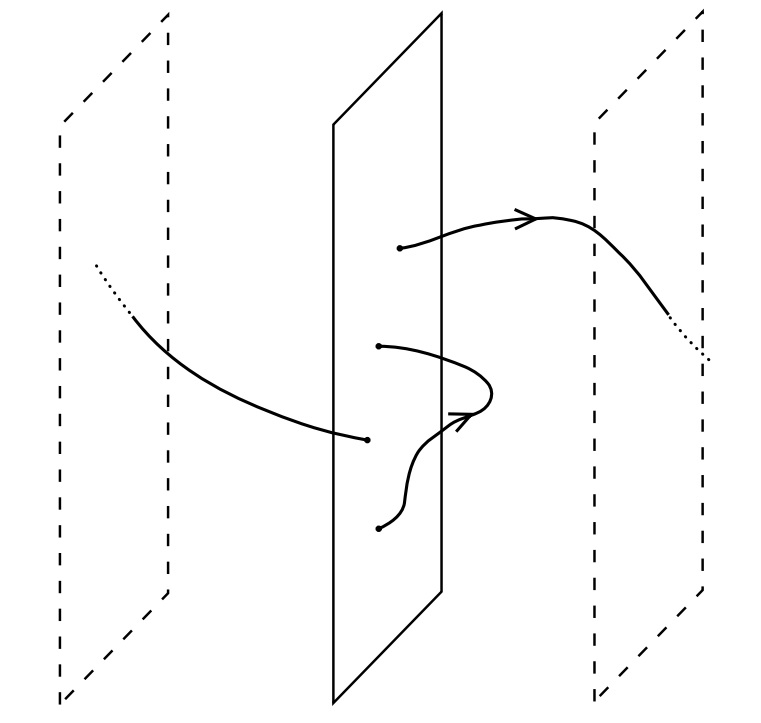
\includegraphics[width=0.7\textwidth,natwidth=532.7,natheight=530]{Fig8.3.jpg}
		\caption{端点连在超平面上的开弦. 虚线标出的平面是周期等价的平面. 图中展示出了两条弦, 缠绕数分别为1和0.}\label{Fig8.3}
	\end{center}
\end{figure}

现在我们来看威尔逊线的效应. 由于$v_{25}$中有偏移\eqref{8.6.9}, \eqref{8.6.16}被换成
\begin{equation}
	\Delta X^{\prime 25}=X^{\prime 25}(\pi)-X^{\prime 25}(0)=-(2 \pi l-\theta_{j}+\theta_{i}) R^{\prime} \:. \label{8.6.17}
\end{equation}
换句话说, 除去一个额外的归一化,  $i$ 态上的端点处在
\begin{equation}
	X^{\prime 25}=\theta_{i} R^{\prime}=-2 \pi \alpha^{\prime} A_{25, i i} \:. \label{8.6.18}
\end{equation}
因此, 一般会有$n$个不同的超平面, 见图\ref{Fig8.4}.

\begin{figure}[h!]
	\begin{center}
		%width=0.8\textwidth,bb=0 0 938 756
		%1px=0.75pt
		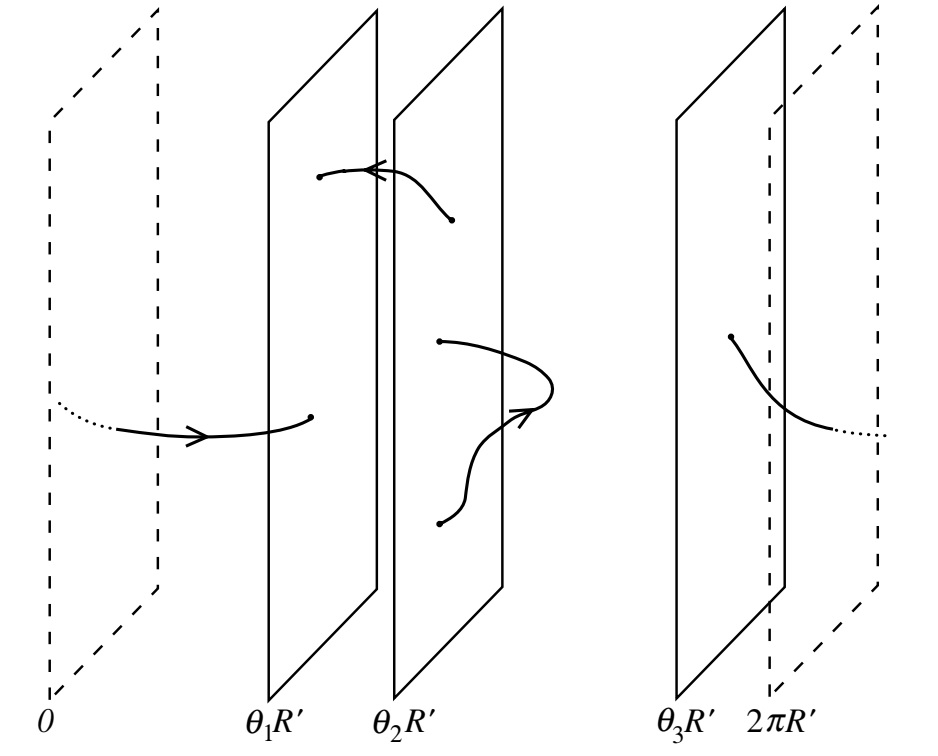
\includegraphics[width=0.8\textwidth,natwidth=656.6,natheight=555]{Fig8.4.jpg}
		\caption{处在不同位置的$n=3$个超平面, 上面连上了不同的弦. 忽略快子, 两端连在同一超平面的最轻弦是无质量的, 而连接两个不重合的超平面的弦由于张力是有质量的. 当两个超平面重合时, 连接超平面的最轻弦变成无质量的.}\label{Fig8.4}
	\end{center}
\end{figure}

我们来考察Chan-Paton态 $|i j\rangle$的模式展开, 并假定它在紧致维数上缠绕了$l$次
\begin{align}
	X^{\prime 25}(z, \bar{z}) &= \theta_{i} R^{\prime} - \frac{\mi R^{\prime}}{2 \pi}(2 \pi l-\theta_{j}+\theta_{i}) 
	\ln (z / \bar{z}) + \mi \biggl(\frac{\alpha^{\prime}}{2}\biggr)^{1/2} 
	\sum_{\substack{m=-\infty  \\  m \neq 0}}^{\infty} \frac{\alpha_{m}^{25}}{m}(z^{-m}-\bar{z}^{-m})  \nonumber \\
	&=\theta_{i} R^{\prime} + \frac{\sigma^{1}}{\pi} \Delta X^{\prime 25} - (2 \alpha^{\prime})^{1/2} 
	\sum_{\substack{m=-\infty  \\  m \neq 0}}^{\infty} \frac{\alpha_{m}^{25}}{m} \exp (-m \sigma^{2}) \sin m \sigma^{1} \:. \label{8.6.19}
\end{align}
频谱 \eqref{8.6.10} 变成
\begin{equation}
	m^{2}=\biggl(\frac{\Delta X^{\prime 25}}{2 \pi \alpha^{\prime}}\biggr)^{2}+\frac{1}{\alpha^{\prime}}(N-1) \:, \label{8.6.20}
\end{equation}
其中 $\Delta X^{\prime 25}$由\eqref{8.6.17}给定. 它是弦在给定分区中的最短长度.

现在来考察, 如果有多个紧致维, 这个图景怎么推广. 设 $X^{m}$是周期维, 其中 $p+1 \leq m \leq 25$. 我们将周期维写成对偶坐标的形式. 
$X^{m}$上的 Neumann 条件又一次变成对偶坐标 $X^{\prime m}$上的 Dirichlet 条件, 所以开弦端点拘束在$n$ 个平行的$(p+1)$-维子空间中. 
对于每个子空间, 不同方向的威尔逊线变成独立坐标.

由于平移不变性被开弦边界条件破坏了, 对偶背景相当古怪. 这反映了如下事实: 在原始开弦理论中, 缠绕数不守恒, 而缠绕数$T$对偶到动量. 
$T$对偶只是同一理论的不同描述. 更进一步, 当紧致半径很小时, 那么就应该自然地使用$T$对偶图景.

\section{D膜}%{8.7 D-branes}
我们现在知道, 当开弦理论紧致化在一个小环面上时, 它的物理可以描述成在大环面上的紧致化, 但是开弦的端点约束在子空间中. 事实上, 这些子空间本身是新的动力学客体.

在一般构形下考虑无质量开弦的频谱, 在这种构形下, 所有$\theta_{i}$都不同, 简单起见, 只取一个坐标是对偶化的. 
忽视快子, 质量\eqref{8.6.20}仅在$N=1$且 $\Delta X^{\prime 25}=0 $ 时为零. 即, 两个端点处在同一超平面且缠绕数为零. 因而我们有无质量态
\begin{subequations} \label{8.7.1}
\begin{align}
	&\alpha_{-1}^{\mu}|k; ii\rangle \:, \quad \mathscr{V} = \mi \partial_{t} X^{\mu}  \:, \label{8.7.1a} \\
	&\alpha_{-1}^{25} |k; ii\rangle \:, \quad \mathscr{V} = \mi \partial_{t} X^{25} = \partial_{n} X^{\prime 25} \:. \label{8.7.1b}
\end{align}
\end{subequations}
它们显然就是原始理论中的无质量态, $T$-对偶只是给了同一频谱的不同图景. 对于一般的威尔逊线, 唯一的无质量开弦态将是$n$个无质量$U(1)$矢量. 
在\eqref{8.7.1}中, 我们根据它们是切于超平面还是垂直于超平面将其分类. 有切向极化的25个态构成了处在超平面上的规范场, 
而它在$T$-对偶理论中有一个简单且重要的解释: 它是超平面形状的坐标集. 从常数规范场\eqref{8.6.18}对应于超平面的均匀平移就可以看到这一点. 
依赖$x^{\mu}$的背景可以转至一个依赖$x^{\mu}$的平移, 一个弯曲的超平面, 而场 $A_{ii}^{25}$ 的量子对应超平面的微小振荡.

这与时空上发生的现象相同. 我们从平坦背景中的弦出发, 发现无质量闭弦态对应几何的涨落. 
在这里, 我们首先发现超平面, 然后发现特定的开弦态对应于超平面的涨落. 我们不应该对超平面有动力学感到惊讶. 
弦论包含引力. 引力波穿越超平面时将会扰动时空本身, 所以超平面很难保持刚性.

因此, 超平面确实是动力学客体, 这是D膜. 对于$25-p$个维度做对偶会得到p维膜, 称为 D$p$-膜. 
利用这个术语, 原始的 $U(n)$ 开弦理论会包含 $n$个 D25-膜. D25-膜填满了空间, 所以弦端点没有约束: 它仅对应一般的 Chan-Paton 因子.

既然$T$ 对偶交换了Neumann与Dirichlet边界条件, 在与D$p$膜相切的方向上做$T$对偶会将其约化至 D$(p{-}1)$-膜, 
而在垂直方向上做 $T$ 对偶则将其约化至D$(p{+}1)$-膜. 非平庸角的情况也会立刻出现. 

我们本可以通过研究Dirichlet边界本身出发. 这里我们所采取的路线是从$T$对偶发现它们, 这一方法能更好的发展它们的性质. 
也可证明, 通过一个连续的过程, 我们能从``普通''态到达包含D-膜的态. 即, 取普通理论的$R \rightarrow 0$极限, 这使得非紧致空间中有$n$个D-膜. 
在超弦中, 我们将用这一点来论证D-膜是理论的非微扰定义中的重要部分. 对于玻色弦, 由于没有很强的证据表明它有非微扰定义, 我们不做这个讨论. 
玻色弦论有可能仅是作为超弦的部分而存在.

我们来看一下$T$对偶图景中的$U(n)$对称性破缺. 当没有D-膜重合时, 仅在每个D-膜上有无质量矢量, 这给出规范群 $U(1)^{n}$. 
如果有$r$个D-膜重合, 那么会有额外的无质量态, 连接这些膜的弦长为零: 当$n=0$时, 若 $i$ 与$j$均在集合$r$中, 
质量公式\eqref{8.6.20}中的 $\Delta X^{\prime 25}$为零. 因此, 存在$r^{2}$ 个矢量, 构成$U(r)$规范群的伴随表示. 
这与对偶威尔逊线图景中发现的相同. 然而, 令人惊奇的是, 在垂直D-膜的方向上会有$r^{2}$个无质量标量. 我们会在下面讨论它的意义.

\subsection*{D-膜作用量}
在D$p$-膜的世界体上, 无质量场是$U(1)$矢量和描述涨落的 $25{-}p$ 世界膜标量. 这个系统的低能有效作用量总是值得考察的. 
我们取对偶半径$R^{\prime}$为无穷, 只考虑相应26维时空中的单个D膜. 世界膜场与无质量闭弦场有相互作用, 而它的作用量在\ref{sec:3.7}节讨论过. 
引入膜上的坐标 $\xi^{a}$, 其中$a=0, \ldots p$. 膜上的场是嵌入 $X^{\mu}(\xi)$ 以及规范场$A_{a}(\xi)$. 我们声明作用量
\begin{equation}
	\bm{S}_{p} = -T_{p} \int \dif^{p+1} \xi \: 
				\me^{-\Phi}[-\operatorname{det}(G_{ab} + B_{ab} + 2 \pi \alpha^{\prime} F_{a b})]^{1/2} \:, \label{8.7.2}
\end{equation}
其中$T_{p}$是待定常数. 这里
\begin{equation}
	G_{ab}(\xi) = \frac{\partial X^{\mu}}{\partial \xi^{a}} \frac{\partial X^{\nu}}{\partial \xi^{b}} G_{\mu \nu}(X(\xi)), \quad 
	B_{ab}(\xi) = \frac{\partial X^{\mu}}{\partial \xi^{a}} \frac{\partial X^{\nu}}{\partial \xi^{b}} B_{\mu \nu}(X(\xi)) \label{8.7.3}
\end{equation}
是膜上的诱导度规以及诱导反对称张量.

基于一般推理就可以理解\eqref{8.7.2}的所有特征. 首先, 只考察时空度规以及嵌入, 
最简单且导数最少的坐标无关作用量是 $(-\operatorname{det} G_{a b})^{1/2}$的积分, 即世界体积. 
注意到, 这一项经由诱导场\eqref{8.7.3}对$X^{\mu}(\xi)$有隐式关系. 围绕一个平坦D-膜做展开, 这给出涨落的作用量, 
就像Nambu-Goto作用量作用量描述了弦的涨落.

出现对伸缩子的依赖 $\me^{-\Phi} \propto g_{\mathrm{c}}^{-1}$ 是因为这是开弦树图作用量. 
开弦场的自相互作用, 以及它们与闭弦场的耦合, 最初来自于圆盘.

对 $F_{ab}$ 的依赖性可以通过$T$-对偶理解. 考察沿 $X^{1}$ 和 $X^{2}$ 方向铺展的D膜, 其他方向未指定, 并令上面有一个常数规范场 $F_{12}$. 
去往规范 $A_{2}=X^{1} F_{12}$. 现在沿$X^{2}$方向取$T$-对偶. 在这一方向的Neumann条件就变成了Dirichlet条件, 所以, D膜少了一个维数. 
然而, 势与坐标之间的关系\eqref{8.6.18}暗示了D-膜在 (1-2)-平面中是倾斜的
\begin{equation}
	X^{\prime 2}=-2 \pi \alpha^{\prime} X^{1} F_{12} \:. \label{8.7.4}
\end{equation}
这个倾斜赋予了作用量一个几何因子
\begin{equation}
	 \int \dif X^{1}\: \Bigl[1 + (\partial_{1} X^{\prime 2})^{2}\Bigr]^{1/2} 
	=\int \dif X^{1}\: \Bigl[1 + (2 \pi \alpha^{\prime} F_{12})^{2}\Bigr]^{1/2} \:. \label{8.7.5}
\end{equation}
对任意D-膜, 通过推动使其与坐标轴对齐, 并进行旋转, 使 $F_{ab}$ 变成对角形式, 可以将作用量约化至每一平面中的因子\eqref{8.7.5}的积, 
等价于行列式中的 $F_{ab}$ 项. 规范场构成的行列式称为Born-Infeld作用量, 它最初是为了解决量子电动力学的短程发散问题.

最后, 对 $B_{ab}$ 的依赖关系由如下讨论给出. 在弦的世界面作用量中, 闭弦场$B_{\mu \nu}$与开弦场$A^{\mu}$以如下形式出现
\footnote{对于熟悉微分形式的读者, 这是
	\[ \frac{\mi}{2 \pi \alpha^{\prime}} \int_{M} B + \mi \int_{\partial M} A \:. \]
后面的方程可以用类似的方式翻译.}
\begin{equation}
	\frac{\mi}{4 \pi \alpha^{\prime}} \int_{M} \dif^{2} \sigma \: g^{1/2} \epsilon^{ab} \partial_{a} X^{\mu} \partial_{b} X^{\nu} 
	B_{\mu\nu} + \mi \int_{\partial M} \dif X^{\mu} \:A_{\mu} \:. \label{8.7.6}
\end{equation}
这些场中的每一个都会附带一个时空规范不变性, 为了与时空理论相容必须予以保留. 通常的规范变换
\begin{equation}
	\delta A_{\mu}=\partial_{\mu} \lambda \label{8.7.7}
\end{equation}
是作用量\eqref{8.7.6}的一个不变性, 边界项会差一个全导数的积分. 反对称张量变分
\begin{equation}
	\delta B_{\mu \nu} = \partial_{\mu} \zeta_{\nu} - \partial_{\nu} \zeta_{\mu} \label{8.7.8}
\end{equation}
会使得``块''作用量差一个全导数, 但在有边界的世界面上, 这给出表面项. 要使得它抵消, 在张量规范对称性, 开弦场 $A_{\mu}$ 要有变换
\begin{equation}
	\delta A_{\mu}=-\zeta_{\mu} / 2 \pi \alpha^{\prime} \:. \label{8.7.9}
\end{equation}
现在, 只有组合
\begin{equation}
	B_{\mu \nu}+2 \pi \alpha^{\prime} F_{\mu \nu} \equiv 2 \pi \alpha^{\prime} \mathscr{F}_{\mu \nu}  \label{8.7.10}
\end{equation}
在两个对称性下是不变的, 因此出现在作用量中的必须是这个组合. 因此, 作用量的形式\eqref{8.7.2}就完全确定了.

作为检验, 由于相同的组合出现在共形规范下的世界面作用量中, 很自然地, 组合 $G_{\mu \nu}+B_{\mu \nu}$ 应该出现. 
也可以取各种开弦振幅以及开弦-闭弦振幅的低能极限来决定作用量\eqref{8.7.2}, 但这会费劲得多.

对于$n$个分立的D-膜, 作用量是$n$份儿单个D-膜作用量. 然而, 我们已经看到, 当D-膜重合时, 膜上会有 $n^{2}$ 个, 而不是 $n$个无质量矢量和标量, 
我们将写下这一情况的有效作用量. 场 $X^{\mu}(\xi)$以及 $A_{a}(\xi)$ 现在将是 $n \times n$ 矩阵. 对于规范场, 
含义是显然的——它变成了非阿贝尔 $U(n)$ 规范场. 然而, 对于坐标集 $X^{\mu}$, 含义是不清楚的: $n$ 个D-膜到时空的嵌入坐标集扩展成 $n \times n$ 矩阵. 
已经证明, 非对易几何在D-膜的动力学中扮演了重要角色, 这里有一个猜想: 它是时空特性的一个重要线索.

通过考察有效作用量, 我们可以获得更多启发. 作用量中现在有了非导数项, 它是坐标集的势, 这可以从常数 $A_{m}$ 场的 $T$-对偶中推断出来. 
对于这样的矢量势, 场强就是$[A_{m}, A_{n}]$, 它在$T$-对偶图景中变成了$(2 \pi \alpha^{\prime})^{-2}[X_{m}, X_{n}]$. 
在场强中展开, 作用量的领头阶大约是
\begin{equation}
	V \propto \operatorname{Tr}([X_{m}, X_{n}][X^{m}, X^{n}]) \:. \label{8.7.11}
\end{equation}
这个势在$X^{m}=0$处的二阶导数为零, 这使得所有$k n^{2}$个标量均无质量; 同以往一样 $k=25{-}p$ 是对偶维数. 
然而平坦维数的空间更小些. 势是平方和, 所以只在所有 $[X^{m}, X^{n}]$为零时为零. 我们可以用 $U(n)$对称性去往 $X^{m}$ 都对角的规范. 
因此会有 $kn$ 个平坦方向, 正是对角元个数. 这样, $kn$ 个对角元可以解释成 $n$ 个D$p$-膜坐标集. 
因此\eqref{8.7.11}正确地介入了分离D-膜与重合D-膜的物理.

当 $X^{m}$ 对易时, 作用量应该退化到$n$个分立的D-膜, 所以有
\begin{align}
	\bm{S}_{p} &= -T_{p} \int \dif^{p+1} \xi \: \operatorname{Tr} \Bigl\{ \me^{-\Phi}
	              [-\operatorname{det}(G_{ab} + B_{ab} + 2 \pi \alpha^{\prime} F_{ab})]^{1/2} \nonumber \\
		       &\qquad \qquad \qquad \quad + O([X^{m}, X^{n}]^{2})\Bigr\} \:. \label{8.7.12}
\end{align}
行列式取在世界体指标 $ab$上, 迹取在 $n$个 Chan-Paton指标上. 迹是合适的 $U(n)$ 不变量, 对于对角矩阵, 它退化成对分离D-膜的求和. 
对对易子的完整依赖关系要比简单的势 \eqref{8.7.11} 复杂得多, 其中会包含与其他场的耦合, 以及对易子的高阶修正. 
然而, 关键性质, 平坦方向的形式是不受影响的. 通过从完全Neumann情况下的 Born-Infeld 作用量出发, 并进行$T$-对偶, 我们可得到完全的依赖性. 
附带地, 包含场强对易子的高阶导数项不能仅用 $T$ 对偶就决定下来.

\subsection*{D-膜张力}
计算常数$T_{p}$是很有意义的, 并且对于超弦, 它的精确值非常重要. 在进行显式的计算之前, 注意到从$T$对偶可得到 $T_{p}$ 的递推关系. 
注意到, 在常数伸缩子背景下, D$p$-膜的张力是 $T_{p} \me^{-\Phi}$: 这是静态D$p$-膜单位体积内作用量的相反数. 
现在考察这样的D$p$-膜, 与该D$p$膜相切的 $p$ 个方向周期等价. 即, D$p$-膜绕在时空中的一个$p$-环面上. 它的质量是它的张力乘以它的环面的面积
\begin{equation}
	T_{p} \me^{-\Phi} \prod_{i=1}^{p}(2 \pi R_{i}) \:. \label{8.7.13}
\end{equation}
现在, 对其中一个周期方向$X^{p}$取$T$对偶. 这样不改变质量, 只是同样一个态的新描述. 用$T$-对偶理论的伸缩子\eqref{8.3.31}, 质量\eqref{8.7.13}是
\begin{equation}
	2 \pi \alpha^{\prime 1/2} T_{p} \me^{-\Phi^{\prime}} \prod_{i=1}^{p-1}(2 \pi R_{i}) \:. \label{8.7.14}
\end{equation}
\begin{tcolorbox}
	\begin{remark}
		利用了$\sqrt{\alpha^\prime}\me^{-\Phi^\prime}/R_p=\me^{-\Phi}$	
	\end{remark}	
\end{tcolorbox}
\noindent 然而, 在对偶理论中, 这相当于是 $\mathrm{D}(p{-}1)$-膜缠绕在$(p{-}1)$-环面上, 所以它的质量是
\begin{equation}
	T_{p-1} \me^{-\Phi^{\prime}} \prod_{i=1}^{p-1}(2 \pi R_{i}) \:. \label{8.7.15}
\end{equation}
联立 \eqref{8.7.14} 和 \eqref{8.7.15} 给出
\begin{equation}
	T_{p}=T_{p-1} / 2 \pi \alpha^{\prime 1/2} \:, \label{8.7.16}
\end{equation}
除了一个总的归一化外, 这完全决定了$T_{p}$.

为了决定D-膜张力的实际值, 我们需要计算弦振幅. 例如, 我们可以从D-膜的引力耦合将其推断出来, 这个振幅由一个带有引力子顶点算符的圆盘给出. 
然而, 这包含一个未知的比值 $g_{\mathrm{c}} / g_{\mathrm{o}}^{2}$, 闭弦耦合来自于顶点算符, 而开弦耦合源于圆盘. 
我们可以用另一方法获得绝对归一化. 考察两个平行的D$p$-膜, 它们分别在 $X_{1}^{m}=0$ 和 $X_{2}^{m}=y^{m}$ 处. 
通过交换闭弦, 这二者可以感到彼此的存在, 如图\ref{Fig8.5}所示. 弦振幅是圆环, 没有顶角算符, 可以用上一章的方法计算出来. 
那么, 交换引力子和伸缩子给出的极点, 就给出了闭弦态与D-膜的耦合$T_{p}$.
\begin{figure}
	\begin{center}
		%width=0.8\textwidth,bb=0 0 609 717
		%1px=0.75pt
		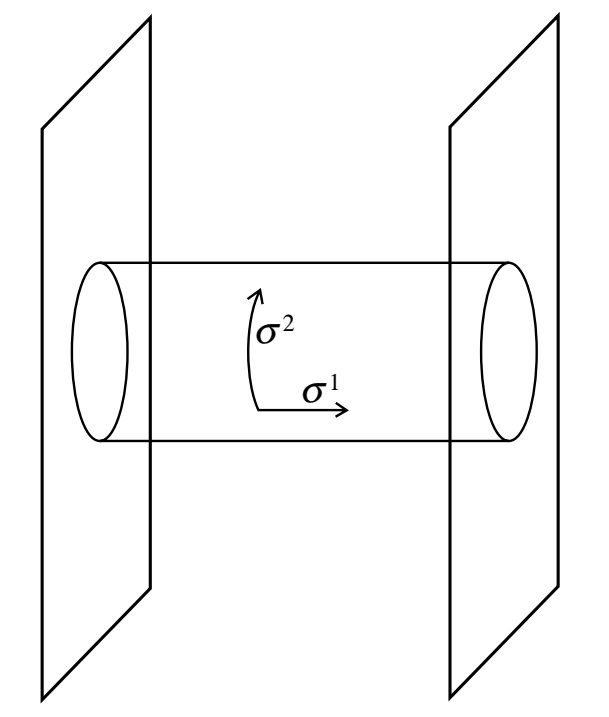
\includegraphics[width=0.6\textwidth,natwidth=426.3,natheight=520]{Fig8.5.jpg}\\
		\caption{在两个D-膜之间交换一个闭弦. 等价地, 这是端点连在两个D-膜的开弦的真空圈.}\label{Fig8.5}
	\end{center}
\end{figure}


在\ref{sec:7.4}节中, 我们用开弦圈计算了圆环真空振幅, 但从模积分的 $t \rightarrow 0$ 极限中发现了闭弦极点. 
这正是我们感兴趣的极点, 但计算振幅的最简单方法是视其为开弦圈. 事实上, 只要稍许改变, 就能用之前的结果\eqref{7.4.1}. 
动量积分的数目从26减少到$p{+}1$, 类似地, $V_{26}$ 变成 $V_{p+1}$; 权重 $h_{i}$ 由于拉伸开弦获得额外项 $y^{2} / 4\pi^{2} \alpha^{\prime}$; 
Chan-Paton 权重 $n^{2}$ 变成2(因为弦连接的方向有两个). 因此有
\begin{align}
	\mathscr{A} &= \mi V_{p+1} \int_{0}^{\infty} \frac{\dif t}{t} (8 \pi^{2} \alpha^{\prime} t)^{-(p+1)/2} 
				   \exp (-t y^{2} / 2 \pi \alpha^{\prime}) \eta(\mi t)^{-24}  \nonumber \\
				&= \frac{\mi V_{p+1}}{(8 \pi^{2} \alpha^{\prime})^{(p+1)/2}} 
				   \int_{0}^{\infty} \dif t\: t^{(21-p)/2} \exp (-t y^{2} / 2 \pi \alpha^{\prime}) \nonumber \\
				& \qquad \qquad \qquad \qquad \qquad  \times[\exp (2 \pi/t)+24+\cdots] \:, \label{8.7.17}
\end{align}
其中渐近展开以\ref{sec:7.4}节方法获得. 第一项是快子交换, 所以是玻色人工产物. 对第二项积分给出
\begin{align}
	\mathscr{A} &= \mi V_{p+1} \frac{24}{2^{12}}(4 \pi^{2} \alpha^{\prime})^{11-p} \pi^{(p-23)/2} 
				   \Gamma\biggl(\frac{23-p}{2}\biggr)|y|^{p-23}  \nonumber \\
				&= \mi V_{p+1} \frac{24 \pi}{2^{10}}(4 \pi^{2} \alpha^{\prime})^{11-p} G_{25-p}(y) \:, \label{8.7.18}
\end{align}
其中 $G_{d}(y)$ 是$d$ 维中无质量标量的格林函数, $-\nabla^{2}$的逆.

我们现在要与相同振幅的场论计算作一比较. 既然反对称张量不与D-膜耦合, 从时空作用量\eqref{3.7.25}中, 相关项是
\begin{equation}
	\bm{S}=\frac{1}{2 \kappa^{2}} \int \dif^{26} X \: (-\tilde{G})^{1/2} 
		   \biggl(\tilde{\bm{R}}-\frac{1}{6} \nabla_{\mu} \tilde{\Phi} \tilde{\nabla}^{\mu} \tilde{\Phi}\biggr) \:. \label{8.7.19}
\end{equation}
加波浪线是指爱因斯坦度规; 由于这一形式的作用量与伸缩子退耦, 所以比较方便. 加波浪线的伸缩子已经进行了偏移, 使得它的真空期望值为零. 
以同一变量的形式, D-膜作用量\eqref{8.7.2}中的相关项是
\begin{equation}
	\bm{S}_{p} = -\tau_{p} \int \dif^{p+1} \xi \: \exp \biggl(\frac{p-11}{12} \tilde{\Phi}\biggr)
				 (-\operatorname{det} \tilde{G}_{ab})^{1/2} \:. \label{8.7.20}
\end{equation}
我们定义了 $\tau_{p}=T_{p} \me^{-\Phi_{0}}$; 当伸缩子的背景值是$\Phi_{0}$时, 这是D$p$-膜的真实物理张力.

类比图\ref{Fig8.5}的场论图是在D-膜之间交换伸缩子或引力子. 为了获得传播子, 
我们将时空作用量展至$h_{\mu\nu}=\tilde{G}_{\mu\nu}-\eta_{\mu\nu}$ 和 $\tilde{\Phi}$的二阶. 
另外, 对于引力计算, 我们需要选择规范. 对于微扰计算, 最简单的规范是
\begin{equation}
	F_{\nu} \equiv \partial^{\hat{\mu}} h_{\mu \nu}-\frac{1}{2} \partial_{\nu} h^{\hat{\mu}}{}_{\mu}=0 \:, \label{8.7.21}
\end{equation}
其中, 加``帽子''是指用平坦度规 $\eta^{\mu \nu}$ 升降指标. 将作用量展开至二阶, 并加上规范固定项 $-F_{\nu} F^{\hat{\nu}} / 4\kappa^{2}$, 
时空作用量变成
\begin{equation}
	\bm{S}=-\frac{1}{8 \kappa^{2}} \int \dif^{26} X \: \biggl( \partial_{\mu} h_{\nu \lambda} 
	\partial^{\hat{\mu}} h^{\hat{\nu} \hat{\lambda}}-\frac{1}{2} \partial_{\mu} h^{\hat{\nu}}{}_{\nu} 
	\partial^{\hat{\mu}} h^{\hat{\lambda}}{}_{\lambda}+\frac{2}{3} \partial_{\mu} \tilde{\Phi} \partial^{\hat{\mu}} \tilde{\Phi}\biggr) \:. \label{8.7.22}
\end{equation}
观察动能项, 由此获得动量空间传播子
\begin{subequations} \label{8.7.23}
\begin{align}
		\langle\tilde{\Phi} \tilde{\Phi}\rangle &=-\frac{(D-2) \mi \kappa^{2}}{4 k^{2}}  \:, \label{8.7.23a} \\
		\langle h_{\mu \nu} h_{\sigma \rho}\rangle &=-\frac{2 \mi \kappa^{2}}{k^{2}}
		\biggl(\eta_{\mu \sigma} \eta_{\nu \rho}+\eta_{\mu \rho} \eta_{\nu \sigma}-\frac{2}{D-2} \eta_{\mu \nu} \eta_{\sigma \rho}\biggr) \:. \label{8.7.23b}
\end{align}
\end{subequations}
为了之后参考, 我们给出了一般的$D$. 围绕一般平坦构形展开, D-膜作用量是
\begin{equation}
	\bm{S}_{p}=-\tau_{p} \int \dif^{p+1} \xi \: \biggl(\frac{p-11}{12} \tilde{\Phi}-\frac{1}{2} h_{aa}\biggr) \:. \label{8.7.24}
\end{equation}
注意这里的$h_{\mu \nu}$ 仅对与D-膜相切的方向求迹; 我们已经取 $\xi$ 为度规为$\delta_{ab}$的直角坐标.

我们现在可读出费曼图
\begin{align}
	\mathscr{A} &= \frac{\mi \kappa^{2} \tau_{p}^{2}}{k_{\perp}^{2}} V_{p+1} 
				   \left\{6\left[\frac{p-11}{12}\right]^{2}+\frac{1}{2}\left[2(p+1)-\frac{1}{12}(p+1)^{2}\right]\right\} \nonumber \\
			    & =\frac{6 \mi \kappa^{2} \tau_{p}^{2}}{k_{\perp}^{2}} V_{p+1} \:. \label{8.7.25}
\end{align}
\begin{tcolorbox}
	\begin{remark}
		上式来自于$\langle S_p S_p \rangle$.
	\end{remark}	
\end{tcolorbox}
\noindent 与\eqref{8.7.18}比较给出
\begin{equation}
	\tau_{p}^{2} = \frac{\pi}{256 \kappa^{2}} (4 \pi^{2} \alpha^{\prime})^{11-p} \:. \label{8.7.26}
\end{equation}
这与$T$-对偶给出的递推关系一致.

作为一个应用, 考察有 $n$个25-膜的态, 这与普通的$n$值Chan-Paton 因子相同. 将25-膜作用量\eqref{8.7.12}展至规范场的二阶, 给出
\begin{equation}
	\frac{\tau_{25}}{4}(2 \pi \alpha^{\prime})^{2} \operatorname{Tr}(F_{\mu \nu} F^{\mu \nu}) \:. \label{8.7.27}
\end{equation}
这关联了开弦规范耦合与闭弦引力耦合. 利用\eqref{6.5.14}, \eqref{6.5.16}, \eqref{6.6.15}, 和 \eqref{6.6.18}, 
我们可以将其写为顶点算符归一化 $g_{\mathrm{c}}$ 与 $g_{\mathrm{o}}$之间的关系
\begin{equation}
	\frac{g_{\mathrm{o}}^{2}}{g_{\mathrm{c}}} = \frac{4 \pi \alpha^{\prime} g_{\mathrm{o}}^{\prime 2}}{\kappa}
											  = 2^{18} \pi^{25 / 2} \alpha^{\prime 6} \:. \label{8.7.28}
\end{equation}
它拥有正确的形式, 开弦耦合的平方正比于闭弦耦合, 但现在有了数值系数. 我们经由幺正性, 从圆环中分解出闭弦极点, 或参看习题7.9


\section{非定向弦的$T$-对偶} \label{sec:8.8}%{8.8 T-duality of unoriented theories}
在非定向的弦理论中,  $R \rightarrow 0$的极限也会给出有趣的新物理. 首先考察闭弦理论. 为了构成非定向理论, 我们在态上强加$\Omega=+1$. 
沿用\ref{sec:8.5}节的讨论, 我们也可认为这是规范化 $\Omega$. 特别地, 用来构建世界面的跃迁函数现在会反转方向, 并且这产生了非定向世界面.

$T$-对偶理论是通过用坐标$X^{\prime m}(z, \bar{z})= X_{L}^{m}(z)-X_{R}^{m}(\bar{z})$ 替换 
$X^{m}(z, \bar{z})=X_{L}^{m}(z)+X_{R}^{m}(\bar{z})$获得的. 在原始描述中, 我们规范化世界面宇称 $\Omega$, 它的作用
\begin{equation}
	\Omega: X_{L}^{M}(z) \leftrightarrow X_{R}^{M}(z) \:. \label{8.8.1}
\end{equation}
以$T$-对偶坐标, 这是
\begin{subequations} \label{8.8.2}
	\begin{align}
		\Omega: \quad X^{\prime m}(z, \bar{z})  &\leftrightarrow-X^{\prime m}(\bar{z}, z) \:, \label{8.8.2a} \\
		X^{\mu}(z, \bar{z})  &\leftrightarrow X^{\mu}(\bar{z}, z) \:, \label{8.8.2b}
	\end{align}
\end{subequations}
同之前一样,  $m$ 标记取$T$-对偶的坐标, $\mu$ 标记不取$T$-对偶的坐标. 在对偶图景中, 对称性\eqref{8.8.2}因此是世界面宇称变换和时空反演的乘积. 
我们看到规范化世界面宇称仅产生非定向理论, 而规范化反演仅产生轨形. 组合投射的结果称为\emph{定向形(orientifold)}.

定向形与轨形非常类似. 将弦的波函数分成它的内部以及依赖质心$x^{m}$的部分, 取内部波函数为 $\Omega$的本征态. 
那么到 $\Omega=+1$ 的投射就表明 $-x^{m}$处的弦波函数与 $x^{m}$处相同, 所差的仅是一个符号. 例如度规与反对称张量的分量满足
\begin{subequations} \label{8.8.3}
\begin{align}
		G_{\mu \nu}(x^{\prime}) &= G_{\mu \nu}(x) \:, \quad  B_{\mu \nu}(x^{\prime})=-B_{\mu \nu}(x) \:, \label{8.8.3a} \\ 	
		G_{\mu n}(x^{\prime}) & =-G_{\mu n}(x) \:, \quad  B_{\mu n}(x^{\prime})=B_{\mu n}(x) 	\:, \label{8.8.3b} \\
		G_{m n}(x^{\prime}) &= G_{m n}(x) \:, \quad  B_{m n}(x^{\prime})=-B_{m n}(x) \:, \label{8.8.3c}
\end{align}
\end{subequations}
其中 $(x^{\mu}, x^{m})^{\prime} = (x^{\mu},-x^{m})$.  对于每个 $m, n$ 会有一个负号, 对于 $B_{M N}$会有另一个负号; 这与轨形完全相同. 
换句话说, $T$-对偶时空是环面$T^{k}$模掉$k$个紧致维中的 $\mathds{Z}_{2}$ 反射, 与轨形的构建完全相同. 
例如, 如果只有一个周期性, 对偶时空是线段 $0 \leq x^{25} \leq \pi R^{\prime}$, 端点处是定向形固定平面.

注意到, 当远离定向形不动平面时, 定域物理是定向弦论的物理. 不像原始的非定向理论, 在那里投射定域地移除一半的态, 
在这里它将任意点的弦波函数与它在镜像点的值关联起来, 就像\eqref{8.8.3}中那样.

轨形构造与定向形构造的一个不同之处在于后者没有扭态的直接类比, 原因是Klein瓶没有模变换 $\tau \rightarrow -1/\tau$. 
考察图\ref{Fig8.6}, 它给出了环面与Klein瓶. 在环面上, 投射算符在图\ref{Fig8.6}a的类时方向上插入了一个扭转; 将这个图转$90^{\circ}$, 
这变成了空间方向上的扭转, 暗示了频谱中有扭态. 然而, 如果图\ref{Fig8.6}b的Klein瓶转了$90^{\circ}$, 相对边上的时间方向无法匹配. 
所以在这个道上没有中间态的解释. 由此要注意的是, 定向形平面不能是动力学的. 不像D-膜的情况, 没有弦模拴在定向形平面上来代表它的形状的涨落. 
我们的启发性讨论——引力波迫使D-膜在这里振荡, 并不适用于定向形平面. 最终, 等价关系 \eqref{8.8.3} 变成不动平面上的边界条件, 使得入射波与反射波抵消. 
对于D-膜, 反射波是弦耦合的高阶量.

\begin{figure}
	\begin{center}
		%width=0.8\textwidth,bb=0 0 1072 381
		%1px=0.75pt
		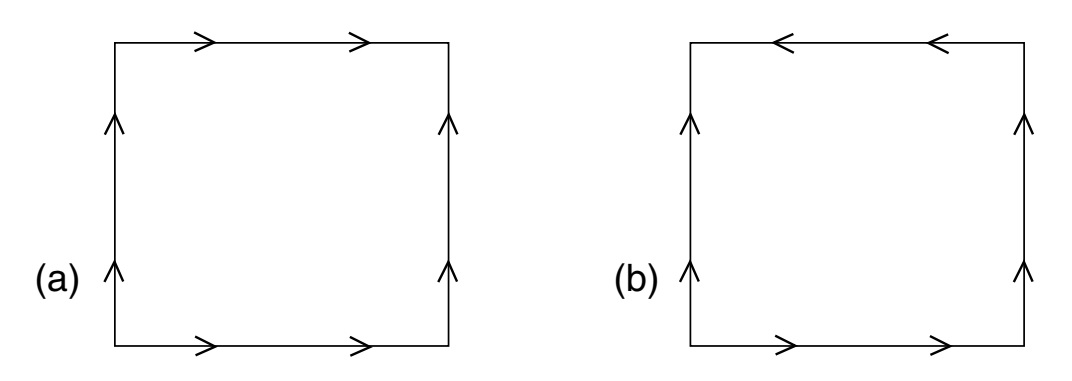
\includegraphics[width=0.8\textwidth,natwidth=750.4,natheight=266.7]{Fig8.6.jpg}
		\caption{粘合对边给出了(a)环面和(b) Klein瓶.}\label{Fig8.6}
	\end{center}
\end{figure}

在画定向弦时, 我们用箭头表示方向. 在非定向理论中, 我们即可省略箭头, 也可取两个方向的线性组合. 
后一个图景与规范化离散对称性的想法更一致, 并且更广泛: 在定向形中, 宇称算符要伴随一个时空变换, 所以我们不能仅仅忘掉箭头.

尽管我们经由$T$-对偶引入了定向形构造, 也可考察那种不是环向紧致化$T$-对偶的更一般定向形, 将世界面宇称与各种时空对称性组合以规范化一个群.

\subsection*{开弦}

在开弦的情况中, 情况是类似的. 简单起见, 我们仅考察一个紧致维的情况. 同之前一样, 在0和 $\pi R^{\prime}$处有定向形不动平面. 
引入 $SO(n)$ Chan-Paton 因子 (辛对称性类似), 一般的威尔逊线可变成对角形式, 当 $n$ 为偶数时, 本征值两两配对: 
\begin{equation}
	W = \operatorname{diag}\left(\me^{\mi \theta_{1}}, \me^{-\mi \theta_{1}}, \me^{\mi \theta_{2}}, \me^{-\mi \theta_{2}}, \cdots, 
								 \me^{\mi \theta_{n/2}}, \me^{-\mi \theta_{n/2}}\right) \:. \label{8.8.4}
\end{equation}
因此, 在对偶图景中, 在线段 $0 \leq X^{\prime 25} \leq \pi R^{\prime}$中有 $\frac{1}{2} n$ 个D膜, 另外 $\frac{1}{2} n$ 个在镜像点. 
弦可以在D-膜和镜像之间张开, 如图\ref{Fig8.7}所示. 一般规范群是 $U(1)^{n/2}$. 同定向理论中相同, 如果$r$个D-膜重合, 则存在$U(r)$规范群. 
如果现在这$r$个D-膜还在其中一个不动平面上, 那么在这些膜中的一个与镜像膜之间张开的弦也是无质量的. 我们就有额外态的正确频谱以填补 $SO(2r)$. 
如果所有膜都在一个定向面上, 就恢复了最大 $SO(n)$.

\begin{figure}
	\begin{center}
		%width=0.8\textwidth,bb=0 0 1030 767
		%1px=0.75pt
		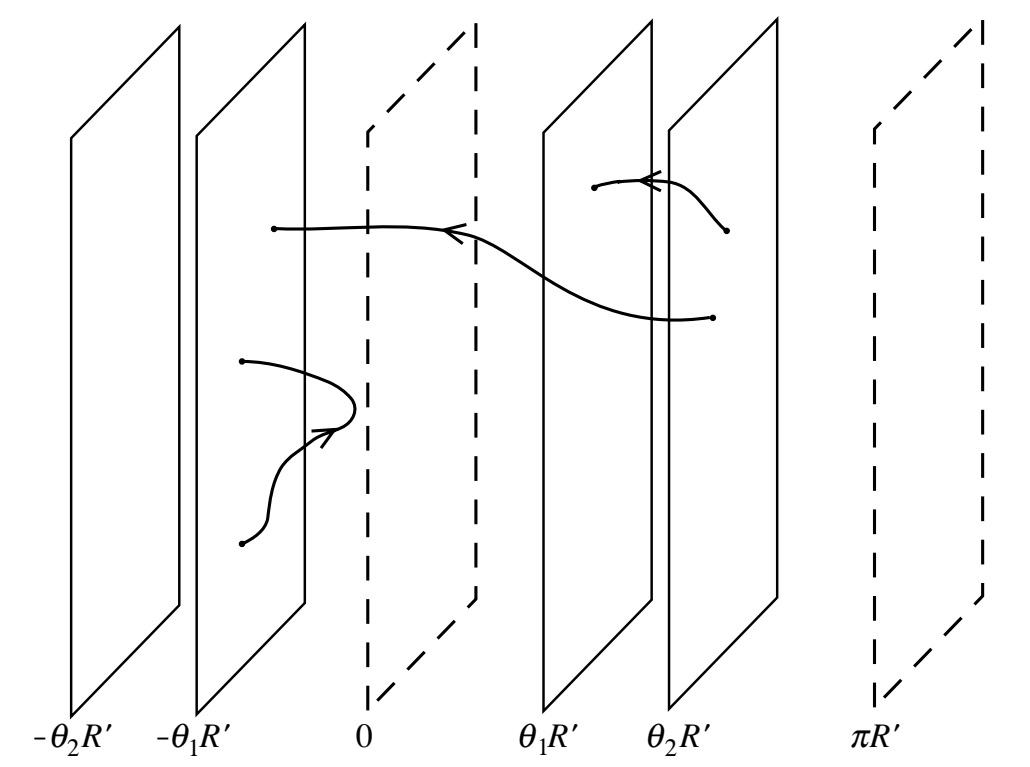
\includegraphics[width=0.6\textwidth,natwidth=721,natheight=555]{Fig8.7.jpg}
		\caption{定向形平面在0处和$\pi R^{\prime}$处, D-膜在$\theta_{1} R^{\prime}$ 和 $\theta_{2} R^{\prime}$处, 
		而D-膜镜像在$-\theta_{1} R^{\prime}$ 和 $-\theta_{2} R^{\prime}$处. 扭挠算符 $\Omega$ 在任何弦上的作用是时空反转的一个组合以及反转定向箭头. 
		%so that the string running from 2 to the image of 1 becomes a string running from 1 to the image of 2.
		}\label{Fig8.7}
	\end{center}
\end{figure}


如果$n$是奇数, $W$ 的最后一个本征值是$\pm 1$, 使得在 $T$-对偶图景中, 固定在两个定向面中的一个. 没有镜像, 这实际是半D-膜. 
另外如果我们考察 $n=2$ 的威尔逊线 $\operatorname{diag}(1,-1)$ (这在 $O(2)$ 而非 $SO(2)$ 中), 那么出现的就不是一个D-膜和它的像, 而是两个半D膜.

同D-膜一样, 定向平面会与伸缩子和度规耦合. 振幅与上节相同, 只不过要用 Klein 瓶和 Möbius 带替换圆环. 
实际上, 我们已经在第\ref{cha:7}章做过相关计算. 在那里我们发现总伸缩子耦合对于$S O\left(2^{13}\right)$抵消了. 
在$T$-对偶图景中, $2^{12}$ 个D-膜的总伸缩子耦合抵消了 (镜像未参与计数). 如果我们对$k=25-p$个维度紧致化, 就会有 $2^{k}$个不动平面, 
它们的坐标是0和$\pi R_{m}^{\prime}$的所有组合. 因此单个不动平面的有效作用量是
\begin{equation}
	2^{12-k} T_{p} \int \dif^{p+1} \xi \: \me^{-\Phi} (-\operatorname{det} G_{ab})^{1/2} \:, \label{8.8.5}
\end{equation}
积分跑遍不动平面.

尽管定向形没有扭挠分区的直接类比, 但是某种意义下, 扭态是开弦. 既然这个类比不是完全的, 我们不倾向于强调这一点: 
规范化 $\Omega$ 自身并不引入世界面边界. 然而, 在定向形理论中加入开弦, 以抵消伸缩子蝌蚪, 却有一定的物理意义. 这个抵消在超弦中将扮演重要角色.

% \setcounter{section}{0}%更改chapter的计数器值
% %\numberwithin{equation}{chapter}%公式计数器从属于节计数器
% \numberwithin{equation}{section}%公式计数器从属于节计数器
% \numberwithin{figure}{section}%图计数器从属于节计数器
% \setcounter{chapter}{8}

%\chapter{\texorpdfstring{高阶振幅}{9 Higher order amplitudes}}
\chapter{高阶振幅} \label{cha:9}
在本章我们将讨论弦论的高阶振幅. 前半段的主要目标是理解弦微扰论的有限性与幺正性. 在细致地讨论树图振幅之后, 我们会考察一般振幅. 
利用因子化的思想将高阶振幅与低阶振幅相关联之后, 我们将讨论一些致力于理解所有阶乃至非微扰弦论的思想.

%\section{\texorpdfstring{一般的树图振幅}{9.1 General tree-level amplitudes}}
\section{一般的树图振幅} \label{sec:9.1}

第\ref{cha:6}章初步考察了某些特定树图振幅的计算. 用一个树图振幅的一般分析展开本章将是有益的, 它将会阐明一些会在高阶振幅出现的模式. 
我们将专注于定向闭弦, 以及三点振幅和四点振幅, 它们会阐明一些重要特征. 主要议题是收敛与``幺正性''. 后一项含义比较宽泛. 
既指S-矩阵的幺正性$S S^{\dagger}=1$, 又指希尔伯特空间的正定性. 当然, 我们从第\ref{cha:4}章已经获知BRST上同调有一个正定内积, 
这使得我们需要证明的是振幅会遵循BRST不变性: 能够出现的只是BRST-不变态, 并且BRST等价态的振幅是相等的. 
对于后者, 我们在\ref{sec:5.4}节给出了一般讨论, 但在这里可以更加清晰地阐释.

在进入一般分析之前, 我们先来回忆一些对计算有用的结果. 假定我们有$d$个无限平坦维, 快子顶点算符归一化成
\begin{equation}
	g_{\mathrm{c}, d} :\mathrel{\me^{\mi k \cdot X}}: \:. \label{9.1.1}
\end{equation}
例如, 在一个维度环向紧致化的情况中, 我们有$g_{\mathrm{c}, 25}=g_{\mathrm{c}}(2 \pi R)^{-1 / 2}$. 
那么, 对于一般OCQ顶点算符的物质部分, 正确的归一化可通过OPE中最奇异的一项固定
\begin{equation}
	\mathscr{V}_{j}(k; z, \bar{z}) \overline{\mathscr{V}_{j^{\prime}}(k; 0,0)} = 
	\frac{g_{\mathrm{c}, d}^{2}}{z^{2} \bar{z}^{2}}+\ldots \:. \label{9.1.2}
\end{equation}
其中加横线代表欧几里得共轭\eqref{6.7.28}. 由于顶点算符权重为(1,1), 奇点是 $|z|^{-4}$. 重复快子极点计算\eqref{6.6.7}就给出归一化
\begin{align}
	& \me^{-2 \lambda} \Bigl\langle \tilde{c}(\bar{z}_{1}) c(z_{1}) \tilde{c}(\bar{z}_{2}) c(z_{2}) \tilde{c}(\bar{z}_{3}) 
	    c(z_{3}) : \mathrel{\me^{\mi k \cdot X}(z, \bar{z})}:\Bigr\rangle \nonumber \\
	&\qquad \qquad \qquad \qquad =\frac{8 \pi \mi}{\alpha^{\prime} g_{\mathrm{c}, d}^{2}} 
	    |z_{12} z_{13} z_{23}|^{2} (2 \pi)^{d} \delta^{d}(k) \:. \label{9.1.3}
\end{align}
所有S-矩阵中的所有归一化常数都写成 $g_{\mathrm{c}, d}=\kappa_{d} / 2 \pi$.

\subsection*{三点振幅}

我们首先将树图振幅表示成几个有用的形式. 对于一般的树图三点振幅, 弦S-矩阵的规范固定表达式\eqref{5.3.9}约化至三个固定顶点算符的路径积分
\begin{equation}
	S_{S_{2}}(1; 2; 3) = \me^{-2 \lambda} \Bigl\langle \hat{\mathscr{V}}_{1}^{\prime}(\infty, \infty) 
	                     \hat{\mathscr{V}}_{2}(1,1) \hat{\mathscr{V}}_{3}(0,0) \Bigr\rangle_{S_{2}} \:, \label{9.1.4}
\end{equation}
其中的数字$n$是弦动量和态$(k_n, j_n)$的缩写. $\hat{}$指明顶点算符处在固定绘景中——即, 对位置的积分不引入$b$鬼场插入. 
正如我们在\ref{sec:5.4}节中讨论的, 这一形式自然地来自于态-算符对应, 并在OCQ情况中取如下的形式
\begin{equation}
	\hat{\mathscr{V}}_{j} = \tilde{c} c \mathscr{V}_{j} \:. \label{9.1.5}
\end{equation}
利用\ref{sec:6.7}节中的结果, 可将球面上的路径积分转化成矩阵元, 这个振幅也可表示成矩阵元或算符乘积系数:
\begin{equation}
	S_{S_{2}}(1; 2; 3) = \me^{-2 \lambda}\lAngle\hat{\mathscr{V}}_{1}|\hat{\mathscr{V}}_{2}(1,1)|\hat{\mathscr{V}}_{3}\rangle
					   = \me^{-2 \lambda} c_{123} \:. \label{9.1.6}
\end{equation}
这将时空中的振幅与世界面上的矩阵元关联起来, 并进一步与编码(encode)CFT定域性质的算符乘积系数相联系. 

第一个议题是BRST-空态的退耦, 这使得BRST-等价态有相同的振幅. 假定三点振幅中的 $|\hat{\mathscr{V}}_{3}\rangle$ 是空态
\begin{equation}
	|\hat{\mathscr{V}}_{3}\rangle=Q_{\mathrm{B}}|\chi\rangle \:. \label{9.1.7}
\end{equation}
那么
\begin{align}
	\me^{2 \lambda} S_{S_{2}}(1; 2; 3) 
	&=  \lAngle \hat{\mathscr{V}}_{1} | [\hat{\mathscr{V}}_{2}(1,1), Q_{\mathrm{B}}] |\chi\rangle        
	   +\lAngle \hat{\mathscr{V}}_{1} | Q_{\mathrm{B}} \hat{\mathscr{V}}_{2}(1,1) |\chi\rangle \nonumber \\
	&=0 \label{9.1.8}
\end{align}
由于态2和1的BRST不变性, 所以它们分别为零. 类似地, 如果 $\hat{\mathscr{V}}_{2}= \{Q_{\mathrm{B}}, \chi\}$ 或 
$|\hat{\mathscr{V}}_{1}\rangle= Q_{\mathrm{B}}|\chi\rangle$, 振幅也为零. 我们已经在这里使用了希尔伯特空间形式理论, 
但值得用路径积分的语言重复相同的讨论. 假定 $\mathscr{V}_{3}$ 在零(null)空间,
\begin{equation}
	\hat{\mathscr{V}}_{3}=Q_{\mathrm{B}} \cdot \mathscr{X}
\end{equation}
将球面上的围道积分扩展, 使之远离 $\mathscr{X}$, 直到它变成绕 $\hat{\mathscr{V}}_{1}$ 的小圈加上绕 $\hat{\mathscr{V}}_{2}$的小圈. 
它们由于BRST不变为零, $Q_{\mathrm{B}} \cdot \hat{\mathscr{V}}_{1}=Q_{\mathrm{B}} \cdot \hat{\mathscr{V}}_{2}=0$.

那么到这一阶, 振幅在物理希尔伯特空间是定义好的, 即BRST上同调. 与时空坐标不变性相对应的空(null)引力子的退耦, 是BRST-空(null)态退耦的特殊情况. 
那么自然会有这样的问题, 时空坐标不变性是否是某个更大对称性的一部分? 我们会在\ref{sec:9.6}节回到这个问题. 

我们现在考察S-矩阵的幺正性
\begin{equation}
	\sum_{n} S_{mn} S_{pn}^{*} \questeq \delta_{mp} \:, \label{9.1.10}
\end{equation}
这等价于几率守恒. 将S-矩阵拆成常数项与散射项
\begin{equation}
	S_{mn} = \delta_{mn} + \mi T_{mn} \:. \label{9.1.11}
\end{equation}
那么对于散射矩阵$T$, 幺正性暗示了
\begin{equation}
	T_{mp} - T_{pm}^{*} = \mi \sum_{n} T_{mn} T_{pn}^{*} \:. \label{9.1.12}
\end{equation}

根据定义, $T$-矩阵至少包括三个粒子, 所以对于球面上的三粒子振幅, \eqref{9.1.12}的右边为零. 那么幺正性给出
\begin{equation}
	T_{S_{2}}(1; 2; 3) = T_{S_{2}}(-1; -2; -3)^{*} \:, \label{9.1.13}
\end{equation}
其中负号代表将入顶点算符换成出顶点算符. 如果入顶点算符与出顶点算符之间的关系是
\begin{equation}
	\hat{\mathscr{V}}_{-i}=-\overline{\hat{\mathscr{V}}}_{i} \:. \label{9.1.14}
\end{equation}
那么 \eqref{9.1.13} 就是满足的. 这是一个自然的定义: 共轭将 $\me^{\mi k \cdot X}$ 变成 $\me^{-\mi k \cdot X}$, 出射变入射, 对于其他量子数类似. 
引入负号是为了抵消$\tilde{c} c$ 顺序的调换, 这使得 $\hat{\mathscr{V}}_{-i}$ 仅是对顶点算符所有显含$\mi$的因子取共轭. 那么路径积分的共轭给出
\begin{equation}
	\Bigl\langle \hat{\mathscr{V}}_{1}^{\prime}(\infty,\infty) \hat{\mathscr{V}}_{2}(1,1) \hat{\mathscr{V}}_{3}(0,0)\Bigr\rangle_{S_{2}}=-\Bigl\langle\hat{\mathscr{V}}_{-1}^{\prime}(\infty,\infty) \hat{\mathscr{V}}_{-2}(1,1) 
	\hat{\mathscr{V}}_{-3}(0,0)\Bigr\rangle_{S_{2}}^{*} \:, \label{9.1.15}
\end{equation}
这暗示了幺正关系\eqref{9.1.13}. 想当然的看, 这个路径积分显然是实的, \eqref{9.1.15}中不应有负号. 
但是, 我们记起这个路径积分必须通过特定的解析延拓定义, 而显式结果\eqref{6.2.6}因此获得总因子$\mi$.

\subsection*{四点振幅和世界面对偶}

连通四点振幅是
\begin{equation}
	S_{S_{2}}(1; 2; 3; 4) = \me^{-2 \lambda} \int_{\mathds{C}} \dif^{2} z 
	\Bigl\langle \hat{\mathscr{V}}_{1}^{\prime}(\infty, \infty) \hat{\mathscr{V}}_{2}(1,1) \hat{\mathscr{V}}_{3}(0,0) 
	                  \mathscr{V}_{4}(z, \bar{z})\Bigr\rangle_{S_{2}} \:. \label{9.1.16}
\end{equation}
将这一期望值写成一个矩阵元给出
\begin{equation}
	\lAngle\hat{\mathscr{V}}_{1}|\mathrm{T}[\hat{\mathscr{V}}_{2}(1,1) \mathscr{V}_{4}(z, \bar{z})]| 
	\hat{\mathscr{V}}_{3}\rangle \:. \label{9.1.17}
\end{equation}
对于OCQ顶点算符, 鬼场期望值是常数. 但为了与普遍情况相联系, 将这个鬼场稍微移动一点更有用. 利用围道讨论, 对 $\dif^{2} z$积分的鬼场插入可以写成
\begin{equation}
	\mathscr{V}_{4}(z, \bar{z})=(z \bar{z})^{-1}\bigl \{b_{0}, [\tilde{b}_{0}, \hat{\mathscr{V}}_{4}(z, \bar{z})]\bigr\} \:. \label{9.1.18}
\end{equation}
利用上式以及  $b_{0}$与 $\tilde{b}_{0}$湮灭物理态的条件\eqref{4.3.29}, 矩阵元变成
\begin{align}
&\theta(1-|z|) \lAngle \hat{\mathscr{V}}_{1} |\hat{\mathscr{V}}_{2}(1,1) b_{0} \tilde{b}_{0} z^{L_{0}-1} \bar{z}^{\tilde{L}_{0}-1} 
                       \hat{\mathscr{V}}_{4}(1,1)| \hat{\mathscr{V}}_{3}\rangle  \nonumber \\
&\qquad + \theta(|z|-1) \lAngle\hat{\mathscr{V}}_{1}|\hat{\mathscr{V}}_{4}(1,1) b_{0} \tilde{b}_{0} z^{-L_{0}-1} 
                        \bar{z}^{-\tilde{L}_{0}-1} \hat{\mathscr{V}}_{2}(1,1)|\hat{\mathscr{V}}_{3}\rangle \:. \label{9.1.19}
\end{align}
我们在矩阵元中插入中间态的完备基
\begin{align}
	&\quad \theta(1-|z|) \sum_{i, i^{\prime}} z^{\alpha^{\prime}(k_{i}^{2}+m_{i}^{2})/4 - 1} 
	                                          \bar{z}^{\alpha^{\prime}(k_{i}^{2}+\tilde{m}_{i}^{2})/4 - 1} \nonumber  \\[-12pt] 
	& \qquad \qquad \qquad \qquad \times \lAngle \hat{\mathscr{V}}_{1}|\hat{\mathscr{V}}_{2}(1,1) b_{0} \tilde{b}_{0}|i\rangle 
	  \mathscr{G}^{i i^{\prime}} \lAngle i^{\prime} |\hat{\mathscr{V}}_{4}(1,1)| \hat{\mathscr{V}}_{3}\rangle  \nonumber \\[5pt]
	&+ \theta(|z|-1) \sum_{i, i^{\prime}} z^{-\alpha^{\prime}(k_{i}^{2}+m_{i}^{2})/4 - 1} 
	                   \bar{z}^{-\alpha^{\prime}(k_{i}^{2}+\tilde{m}_{i}^{2})/4 - 1} \nonumber \\[-12pt] 
	& \qquad \qquad \qquad \qquad \times \lAngle \hat{\mathscr{V}}_{1} |\hat{\mathscr{V}}_{4}(1,1) b_{0} \tilde{b}_{0}|i\rangle 
	   \mathscr{G}^{i i^{\prime}} \lAngle i^{\prime}|\hat{\mathscr{V}}_{2}(1,1)|\hat{\mathscr{V}}_{3}\rangle \:. \label{9.1.20}
\end{align}

在后一种形式中, 积分在 $z \rightarrow 0$处的行为是显然的, 并且它与我们在第\ref{cha:6}章研究的快子振幅相同. 
如果 $k_{i}^{2}+m_{i}^{2}$ 和 $k_{i}^{2}+\tilde{m}_{i}^{2}$对所有 $i$为正, 即
\begin{equation}
	k_{i}^{2}=\left(k_{1}+k_{2}\right)^{2}>\frac{4}{\alpha^{\prime}} \:, \label{9.1.21}
\end{equation}
那么积分收敛. 在别处, 它像\eqref{6.6.7}中那样定义
\begin{equation}
	\int_{|z|<1} \dif^{2} z \: z^{\alpha^{\prime}(k^{2}+m^{2})/4 - 1} \bar{z}^{\alpha^{\prime}(k^{2}+\tilde{m}^{2})/4 - 1}
	 =\frac{8 \pi}{\alpha^{\prime}} \frac{\delta_{m^{2}, \tilde{m}^{2}}}{k^{2} + m^{2} - \mi \epsilon} \:. \label{9.1.22}
\end{equation}
可以认为这是从很大的正 $m^{2}$值解析延拓. 类似的, $z \rightarrow \infty$ 的积分对于$(k_{1}+k_{4})^{2}>4 / \alpha^{\prime}$收敛, 
而在其余地方通过解析延拓定义. 若研究的是$z \rightarrow 1$的极限, \eqref{9.1.20}是无用的. 取而代之, 利用振幅的对称性交换顶点算符2和3. 
那么 $z \rightarrow 1$ 的积分通过从收敛区域 $(k_{1}+k_{3})^{2}>4 / \alpha^{\prime} $解析延拓定义.

像\eqref{9.1.22}那样对\eqref{9.1.20}积分后, 振幅表示成 $s$和 $u$极点的级数. 我们从第\ref{cha:6}章知道, 这个振幅也有$t$的极点, 但这并不显然: 
它们来自无限求和的发散. 类似的开弦振幅 $I(s, t)$ 有$s$和 $t$的极点, 但它可以写成 $s$或 $t$的无限求和. 
这一性质称为\emph{对偶}, 或者\emph{世界面对偶}. 我们可以认为它来自于沿不同的曲线切开世界面, 这代表以不同的方式对中间态求和. 
另外一个例子是对开弦态求和给出圆柱上的闭弦极点.

\subsection*{四点振幅幺正性}

我们现在来验证四点振幅对于等价态是相等的. 令 $|\hat{\mathscr{V}}_{3}\rangle=Q_{\mathrm{B}}|\chi\rangle$ 是空(null)态. 
利用\eqref{9.1.19}, 我们将 $Q_{\mathrm{B}}$ 交换至左边, 直至它湮灭 $\lAngle\hat{\mathscr{V}}_{1}|$. 
BRST算符与 $L_{0}, \tilde{L}_{0}$及 顶点算符对易, 但与 $b_{0}$和 $\tilde{b}_{0}$不对易. 非零对易子包括
\begin{equation}
	\Bigl[b_{0} \tilde{b}_{0} z^{\pm L_{0}-1} \bar{z}^{\pm \tilde{L}_{0}-1}, Q_{\mathrm{B}}\Bigr] = 
	\pm b_{0} \partial_{\bar{z}}\Bigl(z^{\pm L_{0}-1} \bar{z}^{\pm \tilde{L}_{0}}\Bigr) \mp 
	\tilde{b}_{0} \partial_{z}\Bigl(z^{\pm L_{0}} \bar{z}^{\pm \tilde{L}_{0}-1}\Bigr) \:. \label{9.1.23}
\end{equation}
它们是全导数, 例证了一般性原理 \eqref{5.4.6}: 空(null)态的耦合正比于模空间上的导数. 对于\ref{sec:6.6}节中的无质量顶点算符我们看到了这样的例子. 
在那个例子中, 积分由于抵消传播子的讨论为零. $z \rightarrow 0$处的积分通过从很大的正 $(k_{1} + k_{2})^{2}$ 处解析延拓获得. 
表面项在那里恒为零, 所以根据解析性处处为零. 相同的讨论适用于模空间的其他极限.

对于球面上的四点振幅, 幺正性条件是
\begin{align}
& T_{S_{2}}(1; 2; 3; 4) - T_{S_{2}}(-1; -2; -3; -4)^{*} \nonumber \\
& \quad = \mi \sum_{j_{5}} \int \frac{\dif^{d-1} \mathbf{k}_{5}}{2 E_{5}(2 \pi)^{d-1}} T_{S_{2}}(1; 2; 5) T_{S_{2}}(-5; 3; 4)
           + \text{2个置换} \nonumber \\
& \quad = -\mi \me^{-4 \lambda} \sum_{j_{5}} \int \frac{\dif^{d-1} \mathbf{k}_{5}}{2 E_{5}(2 \pi)^{d-1}}
          \lAngle\hat{\mathscr{V}}_{1} |\hat{\mathscr{V}}_{2}(1,1)| \hat{\mathscr{V}}_{5}\rangle 
		  \lAngle\hat{\mathscr{V}}_{-5}|\hat{\mathscr{V}}_{3}(1,1)| \hat{\mathscr{V}}_{4}\rangle  \nonumber \\
& \qquad + \text{2个置换} \: . \label{9.1.24}
\end{align}
中间粒子在壳, 对 $j_{5}$ 求和取遍将1234分成两对的所有方式: 12-34, 13-24, 和 14-23.

\eqref{9.1.24} 是我们希望证明的. 在矩阵元\eqref{9.1.20}中使用实条件\eqref{9.1.13}, 在$z$积分收敛区域内, \eqref{9.1.24}的左边为零. 
非零部分来自解析延拓时引入的$\mi \epsilon$,
\begin{equation}
	\frac{1}{k^{2} + m^{2} - \mi \epsilon} - \frac{1}{k^{2}+m^{2}+ \mi \epsilon}=2 \pi \mi \delta(k^{2}+m^{2}) \:. \label{9.1.25}
\end{equation}
因此
\begin{align}
		& T_{S_{2}}(1; 2; 3; 4) - T_{S_{2}}(-1; -2; -3; -4)^{*} \nonumber \\
		&\quad =\frac{16 \pi^{2} \mi}{\alpha^{\prime} \me^{2 \lambda}} 
		\sum_{i, i^{\prime}} \delta_{m_{i}^{2}, \tilde{m}_{i}^{2}} \delta(k_{i}^{2}+m_{i}^{2})
		\lAngle\hat{\mathscr{V}}_{1}|\hat{\mathscr{V}}_{2}(1,1) b_{0} \tilde{b}_{0}| i\rAngle \mathscr{G}^{i i^{\prime}} 
		\lAngle i^{\prime} |\hat{\mathscr{V}}_{3}(1,1)| \hat{\mathscr{V}}_{4}\rangle \nonumber \\
		&\qquad +\text{2个置换.} \label{9.1.26}
\end{align}
这很像希望得到的幺正关系\ref{9.1.24}, 还需要一点处理来完成这个结果. 求和\eqref{9.1.26}中的指标$i$取遍弦态的完备基, 标记了内部态和动量
\begin{equation}
	i \leftrightarrow(j, k) \:. \label{9.1.27}
\end{equation}
\eqref{9.1.26}中引入的$\delta$-函数与 $b_{0} \tilde{b}_{0}$因子投射到被 $L_{0}, \tilde{L}_{0}, b_{0}$和 $\tilde{b}_{0}$湮灭的空间$\hat{\mathscr{H}}$, 这在BRST上同调的讨论中引入过. 因此
\begin{align}
	&\sum_{i, i^{\prime}} \delta_{m_{i}^{2}, \tilde{m}_{i}}^{2} \delta(k_{i}^{2}+m_{i}^{2}) b_{0} \tilde{b}_{0}
	    				  |i\rangle \mathscr{G}^{i i^{\prime}}\lAngle i^{\prime}| \nonumber  \\
	&\qquad =\delta_{L_{0}, \tilde{L}_{0}} \delta(4 L_{0} / \alpha^{\prime}) b_{0} \tilde{b}_{0}  \nonumber \\
	&\qquad =-\frac{\mi \alpha^{\prime}}{16 \pi^{2} \me^{2 \lambda}} \int \frac{\dif^{d-1} \mathbf{k}}{2 E(2 \pi)^{d-1}} 
	 \sum_{j \in \hat{\mathscr{H}} \atop k^{0}=\pm \omega_{k}}
	 |\hat{\mathscr{V}}_{j}(k)\rangle \lAngle\overline{\hat{\mathscr{V}}_{j}(k)}| \:. \label{9.1.28}
\end{align}
基$|\mathscr{V}_{j}(k)\rangle$的归一化可从OPE\eqref{9.1.2}和期望值\eqref{9.1.3}得出, 这给出
\begin{equation}
	\lAngle\overline{\hat{\mathscr{V}}_{j}(k)}|\tilde{c}_{0} c_{0}| \hat{\mathscr{V}}_{j^{\prime}}(k^{\prime})\rangle = 
	\frac{8 \pi \mi \me^{2 \lambda}}{\alpha^{\prime}} \delta_{j j^{\prime}}(2 \pi)^{d} \delta^{d}(k-k^{\prime}) \:. \label{9.1.29}
\end{equation}

利用\eqref{9.1.28}可以看到\eqref{9.1.26}的形式、归一化与幺正性条件\eqref{9.1.24}完全一致, 只留下一个缺口. 
幺正关系中的求和只取遍物理态空间, 即BRST上同调, 而\eqref{9.1.28}中的最终求和取遍 $\hat{\mathscr{H}} $ 的一个完备基. 
我们现在证明这些和是相等的. 考察$\hat{\mathscr{H}}$如下的基. 
首先, 取``非物理态'' $|a\rangle_{\mathrm{U}} $ 的完备基, 即, 它们的线性组合不会被$Q_{\mathrm{B}}$湮灭.
第二, 取BRST不变态 $|b\rangle_{\mathrm{P}}$ 的完备基, 它们是线性独立的, 即它们的线性组合不会是空(null)态.
最后, 取BRST-空(null)态 $|a\rangle_{\mathrm{N}}=Q_{\mathrm{B}}|a\rangle_{\mathrm{U}}$, 整个基就完成了. 
定义算符 $\mathscr{P}$ 和 $\mathscr{U}$ :
\begin{subequations} \label{9.1.30}
\begin{align}
	&\mathscr{P}|b\rangle_{\mathrm{P}} = |b\rangle_{\mathrm{P}}, \quad \mathscr{P}|a\rangle_{\mathrm{U}}=0, \quad 
	 \mathscr{P}|a\rangle_{\mathrm{N}} = 0 \:; \label{9.1.30a} \\
	&\mathscr{U}|b\rangle_{\mathrm{P}} = 0, \quad \mathscr{U}|a\rangle_{\mathrm{U}}=0, \quad 
	 \mathscr{U}|a\rangle_{\mathrm{N}} = |a\rangle_{\mathrm{U}} \:. \label{9.1.30b}
\end{align}
\end{subequations}
那么
\begin{equation}
	1=\mathscr{P}+Q_{\mathrm{B}} \mathscr{U}+\mathscr{U} Q_{\mathrm{B}} \:. \label{9.1.31}
\end{equation}
将这一分解插入因子化关系. 第一项将每个态投射到每个上同调态中, 物理频谱出现在幺正和中. 
第二项和第三项均包含 $Q_{\mathrm{B}}$, 由于之前空(null)态退耦的讨论, 它们为零. 因此幺正性得以建立.

值得注意的是, 这个讨论与规范理论中的振幅既洛伦兹不变又幺正的讨论十分相似. 协变光子传播子
\begin{equation}
	-\mi \frac{\eta^{\mu \nu}}{k^{2}} \:, \label{9.1.32}
\end{equation}
它的分子的本征值为负, 对应负范的中间态. 选择任意使得$n \cdot k=1$的空(null)矢量$n^{\mu}$, 并作分解
\begin{equation}
	\eta^{\mu \nu}=(\eta^{\mu \nu}-k^{\mu} n^{\nu}-n^{\mu} k^{\nu}) + k^{\mu} n^{\nu}+n^{\mu} k^{\nu} \:. \label{9.1.33}
\end{equation}
当 $k^{2}=0$, 第一项有 $d-2$ 个正本征值, 没有负本征值. 如果光子在两端与守恒流耦合, 后两项为零, 所以幺正关系是满足的. 
分解\eqref{9.1.31}是 \eqref{9.1.33}的推广: $k^{\mu} \rightarrow|a\rangle_{\mathrm{N}}$ 且 $n^{\mu} \rightarrow|a\rangle_{\mathrm{U}}$.

我们现在进行总结, 我们来回顾一下各种一般性原理在例子中是如何阐明的. BRST空(null)态退耦, 但这在模空间积分后. 
来自后者的势表面项由于抵消传播子讨论为零. 给出\eqref{9.1.19}的鬼场处理在第\ref{cha:5}章的黎曼面图景下有一个自然的解释. 
考察顶点算符在$0,1, z, \infty $处的球面. 更具体的, 取 $|z|>1$ , 就像\eqref{9.1.19}的第二项. 我们可以认为这个球面由两个圆盘构成, 
坐标为 $z_{1}$和$z_{2}$. 将顶点算符放在 $z_{1}=0,1$ 和 $z_{2}=0,1$, 并用等价关系$z_{1}=z / z_{2}$连接两个圆盘. 对于模 $z$, 我们有
\begin{equation}
	\frac{\partial z_{1}}{\partial z}\biggr|_{z_{2}}=\frac{z_{1}}{z} \:. \label{9.1.34}
\end{equation}
对于 $\dif z$ 的鬼场插入 \eqref{5.4.15} 就是 $b_{0} / z$, 对$\dif \bar{z}$类似. 这正是 \eqref{9.1.19}中例证的.


\section{高亏格黎曼面} \label{sec:9.2}%{9.2 Higher genus 黎曼 surfaces}

对于高亏格黎曼面, 有很多不同的表示. 对于我们的目的而言, 其中最有用的一个是将低亏格黎曼面缝在一起制造高亏格黎曼面. 
这将在下节讨论, 但为了完整起见, 我们先来描述几个通用的构造.

\subsection*{Schottky 群}

假想从球面上移去两个圆盘, 并将形成的洞粘起来. 这产生一个把手, 所以以这种方式获得的曲面是环面. 重复$g$ 次, 就生成了亏格为 $g$ 的曲面.

我们可以将其做的更精细一些. 视球面为复 $z$平面加无穷远点, 考察映射
\begin{equation}
	\gamma: \quad \frac{z^{\prime}-U}{z^{\prime}-V}=K \frac{z-U}{z-V} \:, \label{9.2.1}
\end{equation}
它依赖3个复参量 $U$, $V$, $K$. 这是Möbius变换, 特别地, 这是全纯的且1到1的. 点 $U$, $V$在 $\gamma $ 下不动. 
取 $|K|>1$, 这个平面从$U$处延展向 $V$收缩.  $\gamma$ 的基本域是圆环
\begin{equation}
	|K|^{-1/2} < \left|\frac{z-U}{z-V}\right| < |K|^{1/2} \:. \label{9.2.2}
\end{equation}
等同 $\gamma$下的点, 将圆环\eqref{9.2.2}的内外边界粘在一起, 这产生了环面. 由 $g$个元素\eqref{9.2.1}生成的群产生了亏格为 $g$ 的的曲面, 
对于参量的约束要使缝合圆不重合.

每个定向闭黎曼面都可以用这种方式获得. 不过参量的区域并不简单, 其中的部分原因是某些模变换的方式非常复杂. 
有边界的黎曼面和非定向的黎曼面可以通过用闭黎曼面除以一个或两个反射获得, 我们在低亏格的例子中例证过这一点.

我们来看一下 Schottky 构造确实产生了期待的模的数目. 每个变换\eqref{9.2.1}有3个复参量, 那么总的复参量个数就是 $3 g$. 
我们可以认为每个柄有6个实参量, 其中每个洞的位置需要2个实参量. 两个洞的半径之积需要1个, 还有1个用来描述缝合两个洞时的相对角. 
由于球面上的一个总 Möbius 变换给出等价的球面, 存在冗余. 减掉这个群的6个实参量, 还剩 $6 g-6$, 与 $g \geq 2$ 的模数目相同. 
当 $g=1$时, 有两个Möbius变换使得映射不变, 所以剩下两个实参量.

Schottky参量化表明模空间有自然的复坐标. 尽管我们没有强调这一点, 但路径积分相对这些坐标有特定的全纯性. 
在将一般曲面构造为球面的陪集后, 先用镜像法, 再对所有源的像求和就可得到格林函数. 泛函行列式以及其他感兴趣的量可以用类似的方法描述出来.

\subsection*{Fuchsian群}

对于这一构造, 首先考察世界面度规. 有一个定理: 通过Weyl变换, 总可以使世界面曲率$R$为常数. 亏格为0给出球面, 亏格为1给出环面. 
在高亏格, 则给出负常曲率的曲面. 对于所有这些曲面, 它们的单连通覆盖空间类似地有常曲率. 精确存在3个这样的单连通空间——圆球、平面(环面的覆盖空间)以及度规如下的上半平面
\begin{equation}
	\dif s^{2}=\frac{\dif z \dif \bar{z}}{(\operatorname{Im} z)^{2}} \:. \label{9.2.3}
\end{equation}
最后一个是所有亏格$g \geq 2$ 曲面的覆盖空间.

相应地, 所有亏格$g \geq 2$的曲面可以通过用某些离散群的作用除上半平面获得. 这个群的元素必须是度规 \eqref{9.2.3} 的等距变换; 
这些等距变换就是实系数的Möbius变换, $PSL(2, \mathds{R})$. 图\ref{Fig9.1}给出了亏格为3的曲面, 上面有一些闭合曲线. 对于每个柄有 $A$ 闭链和 $B$闭链. 
它们是非平庸曲线, 即无法收缩到一点. 如果我们横穿其中一条曲线, 在覆盖空间上我们不回到原点而是等价于它的曲线. 
因此对于每个闭链, 我们赋予 $PSL(2, \mathds{R})$的一个元素, 也记为 $A_{i}$或 $B_{i}$.

\begin{figure}
	\begin{center}
		%width=0.8\textwidth,bb=0 0 1218 388
		%1px=0.75pt
		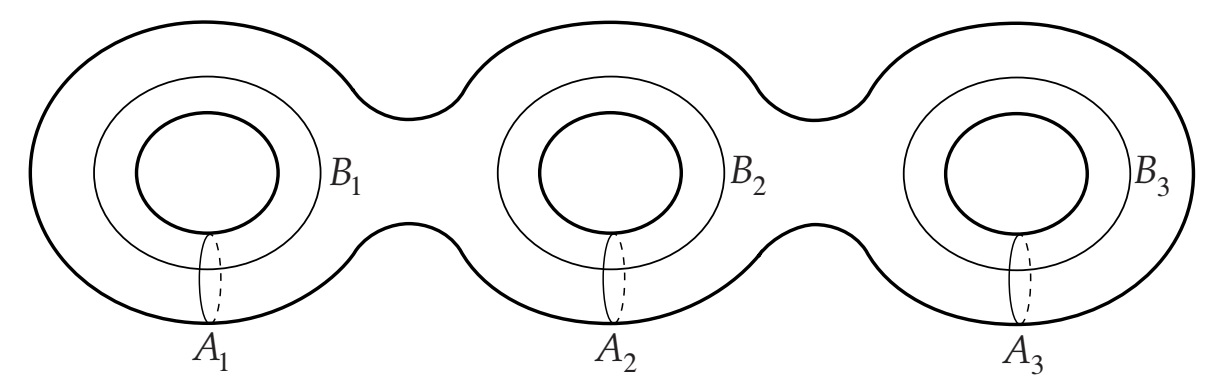
\includegraphics[width=0.8\textwidth,natwidth=852.6,natheight=271.6]{Fig9.1.jpg}\\
		\caption{亏格为3的曲面, 上面标出了$A$-闭链和$B$-闭链.}\label{Fig9.1}
	\end{center}
\end{figure}


$A$-闭链和$B$-闭链是完备的, 在每个闭合路径都同伦(homotopic)等价于一连串的 $A$ 闭链或 $B$闭链. 事实上, 它们是过完备的: 路径
\begin{equation}
	(A_{1} B_{1}^{-1} A_{1}^{-1} B_{1})(A_{2} B_{2}^{-1} A_{2}^{-1} B_{2}) \ldots(A_{g} B_{g}^{-1} A_{g}^{-1} B_{g}) \label{9.2.4}
\end{equation}
可收缩到一点, 并且相应乘积必须是单位元. 对模计数, 在每个 $PSL(2, \mathds{R})$ 元素中有6个实参量, 给出$6g$, 从约束\eqref{9.2.4}中减去3个, 
由于总的$PSL(2, \mathds{R})$ 给出等价曲面, 再减去3个, 总共$6g-6$ .

尽管Schottky参量化与Fuchsian参量化类似, 但它们有相当不同的性质. 特别地, 后者的复结构不那么显然, 相应地, 到超弦的扩张也就不那么简单.

\subsection*{周期矩阵}
环面的模参量 $\tau$ 在亏格为$g$时可以自然地推广至 $g \times g$ 矩阵. 为看到这一点, 我们首先需要阿贝尔微分或全纯1-形式. 
它们是世界面场 $\omega_{a}$, 在复坐标中拥有如下性质
\begin{equation}
	\partial_{\bar{z}} \omega_{z} = 0 \:, \quad \omega_{\bar{z}} = 0 \:. \label{9.2.5}
\end{equation}
精确有 $g$个这样的场, 并且 $g$ 进一步满足共轭关系. 这源于黎曼-罗赫定理\eqref{5.3.22}. 阿贝尔微分 \eqref{9.2.5} 及其共轭正是算符$P_{0}^{T}$的核, 
对此, 黎曼-罗赫定理是
\begin{equation}
	\operatorname{dim} \operatorname{ker} P_{0}^{T}-\operatorname{dim} \operatorname{ker} P_{0}=-\chi=2 g-2 \:. \label{9.2.6}
\end{equation}
算符 $P_{0}$ 作用在 $h=0$的标量场 $c$和$\tilde{c}$上, 因而退化至普通的梯度. 这总有2个零模 ($c=$常数或者$\tilde{c}=$常数), 
因而$\operatorname{dim}\operatorname{ker}P_{0}^{T}=2 g$.

1-形式的线积分是坐标不变量. 那么阿贝尔微分的自然基就是 $\omega_{z i}, i=1, \ldots, g$, 定义成
\begin{equation}
	\oint_{A_{i}} \dif z \: \omega_{z j}=\delta_{i j} \:. \label{9.2.7}
\end{equation}
那么周期矩阵
\begin{equation}
	\tau_{i j}=\oint_{B_{i}} \dif z\: \omega_{z j} \label{9.2.8}
\end{equation}
表征了曲面的复结构. 当亏格为1时, $\omega_{z}$ 是常数, 这是通常的$\tau$.

可以证明 $\tau_{ij}$ 是对称的, 所以它有 $\frac{1}{2} g(g+1)$ 个复参量. 当 $g=1,2,3$ 它等于复模的个数. 
当 $g \geq 4$ 时, 它会大一些, 所以不是所有周期矩阵都对应黎曼面. $\theta$-函数 \eqref{7.2.36} 有一个自然的亏格-g推广, 
那时 $\tau$ 变成周期矩阵,  $\nu, n, a, b$ 变成 $g$分量矢量.

\subsection*{超椭圆曲面}

还有一种描述, 有时是非常有用的. 考察空间 $S_{2} \times S_{2}$, 坐标分别为 $z$ ,  $y$. 考察如下方程给定的子流形
\begin{equation}
	y^{2}=\prod_{i=1}^{2 k}(z-Z_{i}) \:, \label{9.2.9}
\end{equation}
$Z_{i} $是复参量. 投射到 $z$坐标上, 存在$k$ 个割线相连的两个曲面. 这给出有 $g=k-1$ 个柄的曲面. 当投射到 $z$时, 支点是奇异的, 
但整个曲面\eqref{9.2.9}不奇异: $y$是定域好坐标.

这个曲面依赖$2 k$ 个复$Z_{i}$, 但其中一些在 Möbius变换下冗余, 留下 $2 k-3=2 g-1$个复参量. 当 $g=1,2$, 这与模的个数相同; 
但 $g \geq 3$ 时, 模的个数更多一些, 只有特殊的曲面有\eqref{9.2.9}的形式, 它们被称为超椭圆曲面.

\section{世界面的缝合与切割}  \label{sec:9.3}%{9.3 Sewing and cutting world-sheets}

在分析弦振幅时, 一个有用的概念是高亏格振幅与低亏格振幅之间的关系. 其中的关键要素是排水管(plumbing fixture). 
这用来从低亏格曲面构建高亏格曲面. 考察两个世界面$M_{1}$,  $M_{2}$, 坐标分别为$z_{1}$, $z_{2}$. 
我们可以连接它们构成新的世界面$M$. 方法如下: 令$q$是复参量. 从 $M_{1}$ 上减掉圆盘 $|z_{1}|<(1-\epsilon)|q|^{1/2}$ , 
从 $M_{2}$ 减掉 $|z_{2}|<(1-\epsilon)|q|^{1/2}$, $\epsilon$为一小量. 为了构成一个面, 等同点, 使得
\begin{equation}
	z_{1} z_{2}=q \:. \label{9.3.1}
\end{equation}
如图\ref{Fig9.2}所示. 圆盘区域
\begin{equation}
	(1-\epsilon)^{-1}|q|^{1/2} > |z_{1}| > (1-\epsilon)|q|^{1/2} \label{9.3.2}
\end{equation}
像图中所示的那样缝合在一起. 这一构造的一个表示是
\begin{equation}
	M=M_{1} \infty M_{2}(z_{1}, z_{2}, q) \:. \label{9.3.3}
\end{equation}
这个符号强调了相应曲面依赖于定域坐标的选择. 若选择不同的定域坐标$z_{1}^{\prime}$ 和 $z_{2}^{\prime}$, 将会剪掉不同的圆, 并且连接曲面一般不同. 
这两个坐标卡也可能处在单个曲面$M_{0}$的不同部分. 那么排水管构造给曲面加了一个柄. 这记为
\begin{equation}
	M=M_{0} 8(z_{1}, z_{2}, q)  \:. \label{9.3.4}
\end{equation}
符号`$\infty$'和`8'用来区分两种缝合过程. 参量$q$实际上是不需要的——取$z_{1}^{\prime}=z_{1} q^{-1/2}$, $z_{2}^{\prime}=z_{2} q^{-1/2}$, 
和$q^{\prime}=1$给出等价曲面. 引入$q$是为了方便讨论坐标卡固定时, 随着$q$变化的行为.

\begin{figure}
	\begin{center}
		%width=0.8\textwidth,bb=0 0 877 729
		%1px=0.75pt
		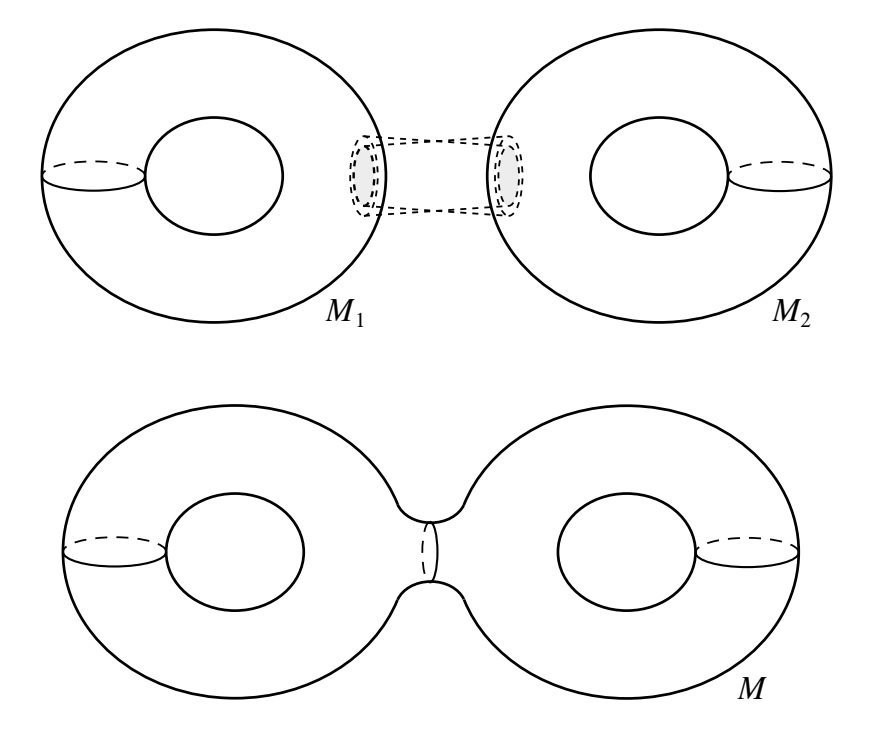
\includegraphics[width=0.6\textwidth,natwidth=613.9,natheight=530]{Fig9.2.jpg}\\
		\caption{从两个世界面上各挖掉一个圆盘然后讲圆盘边粘起来.}\label{Fig9.2}
	\end{center}
\end{figure}

我们也可以逆转这一构造. 给定任意的黎曼面$M$, 以及上面的不相交曲线$C$ , 总可以在$C$的邻域内找到全纯坐标得$z_{1}=z_{2}^{-1}$, 
使得 $C$由 $|z_{1}| = |z_{2}| = |q|^{1/2}$给出. 剪切 $C$ (撤销等价关系 $z_{1} z_{2}=q)$ 并粘回圆盘$|z_{1}|<|q|^{1/2}$和$|z_{2}|<|q|^{1/2}$, 
这产生了 $M_{1}$和 $M_{2}$(或 $M_{0}$), 使得 $M$可以通过缝合操作重新产生——取决于剪切$C$是否使得曲面非连通, 我们分别使用缝合\eqref{9.3.3}或\eqref{9.3.4}.


\begin{figure}[h]
	\begin{center}
		%width=0.8\textwidth,bb=0 0 994 578
		%1px=0.75pt
		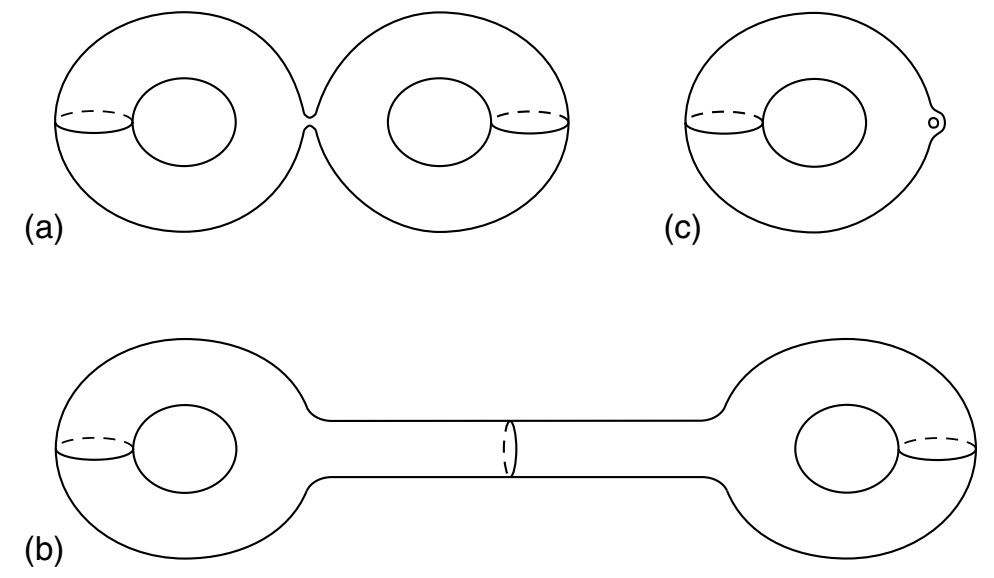
\includegraphics[width=0.6\textwidth,natwidth=695.8,natheight=420]{Fig9.3.jpg}\\
		\caption{带有退化圆的亏格2曲面的三个表示.}\label{Fig9.3}
	\end{center}
\end{figure}

对于图\ref{Fig9.2}中亏格为2的例子, 考察$q \ll 1$的情况. 图\ref{Fig9.3}a给出了这一情况下的 $M$. 
在重叠区域, 我们在$\dif z_{1} \dif \bar{z}_{1}$ 和 $\dif z_{2} \dif \bar{z}_{2}$之间光滑地插入了度规. 
曲面被捏成了半径量级为 $|q|^{1/2} $ 的圆. 通过一个Weyl变换, 总可以找到一个度规, 使得半径保持量级为1, 如图\ref{Fig9.3}b所示. 
既然 Weyl 变换的作用是等距的, 其效应是柄的长度变得很大, 量级为$-\ln |q|$. 柄区域$|z_{1}|<1$, $|z_{2}|<1$ 等效于圆柱
\begin{equation}
	\ln |q|<\operatorname{Im} w<0 \:, \quad w \cong w+2 \pi \:. \label{9.3.5}
\end{equation}
其中 $z_{1}=\exp (-\mi w)$ and $z_{2}=q \exp (\mi w) $. 图\ref{Fig9.3}c给出了同一曲面的另一表示. 
围绕小柄周围的圆盘区域 $O(|q|)<|z|<O(1)$共形等价于图\ref{Fig9.3}b的长圆柱. 
以图\ref{Fig9.3}a的形式, 可以认为这一图景是所有 $M_{2}$ 都已约化的Weyl变换.

在所有这些图景中, 显然曲面在 $q \rightarrow 0$的极限下变得特殊. 这个柄称为尖点(pinch)或退化(degenerate). 这是模空间边界的一个例子. 
模空间边界非常重要, 因为每个发散必须来源于此. 事实上, 我们将看到每个边界都是这样的形式, 一个或多个柄箍缩了(pinches). 
对于亏格-2的曲面, 如果$A$ 闭链或 $B$ 闭链箍缩, 有另外一种单个柄退化的方式. 
这分别对应于从单个环面出发经由`8'操作(而非从两个环面出发经由`$\infty$'操作)构建亏格-2的环面并取 $q \rightarrow 0$.

通过重复使用剪切操作, 我们会发现一个有趣的事实, 每个黎曼面会退化成有3个小孔的球面. 一个小孔是一个标记点, 在这个点附近有一个特定的复坐标; 
这是在排水管缝合时所需的数据. 换句话说, 每个黎曼面可以从有3个小孔的球面出发经由缝合构造. 例如, 图\ref{Fig9.4}给出了3种构造有4个顶点算符的亏格2曲面的方法. 
对于每个缝合操作有一个复模 $q$, 对于图\ref{Fig9.4}中的每个构造, 这给出了7个单复模. 这些对应于亏格为2的曲面的 $3 g-3=3$个复模加上4个顶点算符的位置.

\begin{figure}[h]
	\begin{center}
		%width=0.8\textwidth,bb=0 0 954 553
		%1px=0.75pt
		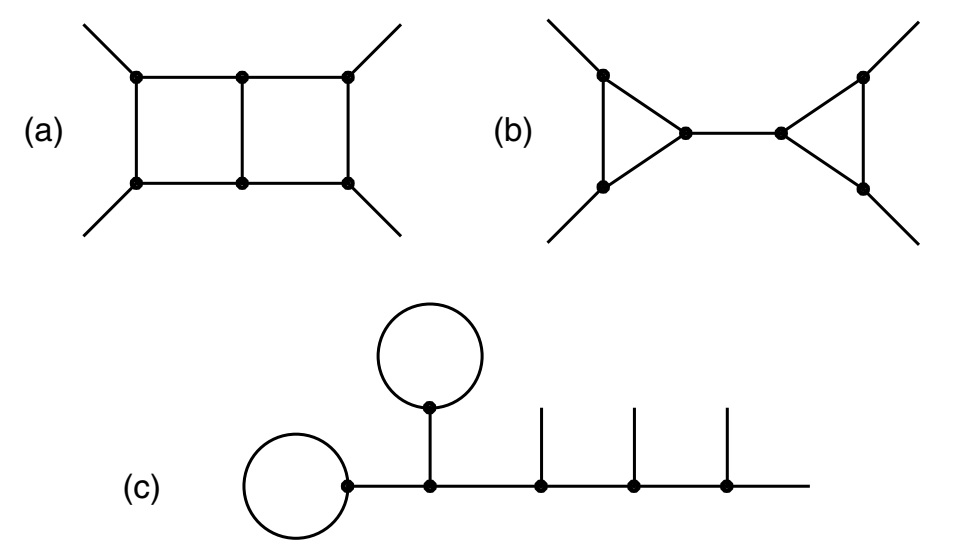
\includegraphics[width=0.6\textwidth,natwidth=667.8,natheight=414.75]{Fig9.4.jpg}
		\caption{有4个算符的亏格2曲面行的一些缝合构造. 每个顶点是一个带有三个孔的球面, 每条内线代表排水管构造, 而每条外线代表一个顶点算符.}\label{Fig9.4}
	\end{center}
\end{figure}

\subsection*{图论分解}

图\ref{Fig9.4}让人联想到费曼图. 我们现在来描述模空间的类费曼图分解. 顶点要比\ref{Fig9.4}复杂得多, 其中可以有任意多条外线以及弦圈中的内部修正. 
这一构造的关键在于让模空间边界的性质变得显然.

陈述如下: 对模空间的积分由费曼图的和给出. 图中的内线传播子代表缝合操作, 要积掉的缝合参量 $q$ 处在某些标准区域中, 例如$|q|<1 $.  
$n$ 点顶角代表有 $n$个小孔的黎曼面. 我们将会看到顶点中的曲面要对模空间的某个内部积分, 并对亏格求和. 
缝合操作是指对要缝合的每个点指定复坐标, 所以顶角的定义必须包含在每个点所做的选择. 在$n$点顶角出现的亏格g的曲面集合记为 $\mathscr{V}_{g,n}$. 
外线代表顶点算符.

\begin{figure}
	\begin{center}
		%width=0.8\textwidth,bb=0 0 343 313
		%1px=0.75pt
		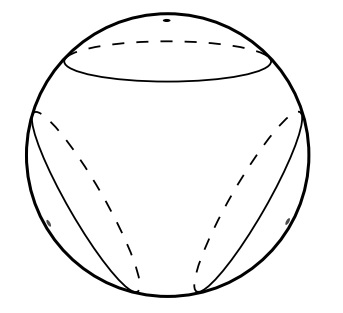
\includegraphics[width=0.4\textwidth,natwidth=257.25,natheight=234.75]{Fig9.5.jpg}\\
		\caption{三线性顶角, 球面上有三个标记点和三个缝合圆.}\label{Fig9.5}
	\end{center}
\end{figure}

我们举例说明这一构造. 从三点顶角 $\mathscr{V}_{0,3}$出发, 如图\ref{Fig9.5}所示, 它是有3个标记点和3个缝合圆的球面. 
在相应点附近的复坐标中, 缝合圆是单位圆. 建立有4个点的球面的步骤: 取两个这样的顶角, 各移掉一个缝合圆的内部, 然后将它们粘在一个圆柱两端; 
这等价于排水管构造. 这对应于图\ref{Fig9.6}a的费曼图; 圆柱的长度为$-\ln |q|$(周长调整为$2\pi$). 对 $|q|<1$ 积分, 
并对其他两个道求和仅给出有四个点的球面的一部分积分区域, 如图\ref{Fig9.6}b所示. 阴影区域被囊括在内, 非阴影区域却消失了.

\begin{figure}[h]
	\begin{center}
		%width=0.8\textwidth,bb=0 0 987 482
		%1px=0.75pt
		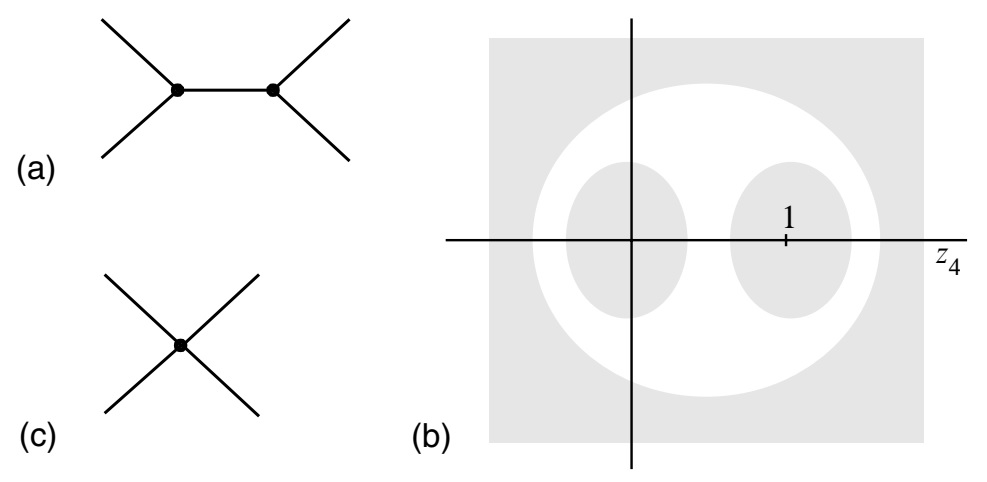
\includegraphics[width=0.8\textwidth,natwidth=740.25,natheight=361.5]{Fig9.6.jpg}\\
		\caption{(a) 构造有四个顶角算符的球面. (b) $z$-平面中被这个图覆盖的区域. (c) 给出正确振幅所需的额外顶角. 对四孔球面在非阴影区域的积分.}\label{Fig9.6}
	\end{center}
\end{figure}

我们来做进一步的解释. 对于三线性顶角, 将点放在球面的 $0,1, \infty$ 处, 并选择坐标系 $z^{(0)}, z^{(1)}$, $z^{(\infty)}$, 
所以三个缝合圆是 $|z^{(0,1, \infty)}|=1$. 这个选择应该在置换顶角的6个Möbius 变换下不变, 这使得顶角是对称的. 存在多个可能的选择, 例如
\begin{equation}
	z^{(0)}=\frac{a z}{z-2}, \quad z^{(1)}=\frac{a(z-1)}{z+1}, \quad z^{(\infty)}=\frac{a}{2 z-1} \:, \label{9.3.6}
\end{equation}
其中$a$为任意常数. 当$a \geq 3$时, 缝合圆不会重合, 保证了对于所有 $q \leq 1$排水管构造都给出好曲面. 读者可以证明, 从两个球面, 
在参量 $q$ 下缝合$z^{(\infty)}$与 $z^{(0)}$ 坐标卡给出了在 $0,1, \frac{1}{2}(1+a^{2}/q)$和 $\frac{1}{2}(1-a^{2}/q)$处有顶角算符的球面. 
在Möbius变换下, 这等价于顶点算符在$0,1, \infty$, 以及
\begin{equation}
	z_{4}=(q-a^{2})^{2}/4 a^{2} q \:. \label{9.3.7}
\end{equation}
随着 $q$跑遍单位圆盘, $z_{4}$ 覆盖了图\ref{Fig9.6}b的外部阴影区域. 置换顶点给出其他两个区域. 
我们可以尝试取更小的$a$, 这样阴影区域会增长, 但它们最终会重合, 并对某些曲面二次计数, 而另一些曲面仍然不会产生. 
它们永远不会精确覆盖整个平面, 所以我们还要添加一个显式的四点顶角 $\mathscr{V}_{0,4}$, 它由有4个标记点的球面给出, 
并对 $z$ 平面的非阴影区域积分. 由于对于$z_{4} $的每个值, 对每个孔的坐标还有一个选择, 这无法完全定义 $\mathscr{V}_{0,4}$. 
以光滑的方式连接阴影区域的边界和非阴影区域的边界. 注意到图\ref{Fig9.6}a的费曼图包含所有渐近区域 $z_{4} \rightarrow 0,1, \infty$, 
而四点顶角只包含非退化曲面. 那么这一极限下的行为显然由$q \rightarrow 0$ 的极限给出: 这是为什么排水管构造有用的原因.

作为一个例子, 将单个顶角的两个圆缝合在一个圆柱的两端, 这给出有一个顶角算符的环面. 这覆盖了环面模空间的$\operatorname{Im} \tau \rightarrow \infty$ 极限, 但内部区域丢失了, 必须通过手加顶角区域 $\mathscr{V}_{1,1}$补回来.

这个构造可以诱导地扩张. 缝合操作总会增加
\begin{equation}
	r = 3g + n - 2  \label{9.3.8}
\end{equation}
个参量. 有三个小孔的原始球面, 顶角$\mathscr{V}_{0,3}$, 有 $r=1$. ``8''操作给出 $r=r_{0}+1$, 而 $\infty$ 操作给出$r=r_{1}+r_{2}$. 
因此, $\mathscr{V}_{0,4}$ 和 $\mathscr{V}_{1,1}$ 均有$r=2$. 已经证明通过 $r$的诱导可以构造出 $\mathscr{V}_{g, n}$, 
因此如同之前宣称的, 覆盖了整个模空间.

下面给出一个更加清晰的构造. 在任意黎曼面上, 存在唯一的最小面积度规, 它的定义是, 最小面积的度规服从使得每个不平庸的闭合曲线的长度至少为 $2 \pi$的约束. 
这个曲面上的每个点至少处在一条饱和测地线上(saturating geodesic), 一条长度精确为$2 \pi$非平庸闭合曲线. 
可以连续变换到其他饱和测地线的饱和测地线不会自相交, 每组同伦等价的饱和测地线构成曲面上的一个环 (拓扑上是圆环). 
不同的环会覆盖整个曲面, 但可能会有重叠. 这种环的高$h$定义为它的两个边界测地线之间的最短距离. 最小面积度规的思想可以扩展至有小孔的曲面, 
方法是, 围绕小孔的圆不是平庸的. 小孔附近的最小面积度规形式为 $\dif z \dif \bar{z} / z \bar{z}$, 一个半径 $2 \pi $ 的半无限长圆柱. 
因此存在两类环, 一类处在曲面内部并且有限, 另一类汇集在小孔处并且半无限长, 终结于曲面内部.

我们现在可以用这种构造描述 $\mathscr{V}_{g, n}$. 取有$n$个小孔的所有黎曼面, 赋予约束, 任何内部环的高度在最小面积度规下小于 $2 \pi $. 
截断半无限长圆柱, 留下长度为$\pi$的存根(stub), 并粘入通常的圆盘中, 在存根的底部插入顶点算符. 有了这些顶角, 费曼图之和会精确地一次性覆盖模空间. 
可以证明, 缝合最小面积曲面仍然会产生最小面积曲面. 高度小于$2 \pi$的环显然包含在顶角中, 高度大于$2 \pi$ 的环会由存根上的缝合算符产生, 
相应高度是存根的$2 \pi$ 加上排水管的$-\ln |q|$; 当对$q$ 积分时, 这从$2 \pi$跑到 $\infty$. 最小长度约束与最大高度保证了简并曲面不会出现在顶角中, 
所以仅当一个或多个$q$趋于零时才会产生, 这正是所要证明的.

\section{共形场论中的缝合与切割} \label{sec:9.4}%{9.4 Sewing and cutting CFTs}



\begin{figure}
	\begin{center}
		%width=0.8\textwidth,bb=0 0 957 668
		%1px=0.75pt
		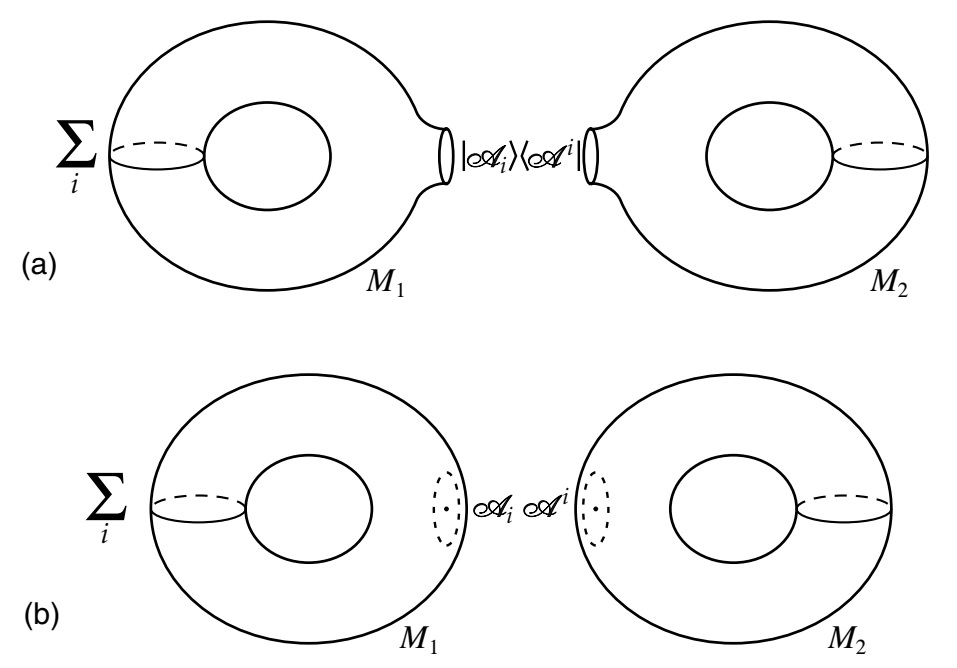
\includegraphics[width=0.8\textwidth,natwidth=717.75,natheight=501]{Fig9.7.jpg}\\
		\caption{(a) 通过插入边界态的一组完备集切开$M$上的路径积分. (b) 每个态被换成了带有定域算符的圆盘.}\label{Fig9.7}
	\end{center}
\end{figure}

通过将低亏格黎曼面缝合在一起, 我们描述了高亏格黎曼面. 利用路径积分的缝合性质, 类似地, 高亏格曲面上的CFT可以与低阶振幅相关联. 这个关系如图\ref{Fig9.7}所示.
为明晰起见, 我们首先讨论 $q=1 $的情况. $M$上的路径积分沿着圆 $|z_{1}|=|z_{2}|=1$剪开, 插入边界态的完备集. 那么每个边界态就被替换成有相应定域算符的圆盘, 
留下未裁剪的世界面 $M_{1}$ 和 $M_{2}$. 这个结果的精确形式是
\begin{equation}
	\langle {}_{\cdots 1} {}_{\cdots 2}\rangle_{M} = \sum_{i j}\Bigl \langle {}_{\cdots 1} \mathscr{A}_{i}^{(z_{1})}\Bigr\rangle_{M_{1}} 
	\mathsf{G}^{ij} \Bigl\langle\mathscr{A}_{j}^{(z_{2})} {}_{\cdots 2}\Bigr\rangle_{M_{2}} \:. \label{9.4.1}
\end{equation}
我们允许在$M_{1}$和$M_{2}$上有任意额外的插入 ${}_{\cdots 1}$ 和 ${}_{\cdots 2}$; 它们必须处在圆 $|z_{1}|=1$ 和$|z_{2}|=1$ 外面. 
我们还没有为这组基指定任何特定的正交性; 仍需决定合适的可逆矩阵 $\mathsf{G}^{i j}$. 代替柄, 插入 $\mathscr{A}_{i}$ 和 $\mathscr{A}_{j}$
分别隐含处在 $z_{1}$ 和 $z_{2}$ 坐标系的原点中.

现在, 我们来考察$M_{2}$是球面的情况, 将缝合坐标 $z_{2}$ 记作$u$, ${}_{\cdots 2}$是$z=0$处的定域算符$\mathscr{A}_{k}$. 
我们从排水管构造中有 $z_{1} u=1$, 从球面中有 $z u=1$, 所以我们可以将 $z_{1}=z$ 扩张至整个缝合区域. 
缝合曲面 $M$ 与 $z_{1}=0$处有一额外算符$\mathscr{A}_{k}$ 的 $M_{1}$相同. 那么 \eqref{9.4.1} 变成
\begin{equation}
	\Bigl \langle {}_{\cdots 1} \mathscr{A}_{k}^{(z_{1})}\Bigr\rangle_{M_{1}} = 
	\sum_{i j}\Bigl\langle {}_{\cdots 1} \mathscr{A}_{i}^{(z_{1})}\Bigr\rangle_{M_{1}} \mathsf{G}^{ij} 
	\Bigl\langle\mathscr{A}_{j}^{(u)} \mathscr{A}_{k}^{(z)}\Bigr\rangle_{S_{2}} \:. \label{9.4.2}
\end{equation}
两点函数 $\langle\mathscr{A}_{j}^{(u)} \mathscr{A}_{k}^{(z)}\rangle_{S_{2}}$ 正是内积 $\lAngle j \vert k\rangle=\mathsf{G}_{jk}$. 
那么\eqref{9.4.2}暗示了
\begin{equation}
	\mathsf{G}^{ij} \mathscr{G}_{jk} = \delta_{k}^{i} \label{9.4.3}
\end{equation}
或者
\begin{equation}
	\mathsf{G}^{ij} = \mathscr{G}^{ij} \:. \label{9.4.4}
\end{equation}
即, 球面上的两点函数定义的内积正是缝合所需要的. 因此, 针对$M_{2}$是含有一个任意定域算符的球面, 我们导出了\eqref{9.4.1}. 
通过态-算符同构, 任何边界态可以以这种方式获得. 既然路径积分是平庸的, 这个结果只依赖缝合区域, 但与曲面的其余区域无关, 
所以它对于任意的 $M_{2}$ 和${}_{\cdots 2}$都成立.

用参量 $q$进行缝合与用 $q=1$以及定域坐标 $z_{1}$和 $z_{2}^{\prime}=z_{2} / q $ 进行缝合是等同的. 
因此, 我们就获得了$\mathscr{A}_{j}$在带撇坐标系中的\eqref{9.4.1}, 因而从回到 $z_{2}$的共形变换中获得额外因子,
\begin{equation}
	\mathscr{A}_{j}^{(z_{2}^{\prime})}=q^{h_{j}} \bar{q}^{\tilde{h}_{j}} \mathscr{A}_{j}^{(z_{2})} \:. \label{9.4.5}
\end{equation}
这个结果是
\begin{equation}
	\langle {}_{\cdots 1 \cdots 2} \rangle_{M} = \sum_{ij} q^{h_{j}} \tilde{q}^{\tilde{h}_{j}} 
	\Bigl\langle {}_{\cdots 1} \mathscr{A}_{i}^{(z_{1})}\Bigr\rangle_{M_{1}} \mathscr{G}^{i j} 
	\Bigl\langle\mathscr{A}_{j}^{(z_{2})} {}_{\cdots 2} \Bigr\rangle_{M_{2}} \:, \label{9.4.6}
\end{equation}
其中我们取了关于权重对角的基. 对于`8'操作,  $M$和$M_{0}$上的路径积分以相同方式关联
\begin{equation}
	\langle {}_{\cdots}\rangle_{M}=\sum_{i j} q^{h_{j}} \bar{q}^{\tilde{h}_{j}} \mathscr{G}^{ij} 
	\Bigl\langle {}_{\cdots 1} \mathscr{A}_{i}^{(z_{1})} \mathscr{A}_{j}^{(z_{2})}\Bigr\rangle_{M_{0}} \:. \label{9.4.7}
\end{equation}

再次考察模空间的边界, 它由一个或多个柄的$q \rightarrow 0$给出. 我们看到低权重算符将会控制这个行为. 
\eqref{9.4.6} 与 \eqref{9.4.7} 类似于OPE, 实际上, 当$M_{2}$是球面, 并且 ${}_{\cdots 2}$是一对顶点算符, \eqref{9.4.6}会退化至OPE. 
这个类比从图\ref{Fig9.3}c看是显然的, 它将这个极限表示成了插入了小柄. 缝合关系表明不只算符乘积, 或者一个小柄, 或者我们可以缝合进小圆的任何扰动, 
均等价于定域算符的和. \eqref{9.4.6}是OPE的漂亮推广. 从$M_{1}$的视角来看, 有一份很小的 $M_{2}$ 粘在$z_{1}=0$附近. 
这可以用定域算符 $\mathscr{A}_{i}$展开, 系数函数是 $\langle\mathscr{A}^{i} {}_{\cdots 2}\rangle_{M_{2}}$. 
以 $M_{2}$的视角看, 有一份细小的$M_{1}$ 粘在 $z_{2}=0$附近, 它可以用 $\mathscr{A}^{i}$展开, 
系数函数是 $\langle {}_{\cdots 1} \mathscr{A}_{i}\rangle_{M_{1}}$.

我们已经论证了每个黎曼面可以退化至带3个小孔的球面. 因此, 缝合构造将所有振幅与球面上的三点振幅关联起来, 而它们显然是算符乘积系数: 它们是定义CFT的数据. 
我们会遇到很多CFT之间的等价性——我们已经看到了T对偶, 而玻色化将是另一个值得注意的例子. 缝合构造提供了两个理论是否相等的判据: 
它们的态和恒等OPE之间的一一映射.\footnote{我们应该注意到, 若有多个(2,0)加(0,2)场可以起到$T_{ab}$的作用, 就像\ref{sec:2.5}节中自由场的例子, 必须要指定哪个是能动量张量. 这个选择决定了算符的共形变换, 这会暗中进入缝合操作之中.} 事实上, 我们会在第15章证明, 仅初级场的算符乘积就决定了所有其他场的算符乘积. 

我们来进一步探索这个观点. 我们可以沿着各种不同的曲线剪开一个曲面, 所以为了保证缝合关系, 对于$M$上的期望值总给出相同的结果. 
首先考察剪切曲线$C$上的无穷小变换. 一般使得$M$不变的无穷小变换可以通过对用于缝合的坐标做无穷小变换获得
\begin{subequations} \label{9.4.8}
\begin{align}
		z_{1}^{\prime} &= z_{1} + \sum_{n=-\infty}^{\infty} \epsilon_{n} z_{1}^{n+1}  \:, \label{9.4.8a} \\
		z_{2}^{\prime} &= z_{2} - \sum_{n=-\infty}^{\infty} \epsilon_{-n} q^{-n} z_{2}^{n+1} \:. \label{9.4.8b}
\end{align}
\end{subequations}
那么缝合表达式的差会正比于
\begin{align}
	\mathscr{A}_{i}^{(z_{1}^{\prime})} \mathscr{G}^{ij} \mathscr{A}_{j}^{(z_{2}^{\prime})} - 
	\mathscr{A}_{i}^{(z_{1})} \mathscr{G}^{ij} \mathscr{A}_{j}^{(z_{2})} 
	&= -\sum_{n=-\infty}^{\infty} \epsilon_{n} \Bigl[L_{n} \cdot \mathscr{A}_{i}^{(z_{1})} \mathscr{G}^{ij} \mathscr{A}_{j}^{(z_{2})} \nonumber \\
	&\quad -\mathscr{A}_{i}^{(z_{1})} \mathscr{G}^{ij} L_{-n} \cdot \mathscr{A}_{j}^{(z_{2})}\Bigr]+\text{(反全纯)} \:, \label{9.4.9}
\end{align}
其中我们使用了共形变换\eqref{2.9.6}, 而反全纯代表将 $\epsilon_{n} \rightarrow \epsilon_{n}^{*}$, 并将 $L_{n} \rightarrow \tilde{L}_{n}$. 
通过用来推导\eqref{9.4.4}的讨论可以证明大括号中的量为零. 这相当于说我们可以将定义生成元的围道积分拉过缝合柄; 
从$L_{n}$ 到 $L_{-n}$ 的变化来自于坐标的反转. 所有其他的守恒荷围道积分也可以拉过来.

还有一些曲线的集合无法通过连续变换关联起来. 通过剪切围绕不同对算符的圆, 球面上的四点振幅可写成三点振幅的形式. 不同缝合之间的等价性是OPE结合律的结果, 
见图\ref{Fig2.8}.

另一个例子由环面给出: 通过沿着$A$ 闭链或$B$闭链, 或者任何其他不自交的闭合曲线剪切, 我们可以使环面退化至球面. 
以带有等价关系的平面来讲, 始于 $(\sigma^{1}, \sigma^{2})=(0,0)$的闭合曲线 $C$ 必须结束于等价点
\begin{equation}
	2 \pi(m, n) \:. \label{9.4.10}
\end{equation}
所有 $m$ 和 $n$值相同的曲线可以连续地变换到彼此, 所以我们需要考察沿着 $m$和$n $不同的缝合曲线之间有什么关系. 
可以证明, 对于非平庸的不自交曲线, $m$ 和 $n$ 必须互素, 这暗示了存在整数 $p$ 和$q$, 使得 $m p-n q=1$. 那么存在另一个模变换
\begin{equation}
	(\sigma^{1}, \sigma^{2}) = (\sigma^{\prime 1}, \sigma^{\prime 2}) \begin{bmatrix}
		m & n \\
		q & p		
	\end{bmatrix} \:, \label{9.4.11}
\end{equation}
使得曲线 $C$ 回到
\begin{equation}
	(\sigma^{\prime 1}, \sigma^{\prime 2})=2 \pi(1,0) \:, \label{9.4.12}
\end{equation}
这是$A$ 闭链. 所以沿着非平庸不自交曲线剪切等同于在 $\tau $的一个模等价值上沿着 $A$ 闭链剪切. 因此, 缝合构造的相容性就等价于模不变性.

通过连续的两个操作, 每组缝合曲线可以变换到彼此: 球面上的四点结合变换, 以及含有一个顶点算符的环面上的模变换. 图\ref{Fig9.4}使其相当可信. 
例如, 图\ref{Fig9.4}a通过一个结合性条件与图\ref{Fig9.4}b相关. 重复利用结合性可以将缝合带至图\ref{Fig9.4}c的形式, 这时所有圈都表示成了单圈单点函数. 
所以, 它们是定义一个合理的共形场论任意一组算符乘积系数的条件. 这种用来解决对偶约束的程式被称为共形自举(conformal bootstrap). 
仅在引入额外约束的情况下, 这才得以实现. 我们将在第15章进行讨论.

这一节的考察可以扩展至有边界的世界面, 除了退化柄以外, 那里还会有退化带. 相容性条件已经推广至这一情况.

\section{一般的振幅}  \label{sec:9.5}%{9.5 General amplitudes}
我们现在已经集齐了理解一般弦振幅的相容性所需要的所有元素. 

在给定模空间的图形分解后, 缝合理论使得我们可以给出一般弦振幅的图形表示. 首先考察来自排水管构造的传播子. 模 $q$ 的鬼插入是
\begin{equation}
	\oint \frac{\dif z}{2 \pi \mi} \: b_{z_{1} z_{1}} \frac{\partial z_{1}}{\partial q}\biggr|_{z_{2}}=\frac{b_{0}}{q} \:, \label{9.5.1}
\end{equation}
类似地, 对于 $\bar{q}$ 则是 $\tilde{b}_{0} / \bar{q}$. 引入这些插入, 并使用缝合表达式\eqref{9.4.6}, 传播子附带的因子是
\begin{equation}
	\int_{|q|<1} \frac{\dif^{2} q}{q \bar{q}} \: q^{\alpha^{\prime}(k_{i}^{2}+m_{i}^{2})/4} 
	\bar{q}^{\alpha^{\prime}(k_{i}^{2}+\tilde{m}_{i}^{2})/4} \mathscr{G}^{ij} b_{0} \tilde{b}_{0}
	= \frac{8 \pi \delta_{m_{i}^{2}, \tilde{m}_{i}^{2}} \mathscr{G}^{ij} b_{0} \tilde{b}_{0}}{\alpha^{\prime}(k_{i}^{2}+m_{i}^{2}-\mi \epsilon)} \:. \label{9.5.2}
\end{equation}
通过在缝合构造的顶点中出现的曲面上插入顶点算符, 就给出了$n$ 弦耦合
\begin{equation}
	g(i_{1}, \ldots, i_{n}) = \sum_{g} \int_{\mathscr{V}_{g, n}} \dif^{m} t  \:
	\biggl\langle\prod_{k=1}^{m} B_{k} \prod_{l=1}^{n} \hat{\nu}_{i_{l}}\biggr\rangle_{g} \:. \label{9.5.3}
\end{equation}
其中$m=6 g+2 n-6$ 是模的数目. 那么从耦合\eqref{9.5.3}和传播子\eqref{9.5.2}构造出的费曼图重新产生了整个弦振幅. 
指标$i$ 依旧代表每个弦的态和动量. \ref{sec:9.1}节中的树图振幅例证了这一结果.

第一个议题是振幅的有限性. 我们断言, 发散只能来自于空间的边界. 就像各种低阶振幅中发生的那样. 在模的有限值处, 缝合公式给出的是对无限个弦态求和, 
但由于这个求和实质上是一个量子态在一个完备基中的展开, 所以这个求和是收敛的. 实际上, 收敛性仅在幺正CFT中才能得以保证, 
但是, 弦CFT的非幺正部分是相当驯服的. $X^{0}$ CFT 是通过从幺正CFT解析延拓定义的, 而鬼场CFT仅仅生成了Faddeev-Popov行列式, 所以是有限的. 
现在边界作为各种传播子的$q \rightarrow 0$极限变得显然, 而积分\eqref{9.5.2}在前面遇到过数次. 它是经由解析延拓定义的, 给出了普通场论传播子. 
那么唯一的奇异性就是传播子中的极点, 它表示在中间态中产生了在壳粒子. 特别地, 它们是长程而非短程发散. 

另一个议题是幺正性, 对于四点树图振幅, 我们稍详细地探讨了幺正性. 将一般振幅带到费曼图形式, 而不是细致地解出组合学, 
我们就可以引用标准场论中关于图形表示幺正性的结果. 另外, 在\ref{sec:9.1}节末尾例证了对中间态的求和会退化至对物理态的求和, 
这一结果会像场论中那样得以推广. 

作为总结, 弦论中的微扰有限性与幺正性所包含议题表现得容易理解. 再次注意到, 我们没有假定26个平坦维, 而仅是$d$个平坦维加上中心荷为 $26-d$的紧致正范的CFT. 
当然, 对于玻色弦而言, 既然平坦时空不是它的解, 任何对于平坦时空S矩阵幺正性的讨论多少有些形式主义——首先存在快子稳定性问题. 其次还有由圈引入的宇宙学常数问题.

证明弦论的有限性和幺正性的另一方法基于光锥规范. 这一方法也被极大地发展了. 这个规范放弃了协变性, 但它有相当的优势——它使得给出模空间的显式描述变得可能, 
并且振幅可以表示成场论形式, 且哈密顿量关于光锥时间 $x^{+}$是定域的. 通过证明微扰论等价于协变微扰论, 协变性随之建立.

\subsection*{弦发散}


\begin{figure}
	\begin{center}
		%width=0.8\textwidth,bb=0 0 937 514
		%1px=0.75pt
		\includegraphics[width=0.8\textwidth,natwidth=702.75,natheight=385.5]{Fig9.8.jpg}\\
		\caption{(a) 有$n$个顶点算符的环面, 其中$m$个聚在一起. (b) 共形等价的图像: 这$m$个顶点算符处在一个长圆柱的末端. 
		(c) 缝合构造, 表示成有$m{+}1$个顶点算符的球面与有$n{-}m{+}1$个顶点算符的环面的乘积.}\label{Fig9.8}
	\end{center}
\end{figure}

在继续前进之前, 我们对弦发散是长程发散做进一步解释. 考察带有 $n$个顶点算符的一圈振幅, 保持$\tau$不动, 取 $m$ 个算符聚在一起的极限, 如图\ref{Fig9.8}所示. 
弦圈当然包含引力, 当相互作用在时空中聚集时, 这有UV发散. 这个弦振幅中确实有发散, 但它来自于长程时空距离, 而不是短程. 
图\ref{Fig9.8}b给出了一个共形等价描述, 在那里, $m$ 个顶点算符通过一个长圆柱与剩余的环面相连. 剪开圆柱, 并插入态的完备集, 
我们获得通常的表示\eqref{9.5.2}, 而 $q \rightarrow 0$ 变成顶点算符聚合的极限. 所以唯一的奇点是传播子在长程时空的极点. 
共形不变性再次将世界面上的短程变成时空中的长程.

$m=n$和$m=n{-}1$ 的情况会呈现出特殊问题. 当$m=n$时, 这意味着所有顶点算符都聚集在一起, 动量守恒令 $k^{\mu}$为零. 对无质量态, 极点就是 $1/0$, 
由于动量守恒会迫使振幅停留在极点上, 所以解析延拓并没有帮助. 这是一个蝌蚪图, 就像\ref{sec:7.4}节中那样, 解决方案是相同的, 对背景场的修正. 
这里的发散正比于带有一个顶点算符的环面振幅.

另外一个有问题的情况是 $m=n-1$, 这时除了一个顶点算符 $\mathscr{V}_{n}$外, 所有顶点算符都聚集在一起. 
动量守恒要求流经圆柱的动量是 $k^{\mu}=-k_{n}^{\mu}$. 然而, 共形不变性要求$k_{n}^{2}=-m_{n}^{2}$, 所以对于那些$m_{j}^{2}=m_{n}^{2}$的中间态, 
中间态动量被固定在一个极点的顶部, 如图\ref{Fig9.9}所示: 中间传播子是 $1/0$. 只要内线 $j$与外线$n$相同, 发散就会发生. 
解释是相当简单的. 这个圈代表的是对粒子$n$质量的辐射修正. 定义S-矩阵的外动量处在真正的质壳上, 其中包括了辐射修正, 并且这依旧没有这个IR发散. 
注意到, 这里的问题不是圈内的UV发散, 而是带星传播子的IR发散, 并且, 即使质量修正是有限的, 这也会发生. 
解决方案在弦情况是相同的. 出现在顶点算符中的动量必须处在真正的物理质量上; 一般而言, 它们与树图质量并不相同, 
那些质量的平方是 $1 / \alpha^{\prime}$的整数倍. 注意到, 对于特定的无质量场——特别是规范玻色子——规范不变性要求它们在所有阶都是无质量的. 
附带地, 对于有质量态, 质量偏移通常是复的, 这些态是不稳定的, 会衰变到轻弦态.

\begin{figure}
	\begin{center}
		%width=0.8\textwidth,bb=0 0 435 233
		%1px=0.75pt
		\includegraphics[width=0.6\textwidth,natwidth=326.25,natheight=174.75]{Fig9.9.jpg}\\
		\caption{与$m=n{-}1$的情况相应的场论图. 运动学会迫使带星传播子发散. 解决方案是由于圈引起的(有限)质量偏移.}\label{Fig9.9}
	\end{center}
\end{figure}


这里有一个问题. 早先我们研究弦理论的相容性时, 世界面共形不变性要求$\beta$-函数\eqref{3.7.14}为零. 
这些$\beta$-函数不包括高亏格曲面的信息——它们对应的是树级弦场方程. 当我们试图围绕圈修正背景展开时, 会发生什么? 
事实上, 所有问题都迎刃而解了. 图\ref{Fig9.8}中的危险极限不仅给出了发散, 也给出了共形反常. 为了看到这点, 
将这一极限画成\ref{Fig9.3}c中那样, 将一个小柄粘在球上. 这个小柄可以用一系列的定域算符表示, 特别地, 从无质量能级中有
\begin{equation}
	\partial X^{\mu} \bar{\partial} X_{\mu} \frac{\dif q \dif \bar{q}}{q \bar{q}} \:. \label{9.5.4}
\end{equation}
现在通过要求柄的大小大于$a$; 即$|q| \me^{\omega}>a$, 其中球面上的度规是 $\dif z \dif \bar{z} \me^{2 \omega}$,  
以坐标不变的方式剪掉发散. 积分\eqref{9.5.4}的下限给出
\begin{equation}
	-4 \pi \partial X^{\mu} \bar{\partial} X_{\mu} \ln (a \me^{-\omega}) \:. \label{9.5.5}
\end{equation}
因此, 我们度规的Weyl因子有了新的依赖: 这修正了$\sigma$-模型的Weyl反常 $\beta_{\mu v}^{G}$, \eqref{3.7.14}. 
为了获得Weyl不变的理论, 背景必须满足完整的弦圈修正的Weyl不变条件 (或等价的, BRST不变性). 
来自偏移背景的Weyl反常抵消了来自小柄的反常, 这是Fischler-Susskind机制. 从图\ref{Fig9.3}c, 我们可以认为发散和Weyl反常是世界面UV效应, 
它们并非来自于通常的场的短波涨落, 而是来自于非常小的拓扑涨落. 我们应该强调的是, 对于亏格任意的固定黎曼面, 定域结构是不受拓扑影响的; 
产生发散和Weyl反常的是对黎曼面的积分. 

这也可以认为是抵消传播子讨论失效了. 运动学迫使振幅处在极点上, 我们无法用解析延拓去消除BRST变分下可能的表面项. 
事实上, 它们的出现对应于Weyl反常\eqref{9.5.5}. 在被圈修正的背景下, 来自背景偏移的BRST反常抵消了模空间边界产生的BRST反常——将弦的特性组装在一起给出了相容的时空图景.

在弦微扰论中实施这点是相当麻烦的, 但幸运的是, 这很少是必要的. 首先, 在大多数超对称理论中, 背景是不修正的. 
其次, 在弦论中, 对长程物理的分析分成两步是最有效的, 首先用弦论推导出低能有效作用量的形式, 然后再长程时使用这个理论. 
那么, 我们无需在弦论级别上处理IR发散. 在目前的情况下, 蝌蚪图给出了如下的势能项
\begin{equation}
	\delta \bm{S}=-\sum_{\chi} \Lambda_{\chi} \int \dif^{d} x \: (-G)^{1/2} \me^{-\chi \Phi} \:. \label{9.5.6}
\end{equation}
这里 $\Lambda_{\gamma}$ 来自欧拉数, 而作用量对$\Phi$的依赖关系来自于$\me^{\Phi}$是弦耦合. 
在经过一番努力后, 我们可以从弦振幅中抽取出引力子和伸缩子的各个蝌蚪图.

同样的概念扩展至来自质量偏移的顶点算符修正, 以及其他的IR发散, 例如, 含有无质量粒子理论中的遍举振幅(exclusive amplitudes), 由于弦论在长程时会退化到场论, 
这些场论发散也必须出现在相应的弦振幅中. 我们再强调一次, 场论中的UV发散一般指出了理论适用范围的基本限制, IR发散通常意味着提出了错误的问题. 
任何这样的发散, 弦论中的处理方式与场论相同.

我们来回顾一下我们学到了什么. 玻色弦特有的模问题, S-矩阵有限且幺正. 基本机制是模不变性, 它截掉了UV发散但没有破坏时空规范不变性. 
当然, 知道弦理论在围绕平坦时空的弱耦合微扰论中是合理的, 这远远不够. 我们希望知道超出微扰论, 这个理论还是否合理, 并有一些计算非微扰修正的手段. 
另外, 我们希望知道对于时空的短程性质, 弦论意味着什么. 在本章的其余部分, 我们将简要描述在这些方向上的尝试.

\section{弦场论} \label{sec:9.6}%{9.6 String field theory}

比较我们在弦论中使用的方法与构建量子场论的方法是很有趣的. 世界面路径积分类似于对粒子路径求和, 这通常称作一次量子化方案. 另一方面, 在量子场论中, 我们可以以一次量子化的形式发展量子场论, 这时必须要引入相互作用顶角, 即几个粒子汇集的地方. 在弦论中, 第二步是不必要的——不存在特殊点, 对拓扑的求和产生了相互作用. 
然而, 这个结果只是微扰展开, 并且有一些现象不会出现在这个展开中. 在标准模型中, 这包括夸克禁闭以及弱作用的有限温度重子数破坏. 
这里似乎没有什么方式使得它们出现微扰展开的重求和中; 相反, 它们要求对理论的更一般构造.

在上一节中, 我们将弦振幅表示成了传播子和顶角形式, 这很像无限分量场论的微扰论. 
我们是否可以用一个对无限组时空场的积分导出这个形式? 是否存在一些原理, 扩展规范不变性和广义坐标不变性, 来决定理论的形式? 
这是弦场论的主题.

我们从如下的假设出发, 取弦波函数 $\Psi[X]$, 并将其提升至场算符, 或者等价的路径积分变量——这是所谓的二次量子化. 
现在, $\Psi[X]$ 依赖于弦在时空中描述的曲线$X^{\mu}(\sigma)$. 粗略地讲, 在这一构形中产生或湮灭了一个弦. 
然而, 我们需要更精细些, 我们是否应该要求$\Psi$在曲线的再参量化下不变? 以及它是否还依赖于 Polyakov 度规 $g_{ab}$? 
如果我们从理论的BRST形式出发, 引入Faddeev-Popov鬼, 然后二次量子化, 貌似一切都很好. 
从对易关系, $b$ 和 $c$ 互相共轭, 所以如果我们将 $c$ 和$\tilde{c}$ 视为坐标, 波函数是 $\Psi[X, c, \tilde{c}]$, 
那么我们就有对所有这些泛函积分的路径积分
\begin{equation}
	\int[\dif \Psi] \: \exp (\mi S[\Psi]) \:. \label{9.6.1}
\end{equation}
我们先来考察开弦, 描述一个特殊方法. 

什么对称性将约束弦作用量? 从我们对弦顶点算符和空(null)态的研究表明, 我们或许会猜测是对称性
\begin{equation}
	\delta \Psi=Q_{\mathrm{B}} \Lambda \label{9.6.2}
\end{equation}
其中$\Lambda$是任意泛函. 有这个不变性的最简单作用量是
\begin{equation}
	S_{0}=\frac{1}{2}\lAngle\Psi |Q_{\mathrm{B}}| \Psi\rangle \:. \label{9.6.3}
\end{equation}
运动方程就是
\begin{equation}
	Q_{\mathrm{B}} \Psi=0 \:. \label{9.6.4}
\end{equation}

看到其合理性的方法之一是将弦场 $\Psi$ 展成无限多个普通场, 每一个对应弦的内态. 
令 $\Psi_{i}[X^{\prime}, c, \tilde{c}]$ 是除了质心 $x^{\mu} $ 之外所有内部模式波函数的完备基. 那么一般的态可以表述成
\begin{equation}
	\Psi[X, c, \tilde{c}]=\sum_{i} \Phi_{i}(x) \Psi_{i}[X^{\prime}, c, \tilde{c}] \:, \label{9.6.5}
\end{equation}
展开系数是剩余变量 $x^{\mu}$的函数. 弦场的路径积分变成对分量函数路径积分的无限乘积
\begin{equation}
	\int[\dif \Psi] \rightarrow \prod_{i} \int[\dif \Phi_{i}] \:. \label{9.6.6}
\end{equation}
同往常一样, 我们可以从基态泛函 $\Psi_{0}$ 出发, 并用上升算符来建立剩余的态. 例如, 只保留前两级的态
\begin{align}
	\Psi &= \Bigl[\varphi(x) + A_{\mu}(x) \alpha_{-1}^{\mu} + B(x) b_{-1} + C(x) c_{-1} + \varphi^{\prime}(x) c_{0}\nonumber \\
	&\qquad+A_{\mu}^{\prime}(x) \alpha_{-1}^{\mu} c_{0} + B^{\prime}(x) b_{-1} c_{0} + C^{\prime}(x) c_{-1} c_{0} + \cdots\Bigr] 
	\Psi_{0} \:. \label{9.6.7}
\end{align}
这里, $\varphi$ 是快子场, $A_{\mu}$是规范场, 而$B$和$C$是与时空规范对称性对应的Faddeev-Popov鬼场. 
带撇的场总可以规范掉, 或者它是辅助场(即它们满足代数方程而非微分方程, 并且可以被消掉). 
可以验证对称性\eqref{9.6.2}包含 $A_{\mu}$上的普通规范变换, 而作用量对$\varphi$是Klein-Gordon形式, 对于$A_{\mu} $是Maxwell形式. 
因此BRST弦场形式理论对时空规范不变性给出了一个非常紧致的推广.


\begin{figure}[h!]
	\begin{center}
		%width=0.8\textwidth,bb=0 0 840 261
		%1px=0.75pt
		\includegraphics[width=0.6\textwidth,natwidth=630,natheight=195.75]{Fig9.10.jpg}
		\caption{(a) $\Psi_{1} * \Psi_{2}$, $\Psi_{1}$的右半边与$\Psi_{2}$的左半边的卷积. 可以认为这定义了对阴影区域的路径积分, 后面会对这个区域的宽度去趋于零的极限. (b) $\int \Psi$, $\Psi$的右半边和左半边的卷积.}\label{Fig9.10}
	\end{center}
\end{figure}
\vspace*{-0.7cm}

解出相互作用也没有什么问题. 通过图\ref{Fig9.10}a所示的泛函积分定义弦场上的乘积操作 $\Psi_{1} * \Psi_{2}$, 
它由$\Psi_{1}$的右边与 $\Psi_{2}$的左边重合而成. 同时定义 $\int$, 它给出 \ref{Fig9.10}b所示的单个弦波函数右边和左边的重叠. 
为了给出相互作用理论, 给规范变换加上非线性项
\begin{equation}
	\delta \Psi=Q_{\mathrm{B}} \Lambda+g \Psi * \Lambda-g \Lambda * \Psi \:. \label{9.6.8}
\end{equation}
$*$ 乘积是结合的, 通过一个围道讨论可以证明 $Q_{\mathrm{B}}$ 像一个导数那样作用,
\begin{equation}
	Q_{\mathrm{B}}(\Psi_{1} * \Psi_{2})=(Q_{\mathrm{B}} \Psi_{1}) * \Psi_{2}+\Psi_{1} *(Q_{\mathrm{B}} \Psi_{2}) \:. \label{9.6.9}
\end{equation}
从这些可以得出\eqref{9.6.8}是封闭的. 利用轮换性质,
\begin{equation}
	\int \Psi_{1} * \Psi_{2}=\int \Psi_{2} * \Psi_{1} \:, \label{9.6.10}
\end{equation}
我们可以写下不变作用量
\begin{equation}
	S=\frac{1}{2} \int \Psi * Q_{\mathrm{B}} \Psi + \frac{2 g}{3} \int \Psi * \Psi * \Psi \:. \label{9.6.11}
\end{equation}
将其写成CFT的形式通常是有用的, 将 $\Psi$ 替换成与顶点算符 $\mathscr{V} \Psi$对应的半圆盘
\begin{equation}
	S=\frac{1}{2}\langle\mathscr{V}_{\Psi} \,Q_{\mathrm{B}} \cdot \mathscr{V}_{\Psi}\rangle_{D_{2}} + 
	\frac{2 g}{3}\langle\mathscr{V}_{\Psi} \mathscr{V}_{\Psi} \mathscr{V}_{\Psi}\rangle_{D_{2}} \:. \label{9.6.12}
\end{equation}
顶点算符位置和共形坐标系并不像\eqref{9.6.12}中标出的那样, 而是如\ref{Fig9.11}所示. 一个 $z^{2 / 3}$ 映射将三顶角半圆盘调整成圆盘. 
这个作用量通过了一个非常重要的检验. 仅对总 $Q^{g}=3$的插入, 圆盘上的路径积分才是非零的. 物理态的顶点算符都有鬼数1, 所以\eqref{9.6.12}的两项都是非零的. 
既然\eqref{9.6.11}是不变的, 我们预期对于规范场, 它退化至非阿贝尔杨-米尔斯作用量, 而现实也的确如此.


Siegel规范是$b_{0} \Psi=0 $. 在动能作用量中, $Q_{\mathrm{B}}$ 只有 $c_{0} L_{0}$ 项幸存下来. 
既然在分量 $L_{0} \propto p^{2}+m^{2}$, 这类似于熟悉的电动力学协变规范. 传播子
\begin{equation}
	\int_{0}^{\infty} \dif t \: \exp (-t L_{0}) = L_{0}^{-1} \label{9.6.13}
\end{equation}
就是对任意长度的带子积分. 顶点就是图\ref{Fig9.11}b中将楔子移去, 将三个带子的末端插入了一个`$\mathsf{Y}$'中.
已经证明, 这等价于用黎曼面求和描述的开弦理论, 特别地, 这个求和中包含对模空间的完整单覆盖. 
另一方面, 这是不出意料的: 弦场论有时空规范不变性\eqref{9.6.8}, 这使得空(null)态会从S-矩阵中退耦. 
我们已经论证了空态的退耦决定了弦振幅的形式, 这其中包括了模空间单覆盖的要求(否则全导数项会给出空态耦合). 
另一方面, 模空间十分复杂, 只有少数几个有显式描述. 由这个弦场论产生的模空间, 按费曼图的求和且每张图写成对带长度的积分, 
在经由弦场论发现之前, 数学家只稍微提前点发现它们.\footnote{另一个从物理出发对模空间的描述来自光锥规范, 其中模是相互作用时间, 
中间态的动量$p^{+}$, 以及每个闭弦的扭角.}


\begin{figure}[h]
	\begin{center}
		%width=0.8\textwidth,bb=0 0 904 352
		%1px=0.75pt
		\includegraphics[width=0.6\textwidth,natwidth=678,natheight=264]{Fig9.11.jpg}\\
		\caption{弦场作用量的CFT表示: (a) 动能项; (b) 相互作用. 一个$z^{2/3}$共形变化将通常围绕每个顶点算符的半圆转变成楔子的形状.}\label{Fig9.11}
	\end{center}
\end{figure}
\vspace*{-0.7cm}

我们来指出这个场论的一个奇怪特征. 我们已经声明了弦场论覆盖了整个模空间, 但是我们从圆环知道, 即使不存在显式的闭弦场, 这个模空间会包含产生闭弦极点的极限. 
闭弦极点来自于带长趋于零的极限而非趋于无穷的极限.\footnote{由于这个原因, 弦场论的这个形式并不适合我们上一节的目的. 我们需要对顶点加入存根来消除意外的发散, 
然后加入闭弦传播子和顶点来覆盖模空间中被省略的部分.} 精确的陈述是开弦场路径积分生成了开弦论加上闭弦论的振幅(除了根本没有边界的曲面, 开弦无法与这样的曲面耦合). 
在这一方面, 以一种不精确的含义, 闭弦就像是开弦的束缚态.

对于只有闭弦的理论, 我们可以用闭弦场重复上面的步骤, 但这将会有点复杂. 对自由作用量\eqref{9.6.3}, 鬼数就已经无法胜任了: 
为了使得物理态之间的矩阵元不为零, 我们需要一个额外的$c$鬼. 这里有一个补救, 它要求弦场 $\Psi$ 和规范变换 $\Lambda$ 被 $b_{0}-\tilde{b}_{0}$ 和 $L_{0}-\tilde{L}_{0} $湮灭. 那么, 作用量
\begin{equation}
	S_{0}^{\prime}=\frac{1}{2}\lAngle\Psi |(c_{0}-\tilde{c}_{0}) Q_{\mathrm{B}}| \Psi\rangle \label{9.6.14}
\end{equation}
就在 $\delta \Psi=Q_{\mathrm{B}} \Lambda $下不变. 对相互作用理论, 不再存在类似于$*$的可结合乘积, 相应地没有模空间的单覆盖. 
就像上节那样, 为了覆盖模空间, 我们需要加入高阶顶角$\mathscr{V}_{g, n}$, 这样的顶角有更高幂次的场以及内部柄. 
类似于开弦作用量, 相应的作用量可以利用所谓的Batalin-Vilkovisky形式理论从对称性原理中得出. 然后, 规范固定给出了上一节描述的微扰论.

从时空规范对称性导出弦论的推导是极其优雅的, 尤其对于开弦. 在开弦场论中引入闭弦是十分吸引人的. 然而, 尚未知晓弦场论是否是超出微扰论的有用工具. 
在当代基于时空超对称性的非微扰发展中, 弦场论并没有起到什么作用, 而这样的发展将在第14章进行讨论. 
相当有可能的是, 对于``弦论''的非微扰构建, 弦, 或者弦场, 不简单地就是它的正确自由度.

\section{高阶行为} \label{sec:9.7} %{9.7 Large order behavior}

弦微扰论的高阶行为有一个有趣的结果. 我们先从场论出发. 考察积分
\begin{equation}
	\int_{-\infty}^{\infty} \dif y \exp \biggl[-\frac{y^{2}}{2!} - \lambda \frac{y^{3}}{3!}\biggr] = 
	\lambda^{-1} \int_{-\infty}^{\infty} \dif z \exp \biggl[-\frac{1}{\lambda^{2}}\biggl(\frac{z^{2}}{2!}+\frac{z^{3}}{3!}\biggr)\biggr] \:,
	\label{9.7.1}
\end{equation}
其中$z=y \lambda $. 这个积分在 $\lambda \neq 0$时发散, 但我们暂且忽视它, 用 $\lambda$的形式幂级数计算它
\begin{equation}
	\sum_{n=0}^{\infty} \frac{(-\lambda)^{n}}{6^{n} n !} \int_{-\infty}^{\infty} \dif y\: y^{3 n} 
	\exp (-y^{2} / 2) = (2 \pi)^{1 / 2} \sum_{k=0}^{\infty} \lambda^{2 k} C_{2 k} \:, \label{9.7.2}
\end{equation}
其中
\begin{equation}
	C_{2 k}=\frac{2^{k} \Gamma(3 k+1 / 2)}{\pi^{1 / 2} 3^{2 k}(2 k) !} \:. \label{9.7.3}
\end{equation}
这个积分是标量场论的零维极限, 这个标量场论中有一个质量项和立方耦合. $\lambda$的展开可以表示成费曼图, 图的传播子是1, 而顶角是 $-\lambda$. 
这样常数 $C_{2 k}$ 就计数了有$2 k$ 个三点顶角的真空图的总数, 等价地, 是 $k+1$ 个圈的真空图总数, 而每个图被赋予了合适的对称因子. 
例如, 读者可以验证有两个顶角的真空图有两个, 而其对称群的阶分别是8和12, 而 $C_{2}=\frac{5}{24}=\frac{1}{8}+\frac{1}{12}$. 
为了得到高阶行为, 我们使用Stirling近似 $n ! \approx n^{n+1 / 2} \me^{-n}$, 那么
\begin{equation}
	C_{2 k} \approx k^{k} \approx k ! \:, \label{9.7.4}
\end{equation}
其中近似是在相差一个形式为$k^{a}$和$b^{k}$的因子下成立的.

我们还可以引入四次项 $\lambda^{2} y^{4} / 4 !$, 这使得积分收敛. $\lambda$ 的幂次通过要求 $z$的作用量中的所有项均正比于 $\lambda^{-2} $ 决定; 
或者等价地, 所有 $k+1$ 圈真空图被赋予权重$\lambda^{2 k}$. 这个额外项并不会对结果有实质性的改变; 估计\eqref{9.7.4}在一定的精度下依旧是成立的.

当考察场论时, 传播子和顶角变得更加复杂. 然而, 高阶处的主导行为往往来自于对图的计数——除非存在不寻常的IR行为或UV行为, 传播子和顶角通常贡献阶为$b^{k}$的因子. 
级数的形式如下
\begin{equation}
	\sum_{k=0}^{\infty} \lambda^{2 k} k ! f_{2 k} \:, \label{9.7.5}
\end{equation}
其中 $f_{2 k} \approx k^{a} b^{k}$, 它的变化要比 $k !$慢得多. 除非 $f_{2 k}$ 中有出乎意料的抵消, 这会发散. 
对于很小的 $\lambda$, 这会暂时变得很小, 随后像$k!$那样增长. 求和中最小项的阶是
\begin{equation}
	\exp [-O(1 / \lambda^{2})] \:. \label{9.7.6}
\end{equation}
这是微扰论的精度是一个渐近展开的特征. 诚然, 像瞬子或者动力学对称性破缺的效应, 它们在微扰论的所有阶都为零, 这样的效应一般是这一阶的. 
例如, 级数 \eqref{9.7.2}的高阶行为与$z=-2$处的瞬子(稳定点)相关, 瞬子的作用量是 $2 / 3 \lambda^{2}$.

在弦理论中, 模空间的费曼图分解使得我们完全有可能构建出相同的约束. 对于形为\eqref{9.7.5}的级数, 若 $f_{2 k}$ 正定且有下界 $b^{k}$, 这已经被显式地证明了. 
因此, 这个级数是发散的, 甚至不是 Borel 可求和的. Borel求和将级数\eqref{9.7.5}重写为对另一个更收敛级数的Laplace变换
\begin{equation}
	\int_{0}^{\infty} \dif t\: \exp (-t) \sum_{k=0}^{\infty}(t \lambda^{2})^{k} f_{2 k} \:. \label{9.7.7}
\end{equation}
然而, $f_{2 k}$ 的正定性暗示了这个新的求和即使收敛但在正实轴上有极点, 所以这个积分是病态的. 
因此, 我们预期弦理论会有一个有趣的非微扰现象. 这并不奇怪, 因为在低能极限下, 它们退化至非平庸的场论.

估计\eqref{9.7.4}对于闭弦理论是个下界, 这可以通过只保留树图三顶点顶角$\mathscr{V}_{0,3}$获得. 
由于闭弦顶角会从所有亏格的黎曼面处得到修正, 我们会好奇是否微扰论会增长得更快. 看到它确实如此的一个方法是回忆起开弦场论包含所有开弦黎曼面, 
以及至少有一个边界的闭弦黎曼面. 我们来考察只有一个边界的曲面, 以及边界收缩至一个点的模空间区域. 
开弦模空间的极限等于有一个顶点算符的闭曲面的模空间. 可以证明这个区域并不比整个开弦模空间小多少, 所以相同的估计依旧成立. 微扰级数趋于
\begin{equation}
	\sum_{k=0}^{\infty} g_{\mathrm{o}}^{2 k} O(k !)=\sum_{k=0}^{\infty} g_{\mathrm{c}}^{k} O(k !) \:. \label{9.7.8}
\end{equation}
亏格为 $g$ 的项正比于 $g_{\mathrm{c}}^{2 g}$, 它有一个阶为 $(2g)!$的系数. 这要大于场论的$g !$特征, 
这样的特征同时是只从 $\mathscr{V}_{0,3}$ 获得的下界. 显然, 高阶振幅的最大部分被包含在顶角 $\mathscr{V}_{g, n}$ 中并来自于模空间的内部. 
可以预期非微扰效应的量级是
\begin{equation}
	\exp [-O(1/g_{\mathrm{c}})] \:, \label{9.7.9}
\end{equation}
它在弱耦合处远大于场论特征$\exp[-O(1 / g_{\mathrm{c}}^{2})]$ . 高阶行为是在\ref{sec:9.9}节将要讨论的一些简化模型中首先观察到的. 
我们将会在第13章看到, 至少是在某些超弦理论中, 这些效应是与D-膜相关的.


\section{高能和高温} \label{sec:9.8}%{9.8 High energy and high temperature}

为了对弦动力学有更好的理解, 我们可以看一下它在不同极限下的行为. 在这一节, 我们考察弦论的各种高能极限.

\subsection*{硬散射}

再一次考察硬散射行为, 这样的行为是通过对Veneziano振幅和 Virasoro-Shapiro 振幅做 Stirling近似获得的. 回到积分形式\eqref{6.6.5},
\begin{equation}
	\frac{8 \pi \mi g_{\mathrm{c}}^{2}}{\alpha^{\prime}} (2\pi)^{26} \delta^{26}({\textstyle \sum_{i} k_{i}}) 
	\int_{\mathds{C}} \dif^{2} z_{4} \: |z_{4}|^{-\alpha^{\prime}u/2 - 4}|1-z_{4}|^{-\alpha^{\prime} t/2 - 4} \:. \label{9.8.1}
\end{equation}
在$t/s$保持固定, $s \rightarrow \infty$的硬散射区域, 指数很大, 积分由指数的稳定点主导.\footnote{同往常一样, 在$z_{4}\to \infty$时, 
积分发散并通过解析延拓定义. 鞍点近似的合理性可以通过延拓论证.} 当 $s, t, u \gg 1$时, 鞍点是
\begin{equation}
	\frac{\partial}{\partial z_{4}}\Bigl(u \ln |z_{4}|^{2}+t \ln |1-z_{4}|^{2}\Bigr) = 
	\frac{u}{z_{4}} + \frac{t}{z_{4}-1} = 0 \:, \label{9.8.2}
\end{equation}
其解是 $z_{4} = -u/s$; 回忆起 $s+t+u=O(1)$. 那么鞍点近似给出振幅
\begin{equation}
	S \approx \exp [-\alpha^{\prime}(s \ln s + t \ln t + u \ln u) / 2] \:, \label{9.8.3}
\end{equation}
同\eqref{6.6.13}给出的一样.

让我们后退一步, 从$z_{4}$的积分回到对 $X^{\mu} $的路径积分. 它由鞍点主导
\begin{equation}
	X_{\mathrm{cl}}^{\mu}(\sigma) = \mi \sum_{i} k_{i}^{\mu} G^{\prime}(\sigma, \sigma_{i}) \:, \label{9.8.4}
\end{equation}
其中$\sigma_{i}$ 是顶点算符位置. 回忆格林函数正比于$\alpha^{\prime}$. 在高能, 散射区域的尺寸随着能量线性增长, $\delta X \approx \alpha^{\prime} k$. 
在场论中, 高能硬散射通过不确定原理探测小距离, $\delta X \approx 1 / k$. 在弦论中, 当超过弦标度之后就不是这样的情况. 
在弦微扰论中表现为不可能探测小于这个标度的距离, 这给出这样的概念, 它是时空中的极限距离. 
紧致化上的有效下界 $R \approx \alpha^{\prime 1/2}$ 也支持这一点. 然而, 我们会在第13章看到, 非微扰弦论中的一些最新发展揭示了更低距离标度的存在.

在弦圈展开的一般阶, 振幅中的主导项是
\begin{equation}
	\exp \Biggl[-\sum_{i<j} k_{i} \cdot k_{j} G^{\prime}(\sigma_{i}, \sigma_{j})\Biggr] \:. \label{9.8.5}
\end{equation}
我们需要找到这个指数的鞍点: 即要针对顶点算符的位置, 又要针对黎曼面的模. 这很像一个静电学问题: 
指数是 $n$ 个带电荷 $k_{i}^{\mu}$ 粒子在黎曼面上的能量, 其中 $\mu$ 标记 $d$ 个不同的静电场, 而$\mu=0$ 在能量上有相反的符号. 
背景电荷密度由于动量守恒为零, 由于 $k_{i}^{2}$在壳且很小, 所以重整化自能可以忽略. 相当显著的是, 在每一个亏格 都会发现可能的鞍点. 考察黎曼面
\begin{equation}
	z_{2}^{N} = \frac{(z_{1}-a_{1})(z_{1}-a_{2})}{(z_{1}-a_{3})(z_{1}-a_{4})} \:. \label{9.8.6}
\end{equation}
同超几何曲线\eqref{9.2.9}一样, 它是$S_{2} \times S_{2}$的子空间. 它可以视为$N$面在割线处粘在一起, 并有亏格 $N{-}1$. 
对于四点振幅, 如果电荷处在割线$a_{i}$处, 振幅相对它们的位置是稳定的——曲面在这些点是``垂直''的, $\partial z_{2} / \partial z_{1}=\infty$, 
而对称性 $z_{2} \to \exp (2 \pi \mi / N) z_{2}$ 要求梯度的垂直分量为零. 相对于位置$a_{i}$它依旧是极值, 但这是很容易的: 
电场与球面上电荷在$z=a_{i}$处的电场相同, 不同之处在于它分成了$N$个分支面. 因此, 能量是$N \cdot N^{-2}=N^{-1}$乘以球面上的能量, 
其中的三个位置可以被Möbius变换固定到$0,1,\infty$, 而第四个由球面上的条件\eqref{9.8.2}给出. 因此在亏格 $g$,
\begin{equation}
	S_{g} \approx \exp [-\alpha^{\prime}(s \ln s + t \ln t + u \ln u) / 2(g+1)] \:. \label{9.8.7}
\end{equation}
经过额外的努力, 可以引入鞍点附近的高斯涨落, 这决定了$S_{g}$的系数. 对于$N$-分支的鞍点, $X_{\mathrm{cl}}^{\mu}$ 只需除以$N=g{+}1$即可.

这里有一个方法可以检验这个结果确实是合理的. 在 $-t / s \ll 1$ 的小角区域, 它变成
\begin{equation}
	\exp [\alpha^{\prime} t \ln s / 2(g+1)] \:. \label{9.8.8}
\end{equation}
现在, $t^{1 / 2}$ 是从入射粒子1到末态粒子3的总转移动量. 在小角区域, 亏格为$g$的散射过程看上去可以分解成 $g{+}1$ 个连续散射. 
每个散射有相同的质心 $s$, 而$t_{i}$ 要满足总转移动量为 $t^{1 / 2}$的约束. 单个散射趋于 $\exp (\alpha^{\prime} t_{i} \ln s / 2)$. 
那么很容易验证取动量传递相等是最有效的, 即$t_{i}^{1/2}=t^{1/2} /(g+1)$, 这给出振幅之积的结果\eqref{9.8.8}. 
这不同于粒子散射, 在那里最有效的散射过程是将动量传递给几个硬散射.

对于弦激发态, 顶点算符的指数行为与快子相同. 那么主导行为为同一个鞍点, 而$X_{\mathrm{cl}}^{\mu}$被代入了顶点算符之中. 
既然除了一个$g+1$因子, 所有态且所有阶的主导鞍点均相同, 在不同态的散射之间存在一个线性关系, 它对于所有亏格都成立, 因而对于精确振幅也很可能是成立的. 
在量子场论中, 高能散射通常会揭示在低能不明显的对称性. 大家广泛认同这里所发现的关系属于同一类.

现在仍然不清楚级数\eqref{9.8.7}的和在什么情况下是有意义的. 对比这一节与上一节的结果是有意义的. 
在这两种情况下, 产生有趣物理结果是模空间内部(与之对照的是, 场论行为是在边界发生的). 
然而高阶行为来自于整个模空间, 特别地, 这个行为由模空间的大体积主导. 而固定亏格处的高能行为由单个点主导.

\subsection*{Regge散射}

对Regge极限的分析也可推广至更高阶. 我们不会做这件事, 但是会对树图Regge物理发展一个有趣的解释. 

对于大多数物理学家, Regge散射没有硬散射那么熟悉. 它是高增速系统的一个温和探针. 
当一个系统被增速后, 时间伸缩子会减慢它的内部过程. 那么当一个高能系统趋于高能时, 我们可以期望看到更多虚自由度.

我们来考察单个弦的量子涨落, 它的平方根意味着基态的尺度. 模展开给出
\begin{align}
	\langle 0 |[X^{1}(\sigma)-x^{1}]^{2}| 0\rangle &= \sum_{n=1}^{\infty} \frac{\alpha^{\prime}}{2 n^{2}}
	\langle 0|(\alpha_{n} \alpha_{-n} + \tilde{\alpha}_{n} \tilde{\alpha}_{-n})| 0\rangle  \nonumber \\
	&= \alpha^{\prime} \sum_{n=1}^{\infty} \frac{1}{n} \:. \label{9.8.9}
\end{align}
这是发散的, 但是没有重要的物理意义. 在时间标度 $\delta \tau$上的测量仅对于频率小于 $\delta \tau^{-1}$的模是敏感的, 
而又有$n \alpha^{\prime-1 / 2}<\delta \tau^{-1}$. 对数发散变成 $\alpha^{\prime} \ln(\alpha^{\prime 1/2} / \delta\tau)$, 而尺寸是它的平方根.

有效尺寸的增长在$t$很小的 Regge 振幅\eqref{6.6.12}中是可以直接观察的
\begin{equation}
	s^{2+\alpha^{\prime}t/2} \frac{\Gamma(-\alpha^{\prime} t/4 - 1)}{\Gamma(\alpha^{\prime} t/4 + 2)} \sim 
	\frac{s^{2}}{t} \exp \biggl[-\frac{q^{2} \alpha^{\prime}}{2} \ln (\alpha^{\prime} s)\biggr] \:, \label{9.8.10}
\end{equation}
其中$q^{2}=-t$是动量转移. 这是一个被形状因子修正的引力振幅$s^{2} / t$, 
形状因子的傅立叶变换对应于一个尺寸为 $(\alpha^{\prime} \ln \alpha^{\prime} s)^{1/2}$的物体. 
从一个弦的视角来看, 另外一个有阶为$\alpha^{\prime} s$的增速, 所以它的内部过程的时间分辨率反比于它, 与这个尺寸的早先估计一致.

对数的平方根是一个增长很慢的函数, 一般不重要, 但需要提醒的是, 这个行为对于黑洞附近的弦非常重要. 
在第14章我们会以一个不同的视角回顾这一点, 弦的概念在增速(boost)很高时揭示出了它们的真实特性.

\subsection*{高温}

弦行为变得有趣的另一个极限是高温. 从配分函数在高权重$h$的一般行为\eqref{7.2.30}, 以及关系 $m^{2}=4(h-1) / \alpha^{\prime}$, 
弦态的密度 $n(m)$ 满足
\begin{equation}
	\int_{0}^{\infty} \dif m\: n(m) \exp (-\alpha^{\prime} \pi m^{2} \ell) \approx \exp (4 \pi / \ell) \:, \label{9.8.11}
\end{equation}
这暗示了 $n(m) \approx \exp (4 \pi m \alpha^{\prime 1/2})$. 那么单个弦的热配分函数就是
\begin{equation}
	\int_{0}^{\infty} \dif m \: \exp (4 \pi m \alpha^{\prime 1/2}) \exp (-m / T) \:. \label{9.8.12}
\end{equation}
因为态密度指数增长, 当温度高于一定值时, 配分函数\eqref{9.8.12}会发散, 这样的温度称为Hagedorn温度
\begin{equation}
	T_{\mathrm{H}}=\frac{1}{4 \pi \alpha^{\prime 1/2}} \:. \label{9.8.13}
\end{equation}
可以对Hagedorn发散有如下理解. 长弦的能量正比于它的长度, 它的熵也是这样, 是广延量. 在低温, 能量主导; 在高温, 熵主导, 并且倾向于产生各种长度的弦. 
在这种弦的系综中, 密度会变大, 并且相互作用在相变点附近会变得重要. 

这一发散表明有一相变. 事实也的确如此, 在高激发强子的态密度有一个类似的增长, 并且从低温强子相到高温夸克-胶子等离子体相有一个相变. 
一个有趣的问题是, Hagedorn发散是否表明在基本弦中有类似夸克-胶子结构, 但这个问题没有明确的答案. 

为了总结, 我们来更加细致地讨论自由弦的配分函数. 在$d$维中, 质量为$m$的实标量场的自由能密度是
\begin{align}
	F(T, m^{2}) &= T \int \frac{\dif^{d-1} \mathbf{k}}{(2 \pi)^{d-1}} \ln [1-\exp(-\omega_{k} / T)] \nonumber \\
				&= - \int_{0}^{\infty} \frac{\dif t}{t}(2 \pi t)^{-d / 2} \sum_{r=1}^{\infty}
				    \exp \biggl(-\frac{m^{2} t}{2}-\frac{r^{2}}{2 T^{2} t}\biggr) \:. \label{9.8.14}
\end{align}
在第二个形式中, 已经可以对弦谱求和. 沿用真空振幅\eqref{7.3.12}和\eqref{7.3.6}的推导, 26平坦维中自由能密度是
\begin{equation}
	F(T)=-\int_{R} \frac{\dif \tau \dif \bar{\tau}}{2 \tau_{2}} (4 \pi^{2} \alpha^{\prime} \tau_{2})^{-13}|\eta(\tau)|^{-48} 
	\sum_{r=1}^{\infty} \exp \biggl(-\frac{r^{2}}{4 \pi T^{2} \alpha^{\prime} \tau_{2}}\biggr) \:. \label{9.8.15}
\end{equation}
这个积分跑遍整个区域
\begin{equation}
	R: \quad \tau_{1} \leq \frac{1}{2}, \qquad |\tau_{2}|>0 \:. \label{9.8.16}
\end{equation}
在 $\tau_{2} \rightarrow 0 $时有一个可能的发散; 当 $\tau$ 的实部为零时, 被积函数为极大值, 所以令 $\tau=\mi \tau_{2}$. 
从模变换\eqref{7.2.44}, $\eta$函数在这一极限下的渐近行为是
\begin{align}
	\eta(\mi \tau_{2}) &= \eta(\mi / \tau_{2}) \tau_{2}^{-1/2} \nonumber \\
	& \approx \exp (-\pi / 12 \tau_{2}) \text { as } \tau_{2} \rightarrow 0 \:. \label{9.8.17}
\end{align}
因此,  $\tau$ 的积分在 $T<T_{\mathrm{H}}$ 时收敛, 在 $T>T_{\mathrm{H}}$时发散.

在场论中, 配分函数由欧几里得路径积分给出, 其时间有周期 $1 / T$. 在弦论中发生了同样的事情. $T$-对偶理应将高温行为与低温行为关联起来. 
事实上, Hagedorn 温度是自对偶值的一半. 定义
\begin{equation}
	\tilde{F}(T)=F(T)+\rho_{0} \:, \label{9.8.18}
\end{equation}
自由能的热部分\eqref{9.8.15} 加上真空部分 \eqref{7.3.6}. 这个路径积分的对数是 $-\tilde{F}(T) / T$, 所以 $T$-对偶暗示了
\begin{equation}
	\frac{1}{T} \tilde{F}(T)=\frac{T}{4 T_{\mathrm{H}}^{2}} \tilde{F}(4 T_{\mathrm{H}}^{2} / T) \:. \label{9.8.19}
\end{equation}
这将Hagedorn温度以下的与Hagedorn温度以上的配分函数关联起来. $T>T_{\mathrm{H}}$时的Hagedorn发散反应了低温理论中的快子发散, 
但是在超弦中有一个类似的形式结果, 而超弦中是没有快子发散的. 如果我们严格地取这个关系, 在$T \rightarrow \infty $时, 我们获得
\begin{equation}
	\tilde{F}(T) \rightarrow \frac{T^{2}}{4 T_{\mathrm{H}}^{2}} \rho_{0} \:. \label{9.8.20}
\end{equation}
如果这衡量了高温自由度数, 那么这是相当少的.  $d$ 维时空中的单个量子场拥有量级为$T^{d}$的自由能, 所以, 弦理论的高温极限看起来就像是两个时空维中的场论. 
这完全不像Hagedorn相变以下指数增长的频谱, 可能是揭示相变性质的一个线索.

\section{低维和非临界弦}  \label{sec:9.9}%{9.9 Low dimensions and noncritical strings}

场论通常会随着时空维数的减少而简化, 而这些低维理论是理解动力学的有用模型. 我们可以尝试在弦论中做同样的事情, 但弦论要求临界维数. 
我们可以紧致化, 但这不会减少自由度的个数: 弦仍然在紧致维中振荡. 然而, 我们遇到过一个相容的背景, 在这个背景场中, 弦实际上在更低维度中运动. 
这是线性伸缩子背景\eqref{3.7.18}
\begin{subequations} \label{9.9.1}
\begin{align}
		G_{\mu \nu}(x) &= \eta_{\mu \nu} \:, \quad B_{\mu \nu}(x) = 0 \:, \quad \Phi(x)=V_{\mu} x^{\mu}  \:, \label{9.9.1a}	\\
		V_{\mu} &= \delta_{\mu}^{1} \biggl(\frac{26-D}{6 \alpha^{\prime}}\biggr)^{1/2} \:. \label{9.9.1b}
\end{align}
\end{subequations}
当$D<26$时, 伸缩子梯度是类空的, 我们已经将其取到1-方向上.

有效弦耦合 $\me^{\Phi}$ 是 $x^{1}$的函数, 在大 $x^{1}$ 处发散. 这使得很难使用弦微扰论, 但幸运的是存在另一个稍微不同的背景, 在这个背景下微扰论是好的. 
将背景\eqref{9.9.1}代入快子作用量\eqref{6.6.16}给出线性快子场方程
\begin{equation}
	-\partial^{\mu} \partial_{\mu} T(x)+2 V^{\mu} \partial_{\mu} T(x)-\frac{4}{\alpha^{\prime}} T(x)=0 \:. \label{9.9.2}
\end{equation}
这是能动张量为线性伸缩子能动张量\eqref{2.5.1}时, 指数顶点算符是Weyl不变的条件. 它的解是
\begin{equation}
	T(x)=\exp (q \cdot x), \quad (q-V)^{2}=\frac{2-D}{6 \alpha^{\prime}} \:. \label{9.9.3}
\end{equation}
如果我们寻求伸缩子这种只依赖于 $x^{1}$的解, 那么
\begin{equation}
	q_{1}=\alpha_{\pm}=\biggl(\frac{26-D}{6 \alpha^{\prime}}\biggr)^{1/2} \pm \biggl(\frac{2-D}{6 \alpha^{\prime}}\biggr)^{1/2} \:. 
	\label{9.9.4}
\end{equation}
当 $D>2$时, 这是复数, 所以快子振荡. 但当 $D \leq 2$时, 会得到实指数 (在临界值 $D=2$ 乘以线性函数). 
当然, 快子场方程有非线性修正. 可以证明, 除了一些相当微妙的原因, 只有$\alpha_{-}$ 会给出不奇异背景外, 这不会影响背景场的定性形式.

对$D \leq 2$, 对于弦基态而言, ``快子''实际上不是一个恰当的术语, 这是因为场是稳定的. 
另外, 当$D \leq 2$时, 实指数 $T(x)=T_{0} \exp (\alpha_{-} x^{1})$ 阻止了向大 $x^{1}$ 区域的传播, 这一区域的耦合是发散的. 
为了看到这点, 考察世界面作用量
\begin{equation}
	S_{\sigma} = \frac{1}{4 \pi \alpha^{\prime}} \int_{M} \dif^{2} \sigma \: g^{1/2} \Bigl[g^{ab} \eta_{\mu\nu} 
	\partial_{a} X^{\mu} \partial_{b} X^{\nu} + \alpha^{\prime} R V_{1} X^{1} + T_{0} \exp (\alpha_{-} X^{1})\Bigr] \:. \label{9.9.5}
\end{equation}
当$x^{1}$很大时, 指数快子会主导线性伸缩子, 而路径积分被压低了, 这对应于弦的由快子背景引起的有效势. 
物理上, 拥有渐近区域$x^{1} \rightarrow-\infty$, 在这一区域耦合趋于零. 向正 $x^{1}$ 传播的弦与其他弦相互作用, 并被有效势反弹回到渐近区域. 
最大有效耦合被势的能量与强度$T_{0}$ 指定. 如图\ref{Fig9.12}, 这一图景有些新奇, 但就寻找可解模型的方面而言, 它是值得追求的. 
一个相当类似的物理的模型, 静态模型, 在揭开量子场论特性方面扮演了重要角色.

\begin{figure}[h]
	\begin{center}
		%width=0.8\textwidth,bb=0 0 648 567
		%1px=0.75pt
		\includegraphics[width=0.5\textwidth,natwidth=486,natheight=425.25]{Fig9.12.jpg}\\
		\caption{背景有伸缩子和快子的时空. 越往右相互作用越强, 但被来自快子背景的一个有效势截断.}\label{Fig9.12}
	\end{center}
\end{figure}
\vspace*{-0.7cm}

当$D>2$ 时, 尽管已经论证了快子背景的作用像个势垒, 但它的物理效应并不非常清晰. 
然而, 将注意力集中在 $D \leq 2$ 上有另一个原因, 即这些理论实际上是可解的. 我们先来观察, 当我们量子化弦时, 规范对称性会带走两族振子. 
这使得 $D \leq 2$ 时什么也不会被剩下——只有质心运动, 一个标量.\footnote{对一些特殊的动量, 会发现额外的物理态. 可以把它们解释成弦场论的未破缺对称性, 
并在理论的可解性中可能起到一定作用.} 然而, 直接解这个弦论是相当困难的. 首先, 必须要计算作用量为\eqref{9.9.5}的世界面路径积分. 
由于指数快子场, 这不再是自由理论. 它被称为刘维尔场论. 它是经典可积的, 再经过一些努力后, 可以定出一些量子振幅. 
然而, 为了解出弦理论, 我们需要在黎曼面模空间的每个亏格上积这个结果; 我们已经看到这是一个紧致空间. 
相当显著的是, 通过相当不同的方法, 直至所有阶的振幅已被确定下来. 为了描述这个方法, 我们必须先引入另一个概念.

\subsection*{非临界弦}

考察这样的一个统计力学系统: 它由对 $d$ 维欧几里得空间中的二维曲面求和定义. 我们同时假定曲面有一些可以解释为长度测度的内部自由度. 
描述这个系统的自然场是嵌入$X^{\mu}(\sigma)$ 与度规 $g_{a b}(\sigma)$. 然而, 没有什么理由将长度扔出这个问题——即, 理论不一定是Weyl不变的. 
因而, 这被称为非临界弦. 这个系统的最低维作用量是有额外世界面常数项的Polyakov作用量, 这样的项在临界弦中会被Weyl不变性所禁止
\begin{equation}
	S=\frac{1}{4 \pi \alpha^{\prime}} \int_{M} \dif^{2} \sigma \: g^{1/2} 
	\Bigl(g^{ab} \partial_{a} X^{\mu} \partial_{b} X_{\mu}+\mu\Bigr) \:. \label{9.9.6}
\end{equation}

没有Weyl不变性, 我们可以用diff不变性部分地确定度规, 但会剩余一个自由度:
\begin{equation}
	g_{ab}(\sigma)=\exp (2 \phi(\sigma)) \hat{g}_{ab}(\sigma) \:, \label{9.9.7}
\end{equation}
其中 $\hat{g}_{ab}$是规范选择, 而度规的标度$\phi$仍然要做路径积分. 这一个规范固定的 Faddeev-Popov行列式与\eqref{3.4.19}相同, 
Weyl固定对后者的贡献是平庸的. 代入度规\eqref{9.9.7}, 曲率是
\begin{equation}
	g^{1/2} R = \hat{g}^{1/2}\Bigl(\hat{R}-2 \hat{\nabla}^{2} \phi\Bigr) \:, \label{9.9.8}
\end{equation}
扔掉场无关项, 这个作用量加上Faddeev-Popov行列式变成
\begin{equation}
	S=\frac{1}{4 \pi \alpha^{\prime}} \int_{M} \dif^{2} \sigma \: \hat{g}^{1/2} \biggl[\hat{g}^{ab} \partial_{a} X^{\mu} \partial_{b} X_{\mu}+\mu \exp 2 \phi + \frac{13 \alpha^{\prime}}{3}\Bigl(\hat{g}^{ab} \partial_{a} \phi \partial_{b} \phi+\hat{R} \phi\Bigr)\biggr]\:.
	\label{9.9.9}
\end{equation}
注意到,  Faddeev-Popov行列式为$\phi$提供了动能项. 与伸缩子-快子作用量\eqref{9.9.5}相比, 我们看到一个显著的相似之处. 
如果我们令 $d=D-1$, 并将新的场 $\phi$ 解释成 $x^{1}$, 并且在作用量\eqref{9.9.5}中重命名 $g_{a b} \to \hat{g}_{a b}$, 那么相同的项都会出现. 
一些系数会有些不同——不存在$\phi$的重标度使得它们均一致——但事实上, 我们声称它们是同一个场论. 
关键在于, 定义临界弦路径积分\eqref{9.9.5}时是将 $\hat{g}_{ab}$ 用作度规, 而非临界弦\eqref{9.9.9}用的是 $\exp (2 \phi) \hat{g}_{a b} $. 
对测度的Weyl变换的一个小心处理可以将一个转换成另一个. 要理解这点, 注意到, 只有整个度规\eqref{9.9.7}出现在临界弦的定义中, 所以在变换
\begin{subequations} \label{9.9.10}
\begin{align}
		\hat{g}_{a b}(\sigma)  &\rightarrow \exp (2 \omega(\sigma)) \hat{g}_{a b}(\sigma) \:,  \label{9.9.10a}\\
		\phi(\sigma) &\rightarrow \phi(\sigma)-\omega(\sigma) \:, \label{9.9.10b}
\end{align}
\end{subequations}
所有量都是不变的. 因此非临界弦获得了Weyl不变性, 而这足以固定自由参量 $\mu$以外的各种系数.

Weyl不变的理论和非Weyl不变的理论可以等价, 这看起来很奇怪. 关键在于, 在场论中, 如果我们同时增加仅用来固定规范的场, 我们总可以增添额外的``假''规范对称性. 
一个规范对称性毕竟只是冗余的描述, 而我们总可以采用更冗余的描述. 对于对称性\eqref{9.9.10}, 我们显然可以仅抵消场$\phi$的Weyl对称性. 
但对于一般的弦背景(例如平坦空间, 那里嵌入坐标是Weyl不变的), 这是不可能的, 并且Weyl不变性是``真实的''.

在任何情况下, 我们现在到达一个很微妙的境地, 我们可以通过对三角剖分曲面的求和来近似非临界弦, 两个点之间边的数目变成长度的测度. 
这些三角剖分曲面类似于大费曼图, 事实上我们可以找到一个量子系统——矩阵模型, 使得这是一个图展开. 
矩阵模型的场是$N \times N$ 矩阵. 取$N \rightarrow \infty$ 并调整其他耦合, (至少对于 $D \leq 2$)存在由光滑大曲面主导的临界点, 
所以我们恢复出了非临界弦. 更进一步, 通过对角化矩阵(至少对于 $D \leq 2$), 矩阵模型是可解的. 
在最后我们会获得一个相当简单的系统(在本征值空间中运动的无相互作用费米子), 折回上面的步骤, 这使得弦振幅的计算可以到任意阶.

我们将细节留在参考文献中. 在任何情况下, 当$D>2$时或者处于超对称理论中, 还没发现它们是有用的. 
然而, 至少我们要提及从这些模型中所学到的重要一课. 微扰论中的$(2g)!$行为, 这最初是在显式矩阵模型中看到的, 并由此论证它在所有弦论中成立. 
在矩阵模型中, 相应的 $\exp [O(-1 / g_{\mathrm{c}})]$ 效应包括费米子在本征值空间中的隧道效应. 
这是否与高维弦论中的 $\exp [O(-1 / g_{\mathrm{c}})]$ 效应有关, 现在仍然不清楚.



\part{超弦理论以及拓展}


\setcounter{section}{0}%更改chapter的计数器值
%\numberwithin{equation}{chapter}%公式计数器从属于节计数器
\numberwithin{equation}{section}%公式计数器从属于节计数器
\numberwithin{figure}{section}%图计数器从属于节计数器
\setcounter{chapter}{9}

\chapter{I型超弦和II型超弦}


\section{超共形代数}

玻色弦中, 质壳条件
\begin{equation}
    p_{\mu}p^{\mu}+m^{2}=0 \label{10.1.1}
\end{equation}
来自于物理态条件
\begin{equation}
    L_{0}\lvert \psi\rangle = 0\: , \label{10.1.2}
\end{equation}
在闭弦中还得加上$ \tilde{L}_{0}\lvert\psi\rangle=0 $. 为了得到费米子, 我们需要\,Dirac\,方程
\begin{equation}
    \mi p_{\mu} \Gamma^{\mu}+m=0\:. \label{10.1.3}
\end{equation}

在玻色弦中, $L_{0} $和$ \tilde{L}_{0} $是能动量张量$(T_{B},\tilde{T}_{B})$的质心模. 现在我们要引入新的守恒量$ T_{F} $和$ \tilde{T}_{F} $, 使得它们的质心模给出\,Dirac\,方程. 注意到, 时空动量$ p^{\mu} $是世界面流$(\partial X^{\mu},\bar{\partial}X^{\mu} )$的质心模, 我们现在期待代数满足
\begin{equation}
    \{\Gamma^{\mu},\Gamma^{\nu}\}=2\eta^{\mu\nu} \:, \label{10.1.4}
\end{equation}
的 $\Gamma$ 矩阵是反对易世界面场$ \psi^{\mu} $的质心模.

现在来考察世界面作用量
\begin{equation}
    S=\frac{1}{4\uppi}\int\dif^{2}z \:
    \left(
    \frac{2}{\alpha^{\prime}}\partial X^{\mu}\bar{\partial}X_{\mu} +\psi^{\mu}\bar{\partial}\psi_{\mu}
    +\tilde{\psi}^{\mu}\partial\tilde{\psi}_{\mu}
    \right)\:.\label{10.1.5}
\end{equation}
$XX $的OPE是
\begin{equation}
    X^{\mu}(z,\bar{z})X^{\nu}(0,0)\sim -\frac{\alpha^{\prime}}{2}\eta^{\mu\nu}\ln\lvert z\rvert^{2}\:.\label{10.1.6}
\end{equation}
$\psi $和$ \tilde{\psi} $分别是全纯和反全纯的, 它们的\,OPE\,是
\begin{equation}
    \psi^{\mu}(z)\psi^{\nu}(0)\sim\frac{\eta^{\mu\nu}}{z}\:,\qquad
     \tilde{\psi}^{\mu}(\bar{z})\tilde{\psi}^{\nu}(0)\sim\frac{\eta^{\mu\nu}}{\bar{z}}\: \label{10.1.7}
\end{equation}
{\emph{世界面超流}}是
\begin{equation}
    T_{F}(z)=\mi(2/\alpha^{\prime})^{1/2}\psi^{\mu}(z)\partial X_{\mu}(z)\:,\qquad
     \tilde{T}_{F}(\bar{z})=\mi(2/\alpha^{\prime})^{1/2}\tilde{\psi}^{\mu}(\bar{z})\bar{\partial} X_{\mu}(\bar{z})
     \:.\label{10.1.8}
\end{equation}

这给出希望的结果: $\psi_{0}^{\mu} $和$ \tilde{\psi}_{0}^{\mu} $模将满足\,Gamma\,矩阵代数, 而$ T_{F} $和$ \tilde{T}_{F} $的质心模有\,Dirac\,算符的形式. 

从\,OPE\,和\,Ward\,恒等式可以得出: 流
\begin{equation}
    j^{\eta}(z)=\eta(z)T_{F}(z)\:, \qquad
    \tilde{\jmath}(\bar{z})=\bar{\eta}(\bar{z}) \tilde{T}_{F}(\bar{z}) \label{10.1.9}
\end{equation}
生成了{\emph{超共形变换}}
\begin{subequations}
\begin{align}
     \epsilon^{-1}(2/\alpha^{\prime})^{1/2}\delta X^{\mu}(z,\bar{z}) &= \eta(z)\psi^{\mu}(z) + \eta(z)^{\ast} \tilde{\psi}^{\mu}(\bar{z})\:, \label{10.1.10a} \\
      \epsilon^{-1}(2/\alpha^{\prime})^{1/2}\delta \psi^{\mu}(z) &= -\eta(z)\partial X^{\mu}(z) \:, \label{10.1.10b}  \\
      \epsilon^{-1}(2/\alpha^{\prime})^{1/2}\delta\tilde{\psi}^{\mu}(\bar{z}) &=-\eta(z)^{\ast}\bar{\partial} X^{\mu}(\bar{z}) \:. \label{10.1.10c}
\end{align}
\end{subequations}
这个变换将对易场$ X^{\mu} $和反对易场$ \psi^{\mu} $和$ \tilde{\psi}^{\mu} $混在了一起, 所以$ \eta(z) $必须是反对易参量. 

\begin{tcolorbox}
\noindent 我们现在来考察$ T_{F},\tilde{T}_{F} $%
与 $X,\psi ,\tilde{\psi} $的\,OPE\,: \\
(1)
\begin{align*}
T_{F}(w)X^{\mu }(z,\bar{z}) &=\mi(2/\alpha ^{\prime })^{1/2}\psi ^{\nu
}(w)\partial X_{\nu }(w)X^{\mu }(z,\bar{z}) \\
&=\mi(2/\alpha ^{\prime })^{1/2}\psi ^{\nu }(w)\partial _{w}\delta _{\nu
}^{\mu }\left( -\frac{\alpha ^{\prime }}{2}\ln \lvert z-w\rvert
^{2}\right)  \\
&=-\mi\left( \alpha ^{\prime }/2\right) ^{1/2}\frac{\psi ^{\mu }(w)}{w-z}
\end{align*}%
类似地可以得到\[
\tilde{T}_{F}(\bar{w})X^{\mu }(z,\bar{z})=-\mi\left( \alpha ^{\prime
}/2\right) ^{1/2}\frac{\tilde{\psi}^{\mu }(\bar{w})}{\bar{w}-\bar{z}}
\]%
利用Ward恒等式\[
\frac{1}{\mi\epsilon }\delta \mathscr{A}(z,\bar{z})=\operatorname{Res}_{w\rightarrow z}j(w)\mathscr{A}(z,%
\bar{z})+\overline{\operatorname{Res}}_{\bar{w}\rightarrow \bar{z}}\tilde{\jmath}(\bar{w})\mathscr{A}(z,\bar{z}%
)
\]%
得到\begin{align*}
\frac{1}{\mi\epsilon }\delta X(z,\bar{z}) &=\eta (z)\left( -\mi\left( \alpha
^{\prime }/2\right) ^{1/2}\psi ^{\mu }(z)\right) +\eta (z)^{\ast }\left(
-\mi\left( \alpha ^{\prime }/2\right) ^{1/2}\tilde{\psi}^{\mu }(\bar{z}%
)\right)  \\
\epsilon ^{-1}\left( 2/\alpha ^{\prime }\right) ^{1/2}\delta X(z,\bar{z})
&=\eta (z)\psi ^{\mu }(z)+\eta (z)^{\ast }\tilde{\psi}^{\mu }(\bar{z})
\end{align*}%
(2)%
\begin{align*}
T_{F}(w)\psi ^{\mu }(z) &=\mi(2/\alpha ^{\prime })^{1/2}\psi ^{\nu
}(w)\partial X_{\nu }(w)\psi ^{\mu }(z) \\
&=\mi(2/\alpha ^{\prime })^{1/2}\frac{\eta ^{\mu \nu }}{w-z}\partial X_{\nu
}(w) \\
&=\mi(2/\alpha ^{\prime })^{1/2}\frac{\partial X^{\mu }(w)}{w-z}
\end{align*}%
利用Ward恒等式得到\begin{align*}
\frac{1}{i\epsilon }\delta \psi ^{\mu }(z) &=\eta (z)\left( \mi(2/\alpha
^{\prime })^{1/2}\partial X^{\mu }(z)\right)  \\
\epsilon ^{-1}(\alpha ^{\prime }/2)^{1/2}\delta \psi ^{\mu }(z) &=-\eta
(z)\partial X^{\mu }(z)
\end{align*}%
(3) 类似地, 就得到(\ref{10.1.10c})
\end{tcolorbox}

两个超共形变换的对易子是共形变换,
\begin{equation}
    \delta_{\eta_{1}}\delta_{\eta_{2}}-\delta_{\eta_{2}}\delta_{\eta_{1}}=\delta_{v}\:,\qquad
    v(z)= -2\eta_{1}(z)\eta_{2}(z) \:, \label{10.1.11}
\end{equation}
类似地, 共形变换和超共形变换的对易子是超共形变换.
\begin{tcolorbox}[breakable]
首先对$ X $验证(\ref{10.1.11}), 可知
\begin{align*}
    \delta_{\eta_{1}}\delta_{\eta_{2}}X &=  (\alpha^{\prime}/2)^{1/2}
    \delta_{\eta_{1}}(\eta_{2}(z)\psi^{\mu}(z) + \eta_{2}(z)^{\ast} \tilde{\psi}^{\mu}(\bar{z})) \\
    &=-(\alpha^{\prime}/2)^{1/2} (2/\alpha^{\prime})^{1/2}
    (\eta_{2}(z)\eta_{1}(z)\partial X^{\mu}(z) + \eta_{2}(z)^{\ast} \eta_{1}(z)^{\ast}\bar{\partial}X^{\mu}(\bar{z}))  \\
    &=
    \eta_{1}(z)\eta_{2}(z)\partial X^{\mu}(z) +
    \eta_{1}(z)^{\ast} \eta_{2}(z)^{\ast}\bar{\partial}X^{\mu}(\bar{z})
\end{align*}
所以
\begin{equation*}
    [\delta_{\eta_{1}},\delta_{\eta_{2}}]X= 
     2\eta_{1}\eta_{2}\partial X^{\mu} + 2\eta_{1}^{\ast} \eta_{2}^{\ast}\bar{\partial}X^{\mu}
     =\delta_{v}X
\end{equation*}
参看(\textcolor{red}{2.4.7}).

接下来对$ \psi $验证(\ref{10.1.11}),
可知\begin{align*}
\delta _{\eta _{1}}\delta _{\eta _{2}}\psi ^{\mu } &=-\delta _{\eta
_{1}}\left( \eta _{2}(z)\partial X^{\mu }(z)\right) =-\eta _{2}(z)\partial
(\delta _{\eta _{1}}X^{\mu }(z)) \\
&=-\eta _{2}(z)\partial (\eta _{1}(z)\psi ^{\mu }(z)+\eta _{1}(z)^{\ast }%
\tilde{\psi}^{\mu }(\bar{z})) \\
&=-\eta _{2}\eta _{1}\partial \psi ^{\mu }-\eta _{2}(\partial \eta
_{1})\psi ^{\mu }
\end{align*}%
所以\begin{align*}
\lbrack \delta _{\eta _{1}},\delta _{\eta _{2}}]\psi ^{\mu } &=-\eta
_{2}\eta _{1}\partial \psi ^{\mu }-\eta _{2}(\partial \eta _{1})\psi ^{\mu
}+\eta _{1}\eta _{2}\partial \psi ^{\mu }+\eta _{1}(\partial \eta _{2})\psi
^{\mu } \\
&=2\eta _{1}\eta _{2}\partial \psi ^{\mu }+\partial (\eta _{1}\eta
_{2})\psi ^{\mu }
\end{align*}%
由于$\psi $是$(\frac{1}{2},0)$场, 这正是$\delta _{v}\psi $, 实际是对于权重为$(h,0)$的primary场$\mathcal{O}$, 根据(2.4.16)%
\[
T(z)\mathcal{O}(w,\bar{w})=\frac{h}{(z-w)^{2}}\mathcal{O}(w,\bar{w})+\frac{1}{(z-w)}\partial \mathcal{O}(w,%
\bar{w})+\cdots \text{ ,}
\]%
那么Ward恒等式给出\begin{align*}
\frac{1}{\mi }\delta _{v}\mathcal{O} &=\operatorname{Res}_{z\to w}\Bigl(\mi v(z)T(z)\mathcal{O}(w,%
\bar{w})\Bigr) \\
\delta _{v}\mathcal{O} &=-\left( h(\partial v)\mathcal{O}+v\partial \mathcal{O}\right)
\end{align*}
对于$ \tilde{\psi} $类似.

现在来考察共形变换和超共形变换的对易子, 首先是$X$%
\begin{align*}
\delta _{\eta }\delta _{v}X &=\delta _{\eta }(-v\partial X-v^{\ast }\bar{%
\partial}X)=-v\partial \left( \delta _{\eta }X\right) -v^{\ast }\bar{\partial%
}\left( \delta _{\eta }X\right)  \\
&=-v\partial \left( \eta \psi +\eta ^{\ast }\tilde{\psi}\right) -v^{\ast }%
\bar{\partial}\left( \eta \psi +\eta ^{\ast }\tilde{\psi}\right)  \\
&=-v(\partial \eta )\psi -v\eta \partial \psi -v^{\ast }(\partial \eta
)^{\ast }\tilde{\psi}-v^{\ast }\eta ^{\ast }\bar{\partial}\tilde{\psi}
\end{align*}%
而
\begin{align*}
\delta _{v}\delta _{\eta }X &=\delta _{v}(\eta \psi +\eta ^{\ast }\tilde{%
\psi})=\eta \left( -v\partial \psi -\tfrac{1}{2}\left( \partial v\right) \psi
\right) +\eta ^{\ast }\left( -v^{\ast }\bar{\partial}\tilde{\psi}-\tfrac{1}{2}%
\left( \partial v\right) ^{\ast }\tilde{\psi}\right)
\end{align*}%
所以
\begin{align*}
\lbrack \delta _{\eta },\delta _{v}]X &=-v(\partial \eta )\psi -v\eta
\partial \psi -v^{\ast }(\partial \eta )^{\ast }\tilde{\psi}-v^{\ast }\eta
^{\ast }\bar{\partial}\tilde{\psi} \\
&\quad+\eta v\partial \psi +\tfrac{1}{2}\eta \left( \partial v\right) \psi +\eta
^{\ast }v^{\ast }\bar{\partial}\tilde{\psi}+\tfrac{1}{2}\eta ^{\ast }\left(
\partial v\right) ^{\ast }\tilde{\psi} \\
&=-v(\partial \eta )\psi -v^{\ast }(\partial \eta )^{\ast }\tilde{\psi}+%
\tfrac{1}{2}\eta \left( \partial v\right) \psi +\tfrac{1}{2}\eta ^{\ast
}\left( \partial v\right) ^{\ast }\tilde{\psi} \\
&=\delta _{\eta ^{\prime }}X
\end{align*}%
其中\[
\eta ^{\prime }=-v\partial \eta +\tfrac{1}{2}\eta \partial v
\]%
对于$\psi $%
\begin{align*}
\delta _{\eta }\delta _{v}\psi  &=\delta _{\eta }\left( -v\partial \psi +%
\tfrac{1}{2}(\partial v)\psi \right) =-v\partial \left( \delta _{\eta }\psi
\right) +\tfrac{1}{2}(\partial v)\delta _{\eta }\psi  \\
&=-v\partial \left( \eta \partial X\right) -\frac{1}{2}(\partial v)\eta
\partial X \\
&=-v\eta \partial ^{2}X-v\partial \eta \partial X-\tfrac{1}{2}(\partial
v)\eta \partial X
\end{align*}%
而\begin{align*}
\delta _{v}\delta _{\eta }\psi  &=\delta _{v}(\eta \partial X)=\eta
\partial (\delta _{v}X)=\eta \partial (-v\partial X-v^{\ast }\bar{\partial}X)
\\
&=-\eta \partial v\partial X-\eta v\partial ^{2}X
\end{align*}%
所以\begin{align*}
\lbrack \delta _{\eta },\delta _{v}]\psi  &=-v\eta \partial ^{2}X-v\partial
\eta \partial X-\tfrac{1}{2}(\partial v)\eta \partial X+\eta \partial
v\partial X+\eta v\partial ^{2}X \\
&=-v\partial \eta \partial X+\tfrac{1}{2}(\partial v)\eta \partial X \\
&=\delta _{\eta ^{\prime }}X
\end{align*}%
对于$\tilde{\psi}$类似.
\end{tcolorbox}
从上面我们看到共形变换加上超共形变换封闭, 它们合起来构成了{\emph{超共形代数}}. 以流的形式, 这意味着$T_{F}$与$T_{B}$的OPE封闭, 不过这时的$T_{B}$要加入费米子部分
\begin{equation}
    T_{B}=-\frac{1}{\alpha^{\prime}}\partial X^{\mu}\partial X_{\mu}-\frac{1}{2}\psi^{\mu}\partial\psi_{\mu}
\end{equation}
它们的OPE是
\begin{subequations}
\begin{align}
    T_{B}(z)T_{B}(0)&\sim \frac{3D}{4z^{4}}+\frac{2}{z^{2}}T_{B}(0)+\frac{1}{z}\partial T_{B}(0)\:,\label{10.1.13a}\\
    T_{B}(z)T_{F}(0)&\sim \frac{3}{2z^{2}}T_{F}(0)+\frac{1}{z}\partial T_{F}(0)\:,\label{10.1.13b}\\
    T_{F}(z)T_{F}(0)&\sim \frac{D}{z^{3}}+\frac{2}{z}T_{B}(0) \:,\label{10.1.13c}
\end{align}
\end{subequations}
反全纯流有类似的结果. $T_{B}T_{F}$的OPE暗示了$T_{F}$是权重为$(\frac{3}{2},0)$的张量. 每个标量为中性荷贡献1, 而每个旋量为中心荷贡献$\frac{1}{2}$, 所以总的中心荷是
\begin{equation}
    c=(1+\tfrac{1}{2})D=\tfrac{3}{2}D\:.\label{10.1.14}
\end{equation}
同玻色弦一样, $T_{B}$和$T_{F}$是态上的约束代数, 它们会从频谱中移去一些态.

更一般的$N=1$超共形代数是
\begin{subequations}
\begin{align}
    T_{B}(z)T_{B}(0)&\sim \frac{c}{2z^{4}}+\frac{2}{z^{2}}T_{B}(0)+\frac{1}{z}\partial T_{B}(0)\:,\label{10.1.15a}\\
    T_{B}(z)T_{F}(0)&\sim \frac{3}{2z^{2}}T_{F}(0)+\frac{1}{z}\partial T_{F}(0)\:,\label{10.1.15b}\\
    T_{F}(z)T_{F}(0)&\sim \frac{2c}{3z^{3}}+\frac{2}{z}T_{B}(0) \:,\label{10.1.15c}
\end{align}
\end{subequations}

\begin{tcolorbox}[breakable]
对于$T_{B}$, 我们可以将其写成$T_{B}^{X}$与$T_{B}^{\psi }$的和, 关于$T_{B}^{X}$的部分已经在2.2%
节讨论过, 参看\eqref{2.2.11}和\eqref{2.4.22},
现在只需考察$T_{B}^{\psi }$.%
\begin{align*}
T_{B}^{\psi }(z)T_{B}^{\psi }(\omega ) &=\frac{1}{4}:\psi ^{\mu
}(z)\partial _{z}\psi _{\mu }(z)::\psi ^{\nu }(w)\partial _{w}\psi _{\nu
}(w): \\
&=-\frac{1}{4}\frac{\eta ^{\mu \nu }}{z-w}\partial _{z}\partial _{w}\frac{%
\eta _{\mu \nu }}{z-w}+\frac{1}{4}\partial _{w}\frac{\delta _{\nu }^{\mu }}{%
z-w}\partial _{z}\frac{\delta _{\nu }^{\mu }}{z-w} \\
&\quad+\frac{1}{4}\partial _{w}\frac{\delta _{\nu }^{\mu }}{z-w}\partial
_{z}\psi _{\mu }(z)\psi ^{\nu }(w)-\frac{1}{4}\frac{\eta ^{\mu \nu }}{z-w}%
\partial _{z}\psi _{\mu }(z)\partial _{w}\psi _{\nu }(w) \\
&\quad+\frac{1}{4}\partial _{z}\frac{\delta _{\mu }^{\nu }}{z-w}\psi ^{\mu
}(z)\partial _{w}\psi _{v}(w)-\frac{1}{4}\partial _{z}\partial _{w}\frac{%
\eta _{\mu \nu }}{z-w}\psi ^{\mu }(z)\psi ^{\nu }(w) \\
&=\frac{1}{4}\frac{2D}{(z-w)^{4}}+\frac{1}{4}\frac{-D}{(z-w)^{4}}+\frac{1}{4%
}\frac{1}{\left( z-w\right) ^{2}}\partial _{z}\psi ^{\mu }(z)\psi _{\mu }(w)
\\
&\quad-\frac{1}{4}\frac{1}{(z-w)^{2}}\psi ^{\mu }(z)\partial _{w}\psi _{\mu }(w)-%
\frac{1}{4}\frac{1}{z-w}\partial _{z}\psi ^{\mu }(z)\partial _{w}\psi _{\mu
}(w) \\
&\quad-\frac{1}{4}\frac{-2}{(z-w)^{3}}\psi ^{\mu }(z)\psi _{\mu }(w) \\
&=\frac{D}{4(z-w)^{4}}+\frac{1}{4}\frac{1}{\left( z-w\right) ^{2}}\partial
_{w}\psi ^{\mu }(w)\psi _{\mu }(w)+\frac{1}{4}\frac{1}{z-w}\partial
_{w}^{2}\psi ^{\mu }(w)\psi _{\mu }(w) \\
&\quad-\frac{1}{4}\frac{1}{(z-w)^{2}}\psi ^{\mu }(w)\partial _{w}\psi _{\mu }(w)-%
\frac{1}{2}\frac{1}{(z-w)}\partial _{w}\psi ^{\mu }(w)\partial _{w}\psi
_{\mu }(w) \\
&\quad+\frac{1}{2}\frac{1}{(z-w)^{2}}\partial _{w}\psi ^{\mu }\psi _{\mu
} +\frac{1}{4(z-w)}\partial _{w}^{2}\psi ^{\mu }\psi _{\mu } \\
&=\frac{D}{4(z-w)^{4}}-\frac{1}{(z-w)^{2}}\psi _{\mu }\partial _{w}\psi
^{\mu }-\frac{1}{2}\frac{1}{(z-w)}\left( \psi _{\mu }\partial _{w}^{2}\psi
^{\mu }+\partial _{w}\psi ^{\mu }\partial _{w}\psi _{\mu }\right)  \\
&=\frac{D}{4(z-w)^{4}}+\frac{2T_{B}^{\psi }(w)}{(z-w)^{2}}+\frac{\partial
T_{B}^{\psi }(w)}{z-w}
\end{align*}
需要注意的是, 第一个等号后出现负号是因为$ \psi $的反对易性, 同样由于反对易性, 所以$ (z-w)^{-3}\psi^{\mu}(w)\psi_{\mu}(w) $为零, 加上$T_{B}^{X}(x)T_{B}^{X}(w)$的OPE, 我们就给出了(\ref{10.1.13a}).

接下来证明(\ref{10.1.13b})%
\begin{align*}
T_{B}(z)T_{F}(\omega ) &=\left( -\frac{1}{\alpha ^{\prime }}\partial
_{z}X^{\mu }\partial _{z}X_{\mu }-\frac{1}{2}\psi ^{\mu }\partial _{z}\psi
_{\mu }\right) \left( \mi\sqrt{\frac{2}{\alpha ^{\prime }}}\psi ^{\nu
}(w)\partial _{w}X_{\nu }(w)\right)  \\
&=-\mi\sqrt{\frac{2}{\alpha ^{\prime 3}}}2\partial _{z}\partial _{w}\frac{%
-\alpha ^{\prime }}{2}\ln |z-w|^{2}\partial _{z}X_{\mu }\psi ^{\mu }(w) \\
&\quad+\frac{\mi}{2}\sqrt{\frac{2}{\alpha ^{\prime }}}\frac{\eta ^{\mu \nu }}{z-w}%
\partial _{z}\psi _{\mu }\partial _{w}X_{\nu }(w)-\frac{\mi}{2}\sqrt{\frac{2}{%
\alpha ^{\prime }}}\partial _{z}\frac{\delta _{\mu }^{\nu }}{z-w}\psi ^{\mu
}(z)\partial _{w}X_{\nu }(w) \\
&=\mi\sqrt{\frac{2}{\alpha ^{\prime }}}\frac{1}{(z-w)^{2}}\partial _{z}X_{\mu
}\psi ^{\mu }(w)+\frac{\mi}{2}\sqrt{\frac{2}{\alpha ^{\prime }}}\frac{1}{z-w}%
\partial _{z}\psi _{\mu }\partial _{w}X^{\mu }(w) \\
&\quad+\frac{\mi}{2}\sqrt{\frac{2}{\alpha ^{\prime }}}\frac{1}{(z-w)^{2}}\psi
^{\nu }(z)\partial _{w}X_{\mu }(w) \\
&=\frac{3}{2}\mi\sqrt{\frac{2}{\alpha ^{\prime }}}\frac{1}{(z-w)^{2}}\psi
^{\mu }\partial _{w}X_{\mu }(w)+\mi\sqrt{\frac{2}{\alpha ^{\prime }}}\frac{1}{%
z-w}\psi ^{\mu }\partial _{w}^{2}X_{\mu }(w) \\
&\quad\frac{\mi}{2}\sqrt{\frac{2}{\alpha ^{\prime }}}\frac{1}{z-w}\partial
_{w}\psi _{\mu }\partial _{w}X^{\mu }(w)+\frac{\mi}{2}\sqrt{\frac{2}{\alpha
^{\prime }}}\frac{1}{z-w}\partial _{w}\psi ^{\nu }(w)\partial _{w}X_{\mu }(w)\\
&=\frac{3}{2(z-w)^{2}}T_{F}(w)+\frac{\mi}{z-w}\sqrt{\frac{2}{\alpha ^{\prime }%
}}\left( \psi ^{\mu }\partial _{w}^{2}X_{\mu }(w)+\partial _{w}\psi _{\mu
}\partial _{w}X^{\mu }(w)\right)  \\
&=\frac{3}{2(z-w)^{2}}T_{F}(w)+\frac{1}{z-w}\partial T_{F}(w)\text{ ,}
\end{align*}
最后我们来考察$T_{F}(z)T_{F}(w)$
\begin{align*}
T_{F}(z)T_{F}(w) &=-(2/\alpha ^{\prime })\psi ^{\mu }(z)\partial X_{\mu
}(z)\psi ^{\nu }(w)\partial X_{\nu }(w) \\
&=-(2/\alpha ^{\prime })\frac{\eta ^{\mu \nu }}{z-w}\partial _{z}\partial
_{w}[(-\alpha ^{\prime }/2)\eta _{\mu \nu }\ln |z-w|^{2}] \\
&\quad-(2/\alpha ^{\prime })\frac{\eta ^{\mu \nu }}{z-w}\partial X_{\mu
}(z)\partial X_{\nu }(w)\\
&\quad-(2/\alpha ^{\prime })\psi ^{\mu }(z)\psi ^{\nu
}(w)\partial _{z}\partial _{w}[(-\alpha ^{\prime }/2)\eta _{\mu \nu }\ln
|z-w|^{2}] \\
&=\frac{D}{(z-w)^{3}}+\frac{2}{z}T_{B}^{X}(w)+\psi ^{\mu }(z)\psi _{\mu }(w)%
\frac{1}{(z-w)^{2}} \\
&=\frac{D}{(z-w)^{3}}+\frac{2}{z}T_{B}^{X}(w)-\psi _{\mu }(w)\partial
_{w}\psi ^{\mu }(w)\frac{1}{z-w} \\
&=\frac{D}{(z-w)^{3}}+\frac{2}{z}T_{B}(w)
\end{align*}
这就证明了(\ref{10.1.13c})
\end{tcolorbox}

\subsection*{自由SCFT}
反对易$bc$理论加上对易$\beta\gamma$系统会构成自由的SCFT. 二者的权重分别是
\begin{subequations}
\begin{align}
    h_{b}&=\lambda\:,\qquad h_{c}=1-\lambda \:, \label{10.1.16a} \\
    h_{\beta}&=\lambda-\tfrac{1}{2}\:,\qquad h_{\gamma}=\tfrac{3}{2}-\lambda \:. \label{10.1.16b}
\end{align}
\end{subequations}
作用量是
\begin{equation}
    S_{BC}=\frac{1}{2\uppi}\int\dif^{2}z\: (b\bar{\partial}c+\beta\bar{\partial}\gamma)\:, \label{10.1.17}
\end{equation}
而$T_{B}$和$T_{F}$分别是
\begin{subequations}
\begin{align}
    T_{B}&=(\partial b)c-\lambda\partial(bc)+(\partial \beta)\gamma-\frac{1}{2}(2\lambda-1)\partial(\beta\gamma)\:,
    \label{10.1.18a} \\
    T_{F}&=-\frac{1}{2}(\partial \beta)c+ \frac{2\lambda-1}{2}\partial(\beta c)-2b\gamma\:.\label{10.1.18b}
\end{align}
\end{subequations}
中心荷是
\begin{equation}
    [-3(2\lambda-1)^{2}+1]+[3(2\lambda-2)^{2}-1]=9-12\lambda\:.\label{10.1.19}
\end{equation}
当然, 还有相应的反全纯理论.

我们可以预测出超共形鬼有$\lambda=2$, 反对易$(2,0)$鬼$ b $对应的是对易$(2,0)$约束$T_{B}$, 而对易$(\frac{3}{2},0)$鬼$ \beta $对应的是反对易$(\frac{3}{2},0)$约束$T_{F}$. 鬼场中心荷是$-26+11=-15$, 这给出了临界维数
\begin{equation}
    0=\frac{3}{2}D-15 \Rightarrow D=10\:.\label{10.1.20}
\end{equation}
当$\lambda=2$时,
\begin{subequations}
\begin{align}
    T_{B}&=(\partial b)c-2\partial(bc)+(\partial \beta)\gamma-\frac{3}{2}\partial(\beta\gamma)\:,
    \label{10.1.21a} \\
    T_{F}&=(\partial \beta)c+ \frac{3}{2}\beta\partial c - 2b\gamma\:.\label{10.1.21b}
\end{align}
\end{subequations}
 
另一个自由\,SCFT\,是线性伸缩子理论的超对称版. 它依旧有作用量(\ref{10.1.5}), 但
\begin{subequations}
    \begin{align}
        T_{B}(z)&=-\frac{1}{\alpha^{\prime}} \partial X^{\mu}\partial X_{\mu} +V_{\mu}\partial^{2}X^{\mu} -\frac{1}{2}\psi^{\mu}\partial\psi_{\mu} \:,\label{10.1.22a} \\
        T_{F}(z)&= \mi(2/\alpha^{\prime})^{1/2}\psi^{\mu}\partial X_{\mu}-\mi (2\alpha^{\prime})^{1/2}V_{\mu}\partial\psi^{\mu} \:, \label{10.1.22b} 
    \end{align} \label{10.1.22}
\end{subequations}
可以证明它们满足
\begin{equation}
    c=\frac{3}{2}D+6\alpha^{\prime} V^{\mu}V_{\mu}  \label{10.1.23}
\end{equation}
的\,N=1\,代数.

{\Large{\emph{{$\beta\gamma$场的起源}}}}\\

微分同胚不变性(diffeomorphism)带来的冗余给出了$bc$鬼场, 当我们引入超对称性, 定域超对称性带来的冗余就给出了$\beta\gamma$鬼场. 为此我们要恢复作用量(\ref{10.1.5})的微分同胚不变性并使得超对称性定域.
为此我们先恢复世界面的Minkowski特征, 这时作用量变成
\begin{equation*}
    S=-\int\dif^{2}\sigma\:\frac{1}{4\uppi\alpha^{\prime}}(
    \eta^{ab}\,\partial_{a}X^{\mu}\partial_{b}X_{\mu})
    +\frac{1}{4\uppi}(\mi\overline{\psi}^{\mu}\rho^{a}\partial_{a}\Psi_{\mu})\:.
\end{equation*}
其中
\begin{equation*}
    \rho^{0}=\mi\sigma_{2}=
    \left(\begin{array}{cc}
         0&1  \\
         -1&0 
    \end{array}\right) \qquad
    \rho^{1}=\sigma_{1}=
    \left(\begin{array}{cc}
         0&1  \\
         1&0 
    \end{array}\right)
\end{equation*}
$\rho^{a}$是二维的Dirac矩阵, 它满足$\{\rho^{a},\rho^{b}\}=2\eta^{ab}$. 而$\overline{\psi}=\Psi^{\dag}\rho^{0}$, 对于Majorana旋量$\lambda$, $\bar{\lambda}=\lambda^{\mathrm{T}}\rho^{0}$.
\\
很容易验证这个作用量有{\emph{整体}}超对称变换:
\begin{align*}
    \delta_{\epsilon}X^{\mu}&=\mi(\alpha^{\prime}/2)^{1/2}\,\bar{\epsilon}\,\Psi^{\mu} \\
    \delta_{\epsilon}\Psi^{\mu}&=(2\alpha^{\prime})^{-1/2}\rho^{a}\partial_{a}X^{\mu}\epsilon\:, \\
    \delta _{\epsilon }\overline{\psi}^{\mu }&=-(2\alpha ^{\prime })^{-1/2}\bar{\epsilon}\rho ^{a}\partial _{a}X^{\mu }
\end{align*}

所以在这个变换下, 作用量的变化是\begin{align*}
\delta _{\epsilon }S &=-\frac{1}{4\pi }\int \dif^{2}\sigma\, \delta _{\epsilon
}\left( \frac{1}{\alpha ^{\prime }}\partial _{a}X^{\mu }\partial ^{a}X_{\mu
}+\mi\overline{\psi}^{\mu }\rho ^{a}\partial _{a}\Psi _{\mu }\right)  \\
&=-\frac{1}{4\pi }\int \dif^{2}\sigma\, \frac{2}{\alpha ^{\prime }}\partial
_{a}\delta _{\epsilon }X^{\mu }\partial ^{a}X_{\mu }+\mi(\delta _{\epsilon }%
\overline{\psi}^{\mu })\rho ^{a}\partial _{a}\Psi _{\mu }+\mi\overline{\psi}^{\mu }\rho
^{a}\partial _{a}\delta _{\epsilon }\Psi _{\mu } \\
&=-\frac{\mi(2/\alpha ^{\prime })^{1/2}}{8\pi }\int \dif^{2}\sigma\: 2\partial
_{a}(\bar{\epsilon}\Psi ^{\mu }) \partial ^{a}X_{\mu }-\bar{%
\epsilon}\rho ^{a}\partial _{a}X^{\mu }\rho ^{b}\partial _{b}\Psi _{\mu }+%
\overline{\psi}^{\mu }\rho ^{a}\partial _{a}( \rho ^{a}\partial _{a}X^{\mu
}\epsilon)  \\
&=-\frac{\mi(2/\alpha ^{\prime })^{1/2}}{8\pi }\int \dif^{2}\sigma\:2\partial
_{a}( \bar{\epsilon}\Psi ^{\mu }) \partial ^{a}X_{\mu }+\partial
_{b}( \bar{\epsilon}\rho ^{a}\partial _{a}X^{\mu }) \rho ^{b}\Psi
_{\mu }+\overline{\psi}^{\mu }\rho ^{a}\partial _{a}( \rho ^{a}\partial
_{a}X^{\mu }\epsilon )  \\
&=-\frac{\mi(2/\alpha ^{\prime })^{1/2}}{8\pi }\int \dif^{2}\sigma \:2\partial
_{a}(\bar{\epsilon}\Psi ^{\mu }) \partial ^{a}X_{\mu }+2\partial
_{b}(\bar{\epsilon}\rho ^{a}\partial _{a}X^{\mu }) \rho ^{b}\Psi
_{\mu } \\
&=-\frac{\mi(2/\alpha ^{\prime })^{1/2}}{4\pi }\int \dif^{2}\sigma\: \partial
_{a}(\bar{\epsilon}\Psi ^{\mu }) \partial ^{a}X_{\mu }+(
\partial _{b}\bar{\epsilon}) \rho ^{a}\partial _{a}X^{\mu }\rho
^{b}\Psi _{\mu }+\bar{\epsilon}\rho ^{a}\rho ^{b}(\partial
_{b}\partial _{a}X^{\mu }) \Psi _{\mu } \\
&=-\frac{\mi(2/\alpha ^{\prime })^{1/2}}{4\pi }\int \dif^{2}\sigma\: \partial
_{a}( \bar{\epsilon}\Psi ^{\mu }\partial ^{a}X_{\mu }) -\bar{%
\epsilon}\Psi ^{\mu }( \partial _{a}\partial ^{a}X_{\mu })
+( \partial _{b}\bar{\epsilon}) \rho ^{a}\partial _{a}X^{\mu
}\rho ^{b}\Psi _{\mu }+\bar{\epsilon}\rho ^{a}\rho ^{b}( \partial
_{b}\partial _{a}X^{\mu }) \Psi _{\mu } \\
&=-\frac{\mi(2/\alpha ^{\prime })^{1/2}}{4\pi }\int \dif^{2}\sigma\: \partial
_{a}( \bar{\epsilon}\Psi ^{\mu }\partial ^{a}X_{\mu }) +\left(
\partial _{b}\bar{\epsilon}\right) \rho ^{a}\rho ^{b}\Psi _{\mu }\partial
_{a}X^{\mu } \\
&=-\frac{\mi(2/\alpha ^{\prime })^{1/2}}{4\pi }\int d^{2}\sigma \left(
\partial _{b}\bar{\epsilon}\right) \rho ^{a}\rho ^{b}\Psi _{\mu }\partial
_{a}X^{\mu }
\end{align*}
当$\bar{\epsilon}$是一常数时, 显然有$\delta_{\epsilon}S=0$, 所以称这个变换为整体超对称变换, 而如果要给出定域超对称变换, 那么$\bar{\epsilon}$要是定域参量. 顺带地, 这给出超对称流
\[
T_{F}=\mi(2/\alpha ^{\prime })^{1/2} \rho ^{a}\rho ^{b}\Psi _{\mu }\partial_{a}X^{\mu }
\]



\section{Ramond 分区和 Neveu-Schwarz 分区}
现在在圆柱坐标$ w=\sigma^{1}+\mi\sigma^{2}$上考察$ \psi $场, 新增加的要素是周期性, $\psi $场作用量是
\begin{equation}
    \frac{1}{4\pi}\int \dif^{2} w\: \Bigl(\psi^{\mu}\partial_{\bar{w}}\psi_{\mu}
    +\tilde{\psi}^{\mu}\partial_{w}\tilde{\psi}_{\mu} \Bigr) \:, \label{10.2.1}
\end{equation}
它必须在圆柱的周期等价性$ w\simeq w+2\pi$下不变, 所以$ \psi $有两种周期条件,
\begin{subequations}
\begin{align}
    \text{Ramond (R)}:&\quad \psi^{\mu}(w+2\pi)= +\psi^{\mu}(w) \:, \label{10.2.2a} \\
    \text{Neveu-Schwarz (NS)}:&\quad \psi^{\mu}(w+2\pi)=-\psi^{\mu}(w) \:, \label{10.2.2b}
\end{align}    
\end{subequations}
所有$ \mu $取同一个边界条件, $ \tilde{\psi}^{\mu} $也有两种边界条件, 总结一下
\begin{subequations}
\begin{align}
    \psi^{\mu}(w+2\pi) &= \exp(2\pi\mi\nu)\, \psi^{\mu}(w) \:, \label{10.2.3a} \\
    \tilde{\psi}^{\mu}(\bar{w}+2\pi)&= \exp(-2\pi\mi\tilde{\nu})\,\tilde{\psi}^{\mu}(\bar{w}) \:, \label{10.2.3b} 
\end{align}
\end{subequations}
$\nu $和$ \tilde{\nu} $取值$ 0 $和$ \frac{1}{2}$.

$X^{\mu} $是周期的, 所有超流的周期性与相应的$ \psi $相同,
\begin{subequations}
\begin{align}
    T_{F}(w+2\pi) &= \exp(2\pi\mi\nu)\,T_{F}(w) \:, \label{10.2.4a}\\
    \tilde{T}_{F}(\bar{w}+2\pi) &= \exp(-2\pi\mi\tilde{\nu})\,\tilde{T}_{F}(\bar{w})\:. \label{10.2.4b}
\end{align}  \label{10.2.4}
\end{subequations}
把理论放在圆柱上有四种方式, 每一种给出不同的Hilbert空间, 因而有四种闭超弦. 我们记其为$(\nu,\tilde{\nu})$或\,NS-NS, NS-R, R-NS, R-R. 相容性将会要求整个弦频谱由每个截面(sector)中的态的特定组合构成.

对$ \psi,\tilde{\psi} $做Fourier展开,
\begin{equation}
    \psi^{\mu}(w) =\mi^{-1/2} \sum_{r\in\mathds{Z}+\nu}\psi^{\mu}_{r}\exp(\mi r w)\:, \qquad
    \tilde{\psi}^{\mu}(\bar{w})=\mi^{-1/2} \sum_{r\in\mathds{Z}+\tilde{\nu}}\tilde{\psi}^{\mu}_{r}\exp(-\mi r\bar{w})\:,
    \label{10.2.5}
\end{equation}
现在我们写出它们的Laurent展开, 除了要做替换$ \exp(-\mi w)\to z$ 外, 还要注意到$ \psi $本身的共形权重是$\frac{1}{2}$,
\begin{equation}
    \psi^{\mu}_{z^{1/2}}(z)=(\partial_{z}w)^{1/2}\psi_{w^{1/2}}^{\mu}(w)
    =\mi^{1/2}z^{-1/2}\psi^{\mu}_{w^{1/2}}(w) \:. \label{10.2.6}
\end{equation}
Laurent展开是
\begin{equation}
    \psi^{\mu}(z) = \sum_{r\in\mathds{Z}+\nu}\frac{\psi^{\mu}_{r}}{z^{r+1/2}}\:, \qquad
    \tilde{\psi}^{\mu}(\bar{z})=\sum_{r\in\mathds{Z}+\tilde{\nu}}\frac{\tilde{\psi}^{\mu}_{r}}{\bar{z}^{r+1/2}}\:.
    \label{10.2.7}
\end{equation}
在NS截面中, $z^{-1/2}$的分支切割被反周期性抵消了, 而在R截面中引入了分支切割. 回忆$X$的展开
\begin{equation}
    \partial X^{\mu}(z)=-\mi\left(\frac{\alpha^{\prime}}{2}\right)^{1/2} \sum_{m=-\infty}^{\infty}\frac{\alpha_{m}^{\mu}}{z^{m+1}} \:, \qquad
    \bar{\partial} X^{\mu}(\bar{z}) =-\mi\left(\frac{\alpha^{\prime}}{2}\right)^{1/2} \sum_{m=-\infty}^{\infty}
    \frac{\tilde{\alpha}_{m}^{\mu}}{\bar{z}^{m+1}} \:, \label{10.2.8}
\end{equation}
闭弦中, $\alpha^{\mu}_{0}=\tilde{\alpha}_{0}^{\mu}=(\alpha^{\prime}/2)^{1/2}p^{\mu}$, 开弦中, $\alpha^{\mu}_{0}=(2\alpha^{\prime})^{1/2}p^{\mu}$.

正则归一化给出
\begin{subequations}
\begin{align}
    \{\psi_{r}^{\mu},\psi_{s}^{\nu}\}&=\{\tilde{\psi}_{r}^{\mu},\tilde{\psi}_{s}^{\nu}\}=\eta^{\mu\nu}\delta_{r,-s}\:,
    \label{10.2.9a} \\
    [\alpha_{m}^{\mu},\alpha_{n}^{\nu}]&=[\tilde{\alpha}_{m}^{\mu},\tilde{a}_{n}^{\nu}]=m\eta^{\mu\nu}\delta_{m,-n}\:.
    \label{10.2.9.b}
\end{align}
\end{subequations}
$T_{F} $和$ T_{B} $的Laurent展开是
\begin{subequations}
\begin{align}
    T_{F}(z)&=\sum_{r\in \mathds{Z}+\nu}\frac{G_{r}}{z^{r+3/2}}\:,  \qquad
    \tilde{T}_{F}(\bar{z})=\sum_{r\in \mathds{Z}+\nu}\frac{\tilde{G}_{r}}{\bar{z}^{r+3/2}}\:, \label{10.2.10a}\\
    T_{B}(z)&=\sum_{m\in \mathds{Z}}\frac{L_{m}}{z^{m+2}}\:, \qquad
    \tilde{T}_{B}(\bar{z})=\sum_{m\in \mathds{Z}}\frac{\tilde{L}_{m}}{\bar{z}^{m+2}} \:. \label{10.2.10b}
\end{align} \label{10.2.10}
\end{subequations}
CFT围道计算给出模式代数
\begin{subequations}
\begin{align}
    [L_{m},L_{n}] &=(m-n)L_{m+n}+\frac{c}{12}(m^{3}-m)\delta_{m,-n} \:, \label{10.2.11a} \\
    \{G_{r},G_{s}\} &=2L_{r+s}+\frac{c}{12}(4r^{2}-1)\delta_{r,-s} \:, \label{10.2.11b} \\
    [L_{m},G_{r}] &= \frac{m-2r}{2}G_{m+r} \:. \label{10.2.11c}
\end{align}
\end{subequations}
当$ r,s $为整数时, 这被称作Ramond代数, 当$ r,s $为半整数时, 这被称作Neveu-Shwarz代数.
\begin{tcolorbox}
现在给出(\ref{10.2.11b})和(\ref{10.2.11c})的证明, 方程(\ref{10.2.10})给出
\begin{equation*}
    L_{m}= \frac{1}{2\pi\mi}  \oint\dif z\: z^{m+1}T_{B} \qquad
    G_{r}=\frac{1}{2\pi\mi}  \oint\dif z\: z^{r+1/2}T_{F}
\end{equation*}
所以
\begin{align*}
    \{G_{r},G_{s}\} &= \frac{1}{(2\pi\mi)^{2}} \oint_{0}\dif w\: w^{s+1/2} \oint_{w} \dif z\:z^{r+1/2}
    \left\{\frac{2c}{3(z-w)^{3}}+\frac{2 T_{B}(w)}{z-w}\right\} \\
     &= \frac{1}{2\pi\mi} \oint_{0}\dif w\: w^{s+1/2} 
     \left\{2T_{B}(w)w^{r+1/2}+ \frac{c}{3}(r+1/2)(r-1/2)w^{r-3/2}\right\} \\
      &= \frac{1}{2\pi\mi} \oint_{0}\dif w\: 
     \left\{2T_{B}(w)w^{r+s+1}+ \frac{c}{12}(4r^{2}-1)w^{r+s-1}\right\} \\
     &= 2L_{r+s}+\frac{c}{12}(4r^{2}-1)\delta_{r,-s}
\end{align*}
以及
\begin{align*}
    [L_{m},G_{r}]&= \frac{1}{(2\pi\mi)^{2}} \oint_{0}\dif w\: w^{r+1/2} \oint_{w} \dif z\:z^{m+1}
    \left\{\frac{3T_{F}(w)}{2(z-w)^{2}}+\frac{\partial T_{F}(w)}{z-w}\right\} \\
    &=  \frac{1}{2\pi\mi} \oint_{0}\dif w\: w^{r+1/2}
     \left\{\frac{3}{2}(m+1)w^{m}T_{F}(w)+ w^{m+1}\partial T_{F}(w)\right\} \\
         &=  \frac{1}{2\pi\mi} \oint_{0}\dif w\: 
     \left\{\frac{3}{2}(m+1)w^{r+m+1/2}T_{F}(w)+ w^{r+m+3/2}\partial T_{F}(w)\right\} \\
     &= \frac{3}{2}(m+1) G_{r+m} - \frac{1}{2\pi\mi} \oint_{0}\dif w\:
     \left\{(r+m+3/2)w^{r+m+1/2}T_{F}(w)\right\} \\
     &=\frac{3}{2}(m+1) G_{r+m} - (r+m+3/2)G_{r+m} =\frac{m-2r}{2}G_{m+r} \:.
\end{align*}
\end{tcolorbox}

每个截面中的超共形生成元是
\begin{subequations}
\begin{align}
    L_{m}&=\frac{1}{2}\sum_{n\in\mathds{Z}}\typecolon \alpha_{m-n}^{\mu}\alpha_{\mu\,n}\!\typecolon
    +\frac{1}{4}\sum_{r\in\mathds{Z}+\nu}\typecolon\psi^{\mu}_{m-r}\psi_{\mu\,r}\!\typecolon+a^{\mathrm{m}}\delta_{m,0}\:, \label{10.2.12a} \\
    G_{r}&=\sum_{n\in\mathds{Z}}\alpha_{n}^{\mu}\psi_{\mu\,r-n} \label{10.2.12b}
\end{align}
\end{subequations}
$a^{\mathrm{m}}$有四种贡献:
(1)从圆柱坐标变换到球坐标, 共形变换给出$\frac{c}{24}=\frac{D}{16}$. \\
\phantom{$a^{\mathrm{m}}$有三种贡献: }(2)每个玻色子的零点能给出$ -\frac{1}{24} $ \\
\phantom{$a^{\mathrm{m}}$有三种贡献: }(3)每个周期费米子的零点能给出$ +\frac{1}{24} $ \\
\phantom{$a^{\mathrm{m}}$有三种贡献: }(4)每个反周期费米子的零点能给出$ -\frac{1}{48} $. \\
所以,
\begin{equation}
    \text{R:}\quad a^{\mathrm{m}}=\frac{D}{16}\:,\qquad
    \text{NS:}\quad a^{\mathrm{m}}=0 \:. \label{10.2.13}
\end{equation}

对于开弦, 使得运动方程中的表面项为零有两种可能性
\begin{equation}
    \psi^{\mu}(0,\sigma^{2})=\exp(2\pi\mi\nu)\,\tilde{\psi}^{\mu}(0,\sigma^{2}) \:, \qquad
    \psi^{\mu}(\pi,\sigma^{2})=\exp(2\pi\mi\nu^{\prime})\,\tilde{\psi}^{\mu}(\pi,\sigma^{2}) \:. \label{10.2.14} 
\end{equation}
重定义$ \tilde{\psi}^{\mu}\to\exp(-2\pi\mi\nu^{\prime})\tilde{\psi}^{\mu}$, 这使得$ \nu^{\prime}=0$. 因此开弦中只有两种截面, R和NS. 我们可以将$ \psi $和$ \tilde{\psi} $组合成一个场, 场的取值范围被扩展成$ 0\leq\sigma^{1}\leq 2\pi$. 定义
\begin{equation}
    \psi^{\mu}(\sigma^{1},\sigma^{2})=\tilde{\psi}^{\mu}(2\pi-\sigma^{1},\sigma^{2})\label{10.2.15} 
\end{equation}
其中$ \pi\leq\sigma^{1}\leq 2\pi$. 边界条件$ \nu^{\prime}=0$是自动的, 而$ \tilde{\psi}^{\mu} $的反全纯性给出了扩展$\psi^{\mu}$的全纯性. $\sigma^{1}=0 $的边界条件(\ref{10.2.14})变成了扩展$\psi^{\mu}$的周期性条件.

\subsection*{NS and R spectra}
现在考察由一组NS模或R模生成的频谱. 

NS频谱没有$ r=0 $的模, 所以对基态的定义使得它被所有$ r>0 $的模湮灭,
\begin{equation}
    \psi_{r}^{\mu}\lvert 0\rangle_{\text{NS}} =0 \qquad r>0 \:. \label{10.2.16}
\end{equation}
$r<0 $的模是产生算符, 由于它们反对易, 所以每个mode只能激发一次.

R基态比较有趣, 由于$ \psi_{0}^{\mu}$, 它是简并的, 基态定义成被所有$ r>0 $的湮灭, $\psi_{0}^{\mu} $满足Dirac矩阵代数(\ref{10.1.4}), 并有
\begin{equation}
    \Gamma^{\mu}\simeq 2^{1/2}\psi_{0}^{\mu} \:.\label{10.2.17}
\end{equation}
由于对于$ r>0 $有$ \{\psi_{r}^{\mu},\psi_{0}^{\nu}\}=0$, 所以$\psi_{0}^{\mu}$将基态变到基. 因此基态构成了$ \Gamma $-矩阵代数的表示; 当$ D=10 $时, 它的维数是$ 32=2^{10/2}$. 我们可以取Lorentz生成元$S_{a}$的本征态的基:
\begin{equation}
    \lvert s_{0},s_{1},\cdots ,s_{4}\rangle_{\text{R}}\equiv \lvert\mathbf{s}\rangle_{\text{R}}\:, 
     \qquad s_{a}=\pm\tfrac{1}{2} \:. \label{10.2.18}
\end{equation}
在开弦的$R$截面中, 所有态都是半整数时空自旋, 这是因为所有产生算符带的是矢量指标(这里指的是Lorentz指标). 在NS截面中, 基态被$S^{\mu\nu}$湮灭, 所以它是Lorentz单态(标量), 因此所有其它态都有整数自旋.
\begin{tcolorbox}
在NS截面中, 
\[
S^{\mu\nu}=x^{\mu}p^{\nu}-x^{\nu}p^{\mu} -\mi \sum_{n=1}^{\infty}\frac{1}{n}(\alpha_{-n}^{\mu}\alpha_{n}^{\nu}-\alpha^{\nu}_{-n}\alpha_{n}^{\mu})
-\mi\sum_{r=1/2}^{\infty}\psi_{-r}^{\mu}\psi_{r}^{\nu}- \psi_{-r}^{\nu}\psi_{r}^{\mu}
\]
\end{tcolorbox}
Dirac表示$ \mathbf{32} $可以约化成两个Weyl表示$ \mathbf{16}+\mathbf{16}^{\prime}$, 这两个表示根据它们在$\Gamma$下的本征值加以区分.
\begin{tcolorbox}
在4维中, $\Gamma$就是我们熟知的$\gamma_{5}$. 它在一般维度$ d $中的定义是
\[
\Gamma=\mi^{-k}\Gamma^{0}\Gamma^{1}\cdots\Gamma^{d-1}\:, 
\]
有如下性质
\[
(\Gamma)^{2}=1 \:, \quad \{\Gamma,\Gamma^{\mu}\}=0\:,\quad [\Gamma,\Sigma^{\mu\nu}]=0 \:.
\]
它与$ S_{a} $之间的关系是
\[
\Gamma= 2^{k+1}S_{0}S_{1}\cdots S_{k}
\]
所以(\ref{10.2.18})中的态矢对于$\Gamma$有两种本征值.
\end{tcolorbox}
我们希望把这种约化推广到整个弦频谱. 注意到$ \Gamma $与所有$ \Gamma^{\mu} $都反对易, 而$ \Gamma^{\mu} $又是$ \psi^{\mu} $的质心模, 所以我们需要的是与整个$ \psi^{\mu} $都反对易的算符. 我们记这个算符为
\begin{equation}
    \exp(\pi\mi F) \:, \label{10.2.19}
\end{equation}
其中$ F $是{\emph{世界面费米数}}. 由于$ \psi^{\mu} $造成的$ F $的变化是\,1, 所以$ \psi^{\mu} $与$\exp(\pi\mi F)$反对易. 现在我们要把$ F $写成时空Lorentz生成元, 它的原本形式是$\Sigma^{\mu\nu}=-\frac{\mi}{4}[\Gamma^{\mu},\Gamma^{\nu}]$, 既然$ \Gamma^{\mu} $是$ \psi^{\mu} $的零模, 这可以自然地推广到整个$ \psi $CFT,
\begin{equation}
    \Sigma^{\mu\lambda}=
    -\frac{\mi}{2}\sum_{r\in\mathds{Z}+\nu}[\psi_{r}^{\mu},\psi_{-r}^{\lambda}]\:. \label{10.2.20}
\end{equation}
现在定义
\begin{equation}
    S_{a}=\mi^{\delta_{a,0}}\Sigma^{2a,2a+1} \:, \label{102.21}
\end{equation}
并令
\begin{equation}
    F=\sum_{a=0}^{4}S_{a}\:. \label{10.2.22}
\end{equation}
在计入鬼场的贡献后, 我们会发现
\begin{subequations}
\begin{align}
    \exp(\pi\mi F)\lvert 0\rangle_{\text{NS}}& =-\lvert 0\rangle_{\text{NS}}\:, \label{10.2.24a} \\
    \exp(\pi\mi F)\lvert \mathbf{s}\rangle_{\text{R}}&=\lvert\mathbf{s}^{\prime}\rangle_{\text{R}}\Gamma_{\mathbf{s}^{\prime}\mathbf{s}}\:. \label{10.2.24b}
\end{align} \label{10.2.24}
\end{subequations}

\subsection*{Closed string spectra}
 
由于自旋$S_{a}$是加性的, 所以\,NS-NS\,态为整数自旋(整数+整数), \,R-R\,态为整数自旋(半整数+半整数), NS-R\,和\,R-NS\,则是半整数自旋. 

更细致地考察\,R-R\,截面, 它的基态$ \lvert\mathbf{s},\mathbf{s}^{\prime}\rangle_{\text{R}} $在左边和右边都简并. 它们按照两个Dirac表示的乘积变换:
\begin{align}
    \mathbf{32}_{\text{Dirac}}\times \mathbf{32}_{\text{Dirac}}
    &=[0]+[1]+[2]+\cdots[10] \nonumber \\
    &=[0]^{2}+[1]^{2}+\cdots +[4]^{2}+[5] \:, \label{10.2.25}
\end{align}
其中$ [n] $代表$ n $阶反对称张量, 所以$ [10-n]=[n]$. 对于闭弦, 有两个世界面费米子数$ F $和$ \tilde{F}$, 在基态上退化至{\emph{手征}}矩阵$ \Gamma $和$ \tilde{\Gamma}$. 基态分解参看表\ref{tab:10.1}
\begin{table}[h]
\caption{无质量\,R-R\,态的$ SO(9,1) $表示}
\label{tab:10.1}%
\centering
\begin{tabular}[c]{clcl}
\hline\hline
 $\vphantom{\Big[}(\exp(\pi\mi F),\exp(\pi\mi\tilde{F}))$ & & &$SO(9,1)$ rep.  \\
\hline
$(+1,+1):$& $ \mathbf{16}\times\mathbf{16} $ & = &  $[1]+[3]+[5]_{+}$\\
$(+1,-1):$& $ \mathbf{16}\times\mathbf{16}^{\prime}$ & = &  $[0]+[2]+[4]$\\
$(-1,+1):$& $ \mathbf{16}^{\prime}\times\mathbf{16} $ & = &  $[0]+[2]+[4]$\\
$(-1,-1):$& $ \mathbf{16}^{\prime}\times\mathbf{16}^{\prime} $ & = &  $[1]+[3]+[5]_{-}$ \\
 \hline\hline
\end{tabular}
\end{table}

\section{顶点算子和玻色化}

考察单位算符. 它所对应的场在原点处全纯, 并且是单值的. 从单值性来看, 单位算符在\,NS\,截面. 而$\psi$在原点的全纯性意味着, (从Laurent展开(\ref{10.2.7})可以看出), 对应于单位算符的态满足
\begin{equation}
    \psi_{r}^{\mu} \lvert 1\rangle =0 \:, r=\frac{1}{2},\frac{3}{2},\cdots, \label{10.3.1}
\end{equation}
因此
\begin{equation}
    \lvert 1\rangle =\lvert 0\rangle \:. \label{10.3.2}
\end{equation}
围道讨论给出映射
\begin{equation}
    \psi_{-r}^{\mu} \to \frac{1}{(r-1/2)!}\partial^{r-1/2}\psi^{\mu}(0)\:, \label{10.3.3}
\end{equation}
类比Noether关系(\textcolor{red}{2.9.6}), NS\,算符的超共形变分是
\begin{equation}
    \delta_{\eta}\mathscr{A}(z,\bar{z})=-\epsilon \sum_{n=0}^{\infty}\frac{1}{n!}
    \Bigl[\partial^{n}\eta(z)G_{n-1/2}+(\partial^{n}\eta(z))^{\ast}\tilde{G}_{n-1/2}\Bigr]\cdot \mathscr{A}(z,\bar{z})\:. \label{10.3.4}
\end{equation}

由于Laurent展开(\ref{10.2.7})有分支切割, 所以R截面的顶点算符比较复杂. 我们要借助玻色化的手段来定义它. 我们先来讨论玻色化.

令$ H(z) $是标量场的全纯部分,
\begin{equation}
    H(z)H(0)\sim -\ln z \:. \label{10.3.5}
\end{equation}
考察最基础的算符$ \me^{\pm\mi H(z)}$. 它们有\,OPE
\begin{subequations}
\begin{align}
    \me^{\mi H(z)}\me^{-\mi H(0)}&\sim \frac{1}{z} \:, \label{10.3.6a} \\
    \me^{\mi H(z)}\me^{\mi H(0)} &= O(z) \:, \label{10.3.6b} \\
    \me^{-\mi H(z)}\me^{-\mi H(0)}&= O(z) \:, \label{10.3.6c}
\end{align} \label{10.3.6}
\end{subequations}
根据OPE中的极点和零点, 以及在无穷远处光滑的条件, 我们可以得到一个推广公式(差一个总的归一化常数):
\begin{equation}
    \left\langle \prod_{i}\me^{\mi\epsilon_{i}H(z_{i})}\right\rangle
    =\prod_{i<j} z_{ij}^{\epsilon_{i}\epsilon_{j}} \:, \qquad \sum_{i}\epsilon_{i} = 0\:.\label{10.3.7}
\end{equation}
其中$ \epsilon_{i} $是$ \pm1$, 但是它对于一般$ \epsilon $值也是成立的.  $\sum\epsilon_{i}=0$由无穷远处光滑这个条件给出.

现在考察两个Majorana-Weyl费米子$ \psi^{1,2}(z) $的CFT, 它们组合成复场,
\begin{equation}
    \psi=2^{-1/2}(\psi^{1}+\mi\psi^{2})\:, \qquad \overline{\psi}=2^{-1/2}(\psi^{1}-\mi\psi^{2})\:.\label{10.3.8}
\end{equation}
它们有如下\,OPE
\begin{subequations}
\begin{align}
    \psi(z)\overline{\psi}(0)&\sim\frac{1}{z} \:, \label{10.3.9a} \\
    \psi(z)\psi(0) &= O(z) \:, \label{10.3.9b} \\
    \overline{\psi}(z)\overline{\psi}(0) &= O(z) \:, \label{10.3.9c}\:.
\end{align} \label{10.3.9}
\end{subequations}
\begin{tcolorbox}
注意对于这两个费米场$ \psi^{1,2}$, 我们有$ \psi^{i}(z)\psi^{j}(0)\sim \delta_{ij}/z$, 所以
\begin{gather*}
    \psi(z)\overline{\psi}(0) \sim 2^{-1} (\psi^{1}(z)\psi^{1}(0)+\psi^{2}(z)\psi^{2}(0)) = 1/z \\
    \psi(z)\psi(0) \sim 2^{-1} (\psi^{1}(z)\psi^{1}(0)-\psi^{2}(z)\psi^{2}(0)) = O(z) \:.
\end{gather*}
\end{tcolorbox}
方程(\ref{10.3.6})和(\ref{10.3.9})在形式上相同, 所以我们有
\begin{equation}
    \psi(z)\cong \me^{\mi H(z)} \:, \qquad \qquad \overline{\psi}(z)\cong \me^{-\mi H(z)} \label{10.3.10}
\end{equation}
推广到反全纯部分是很容易的
\begin{equation}
    \tilde{\psi}(\bar{z}) \cong \me^{\mi\tilde{H}(\bar{z})} \:, \qquad \qquad
    \tilde{\overline{\psi}}(\bar{z})\cong \me^{-\mi\tilde{H}(\bar{z})} \:. \label{10.3.11}
\end{equation}

最后为了让这些理论在CFT意义下相同, 它们的能动量张量必须相等. 看到这一点的最简单方法是算符积
\begin{subequations}
\begin{align}
    \me^{\mi H(z)}\me^{-\mi H(-z)} &= \frac{1}{2z} + \mi\partial H(0)+2zT_{B}^{H}(0)+O(z^{2})\:, \label{10.3.12a} \\
    \psi(z)\overline{\psi}(-z) &= \frac{1}{2z} + \psi\overline{\psi}(0) +2zT_{B}^{\psi}(0) + O(z^{2}) \:. \label{10.3.12b}
\end{align} \label{10.3.12}
\end{subequations}
\begin{tcolorbox}[breakable]
对于(\ref{10.3.12a}), 我们有
\begin{align*}
    \me^{\mi H(z)}\me^{-\mi H(-z)} &= \frac{1}{2z} :  \me^{\mi H(z)}\me^{-\mi H(-z)} : \\
    &= \frac{1}{2z} \biggl\{ \Bigl(1+\mi\partial H(0)z-\tfrac{1}{2}((\partial H(0))^{2} -\mi \partial^{2} H(0))z^{2}\Bigr)\\
    &\quad\times\Bigl(1+\mi\partial H(0)z-\tfrac{1}{2}((\partial H(0))^{2} +\mi \partial^{2} H(0))z^{2}\Bigr) \biggr\}
    +O(z^{2}) \\
    & =\frac{1}{2z}\Bigl(1+ 2z\mi\partial H(0)-2z^{2}(\partial H(0))^{2}\Bigr)+O(z^{2}) \\
    &=\frac{1}{2z} + \mi\partial H(0)+2zT_{B}^{H}(0)+O(z^{2})
\end{align*} 
其中我们有$T_{B}^{H}=-\tfrac{1}{2}(\partial H(0))^{2}$

对于(\ref{10.3.12b}), 我们有
\begin{align*}
    \psi(z)\overline{\psi}(-z) &= \frac{1}{2z} + :\psi(z)\overline{\psi}(-z) : \\
    &= \frac{1}{2z} + \Bigl(\psi(0)+z\partial\psi(0)\Bigr) \Bigl(\overline{\psi}(0)-z\partial\overline{\psi}(0)\Bigr) \\
    &=\frac{1}{2z} +\psi(0)\overline{\psi}(0) +\frac{z}{2}(\partial\psi_{1}+\mi\partial\psi_{2})(\psi_{1}-\mi\psi_{2})
    -\frac{z}{2}(\psi_{1}+\mi\psi_{2})(\partial\psi_{1}-\mi\partial\psi_{2})\\
    &=\frac{1}{2z} +\psi(0)\overline{\psi}(0)-\frac{z}{2}(\psi_{1}-\mi\psi_{2})(\partial\psi_{1}+\mi\partial\psi_{2})
    -\frac{z}{2}(\psi_{1}+\mi\psi_{2})(\partial\psi_{1}-\mi\partial\psi_{2}) \\
    &= \frac{1}{2z} +\psi(0)\overline{\psi}(0)- z\Bigl(\psi_{1}\partial\psi_{1}+\psi_{2}\partial\psi_{2}\Bigr) \\
    &=\frac{1}{2z} + \psi\overline{\psi}(0) +2zT_{B}^{\psi}(0) 
\end{align*}
其中利用了$\psi$的反对易性, 以及$T_{B}^{\psi}=-\frac{1}{2}\psi^{i}\partial\psi_{i}$.
\end{tcolorbox}
加上(\ref{10.3.10}), 这暗示了$ H $动量流与$ \psi $的数流等价, 以及两个能动量张量等价,
\begin{equation}
    \psi\overline{\psi}\cong \mi\partial H\:, \qquad \qquad 
    T_{B}^{\psi}\cong T_{B}^{H} \:. \label{10.3.13}
\end{equation}
可以验证$ \me^{\mi H} $和$ \psi $都是$(\frac{1}{2},0)$张量.

在理论的算符描述中, 定义
\begin{equation}
    \psi(z)\cong \typecolon \me^{\mi H(z)}\!\!\typecolon \:.\label{10.3.14}
\end{equation}
从\,CBH\,公式, 对于等时$ \lvert z\rvert =\lvert z^{\prime}\rvert$, 我们有
\begin{align}
     \typecolon \me^{\mi H(z)}\!\!\typecolon  \typecolon \me^{\mi H(z^{\prime})}\!\typecolon 
     &=\exp\{-[H(z),H(z^{\prime})]\}\typecolon\! \me^{\mi H(z^{\prime})}\!\!\typecolon 
      \typecolon \me^{\mi H(z)}\!\typecolon \nonumber \\
      &=-\typecolon \!\me^{\mi H(z^{\prime})}\!\!\typecolon  \typecolon \me^{\mi H(z)}\!\typecolon \:,\label{10.3.15}
\end{align}
从$H(z)$的模式展开可以得到等时对易子$ [H(z),H(z^{\prime})]=\pm\mi\pi$. 因此玻色化算符确实反对易. 特别地, CHB公式给出等时对易子
\begin{align}
    H(z)\typecolon\!\me^{\mi H(z^{\prime})}\!\typecolon &=\typecolon\me^{\mi H(z^{\prime})}\!\typecolon 
    \Bigl(H(z)+\mi[H(z),H(z^{\prime})]\Bigr) \nonumber \\
    &=\typecolon\me^{\mi H(z^{\prime})}\!\typecolon \Bigl(H(z)- \pi\,\mathrm{sign}(\sigma_{1}-\sigma_{1}^{\prime})\Bigr)
\end{align}
所以费米场算符在玻色场中产生了一个扭结(kink).

这种神奇的等价性叫{\emph{玻色化}}. 注意这不是一个玻色态与一个费米态之间的简单对应. 例如, 在玻色场中线性的流在费米场中是二次的. 单个玻色子与一个$ \psi $费米子和一个$ \overline{\psi} $费米子相同. 在Minkowski世界面上, 全纯性变成左移(left-moving), 两个费米子以相同的速度向同一方向移动, 与一个玻色子没有什么分别. 另一方面, 单个费米场由玻色场的指数算符产生, 相干态也是这样.

玻色频谱与费米频谱之间的紧密关系也在配分函数中显示出来. $\me^{\pm\mi H(z)}$的算符积生成了带有整数$k_{L}$的所有算符. 于是, 玻色动量和振子和给出
\begin{equation}
    \operatorname{Tr}(q^{L_{0}})=\left(\sum_{k_{L}\in\mathds{Z}}q^{k_{L}^{2}/2}\right)
    \prod_{n=1}^{\infty} (1-q^{n})^{-1}\:. \label{10.3.17}
\end{equation}
在费米子理论的NS截面中, 振子和给出
\begin{equation}
    \operatorname{Tr}(q^{L_{0}})=\prod_{n=1}^{\infty}(1+q^{n-1/2})^{2}\:. \label{10.3.18}
\end{equation}
\begin{tcolorbox}
由于是费米子, 在每个模式(mode)上的占有数只能是0或1, 对于NS截面, 第$ n $个模式给出$q^{n-1/2}$, 所以每个模式的贡献是$(1+q^{n-1/2})$, 平方是因为有两个费米子.
\end{tcolorbox}
虽然不显然, 这两个结果等价. 展开这两个乘积给出
\begin{equation}
    1+2q^{1/2}+q+2q^{3/2}+4q^{2}+4q^{5/2} +\cdots \label{10.3.19}
\end{equation}
\begin{tcolorbox}
(\ref{10.3.17})和(\ref{10.3.18})等价要用到椭圆函数$\vartheta_{00}(z,q)$, 它有求和形式和乘积形式
\begin{equation*}
    \vartheta_{00}(z,q)=\sum_{n=-\infty}^{\infty}q^{n^{2}/2}z^{n} 
    =\prod_{m=1}^{\infty}(1-q^{m})(1+z q^{m-1/2})(1+z^{-1}q^{m-1/2})\:, 
\end{equation*}
令$z=1$即可.
\end{tcolorbox}

玻色化可以扩展至\,R\,截面. 事实上, 我们可以考察更一般的周期性条件
\begin{equation}
    \psi(w+2\pi) = \exp (2\pi\mi\nu) \,\psi(w) \label{10.3.20}
\end{equation}
其中$ \nu $是任意实数. 在十维中只有$ \nu=0,\frac{1}{2}$. Laurent展开就是之前的形式(\ref{10.2.7}),
\begin{equation}
    \psi(z)=\sum_{r\in \mathds{Z}+\nu}\frac{\psi_{r}}{z^{r+1/2}} \:, \qquad\quad 
    \overline{\psi}(z)=\sum_{s\in\mathds{Z}-\nu}\frac{\overline{\psi}_{s}}{z^{s+1/2}}\:.
\end{equation}
代数是
\begin{equation}
    \{\psi_{r},\overline{\psi}_{s}\} =\delta_{r,-s} \:. \label{10.3.22}
\end{equation}

定义参考态$ \lvert 0\rangle_{\nu} $
\begin{equation}
    \psi_{n+\nu}\lvert 0\rangle_{\nu} = \overline{\psi}_{n+1-\nu}\lvert 0\rangle_{\nu}=0\:,\qquad
    n=0,1,\cdots\:. \label{10.3.23}
\end{equation}
Laurent展开中的一个非零项就是$ r=-1+\nu $和$ s=-\nu$, 所以对于相应的定域算符$ \mathscr{A}_{\nu}$, OPE是
\begin{equation}
    \psi(z)\mathscr{A}_{\nu}(0)=O(z^{-\nu+1/2})\:, \qquad  \quad
    \overline{\psi}(z)\mathscr{A}_{\nu}(0) = O(z^{\nu-1/2})\:. \label{10.3.24}
\end{equation}
条件(\ref{10.3.23})唯一地找出态$ \lvert 0\rangle_{\nu}$, 所以相应的\,OPE\,(\ref{10.3.24})决定了玻色等价关系
\begin{equation}
    \exp[\mi(-\nu+1/2)H]\cong \mathscr{A}_{\nu} \:. \label{10.3.25}
\end{equation}
可以验证它们的权重都是$ h=\tfrac{1}{2}(\nu-\tfrac{1}{2})^{2}$.

边界条件(\ref{10.3.20})对于$ \nu $和$ \nu+1 $相同, 但是$ \nu $和$ \nu+1 $的参考态不同. 仅当$ 0\leq\nu\leq1 $时, 它才是基态. 当我们变化$ \nu $时, 态$ \lvert 0\rangle_{\nu} $连续变化, 当我们回到$ \nu+1 $处的原始理论, 根据定义(\ref{10.3.23}), 它变成激发态
\begin{equation}
    \lvert 0\rangle_{\nu+1} =\overline{\psi}_{-\nu}\lvert 0\rangle_{\nu} \:. \label{10.3.26}
\end{equation}
这称为{\emph{谱流}}(\emph{spectral flow}). 对于\,R\,情况, $\nu=0$, 有两个简并基态
\begin{equation}
    \lvert s\rangle \cong \me^{\mi s H} \:, \qquad s=\pm\tfrac{1}{2} \:. \label{10.3.27}
\end{equation}

对于十维中的超弦, 我们需要5个玻色子, $H^{a}$, 其中$ a=0,\cdots,4$, 那么
\begin{subequations}
\begin{align}
    2^{-1/2}(\pm\psi^{0}+\psi^{1}) &\cong \me^{\pm\mi H^{0}} \label{10.3.28a}\\
    2^{-1/2}(\psi^{2a}\pm \mi\psi^{2a+1}) &\cong \me^{\pm\mi H^{a}} \:, \qquad a=1,\cdots,4\:. \label{10.3.28b}
\end{align} \label{10.3.28}
\end{subequations}
R态$ \lvert \mathbf{s}\rangle$的顶点算符$ \Theta_{\mathbf{s}} $是
\begin{equation}
    \Theta_{\mathbf{s}}\cong \exp\biggl[\mi\sum_{a}s_{a}H^{a}\biggr] \:. \label{10.3.29}
\end{equation}
这个算符在$ \psi^{\mu} $中产生了一个分支切割, 有时被称为{\emph{自旋场}}(\emph{spin field}). 对于闭弦态, 这要与反全纯顶点算符结合, 它用$ \tilde{H}^{a} $构造.

一般的$ bc $CFT, 它与$ \psi $的差距仅在于做了重命名$ \psi\to b $和$ \overline{\psi}\to c$, 并对能动量做了修正
\begin{equation}
    T_{B}^{\lambda} = T_{B}^{(1/2)} - (\lambda -\tfrac{1}{2})\partial(bc) \:. \label{10.3.30}
\end{equation}
等价性(\ref{10.3.13})给出相应的玻色算符
\begin{equation}
    T_{B}^{(\lambda)} \cong T_{B}^{H} -\mi (\lambda-\tfrac{1}{2})\partial^{2}H\:. \label{10.3.31}
\end{equation}
这与$ V=-\mi(\lambda-\tfrac{1}{2}) $的线性伸缩子CFT相同. 有了$ V $和$ \lambda $之间的等价性, 线性伸缩子与$ bc $理论等价,
\begin{equation}
    b\cong \me^{\mi H} \:, \qquad \quad c\cong\me^{-\mi H} \:. \label{10.3.32}
\end{equation}
可以验证它们的中心荷相符
\begin{equation}
    c=1-3(2\lambda-1)^{2}=1+12V^{2}\:. \label{10.3.33}
\end{equation}
场(10.3.32)的量纲也是这样, $b $是$ \lambda$, $c $是$ 1-\lambda$, 这与$ \me^{\mi kH} $的$ k^{2}/2+\mi kV $相同. 流$ bc $的非张量行为与$ \mi\partial H $相同. 由于重整化鬼的内积使得$ b $和$ c $厄米, 玻色场$ H $必须是反厄米的. 鬼场的玻色化通常写成厄米场,
\begin{equation}
    H\to \mi\rho \: ; \qquad c \cong \me^{\rho} \:, \qquad b\cong \me^{-\rho} \:,\label{10.3.34}
\end{equation}
它的\,OPE\,与之前相差一个符号.

\section{超共形鬼场}

为了构造BRST流, 我们还需要权重分别为$(\frac{3}{2},0)$和$(-\frac{1}{2},0)$对易鬼场, 以及相应的反全纯场. 为了使BRST流是周期的, $\beta $和$ \gamma $鬼的周期性必须与生成元$ T_{F} $的周期(\ref{10.2.4})相同. 因此,
\begin{subequations}
\begin{align}
    \beta(z)&=\sum_{r\in \mathds{Z}+\nu}\frac{\beta_{r}}{z^{r+3/2}}\:, \qquad 
    \gamma(z)=\sum_{r\in \mathds{Z}+\nu}\frac{\gamma_{r}}{z^{r-1/2}}\:, \label{10.4.1a} \\
    b(z)&=\sum_{m=-\infty}^{\infty}\frac{b_{m}}{z^{m+2}} \:, \qquad 
    c(z)=\sum_{m=-\infty}^{\infty}\frac{c_{m}}{z^{m-1}} \:,  \label{10.4.1b}
\end{align} \label{10.4.1}
\end{subequations}
反全纯场类似. (反)对易子是
\begin{equation}
    [\gamma_{r},\beta_{s}] =\delta_{r,-s} \:, \qquad \{b_{m},c_{n}\}=\delta_{n,-m} \:. \label{10.4.2}
\end{equation}

定义基态$ \lvert 0\rangle _{\mathrm{NS,R}} $
\begin{subequations}
\begin{align}
    \beta_{r}\lvert 0\rangle_{\mathrm{NS}} &= 0\:, \quad r\geq \tfrac{1}{2}\:, \qquad
    \gamma_{r}\lvert 0\rangle_{\mathrm{NS}}=0 \:,\quad r\geq \tfrac{1}{2}\:, \label{10.4.3a} \\
    \beta_{r}\lvert 0\rangle_{\mathrm{R}} &=0 \:, \quad r\geq 0\:, \qquad
    \gamma_{r}\lvert 0\rangle _{\mathrm{R}} =0 \:, \quad r\geq 1\:, \label{10.4.3b} \\
    b_{m}\lvert 0\rangle_{\mathrm{NS,R}}&=0 \:,\quad m\geq 0\:, \qquad 
    c_{m}\lvert 0\rangle_{\mathrm{NS,R}}=0 \:,\quad m\geq 1 \:. \label{10.4.3c}
\end{align} \label{10.4.3}
\end{subequations}
与玻色情况类似, 我们将$ \beta_{0} $归到下降算符, 将$ \gamma_{0} $归到上升算符. 生成元是
\begin{subequations}
\begin{align}
    L_{m}^{\mathrm{g}}&=\sum_{m\in\mathds{Z}}(m+n)\typecolon\! b_{m-n}c_{n}\!\typecolon
    +\sum_{r\in\mathds{Z}+\nu} \frac{1}{2}(m+2r)\typecolon\! \beta_{m-r}c_{r}\!\typecolon + a^{\mathrm{g}}\delta_{m,0}\label{10.4.4a} \\
    G_{r}^{\mathrm{g}}&=-\sum_{n\in\mathds{Z}} 
    \biggl[\frac{1}{2}(2r+n)\beta_{r-n}c_{n}+2b_{n}\gamma_{r-n} \biggr] \:. \label{10.4.4b}
\end{align}
\end{subequations}
常数$ a^{\mathrm{g}} $是
\begin{equation}
    \mathrm{R}:\quad a^{\mathrm{g}}= -\frac{5}{8} \:, \qquad
    \mathrm{NS}:\quad a^{\mathrm{g}}= -\frac{1}{2} \:. \label{10.4.5} 
\end{equation}

\subsection*{Vertex operators}
我们从对应单位算符的态出发. 从\,Laurent\,展开中可以看出这个态在\,NS\,截面中, 并满足
\begin{equation}
    \beta_{r}\lvert 1\rangle =0\:, \quad r\geq -\frac{1}{2} \:, \qquad
    \gamma_{r}\lvert1\rangle=0 \:, \quad r\geq \frac{3}{2}\:. \label{10.4.6}
\end{equation}
\begin{tcolorbox}
注意, $\lvert 1\rangle$的定义使得$ \beta(z),\gamma(z) $在$ z=0 $处全纯.
\end{tcolorbox}
\noindent 这并不是基态$ \lvert 0\rangle_{\mathrm{NS}}$: $\gamma_{1/2}$湮灭了$ \lvert 0\rangle_{\mathrm{NS}} $而它的共轭$ \beta_{-1/2} $湮灭了$ \lvert1\rangle$. 对于$ bc $鬼则是$ c_{1} $和$ b_{-1}$. 由于反对易模只生成了两个态, 我们就有$ \lvert0\rangle =c_{1}\lvert1\rangle$. 对于对易鬼事情就没那么简单了: 通过用$ \gamma_{1/2} $作用在$ \lvert1\rangle $上构造\,Fock\,空间, 在这个空间中没有一个态有$ \lvert 0\rangle_{\mathrm{NS}} $的性质. $\lvert 0\rangle_{\mathrm{NS}} $的定义对于相应的算符$ \delta(\gamma) $变成
\begin{equation}
    \gamma(z)\delta(\gamma(0)) = O(z) \:, \qquad
    \beta(z) \delta(\gamma(0)) = O(z^{-1})\:. \label{10.4.7}
\end{equation}
\begin{tcolorbox}
    (\ref{10.4.7})来自(\ref{10.4.3a}), 由于$ r\geq \frac{1}{2} $的$ \gamma_{r} $湮灭了$ \lvert 0\rangle_{\mathrm{NS}}$, 所以$ \gamma(z)\delta(\gamma(0)) $的起始项是$ r=-\frac{1}{2}$, 即$ O(z)$, 对于$ \beta $类似.
\end{tcolorbox}
\noindent 记做$ \delta(\gamma) $是为了反映出$ \gamma $在这个顶点算符上有单零点. 

为了精确描述这个算符, 要再次使用玻色化. 这里的$ \beta $和$ \gamma $显然已经是玻色的, 这里的玻色化是指重写这两个算符. 但这里的玻色化要比反对易$ bc $理论的玻色化要复杂些.

从流$ \beta\gamma $出发. 算符积是
\begin{equation}
    \beta\gamma(z)\beta\gamma(0) \sim -\frac{1}{z^{2}} \:, \label{10.4.8}
\end{equation}
这与$ \partial\phi $相同, 其中$ \phi(z)\phi(0)\sim -\ln z$. 所以有
\begin{equation}
    \beta\gamma(z)\cong \partial\phi(z)\:. \label{10.4.9}
\end{equation}
流$ \beta\gamma $与$ \beta $和$ \gamma $的OPE暗示
\begin{equation}
    \beta(z)\overset{?}{\cong} \me^{-\phi(z)} \qquad
    \gamma(z)\overset{?}{\cong} \me^{\phi(z)} \:. \label{10.4.10}
\end{equation}
\begin{tcolorbox}
    回忆$ \beta $和$ \gamma $的\,OPE: $\beta(z)\gamma(w)\sim -(z-w)^{-1}$, $\gamma(z)\beta(w)\sim(z-w)^{-1}$. 所以有
    \begin{align*}
        \beta(z)\gamma(z)\beta(w)&\sim \frac{\beta(z)}{z-w} \sim \frac{\beta(w)}{z-w} \\
        \beta(z)\gamma(z)\gamma(w)&= \beta(z)\gamma(w)\gamma(z) \sim -\frac{\gamma(w)}{z-w} \:.
    \end{align*}
    而$ \phi $与$ \me^{\phi} $的\,OPE是
    \begin{align*}
        \phi(z)\me^{\phi(w)} &=\phi(z) \sum_{n=0}^{\infty}\frac{\phi(w)^{n}}{n!}=
        \sum_{n=1}^{\infty}\frac{-\ln(z-w)\phi(w)^{n-1}}{(n-1)!}\\
        &=-\ln(z-w)\,\me^{\phi(w)} \:.
    \end{align*}
    所以有
    \begin{align*}
       \partial\phi(z)\me^{\phi(w)}& =\partial_{z} \Bigl(-\ln(z-w)\,\me^{\phi(w)}\Bigr) = -\frac{\me^{\phi(w)}}{z-w}
    \end{align*}
    翻译到$ \beta\gamma $这就是$ \beta(z)\gamma(z)\gamma(w) $的\,OPE.
\end{tcolorbox}
\noindent 玻色化(\ref{10.4.10})给出的OPE是
\begin{equation}
    \beta(z)\beta(0) \questeq O(z^{-1}) \:,\qquad 
    \beta(z)\gamma(0)\questeq O(z^{1}) \:, \qquad
    \gamma(z)\gamma(0) \questeq O(z^{-1}) \:, \label{10.4.11}
\end{equation}
这是错误的OPE, 正确的OPE是
\begin{equation}
    \beta(z)\beta(0) = O(z^{0}) \:,\qquad 
    \beta(z)\gamma(0)= O(z^{-1}) \:, \qquad
    \gamma(z)\gamma(0) = O(z^{0}) \:. \label{10.4.12}
\end{equation}
为了修复这个OPE, 我们需要额外的因子
\begin{equation}
    \beta(z)\cong \me^{-\phi(z)} \partial\xi(z) \:, \qquad \gamma(z)\cong\me^{\phi(z)}\eta(z)\:. \label{10.4.13}
\end{equation}
为了不破坏$\beta$和$\gamma$与流$\beta\gamma$的OPE, 新的场必须与$\phi$退耦, 我们需要$\eta$和$\xi$满足
\begin{equation}
    \eta(z)\xi(0) \sim \frac{1}{z} \:, \qquad 
    \eta(z)\eta(0) = O(z) \:, \qquad 
    \partial\xi(z)\partial\xi(0) =O(z) \:. \label{10.4.14}
\end{equation}
这表明$ \eta\xi $理论是$ bc $型的\,CFT.

还需研究的是能动量张量. 我们暂时先考察一般的$ \beta\gamma $系统, $\beta $权重为$ \lambda^{\prime}$. OPE是
\begin{equation}
    T(z)\beta\gamma(0) = \frac{1-2\lambda^{\prime}}{z^{3}}+\cdots \:, \label{10.4.15}
\end{equation}
它决定了$ \phi $的能动量张量,
\begin{equation}
    T_{B}^{\phi}=-\frac{1}{2}\partial\phi \partial\phi +\frac{1}{2}(1-2\lambda^{\prime})\partial^{2}\phi\:. \label{10.4.16}
\end{equation}
\begin{tcolorbox}[breakable]
我们先来证明(\ref{10.4.15})
\begin{align*}
T(z)\beta \gamma (w) &=[(\partial \beta (z))\gamma (z)-\lambda ^{\prime
}\partial (\beta \gamma (z))]\beta \gamma (w) \\
&=(\partial \beta (z))\gamma (z)\beta (w)\gamma (w)-\lambda ^{\prime
}\partial (\beta \gamma (z))\beta \gamma (w) \\
&\sim \partial _{z}\biggl(-\frac{1}{z-w}\biggr)\frac{1}{z-w}-\lambda ^{\prime }\partial
_{z}\left( -\frac{1}{(z-w)^{2}}\right)  \\
&=\frac{1-2\lambda ^{\prime }}{(z-w)^{3}}
\end{align*}%
我们有OPE%
\[
\partial ^{2}\phi (z)\partial \phi (w)\sim \partial _{z}^{2}\partial
_{w}(-\ln (z-w))=\frac{2}{(z-w)^{3}}
\]%
所以$ T_{B}^{\phi} $第二项的系数是$(1-2\lambda ^{\prime })/2$.
\end{tcolorbox}
\noindent 因此, 玻色化(\ref{10.4.13})中的指数分别有权重$ \lambda^{\prime}-1 $和$ -\lambda^{\prime}$.
\begin{tcolorbox}
我们先来计算$ \me^{-\phi(w)} $的权重
\begin{align*}
T_{B}^{\phi }(z)\me^{-\phi (w)} &=-\frac{1}{2}(\partial \phi (z))^{2}\me^{-\phi
(w)}+\frac{1}{2}(1-2\lambda ^{\prime })\partial ^{2}\phi (z)\me^{-\phi (w)} \\
&\sim -\sum_{n=0}^{\infty }\frac{1}{2}(\partial \phi (z))^{2}\frac{\left(
-\phi (w)\right) ^{n}}{n!}+\frac{1}{2}(1-2\lambda ^{\prime })\partial
_{z}^{2}\left[ \ln (z-w)\me^{-\phi (w)}\right]  \\
&=-\sum_{n=2}^{\infty }\frac{1}{2}(\partial _{z}\ln (z-w))^{2}\frac{\left(
-\phi (w)\right) ^{n-2}}{(n-2)!}-\frac{1}{2}(1-2\lambda ^{\prime })\frac{%
\me^{-\phi (w)}}{(z-w)^{2}} \\
&\sim -\frac{\me^{-\phi (w)}}{2(z-w)^{2}}-\frac{1}{2}(1-2\lambda ^{\prime })%
\frac{\me^{-\phi (w)}}{(z-w)^{2}} \\
&=(\lambda ^{\prime }-1)\frac{\me^{-\phi (w)}}{(z-w)^{2}}
\end{align*}
对于$ \me^{\phi(w)} $类似.
\end{tcolorbox}
\noindent 由于$ \beta $和$ \gamma $的权重分别是$ \lambda^{\prime} $和$ 1-\lambda^{\prime}$, 所以$ \eta $和$ \xi $的权重分别是$ 1 $和 $0$: 这是$ \lambda=1 $的$ bc $系统, 我们就有
\begin{equation}
    T_{B}^{\eta\xi} = -\eta \partial\xi \label{10.4.17}
\end{equation}
和
\begin{equation}
    T_{B}^{\beta\gamma} \cong T_{B}^{\phi} + T_{B}^{\eta\xi} \:. \label{10.4.18}
\end{equation}
可以验证, $T_{B}^{\phi} $的中心荷是$ 3(2\lambda^{\prime}-1)^{2}+1$, 而$ T_{B}^{\eta\xi} $的则是$ -2$, 加起来正好是$ \beta\gamma $的$ 3(2\lambda^{\prime}-1)^{2}-1$.

如果需要, 可以进一步将$ \eta\xi $理论表示成一个自由玻色子, 一般记做$ \chi$, 有$ \chi(z)\chi(0)\sim \ln z$. 因此
\begin{subequations}
\begin{align}
    \eta &\cong \me^{-\chi} \:, \qquad \xi \cong \me^{\chi} \:, \label{10.4.19a} \\
    \beta &\cong \me^{-\phi+\chi}\partial\chi\:, \qquad \gamma\cong \me^{\phi-\chi} \:. \label{10.4.19b}
\end{align} \label{10.4.19}
\end{subequations}
能动量张量是
\begin{equation}
    T_{B} = -\frac{1}{2}\partial\phi \partial\phi +\frac{1}{2}\partial\chi\partial\chi 
    +\frac{1}{2}(1-2\lambda^{\prime})\partial^{2}\phi + \frac{1}{2} \partial^{2}\chi \:. \label{10.4.20}
\end{equation}
对于弦, $\lambda^{\prime}=\frac{3}{2}$. $\delta(\gamma) $的性质(\ref{10.4.7})给出了玻色化
\begin{equation}
    \delta(\gamma)\cong \me^{-\phi}\:, \qquad h=\frac{1}{2} \:. \label{10.4.21}
\end{equation}
那么, 快子顶点算符和无质量\,NS\,顶点算符的费米部分分别是
\begin{equation}
    \me^{-\phi} \:, \qquad \me^{-\phi} \me^{\pm \mi H^{a}}\:. \label{10.4.22}
\end{equation}
当$ \lambda^{\prime}=\frac{3}{2}$, 指数$ \me^{l\phi} $的权重是$ -\frac{1}{2}l^{2}-l$.

与$ \lvert 0\rangle _{\mathrm{R}} $对应的算符$ \Sigma $满足
\begin{equation}
    \beta(z)\Sigma(0) = O(z^{-1/2}) \:, \qquad \gamma(z)\Sigma(0) = O(z^{1/2}) \:. \label{10.4.23}
\end{equation}
这给出
\begin{equation}
    \Sigma = \me^{-\phi/2} \:, \qquad h = \frac{3}{8} \: .\label{10.4.24}
\end{equation}
加上$ bc $鬼的贡献$ -1$, $\me^{-\phi/2} $和$ \me^{-\phi} $的权重与(\ref{10.4.5})相符. 那么\,R\,基态顶点算符就是
\begin{equation}
    \mathscr{V}_{\mathbf{s}}=\me^{-\phi/2} \Theta_{\mathbf{s}} \:, \label{10.4.25}
\end{equation}
其中$ \Theta_{\mathbf{s}} $是方程(\ref{10.3.29})定义的自旋场.

我们需要扩展世界面费米数$ F $的定义, 使得它对于$ \beta $和$ \gamma $是奇数. 根本原因是$ F $与$ T_{F} $反对易, 而我们需要$ F $与BRST流反对易, BRST流中又含有$ \gamma T_{F} $这样的项. $F $的自然定义就是流(\ref{10.4.9})带的荷, 这个荷对于$ \me^{l\phi} $是$ l$. 这解释了方程(\ref{10.2.24})中的鬼场贡献. 注意到, 由于鬼场的自旋-统计关系是错误的, 这个定义基于自旋而非统计; 因此称$ F $为{\emph{世界面旋量数}}更恰当些.


完整起见, 我们给出自由场指数的上闭链的一般表达式. 一般而言, 我们有算符
\begin{equation}
    \exp(\mi k_{L}\cdot H_{L} + \mi k_{R}\cdot H_{R}) \:, \label{10.4.26}
\end{equation}
动量$ k $在某个晶格$ \Gamma $上取值. 自然地想, 算符积有相位$ z^{-k\circ k^{\prime}}$, 其中$ k\circ k^{\prime}\,=k_{L}\cdot k_{L}^{\prime} -k_{R}\cdot k_{R}^{\prime}$. 当$ k\circ k^{\prime} $是奇数时, 顶点算符反对易. 修正顶点算符定义成
\begin{equation}
    C_{k}(\alpha_{0}) \typecolon\!\exp(\mi k_{L}\cdot H_{L} + \mi k_{R}\cdot H_{R})\,\typecolon \label{10.4.27}
\end{equation}
上闭链$  C_{k} $定义如下. 取$ \Gamma $的一组基矢$ k_{\alpha}$; 即, $\Gamma $由整系数线性组合$ n_{\alpha}k_{\alpha} $构成. 类似地, 将零模算符的矢量写在这组基下, $\alpha_{0}=\alpha_{0\alpha}k_{\alpha}$. 那么对于$ k=n_{\alpha} k_{\alpha}$,
\begin{equation}
    C_{k}(\alpha_{0})=\exp \biggl( \pi\mi \sum_{\alpha >\beta} 
    n_{\alpha}\alpha_{0\beta}k_{\alpha}\circ k_{\beta}\biggr) \:. \label{10.4.28} 
\end{equation}
这推广了简单情况(\textcolor{red}{8.2.22}). 可以验证$ k\circ k $为偶数的顶点算符现在与所有算符对易, 而那些$ k\circ k $为奇数的顶点算符彼此反对易. 注意, 上闭链对顶点算符与其自身对易性没有影响, 所以, 如果$ k\circ k $是偶数, 指数肯定是玻色的, 如果$ k\circ k $是奇数, 指数肯定是费米的.

\section{物理态}

在玻色弦中, 我们将共形代数用作态的约束. 在超弦中, 我们就需要把超共形代数用作约束.

\subsection*{OCQ}

我们从开弦出发, 附加物理态条件
\begin{equation}
    L_{n}^{\mathrm{m}}\lvert \psi \rangle=0 \:, \quad n >0 \:,\qquad
    G_{r}^{\mathrm{m}}\lvert\psi \rangle =0\:, \quad r\geq 0 \:. \label{10.5.1}
\end{equation}
上标``m''是指每个生成元的物质部分. 同时还存在等价关系
\begin{equation}
    L_{n}^{\mathrm{m}}\lvert \chi \rangle \cong 0 \:, \quad n<0 \:,\qquad
    G_{r}^{\mathrm{m}}\lvert\chi \rangle \cong 0\:, \quad r< 0 \:. \label{10.5.2}
\end{equation}
质量壳条件总可以写成物质Virasoro生成元加上鬼场Virasoro生成元, 有总的中心荷为零, 这与世界面哈密顿$ H $相同:
\begin{equation}
    L_{0}\lvert\psi\rangle = H\lvert\psi\rangle =0\:. \label{10.5.3}
\end{equation}
在10维平坦时空中, 这是
\begin{equation}
    H= \left\{
    \begin{array}{l}
         \alpha^{\prime}p^{2}+N-\frac{1}{2} \qquad (\text{NS})   \\
          \alpha^{\prime}p^{2}+N \qquad\qquad (\text{R})
    \end{array} \right. \:. \label{10.5.4}
\end{equation}
鬼场与纵向的零点能抵消了, 剩下的是横向模的贡献
\begin{equation}
    \text{NS}:\quad 8\left(-\frac{1}{24}-\frac{1}{48}\right) = -\frac{1}{2} \:, \qquad
    \text{R}: \quad 8\left(-\frac{1}{24}+\frac{1}{24}\right) = 0 \:. \label{10.5.5}
\end{equation}

对于快子和无质量能级, 我们只需要如下的项
\begin{subequations}
    \begin{align}
        G_{0}^{\text{m}} &= (2\alpha^{\prime})^{1/2} p_{\mu}\psi_{0}^{\mu} +\cdots \:, \label{10.5.6a} \\
        G_{\pm 1/2}^{\text{m}} &= (2\alpha^{\prime})^{1/2} p_{\mu}\psi_{\pm 1/2}^{\mu} +\cdots \:, \label{10.5.6b}
    \end{align} \label{10.5.6}
\end{subequations}
NS\,截面很像玻色弦. 最低的态是$ \lvert 0;k\rangle_{\text{NS}}$. 唯一的非平庸条件来自$ L_{0}$, 它给出
\begin{equation}
    m^{2}=-k^{2} = -\frac{1}{2\alpha^{\prime}} \:. \label{10.5.7}
\end{equation}
这个态是快子. 它有$\exp(\pi\mi F)=-1$. 第一激发态是
\begin{equation}
    \lvert e;k \rangle_{\text{NS}} = e\cdot \psi_{-1/2} \lvert 0;k\rangle _{\text{NS}} \:. \label{10.5.8}
\end{equation}
非平庸的物理态条件是 
\begin{subequations}
    \begin{align} 
        0 &= L_{0} \lvert e;k\rangle_{\text{NS}}=\alpha^{\prime} k^{2} \lvert e;k\rangle_{\text{NS}} \:, \label{10.5.9a} \\
        0 &= G_{1/2}^{\text{m}}\lvert e;k\rangle_{\text{NS}}=(2\alpha^{\prime})^{1/2}k\cdot e\lvert e;k\rangle_{\text{NS}}\:, \label{10.5.9b}
    \end{align}  \label{10.5.9} %
\end{subequations}
而
\begin{equation}
    G_{-1/2}^{\text{m}}\lvert 0;k\rangle_{\text{NS}}=(2\alpha^{\prime})^{1/2}k\cdot \psi_{-1/2}
    \lvert 0;k\rangle_{\text{NS}}\:, \label{10.5.10}
\end{equation}
这是null态. 因此
\begin{equation}
    k^{2}=0 \:,\qquad e\cdot k=0\:, \qquad e^{\mu}\cong e^{\mu} + k^{\mu} \:. \label{10.5.11}
\end{equation}
这个态是无质量的, 半单位的激发抵掉了零点能, 并有$ \exp(\pi\mi F)=+1$. 
\begin{tcolorbox}
注意, 这时玻色部分$ X $的上升算符$ \alpha $提供一个单位的激发, 它给出的是有质量的激发态.
\end{tcolorbox}

在\,R\,截面, 最低的态是
\begin{equation}
    \lvert u;k\rangle_{\text{R}} = \lvert\mathbf{s};k\rangle_{\text{R}} u_{\mathbf{s}} \:. \label{10.5.12}
\end{equation}
这里的$ u_{\mathbf{s}} $是极化, 暗含了对$ \mathbf{s} $的求和. 不平庸的物理态条件是
\begin{subequations}
    \begin{align}
        0 &= L_{0}\lvert u;k\rangle_{\text{R}} = \alpha^{\prime}k^{2}\lvert u;k\rangle_{\text{R}} \:, \label{10.5.13a}\\
        0 &= G_{0}^{\text{m}}\lvert u;k\rangle_{\text{R}}
        =\alpha^{\prime 1/2} \lvert \mathbf{s}^{\prime};k\rangle_{\text{R}}\, k\cdot \Gamma_{\mathbf{s}^{\prime}\mathbf{s}} u_{\mathbf{s}} \:. \label{10.5.13b}
    \end{align} \label{10.5.13}
\end{subequations}
由于\,R\,截面中的零点能为零, 所以基态是无质量的. $G_{0}^{\text{m}} $给出无质量\,Dirac\,方程
\begin{equation}
    k\cdot \Gamma_{\mathbf{s}^{\prime}\mathbf{s}} u_{\mathbf{s}} =0\:, \label{10.5.14}
\end{equation}
这是我们引入超共形代数的原始目标. 由于在临界维数$ G_{0}^{2} = L_{0}$, 并且$ G_{0} $的鬼场湮灭鬼场真空, 所以$ G_{0}^{\text{m}} $条件就给出了 $L_{0} $条件. 

在十维中, 无质量粒子态根据它们在$ SO(8) $旋转下的行为被分类. 取$ k_{0}=k_{1} $的坐标系. 在\,NS\,截面中, 无质量态只有\,8\,个横向极化方向, 构成了$ SO(8) $的矢量表示$ \mathbf{8}_{v}$. 在\,R\,截面中, 无质量\,Dirac\,算符变成
\begin{equation}
    k_{0}\Gamma^{0}+k_{1}\Gamma^{1} = -k_{1}\Gamma^{0}(\Gamma^{0}\Gamma^{1}-1)=-2k_{1}\Gamma^{0}(S_{0}-\tfrac{1}{2})\:.\label{10.5.15}
\end{equation}
那么物理态条件是
\begin{equation}
    (S_{0}-\tfrac{1}{2})\lvert\mathbf{s},0;k\rangle_{\text{R}} u_{\mathbf{s}} =0 \:,\label{10.5.16}
\end{equation}
所以只有那些$,s_{0}=+\frac{1}{2} $的态留下来了. 我们在$ SO(9,1)\to SO(1,1)\times SO(8) $下有分解
\begin{subequations}
    \begin{align}
        \mathbf{16} &\to (+\tfrac{1}{2},\mathbf{8}) + (-\tfrac{1}{2},\mathbf{8}^{\prime}) \:, \label{10.5.17a} \\
        \mathbf{16}^{\prime} &\to (+\tfrac{1}{2},\mathbf{8}^{\prime}) + (-\tfrac{1}{2},\mathbf{8})\:, \label{10.5.17b}
    \end{align}  \label{10.5.17}
\end{subequations}
因此\,Dirac\,方程留下了$ \exp(\pi\mi F)=+1 $的$ \mathbf{8} $和$ \exp(\pi\mi F)=-1 $的$ \mathbf{8}^{\prime}$.

快子态和无质量态总结在表\ref{tab:10.2}中. 开弦频谱有四个截面, 对应于周期$ \nu $和世界面费米子数$ \exp(\pi\mi F)$. 我们用$ \text{NS}\pm $和$ \text{R}\pm $来标记这些截面. 相容性会要求我们只保留截面的特定子集, 并且确实存在无快子的相容弦论.
\begin{table}[h]
\caption{无质量弦态和快子弦态}
\label{tab:10.2}%
\centering
\begin{tabular}[c]{lcc}
\hline\hline
 \quad\vphantom{\Big(}截面 \quad &\quad $SO(8) $自旋 \quad &\quad  $m^{2}$\quad \\
\hline
\quad NS$+$ \quad & $\mathbf{8}_{v} $& 0 \\
\quad NS$-$ \quad & $\mathbf{1} $    & $-1/2\alpha^{\prime}$\\
\quad R$+$ \quad   & $\mathbf{8}   $  & 0\\
\quad R$-$ \quad  & $\mathbf{8}^{\prime}$ & 0 \\
 \hline\hline
\end{tabular}
\end{table}


\subsection*{Closed string spectrum}

闭弦就是两倍的开弦, 只不过动量重标度为$ k\to\frac{1}{2}k$. $\nu,\tilde{\nu} $取值为$ 0 $或$ \frac{1}{2}$, 质壳条件可以总结为
\begin{equation}
    \frac{\alpha^{\prime}}{4}m^{2} = N-\nu =\tilde{N} -\tilde{\nu} \:. \label{10.5.18}
\end{equation}
将左移态和右移态组合起来就可获得快子和无质量闭弦频谱, 其中左移态和右移态满足等式(\ref{10.5.18}).

$(\text{NS}-,\text{NS}-) $截面包含$ m^{2}=-2/\alpha^{\prime} $的闭弦快子. 在无质量能级, 将表\ref{tab:10.2}中不同的无质量左移态和右移态组合起来会给出表\ref{tab:10.3}中给出的$ SO(8) $表示. 由于能级匹配条件, $\text{NS}- $截面不能与其它三个截面匹配. 和玻色弦相同, 矢量乘矢量分解成一个标量, 一个反对称张量和一个无迹对称张量, 我们把无迹对称张量记做(2).

\begin{table}[ht]
\caption{无质量闭弦能级中出现的$ SO(8) $表示的乘积. R-NS\,截面与\,NS-R\,截面相同.}
\label{tab:10.3}%
\centering
\begin{tabular}[c]{llclcl}
\hline\hline
 \vphantom{\Big(}截面  & $SO(8) $自旋  & & 张量 & & 维数 \\
\hline
 (NS$+$,NS$+$)& $\mathbf{8}_{v} \times \mathbf{8}_{v}$ & = & $[0]+[2]+(2)$ & = & $\mathbf{1}+\mathbf{8}+\mathbf{35} $\\
 (R$+$,R $+$) & $\mathbf{8} \times \mathbf{8}$ & = & $[0]+[2]+[4]_{+}$ & = & $\mathbf{1}+\mathbf{28}+\mathbf{35}_{+} $ \\
 (R$+$,R $-$)& $\mathbf{8}\times \mathbf{8}^{\prime}$ & = & $[1]+[3]$ & = & $\mathbf{8}_{v}+\mathbf{56}_{t} $ \\
 (R$-$,R $-$)& $\mathbf{8}^{\prime} \times \mathbf{8}^{\prime}$ & = & $[0]+[2]+[4]_{-}$ & = & $\mathbf{1}+\mathbf{28}+\mathbf{35}_{-} $ \\
 (NS$+$,R$+$)& $\mathbf{8}_{v} \times \mathbf{8}$ &  & & = & $ \mathbf{8}^{\prime}+\mathbf{56} $\\
 (NS$+$,R$-$)& $\mathbf{8}_{v} \times \mathbf{8}^{\prime}$ &  & & = & $ \mathbf{8}+\mathbf{56}^{\prime} $ \\
 \hline\hline
\end{tabular}
\end{table}

$\mathbf{8}_{v} \times \mathbf{8} $和 $\mathbf{8}_{v} \times \mathbf{8}^{\prime}$ 中的\,64\,个态都分解成了两个不可约表示. 用$ \lvert i,\mathbf{s}\rangle $标记$ \mathbf{8}_{v} \times \mathbf{8} $中的态, 我们可以构成\,8\,个线性组合.
\begin{equation}
    \lvert i,\mathbf{s}\rangle \Gamma_{\mathbf{s}\mathbf{s}^{\prime}}^{i} \: . \label{10.5.19}
\end{equation}
这些态在$ SO(8) $下变换到彼此, 并且由于缺失的指标$ \mathbf{s}^{\prime} $的手征性与$ \mathbf{s} $相反, 它们落在$ \mathbf{8}^{\prime} $表示中. 其它\,56\,个态构成不可约表示$ \mathbf{56}$. 乘积$ \mathbf{8}_{v} \times \mathbf{8}^{\prime} $类似. 注意, 有几个不相同的表示, 它们的维数相同的: 8\,维的一个矢量和两个旋量, 56\,维的\,3\,阶全反对称张量和两个矢量-旋量, 35\,维的\,2\,阶无迹对称张量和自对偶以及反自对偶\,4\,阶张量.


\subsection*{BRST quantization}


类似玻色弦论, 在超弦中, BRST\,算符定义成
\begin{equation}
    Q_{\text{B}} = \frac{1}{2\pi\mi}\oint (\dif z\: j_{\text{B}}-\dif\bar{z}\: \tilde{\jmath}_{\text{B}})\:,\label{10.5.20}
\end{equation}
其中
\begin{align}
    j_{\text{B}} &= c T_{B}^{\text{m}} +\gamma T_{F}^{\text{m}} +\frac{1}{2} \Bigl( cT_{B}^{\text{g}}+\gamma T_{F}^{\text{g}}\Bigr) \nonumber \\
    &=  c T_{B}^{\text{m}} +\gamma T_{F}^{\text{m}} + b c\partial c + \frac{3}{4}(\partial c)\beta\gamma
    +\frac{1}{4}c(\partial\beta)\gamma-\frac{3}{4}c\beta \partial\gamma -b\gamma^{2}\:, \label{10.5.21}
\end{align}

BRST\,流有如下的性质
\begin{equation}
    j_{\text{B}}(z)b(0)\sim \cdots + \frac{1}{z}T_{B}(0) \:, \qquad
    j_{\text{B}}(z)\beta(0) \sim \cdots +\frac{1}{z} T_{F}(0) \:, \label{10.5.22}
\end{equation}
这使得$ Q_{\text{B}} $与$ b,\beta $鬼的对易子给出约束, 写成模式的形式
\begin{equation}
    \{Q_{\text{B}},b_{n}\} = L_{n}\:, \qquad [Q_{\text{B}},\beta_{r}]=G_{r}\:. \label{10.5.23}
\end{equation}
只要中心荷为零, 就可以证明 BRST 算符是幂零的. 为了使 BRST 荷是合理定义的, BRST 流必须是周期的. 因此, SCFT 超流的周期性必须与$ \psi^{\mu},\beta,\gamma $的周期性相同. BRST 算符的展开是
\begin{align}
    Q_{\text{B}} &= \sum_{m} c_{-m}L_{m}^{\text{m}} + \sum_{r}\gamma_{-r}G_{r}^{\text{m}} 
    -\sum_{m,n}\frac{1}{2}(n-m) \typecolon \!b_{-m-n} c_{m}c_{n}\typecolon  \nonumber \\
    &\qquad + \sum_{m,r}\left[\frac{1}{2}(2r-m)\typecolon \!\beta_{-m-r}c_{m}\gamma_{r}\!\typecolon
    - \typecolon\! b_{-m}\gamma_{m-r}\gamma_{r}\typecolon \right] + a^{\text{g}} c_{0} \:, \label{10.5.24}
\end{align}
其中$ m $和$ n $取遍整数, $r $取遍$(\text{整数}+\nu)$. 鬼场正规编序常数是方程(\ref{10.4.5}).
$\mathrm{\pi} \pi \uppi$

可观测频谱是\,BRST\,上同调类的空间. 同玻色理论一样, 我附加额外的约束
\begin{equation}
    b_{0}\lvert \psi\rangle = L_{0}\lvert\psi\rangle = 0 \:. \label{10.5.25} 
\end{equation}
另外, 我们在\,R\,截面附加
\begin{equation}
    \beta_{0}\lvert \psi \rangle = G_{0}\lvert \psi \rangle = 0\:, \label{10.5.26}
\end{equation}
可以解出前几个能级, 结果与\,OCQ\,精确相同. 无鬼定理与玻色情况相同. BRST\,上同调有一正定的内积, 因此它同构于\,OCQ\,进而同构于横向\,Hilbert\,空间$ \mathscr{H}^{\bot}$, 而$ \mathscr{H}^{\bot} $定义成没有$ \alpha^{0,1},\psi^{0,1},b,c,$ $\beta,\gamma $激发. 

我们已经将$ \exp(\pi\mi F) $定义成与$ Q_{\text{B}} $对易. 因此我们考察的子空间还可以对$ \exp(\pi\mi F) $有明确的本征值.

\section{十维中的超弦理论}

我们现在集中在十维平坦时空中的理论. 我们现在引入记号
\begin{equation}
    (\alpha, F) \:, \label{10.6.1}
\end{equation}
其中
\begin{equation}
    \alpha = 1 - 2\nu \:, \label{10.6.2}
\end{equation}
它在\,R\,截面中是\,1, 在\,NS\,截面中是\,0. 闭弦在两边有独立周期和费米子数, 因此它有\,16\,个截面
\begin{equation}
    (\alpha, F,\tilde{\alpha},\tilde{F})\:. \label{10.6.3}
\end{equation}
实际上, 其中\,6\,个截面是空的: 在\,NS$-$ 截面中, 能级$ L_{0}-\alpha^{\prime}p^{2}/4 $是半整数, 但是$ \text{NS}+,\text{R}+,\text{R}-$截面中它是整数. 因此无法满足能级匹配条件$ L_{0}=\tilde{L}_{0}$.

不是任意的态合在一起就能构成相容的弦论. 先来考察闭弦频谱. 我们已经看到自旋场在有\,R\,截面顶点算符时会有分支切割. 那么顶点算符的不同配对在它们的算符积中就会有分支切割. 算符$ F $计数了顶点算符中自旋场的个数, 所以当一个顶点算符绕另一个顶点算符一圈时, 净相位是
\begin{equation}
    \exp \pi\mi\Bigl(F_{1}\alpha_{2} - F_{2}\alpha_{1} - \tilde{F}_{1}\tilde{\alpha}_{2} +\tilde{F}_{2}\tilde{\alpha}_{1} \Bigr) \:. \label{10.6.4}
\end{equation}
如果它不是\,1, 有这两个算符的振幅无法相容地定义.

相容的闭弦理论只包含10个截面的特定子集. 这种子集的个数是 $2^{10}$, 但只有几个子集给出相容的弦论. 我们附加相容性条件:

\noindent (a) 从上面的讨论中, 顶点算符的所有配对都必须定域: 如果$(\alpha_{1},F_{1},\tilde{\alpha}_{1},\tilde{F}_{1})$和
$(\alpha_{2},F_{2},\tilde{F}_{2},\tilde{\alpha}_{2})$都在频谱中, 那么
\begin{equation}
    F_{1}\alpha_{2} - F_{2}\alpha_{1} -\tilde{F}_{1}\tilde{\alpha}_{2} +\tilde{F}_{2}\tilde{\alpha}_{1}\in 2\mathds{Z}\:.\label{10.6.5}
\end{equation}
\noindent (b) OPE\,必须封闭. $\alpha $和$ F $在模掉\,2\,的意义下在算符积中守恒. 因此, 如果$(\alpha_{1},F_{1},\tilde{\alpha}_{1},\tilde{F}_{1})$和
$(\alpha_{2},F_{2},\tilde{F}_{2},\tilde{\alpha}_{2})$都在频谱中, 那么
\begin{equation}
    (\alpha_{1}+\alpha_{2},F_{1}+F_{2},\tilde{\alpha}_{1}+\tilde{\alpha}_{2},\tilde{F}_{1}+\tilde{F}_{2}) \:.\label{10.6.6}
\end{equation}
也在频谱之中.

\noindent (c) 对于相位的任意选择, 一圈振幅不是模不变的. 为了使模不变, 有如下的必要条件:

\noindent \quad\: 至少存在一个左移\,R\,截面( $\alpha=$1\,)和一个右移\,R\,截面( $\tilde{\alpha}=1$ ).

我们现在来解这些约束. 首先假定至少存在一个\,R-NS\,截面, $(\alpha,\tilde{\alpha})=(1,0)$. 根据能级匹配条件, 它不是$(\text{R}+,\text{NS}+)$就是$(\text{R}-,\text{NS}+)$. 更进一步, 由于(a), 由于这两个顶点算符的乘积不是单值的, 所以只有其中一个能存在. 根据(c), 还必须存在\,NS-R\,截面或\,R-R\,截面, 由于$ \text{R-NS}\times \text{R-R}=\text{NS-R}$, 所以\,NS-R\,截面必然存在. 根据上面的讨论, 这个截面只能是$(\text{NS}+,\text{R}+)$或$(\text{NS}+,\text{R}-)$中的一个. 所以我们有四种可能性,  $(\text{R}+,\text{NS}+)$或$(\text{R}-,\text{NS}+)$加上$(\text{NS}+,\text{R}+)$或$(\text{NS}+,\text{R}-)$, 根据封闭性和单值性, 每种可能性中又会多出两个截面, $(\text{NS}+,\text{NS}+)$和$(\text{R},\text{R})$. 所有的结果总结如下
\begin{align*}
    \text{IIB}:&\qquad (\text{NS}+,\text{NS}+)\quad (\text{R}+,\text{NS}+)\quad (\text{NS}+,\text{R}+)\quad (\text{R}+,\text{R}+) \:, \\
    \text{IIA}:&\qquad (\text{NS}+,\text{NS}+)\quad (\text{R}+,\text{NS}+)\quad (\text{NS}+,\text{R}-)\quad (\text{R}+,\text{R}-) \:, \\
    \text{IIA}^{\prime}:&\qquad (\text{NS}+,\text{NS}+)\quad (\text{R}-,\text{NS}+)\quad (\text{NS}+,\text{R}+)\quad (\text{R}-,\text{R}+) \:, \\
    \text{IIB}^{\prime}:& \qquad (\text{NS}+,\text{NS}+)\quad (\text{R}-,\text{NS}+)\quad (\text{NS}+,\text{R}-)\quad (\text{R}-,\text{R}-) \:. 
\end{align*}
注意, 所有这些理论中都没有包含快子.

这四个解实际上只代表两种不同的物理理论. 在\,IIA\,理论和$ \text{IIA}^{\prime} $理论中, R-R\,态的左边和右边的手征性相反. 而在\,IIB\,理论和$ \text{IIB}^{\prime} $理论中, 它们的手征性相同. 沿着一个轴的时空反演, 比如
\begin{equation}
    X^{2}\to-X^{2}\:,\qquad \psi^{2}\to -\psi^{2} \:, \qquad \tilde{\psi}^{2}\to -\tilde{\psi}^{2} \:,\label{10.6.7} 
\end{equation}
它会保持作用和约束不变, 但是会反转左移\,R\,截面中$ \exp(\pi\mi F) $的符号和右移\,R\,截面中$ \exp(\pi\mi \tilde{F}) $的符号. 在无质量能级, 这调换了\,Weyl\,表示, $\mathbf{16}\leftrightarrow \mathbf{16}^{\prime}$. 因此它将$ \text{IIA}^{\prime} $理论变成了\,IIA, 将$ \text{IIB}^{\prime} $理论变成了\,IIB.

现在假定不存在\,R-NS\,截面. 根据(c), 至少存在一个\,R-R\,截面. 事实上, $(\text{NS}+,\text{NS}+)$与任何\,R-R\,截面的组合都满足(a), (b), (c). 但是它们不满足模不变性. 满足模不变性的只有
\begin{align*}
     \text{0A}:&\qquad (\text{NS}+,\text{NS}+)\quad (\text{NS}-,\text{NS}-)\quad (\text{R}+,\text{R}-)\quad (\text{R}-,\text{R}+) \:, \\
    \text{0B}:& \qquad (\text{NS}+,\text{NS}+)\quad (\text{NS}-,\text{NS}-)\quad (\text{R}+,\text{R}+)\quad (\text{R}-,\text{R}-) \:.
\end{align*}
注意, 虽然它们是模不变的, 但是它们都有快子, 并且它们都没有时空费米子.

总结一下, 我们发现两类非常有趣的弦理论, IIA\,型超弦理论和\,IIB\,型超弦理论. 回到表\ref{tab:10.3}, 我们发现无质量频谱
\begin{subequations}
    \begin{align}
        \text{IIA:}&\qquad [0]+[1]+[2]+[3]+(2)+\mathbf{8}+\mathbf{8}^{\prime}+\mathbf{56}+\mathbf{56}^{\prime} \:,\label{10.6.8a} \\
        \text{IIB:}&\qquad [0]^{2}+[2]^{2}+[4]_{+}+(2) +\mathbf{8}^{\prime}{}^{2}+\mathbf{56}^{2} \:.\label{10.6.8b} 
    \end{align} \label{10.6.8}
\end{subequations}
IIB\,理论保留的截面是
\begin{equation}
    \exp(\pi\mi F) =\exp(\pi\mi\tilde{F})=+1 \:,\label{10.6.9}
\end{equation}
IIA\,理论保留的截面是
\begin{equation}
    \exp(\pi\mi F) = +1 \:, \qquad \exp(\pi\mi\tilde{F})=(-1)^{\tilde{\alpha}} \:.\label{10.6.10}
\end{equation}
整个频谱到$ \exp(\pi\mi F) $和$ \exp(\pi\mi\tilde{F}) $的本征空间的投影被称为\,\emph{GSO}\,{\emph{投影}}. (GSO: Gliozzi-Scherk-Olive). 在\,IIA\,理论中, NS-R\,截面取的\,GSO\,投影与\,R-NS\,截面相反, 所以频谱是非手征的. 即, 频谱在时空宇称下不变, 而这个变换的作用是 $\mathbf{8}\leftrightarrow\mathbf{8}^{\prime}$ 和 $\mathbf{56}\leftrightarrow\mathbf{56}^{\prime}$. 在世界面上, 这个对称性是时空宇称与世界面宇称的乘积. 在\,IIB\,理论中, 所有截面取同一个\,GSO\,投影, 所以频谱是手征的.

0\,型理论是通过另一方法构造的: 例如, 0B\,定义成只保留
\begin{equation}
    \alpha=\tilde{\alpha}\:, \qquad \exp(\pi\mi F) =\exp(\pi\mi\tilde{F})\: \label{10.6.11}
\end{equation}
的截面. 定义\,II\,理论的投影分别作用在左移和右移旋量上, 而定义\,0\,型理论的投影则将二者绑在一起. 后者有时被称为{\emph{对角}}\emph{GSO}{\emph{投影}}.

II\,型弦论的最显著特征是\,NS-R\,截面和\,R-NS\,截面中出现了无质量矢量-旋量引力微子. II\,型这个术语是指这种理论中有两个引力微子. 在\,IIA\,理论中, 引力微子有相反的手征性($\Gamma$ 本征值), 而在\,IIB\,理论中, 它们有相同的手征性. NS-R\,引力微子态是
\begin{equation}
    \psi_{-1/2}^{\mu}\lvert 0;\mathbf{s};k\rangle_{\text{NS-R}} u_{\mu\mathbf{s}} \:. \label{10.6.12}
\end{equation}
物理态条件是
\begin{equation}
    k^{2}=k^{\mu}u_{\mu\mathbf{s}}=k\cdot \Gamma_{\mathbf{s}\mathbf{s}^{\prime}}u_{\mu\mathbf{s}^{\prime}}=0\:,\label{10.6.13}
\end{equation}
以及等价性条件
\begin{equation}
    u_{\mu\mathbf{s}} \cong u_{\mu\mathbf{s}} + k_{\mu}\zeta_{\mathbf{s}} \:. \label{10.6.14}
\end{equation}
我们已经知道这种等价关系是定域时空对称性的特征. 这里的对称性参量$ \zeta_{\mathbf{s}} $是时空旋量, 所以我们有定域{\emph{时空超对称性}}. 在平坦时空, 将存在守恒时空超荷$ Q_{\mathbf{s}}^{A}$, 其中$ A $用来区分两个引力微子附带的对称性, 而$ \mathbf{s} $是对应的引力微子的的旋量指标, 它们有相同的手征性. 因此, IIA\,理论中的一个超荷按照$ SO(9,1) $的$ \mathbf{16} $表示变换, 另一个按照$ \mathbf{16}^{\prime} $表示变换, 而\,IIB\,理论中的两个引力微子都按照$ \mathbf{16} $表示变换.

引力微子顶点算符是
\begin{equation}
    \mathscr{V}_{\mathbf{s}}\me^{-\tilde{\phi}}\tilde{\psi}^{\mu}\me^{\mi k\cdot X} \:, \qquad
    \me^{-\phi}\psi^{\mu} \tilde{\mathscr{V}}_{\mathbf{s}}\me^{\mi k\cdot X} \:. \label{10.6.15}
\end{equation}
算符$ \mathscr{V}_{\mathbf{s}} $和$ \tilde{\mathscr{V}}_{\mathbf{s}} $的定义是(\ref{10.4.25}), 它们的权重分别是(1,0)和(0,1), 因此它们是时空超对称性带出的超流.

这是我们第一次遇到时空超对称性. IIA 超引力理论和 IIB 超引力理论分别描述了 IIA 超弦和 IIB 超弦的低能物理. 在每个\,II\,型(超引力)理论中, 都有唯一的无质量表示, 这个表示有\,256\,个态. 无质量超弦频谱是 $d=10$ 维\,IIA\,时空超对称性和\,IIB\,时空超对称性的表示.
\begin{tcolorbox}
根据(\ref{10.6.8a}), IIA\,型超弦的无质量态的个数是: $1+8+28+56+35+8+8+56+56=256$.\\
根据(\ref{10.6.8b}), IIB\,型超弦的无质量态的个数是: $1\times2+28\times 2+35+35+8+8+56+56=256$.
\end{tcolorbox}

本节的构造称为超弦的\,\emph{RNS}\,形式. (RNS: Ramond-Neveu-Schwarz) 我们也期望自一开始, 时空超对称性就是明显的. 但是现存的超对称体系(Green-Schwarz超弦)看起来似乎更加难处理.

注意, 世界面超对称性与时空超对称性不同, 并且它们之间的联系是不直接的. 世界面超对称性参量$ \eta(z) $是时空标量和世界面旋量, 而时空超对称性参量$ \zeta_{\mathbf{s}} $是时空旋量和世界面标量. 世界面超对称性是世界面理论上的约束, 它湮灭物理态. 尽管时空超对称性在时空中变成了定域对称性, 但它是世界面理论的整体对称性, 给出了质量和振幅之间的关系. 

关于自旋-统计关系的评注: 在玻色化的形式下, 所有\,R\,截面顶点算符的长度平方是奇数, 所有\,NS\,截面顶点算符的长度平方是偶数. 根据\,10.4\,节末尾的讨论, 时空自旋与{\emph{世界面}}统计相关. 事实上, 这与{\emph{时空}}统计相同. 世界面统计控制世界面振幅在反演下的行为, 这里的反演是同时交换世界面位置, 时空动量和其它量子数. 在积掉所有位置后, 这决定了时空\,S\,-矩阵的对称性. 结果正是预期的时空自旋-统计关系. 注意, 有些算符的自旋-统计关系是错误的, 比如 $\psi^{\mu} $和$ \me^{-\phi}$, 它们会出现在中间步骤中, 但是给出相容理论的投影也给出自旋-统计关系. 自旋-统计关系出现的方式看起来非常巧妙, 但是值得注意的是, 所有的弦论似乎都服从通常的自旋-统计关系.  


\subsection*{Unoriented and open superstrings}

IIB\,超弦在两边的手征相同, 它有世界面宇称 $\Omega$. 我们可以将这个对称性规范化以获得非定向闭弦理论. 在\,NS-NS\,截面中, 这湮灭了 $[2]$, 留下了$ [0]+(2)$, 这和非定向玻色理论相同. IIB\,理论的费米\,NS-R\,截面和\,R-NS\,截面拥有相同的频谱, 所以$ \Omega $投影挑出线性组合$ (\text{NS-R})+(\text{R-NS})$, 它有无质量态$ \mathbf{8}^{\prime}+\mathbf{56}$. 特别地, 在这个投影下只留下了一个引力微子. 最后, 存在引力微子意味着无质量玻色子和无质量费米子的数目相同, 所以为了使世界面宇称算符的定义是相容的, 我们必须从\,R-R\,截面中挑出 $[2]$. 
\begin{tcolorbox}
\,NS-NS\,截面给出无质量玻色子, 个数是: $1+35=36$. NS-R\,截面给出无质量费米子, 个数是: $8+56=64$. 所以从\,R-R\,截面中挑出$ [2]$.
\end{tcolorbox}
\noindent 我们可以这样理解它. R-R\,顶点算符是
\begin{equation}
    \mathscr{V}_{\mathbf{s}}\tilde{\mathscr{V}}_{\mathbf{s}^{\prime}} \:, \label{10.6.16}
\end{equation}
它按照$ \mathbf{8}\times\mathbf{8}=[0]+[2]+[4]_{+} $变换. $[0] $和$ [4]_{+} $在$ \mathbf{s} $和$ \mathbf{s}^{\prime} $的交换下是对称的, 而$ [2] $则是反对称的. 世界面宇称给左边的$ \mathscr{V} $加上波浪符, 给右边的$ \tilde{\mathscr{V}} $取掉波浪波, 这给出
\begin{equation}
    \tilde{\mathscr{V}}_{\mathbf{s}}\mathscr{V}_{\mathbf{s}^{\prime}}
    =-\mathscr{V}_{\mathbf{s}^{\prime}}\tilde{\mathscr{V}}_{\mathbf{s}}\:, \label{10.6.17}
\end{equation}
最后的负号来自\,R\,顶点算符的费米特性. 因此到$ \Omega=+1 $的投影挑出了反对称的$ [2]$. 这个结果是\,\emph{I}\,{\emph{型非定向闭弦理论}}, 频谱是
\begin{equation}
    [0]+[2]+(2)+\mathbf{8}^{\prime}+\mathbf{56} = \mathbf{1}+\mathbf{28}+\mathbf{35}+\mathbf{8}^{\prime}+\mathbf{56}\:.\label{10.6.18}
\end{equation}
然而, 这个理论本身是不相容的. 我们会在后面进一步解释.

现在考察开弦理论. OPE\,的封闭性加上 $\text{开弦}+\text{开弦}\to\text{闭弦} $的振幅, 这二者暗示了, 对于任何开弦, 想要它和\,I\,型超对称闭弦和\,II\,型超对称闭弦的耦合是相容的, 它在任何开弦截面上必须有\,GSO\,投影. 有两种可能性, 它们的无质量频谱是
\begin{align*}
    \text{I}&:\qquad \text{NS}+,\:\text{R}+ = \mathbf{8}_{v} +\mathbf{8} \: , \\
    \tilde{\text{I}}&:\qquad \text{NS}+,\:\text{R}- = \mathbf{8}_{v} +\mathbf{8}^{\prime} \: ,
\end{align*}
加上\,Chan-Paton\,因子, 定向情况中规范群是$ U(n)$, 非定向情况中规范群是$ SO(n) $或$ Sp(k)$. 其中的$\mathbf{8} $或$ \mathbf{8}^{\prime} $旋量, 因为它们与超对称性与规范玻色子相关, 它们被称为{\emph{规范微子}}(gauginos). 由于超对称性与规范对称性互相对易, 所以它们和规范玻色子一样要处在规范群的伴随表示中. 

我们已经预见了并非所有的理论都是相容的. 开弦多重态有\,16\,个态, 是$ d=10,N=1 $超对称性的表示, 但不是$ N=2 $的超对称性表示. 由于定向超对称闭弦有两个引力微子($N=2$), 所以超对称开弦无法与它们耦合. 它只能与非定向超对称闭弦理论(\ref{10.6.18})耦合, 因此, 为了使相互作用相容, 开弦理论也必须是非定向的. 有了手征性(\ref{10.6.18}), 无质量开弦态必须是$ \mathbf{8}_{v}+\mathbf{8}$. 这是时空超对称性要求的, 要求$ \exp(\pi\mi F) $在世界面上守恒也能得到这个结果. 这个结果是非定向\,\emph{I}\,{\emph{超对称开弦和闭弦理论}}, 无质量态是
\begin{equation}
    [0]+[2]+(2)+\mathbf{8}^{\prime}+\mathbf{56} + (\mathbf{8}_{v}+\mathbf{8})_{SO(n)\:\text{or}\:Sp(k)} \:.\label{10.6.19}
\end{equation}

除了 $SO(32) $理论, 其它理论都是不相容的. 我们会在\,10.8\,节看到所有其它群以及非定向闭弦理论都有一圈发散和超共形反常.

就此, 我们发现了三种没有快子和反常的弦理论: IIA\,型, IIB\,型和\,I\,型$ SO(32)$.

\section{模不变形}


根据\,Coleman-Weinberg\,公式(\textcolor{red}{7.3.24}), 为了得到闭弦的真空振幅, 我们只需将积分区域换成环面模空间的基本区域(Fundamental region):
\begin{equation}
    \bm{Z}_{T_{2}} = V_{10}\int_{F}\frac{\dif^{2}\tau}{4\tau_{2}}\int\frac{\dif^{10}k}{(2\pi)^{10}}\sum_{i\in\mathscr{H}^{\bot}}(-1)^{\mathbf{F}_{i}}q^{\alpha^{\prime}(k^{2}+m_{i}^{2})/4}\,\bar{q}^{\alpha^{\prime}(k^{2}+\tilde{m}_{i}^{2})/4}\:,\label{10.7.1}
\end{equation}
其中$ q=\exp(2\pi\mi\tau)$. 其中, 对于时空费米子, 我们要引入负号, 注意区分时空费米子数$ \mathbf{F} $和世界面费米子数$ F$. 质量由横向哈密顿量的左移部分和右移部分给出:
\begin{equation}
    m^{2} = 4H^{\bot}/\alpha^{\prime}\:,\qquad \tilde{m}^{2}=4\tilde{H}^{\bot}/\alpha^{\prime} \: .\label{10.7.2}
\end{equation}


取迹引入了对超弦\,Hilbert\,空间不同截面$(\alpha,F;\tilde{\alpha},\tilde{F})$的求和. 在每个截面, 它变成成对横向$ X,\psi,\tilde{\psi}$振子各自求和然后取乘积, 类似地, 横向哈密顿量变成求和. 每个横向$ X $的贡献同玻色弦相同, 所以我们有
\begin{align}
    Z_{X}(\tau)&=(4\pi^{2}\alpha^{\prime}\tau_{2})^{-1/2} (q\bar{q})^{-1/24}
    \prod_{n=1}^{\infty}\biggl(
    \sum_{N_{n},\tilde{N}_{n}=1}^{\infty}q^{n N_{n}}\bar{q}^{n\tilde{N}_{n}}\biggr) \nonumber \\
    &=(4\pi^{2}\alpha^{\prime}\tau_{2})^{-1/2} \lvert\eta(\tau)\rvert^{-2} \:,
    \label{10.7.3}
\end{align}
振子和给出$ \eta(\tau)=q^{1/24}\prod_{n=1}^{\infty}(1-q^{n})$. 动量积分给出$ \tau_{2}^{-1/2}$, 除此之外, $k^{0,1}$的积分会给出额外的因子$ \mi(4\pi^{2}\alpha^{\prime}\tau_{2})^{-1}$.

对于$ \psi$, 每个截面的模式和依赖于空间周期$ \alpha $和投影算符$ \frac{1}{2}[1\pm\exp(\pi\mi F)]$. 我们先考察一般周期(\ref{10.3.20})的情况,
\begin{equation}
    \psi(w+2\pi) =\exp[\pi\mi(1-\alpha)]\,\psi(w) \label{10.7.4}
\end{equation}
其中$ \alpha=1-2\nu$. 根据基态的定义(\ref{10.3.23}), 上升算符是
\begin{equation}
    \psi_{-m+(1-\alpha)/2}\:,\qquad \overline{\psi}_{-m+(1+\alpha)/2}\:,   \qquad m=1,2,\cdots \:.\label{10.7.5}
\end{equation}
基态的权重是$ \alpha^{2}/8$. 那么
\begin{equation}
    \operatorname{Tr}_{\alpha}\Bigl(q^{H}\Bigr) = q^{(3\alpha^{2}-1)/24}\prod_{m=1}^{\infty}\Bigl[1+q^{m-(1-\alpha)/2}\Bigr]
    \Bigl[1+q^{m-(1+\alpha)/2}\Bigr]\:.\label{10.7.6}
\end{equation}
\begin{tcolorbox}
\noindent 我们来逐项解释这一结果, 其中$ q^{-1/24} $来自于从圆柱到球面的共形变换, $q^{\alpha^{2}/8} $来自于权重的贡献, 这一项也可以看做是玻色化算符(\ref{10.3.25})$ \exp[\mi(-\nu+1/2)H] $的动量贡献, 对于费米子的每个能级, 占有数只能是\,0\,或\,1, 0\,给出$ q^{0}=1$, $1 $给出振子的能量, 这里的振子能量分别是$ m-(1-\alpha)/2 $和$ m-(1+\alpha)/2$.
\end{tcolorbox}
\noindent 为了定义一般的边界条件, 我们还要加入费米子. 因此我们定义费米子数, 它对于$ \psi $是$ +1$, 对于$ \overline{\psi} $是$ -1$. 精确些, 定义$ Q $是玻色化(\ref{10.3.10})中的$ H $-动量. 玻色化(\ref{10.3.25})给出的基态荷就是$ \alpha/2$. 因此我们可以定义更一般的迹
\begin{subequations} \label{10.7.7}
    \begin{align}
        Z^{\alpha}{}_{\beta}(\tau) &= \operatorname{Tr}_{\alpha}\Bigl[q^{H}\,\exp(\pi\mi \beta Q)\Bigr]\label{10.7.7a} \\
        &= q^{(3\alpha^{2}-1)/24}\exp(\pi\mi\alpha\beta/2) \nonumber \\
        &\qquad \prod_{m=1}^{\infty}\Bigl[1+\exp(\pi\mi\beta)q^{m-(1-\alpha)/2}\Bigr]\Bigl[1+\exp(-\pi\mi\beta)q^{m-(1+\alpha)/2}\Bigr]\label{10.7.7b} \\
        & =\frac{1}{\eta(\tau)}\vartheta \Bigl[
            {\scriptstyle \alpha/2  \atop \scriptstyle  \beta/2}
        \Bigr](0,\tau) \:.  \label{10.7.7c}
    \end{align} 
\end{subequations}


荷$ Q $模掉\,2\,就是费米子数$ F$. 因此与\,10\,维超弦有关的迹就是
\begin{subequations}
    \begin{align}
        Z^{0}{}_{0}(\tau) &= \operatorname{Tr}_{\text{NS}} \Bigl[ q^{H}\Bigr] \label{10.7.8a} \\
        Z^{0}{}_{1}(\tau) &= \operatorname{Tr}_{\text{NS}} \Bigl[ \exp(\pi\mi F)\, q^{H}\Bigr] \label{10.7.8b} \\
        Z^{1}{}_{0}(\tau) &= \operatorname{Tr}_{\text{R}} \Bigl[ q^{H}\Bigr] \label{10.7.8c} \\
        Z^{1}{}_{1}(\tau) &= \operatorname{Tr}_{\text{R}} \Bigl[ \exp(\pi\mi F)\, q^{H}\Bigr] \label{10.7.8d}
    \end{align} \label{10.7.8}
\end{subequations}
注意这里的迹是对于{\emph{一对}}维数的.
\begin{tcolorbox}
\noindent 对于\,NS\,截面, $\alpha=0$, 对于\,R\,截面, $\alpha=1$.
\end{tcolorbox}

对所有\,8\,个费米子取迹, GSO\,投射只保留$ \exp(\pi\mi F)=+1 $的态. 这是$ Z_{\psi}^{+}(\tau)$, 其中
\begin{equation}
    Z_{\psi}^{\pm}(\tau) = \frac{1}{2} \Bigl[Z^{0}{}_{0}(\tau)^{4}-Z^{0}{}_{1}(\tau)^{4}-Z^{1}{}_{0}(\tau)^{4}\mp Z^{1}{}_{1}(\tau)^{4} \Bigr] \label{10.7.9}
\end{equation}
$\frac{1}{2} $来自于投影算符, 第二项的负号来自鬼场对$\exp(\pi\mi F)$的贡献, 第三项和第四项(R\,截面)的负号来自时空自旋统计. 如果是\,IIB\,理论, 对于$ \tilde{\psi} $我们获得共轭$ Z_{\psi}^{+}(\tau)^{\ast}$. 在\,IIA\,理论中, R\,截面中$ \tilde{F}=-1$, 这使得结果是$ Z_{\psi}^{+}(\tau)^{\ast}$. 合起来有
\begin{equation}
    Z_{T_{2}} = \mi V_{10} \int_{F}\frac{\dif^{2}\tau}{16\pi^{2}\alpha^{\prime}\tau_{2}^{2}}\:Z_{X}^{8}Z_{\psi}^{+}(\tau)Z_{\psi}^{\pm}(\tau)^{\ast} \:. \label{10.7.10}
\end{equation}

对于弦理论的相容性, 模不变性是必要的. 在超弦中, 模不变性以一种非常有趣的方式浮现出来. 首先, $\dif^{2}\tau/\tau_{2}^{2} $是模不变的, 其次 $Z_{X} $也是这样(这是由于$ \tau_{2}\lvert\eta(\tau)\rvert^{4} $是模不变的). 为了理解费米迹的模变换, 注意给出$ Z^{\alpha}{}_{\beta} $的路径积分要求环面上的费米场$ \psi $有如下周期性
\begin{subequations}
    \begin{align}
        \psi(w+2\pi)&= -\exp(-\pi\mi\alpha)\: \psi(w) \:, \label{10.7.11a} \\
        \psi(w+2\pi \tau)&= -\exp(-\pi\mi\beta)\:\psi(w) \:. \label{10.7.11b}
    \end{align} \label{10.7.11}
\end{subequations}
这给出
\begin{equation}
    \psi[w+2\pi(\tau+1)] = \exp [-\pi\mi(\alpha+\beta)]\:\psi(w) \:. \label{10.7.12}
\end{equation}
那么想当然地有$ Z^{\alpha}{}_{\beta}(\tau)=Z^{\alpha}{}_{\alpha+\beta-1}(\tau+1)$. 另外, 定义$ w^{\prime}=w/\tau $和$ \psi^{\prime}(w^{\prime})=\psi(w)$,
\begin{subequations}
    \begin{align}
        \psi^{\prime}(w^{\prime}+2\pi)&= -\exp(-\pi\mi\beta)\: \psi^{\prime}(w^{\prime}) \:, \label{10.7.13a} \\
        \psi^{\prime}(w^{\prime}-2\pi/\tau)&= -\exp(\pi\mi\alpha)\:\psi^{\prime}(w^{\prime}) \:, \label{10.7.13b}
    \end{align} \label{10.7.13}
\end{subequations}
这会给出$ Z^{\alpha}{}_{\beta}(\tau) = Z^{\beta}{}_{-\alpha}(-1/\tau)$. 现在就可以看到, 无论我们从那种路径积分出发, 最后我们总会得到$ \alpha=1 $的路径积分, 这解释了上一节的规则(c).

这些结果只是想当然的结果, 原因是, 对于只有左移费米子的路径积分, 我们无法以一种微分同胚不变(diff-invariant)的方式定义路径积分的相位. 对于边界条件匹配的左移费米子和右移费米子, 我们可以通过\,Pauli-Villars\,正规化子或者其它正规化子定义路径积分. 这与左移路劲积分的绝对值平方相同, 但对于单个的路径积分, 其中有一个潜在的相位歧义(ambiguity). 我们前面的结果对于$ \tau\to-1/\tau $是正确的, 但是在$ \tau\to\tau+1 $要被修正成
\begin{align}
    Z^{\alpha}{}_{\beta}(\tau) &= Z^{\beta}{}_{-\alpha}(-1/\tau) \nonumber\\
    &= \exp[-\pi\mi(3\alpha^{2}-1)/12]\:Z^{\alpha}{}_{\alpha+\beta-1}(\tau+1)\:. \label{10.7.14}
\end{align}
这个相位来自于(\ref{10.7.7b})中的$ q^{(3\alpha^{2}-1)/24}$, 物理意义是给定边界条件的零点能. 在$ \tau\to-1/\tau $下没有相位可以通过取$ \tau=\mi $看到. 注意到, 由于两个\,R\,截面基态之间的抵消, $Z^{1}{}_{1} $实际上为零, 我们会在下面进一步解释.
\begin{tcolorbox}
注意
\[
Z^{1}{}_{1}(\tau) = \mi\,q^{1/12}\prod_{m=1}^{\infty}(1-q^{m})(1-q^{m-1}) \:,
\]
在$ m=1 $时, $1-q^{m-1}\to 1-1 =0$.
\end{tcolorbox}

这个相位代表{\emph{整体引力反常}}(global gravitational anomaly), 这个反常是指我们无法定义路径积分的相位使得它在大的坐标变换下不变. 显然, 单个左移费米子有$ c\neq\tilde{c}$, 因此它在无限小坐标变换下有一个反常, 但即使把左移费米子和右移费米子结合在一起, 整体反常依旧存在. 例如, $Z^{1}{}_{0}(\tau)^{\ast}Z^{0}{}_{0}(\tau) $没有无限小反常, 它应该在$ \tau\to\tau+2 $下回到自身, 但是实际会跳出一个相位$\exp(-\pi\mi/2)$. 这个相位来自于{\emph{能级错位}}, NS\,截面和\,R\,截面的零点能的差异.

可以证明, 在变换(\ref{10.7.14})下, $Z_{\psi}^{\pm} $在$ \tau\to-1/\tau $下不变, 但是在$ \tau\to\tau+1 $下会多出相位$ \exp(2\pi\mi/3)$.
\begin{tcolorbox}
\begin{align*}
     2Z_{\psi}^{\pm}(\tau+1) &=Z^{0}{}_{0}(\tau+1)^{4}-Z^{0}{}_{1}(\tau+1)^{4}-Z^{1}{}_{0}(\tau+1)^{4}\mp Z^{1}{}_{1}(\tau+1)^{4} \\
     &= [\me^{-\pi\mi/12}Z^{0}{}_{1}(\tau)]^{4}-[\me^{-\pi\mi/12}Z^{0}{}_{0}(\tau)]^{4}
     -[\me^{\pi\mi/6}Z^{1}{}_{0}(\tau)]^{4}\mp[\me^{\pi\mi/6}Z^{1}{}_{1}(\tau)]^{4} \\
     &=\exp(2\pi\mi/3)\Bigl[Z^{0}{}_{0}(\tau)^{4}-Z^{0}{}_{1}(\tau)^{4}-Z^{1}{}_{0}(\tau)^{4}\mp Z^{1}{}_{1}(\tau)^{4}\Bigr]
\end{align*}
\end{tcolorbox}
\noindent 结合共轭的右移, 这个结果是模不变的且环面振幅是相容的. 为了使这个不变的构造存在, 必须要有\,8\,个横向费米子. 在$ \tau\to\tau+1 $下不变要求$ L_{0}-\tilde{L}_{0} $对于所有态都是整数. 对于\,R-NS\,截面中的单个实费米子, 基态能量的差是$ \frac{1}{16}$. 如果有\,8\,个费米子, 这就变成了$ \frac{1}{2}$, 这使得有奇数个\,NS\,激发的态(这也是\,GSO\,投射所要求的)是能级匹配的. 同时注意到, 模不变性迫使(\ref{10.7.9})中出现负号, 特别地, $(Z^{0}{}_{0})^{4} $与$ (Z^{1}{}_{0})^{4} $之间的相对符号对应于\,R\,截面态的费米统计.


在\,0\,型超弦中, 费米迹是
\begin{equation}
    \frac{1}{2} \Bigl[\lvert Z^{0}{}_{0}(\tau)\rvert^{N}+\lvert Z^{0}{}_{1}(\tau)\rvert^{N}+\lvert Z^{1}{}_{0}(\tau)\rvert^{N}\mp \lvert Z^{1}{}_{1}(\tau)\rvert^{N} \Bigr] \label{10.7.15}
\end{equation}
其中$ N=8$. 这被称为{\emph{对角模不变量}}(diagonal modular invariant), 由于相位在绝对值中抵消了, 它对于任意的$ N $都是不变的.

II\,型理论中有时空超对称性. 这暗示了在每个质量能级玻色子和费米子的数目相等, 由于玻色子和费米子之间的抵消, 这些理论中的$ Z_{T_{2}} $应该为{\emph{零}}. 事实也确实如此, 由于$ Z^{1}{}_{1}=0 $以及\,Jacobi\,的``晦涩恒等式''(abstruse identity)
\begin{equation}
    Z^{0}{}_{0}(\tau)^{4}-Z^{0}{}_{1}(\tau)^{4}-Z^{1}{}_{0}(\tau)^{4}=0 \:,\label{10.7.16}
\end{equation}
$Z_{T_{2}} $也确实为零. 在开弦和非定向弦论中也发生了相同的事情.


带有顶点算符的振幅也必须是模不变的. 在现在的情况中, 重要的问题是路径积分的测度, 通过一个计算可以证明, 无论有没有顶点算符, 模性质是相同的. 然而, 如果有顶点算符插入, $\alpha=\beta=1 $的路径积分就不再为零, 其它三个的和也是如此.



\subsection*{More on $c=1$ CFT}

玻色配分函数(\ref{10.3.17})和费米配分函数(\ref{10.3.18})相等是玻色化的结果. 这些配分函数不是模不变的, 所以无法定义合理的弦背景. 组成费米频谱的是所有的\,NS-NS\,态,  组成玻色频谱的是所有$ k_{R} $和$ k_{L} $为整数的态; 这不是在任意半径做环向紧致化得到的频谱. 最简单的模不变费米配分函数是对角不变的, 即对左移和右移取共同的周期. 以态的形式, 这解释成投影
\begin{equation}
    \alpha=\tilde{\alpha}\:, \qquad \exp(\pi\mi F)=\exp(\pi\mi\tilde{F})\:.\label{10.7.17}
\end{equation}
NS-NS\,截面由我们已经考察过的定域算符构成, 而手征投影$ \exp(\pi\mi F)=\exp(\pi\mi\tilde{F}) $意味着在玻色这边$ k_{R}=k_{L}\:\mathrm{mod}\: 2$. 玻色这边与\,R-R\,截面等价的态则是半整数的$ k_{R} $和$ k_{L}$, 依然有$ k_{R}=k_{L}\:\mathrm{mod}\: 2$. 总结起来,
\begin{equation}
    (k_{R},k_{L})=(n_{1},n_{2})\text{ or }(n_{1}+\tfrac{1}{2},n_{2}+\tfrac{1}{2}) \label{10.7.18}
\end{equation}
其中$ n_{1}-n_{2}\in 2\mathds{Z}$. 这是玻色子在半径为\,2\,或\,1\,的圆上的频谱, 我们看到它等价于拥有对角模不变投影的复费米子. (对于 $H$ 标量, 无质量半径$ r $对应于$ X^{\mu} $的$ R=r(\alpha^{\prime}/2)^{1/2}$, 所以$ r=2^{1/2} $是自对偶半径.)


为了在任意半径获得等价的费米理论, 我们在世界面拉格朗日密度中加入
\begin{equation}
    \partial H \bar{\partial} H \cong -\overline{\psi}\psi\tilde{\overline{\psi}} \tilde{\psi}\:. \label{10.7.19}
\end{equation}
$H $理论仍然是自由的, 但是等价的费米理论现在是相互作用理论, 被称为{\emph{Thirring }\emph{模型}}. Thirring\,模型有一个不平庸的微扰级数, 但由于它等价一个自由的玻色理论, 它是精确可解的. 实际上, 对于任何{\emph{有理的}}$ r$, 玻色理论还等价于一个{\emph{自由的}}费米理论, 只不过有一个更复杂的扭变(twist).

还有另一个有趣的\,CFT, 它的顶点算符有
\begin{equation}
    k_{R} = m/3^{1/2}\:,\qquad k_{L}=n/3^{1/2} \:,\qquad m-n\in 3\mathds{Z} \:. \label{10.7.20}
\end{equation}
很容易验证它与$ k_{R,L} $为整数的顶点算符有相同的性质. 即, 它是单值的算子代数, 但是它不对应弦在任何半径上的频谱, 并且它没有模不变的配分函数. 它的特殊性质是存在算符
\begin{equation}
    \exp\Bigl[\pm\mi 3^{1/2}H(z)\Bigr]\:, \qquad \exp\Bigl[\pm\mi 3^{1/2}\tilde{H}(\bar{z})\Bigr]\:.\label{10.7.21}
\end{equation}
它们有权重$(\frac{3}{2},0)$和$(0,\frac{3}{2})$: 它们是世界面超流. 这个\,CFT\,拥有$(2,2)$世界面超对称性. 将超流写自由场的二次型, 这个标准表示有两个自由的$ X $场和自由的$ \psi $场, 并且中心荷都为\,3.

如果我们用对称性扭变这个理论
\begin{equation}
    (H,\tilde{H}) \to (H,\tilde{H})+ \frac{2\pi}{2\times 3^{1/2}}(1,-1)\:, \label{10.7.22}
\end{equation}
这将频谱投影在$ m-n\in6\mathds{Z} $的态上, 并加入了$ m,n\in\mathds{Z}+\frac{1}{2} $的扭变截面. 相应的频谱是$ r=2\times 3^{1/2} $的理论. 这个扭变是对角\,GSO\,投射, 超流在这个对称性为奇.



\section{I 型理论的发散}

\subsection*{The cylinder}

\begin{figure}[htbp]
    \centering
    \includegraphics[width=1.0\textwidth]{fig101.png}
    \caption{(a) 小 $t$ 极限下的圆柱. (b) 场论类比图.}
  \end{figure}

首先考察圆柱, 结合玻色弦(\textcolor{red}{7.4.1})在十维中的结果, 再加上费米迹(\ref{10.7.9}), 这里的迹来自\,II\,型弦的一边, 我们把它写成两项的和
\begin{equation}
    Z_{C_{2}}=Z_{C_{2},0}+Z_{C_{2},1} \:, \label{10.8.1}
\end{equation}
其中
\begin{subequations}
    \begin{align}
        Z_{C_{2},0}&=\mi V_{10} n^{2}\int^{\infty}_{0}\frac{\dif t}{8t}(8\pi^{2}\alpha^{\prime}t)^{-5}\eta(\mi t)^{-8}
        \Bigl[Z^{0}{}_{0}(\mi t)^{4}-Z^{1}{}_{0}(\mi t)^{4}\Bigr] \:, \label{10.8.2a} \\
        Z_{C_{2},1}&=\mi V_{10} n^{2}\int^{\infty}_{0}\frac{\dif t}{8t}(8\pi^{2}\alpha^{\prime}t)^{-5}\eta(\mi t)^{-8}
        \Bigl[-Z^{0}{}_{1}(\mi t)^{4}-Z^{1}{}_{1}(\mi t)^{4}\Bigr] \:, \label{10.8.2b}
    \end{align} \label{10.8.2}
\end{subequations}
(注意\,I\,型超弦只能是非定向的, 它来自于\,IIB\,型弦论, 所以$ Z^{1}{}_{1} $前面是负号.) 我们分离这四项是根据迹中是否出现了$ \exp(\pi\mi F)$. $Z_{C_{2},0} $中没有, 所以$ \psi^{\mu} $在$ \sigma_{2} $方向是反周期的. $Z_{C_{2},1} $中有这一项, 所以$ \psi^{\mu} $在$ \sigma_{2} $方向是周期的. 我们也可以认为是圆柱是闭弦从真空中产生又湮灭到真空中. $\psi^{\mu} $的周期性说明$ Z_{C_{2},0} $来自\,NS-NS\,弦而$ Z_{C_{2},1} $来自\,R-R\,闭弦.

由于超对称性, 总的费米弦配分函数为零, 这使得$ Z_{C_{2},1}=-Z_{C_{2},0}$; 我们现在集中考察$ Z_{C_{2},0}$. 利用模变换
\begin{equation}
    \eta_{\mi t} =t^{-1/2} \eta(\mi/t) \:, \qquad Z^{\alpha}{}_{\beta}(\mi t) = Z^{\beta}{}_{-\alpha}(\mi/t)\label{10.8.3}
\end{equation}
定义$ s=\pi/t$, 这变成
\begin{align}
    Z_{C_{2},0} &= \mi \frac{V_{10}n^{2}}{8\pi(8\pi^{2}\alpha^{\prime})^{5}}
    \int \dif s\:\eta(\mi s/\pi)^{-8}\Bigl[Z^{0}{}_{0}(\mi s/\pi)^{4}- Z^{0}{}_{1}(\mi s/\pi)^{4} \Bigr] \nonumber \\
    &=\mi \frac{V_{10}n^{2}}{8\pi(8\pi^{2}\alpha^{\prime})^{5}}
    \int \dif s\: [16 + O(\exp(-2s))] \:. \label{10.8.4}
\end{align}
$s\to\infty $的发散是由于无质量闭弦的蝌蚪图, 注意这必须是\,NS-NS\,态. 我们视其为伸缩子-引力子相互作用 $(-G)^{1/2}\me^{-\Phi}$.

然而这里有一个矛盾: $d=10,N=1 $超对称代数不允许这样的项. 更奇怪的是, $Z_{C_{2},1} $中有一个大小相等, 符号相反的发散, 它只能来自于\,R-R\,态的蝌蚪图, 但是唯一的无质量\,R-R\,态是\,2\,阶张量, 它不可能有\,Lorentz\,不变的蝌蚪图.

可以猜测解决方案是这样的. IIB\,弦对于所有偶数的$ n $有$ n $秩的势, 而$ n $和$ 8-n $在\,Poincar\'{e}\,对偶下相等. $\Omega $投影移去了$ n=0 $和等价的$ n=8$, 以及$ n=4$: 所有\,4\,的倍数. 留下了$,n=2$, 等价的$ n=6 $和$ n=10$. 10\,维中允许存在\,10-form\,势 $C_{10}$, 但是它的\,11-form\,场强$ \dif C_{10} $恒为零. 这个势对时空的积分
\begin{equation}
    \mu_{10}\int C_{10} \label{10.8.5}
\end{equation}
在$ \delta C_{10}=\dif \chi_{9} $下不变, 所以可以出现在作用量中. 由于没有动能项, 这个场的传播子是$ 1/0$, 而蝌蚪图的发散是
\begin{equation}
    \frac{\mu^{2}_{10}}{0} \:. \label{10.8.6}
\end{equation}
这正是$ Z_{C_{2},1} $中发散的起源. 对$ C_{10} $变分给出的运动方程就是$ \mu_{10}=0$, 所以不像之前遇到的发散, 这个发散不能通过背景场的修正移除. 它代表一个真实的不相容性.

\subsection*{The Klein bottle}

还有一种抵消蝌蚪图发散的方法. 圆柱, 莫比乌斯带和克莱因瓶都有来自于无质量闭弦态的发散, 总发散正比于圆盘蝌蚪图与$ RP_{2} $蝌蚪图之和的平方. 两个蝌蚪图的相对大小依赖于\,Chan-Paton\,因子, 对于特定的规范群相互抵消.

为了能对这些贡献求和, 我们必须要重新调整这些曲面, 使得$ \sigma^{2} $方向上的周长和$ \sigma^{1} $方向上的长度一致, 我们分别取其为$ 2\pi $和$ s$. 对于圆柱, 原始的$ \sigma^{1} $的长度为$ \pi $(由于圆柱对应开弦), $\sigma^{2} $方向上的长度为$ 2\pi t$, 所以得到$ s=\pi/t$, 对于克莱因瓶$ s=\pi/2t$, 对于莫比乌斯带$ s=\pi/4t$. 

各个振幅是迹的和, 这些迹来自不同的边界条件和投影. 我们需要通过检验费米子在世界面路径积分上的边界条件决定那些项对\,NS-NS\,交换有贡献, 那些项对\,R-R\,交换有贡献. 在克莱因瓶上, GSO\,投影算符是
\begin{equation}
    \frac{1+\exp(\pi\mi F)}{2} \:,\qquad \frac{1+\exp(\pi\mi\tilde{F})}{2} \:. \label{10.8.7}
\end{equation}
在迹中加入$ R=\Omega \exp(\pi\mi\beta F +\pi\mi\tilde{\beta}\tilde{F})$, 路径积分边界条件是
\begin{subequations}
    \begin{align}
        \psi(w+2\pi\mi t)&= -R\psi(w)R^{-1} =-\exp(\pi\mi\beta)\tilde{\psi}(\bar{w}) \:, \label{10.8.8a} \\
        \tilde{\psi}(\bar{w}+2\pi\mi t)&= -R\tilde{\psi}(\bar{w})R^{-1} =-\exp(\pi\mi\tilde{\beta})\psi(w)\:,\label{10.8.8b}
    \end{align} \label{10.8.8}
\end{subequations}
出现负号是由于费米场. 这给出了
\begin{equation}
    \psi(w+4\pi\mi t) = \exp[\pi\mi(\beta+\tilde{\beta})]\,\psi(w) \:. \label{10.8.9}
\end{equation}
NS-NS\,交换来自在$ \sigma^{2}\to\sigma^{2}+4\pi t $下反对称的截面, 因而来自于计入权重$ \Omega\exp(\pi\mi F)$或$ \Omega\exp(\pi\mi\tilde{F}) $的迹; 更进一步, 这两个迹相等. NS-NS\,态和\,R-R\,态均对这个迹有贡献, 它们各自的贡献是
\begin{subequations}
    \begin{align}
        \text{NS-NS }: \qquad &q^{-1/3}\prod_{m=1}^{\infty} (1+q^{2m-1})^{8} = Z^{0}{}_{0}(2\mi t)^{4} \:, \label{10.8.10a} \\
        \text{R-R }: \qquad &-16 q^{2/3} \prod_{m=1}^{\infty} (1+q^{2m})^{8} =- Z^{1}{}_{0}(2\mi t)^{4} \:,
        \label{10.8.10b}
    \end{align} \label{10.8.10}
\end{subequations}
其中$ q=\exp(-2\pi t)$.

这样, 整个克莱因瓶对\,NS-NS\,交换的贡献就是
\begin{align}
    Z_{K_{2},0} &= \mi V_{10} \int_{0}^{\infty}\frac{\dif t}{8t}\: (4\pi^{2}\alpha^{\prime}t)^{-5} \eta(2\mi t)^{-8}
    \Bigl[ Z^{0}{}_{0}(2\mi t)^{4}-Z^{1}{}_{0}(2\mi t)^{4}\Bigr] \nonumber \\
    &= \mi \frac{2^{10}V_{10}}{8\pi (8\pi^{2}\alpha^{\prime})^{5}}\int^{\infty}_{0}\dif s \: 
    \eta(\mi s/\pi)^{-8} \Bigl[ Z^{0}{}_{0}(\mi s/\pi)^{4}-Z^{1}{}_{0}(\mi s/\pi)^{4} \Bigr] \nonumber \\
    &= \mi \frac{2^{10}V_{10}}{8\pi (8\pi^{2}\alpha^{\prime})^{5}}\int^{\infty}_{0}\dif s \: 
      [16 + O(\exp(-2s))] \:, \label{10.8.11}
\end{align}
并有$ Z_{K_{2},1}=-Z_{K_{2},0}$. 玻色部分与以往相同.


\subsection*{The M\"{o}bius strip}

在开弦上, $\Omega $的作用是
\begin{equation}
    \Omega\psi^{\mu}(w)\Omega^{-1} =\tilde{\psi}(\pi-\bar{w})=\psi^{\mu}(w-\pi) \:,\label{10.8.12}
\end{equation}
这里使用了\,doubing trick (\ref{10.2.15}). 以振子模的形式, 这是
\begin{equation}
    \Omega \psi^{\mu}_{r} \Omega^{-1} =\exp(-\pi\mi r) \,\psi_{r}^{\mu} \:. \label{10.8.13}
\end{equation}
这个相位在\,NS\,截面是虚的且平方等于$ -1$. 因此,
\begin{equation}
    \Omega^{2} =\exp(\pi\mi F) \:. \label{10.8.14}
\end{equation}
根据\,GSO\,投射, $\exp(\pi\mi F)=1$, 在物理上, 它的平方与单位算符相同, 但是$ \Omega $与\,GSO\,的组合投射要求
\begin{equation}
    \frac{1+\Omega +\Omega^{2}+\Omega^{3}}{4} \:. \label{10.8.15}
\end{equation}
现在迹中有$ R=\Omega \exp(\pi\mi\beta F)$, 场的周期性是
\begin{equation}
    \psi^{\mu}(w+4\pi\mi t) = -\exp(\pi\mi\beta)\psi^{\mu}(w+2\pi\mi t-\pi) =\psi^{\mu}(w-2\pi) \:. \label{10.8.16}
\end{equation}
由此得出, 在迹的\,R\,截面中, 场在$ \sigma^{2} $方向上周期的, 对应于\,R-R\,交换, 而迹的\,NS\,截面给出\,NS-NS\,交换.

R-R\,交换要简单一些, 含有$ \Omega $和含有$ \Omega\exp(\pi\mi F) $的迹之和是
\begin{align}
    -16q^{1/3}&\prod_{m=1}^{\infty} [1+(-1)^{m}q^{m}]^{8} 
    -(1-1)^{4}q^{1/3}\prod_{m=1}^{\infty} [1-(-1)^{m}q^{m}]^{8} \nonumber \\
    &= Z^{0}{}_{1}(2\mi t)^{4} Z^{1}{}_{0}(2\mi t)^{4} \:. \label{10.8.17}
\end{align}
整个莫比乌斯振幅是
\begin{align}
    Z_{M_{2},1}&=\pm\mi n V_{10} \int_{0}^{\infty} \frac{\dif t}{8t}(8\pi^{2}\alpha^{\prime}t)^{-5}
    \frac{Z^{0}{}_{1}(2\mi t)^{4}Z^{1}{}_{0}(2\mi t)^{4}}{\eta(2\mi t)^{8}Z^{0}{}_{0}(2\mi t)^{4}}\nonumber \\
    &=\pm 2\mi n \frac{2^{5}V_{10}}{8\pi(8\pi^{2}\alpha^{\prime})^{5}}\int_{0}^{\infty}\dif s \:
    \frac{Z^{0}{}_{1}(2\mi s/\pi)^{4}Z^{1}{}_{0}(2\mi s/\pi)^{4}}{\eta(2\mi s/\pi)^{8}Z^{0}{}_{0}(2\mi s/\pi)^{4}}\nonumber \\
    &=\pm 2\mi n \frac{2^{5}V_{10}}{8\pi(8\pi^{2}\alpha^{\prime})^{5}}\int_{0}^{\infty}\dif s \:
    [16+O(\exp(-2s))] \:, \label{10.8.18}
\end{align}
其中正号对应$ SO(n)$.

R-R\,交换的总发散是
\begin{equation}
    Z_{1} = -\mi(n\mp 32)^{2} \frac{V_{10}}{8\pi (8\pi^{2}\alpha^{\prime})^{5}}
    \int^{\infty}_{0}\dif s \:[16+O(\exp(-2s))] \:. \label{10.8.19}
\end{equation}
R-R\,蝌蚪图对规范群$ SO(32) $为零. 对于每个世界面拓扑, NS-NS\,发散是\,R-R\,发散的负数, 所以伸缩子-引力子蝌蚪对于$ SO(32) $也为零.

\chapter{杂化弦}

\section{世界面超对称性}

在上一章, 我们看到了通过增加超流$ T_{F}(z) $和$ \tilde{T}_{F}(\bar{z}) $的方法来扩大世界面约束代数. 现在我们来看一下这个想法能走多远, 具体来说, 就是寻找全纯流或反全纯流的集合使得它们的\,Laurent\,系数构成封闭的代数.

我们先来指明整体对称性和约束的区别. 世界面上的整体对称性就像时空中的整体对称性, 它暗示了质量和振幅之间的关系. 然而, 我们通常也会挑出一部分对称性作为{\emph{约束}}附加到系统上, 这意味着物理态必须要被这些约束湮灭. 在玻色弦中, 时空\,Poincar\'{e}\,对称性是世界面理论的一个整体对称性, 而共形对称性是约束. 我们目前的兴趣是约束代数, 事实上我们发现的可能的集合非常小, 但后面我们会遇到一些加性代数, 它们是作为整体对称性出现的. 

首先要注意到, 能够作为世界面对称性代数的集合非常大. 举例来说, 在玻色弦中, 因子$ \partial^{n}X^{\mu} $的任意乘积都是全纯流. 在大多数情况下, 这种流的\,OPE\,会生成无限多个新流. 即使限制到个数有限的流上, 依然留下了无限多的可能性.

我们先集中在全纯流上. 在幺正\,CFT\,中, 仅当算符的权重为$ (h,0) $且$ h>0$, 这个算符才能是全纯的.(全纯要求$ \tilde{h}=0$, 幺正性给出$ h>0$.) 尽管完整的世界面理论因带有鬼场和类时振子而没有正定的范数, 空间部分却确实是幺正的, 所以它处在对称性的一个幺正表示中. 由于$ \tilde{h}=0$, 流的自旋也等于$ h$. (注意, $h+\tilde{h}$ 决定流的标度行为, $h-\tilde{h} $决定流的标度行为, 这是因为$ z\bar{z}=r^{2}$, $ z/\bar{z}=\me^{2\mi\varphi}$, 其中$ z=r\me^{\mi\varphi}$.) 我们假定流是厄密的, 现在在考察如下的可能性:

{\emph{自旋}}$ h\geq 2$, 对于自旋$ >2 $的流的代数, 我们通常称其为$ W ${\emph{代数}}. 大多数是已知的, 包括几类无限大的代数, 但是还没有完整的分类. 有过将其中的一些代数用作约束代数的尝试. 其中的一个困难就是, 生成元的对易子一般是生成元的非线性函数, 这使得\,BRST\,算符的构造变得非常不平庸. 少数几个被构造出的例子在规范固定后被发现只是玻色弦的特殊情况. 另一个困难是几何解释不清楚. 所以我们将把我们的注意力放在$ h\leq 2 $的代数上. 另外, CFT\,可以拥有多个$ (2,0) $流作为整体对称性. 玻色弦至少有\,27\,个, 即鬼场的能动量张量和\,26\,个$ X^{\mu} $场的能动量张量. 然而只有它们的和有作为共形不变性的几何解释, 因此我们将假定只有一个$(2,0)$约束流, 即总的能动量张量.

{\emph{自旋$ h $不是$ \frac{1}{2} $的整数倍}}. 对于自旋为$ h $的流$ j$,
\begin{equation}
    j(z)j(0)\sim z^{-2h} \label{11.1.1}
\end{equation}
如果$ 2h $不是整数, 这将是多值的. 尽管已经已知有很多\,CFT\,拥有这样的流, 但如果我们尝试把这样的流作为约束时, 非定域性会带来困难. 构造这种{\emph{分数弦}}的尝试给出了部分结果, 但是这样的理论是否存在依旧是不清楚的. 所以我们限制在$ h $是$ \frac{1}{2} $的整数倍.

有了这些约束, 可能的代数被极大的限制了, 自旋只能是$ 0,\frac{1}{2},1,\frac{3}{2},2$. Jacobi\,恒等式允许的代数列在表\ref{tab:11.1}中. 前两个显然是我们研究过的共形代数和$ N=1 $超共形代数. 3\,个$ N=4 $的代数彼此相关. 其中, 第二个代数是第一个代数的特殊情况, 即第一个代数的$ U(1) $流是某个标量的梯度. 第三个则是第二个的子代数.

\begin{table}[ht]
\caption{世界面超共形代数. 表中列出了每个自旋流的数目, 总的鬼场中心荷, 自旋\,1\,流生成的整体对称性, 以及超荷在这些对称性下的变换.}
\label{tab:11.1}%
\centering
\begin{tabular}[c]{cccccll}
\hline\hline
 $\vphantom{\Big[}n_{3/2}=N$ & $n_{1}$ & $n_{1/2}$ & $n_{0}$ & $c^{\text{g}}$ & symmetry & $T_{F}\:$rep. \\
\hline
 0 & 0 & 0 & 0 & $-26$ & &  \\
 1 & 0 & 0 & 0 & $-15$ & &  \\
 2 & 1 & 0 & 0 & $-6$ & $U(1)$ & $\pm1$  \\
 3 & 3 & 1 & 0 & 0 & $SU(2)$ & $\mathbf{3}$  \\
 4 & 7 & 4 & 0 & 0 & $SU(2)\times SU(2)\times U(1)$ & $(\mathbf{2},\mathbf{2},0)$  \\
 4 & 6 & 4 & 1 & 0 & $SU(2)\times SU(2)$ & $(\mathbf{2},\mathbf{2})$  \\
 4 & 3 & 0 & 0 & 12 & $SU(2)$ & $\mathbf{2}$  \\
 \hline\hline
\end{tabular}
\end{table}

鬼场中心荷由每个自旋的流的数目决定, 对自旋为$ h $的流相关的鬼场中心荷是
\begin{subequations}
    \begin{align}
        c_{h}&=(-1)^{2h+1}[3(2h-1)^{2}-1] \: , \label{11.1.2a} \\
        c_{2}&=-26\:,\qquad c_{3/2}=+11\:,\qquad c_{1}=-2\:,\qquad c_{1/2}=-1\:, \qquad c_{0}=-2\:. \label{11.1.2b}
    \end{align} \label{11.1.2}
\end{subequations}
符号$ (-1)^{2h+1} $是将鬼场的统计考虑在内的结果, 对于整数自旋反对易, 对于半整数自旋对易. 由于物质场中心荷$ c^{\text{m}} $是$ -c^{\text{g}}$, 所以只有一种新代数有临界维数, 即$ N=2$.

对于$ N=2$, 将两个实超流组合成一个复超流将是方便的
\begin{equation}
    T_{F}^{\pm} = 2^{-1/2}(T_{F1}\pm \mi T_{F2}) \:. \label{11.1.3}
\end{equation}
这样, $N=2 $代数在算符积形式下就是
\begin{subequations}
    \begin{align}
        T_{B}(z)T_{F}^{\pm}(0)&\sim \frac{3}{2z^{2}} T_{F}^{\pm}(0) + \frac{1}{z}\partial T_{F}^{\pm}(0)\:,\label{11.1.4a} \\
        T_{B}(z) j(0) &\sim \frac{1}{z^{2}} j(0) +\frac{1}{z}\partial j(0) \:, \label{11.1.4b} \\
        T_{F}^{+}(z)T_{F}^{-}(0)&\sim \frac{2c}{3z^{3}}+\frac{2}{z^{2}}j(0)+\frac{2}{z}T_{B}(0)+\frac{1}{z}\partial j(0) \:,\label{11.1.4c} \\
        T^{+}_{F}(z)T^{+}_{F}(0)& \sim T^{-}_{F}(z)T^{-}_{F}(0) \sim 0 \:, \label{11.1.4d} \\
        j(z)T_{F}^{\pm}(0) &\sim \pm \frac{1}{z} T_{F}^{\pm}(0) \:, \label{11.1.4e} \\
        j(z)j(0) &\sim \frac{c}{3z^{2}}\:. \label{11.1.4f}
    \end{align}
\end{subequations}
这暗示了$ T_{F}^{\pm} $和$ j $是\,primary field, $T_{F}^{\pm} $在$ j $生成的$ U(1) $下拥有荷$ \pm1$. 根据\,Jacobi\,恒等式, $T_{F}^{+}T_{F}^{-} $和$ jj $中的常数$ c $必须是中心荷.

$N=2 $代数的最小线性表示拥有两个实标量场和两个费米子, 我们将其组合成一个复标量$ Z $和复费米子$ \psi$. 作用量是
\begin{equation}
    S=\frac{1}{2\pi} \int \dif^{2}z\Bigl( \partial \overline{Z}\bar{\partial}Z 
    +\overline{\psi}\bar{\partial}\psi + \tilde{\overline{\psi}}\partial\tilde{\psi}\Bigr)\:. \label{11.1.5}
\end{equation}
流是
\begin{subequations}
    \begin{align}
        T_{B} &= -\partial\overline{Z}\partial Z -\frac{1}{2}(\overline{\psi}\partial\psi+\psi\partial\overline{\psi})\:,\qquad j=-\overline{\psi}\psi \:,\label{11.1.6a} \\
        T_{F}^{+} &= 2^{1/2} \mi\psi \partial\overline{Z} \:, \qquad 
        T_{F}^{-} = 2^{1/2} \mi\overline{\psi} \partial Z\:. \label{11.1.6b}
    \end{align} \label{11.1.6}
\end{subequations}
同时还存在反全纯流, 所以这个$ Z\psi\tilde{\psi} $CFT\,拥有$(2,2)$超共形对称性.

$Z\psi\tilde{\psi} $ CFT 中心荷是\,3, 所以两个这样的\,CFT\,将会抵消鬼场中心荷. 由于每个\,CFT\,中有两个实标量场, 所以临界维数是\,4. 然而这些维数组合成复对, 所以时空只能是纯欧几里得时空或者$ (2,2) $时空, 但是不可能是闵可夫斯基$ (3,1) $时空. 更进一步, 这个理论只有\,4\,维平移不变性但没有\,4\,维\,Lorentz\,不变性. 这里的对称性是$ U(2) $或$ U(1,1)$. 最后, 这里的频谱非常小. 约束完全确定了两组$ Z\psi\tilde{\psi} $振子. 因此只剩下了单态的质心运动. 这有一些数学上的兴趣, 但它是否有物理应用仍然是不清楚的.

这样我们又回到了原始的$ N=0 $代数和$ N=1 $代数. 然而, 存在另一种推广, 即闭弦的左移和右移有不同的代数. 全纯代数和反全纯代数彼此对易, 所以没有什么理由使得它们必须是相等的. 在开弦中, 边界条件将全纯部分和反全纯部分关联在一起, 所以开弦没有类似的构造.

这给出了一种新的可能性, $(N,\tilde{N})=(0,1)$ {\emph{杂化弦}}; $(N,\tilde{N})=(1,0)$ 与它同构, 不再单独考察. 另外$ (0,2) $杂化弦论和$ (1,2) $杂化弦论有一些数学上的兴趣.

应该强调的是, 本节的分析有很多显式和隐式的假设, 在我们找到所有弦论这些应该谨慎对待这些假设. 事实上, 确实有一些理论没有落在这个分类中. 一个是超弦的\,Green-Schwarz\,形式. 它们没有简单的协变规范固定, 但在光锥规范下, 经由玻色化可以证明它实际上等价于\,RNS\,超弦. 另一个例外是{\emph{拓扑弦理论}}, 它在协变约束下不满足我们假定的自旋-统计. 这个弦理论没有物理自由度, 但由于它的可观测量是拓扑的, 所以它在数学上有一些有趣的应用.




\section{\texorpdfstring{$SO(32)$ 和 $E_{8}\times E_{8}$ 杂化弦}{The SO(32) and E8 X E8 heterotic strings}}

(0,1)\,杂化弦结合了左移玻色弦和右移\,II\,型弦的鬼场和约束. 事实上我们可以更进一步, 将玻色弦的左移和\,II\,型弦的右移组合在一起, 这样左边就是26个平坦维, 右边是10个平坦维. 这是可以实现的, 但是它的物理含义不清楚, 因此我们在两边保持相同的维数. 因而是10. 我们从如下的场出发
\begin{equation}
    X^{\mu}(z,\bar{z})\:,\qquad \tilde{\psi}^{\mu}(\bar{z}) \:, \qquad \mu = 0,\cdots,9\:, \label{11.2.1}
\end{equation}
总的中心荷是$ (c,\tilde{c})=(10,15)$. 鬼场中心荷是$(c^{\text{g}},\tilde{c}^{\text{g}})=(-26,-15)$, 所以剩余的物质场有$(c,\tilde{c})=(16,0)$. 最简单的可能性是取\,32\,个左移自旋$ \frac{1}{2} $场
\begin{equation}
    \lambda^{A}(z) \:, \qquad A=1,\cdots,32\:. \label{11.2.2}
\end{equation}
总的物质场作用量是
\begin{equation}
    S=\frac{1}{4\pi} \int \dif^{2}z\: \biggl( \frac{2}{\alpha^{\prime}}\partial X^{\mu}\bar{\partial}X_{\mu}
    +\lambda^{A}\bar{\partial}\lambda^{A}+\tilde{\psi}^{\mu}\partial\tilde{\psi}_{\mu}\biggr)\:.\label{11.2.3}
\end{equation}
算符积是
\begin{subequations}
    \begin{align}
        X^{\mu}(z,\bar{z})X^{\nu}(0,0) &\sim -\eta^{\mu\nu} \frac{\alpha^{\prime}}{2} \ln\lvert z\rvert^{2} \:,\label{11.2.4a} \\
        \lambda^{A}(z)\lambda^{B}(z) &\sim \delta^{AB}\frac{1}{z} \:, \label{11.2.4b} \\
        \tilde{\psi}^{\mu}(\bar{z})\tilde{\psi}^{\nu}(0) &\sim \eta^{\mu\nu}\frac{1}{\bar{z}} \:.\label{11.2.4c}
    \end{align}
\end{subequations}
能动量张量和超流是
\begin{subequations}
    \begin{align}
        T_{B} &= -\frac{1}{\alpha^{\prime}}\partial X^{\mu}\partial X_{\mu} -\frac{1}{2}\lambda^{A}\partial\lambda^{A}\:,\label{11.2.5a} \\
        \tilde{T}_{B}&= -\frac{1}{\alpha^{\prime}}\bar{\partial}X^{\mu}\bar{\partial}X_{\mu} 
        -\frac{1}{2}\tilde{\psi}^{\mu}\bar{\partial}\tilde{\psi}_{\mu} \:, \label{11.2.5b} \\
        \tilde{T}_{F}&= \mi(2/\alpha^{\prime})^{1/2}\tilde{\psi}^{\mu}\bar{\partial}X_{\mu} \:.\label{11.2.5c}
    \end{align} \label{11.2.5}
\end{subequations}

世界面理论拥有对称性$ SO(9,1)\times SO(32)$. $SO(32)$ 作用在$ \lambda^{A} $上, 它是内部对称性. $\lambda^{A}$ 不能有类时的特征, 这是因为它们费米约束来消除掉负范态. 所以, 尽管$ \lambda^{A} $的作用量和\,RNS\,超弦的$ \psi $的作用量相同, 但是由于约束不同, 这两个理论之间差异很大.

右移鬼和\,RNS\,超弦相同, 左移鬼和玻色弦相同. 幂零\,BRST\,荷和无鬼定理的证明是直接的. 

为了完成对这个理论的描述, 我们需要指定场上的边界条件以及频谱中的截面. 现在的情况要比\,II\,型弦更加复杂, 现在Poincar\'{e}不变性和\,BRST\,不变性并没有要求所有$ \lambda^{A} $有相同的边界条件. $T_{B} $周期性仅要求$ \lambda^{A} $在差一个$O(32)$旋转的意义下是周期的,
\begin{equation}
    \lambda^{A}(w+2\pi) = O^{AB}\lambda^{B}(w) \:. \label{11.2.6} 
\end{equation}
我们不对相容理论做系统的分析, 但是会给出所有已知的理论. 基于作用量(\ref{11.2.3})已知有\,9\,个理论, 其中\,6\,个有快子. 在剩下的\,3\,个无快子的理论中, 两个有时空超对称性, 这两个理论将是我们的主题.

在\,IIA\,型和\,IIB\,型超弦中, GSO\,投射分别作用在左移和右移上. 在任何超对称杂化理论中, 这也是成立的. 带有时空对称性的世界面流是方程(\ref{10.4.25})中的$ \mathscr{V}_{\mathbf{s}}$, 其中$ \mathbf{s} $属于$ \mathbf{16}$. 为了使相应的荷是合理定义的, 这个流与任何顶点算符的\,OPE\,必须是单值的. 对于这个顶点算符的右移旋量部分, 自旋本征值$ \mathbf{s}^{\prime} $对于任何$ \mathbf{s}\in\mathbf{16} $必须满足
\begin{equation}
    \mathbf{s}\cdot \mathbf{s}^{\prime} + \frac{l}{2} \in \mathds{Z} \:, \label{11.2.7}
\end{equation}
其中\,NS\,截面中$ l $等于$ -1$, R\,截面中$ l $等于$ -\frac{1}{2}$. 取$ \mathbf{s}=(\frac{1}{2},\frac{1}{2},\frac{1}{2},\frac{1}{2},\frac{1}{2})$, 这个条件精确是右移\,GSO\,投射
\begin{equation}
    \exp(\pi\mi\tilde{F})=1\: ; \label{11.2.8}
\end{equation}
任何其它的$ \mathbf{s}\in\mathbf{16} $给出相同的条件.

现在我们对左移旋量也附加\,GSO\,投射. 即我们对所有\,32\,个分量取相同的周期性
\begin{equation}
    \lambda^{A}(w+2\pi)=\pm\lambda^{A}(w)  \:, \label{11.2.9}
\end{equation}
并对左移费米子数附加
\begin{equation}
    \exp(\pi\mi F)=1\:. \label{11.2.10}
\end{equation}
通过玻色化的方法很容易证明\,OPE\,是定域且封闭的, 方法和\,IIA\,弦和\,IIB\,弦相同. 将\,32\,个实费米子组合成\,16\,个复费米子给出
\begin{equation}
    \lambda^{K\pm}=2^{-1/2}(\lambda^{2K-1}\pm\mi\lambda^{2K})\:, \qquad K=1,\cdots,16 \:. \label{11.2.11}
\end{equation}
这些可以玻色化用\,16\,个左移标量$ H^{K}(z) $表示. 通过类比\,II\,型弦中 $F$ 的定义, 定义
\begin{equation}
    F=\sum_{K=1}^{16}q_{K} \:, \label{11.2.12}
\end{equation}
其中$ \lambda^{K\pm} $有$ q_{K}=\pm1$. $F $是加性的, 所以\,OPE\,是封闭的, 而投射(\ref{11.2.10})保证了与\,R\,截面顶点算符没有分支切割. 在玻色化的描述中, 我们有\,26\,个左移玻色子和$ 10 $个右移玻色子, 所以(\ref{11.2.3})实际上是玻色弦和\,II\,型弦的融合(fusion). 

模不变性是直接的. $\lambda $的配分函数是
\begin{equation}
    Z_{16}(\tau)= \frac{1}{2}\Bigl[
    Z^{0}{}_{0}(\tau)^{16}+ Z^{0}{}_{1}(\tau)^{16}+Z^{1}{}_{0}(\tau)^{16}+Z^{1}{}_{1}(\tau)^{16}
    \Bigr] \:. \label{11.2.13}
\end{equation}
模变换的效果仅是对这四项的置换, 在 $\tau\to -1/\tau $下没有相位, 而在$ \tau\to\tau+1 $下会产生$ \exp(2\pi\mi/3) $的相位. 这个相位会与$ \tilde{\psi} $的配分函数$ Z_{\psi}^{+}(\tau)^{\ast} $的相位相抵消. (\ref{11.2.13})的形式类似于\,II\,型弦的$ Z_{\psi}^{+}(\tau)$, 但是现在所有项的符号为正号. 从几方面看, 这个符号是必然的. 现在有\,32\,个费米子而非\,8\,个, 所以模变换中的符号要提升四次, 所以前三个符号符号必须相同. 而$ Z^{1}{}_{1} $项变换到自身, 所以同往常一样, 它的符号依赖于\,R\,截面的手征性. 其它三个理论是通过翻转单边或双边\,R\,截面定义的, 它们在物理上等价. 另外, $Z_{\psi}^{+}(\tau) $中的第一项和第二项有相反的符号是因为超共形鬼场的$ F$, 而对于杂化弦, 左边时没有这种鬼场的. 第一项和第三项的相对符号来自于时空统计, 但 $\lambda $是时空标量, 所以它们的\,R\,截面态也是. 所以模不变性, OPE\,对 $F$ 守恒, 以及时空自旋统计均与配分函数(\ref{11.2.13})自洽.

我们现在来找最轻的态. 右移部分与\,II\,型弦相同, 没有快子, 最低能级处在$ \mathbf{8}_{v}+\mathbf{8} $上. 在左移这一边, 左移横向哈密顿量 $H^{\bot}=\alpha^{\prime}m^{2}/4 $中的正规编序常数(normal ordering constant)是
\begin{equation}
    \text{NS}:\quad -\frac{8}{24}-\frac{32}{48} =-1\:, \qquad \text{R}:\quad -\frac{8}{24}+\frac{32}{24}=+1\:.\label{11.2.14} 
\end{equation}
\begin{tcolorbox}
注意, R\,截面的正规编序常数已经是 $+1$ 了, 这意味着在\,R\,截面中, 即使最轻的态也是有质量的.
\end{tcolorbox}
\noindent 所以左移\,NS\,基态是快子. 第一激发态是
\begin{equation}
    \lambda^{A}_{-1/2}\lvert 0\rangle_{\text{NS}}  \label{11.2.15}
\end{equation}
有 $H^{\bot}=-\frac{1}{2}$, 但是它被投射(\ref{11.2.10})移除了: 由于现在没有鬼场的贡献, 所以\,NS\,基态上现在有 $\exp(\pi\mi F)=+1$.
$H^{\bot}=0 $的态现在可以以两种方式获得:
\begin{equation}
\alpha_{-1}^{i}\lvert 0\rangle_{\text{NS}}\:,\qquad \lambda_{-1/2}^{A}\lambda_{-1/2}^{B}\lvert 0\rangle_{\text{NS}} \:. \label{11.2.16}    
\end{equation}
$\lambda^{A} $在内部$ SO(32) $对称性下进行变换. 在全部对称性$ SO(8)_{\text{spin}}\times SO(32) $下, NS\,基态是不变的$(\mathbf{1},\mathbf{1})$. (\ref{11.2.16})中的第二个态在$ A\leftrightarrow B $下是反对称的, 所以无质量态(\ref{11.2.16})的变换是$(\mathbf{8}_{v},\mathbf{1})+(\mathbf{1},[2])$. 反对称张量表示是 $SO(32) $的伴随表示, 它的维数是$ 32\times 31/2=\mathbf{496}$. 

\begin{table}[h]
\caption{杂化弦的低能态}
\label{tab:11.2}%
\centering
\begin{tabular}[c]{ccccc}
\hline\hline
 $\vphantom{\Bigl[}m^{2}$ & NS & R & $\widetilde{\text{NS}}$ & $\widetilde{\text{R}}$  \\
\hline
 $-4/\alpha^{\prime}$ & $(\mathbf{1},\mathbf{1})$ & - & - &  -  \\
 0 & $(\mathbf{8}_{v},\mathbf{1})+(\mathbf{1},\mathbf{496})$ & - & $\mathbf{8}_{v}$ & $\mathbf{8}$   \\
 \hline\hline
\end{tabular}
\end{table}

表\ref{tab:11.2}总结了两边的快子态和无质量态. 其中左移部分由它们的$ SO(8)\times SO(32) $量子数表示, 而右移部分则是它们的$ SO(8) $量子数. 闭弦要结合质量相同的左移态和右移态. 左移部分同玻色弦一样本来有一个快子, 但是由于右边没有快子态与之配对, 所以这个理论是无快子的. 在无质量能级, 乘积
\begin{equation}
    (\mathbf{8}_{v},\mathbf{1})\times (\mathbf{8}_{v}+\mathbf{8}) =
    (\mathbf{1},\mathbf{1})+(\mathbf{28},\mathbf{1})+(\mathbf{35},\mathbf{1})+(\mathbf{56},\mathbf{1})+(\mathbf{8}^{\prime},\mathbf{1})\label{11.2.17}
\end{equation}
是\,I\,型弦的超引力多重态. 乘积
\begin{equation}
    (\mathbf{1},\mathbf{496})\times (\mathbf{8}_{v}+\mathbf{8}) = (\mathbf{8}_{v},\mathbf{496}) + (\mathbf{8},\mathbf{496})\label{11.2.18}
\end{equation}
是$ SO(32) $伴随表示中的 $N=1$ 规范多重态. 因此后者是时空中的规范对称性.

这与\,I\,型开弦加闭弦 $SO(32) $理论的无质量频谱精确相同. 然而, 这两个理论的有质量频谱不同. 在开弦中, 规范量子数有端点的$ SO(32) $矢量携带, 所以, 即使是在有质量能级, 除了该规范群2秩张量表示外, 不会存在比之更高的表示. 但是在杂化弦中, 规范量子数由场携带, 它们在整个世界面上传播. 在有质量能级, 这样的激发可以有任意个, 这就会给出任意大的规范群表示. 然而, 我们会在14章看到, I\,型理论和杂化$ SO(32) $理论实际上是相同的.

第二种杂化弦理论是将$ \lambda^{A} $分成两组, 每组各\,16\,个, 并在每组上附加相互独立的边界条件,
\begin{equation}
    \lambda^{A}(w+2\pi) = \left\{
    \begin{array}{l}
         \eta \lambda^{A}(w) \: ,\\
         \eta^{\prime} \lambda^{A}(w) \:, 
    \end{array} \quad 
    \begin{array}{l}
         A=1,\cdots,16\:,  \\
         A=17,\cdots,32 \:, 
    \end{array}
    \right. \label{11.2.19}
\end{equation}
其中$ \eta $和$ \eta^{\prime} $各为$ \pm1$. 对应地, 存在算符
\begin{equation}
    \exp(\pi\mi F_{1}) \:, \qquad \exp(\pi\mi F_{1}^{\prime}) \:, \label{11.2.20} 
\end{equation}
它们分别与第一组$ \lambda^{A} $和第二组$ \lambda^{A} $反对易. 分别对右移和两个左移取\,GSO\,投射. 即, 在投射
\begin{equation}
    \exp(\pi\mi F_{1}) =\exp (\pi\mi F_{1}^{\prime}) =\exp(\pi\mi \tilde{F}) = 1  \label{11.2.21}
\end{equation}
下对$ 2^{3}=8 $个不同的周期性组合求和. OPE\,的封闭性和定域性以及模不变性都很容易证明. 特别地, 配分函数
\begin{equation}
    Z_{8}(\tau)^{2} = \frac{1}{4} \Bigl[Z^{0}{}_{0}(\tau)^{8} + Z^{0}{}_{1}(\tau)^{8}
    +Z^{1}{}_{0}(\tau)^{8} + Z^{1}{}_{1}(\tau)^{8} \Bigr]^{2} \label{11.2.22}
\end{equation}
的变换与 $Z_{\psi}^{\pm}$ 和$ Z_{16} $相同. 这里重要的是, 费米子以16个为一组, 这使得$ Z_{\psi}^{\pm} $中的符号被平方了.

和之前一样, 右边最轻的态是无质量的$ \mathbf{8}_{v}+\mathbf{8}$. 在左边, 截面\,NS-NS$^{\prime}$ 仍然有正规编序常数$ -1$, 所以基态是快子态, 但是右边没有态与之匹配. 第一激发态处在$ m^{2}=0 $, 它是
\begin{align}
    & \alpha_{-1}^{i}\lvert0\rangle_{\text{NS,NS}^{\prime}} \:, \nonumber \\
    & \lambda^{A}_{-1/2}\lambda^{B}_{-1/2} \lvert0\rangle_{\text{NS,NS}^{\prime}} \:, \quad
    1\leq A,B\leq 16 \text{ or } 17\leq A,B \leq 32 \:. \label{11.2.23}
\end{align}
这与$ SO(32) $的情况有一个差别: 因为两组$ \lambda $上有各自的\,GSO\,投射, $A $和$ B $必须来自同一组$ \lambda$. 由于$ SO(32) $被边界条件部分破缺, 我们根据剩余的$ SO(16)\times SO(16) $对态分类. 态(\ref{11.2.23})对每个$ SO(16) $\\包含一个反对称张量伴随表示, 维数是$ 16\times 15/2=\mathbf{120}$. 

在左移\,R-NS$^{\prime} $截面中, 正规编序尝试是
\begin{equation}
    -\frac{8}{24} + \frac{16}{24} - \frac{16}{48} =0 \:, \label{11.2.24}
\end{equation}
所以基态是无质量的. 用8个上升算符和8个下降算符组出\,16\,个$ \lambda^{A} $零模会给出第一个$ SO(16) $的\,256\,维旋量表示. GSO\,投射将其分成两个不可约表示, $\mathbf{128}+\mathbf{128}^{\prime}$, 前者处在频谱中. NS-R$^{\prime}$ 截面给出了另一个$ SO(16) $的$ \mathbf{128}$, R-R$^{\prime}$截面依然没有无质量态.

总结一下, 左手边无质量的$ SO(8)\text{ spin }\times SO(16)\times SO(16)$表示是
\begin{equation}
    (\mathbf{8}_{v},\mathbf{1},\mathbf{1})+(\mathbf{1},\mathbf{120},\mathbf{1})
    +(\mathbf{1},\mathbf{1},\mathbf{120})+(\mathbf{1},\mathbf{128},\mathbf{1})
    +(\mathbf{1},\mathbf{1},\mathbf{128}) \:. \label{11.2.25}
\end{equation}
与右移的$ \mathbf{8}_{v} $组合对于每个 $SO(16)$ 给出无质量矢量玻色子, 它们的变换是$ \mathbf{120}+\mathbf{128}$. 时空理论的自洽性要求无质量矢量按照规范的{\emph{伴随}}表示变换. 而例外群$ E_{8} $满足这个要求, $SO(16) $是它的一个子群, 并且在这个子群下$ E_{8} $按照$ \mathbf{120}+\mathbf{128} $变换. 显然, 第二个杂化弦理论拥有规范群$ E_{8}\times E_{8}$. 即使在当前的描述下只有$ SO(16)\times SO(16) $对称性在世界面理论上是明显的, 但是世界面理论拥有全部的$ E_{8}\times E_{8} $对称性. 额外的流由玻色化给出
\begin{equation}
    \exp \left[ \mi\sum_{K=1}^{16}q_{K}H^{K}(z) \right] \:. \label{11.2.26}
\end{equation}
这是一个自旋场, 和费米子顶点算符(\ref{10.4.25})中的自旋场相同. 对于第一个$ E_{8}$, 荷是
\begin{equation}
    q_{K} = \left\{
    \begin{array}{l}
         \pm\tfrac{1}{2} \:,  \\
         0  \:,
    \end{array} \quad
    \begin{array}{l}
         K=1,\cdots,8  \\
         K=9,\cdots, 16 
    \end{array} \:,
    \qquad 
    \sum_{K=1}^{16} q_{K}\in 2\mathds{Z} \:, \label{11.2.27}
    \right.
\end{equation}
对于第二个类似. 它们确实是$ (1,0) $算符. 无质量频谱是$ d=10,N=1 $超引力多重态加上$ E_{8}\times E_{8} $规范多重态. 无质量场的$ SO(8)_{\text{spin}}\times E_{8}\times E_{8} $量子数是
\begin{align}
    &\quad (\mathbf{1},\mathbf{1},\mathbf{1})+(\mathbf{28},\mathbf{1},\mathbf{1})+(\mathbf{35},\mathbf{1},\mathbf{1})
    +(\mathbf{56},\mathbf{1},\mathbf{1})+(\mathbf{8}^{\prime},\mathbf{1},\mathbf{1})  \nonumber \\
    &+(\mathbf{8}_{v},\mathbf{248},\mathbf{1})+(\mathbf{8},\mathbf{248},\mathbf{1})
    +(\mathbf{8}_{v},\mathbf{1},\mathbf{248})+(\mathbf{8},\mathbf{1},\mathbf{248}) \:. \label{11.2.28}
\end{align}

自洽性要求费米子以\,16\,个为一组. 我们可以用\,8\,个为一组的费米子给出模不变的理论, 这样左移配分函数就是$ (Z_{\psi}^{\pm})^{4}$. 然而, 我们已经看到, 模不变性要求了$ Z_{\psi}^{\pm} $中的相对符号. 这些符号将赋予左移\,R\,截面以负权重, 并对应于\,NS\,截面上有投射 $\exp(\pi\mi F)$. 前者与自旋统计不自洽, 因为这些态是时空标量, 而后者与\,OPE\,的封闭性不自洽, 这使得相互作用不自洽. 所以 $SO(32) $和$ E_{8}\times E_{8} $理论是\,10\,维中唯一的超对称杂化弦. 

\section{其他十维杂化弦}

通过\,8.5\,节引入的扭变构造, 其它杂化弦理论可以从一个理论中构造出来. ``最小扭变理论'', 即路径积分截面最少的理论, 对应的是对角模不变量
\begin{align}
    &\frac{1}{2}\Bigl[
    Z^{0}{}_{0}(\tau)^{16}Z^{0}{}_{0}(\tau)^{\ast 4}- Z^{0}{}_{1}(\tau)^{16}Z^{0}{}_{1}(\tau)^{\ast 4} \nonumber \\
    &\qquad \qquad - Z^{1}{}_{0}(\tau)^{16}Z^{1}{}_{0}(\tau)^{\ast 4}-Z^{1}{}_{1}(\tau)^{16}Z^{1}{}_{1}(\tau)^{\ast 4}
    \Bigr]  \:. \label{11.3.1}
\end{align}
与这个模不变量对应的是, 对所有的费米子, $\lambda^{A} $和$ \tilde{\psi}^{\mu}$, 对环面的每个闭链(cycle)同时取成周期或反周期. 写成频谱就是, 世界面费米子不是全部都为\,R\,就是全部都为\,NS, 对角投影是
\begin{equation}
    \exp[\pi\mi(F+\tilde{F})] =1 \:. \label{11.3.2}
\end{equation}
除了一个快子外, 这个理论是自洽的, 态
\begin{equation}
    \lambda_{-1/2}^{A}\lvert 0\rangle_{\text{NS,NS}}\:, \qquad m^{2}=-\frac{2}{\alpha^{\prime}}\:,\qquad
    \exp(\pi\mi F)=\exp(\pi\mi\tilde{F})=-1\:,  \label{11.3.3}
\end{equation}
按照$ SO(32) $下的一个矢量变换. 在无质量能级, 态是
\begin{equation}
    \alpha^{i}_{-1}\tilde{\psi}^{j}_{-1/2} \lvert0\rangle_{\text{NS,NS}} \:, \qquad
    \lambda^{A}_{-1/2}\lambda_{-1/2}^{B}\tilde{\psi}^{j}_{-1/2}\lvert 0\rangle_{\text{NS,NS}} \:, \label{11.3.4}
\end{equation}
它们是引力子, 伸缩子, 反对称张量以及$ SO(32) $规范玻色子. 频谱中有费米子, 但是最轻的态处在$ m^{2}=4/\alpha^{\prime}$.

现在我们来考察各种扭变. 首先考察$ \exp(\pi\mi \tilde{F}) $生成的$ \mathds{Z}_{2}$. 结合对角投射(\ref{11.3.2}), 这给出总投射
\begin{equation}
    \frac{1+\exp[\pi\mi(F+\tilde{F})]}{2}\cdot \frac{1+\exp(\pi\mi\tilde{F})}{2}
    = \frac{1+\exp(\pi\mi F)}{2}\cdot \frac{1+\exp(\pi\mi\tilde{F})}{2} \:. \label{11.3.5}
\end{equation}
这等同于投射(\ref{11.2.8})加上(\ref{11.2.10}), 这些投射定义了超对称$ SO(32) $杂化弦. 另外, $\exp(\pi\mi\tilde{F}) $给出的空间扭变所附加的截面中, $\lambda^{A} $和$ \tilde{\psi}^{\mu} $有相反的周期性. 因此这个扭变理论是$ SO(32) $杂化弦. 用$\exp(\pi\mi\tilde{F}) $扭变效果相同.

现在考察被$ \exp(\pi\mi F_{1}) $扭变的对角理论, $\exp(\pi\mi F_{1}) $反转了前\,16\,个$ \lambda^{A} $的符号并且它被用来构造$ E_{8}\times E_{8} $杂化弦. 相应的理论不是超对称的------就像方程(\ref{11.2.8})中那样, 一个理论当且仅当投射包含$ \exp(\pi\mi \tilde{F}) $时才将是超对称的. 它有规范群$ E_{8}\times SO(16) $并在$ (\mathbf{1},\mathbf{16}) $中有一个快子. (\textcolor{red}{给出证明.}) 再用$ \exp(\pi\mi\tilde{F}) $做一次扭变会给出超对称$ E_{8}\times E_{8} $杂化弦.

通过将$ \lambda^{A} $分别分成\,8,4,2,1\,一个一组, 这一步可以继续下去. 将$ SO(32) $指标$ A $写成二进制, $A=1+d_{1}d_{2}d_{3}d_{4}d_{5}$, 其中每个数位$ d_{i} $是\,0\,或\,1. 对$ i=1,\ldots,5 $定义算符$ \exp(\pi\mi F_{i})$, 使得该算符与那些$ d_{i}=0 $的$ \lambda_{A} $反对易, 与那些$ d_{i}=1 $的$ \lambda_{A} $对易. 显然有五种可能的扭变群, 它们分别有\,2,4,8,16,32\,个群元, 通过从$ \exp(\pi\mi F_{i}) $中选择\,1,2,3,4,5\,个并构造各种乘积生成. 第一个给出刚才描述的$ E_{8}\times SO(16) $理论; 进一步扭变产生规范群$ SO(24)\times SO(8)$, $E_{7}\times E_{7}\times SO(4)$, $SU(16)\times SO(2) $和$ E_{8}$. 这些理论中没有一个是超对称的, 并且都有快子. 进一步用$ \exp(\pi\mi\tilde{F}) $扭变会给出超对称理论, 这些理论不是$ SO(32) $理论就是$ E_{8}\times E_{8} $理论. 在这个构造中规范群是不显然的, 更多的流来自于\,R\,截面.

我们来回顾一下扭变构造的逻辑. 对于被群元$ h $扭变的截面, 与之对应的顶点算符会在场中产生一个分支切割, 但是到$ h $-不变态上的投射意味着这些分支切割不会出现在顶点算符的乘积中. 由于$ h $是对称性, 投射被相互作用保护. 在环面上, 对类时扭变和类空扭变的和是模不变的, 而这可以推广到任意亏格. 然而我们在10.7节了解到, 由于模变换中有反常相位,  这个对路径积分边界求和的想当然模不变性是不够的. 仅对于右-左对称的路径积分, 相位才会自动抵消.

在一圈, 反常相位仅在变换$ \tau\to\tau+1 $中出现, 它们被解释成能级匹配条件$ L_{0}-\tilde{L}_{0}\in\mathds{Z} $没有被满足. 进一步有一个定理, 对于阿贝尔扭变群(像这里考察的$ \mathds{Z}_{2} $的乘积), 如果每个扭变截面在附加投射之前有无限多个能级匹配态, 那么一圈振幅, 实际上是所有振幅, 都精确是模不变的. 在杂化弦中, 取这样的截面: $k $个$ \lambda^{A} $满足\,R\,边界条件, $32-k $个$ \lambda^{A} $满足\,NS\,边界条件, 零点能(注: 右移部分是零, 这里只考虑了左移)是
\begin{equation}
    {-}\frac{8}{24}+\frac{k}{24}-\frac{(32-k)}{48}=-1+\frac{k}{16} \:. \label{11.3.6}
\end{equation}
振子会将能量提高$ \frac{1}{2} $的整数倍, 所以左移部分的能量是$ \frac{1}{16}k\operatorname{mod}\frac{1}{2}$. 在右移这一边, 为了\,Lorentz\,不变性, 我们仍对所有费米子取共同的边界条件, 所以能量是$ \frac{1}{2} $的整数倍. 因此, 如果$ k $是 $8$ 的整数倍, 能级匹配条件是精确满足的. 而正如我们所看到的, OPE\,的封闭性以及时空自旋-统计实际上要求$ k $是$ 16 $的整数倍. 定义扭变$ \exp(\pi\mi F_{i}) $使得它们中的任意乘积正好与\,16\,个$ \lambda^{A} $反对易, 这样就满足了这个条件.


当能级匹配条件被满足时, 实际上可以存在多个模不变且相容的理论. 考察一个扭变理论, 它有配分函数
\begin{equation}
    Z=\frac{1}{\operatorname{order}(H)}\sum_{h_{1},h_{2}\in H}Z_{h_{1},h_{2}} \:, \label{11.3.7}
\end{equation}
其中$ h_{1} $和$ h_{2} $是环面上的类时周期和类空周期. 那么, 配分函数是
\begin{equation}
    Z=\frac{1}{\operatorname{order}(H)}\sum_{h_{1},h_{2}\in H}\epsilon(h_{1},h_{2}) Z_{h_{1},h_{2}} \:, \label{11.3.8}
\end{equation}
也是相容的(模不变且有封闭和定域的\,OPE), 其中相位$ \epsilon(h_{1},h_{2}) $满足
\begin{subequations}
\begin{align}
    \epsilon(h_{1},h_{2}) &= \epsilon(h_{2},h_{1})^{-1} \:, \label{11.3.9a} \\
    \epsilon(h_{1},h_{2})\epsilon(h_{1},h_{3}) &= \epsilon(h_{1},h_{2}h_{3}) \:,\label{11.3.9b} \\
    \epsilon(h,h) &= 1 \:. \label{11.3.9c}
\end{align} \label{11.3.9}
\end{subequations}
写成原始扭变理论中的$ \hat{h}_{2}$, 新理论不再投射到 $H$-不变态上, 而是投射到满足
\begin{equation}
\hat{h}_{2}\lvert\psi\rangle_{h_{1}} = \epsilon(h_{1},h_{2})^{-1}\lvert \psi\rangle_{h_{1}} \label{11.3.10}    
\end{equation}
换句话说, 态现在是$ \hat{h} $的本征矢量, 且相位与截面相关; 等价地, 我们有一个与截面相关的重定义
\begin{equation}
    \hat{h}\to \epsilon(h_{1},h)\hat{h} \:. \label{11.3.11}
\end{equation}
相因子$ \epsilon(h_{1},h_{2}) $被称作{\emph{离散挠率}}(\emph{discrete torsion}).

在前面的理论中, 即由$ \exp(\pi\mi F_{1}) $和$ \exp{\pi\mi \tilde{F}} $生成的群, 这个群从对角理论中生成了$ E_{8}\times E_{8}$弦, 离散挠率有一种有趣的可能性. 对于
\begin{equation}
   (h_{1},h_{2})= \Bigl(\exp[\pi\mi(k_{1}F_{1}+l_{1}\tilde{F})],
   \exp[\pi\mi(k_{2}F_{1}+l_{2}\tilde{F})]\Bigr) \label{11.3.12} 
\end{equation}
相位
\begin{equation}
    \epsilon(h_{1},h_{2})= (-1)^{k_{1}l_{2}+k_{2}l_{1}} \label{11.3.13}
\end{equation}
满足条件(\ref{11.3.9}). 它把产生超对称$ E_{8}\times E_{8} $弦的投射
\begin{equation}
    \exp(\pi\mi F_{1})=\exp(\pi\mi F_{1}^{\prime}) = \exp(\pi\mi\tilde{F})=1\:, \label{11.3.14}
\end{equation}
修正成
\begin{equation}
    \exp[\pi\mi (F_{1}+\alpha_{1}^{\prime}+\tilde{\alpha})]
    =\exp[\pi\mi(F_{1}^{\prime}+\alpha_{1}+\tilde{\alpha})] 
    = \exp[\pi\mi(\tilde{F}+\alpha_{1}+\alpha_{1}^{\prime})]=1\:, \label{11.3.15}
\end{equation}
这里的符号约定与方程(\ref{10.7.11})中的类似: 在$ w\to w+2\pi $的变换下, $\tilde{\psi}^{\mu}$, 前\,16\,个$ \lambda^{A}$, 后\,16\,个$ \lambda^{A} $分别挑出相位$ -\exp(-\pi\mi\tilde{\alpha})$, $-\exp(-\pi\mi\alpha_{1}) $和$ -\exp(-\pi\mi\alpha_{1}^{\prime})$. 这些$ \alpha $在\,OPE\,下守恒, 所以这个投射是自洽的. 换句话说, 频谱由如下截面构成
\begin{align*}
    &(\mathrm{NS}+,\mathrm{NS}+,\mathrm{NS}+) \:, \\
    &(\mathrm{NS}-,\mathrm{NS}-,\mathrm{R}+)\:,\quad (\mathrm{NS}-,\mathrm{R}+,\mathrm{NS}-)\:,\quad
    (\mathrm{NS}+,\mathrm{R}-,\mathrm{R}-)\:, \\
    &(\mathrm{R}+,\mathrm{NS}-,\mathrm{NS}-)\:,\quad (\mathrm{R}-,\mathrm{R}-,\mathrm{NS}+)\:, \quad
    (\mathrm{R}-,\mathrm{NS}+,\mathrm{R}-) \:, \\
    &(\mathrm{R}+,\mathrm{R}+,\mathrm{R}+) 
\end{align*}
其中三个符号分别指$ \tilde{\psi}^{\mu}$, 前\,16\,个$ \lambda^{A} $和后\,16\,个$ \lambda^{A}$.

引力微子在$ (\mathrm{R}\pm,\mathrm{NS}+,\mathrm{NS}+) $截面中, 所以不在此频谱中. 快子在$ (\mathrm{NS}-,\mathrm{NS}-,\mathrm{NS}+) $截面和$ (\mathrm{NS}-,\mathrm{NS}+,\mathrm{NS}-) $截面, 所以它也不在这个频谱中. 这个扭变留下了$ SO(16)\times SO(16) $规范对称性. 根据态的$ SO(8)_{\text{spin}}\times SO(16)\times SO(16) $量子数对它们进行分类, 我们发现了如下无质量频谱
\begin{align*}
    (\mathrm{NS}+,\mathrm{NS}+,\mathrm{NS}+)&\::\quad (\mathbf{1},\mathbf{1},\mathbf{1}) 
    + (\mathbf{28},\mathbf{1},\mathbf{1}) + (\mathbf{35},\mathbf{1},\mathbf{1})
    + (\mathbf{8}_{v},\mathbf{120},\mathbf{1}) + (\mathbf{8}_{v},\mathbf{1},\mathbf{120}) \:, \\
    (\mathrm{R}+,\mathrm{NS}-,\mathrm{NS}-)&\::\quad (\mathbf{8},\mathbf{16},\mathbf{16})\: , \\
    (\mathrm{R}-,\mathrm{R}-,\mathrm{NS}+)&\::\quad  (\mathbf{8}^{\prime},\mathbf{128}^{\prime},\mathbf{1})\:, \\
    (\mathrm{R}-,\mathrm{NS}+,\mathrm{R}-)&\::\quad (\mathbf{8}^{\prime},\mathbf{1},\mathbf{128}^{\prime})\:.
\end{align*}
这表明没有超对称性的理论是可能不含快子的.


\section{一点 Lie 代数}

\subsection*{Basic definitions}

Lie\,代数是装备反对易乘积$ [T,T^{\prime}] $的矢量空间. 以基$ T^{a} $的形式, 这个乘积是
\begin{equation}
    [T^{a},T^{b}] = \mi f\indices{^a^b_c}T^{c} \:, \label{11.4.1}
\end{equation}
其中$ f\indices{^a^b_c} $是{\emph{结构常数}}. 这个乘积被要求满足\,Jacobi\,恒等式
\begin{equation}
    [T^{a},[T^{b},T^{c}]] + [T^{b},[T^{c},T^{a}]] + [T^{c},[T^{a},T^{b}]] =0 \:.\label{11.4.2}
\end{equation}
相应的\,Lie\,群由指数
\begin{equation}
    \exp(\mi\theta_{a}T^{a}) \:, \label{11.4.3}
\end{equation}
生成, 其中$ \theta_{a} $是实数. 对于紧\,Lie\,群, 相应的紧\,Lie\,代数拥有正定的内积
\begin{equation}
    (T^{a},T^{b}) = d^{ab} \:, \label{11.4.4}
\end{equation}
它是不变的,
\begin{equation}
    ([T,T^{\prime}],T^{\prime\prime}) + (T^{\prime},[T,T^{\prime\prime}]) =0\:. \label{11.4.5}
\end{equation}
不变性的等价陈述是$ f^{abc} $全反对称的, 指标用$ d^{ab} $进行升降.

我们感兴趣的是单纯\,Lie\,代数, 它们没有不平庸的不变子代数(理想). 一般紧致代数是单代数与$ U(1) $的直和. 对于单代数, 内积在相差一个归一化的意义下唯一, 并存在生成元的一组基使得它就是$ \delta^{ab}$。 对于\,Lie\,代数的任何表示$ r $(任何一组满足$ f\indices{^a^b_c} $给定的(\ref{11.4.1})的矩阵$ t^{a}_{r,ij}$), 它的基是不变的, 因此对于单纯\,Lie\,代数, 它正比于$ d^{ab}$,
\begin{equation}
    \operatorname{Tr}(t_{r}^{a}t_{r}^{b}) = T_{r}d^{ab} \label{11.4.6}
\end{equation}
其中$ T_{r} $是某个常数. 另外, $t_{r}^{a}t_{r}^{b}d_{ab} $与所有$ t_{r}^{c} $所以它正比于单位算符,
\begin{equation}
    t_{r}^{a}t_{r}^{b}d_{ab} = Q_{r}  \label{11.4.7}
\end{equation}
$Q_{r}$ 是表示$ r $的\,\emph{Casimir}\,{\emph{不变量}}.
\begin{tcolorbox}
先来证明$ t_{r}^{a}t_{r}^{b}d_{ab} $与所有$ t_{r}^{c} $对易, 
\begin{align*}
    [d_{ab}t_{r}^{a}t_{r}^{b},t_{r}^{c}] &= d_{ab}[t_{r}^{a},t_{r}^{c}]t_{r}^{b} 
    + d_{ab}t_{r}^{a}[t_{r}^{b},t_{r}^{c}] 
    =\mi \, d_{ab} (f\indices{^a^c_d}t_{r}^{d}t_{r}^{b}+ f\indices{^b^c_d}t_{r}^{a}t_{r}^{d}) \\
    &=\mi \, (f\indices{_b^c_d}t_{r}^{d}t_{r}^{b}+ f\indices{_a^c_d}t_{r}^{a}t_{r}^{d}) 
    =\mi \, (f\indices{^b^c^d}t_{r\,d}t_{r\,b}+ f\indices{^a^c^d}t_{r\,a}t_{r\,d}) \\
     &=\mi \, (f\indices{^b^c^d}t_{r\,d}t_{r\,b}+ f\indices{^d^c^b}t_{r\,d}t_{r\,b}) =0
\end{align*}
再根据\,Schur\,引理就得到了(\ref{11.4.7}).
\end{tcolorbox}

典型\,Lie\,代数有
\begin{itemize}
    \item $SU(n)$: 生成元是无迹厄米$ n\times n $矩阵. 相应的群由行列式为\,1\,的幺正矩阵构成. 这个代数也被记成$ A_{n-1}$.
    \item $SO(n)$: 生成元是反对称厄米$ n\times n $矩阵. 相应的群$ SO(n,\mathds{R}) $由行列式为$ 1 $的实正交矩阵构成. 当$ n=2k $时, 这个代数也被记做$ D_{k}$. 当$ n=2k+1 $时, 它被记做$ B_{k}$.
    \item $Sp(k)$: 生成元是$ 2k\times 2k $厄米矩阵, 不过拥有额外结构
    \begin{equation}
        M T M^{-1} = - T^{\mathrm{T}} \:. \label{11.4.8}
    \end{equation}
    这里的上标$ \mathrm{T} $指转置, 并且
    \begin{equation}
        M = \mi \begin{bmatrix}
        0 & I_{k} \\ -I_{k} & 0 
        \end{bmatrix} \label{11.4.9}
    \end{equation}
    其中$ I_{k} $是$ k\times k $单位矩阵. 相应的群也由幺正矩阵$ U $构成, 不过满足额外的性质
    \begin{equation}
        M U M^{-1} = (U^{\mathrm{T}})^{-1} \:. \label{11.4.10}
    \end{equation}
    有时候也用$ Sp(2k) $标记这个群. 它同时被记做$ C_{k}$.
\end{itemize}

对于每个紧致群, 通过给它的一些生成元乘以$ \mi$, 我们可以获得各种非紧群. 例如, 无迹{\emph{虚}}矩阵生成了$ SL(n,\mathds{R}) $群, 它是行列式为\,1\,的实矩阵构成的群. 保\,Lorentz\,型内积的群$ SO(m,n,\mathds{R}) $可以类似地从$ SO(m+n) $获得. 另外一个非紧群的生成元也满足辛条件(\ref{11.4.8}), 但是生成元是虚矩阵而非厄米矩阵, 这个群由满足(\ref{11.4.10})的实矩阵构成. 这个非紧群也别记做$ Sp(k) $或$ Sp(2k)$; 有时用$ USp(2k) $来区分紧致幺正的情况.

这种非紧群不会出现在\,Yang-Mills\,理论中(相应的结果将不会是幺正的), 但是它们有其它应用. 在紧致化弦论中, 一些$ SL(n,\mathds{R}) $和$ SO(m,n,\mathds{R}) $会作为低能对称性出现. 而在经典力学中, $Sp(k) $的实形式会作为\,Poisson\,括号的一个不变量出现.

\subsection*{Roots and weights}

对任何\,Lie\,代数$ h$, 选成最大的一组互相对易的生成元$ H^{i}$, $i=1,\cdots,\operatorname{rank}(g)$. 剩下的生成元$ E^{\alpha} $可以取成在$ H^{i} $在有确定的荷,
\begin{equation}
    [H^{i},E^{\alpha}]=\alpha^{i}E^{\alpha} \:. \label{11.4.11}
\end{equation}
$\operatorname{rank}(g)$-维矢量$ \alpha^{i} $被称为{\emph{根}}. 有一个定理, 对于一个给定的根只有一个生成元, 所以记号$ E^{\alpha} $是没有歧义的. Jacobi\,恒等式定下了剩下的代数是
\begin{equation}
    [E^{\alpha},E^{\beta}] = 
    \begin{cases}
     \epsilon(\alpha,\beta) E^{\alpha+\beta} &\qquad \text{如果}\,\alpha+\beta\,\text{是根} \:, \\
     2\alpha\cdot H/\alpha^{2} &\qquad \text{如果}\,\alpha+\beta=0\:, \\
     0 &\qquad \text{其它情况} \:.
    \end{cases} \label{11.4.12}
\end{equation}
乘积$ \alpha\cdot H $与$ \alpha^{2} $利用与$ d_{ij} $收缩定义, $d_{ij} $是内积(\ref{11.4.4})限制在对易子代数上的逆. 取与$ H^{i} $的迹, 第二个方程定出了归一化$ (E^{\alpha},E^{-\alpha})=2/\alpha^{2}$. 常数$ \epsilon(\alpha,\beta) $只能取值$ \pm1$.
\begin{tcolorbox}
现在来证明(\ref{11.4.12}), 利用\,Jacobi\,恒等式
\begin{align*}
    [H^{i},[E^{\alpha},E^{\beta}]] &= [E^{\alpha},[H^{i},E^{\beta}]] + [E^{\beta},[E^{\alpha},H^{i}]]
    = \beta^{i}[E^{\alpha},E^{\beta}] - \alpha^{i} [E^{\beta},E^{\alpha}] \\
    &= (\alpha^{i}+\beta^{i})[E^{\alpha},E^{\beta}] \:,
\end{align*}
这说明$ [E^{\alpha},E^{\beta}] $要么是$ H^{i} $的本征矢, 要么为零, 即情况3. 如果$ \alpha+\beta $不为零, 那么它就是根, $[E^{\alpha},E^{\beta}] $就是相应的$ E^{\alpha+\beta}$, 这里还有一个归一化系数尚待确定. 如果$ \alpha+\beta $为零, 则说明$ [E^{\alpha},E^{\beta}] $与$ H^{i} $互相对易, 那么$ [E^{\alpha},E^{\beta}] $只能是$ H^{i} $的线性组合. 于是设$ [E^{\alpha},E^{-\alpha}]= a_{j}H^{j}$, 那么根据(\ref{11.4.5}),
\begin{align*}
    (H^{i},[E^{\alpha},E^{-\alpha}])&= -([E^{\alpha},H^{i}],E^{-\alpha}) \\
        a^{i} & = \alpha^{i}(E^{\alpha},E^{-\alpha}) 
\end{align*}
令$ (E^{\alpha},E^{-\alpha}) $归一化到$ 2/\alpha^{2} $就获得了想要的结果. 而第一项的结果任意, 这里取系数为$ \pm1$.
\end{tcolorbox}

表示$ H^{i} $的矩阵$ t_{r}^{i} $可以取成对角的. 它们的共同本征值$ w^{i}$, 组合成矢量
\begin{equation}
    (w^{1},\cdots, w^{\operatorname{rank}(g)}) \:, \label{11.4.13}
\end{equation}
这个矢量称为权, 它的个数等于表示的维数. 在伴随表示中, 根和权是相同的.
\begin{tcolorbox}
由于$ H^{i} $互相对易, 它们可以同时对角化, 拥有共同的本征矢量$ \lvert\lambda\rangle$, $\lvert\lambda\rangle $张开了表示空间, 本征矢量的个数就是表示的维数. 对于伴随表示, $\lvert\lambda\rangle $就是$ E^{\alpha}$.
\end{tcolorbox}

\noindent 例子:
\begin{itemize}
    \item 对于$ SO(2k)=D_{k}$, 考察沿着对角线的$ k $个$ 2\times2 $分块, 令$ H^{i} $是第$ i $个分块为
    \begin{equation}
        \begin{bmatrix}
        0 & \mi \\ -\mi & 0
        \end{bmatrix}  \label{11.4.14}
    \end{equation}
    其它地方都为零的矩阵. 这是最大的互相对易集合. 在这$ k $个$ H^{i} $下, $2k$-矢量$ (1,\pm\mi,0,\cdots,0) $拥有本征值
    \begin{equation}
    (\pm 1, 0^{k-1}) \:; \label{11.4.15}
    \end{equation}
    它们是这个矢量表示的权. 其它的权只不过把$ \pm1 $换到其它位置.
    
    伴随表示是反对称张量, 它被包含在两个矢量表示的乘积中. 权具有相加性, 所以, 通过将任何两个不同(由于反对称性)的矢量权加在一起就得到了根. 这给出
    \begin{equation}
        (+1,+1,0^{k-2})\:,\quad (+1,-1,0^{k-2})\:,\quad (-1,-1,0^{k-2})\:, \label{11.4.16}
    \end{equation}
    和它们的所有置换. 通过将任何权和它相反的权加在一起, 我们就获得了$ k $个零根, 而它们就是$ H^{i}$.
    \begin{tcolorbox}
    考察\,2\,个 $2k$ -矢量$,\lvert \lambda_{1,2}\rangle$的反对称积$ \lvert\lambda_{1}\rangle\wedge \lvert\lambda_{2}\rangle$, 并假定$ \lvert\lambda_{1,2}\rangle $分别只在$ H^{1,2} $下有本征值$ +1$, 那么
    \begin{align*}
        &H^{1}\lvert \lambda_{1} \rangle \wedge \lvert \lambda_{2} \rangle = 1\\
        &H^{2} \lvert \lambda_{1} \rangle \wedge \lvert \lambda_{2} \rangle =1
    \end{align*}
    由此就得到了(\ref{11.4.16})
    \end{tcolorbox}
    在旋量表示中, 权$ w^{i} $由所有分量为$ \frac{1}{2} $的$ k $-矢给出, 其中$ \mathbf{2^{k-1}} $有偶数个$ -\frac{1}{2}$, 而$ \mathbf{2^{k-1}}^{\prime} $有奇数个.
    \item 对于$ SO(2k+1)=B_{k}$, 可以取相同的对角生成元, 只不过最后一列和最后一行为零. 矢量表示中的权与上基本相同, 不过多了一个来自于最后一行的$ (0^{k})$. 多出的生成元有根
    \begin{equation}
        (\pm1,0^{k-1}) \label{11.4.17}
    \end{equation}
    以及所有的置换.
    \item $Sp(k)=C_{k} $的伴随是{\emph{对称}}张量, 所以会获得与$ SO(2k) $相同的根, 不同的是矢量权重不需要是不同的. 相应的根是$ SO(2k) $的根和
    \begin{equation}
        (\pm2,0^{k-1}) \label{11.4.18}
    \end{equation}
    以及置换. 通常会对这个跟做归一化使得最长的根的长度是$ \sqrt{2}$, 所我们要对所有根除以$ 2^{1/2}$.
    \item 对于$ SU(n)=A_{n-1}$, 先来讨论$ U(n) $会比较方便, 尽管它的代数不是单代数. $n$ 个互相对易的生成元$ H^{i} $可以取成在位置$ ii $为$ 1 $在其它位置为零. 那么在位置$ ij $为$ 1 $的带荷生成元对于$ H^{i} $有本征值$ +1 $, 对于$ H^{j} $有本征值$ -1$: 根是
    \begin{equation}
        (+1,-1,0^{n-2})  \label{11.4.19}
    \end{equation}
    的所有置换. 注意到所有根都处在超平面$ \sum_{i} a^{i}=0 $上; 这是因为$ U(1) $生成元的所有本征值为零. $SU(n) $的根就是$ U(n) $中被认为处在这个超平面上的那些根.
    \item 我们说过 $E_{8} $生成元分解成$ SO(16) $的伴随表示和旋量表示. $SO(16) $的对易生成元也可以取成$ E_{8} $的对易生成元, 所以$ E_{8} $的根就是$ SO(16) $的根加上旋量的根, 即根(\ref{11.4.16})的所有置换加上
    \begin{equation}
        (+\tfrac{1}{2},+\tfrac{1}{2},+\tfrac{1}{2},+\tfrac{1}{2},+\tfrac{1}{2},
        +\tfrac{1}{2},+\tfrac{1}{2},+\tfrac{1}{2}) \label{11.4.20}
    \end{equation}
    以及对这个根做偶数次翻号得到的根. 等价的这个集合可以描述成
    \begin{subequations}
    \begin{align}
         &\text{对于所有的}\,i,\qquad \alpha^{i}\in \mathds{Z} \:\text{或}\: \alpha^{i}\in\mathds{Z}+\tfrac{1}{2}\:,
         \label{11.4.21a} \\
         \noalign{\hbox{和}}
         &\sum_{i=1}^{8}\alpha^{i}\in 2\mathds{Z}\:,\qquad \sum_{i=1}^{8}(\alpha^{i})^{2}=2 \:. \label{11.4.21b}
    \end{align}
    \end{subequations} \label{11.4.21}
\end{itemize}

对于$ A_{n},$ $D_{k} $和$ E_{8} $(以及我们还没有描述的$ E_{6} $和$ E_{7}$), 所有根都是等长的. 它们被称为{\emph{单链}}(\emph{simply-laced})代数. 对于$ B_{k} $和$ C_{k} $(以及$ F_{4} $和$ G_{2} $), 有两种不同长度的根, 所以被称为长根和短根.

后面一个非常有用的量是\,Lie\,代数$ g $的{\emph{对偶}}\,{\emph{Coxeter}}\,{\emph{数}}$ h(g)$, 定义成
\begin{equation}
    -\sum_{c,d} f\indices{^a^c_d}f\indices{^b^d_c}=h(g)\psi^{2}d^{ab} \: \label{11.4.22}
\end{equation}
这里的$ \psi $是任意的长根. 作为参考, 我们在表\ref{tab:11.3}中给出所有单\,Lie\,代数的相应值. 因为$ \psi^{2}=\psi^{i}\psi^{j}d_{ij} $中出现了$ d^{ab} $的逆, 所以定义(\ref{11.4.22})使得$ h(g) $独立于内积$ d^{ab} $的任何归一化.

\begin{table}[h]
\caption{单纯\,Lie\,代数的维数和\,Coxeter\,数}
\label{tab:11.3}%
\centering
\begin{tabular}[c]{rcccccccc}
\hline\hline
 \quad\vphantom{\Big(} & $SU(n)$ &  $SO(n),\:n\geq 4$ & $Sp(k)$ & $E_{6}$ & $E_{7}$ & $E_{8}$ & $F_{4}$ & $G_{2}$  \\
\hline
$\overset{}{\operatorname{dim}(g)}$ & $n^{2}-1$ & $n(n-1)/2$ & $2k^{2}+k$ & 78 & 133 & 248 & 52 &14 \\
$h(g)$ & $n$ & $n-2$ & $k+1$ & 12 & 18 & 30 & 9 & 4 \\
 \hline\hline
\end{tabular}
\end{table}


\subsection*{Useful facts for grand unification}

例外群$ E_{8} $通过数个子群与大统一中出现的群相联系. 这会在杂化弦的紧致化中起到作用. 

第一个子群是
\begin{equation}
    E_{8} \to SU(3) \times E_{6} \:. \label{11.4.23}
\end{equation}
$E_{6} $表示的进一步分解参看表\ref{tab:11.4}. 在$ E_{8}\times E_{8} $弦的简单紧致化中, 标准模型的费米子可以认为全部来自于其中一个$ E_{8} $的$ \mathbf{248} $维伴随表示. 因此追踪这个表示在连续数个对称性破缺下的命运是有益的. 在$ E_{8}\to SU(3)\times E_{6}$,
\begin{equation}
    \mathbf{248} \to (\mathbf{8},\mathbf{1})+ (\mathbf{1},\mathbf{78})+ (\mathbf{3},\mathbf{27})
    +(\bar{\mathbf{3}},\bar{\mathbf{27}}) \:. \label{11.4.24}
\end{equation}
即, $E_{8} $的伴随表示包含子群的伴随表示((\ref{11.4.24})中的前两个表示), 在剩下的\,162\,个生成元中, 一半按照$ SU(3) $的三重态和$ E_{6} $的复$ \mathbf{27} $维表示变换, 另一半是前者的共轭. 进一步的子群参看表\ref{tab:11.4}. 前三个子群代表$ E_{6} $经过数个较小的大统一子群破缺值标准模型群; 第四个是另一种破缺模式.

\begin{table}[h]
\caption{大统一群的子群和表示}
\label{tab:11.4}%
\centering
\begin{tabular}[c]{rcl}
\hline\hline
$E_{6}$ & $\to$ &  $SO(10)\times U(1)$  \\
$\mathbf{78}$ &  $\to$ & $\mathbf{45}_{0}+\mathbf{16}_{-3}+\overline{\mathbf{16}}_{3}+\mathbf{1}_{0}$ \\
$\mathbf{27}$ &  $\to$ & $\mathbf{1}_{4}+\mathbf{10}_{-2}+\mathbf{16}_{1}$ \\
\hline
$SO(10)$ & $\to$ &  $SU(5)\times U(1)$  \\
$\mathbf{45}$ & $\to$ & $\mathbf{24}_{0}+\mathbf{10}_{4}+\overline{\mathbf{10}}_{-4}+\mathbf{1}_{0}$ \\
$\mathbf{16}$ & $\to$ & $\mathbf{10}_{-1} + \bar{\mathbf{5}}_{3}+\mathbf{1}_{-5}$ \\
$\mathbf{10}$ & $\to$ & $\mathbf{5}_{2}+\bar{\mathbf{5}}_{-2}$ \\
\hline
$SU(5)$ & $\to$ &  $SU(3)\times SU(2)\times U(1)$  \\
$\mathbf{10}$ & $\to$ & $(\mathbf{3},\mathbf{2})_{1}+(\bar{\mathbf{3}},\mathbf{1})_{-4}
+(\mathbf{1},\mathbf{1})_{6}$ \\
 $\bar{\mathbf{5}}$ & $\to$ & $(\bar{\mathbf{3}},\mathbf{1})_{2} + (\mathbf{1},\mathbf{2})_{-3}$ \\
\hline
 $E_{6}$ & $\to$ &  $SU(3)\times SU(3)\times SU(3)$  \\
 $\mathbf{78}$ & $\to$ & $(\mathbf{8},\mathbf{1},\mathbf{1})+ (\mathbf{1},\mathbf{8},\mathbf{1}) 
+(\mathbf{1},\mathbf{1},\mathbf{8}) + (\mathbf{3},\mathbf{3},\mathbf{3})
+(\bar{\mathbf{3}},\bar{\mathbf{3}},\bar{\mathbf{3}}) $ \\
 $\mathbf{27}$ & $\to$ & $(\mathbf{3},\bar{\mathbf{3}},\mathbf{1}) + (\mathbf{1},\mathbf{3},\bar{\mathbf{3}})
+(\bar{\mathbf{3}},\mathbf{1},\mathbf{3})$ \\
 \hline\hline
\end{tabular}
\end{table}

在大统一中, 精确有夸克和轻子的一个$ SU(3)\times SU(2)\times U(1) $落入到$ SU(5) $的$ \mathbf{10} $%
加$ \bar{\mathbf{5}} $中. 进一步往回追溯, 我们看到这种代落入到$ SO(10) $的表示$ \mathbf{16} $, 其中还剩下一个态$ \mathbf{1}_{-5}$. 这个额外的态在$ SU(5) $下中性的, 所以在$ SU(3)\times SU(2)\times U(1) $下也是中性的, 它可以被认作右手中微子. 回溯到$ E_{6}$, $\mathbf{27} $包含单代的$ 15 $个态, 除此之外还有\,12\,个态. 与$ SU(5) $大统一相比, $SO(10) $和$ E_{6} $要更统一一些, 也就是说这个代被包含在单个表示中, 但是不太经济的是, 这个表示中还包含其它没有看到的态. 事实上, 后者可能不是那么难. 为了看到原因, 考察$ E_{6} $的$ \mathbf{27} $在$ SU(3)\times SU(2)\times U(1)\subset SU(5)\subset SO(10)\subset E_{6} $下的分解:
\begin{align}
    \mathbf{27} &\to (\mathbf{3},\mathbf{2})_{1} + (\bar{\mathbf{3}},\mathbf{1})_{-4}
    +(\mathbf{1},\mathbf{1})_{6} + (\bar{\mathbf{3}},\mathbf{1})_{2}+(\mathbf{1},\mathbf{2})_{-3} \nonumber \\
    &\quad + [\mathbf{1}_{0}] \nonumber \\
    &\quad +[(\bar{\mathbf{3}},\mathbf{1})_{2}+(\mathbf{3},\mathbf{1})_{-2}]
    +[(\mathbf{1},\mathbf{2})_{-3}+(\mathbf{1},\mathbf{2})_{3}] + [\mathbf{1}_{0}] \:. \label{11.4.25}
\end{align}
第一行列出了一代, 第二行是$ SO(10) $的$ \mathbf{16} $中出现的额外的态, 第三行是$ E_{6} $的$ \mathbf{27} $中额外的态. 每对方括号中的子集是$ SU(3)\times SU(2)\times U(1) $的一个实表示. 重点在于, 对于实表示$ r$, $ \textsf{CPT} $共轭也在表示$ r $中, 所以对于粒子和它们的反粒子, 这个组合规范加上$ SO(2) $螺旋度表示是$ (r,+\frac{1}{2})+(r,-\frac{1}{2})$. 这与表示$ r $中的{\emph{有质量}}自旋-$\frac{1}{2} $粒子是相同的, 所以规范与时空对称性与这些粒子有质量是自洽的. 在最一般的不变作用量中, $[\:] $括号中的所有粒子都将有很大(大统一能标)的质量. 值得注意的是, 对于$ SU(5) $的$ \mathbf{10}+\bar{\mathbf{5}}$, $SO(10) $的$ \mathbf{16}$, 或者$ E_{6} $的$ \mathbf{27}$, 自然的$ SU(3)\times SU(2)\times U(1) $频谱在这三者中的任何一个都是标准的夸克和轻子代.

\section{流代数}

在杂化弦中, 规范玻色子顶点算符的形式是$ j(z)\tilde{\psi}^{\mu}(\bar{z})\me^{\mi k\cdot X}$, 其中$ j(z) $是费米子双线性型$ \lambda^{A}\lambda^{B} $或自旋场(\ref{11.2.26}). 类似地, 对于环面紧致化的玻色弦, 规范玻色子顶点算符的形式是$ j(z)\bar{\partial}X^{\mu}(\bar{z})\me^{\mi k\cdot X}$, 其中$ j(z) $对于\,Kaluza-Klein\,规范玻色子是$ \partial X^{m} $对于扩展规范对称性是指数$ \exp[\pm 2\mi\alpha^{\prime}X^{m}_{L,R}]$. 所有这些流都是全纯$ (1,0) $算符.

我们在一般的\,CFT\,中考察$ (1,0) $流$ j^{a}(z) $的集合. 共形不变性要求它们的\,OPE\,必须采取如下形式
\begin{equation}
    j^{a}(z)j^{b}(0) \sim \frac{k^{ab}}{z^{2}} + \frac{\mi c\indices{^a^b_c}}{z}\,j^{c}(0) \label{11.5.1}
\end{equation}
其中$ k^{ab} $和$ c\indices{^a^b_c} $是常数. 从量纲上讲, $z^{-2} $项的系数必须是常数, $z^{-1} $项的系数必须正比于一个流. Laurent\,系数
\begin{equation}
    j^{a}(z) = \sum_{m=-\infty}^{\infty} \frac{j_{m}^{a}}{z^{m+1}} \label{11.5.2}
\end{equation}
因此满足一个封闭的代数
\begin{equation}
    [j_{m}^{a},j_{n}^{b}]=mk^{ab}\delta_{m,-n}+\mi c\indices{^a^b_c}j^{c}_{m+n} \:. \label{11.5.3}
\end{equation}
\begin{tcolorbox}
现在来证明(\ref{11.5.3}), 利用
\[
j_{m}^{a} = \oint_{0}\dif z\: j^{a}(z)z^{m} \:,
\]
方程(\ref{11.5.3})的左边可以写成
\begin{align*}
     [j_{m}^{a},j_{n}^{b}] &= \frac{1}{(2\pi\mi)^{2}}\oint_{0} \dif w\: w^{n} \oint_{w}\dif z\: z^{m}
     \biggl\{\frac{k^{ab}}{(z-w)^{2}}+\frac{\mi c\indices{^a^b_c}}{z-w}j^{c}(w) \biggr\} \\
     &=\frac{1}{2\pi\mi} \oint_{0} \dif w\: w^{n} \biggl\{mw^{m-1}k^{ab}+ \mi c\indices{^a^b_c}w^{m}j^{c}(w) \biggr\}\\
     &=mk^{ab}\delta_{m,-n}+\mi c\indices{^a^b_c}j^{c}_{m+n} \:.
\end{align*}
\end{tcolorbox}
\noindent 特别地,
\begin{equation}
    [j^{a}_{0},j^{b}_{0}] = \mi c\indices{^a^b_c}j_{0}^{c} \:. \label{11.5.4}
\end{equation}
即, $m=0 $的模构成了\,Lie\,代数$ g$, 并且
\begin{equation}
    c\indices{^a^b_c}=f\indices{^a^b_c} \:. \label{11.5.5}
\end{equation}
我们首先限制在$ g $是单代数的情况. $j_{1}^{a}j_{0}^{b}j_{-1}^{c} $的\,Jacobi\,恒等式要求
\begin{equation}
    f\indices{^b^c_d}k^{ad}+f\indices{^b^a_d}k^{dc} = 0 \:. \label{11.5.6}
\end{equation}
\begin{tcolorbox}
\begin{align*}
    0 &= [j_{1}^{a},[j_{0}^{b},j_{-1}^{c}]]+[j_{0}^{b},[j_{-1}^{c},j_{1}^{a}]]
    +[j_{-1}^{c},[j_{1}^{a},j_{0}^{b}]] \\
    &= [j_{1}^{a},\mi c\indices{^b^c_d}j^{d}_{-1}]+ [j_{0}^{b},-k^{ca}+\mi c\indices{^c^a_d}j_{0}^{d}]
    +[j_{-1}^{c},\mi c\indices{^a^b_d}j_{1}^{d}]\\
    &=\mi c\indices{^b^c_d}(k^{ad}+\mi c\indices{^a^d_e}j^{e}_{0})+\mi c\indices{^c^a_d}\mi c\indices{^b^d_e}j^{e}_{0}
    +\mi c\indices{^a^b_d}(-k^{cd}+\mi c\indices{^c^d_e}j^{e}_{0})
\end{align*}
由定义可知$ k^{ab} $关于$ a,b $是对称的而$ c\indices{^a^b_c} $关于$ a,b $是反对称的, 再对$ c\,c $项利用平常的\,Jacobi\,恒等式就证明了(\ref{11.5.6}).
\end{tcolorbox}
\noindent 这个关系与定义\,Lie\,代数内积$ d^{ab} $的方程(\ref{11.4.5})相同, 而我们又假定$ g $是单的, 它必须是
\begin{equation}
    k^{ab}=\hat{k}d^{ab} \:, \label{11.5.7}
\end{equation}
其中$ \hat{k} $是某个常数. 代数(\ref{11.5.3})有各种名字, {\emph{流代数}}, {\emph{仿射李代数}}, ({\emph{仿射}})\,\emph{Kac-Moody}\,{\emph{代数}}. 流是$ (1,0) $张量, 所以
\begin{equation}
    [L_{m},j_{n}^{a}] = -nj_{m+n}^{a} \:. \label{11.5.8}
\end{equation}

物理上讲, $j_{n}^{a} $生成了位置相关的$ g $-变换. 由于存在定域流, 所以这在量子场论中是可能的. 在幺正理论中, {\emph{中心扩张}}或\emph{\,Schwinger\,}{\emph{项}}$ \hat{k} $必须永远是正的. 为了证明这点, 注意到
\begin{equation}
\hat{k}d^{aa}= \langle 1\rvert\,[j_{1}^{a},j_{-1}^{a}]\,\lvert 1 \rangle = \lVert\,j_{-1}^{a}\lvert1\rangle\,\rVert^{2}  \label{11.5.9}
\end{equation}
(没有对$ a $求和.) 对于紧\,Lie\,代数, $d^{aa} $是正的, 所以$ \hat{k} $必须是非负的. 而它仅当$ j_{-1}^{a}\lvert1\rangle=0 $时为零, 但是$ j_{-1}^{a}\lvert1\rangle $的顶点算符就是流$ j^{a} $: $j^{a} $的任何矩阵元可以通过将$ j_{-1}^{a} $粘进世界面中获得. 因此仅当流恒等为零时, $\hat{k}=0$.

系数$ \hat{k} $是量子化的. 为了证明这点, 考察任意的根$ \alpha$. 定义
\begin{equation}
    J^{3} =\frac{\alpha\cdot H}{\alpha^{2}}\:, \qquad J^{\pm}=E^{\pm\alpha} \:, \label{11.5.10}
\end{equation}
利用一般形式(\ref{11.4.12})可以验证它们满足$ SU(2) $代数
\begin{equation}
    [J^{3},J^{\pm}]=J^{\pm}\:, \qquad [J^{+},J^{-}]=2J^{3} \:. \label{11.5.11}
\end{equation}
可以验证
\begin{subequations}
\begin{align}
    &\frac{\alpha\cdot H_{0}}{\alpha^{2}}\:, \qquad E_{0}^{\alpha}\:,\qquad E_{0}^{-\alpha} \:, \label{11.5.12a}\\
    &\frac{\alpha\cdot H_{0}+\hat{k}}{\alpha^{2}}\:, \qquad E_{1}^{\alpha}\:, \qquad E_{-1}^{-\alpha} \:\label{11.5.12b}
\end{align} \label{15.5.12}
\end{subequations}
也满足$ SU(2) $代数. 第一个就是通常的质心\,Lie\,代数, 而第二个被称为{\emph{赝自旋}}(\emph{pseudospin}). 而$ SU(2) $中的$ 2J_{3} $的本征值又必须是整数, 所以$ 2\hat{k}/\alpha^{2} $也必须是整数.如果$ \alpha $取得是代数中的长根(记做$ \psi $), 这个条件是最强的. 这样{\emph{等级}}
\begin{equation}
    k=\frac{2\hat{k}}{\psi^{2}} \label{11.5.13}
\end{equation}
就是非负整数, 对于不平庸的流就是正的.

习惯上将\,Lie\,代数的内积归一化成使得长根的长度为$ \sqrt{2}$, 这使得$ \hat{k}=k $是\,OPE\,领头项的系数. 附带地, 由此得出, 在这个归一化下, 生成元(\ref{11.4.14})是归一化的, 所以$ SO(n) $内积是矢量表示迹的一半. 类似地, $SU(n)$ 的内积等于基础表示中的迹. 从此之后, 我们取生成元的一组基使得$ d^{ab}=\delta^{ab}$.


等级表示的是\,OPE\,中$ z^{-2} $项和$ z^{-1} $项的相对大小. 对于$ U(1)$, 结构常数为零, 仅$ z^{-2}$项出现. 因此对于$ U(1) $没有类似等级这样的东西. 将所有 $U(1) $流归一化成
\begin{equation}
    j^{a}(z)j^{b}(0) \sim \frac{\delta^{ab}}{z^{2}} \label{11.5.14}
\end{equation}
将会比较方便. 从这个\,OPE\,以及全纯性可以得出每个$ U(1) $流代数同构于一个自由玻色\,CFT,
\begin{equation}
    j^{a}=\mi\partial H^{a} \:. \label{11.5.15}
\end{equation}

在杂化弦中, 流代数由$ n $个是费米子$ \lambda^{A}(z) $构成. 流
\begin{equation}
\mi\lambda^{A}\lambda^{B} \:. \label{11.5.16}
\end{equation}
构成了$ SO(n) $代数. 对易流的最大集合是$ \mi\lambda^{2K-1}\lambda^{2K}$, 其中$ K=1,\cdots,[n/2]$. 这些对应于生成元(\ref{11.4.14}), 它们的归一化使得根(\ref{11.4.16})的长度为$ \sqrt{2}$. 等级就是\,OPE\,中领头项的系数; 领头项是$ 1/z^{2}$, 所以等级是$ k=1$. $n=3 $的情况是一个例外: 不存在长根, 只有短根$ \pm1$, 所以我们必须将对角流重新调整成$ 2^{1/2}\mi\lambda^{1}\lambda^{2}$, 等级就是$ k=2$.

对于任意\,Lie\,代数的任意实表示$ r$, 我们可以用$ \operatorname{dim}(r) $个实费米子构建流
\begin{equation}
    \frac{1}{2}\lambda^{A}\lambda^{B}\,t_{r,AB}^{a} \:. \label{11.5.17}
\end{equation}
它们满足等级为$ k=T_{r}/\psi^{2} $的流代数, 其中$ T_{r} $由方程(\ref{11.4.6})定义. 上一段中的情况是$ SO(n) $的$ n $维矢量表示, 对于这个表示$ T_{R}=\psi^{2}$. 另一个例子是, $nk $个费米子按照$ k $重矢量表示变换, 这给出等级$ k$.

作为最后一个例子, 我们来考察在环形紧致化自对偶点的 $SU(2) $ 对称性. 它的流是 $ \exp[2^{1/2}\mi H(z)]$. 那么流$ \mi\partial H $就归一化成权重是$ 2^{1/2}$, 长度为$ \sqrt{2}$. $\mi\partial H $与自身的\,OPE\,从$ 1/z^{2} $开始, 所以等级依旧是$ k=1$.

在一些情形中, 可能存在流不是周期性的截面, $j^{a}(w+2\pi)=R^{ab}\,j^{b}(w)$, 其中$ R^{ab} $是代数的任意自同构. 在这些情况中, 流的模式是分数的, 并满足{\emph{扭变}}仿射\,Lie\,代数.

\subsection*{The Sugawara construction}

在有共形对称性的流代数中, 在能动量张量和流之间有一个显著的联系, 这给出很多有趣的结构. 定义算符
\begin{equation}
    :jj(z_{1}):=\lim_{z_{2}\to z_{1}}\Biggl(j^{a}(z_{1})j^{a}(z_{2})-\frac{\hat{k}\operatorname{dim}(g)}{z_{12}^{2}}\Biggr) \:, \label{11.5.18}
\end{equation}
其中暗含了对$ a $的求和. 我们首先希望证明, 在相差一个归一化的意义下, $:jj: $与$ j^{a} $的\,OPE\,与$ T_{B} $与$ j^{a} $的\\OPE\,是相同的. 

乘积$ :jj: $的\,OPE\,并不是\,OPE\,的乘积, 这是因为与第三个流相比, $:jj: $中的两个流距离彼此更近; 我们必须要使用全纯性来做一个不太直接的讨论. 考察如下的乘积:
\begin{align}
    j^{a}(z_{1})j^{a}(z_{2})j^{c}(z_{3})&=\frac{\hat{k}}{z_{31}^{2}}j^{c}(z_{2})+\frac{\mi f^{cad}}{z_{31}}j^{d}(z_{1})j^{a}(z_{2})+\frac{\hat{k}}{z_{32}^{2}}j^{c}(z_{1}) \nonumber \\
    &\quad +\frac{\mi f^{cad}}{z_{32}}j^{a}(z_{1})j^{d}(z_{2})+ \text{terms holomorphic in } z_{3} \:. \label{11.5.19}
\end{align}
我们已经使用流-流\,OPE\,定出$ z_{3} $趋于$ z_{1} $或$ z_{2} $时的奇异性. 在这一关系中取$ z_{2}\to z_{1} $并做$ z_{21} $的\,Laurent\,\\展开,保留$ z_{21}^{0} $阶项, 获得
\begin{align}
    :jj(z_{1}):j^{c}(z_{3}) &\sim \frac{2\hat{k}}{z_{13}^{2}}j^{c}(z_{1})+\frac{f^{cad}f^{ead}}{z_{13}^{2}}\,j^{e}(z_{1}) \nonumber\\
    &=\frac{2\hat{k}+h(g)\psi^{2}}{z_{13}^{2}}j^{c}(z_{1}) \nonumber \\
    &=(k+h(g))\psi^{2}\biggl[\frac{1}{z_{13}^{2}}j^{c}(z_{3})+\frac{1}{z_{13}}\partial j^{c}(z_{3})\biggr] \:. \label{11.5.20}
\end{align}
这里的$ h(g) $是对偶\,Coxeter\,数. 定义
\begin{equation}
    T_{B}^{\mathrm{s}}(z) =\frac{1}{(k+h(g))\psi^{2}}\,:jj(z):\:. \label{11.5.21}
\end{equation}
$T_{B}^{\mathrm{s}} $与流的\,OPE\,和能动量张量$ T_{B}(z)$与流的\,OPE\,相同,
\begin{equation}
    T_{B}^{\mathrm{s}}(z)j^{c}(0)\sim
    T_{B}(z)j^{c}(0) \:. \label{11.5.22}
\end{equation}

现在, 将$ j^{c}(z_{3}) $替换成$ T_{B}^{\mathrm{s}} $并重复上面的讨论,
\begin{align}
    &j^{a}(z_{1})j^{a}(z_{2})T_{B}^{\mathrm{s}}(z_{3})=\frac{1}{z_{31}^{2}}j^{a}(z_{1})j^{a}(z_{2})
    +\frac{1}{z_{31}}\partial j^{a}(z_{1}) j^{a}(z_{2}) \nonumber \\
    &\quad +\frac{1}{z_{32}^{2}} j^{a}(z_{1})j^{a}(z_{2})+\frac{1}{z_{32}}j^{a}(z_{1})\partial j^{a}(z_{2})
    +\text{terms holomorphic in } z_{3} \:. \label{11.5.23}
\end{align}
再次展成$ z_{21} $并保留$ z_{21}^{0} $阶项, 这给出
\begin{equation}
    T_{B}^{\mathrm{s}}(z_{1})T_{B}^{\mathrm{s}}(z_{3}) \sim \frac{c^{g,k}}{2z_{13}^{4}}+\frac{2}{z_{13}^{2}}T_{B}^{\mathrm{s}}(z_{3})+\frac{1}{z_{13}}\partial T_{B}^{\mathrm{s}}(z_{3}) \label{11.5.24}
\end{equation}
其中
\begin{equation}
    c^{g,k}=\frac{k\operatorname{dim}(g)}{k+h(g)} \:. \label{11.5.25}
\end{equation}
这是中心荷为$ c^{g,k} $的能动量张量的标准形式. Laurent\,系数是
\begin{subequations}
\begin{align}
    L_{0}^{\mathrm{s}} &= \frac{1}{(k+h(g))\psi^{2}}\biggl(j_{0}^{a}j_{0}^{a}
    +2\sum_{n=1}^{\infty}j_{-n}^{a}j_{n}^{a}\biggr) \:, \label{11.5.26a} \\
    L_{m}^{\mathrm{s}} &= \frac{1}{(k+h(g))\psi^{2}}\sum_{n=-\infty}^{\infty}j_{n}^{a}j_{m-n}^{a}\:,\qquad m\neq0\:,
    \label{11.5.26b}
\end{align} \label{11.5.26}
\end{subequations}
也满足有这个中心荷的\,Virasoro\,代数. 注意到, 由于全纯性要求$ L_{0}^{\mathrm{s}} $和$ n\geq0 $的$ j_{n}^{a} $湮灭态$ \lvert 1\rangle$, 所以$ L_{0}^{\mathrm{s}} $中的正规编序常数为零.

我们已经用$ jj $ OPE\,定出了$ :jj::jj:$ OPE. 我们不能直接这样做, 这是因为仅当两个算符之间的距离相比任何其它算符之间的距离要近时, $jj$ OPE\,才是成立的, 而在这一情况中, 邻近位置总有两个额外的流. 想当然地使用\,OPE\,将会给出$ T^{\mathrm{s}} $和$ c^{g,k} $错误的归一化. 上面的讨论仅在\,OPE\,成立的时候才使用它, 然后利用了全纯性的优势. 从两个流的乘积中构造出来的算符$ T_{B}^{\mathrm{s}} $被称为\,\textit{Sugawara}\,能动量张量.

找到\,U(1)\,流代数的\,Sugawara\,张量很简单. 在归一化(\ref{11.5.14})下, 它就是
\begin{equation}
    T_{B}^{\mathrm{s}} =\frac{1}{2}\,:jj: \:, \label{11.5.27}
\end{equation}
通过将其写成自由玻色子的流$ j=\partial H $也可以看到这一点. 

张量$ T_{B}^{\mathrm{s}} $可能也可能不等于\,CFT\,的总$ T_{B}$. 定义
\begin{equation}
    T_{B}^{\prime} = T_{B} - T_{B}^{\mathrm{s}} \:. \label{11.5.28}
\end{equation}
由于$ T_{B} $和$ T_{B}^{\mathrm{s}} $与$ j^{a} $的\,OPE\,有相同的奇异项, 这给出
\begin{equation}
    T_{B}^{\prime}(z_{1})j^{a}(z_{2})\sim 0 . \label{11.5.29}
\end{equation}
由于$ T_{B}^{\mathrm{s}} $自身是用流构造的, 这暗示了$ T_{B}^{\mathrm{s}}T_{B}^{\prime}\sim 0$. 那么
\begin{align}
    T_{B}^{\prime}(z)T_{B}^{\prime}(0) &= T_{B}(z)T_{B}(0)-T_{B}^{\mathrm{s}}(z)T_{B}^{\mathrm{s}}(0)
    -T_{B}^{\prime}(z)T_{B}^{\mathrm{s}}(0) - T_{B}^{\mathrm{s}}(z)T_{B}^{\prime}(0) \nonumber \\
    &\sim \frac{c^{\prime}}{2z^{4}}+\frac{2}{z^{2}}T_{B}^{\prime}(0) +\frac{1}{z}\partial T_{B}^{\prime}(0)\:,
    \label{11.5.30}
\end{align}
这是中心荷为
\begin{equation}
    c^{\prime}=c-c^{g,k} \label{11.5.31}
\end{equation}
的标准$ TT $ OPE. 

因此内部理论分成了两个退耦的\,CFT. 一个拥有完全从流构建出来的能动量张量$ T_{B}^{\mathrm{s}}$, 而另一个能动量张量$ T_{B}^{\prime} $与流对易. 既然两个\,CFT\,完全相互独立, 我们将用术语{\emph{流代数}}来指代第一个. 对于一个幺正的\,CFT, $c^{\prime} $必须非负, 所以
\begin{equation}
    c^{g,k}\leq c \:, \label{11.5.32}
\end{equation}
如果
\begin{equation}
    c^{g,k}=c \:, \label{11.5.33}
\end{equation}
$T_{B}^{\prime} $就是精确平庸的, 在这一情况下, $T_{B}=T_{B}^{\mathrm{s}}$.

我们现在来考察几个例子. 对偶\,Coxeter\,数可以写成根的求和. 对于任何单链代数, $h(g)+1=\operatorname{dim}(g)/\operatorname{rank}(g)$, 所以
\begin{equation}
    c^{g,k} = \frac{k\operatorname{dim}(g)\operatorname{rank}(g)}{\operatorname{dim}(g)+(k-1)\operatorname{rank}(g)}
    \:. \label{11.5.34}
\end{equation}
对于任何处在$ k=1 $单链代数, 中心荷就是
\begin{equation}
    c^{g,1}=\operatorname{rank}(g) \:. \label{11.5.35}
\end{equation}
对于$ E_{8}\times E_{8} $和$ SO(32) $杂化弦, 这和自由费米子表示的中心荷相同, 而对于下一节的自由玻色子表示: 它们是\,Sugawara\,理论. 算符$ :jj: $看起来关于费米子好像是二次的, 但通过使用\,OPE\,和费米子的反对称性, 可以看到$ T_{B}^{\mathrm{s}} $退化至通常的$ -\tfrac{1}{2}\lambda^{A}\partial\lambda^{A}$.

另一个例子是$ SU(2)=SO(3)$, 它有($\operatorname{dim}(g)=3$, $\operatorname{rank}(g)=1$)
\begin{equation}
    c^{g,k}=\frac{3k}{2+k} = 1,\:\frac{3}{2},\:\frac{9}{5},\:2,\:\frac{15}{7},\cdots\to3 \:. \label{11.5.36}
\end{equation}
我们已经见过这个序列中的第一个\,CFT\,(环形紧致化的自对偶点)和第二个(自由费米子). 大多数等级没有自由场表示. 对于任何流代数, 中心荷所处的范围是
\begin{equation}
    \operatorname{rank}(g)\leq c^{g,k} \leq \operatorname{dim}(g) \:. \label{11.5.37}
\end{equation}
第一个等号仅对于等级\,1\,的单链代数成立, 而第二个仅对于阿贝尔代数或者在$ k\to\infty $的极限下成立.

\subsection*{Primary fields}

通过反复作用$ n>0 $的下降算符$ j_{n}^{a}$, 我们可以得到流代数的{\emph{最高权重}}态或称{\emph{初级}}态, 这个态被所有$ n>0 $的$ j_{n}^{a} $湮灭. 因此它也被$ n>0 $的$ L_{n}^{\mathrm{s}} $方程(\ref{11.5.26})湮灭, 所以也是\,Virasoro\,代数的最高权重态. 质心生成元$ j_{0}^{a} $将初级态变成初级态, 所以后者构成了代数$ g $的一个表示,
\begin{equation}
    j_{0}^{a}\lvert r,i\rangle = \lvert r,j\rangle t_{r,ji}^{a} \label{11.5.38}
\end{equation}
其中$ r $(没有求和)标记表示. 由此得出
\begin{align}
    L_{0}^{\mathrm{s}}\lvert r,i\rangle &= \frac{1}{(k+h(g))\psi^{2}} \lvert r,k \rangle t_{r,kj}^{a}t_{r,ji}^{a} \nonumber\\ 
    &= \frac{Q_{r}}{(k+h(g))\psi^{2}} \lvert r,i \rangle \:, \label{11.5.39}
\end{align}
其中$ Q_{r} $是\,Casimir\,(\ref{11.4.7}). 初级态的权重因此由代数, 等级和表示决定
\begin{equation}
    h_{r} = \frac{Q_{r}}{(k+h(g))\psi^{2}} = \frac{Q_{r}}{2\hat{k}+Q_{g}} \:. \label{11.5.40}
\end{equation}
其中$ Q_{g} $是伴随表示的\,Casimir. 对于等级$ k $的$ SU(2)$, 自旋$ j $初级场的权重是
\begin{equation}
    h_{j} = \frac{j(j+1)}{k+2} \:. \label{11.5.41}
\end{equation}


在任何给定的等级上, 初级态最多只有有限多个表示. 对于$ g $的任何根$ \alpha $和$ r $的任何权重$ \lambda$, $ SU(2) $代数(\ref{11.5.12b})暗示了
\begin{align}
    \langle r,\lambda \rvert\, [E_{1}^{\alpha},E_{-1}^{-\alpha}]\,\lvert r,\lambda\rangle 
    &= 2\,\langle r,\lambda \rvert (\alpha \cdot H_{0}+\hat{k})\rvert r,\lambda \rangle/\alpha^{2} \nonumber \\
    &=2(\alpha \cdot \lambda + \hat{k})/\alpha^{2} \:. \label{11.5.42}
\end{align}
左边是$ \lVert E_{-1}^{-\alpha}\lvert r,\lambda\rangle \rVert^{2}\geq 0$, 所以$ \hat{k}\geq -\alpha\cdot \lambda$. 对于$ -\alpha $也是一样, 这给出, 对于$ r $的任何权重$ \lambda$,
\begin{equation}
    \hat{k} \geq \lvert \alpha \cdot \lambda \rvert \:. \label{11.5.43}
\end{equation}
取$ \alpha $为长根$ \psi$, 那么等级必须满足
\begin{equation}
    k \geq \frac{2\lvert \psi \cdot \lambda \rvert}{\psi^{2}} = 2\lvert J^{3}\rvert \:, \label{11.5.44}
\end{equation}
其中$ J^{3} $指从荷$ j_{0}^{a} $和根$ \psi $构建的 $SU(2)$ 代数(\ref{11.5.12a}). 对于$ g=SU(2)$, 表述就是任何初级态的自旋$ j $最多是$ \tfrac{1}{2}k$. 例如在$ k=1 $时, 只有表示$ \mathbf{1} $和$ \mathbf{2} $是可能的. 对于$ k=1 $处的$ g=SU(3)$, 只有$ \mathbf{1}$, $\mathbf{3} $和$ \bar{\mathbf{3}} $能出现. 对于等级$ k $的$ g=SU(n)$, 能够出现的表示的杨表的列数不大于$ k$.

初级场的期望值完全由对称性决定. 我们会在第\,15\,章给出细节.

最后, 我们用同等抽象的语言简要地讨论一下\,I\,型理论的规范对称性. 规范顶点算符的物质部分是边界上的
\begin{equation}
    \dot{X}^{\mu}\lambda^{a}\me^{\mi k\cdot X} \label{11.5.45}
\end{equation}
其中$ \lambda^{a} $是权重为$ 0 $的场. 在幺正\,CFT\,中, 这种$ \lambda^{a} $必须用运动方程构建. 那么\,OPE\,就是
\begin{equation}
    \lambda^{a}(y_{1})\lambda^{b}(y_{2}) = \Bigl[\theta(y_{1}-y_{2})d\indices{^a^b_c}+
    \theta(y_{2}-y_{1})d\indices{^b^a_c}\Bigr] \lambda^{c}(y_{2}) \:, \label{11.5.46}
\end{equation}
所以$ \lambda^{a} $构成了结构常数为$ d\indices{^a^b_c} $的乘性代数. $d\indices{^a^b_c} $的反对称部分是规范\,Lie\,代数的结构常数. 这是\,Chan-Paton\,因子的一个抽象描述. $\lambda^{a} $代数必须是结合的这一要求会排除掉规范群$ E_{8}\times E_{8}$.


\section{The bosonic construction and toroidal compactification}

在\,8.2\,节构造缠绕态顶点算符时, 我们看到我们可以单独考虑左移标量和右移标量. 现在我们来尝试构造有\,26\,个左移和\,10\,个右移的杂化弦, 它与$ \psi^{\mu} $一起给出了正确的中心荷. 主要的问题是$ k_{L,R} $的频谱; 同\,8.4\,节一样, 在绝大多数讨论中, 我们将使用无量纲动量
\begin{equation}
    l_{L,R} = (\alpha^{\prime}/2)^{1/2} k_{L,R} \:. \label{11.6.1}
\end{equation}
普通的不紧张维对应的是$ l_{L}^{\mu}=l_{R}^{\mu}=l^{\mu} $的左移加右移, 它们可以取连续值; 令$ d\leq 10 $是不紧致的维数. 剩下的动量,
\begin{equation}
    (l_{L}^{m},l_{R}^{n}) \:, \qquad d\leq m \leq 25 \:, \: d\leq n \leq 9 \:, \label{11.6.2}
\end{equation}
在格点$ \Gamma $上取值. 从\,8.4\,节的\,Narain\,紧致化的讨论中我们知道, 自洽\,CFT\,的要求是\,OPE\,的定域性加上模不变性. 在对右移取\,GSO\,投射后, $\Gamma $上的条件精确就是玻色情况. 定义乘积
\begin{equation}
    l \circ l^{\prime} = l_{L}\cdot l_{L}^{\prime} - l_{R} \cdot l_{R}^{\prime} \:, \label{11.6.3}
\end{equation}
格点必须是{\emph{特征为$ (26-d,10-d) $的偶自对偶洛伦兹型格点}},
\begin{subequations}
\begin{align}
    l \circ l & \in 2\mathds{Z} \qquad \text{for all } l\in\Gamma \:, \label{11.6.4a} \\
    \Gamma &= \Gamma^{\ast} \:. \label{11.6.4b}
\end{align} \label{11.6.4}
\end{subequations}

和玻色情况一样, 那里的特征是$ (26-d,26-d)$, 所有这样的格点都被分类了. 首先考察非紧致维的最大数目, $d=10$, 在这一情况下, $\circ $乘积只有正号, 所以$ l_{L}^{m} $形成了一个\,16\,维的偶自对偶欧几里得型格点. 偶自对偶欧几里得型格点仅在维数是\,8\,的倍数的时候才会存在, 对于\,16\,维, 精确有两种这样的格点, $\Gamma_{16} $和$ \Gamma_{8}\times \Gamma_{8}$. 格点$ \Gamma_{16} $是如下形式的所有点的集合
\begin{subequations}
\begin{align}
    &(n_{1},\cdots,n_{16})\quad \text{or} \quad (n_{1}+\tfrac{1}{2},\cdots ,n_{16}+\tfrac{1}{2}) \:, \label{11.6.5a} \\
    &\sum_{i}n_{i} \in 2\mathds{Z} \:, \label{11.6.5b}
\end{align}  \label{11.6.5}
\end{subequations}
其中$ n_{i} $是任意整数. 类似地, 格点$ \Gamma_{8} $就是
\begin{subequations}
\begin{align}
    &(n_{1},\cdots,n_{8})\quad \text{or} \quad (n_{1}+\tfrac{1}{2},\cdots ,n_{8}+\tfrac{1}{2}) \:, \label{11.6.6a} \\
    &\sum_{i}n_{i} \in 2\mathds{Z} \:. \label{11.6.6b}
\end{align} \label{11.6.6}
\end{subequations}


左移零点能和玻色弦中一样是$ -1$, 所以无质量态将有左移顶点算符$ \partial X^{\mu}$, $\partial X^{m} $或满足$ l_{L}^{2}=2 $的$ \me^{\mi k_{L}\cdot X(z)}$.  与通常的右移$ \mathbf{8}_{v}+\mathbf{8} $做张量积, 第一个给出通常的引力子, 伸缩子和反对称张量. 16\,个$\partial X^{m} $流构成了对易$ m $-动量的最大对易集合. 动量$ l_{L}^{m} $就是这个流下的荷, 因此它们是规范群的根. 对于$ \Gamma_{16}$, 长度为$ \sqrt{2} $的点就是$ SO(32) $的根(\ref{11.4.16}). 对于$ \Gamma_{8}$, 长度为$ \sqrt{2} $的点是$ E_{8} $的根(\ref{11.4.21}). 因此两种可能的格点刚好给出前面发现的两个规范群, $SO(32) $和$ E_{8}\times E_{8}$. 对易的流有奇点$ 1/z_{2}$, 所以再次$ k=1$.

很容易看到之前的费米构造和现在的玻色构造在玻色化下是等价的. 格点(\ref{11.6.5})和(\ref{11.6.6})上的整数点映射到流代数的\,NS\,截面, 半整数点则映射到\,R\,截面. 总$ k_{L}^{m} $必须是偶数这个约束是每个理论中在左移上的\,GSO\,投射. 在上一节我们看到, 流代数的动力学是完全由它的对称性决定的, 所以我们可以给出左移一个表示独立的描述, 将其描述为 $SO(32) $或$ E_{8}\times E_{8} $等级\,1\,的流代数.

我们来回顾\,Lie\,代数和格点的一些一般结果. Lie\,代数$ g $的根的所有整系数线性组合构成的集合被称为$ g $的{\emph{根格点}}$ \Gamma_{g}$. 现在取任意表示$ r $并让$ \lambda $是$ r $的任意权重. 对于所有$ v\in\Gamma_{g}$, 点$ \lambda+v $的集合被记住$ \Gamma_{r}$. 通过考察各种$ SU(2) $子群可以证明, 对于有$ \sqrt{2} $根长的单链\,Lie\,代数,
\begin{equation}
    \Gamma_{r} \subset \Gamma_{g}^{\ast} \:. \label{11.6.7}
\end{equation}
所有$ \Gamma_{r} $的并集是权重格点$ \Gamma_{w}$, 并且
\begin{equation}
    \Gamma_{w}=\Gamma_{g}^{\ast} \:.
\end{equation}
例如, $SO(2n) $的权重格点有\,4\,个子格点:
\begin{subequations}
\begin{align}
     &(0)\::\quad 0+\text{any root}\:; \label{11.6.9a} \\
     &(v)\::\quad (1,0,0,\cdots,0)+\text{any root}\:; \label{11.6.9b} \\
     &(s)\::\quad (\tfrac{1}{2},\tfrac{1}{2},\tfrac{1}{2},\cdots,\tfrac{1}{2})+\text{any root}\:; \label{11.6.9c} \\
     &(c)\::\quad (-\tfrac{1}{2},\tfrac{1}{2},\tfrac{1}{2},\cdots,\tfrac{1}{2})+\text{any root}\:; \label{11.6.9d} 
\end{align} \label{11.6.9}
\end{subequations}
它们分别是根格点, 包含矢量表示权重的格点, 两个包含$ 2^{n-1} $维旋量表示权重的格点.  格点$ \Gamma_{8} $是$ E_{8} $的根格点, 同时由于它是自对偶的, 所以它是权格点. $SO(32) $个根格点给出$ \Gamma_{16} $中的整数格点. 整个$ \Gamma_{16} $是根格点加上$ SO(32) $的一个旋量格点.

对于任何单链\,Lie\,代数$ g$, 它的等级\,1\,的流代数可以被$ \operatorname{rank}(g) $个左移玻色子表示, 随着根重标度成长度$ \sqrt{2}$, 动量格点就变成$ g $的根格点. Lie\,代数(\ref{11.4.12})中出现的常数$ \epsilon(\alpha,\beta) $就可以被顶点算子\,OPE\,决定; 当需要上闭链的显式形式时, 就是这样的情况. 通过同时取 $\operatorname{rank}(g) $个右移玻色子, 我们可以获得模不变的\,CFT, 动量格点变成
\begin{equation}
    \Gamma=\sum_{r}\Gamma_{r}\times \tilde{\Gamma}_{r} \:. \label{11.6.10}
\end{equation}
即, 频谱取遍权格点的所有子格点, 于此同时, 左移动量和右移动量在同一子格点中取值.

\subsection*{Toroidal compactification}

同玻色情况一样, 任何特征为$ (26-d,10-d) $的偶自对偶晶格可以从任何单晶格通过$ O(26-d,10-d,\mathds{R}) $获得. 再次从任意给定的解$ \Gamma_{0} $出发; 例如它可以是所有紧致化维度都正交且处在$ SU(2)\times SU(2) $半径上的一个十维理论. 那么任何晶格
\begin{equation}
    \Gamma=\Lambda\Gamma_{0} \:,\qquad \Lambda\in O(26-d,10-d,\mathds{R}) \label{11.6.11}
\end{equation}
定义了自洽的杂化弦论. 同玻色情况一样, 存在等价关系
\begin{equation}
    \Lambda_{1}\Lambda\Lambda_{2}\Gamma_{0} \cong \Lambda\Gamma_{0} \label{11.6.12}
\end{equation}
其中
\begin{equation}
    \Lambda_{1} \in O(26-d,\mathds{R})\times O(10-d,\mathds{R}) \:,\qquad
    \Lambda_{2} \in O(26-d,10-d,\mathds{Z}) \:. \label{11.6.13}
\end{equation}
那么模空间就是
\begin{equation}
    \frac{ O(26-d,10-d,\mathds{R})}{ O(26-d,\mathds{R})\times O(10-d,\mathds{R})\times  O(26-d,10-d,\mathds{Z})}\:.
    \label{11.6.14}
\end{equation}
$\Gamma_{0} $上保持不变的离散 $T$ -对偶群$ O(26-d,10-d,\mathds{Z}) $被理解成作用在右边.

现在考察未破缺的规范对称性. 有 $26{-}d$ 个顶点算符为$ \partial X^{m}\tilde{\psi}^{\mu} $的规范玻色子和$ 10{-}d $个顶点算符为$ \partial X^{\mu}\tilde{\psi}^{m} $的规范玻色子.  它们是来自十维理论的原始\,16\,个对易对称性和$ 10-d $个\,Kaluza-Klein\,规范玻色子, 另外 $10-d $个反对称张量的紧致化. 对于晶格$ \Gamma $上满足
\begin{equation}
l_{L}^{2}=2 \:, \qquad l_{R}=0 \:, \label{11.6.15}    
\end{equation}
的每个点, 还有额外的规范玻色子$ \me^{\mi k_{L}\cdot X_{L}}\tilde{\psi}_{\mu}$. $l_{R}\neq 0 $的点上没有规范玻色子, 这是因为这种态的质量至少是$ \frac{1}{2}l_{R}^{2}$. 对于一般的增速$ \Lambda$, 给出的是模空间上的一般点, $\Gamma $中不存在$ l_{R}=0 $的点, 因而没有额外的规范玻色子; 规范群是$ U(1)^{36-2d}$. 通过在不带\,Wilson\,线的环面上紧致化原始的十维理论, 显然可以得到$ SO(32)\times U(1)^{20-2d} $或$ E_{8}\times E_{8}\times U(1)^{20-2d}$, 和场论中一样. 然而, 和玻色弦论相同, 在模空间中的特殊点上存在弦化的扩充规范对称性. 例如, 仿照晶格$ \Gamma_{8} $和$ \Gamma_{16} $定义的晶格$ \Gamma_{26-d,10-d} $会给出$ SO(52-2d)\times U(1)^{10-d}$. 类似于玻色情况, 扩展对称性所在点附近的低能物理是\,Higgs\,机制. 所有以这种方式获得的群的秩是$ 36-2d$. 这是微扰论中的最大值, 但是非微扰效应会导致更大的规范对称性. (参看第\,19\,章.)

模的数目来自于$ SO $群的维数, 它是
\begin{equation}
    \frac{1}{2}\Bigl[(36-2d)(35-2d)-(26-d)(25-d)-(10-d)(9-d)\Bigr]=(26-d)(10-d) \:. \label{11.6.16}
\end{equation}
和玻色弦一样, 它们可以解释成十维规范理论的背景场. 度规和反对称张量的紧致化分量像以前一样总共给出$ (10-d)^{2} $个. 另外还可以有\,Wilson\,线, 即规范场$ A_{m} $的常数背景. 正如第\,8\,章中所讨论的, 由于势$ \operatorname{Tr}([A_{m},A_{n}]^{2})$, 不同方向上的场沿着平坦方向对易, 所以可以被选成处在一个$ U(1)^{16} $子群中. 因此总共的$ (26-d)(10-d) $中$ A_{m} $的参量有$ 16(10-d) $个.

在第\,8\,章我们研究了有反对称张量和开弦\,Wilson\,线背景的量子化. 这里略去细节直接给出结果. 如果我们在常数背景$ G_{mn}$, $B_{mn}$ 和$ A_{m}^{I} $下做紧致化$ x^{m}\cong x^{m}+2\pi R$, 那么正则量子化给出
\begin{subequations}
\begin{align}
    k_{Lm}&= \frac{n_{m}}{R}+\frac{w^{n}R}{\alpha^{\prime}}(G_{mn}+B_{mn})-q^{I}A_{m}^{I}-\frac{w^{n}R}{2}A_{n}^{I}A_{m}^{I}\:,\label{11.6.17a}\\
    k_{L}^{I} &= (q^{I}+w^{m}RA_{m}^{I})(2/\alpha^{\prime})^{1/2} \:, \label{11.6.17b} \\
    k_{Rm}&= \frac{n_{m}}{R}+\frac{w^{n}R}{\alpha^{\prime}}(-G_{mn}+B_{mn})-q^{I}A_{m}^{I}-\frac{w^{n}R}{2}A_{n}^{I}A_{m}^{I}\:,\label{11.6.17c}
\end{align}
\end{subequations}
其中$ n_{m} $和$ w^{m} $是整数, 取决于被紧致化的是哪种弦, $q^{I} $处在$ \Gamma_{16} $或$ \Gamma_{8}\times\Gamma_{8} $上. 注意到, 当规范场设为零后, 这个结果退化到玻色结果(\textcolor{blue}{8.4.7}). $k_{Lm} $和$ k_{Rm} $中$ A^{I} $的线性项来自于\,Wilson\,线在周期性上的效应, 同(\textcolor{blue}{8.6.7})一样. $k_{L}^{I} $中$ A^{I} $的线性项来源如下. 对于某个沿着紧致维缠绕的弦, Wilson\,线意味着流代数费米子不再是周期的. 相应的顶点代数(\ref{10.3.25})表明动量被偏移了. 最后, $A^{I} $的二次项可以通过查验$ \alpha^{\prime}k\circ k/2 $为偶轻松地验证.

为了比较这个频谱与\,Narain\,描述, 我们必须去往$ G_{m^{\prime}n^{\prime}}=\delta_{m^{\prime}n^{\prime}} $的坐标, 这使得$ k_{m^{\prime}}=e_{m^{\prime}}{}^{n}k_{n}$, 标架被定义成$ \delta_{p^{\prime}q^{\prime}}=e_{p^{\prime}}{}^{m}e_{q^{\prime}}{}^{n}G_{mn}$. 离散 $T$ -对偶群由各个轴上的$ T $-对偶, 有限大时空坐标变换, 以及反对称张量背景和\,Wilson\,线的量子偏移生成.

这里有趣的一点是. 由于陪集空间(\ref{11.6.14})是相容性条件的通解, 无论我们紧致化的是$ SO(32) $理论还是$ E_{8}\times E_{8} $理论, 我们必须获得同一族理论. 从另一方面看, 注意到陪集空间由于其洛伦兹特征因而是不紧的------我们可以去往无限\,Narain\,增速极限. 其中一个这样的极限给出十维$ SO(32) $理论, 而另一个给出十维$ E_{8}\times E_{8} $理论. 显然我们可以认为所有不同的环向紧致化杂化弦是同一个理论中的不同态. 那么这两个十维理论就是这个理论的两个不同的极限.

我们现在让这些理论之间的联系更显然些. 在一个半径为$ R $的圆上紧致化$ SO(32) $理论, 设这个圆有$ G_{99}=1 $和\,Wilson\,线
\begin{equation}
    RA_{9}^{I}=\operatorname{diag}\Bigl(\tfrac{1}{2}^{8},0^{8}\Bigr)
    \label{11.6.18}
\end{equation}
一个指标取$ 1\leq A\leq 16 $而另一个指标取$ 17\leq A\leq 32 $的伴随态由于\,Wilson\,线因而是反周期的, 所以规范对称性就退化至$ SO(16)\times SO(16)$. 现在考察$ E_{8}\times E_{8} $理论, 这次圆的半径设为$ R^{\prime}$, 并有$ G_{99}=1 $和\,Wilson\,线
\begin{equation}
    R^{\prime}A_{9}^{I}=\operatorname{diag}\Bigl(1,0^{7},1,0^{7}\Bigr) \:.
    \label{11.6.19}
\end{equation}
在每个$ E_{8} $中, 来自$ SO(16) $根格点的整数荷态仍然是周期的, 但来自$ SO(16) $旋量格点的半整数态变成反周期的. 像上面一样, 规范对称性依旧是$ SO(16)\times SO(16)$. 为了看到这两个理论之间的联系, 我们只关注那些在$ SO(16)\times SO(16) $下是中性的态,即那些$ k_{L}^{I}=0 $的态. 在这两个理论中, 由于$ k_{L}^{I} $中的偏移, 它们仅对于偶数的$ w=2m $才呈现出来. 两个中性频谱分别是
\begin{equation}
    k_{L,R}=\frac{\tilde{n}}{R} \pm \frac{2mR}{\alpha^{\prime}}\:,\qquad k_{L,R}^{\prime} =\frac{\tilde{n}^{\prime}}{R^{\prime}} \pm \frac{2m^{\prime}R^{\prime}}{\alpha^{\prime}}\:,
\end{equation}
我们没有写出指标\,9. 撇号指$ E_{8}\times E_{8} $理论, 并有$ \tilde{n}=n+2m,$ $\tilde{n}^{\prime}=n^{\prime}+2m^{\prime}$. 我们在每种情况中使用了\,Wilson\,线的显式形式以及$ k_{L}^{I}=0$. 在$ (\tilde{n},m)\leftrightarrow (m^{\prime},\tilde{n}^{\prime}) $和$ (k_{L},k_{R})\leftrightarrow (k_{L}^{\prime},-k_{R}^{\prime}) $下, 如果$ RR^{\prime}=\alpha^{\prime}/2$, 那么这两个频谱是等同的. 这个对称性扩展到整个频谱.

最后, 我们看一下通过紧致化到\,4\,维所获得的理论有多现实. 在模空间的一般点, 无质量频谱通过维度约化获得, 态被它们的\,4\,维对称性分类. 用\,4\,维 $SO(2)$ 螺旋度分析这个频谱, $SO(8) $自旋分解成
\begin{subequations}
    \begin{align}
        \mathbf{8}_{v} &\to +1,\,0^{6},\,-1\:, \label{11.6.21a}  \\
        \mathbf{8} &\to +\tfrac{1}{2}^{4},\,-\tfrac{1}{2}^{4} \:, \label{11.6.21b}
    \end{align}
\end{subequations}  
因而
\begin{subequations}
    \begin{align}
        \mathbf{8}_{v}\times\mathbf{8}_{v} &\to +2,\,+1^{12},\,0^{38},\,-1^{12},\,-2\:, \label{11.6.22a} \\
        \mathbf{8}\times \mathbf{8}_{v} &\to \tfrac{3}{2}^{4},\,\tfrac{1}{2}^{28},\,-\tfrac{1}{2}^{28},\,-\tfrac{3}{2}^{4} \:. \label{11.6.22b}
    \end{align}
\end{subequations}
在这个超引力多重态中有一个螺旋度为$ \pm2 $的引力子, 4\,个螺旋度为$ \pm\frac{3}{2} $的引力微子. 环向紧致化不破坏任何超对称. 由于超荷在\,4\,维中有\,4\,个分量, 16\,个超对称性约化成$ d=4$, $N=4 $的超对称. 对于这个紧致化, 这个超引力多重态还引入了\,12\,个\,Kaluza-Klein\,和反对称张量规范玻色子, 一些费米子和\,36\,个模. 最后两个自旋零的态是伸缩子和轴子. 在\,4\,维中, 2\,阶张量$ B_{\mu\nu} $等价于一个标量. 这是轴子, 它的物理将在第\,18\,章进一步讨论.

在十维中, 唯一携带规范荷的场是规范场和规范微子. 它们约化至一个$ N=4 $的矢量多重态------一个规范场, 4\,个\,Weyl\,旋量和\,6\,个标量, 全部处在伴随表示中. 对于没有在十维中呈现出来的扩充规范对称性, 由于超对称性获得的仍然是同一个$ N=4 $矢量多重态. 在有$ N=4 $超对称性的紧致化中, 由于费米子一定处在规范群的伴随表示中, 所以它不可能给出标准模型. 我们会在\,16.2\,节仔细解释, 一个引力微子是好的, 但\,4\,个引力微子就过头了. 我们会在第\,16\,章看到, 一个相当简单的轨形紧致化将这一对称性约化至$ N=1$ 并给出一个比较现实的频谱.

\subsection*{Supersymmetry and BPS states}

稍微想一下就知道环向紧致化理论的超对称代数必须采取如下形式
\begin{equation}
    \{Q_{\alpha},Q^{\dag}_{\beta}\} = 2P_{\mu}(\Gamma^{\mu}\Gamma^{0})_{\alpha\beta} +2P_{Rm}(\Gamma^{m}\Gamma^{0})_{\alpha\beta} \:. \label{11.6.23}
\end{equation}
它与十维代数的简单维数约化的不同之处在于我们把$ P_{m} $替换成了$ P_{Rm}$, 即一个给定态中所有弦的总右移动量$ k_{Rm}$. 它们仅在总缠绕数为零时相等. 这个代数必须要采取这个形式是因为时空超对称性只包含杂化弦的右移部分.

我们现在来寻找\,Bogomolnyi-Prasad-Sommerfield\,(BPS)态, 即被某些$ Q_{\alpha} $湮灭的态. 对质量为$ M $的单个弦, 在静止参考系中取代数(\ref{11.6.23})在任意态$ \lvert \psi\rangle $上的真空期望值. 左手边是非负矩阵. 右边是
\begin{equation}
    2(M+k_{Rm}\Gamma^{m}\Gamma^{0})_{\alpha\beta} \:. \label{11.6.24}
\end{equation}
这个矩阵的零本征矢是湮灭$ \lvert\psi\rangle $的超对称性. 由于$ (k_{Rm}\Gamma^{m}\Gamma^{0})^{2}=k_{R}^{2}$, 矩阵的本征值是
\begin{equation}
    2(M\pm\lvert k_{R}\rvert) \:, \label{11.6.25}
\end{equation}
其中两种符号各一半. 因此\,BPS\,态有$ M^{2}=k_{R}^{2}$. 回忆杂化弦右移边的质壳条件,
\begin{equation}
    M^{2} = \begin{cases}
        k_{R}^{2}+4(\tilde{N}-\tfrac{1}{2})/\alpha^{\prime} & \quad(\text{NS})\:, \\
        k_{R}^{2}+4\tilde{N}/\alpha^{\prime} &\quad (\text{R})\:,
    \end{cases} \label{11.6.26}
\end{equation}
所以\,BPS\,态是那些右移处在\,R\,基态或者处在被$ \psi_{-1/2} $激发一次的\,NS\,态中的态. 后者是在\,GSO\,投射下留存的最低态, 故这里改变术语称它们是基态也是讲得通的. 那么\,BPS\,态就是右移处在$ \mathbf{8}_{v}+\mathbf{8} $基态的那些态, 但有任意大的$ k_{R}$. 它们可以匹配多种可能的左移态. 左移质壳条件是
\begin{equation}
    M^{2}=k_{L}^{2}+4(N-1)/\alpha^{\prime} \label{11.6.27}
\end{equation}
或者
\begin{equation}
    N=1+\alpha^{\prime}(k_{R}^{2}-k_{L}^{2})/4=1-n_{m}w^{m}-q^{I}q^{I}/2 \:. \label{11.6.28}
\end{equation}
只要紧致化动量和缠绕数满足条件(\ref{11.6.28}), 任意的左移振子态都是可能的. 对于任何给定的左移态, 16\,个左移态$ \mathbf{8}_{v}+\mathbf{8} $构成了超对称代数的极短多重态, 与之相对的是处在正常有质量多重态中的\,256\,个态.

现在来看一下修正超对称代数(\ref{11.6.23})的十维起源. 将这个代数重写成
\begin{equation}
    \{Q_{\alpha},Q^{\dag}_{\beta}\}=2P_{M}(\Gamma^{M}\Gamma^{0})_{\alpha\beta}-2\frac{\Delta X_{m}}{2\pi\alpha^{\prime}}(\Gamma^{m}\Gamma^{0})_{\alpha\beta}\:,\label{11.6.29}
\end{equation}
其中$ \Delta X^{m} $是弦的总缠绕数. 考察紧致化半径变成宏观可视的极限, 这使得一个缠绕弦也变得宏观可视. 超对称代数中的中心荷项必须正比于一个守恒荷, 所以我们要寻找一个正比于弦长$ \Delta X $的荷. 实际上, 弦与反对称张量的耦合是
\begin{subequations}
    \begin{align}
        \frac{1}{2\pi\alpha^{\prime}}\int_{M} B &=\frac{1}{2}\int \dif^{10}x\:j^{MN}(x)B_{MN}(x) \label{11.6.30a} \\
        j^{MN}(x) &= \frac{1}{2\pi\alpha^{\prime}} \int_{M}\dif^{2}\sigma\: (\partial_{1}X^{M}\partial_{2}X^{N}-\partial_{1}X^{N}\partial_{2}X^{M})\delta^{10}(x-X(\sigma))\:.\label{11.6.30b}
    \end{align}
\end{subequations}
在固定时刻积掉流给出荷
\begin{equation}
    Q^{M} = \int\dif^{9}x\:j^{M0}=\frac{1}{2\pi\alpha^{\prime}}\int\dif X^{M} \:, \label{11.6.31}
\end{equation}
沿着弦的世界线的积分. 整个超对称代数就是
\begin{equation}
    \{Q_{\alpha},Q^{\dag}_{\beta}\}=2(P_{M}-Q_{M})(\Gamma^{M}\Gamma^{0})_{\alpha\beta}\:. \label{11.6.32}
\end{equation}

在十维非紧致时空中, 荷(\ref{11.6.31})对于有限的闭弦为零但对于无限长的弦非零, 例如一个无限长的弦可以作为一个缠绕弦的$ R\to\infty $的极限. 考虑这样的宏观弦通常是有用的, 它显然有无限大的总质量和总荷, 但单位长度上的均值是有限的. 在紧致化中, 组合$ P_{m}-Q_{m} $是右移规范荷. 左移荷不出现在超对称代数中.

一个很自然的问题是代数(\ref{11.6.32})现在是否是完整的, 事实上它不是. 考察在模空间一般点上到四维时空的紧致化, 这时规范群破缺至$ U(1)^{28}$. 在标准模型的$ U(1) $被嵌入单群的大统一理论中, 它总有对拓扑不平庸经典解量子化产生的磁单极. 弦论不是一个普通的大统一理论, 但它也有磁单极. 杂化弦的紧致化会给出三种规范对称性: 十维对称性, Kaluza-Klein\,对称性, 反对称张量对称性. 对于每一种对称性, 都有相应的单极解: 't Hooft-Polyakov\,单极解, Kaluza-Klein\,单极, 和 $H$-单极. 当然, 由于各种荷可以被$ O(22,6,\mathds{Z})\,T $-对偶交换, 单极比必须同样如此. 单极荷出现在超对称代数中; 在现有的情况中, 它还是出现右移荷中. 在低能超引力理论中, 有一种交换电荷和磁荷的对称性, 所以它们必须以一种对称的方式出现在超对称代数中.  

\chapter{超弦相互作用}

可以从两种观点来看超弦的相互作用. 一种是研究无质量自由度的相互作用, 它们被超对称性高度约束. 第一节将讨论树级相互作用, 而第二节讨论一种重要的一圈效应: 定域时空对称性中的反常. 然后我们会发展超弦微扰论. 我们会引入超场和超黎曼面以赋予超共形对称性一个几何解释, 并计算数个树级和一圈振幅.



\section{低能超引力}

十维超对称弦论要么有\,32\,个超对称生成元, 要么有\,16\,个超对称生成元. 这么多超对称性完全决定了低能作用量.

\subsection*{Type IIA superstring}

我们先来讨论拥有可能最大时空超对称性和\,Poincar\'{e}\,对称性的场论, 即\,11\,维超引力. 维数有上界是因为非平庸的场论不能有自旋大于2的无质量粒子.

\begin{tcolorbox}
    4\,维时空中最大超对称性是$ N=8$, 即最多有\,32\,个超荷, 而作为超引力理论, 10\,维和11\,维最少有$ 2\times 2^{5}=32 $个超荷.
\end{tcolorbox}

这个理论看似与要求十维时空的超弦理论没有直接联系. 我们对它有兴趣的一个直接原因是它与\,IIA\,理论有相同的超对称代数. 因此后者的作用量可以通过对前者做维数约化得到. (环向紧致化仅保留与紧致维数无关的场.)

十一维超引力理论有两个玻色场, 度规$ G_{MN}$以及场强为$ F_{\textit{4}} $的\,3\,-形式势$ A_{MNP}=A_{\textit{3}}$. 高维超引力包含多种不同的$ p $-形式场; 为了区分它们, 我们用斜体下标来标记秩, 用罗马体写数值张量指标. 写成无质量态的$ SO(9) $自旋, 度规给出有44个态的无迹对称张量, 而3-形式给出有84个态的3秩反对称张量. 玻色态的总数就是128, 等于$ SO(9) $矢量-旋量引力微子的维数.

作用量的玻色部分是
\begin{equation}
    2\kappa_{11}^{2}\bm{S}_{11}=\int\dif^{11}x\:(-G)^{1/2}\biggl(R-\frac{1}{2}\lvert F_{\textit{4}}\rvert^{2}\biggr)-\frac{1}{6}\int A_{\textit{3}}\wedge F_{\textit{4}}\wedge F_{\textit{4}} \:. \label{12.1.1}
\end{equation}
形式作用量完全写出来正比于
\begin{equation}
    \int\dif^{d}x\:(-G)^{1/2}\lvert F_{p}\rvert^{2} = \int \dif^{d}x\:\frac{(-G)^{1/2}}{p!}\,G^{M_{1}N_{1}}\cdots G^{M_{p}N_{p}}F_{M_{1}\cdots M_{p}}F_{N_{1}\cdots N_{p}} \:. \label{12.1.2}
\end{equation}
$p! $抵消了对指标置换的求和, 这使得每个独立分量的系数都是\,1.  把形式写成带有下指标的张量是为了让它们的规范变换不包含度规.
\begin{tcolorbox}
    注意
    \[(A_{p}\wedge B_{q})_{\mu_{1}\cdots\mu_{p+q}} = \frac{(p+q)!}{p!q!}A_{[\mu_{1}\cdots \mu_{p}}B_{\mu_{p+1}\cdots\mu_{p+q}]} \:.\]
\end{tcolorbox}

我们不加推导地从文献中拿出结果. 我们感兴趣的是各种作用量的普遍性质, 并且我们不会写出全部费米项或者超对称变换. 对于来自弦论的超引力, 可以通过比对弦振幅的低能极限来证明作用量. 另外, 很多重要特征, 例如伸缩子的耦合, 将从更一般的推理来理解.

现在像\,8.1\,节那样做维度约化. 在\,10\,-方向上的平移下不变的一般度规是
\begin{align}
    \dif s^{2} &= G_{MN}^{11}(x^{\mu})\dif x^{M}\dif x^{N} \nonumber \\
    &= G_{\mu\nu}^{10}(x^{\mu})\dif x^{\mu}\dif x^{\nu} + \exp(2\sigma(x^{\mu}))[\dif x^{10}+A_{\nu}(x^{\mu})\dif x^{\nu}]^{2} \:. \label{12.1.3}
\end{align}
这里的 $M,N$ 从\,0\,取到\,10, 而$ \mu,\nu $从\,0\,取到\,9. 我们在之前的超引力作用量中的度规上加了上标\,11, 并引入新的十维度规$ G_{\mu\nu}^{10}\neq G_{\mu\nu}^{11}$. 后面用的都是十维度规, 所以后面会略去上标\,10.

11\,维度规(\ref{12.1.3})约化至一个\,10\,维度规, 一个规范场$ A_{\textit{1}}$, 和一个标量$ \sigma$. 势$ A_{\textit{3}} $约化成两个势$ A_{\textit{3}} $和$ A_{\textit{2}}$, 后一个来自于一个指标是紧致\,10\,-方向的分量. (\ref{12.1.1})中的三项变成
\begin{subequations} \label{12.1.4}
    \begin{align}
        \bm{S}_{1} &=\frac{1}{2\kappa_{10}^{2}}\int \dif^{10}x\:(-G)^{1/2}\biggl(\me^{\sigma}R-\frac{1}{2}\me^{3\sigma}\lvert F_{\textit{2}}\rvert^{2}\biggr) \:, \label{12.1.4a} \\
        \bm{S}_{2} &=-\frac{1}{4\kappa_{10}^{2}}\int \dif^{10}x\:(-G)^{1/2}\Bigl(\me^{-\sigma}\lvert F_{\textit{3}}\rvert^{2}-\me^{\sigma}\lvert \tilde{F}_{\textit{4}}\rvert^{2}\biggr) \:, \label{12.1.4b} \\
         \bm{S}_{3} &= - \frac{1}{4\kappa_{10}^{2}}\int A_{\textit{2}}\wedge  F_{\textit{4}} \wedge F_{\textit{4}}
         = - \frac{1}{4\kappa_{10}^{2}}\int A_{\textit{3}}\wedge  F_{\textit{3}} \wedge F_{\textit{4}} \:. \label{12.1.4c}
     \end{align}  
\end{subequations}
我们在坐标周期为$ 2\pi R $的圆上紧致化这个理论并定义$ \kappa_{10}^{2}=\kappa_{11}^{2}/2\pi R$. 动能项的归一化对$ 2\kappa_{10}^{2}=1 $是正则的.

\begin{tcolorbox}
方程(\ref{12.1.4a})的简单推导. 首先注意到
\[
 G_{MN}^{11}=\begin{pmatrix}
     G_{\mu\nu}^{10}+\me^{2\sigma} A_{\mu}A_{\nu} & \me^{2\sigma}A_{\mu} \\
     \me^{2\sigma} A_{\nu} &\me^{2\sigma}
 \end{pmatrix}    
 \]
 所以
 \[
    G^{11}=\operatorname{det} \left(\begin{pmatrix}
        1 & -A_{\nu} \\
        0 & 1
    \end{pmatrix}    \begin{pmatrix}
        G_{\mu\nu}^{10}+\me^{2\sigma} A_{\mu}A_{\nu} & \me^{2\sigma}A_{\mu} \\
        \me^{2\sigma} A_{\nu} &\me^{2\sigma}
    \end{pmatrix}    \right)   = G^{10} \me^{2\sigma}
\]
根据(\textcolor{foo}{8.1.8}),
\[
            R_{11}=R_{10}-2\me^{-\sigma} \nabla^{2} \me^{\sigma} -\frac{1}{4}\me^{2\sigma}F_{\mu\nu}F^{\mu\nu}  
\]
第二项与测度结合后是 
\[ 
    (-G^{11})^{1/2}\me^{-\sigma} \nabla^{2} \me^{\sigma}=(-G^{10})^{1/2}\nabla^{2}\me^{\sigma}=\partial_{\mu}(\sqrt{-G^{10}}G^{10\mu\nu}\partial_{\nu}\me^{\sigma})
\]    
是全导数项, 所以无需考虑.
\end{tcolorbox}
   
在作用量(\ref{12.1.4})中, 我们定义了
\begin{equation}
    \tilde{F}_{\textit{4}}= \dif A_{\textit{3}}-A_{\textit{1}}\wedge F_{\textit{3}} \:, \label{12.1.5}
\end{equation}
其中第二项来源于\,4\,-形式作用量(\ref{12.1.2})中的分量$ G^{\mu\,10}$. 我们将用$ F_{p+\textit{1}}=\dif A_{p} $代表一个势的外导数, 而有额外项的场强则会像方程(\ref{12.1.5})中那样加一个波浪符进行区分. 注意, 作用量中有几项出现的是$ p $-形式, 而不是它们的外导数, 但它们仍然是规范不变的. 它们被称为\,\textit{Chern--Simons}\,项, 并且我们看到两类. 一类是一个势与任意多个场强的楔积, 它的规范不变性是场强的\,Bianchi\,恒等式的结果. 另一类出现在修正场强(\ref{12.1.5})的动能项中. $\tilde{F}_{\textit{4}} $的第二项有规范变分
\begin{equation}
    {-}\dif\lambda_{\textit{0}} \wedge F_{\textit{3}} = - \dif(\lambda_{\textit{0}}\wedge F_{\textit{3}}) \:. \label{12.1.6}
\end{equation}
它被通常$\delta A_{\textit{3}}=\dif\lambda_{\textit{2}} $以外的另一个变换
\begin{equation}
    \delta^{\prime}A_{\textit{3}}=\lambda_{\textit{0}}\wedge F_{\textit{3}} \label{12.1.7}
\end{equation}
抵消了. 在现在的情况中, Kaluze-Klein\,规范变换$ \lambda_{\textit{0}} $来源于$ x^{10} $的再参数化, 而变换(\ref{12.1.7})就是\,11\,维张量变换的一部分. 由于$ \tilde{F}_{\textit{4}} $在$ \lambda_{\textit{0}} $和$ \lambda_{\textit{2}} $变换下都是不变的, 我们应该认为它是物理场强, 但满足一个不标准的\,Bianchi\,恒等式
\begin{equation}
    \dif \tilde{F}_{\textit{4}}=-F_{\textit{2}}\wedge F_{\textit{3}}
\end{equation}
形式理论的\,Poincar\'{e}\,对偶交换两种\,Chern-Simons\,项.

约化理论的场与\,IIA\,弦的玻色场相同. 特别的, 在相差某个场重定义的意义下, 标量$ \sigma $必须是伸缩子$ \Phi$. 弦耦合由伸缩子的的值决定. 这意味在合适的场重定义后, 树级时空作用量要乘以一个总因子$ \me^{-2\Phi}$, 而其它对$ \Phi $的依赖只是对它导数的依赖, (见\,3.7\,节). ``合适的重定义''是指场与弦世界面 $\sigma $模型作用量中的场相同.

由于, 我们没有参考弦论就得到了作用量(\ref{12.1.4}), 我们不知道这些场与世界面作用量中的那些场是如何关联的. 我们将通过猜测继续, 然后再用世界面项解释结果. 首先重定义
\begin{equation}
    G_{\mu\nu}=\me^{-\sigma}\,G_{\mu\nu}(\text{new})\:, \qquad \qquad \sigma=\frac{2\Phi}{3}\:.\label{12.1.9}
\end{equation}
原始度规不会再出现, 所以我们不会在新度规上加撇. 那么
\begin{subequations}
    \begin{align}
        \bm{S}_{\text{IIA}} &= \bm{S}_{\text{NS}}+ \bm{S}_{\text{R}}+\bm{S}_{\text{CS}} \:, \label{12.1.10a} \\
        \bm{S}_{\text{NS}} &= \frac{1}{2\kappa_{10}^{2}}\int \dif^{10}x\:(-G)^{1/2}\me^{-2\Phi}\Bigl(R+4\partial_{\mu}\Phi\partial^{\mu}\Phi-\frac{1}{2}\lvert H_{\textit{3}}\rvert^{2} \Bigr) \:,  \label{12.1.10b} \\
        \bm{S}_{\text{R}}&=-\frac{1}{4\kappa_{10}^{2}}\int\dif^{10}x\:(-G)^{1/2}\Bigl(\lvert F_{\textit{2}}\rvert^{2}+\lvert \tilde{F}_{\textit{4}}\rvert^{2}\Bigr) \:, \label{12.1.10c}\\
        \bm{S}_{\text{CS}}&=-\frac{1}{4\kappa_{10}^{2}}\int\dif^{10}x\:B_{\textit{2}}\wedge
        F_{\textit{4}}\wedge F_{\textit{4}} \:. \label{12.1.10d}
    \end{align} \label{12.1.10}
\end{subequations}
注意$ R\to \me^{\sigma}R+\cdots$, $(-G)^{1/2}\to \me^{-5\sigma}(-G)^{1/2}$, 以及形式作用量(\ref{12.1.2})被因子$  \me^{(p-5)\sigma} $重新标度.

根据场处在弦论的\,NS--NS\,区域还是\,R--R\,区域, 我们对这些项进行了重新组合; Chern-Simons\,项两种都包含. 区分\,R--R\,形式和\,NS--NS\,形式是有用的, 所以对于\,R--R\,场, 我们从此之后用$ C_{\textit{p}} $和$ F_{\textit{p+1}} $表示势和场强, 对\,NS--NS\,场则是用$ B_{\textit{2}} $和$ H_{\textit{3}}$. 另外, 我们将用$ A_{\textit{1}} $和$ F_{\textit{2}} $表示开弦和杂化规范场, 用$ B_{\textit{2}} $和$ H_{\textit{3}} $表示杂化反对称张量.

NS\,作用量现在以正确的形式包含伸缩子. 方程(\ref{12.1.9})是唯一实现这点的重定义. R\,作用量没有期待的因子$ \me^{-2\Phi}$, 但可以通过进一步的重定义
\begin{equation}
    C_{\textit{1}} =\me^{-\Phi}\,C_{\textit{1}}^{\prime} \label{12.1.11}
\end{equation}
变成这种形式, 在这之后,
\begin{subequations} \label{12.1.12}
    \begin{align} 
        \int \dif^{10}x\:(-G)^{1/2}\lvert F_{\textit{2}}\rvert^{2} &= \int \dif^{10}x\: (-G)^{1/2}\me^{-2\Phi}\lvert F_{\textit{2}}^{\prime}\rvert^{2} \:, \label{12.1.12a} \\
        F_{\textit{2}}^{\prime} &\equiv \dif C_{\textit{1}}^{\prime}-\dif\Phi\wedge C_{\textit{1}}^{\prime} \:, \label{12.1.12b}
    \end{align}
\end{subequations}
对$ F_{\textit{3}} $和$ C_{\textit{4}} $类似. 作用量(\ref{12.1.12})使得圈展开的伸缩子依赖性变得显然, 但代价是 Bianchi 恒等式和规范变换变得复杂
\begin{equation}    
    \dif F_{\textit{2}}^{\prime} = \dif \Phi\wedge F_{\textit{2}}^{\prime}\:,\qquad\qquad 
    \delta C_{\textit{1}}^{\prime} =\dif \lambda_{\textit{0}}^{\prime}- \lambda_{\textit{0}}^{\prime}\,\dif\Phi \:. \label{12.1.13}
\end{equation}  
由于这个原因, 经常使用的形式是(\ref{12.1.10}). 例如, 在时间相关的伸缩子场中, 与不加撇场耦合的荷是守恒的.

我们现在与弦论联系起来并看一下为什么世界面作用量中出现的背景\,R--R\,场有更加复杂的性质(\ref{12.1.13}). 我们在线性化的级别下进行处理, 写成顶点算符的形式是
\begin{equation}
    \mathscr{V}_{\alpha}\tilde{\mathscr{V}}_{\beta}(C\Gamma^{\mu_{1}\cdots\mu_{p}})_{\alpha\beta}\,e_{\mu_{1}\cdots\mu_{p}}(X) \:. \label{12.1.14}
\end{equation}
这里$ \mathscr{V}_{\alpha} $是\,R\,背景态顶点算符(\ref{10.4.25})而$ \Gamma^{\mu_{1}\cdots\mu_{p}}=\Gamma^{[\mu_{1}}\cdots\Gamma^{\mu_{p}]}$. 非平庸的物理态条件来自$ G_{0}\sim p_{\mu}\psi_{0}^{\mu} $和$ \tilde{G}_{0}\sim p_{\mu}\tilde{\psi}_{0}^{\mu}$, 并归结于两个\,Dirac\,方程, 一个作用在左手旋量指标上而另一个作用在右手上:
\begin{equation}
    \Gamma^{\nu}\Gamma^{\mu_{1}\cdots\mu_{p}}\partial_{\nu}e_{\mu_{1}\cdots \mu_{p}}(X)=
    \Gamma^{\mu_{1}\cdots\mu_{p}}\Gamma^{\nu}\partial_{\nu}e_{\mu_{1}\cdots \mu_{p}}(X)=0\:.\label{12.1.15}
\end{equation}
通过反对称化所有 $p+1$ 个 $\Gamma $指标并保留反对易子, 我们得到
\begin{subequations} \label{12.1.16} %
    \begin{align}
        \Gamma^{\nu}\Gamma^{\mu_{1}\cdots\mu_{p}}&=\Gamma^{\nu\mu_{1}\cdots\mu_{p}}+p\eta^{\nu[\mu_{1}}\Gamma^{\mu_{2}\cdots\mu_{p}]}\:, \label{12.1.16a} \\  
        \Gamma^{\mu_{1}\cdots\mu_{p}}\Gamma^{\nu}&=(-1)^{p}\Gamma^{\nu\mu_{1}\cdots\mu_{p}}+(-1)^{p+1}p\eta^{\nu[\mu_{1}}\Gamma^{\mu_{2}\cdots\mu_{p}]}\:, \label{12.1.16b} 
    \end{align} 
\end{subequations}
那么\,Dirac\,方程(\ref{12.1.15})就等价于
\begin{equation}
    \dif e_{p} = \dif\ast e_{p}=0 \:. \label{12.1.17}
\end{equation}
不像之前我们对玻色场遇到的二阶微分方程, 它们是一阶微分方程. 事实上, 它们与$ p $-形式场强的场方程和\,Bianchi\,恒等式有相同的形式. 因此, 我们把出现在顶点算符中的函数$ e_{\mu_{1}\cdots \mu_{p}}(X) $视为\,R--R\,{\kaishu{场强}}而非势. 为了证实这点, 注意到在\,IIA\,理论中, R--R\,顶点算符(\ref{12.1.14})中的旋量手征性相反, 所以它们在表\,\ref{tab:10.1}\,中的乘积包含偶数秩的形式, 与\,IIA\,R--R\,场强相同.

这有一个在后面很重要的结果. R--R\,形式的振幅总会包含动量的幂函数因而在零动量处为零. 一个规范场的零动量耦合衡量了荷的大小, 所以这意味着{\kaishu{弦在所有\,R--R\,规范场下是中性的}}.

场方程(\ref{12.1.17})的推导是针对平坦背景的. 现在我们来考虑伸缩子梯度的效应. 线性伸缩子背景给出自由\,CFT\,(\ref{10.1.22}),
\begin{subequations}
    \begin{align}
        T_{F}&=\mi(2/\alpha^{\prime})^{1/2}\psi^{\mu}\partial X_{\mu}-2\mi(\alpha^{\prime}/2)^{1/2}\Phi_{,\mu}\partial\psi^{\mu} \:, \label{12.1.18a} \\
        G_{0}&\sim (\alpha^{\prime}/2)^{1/2}\psi_{0}^{\mu}(p_{\mu}+\mi\Phi_{,\mu}) \:, \label{12.1.18b}
    \end{align} \label{12.1.18}
\end{subequations}
对$ \tilde{T}_{F} $和$ \tilde{G}_{0} $类似. 场方程被修正成
\begin{equation}
    (\dif-\dif\Phi\wedge) e_{p}=(\dif-\dif\Phi\wedge)\ast e_{p} =0\:. \label{12.1.19}
\end{equation}
因此弦背景场的\,Bianchi\,恒等式和场方程被修正成了从作用量中推导出的那种形式. NS--NS\,张量没有这种修正. 它通过它的势
\begin{equation}
    \frac{1}{2\pi\alpha^{\prime}} \int_{M}B_{\textit{2}} \label{12.1.20}
\end{equation}
与世界面耦合. 它在独立于伸缩子的$ \delta B_{\textit{2}}=\dif\lambda_{\textit{1}} $下是不变的, 因此 $H_{\textit{3}}=\dif B_{\textit{2}} $是不变的并且$ \dif H_{\textit{3}}=0$ .

\subsection*{Massive IIA supergravity}

IIA\,超引力理论有一个与\,11\,维超引力没有简单联系的推广, 但这个推广仍在弦论中起到一定作用. 这个\,IIA\,理论有\,2\,-形式和\,4\,-形式场强, 以及通过\,Poincar\'{e}\,对偶得到的\,6\,-形式和\,8\,-形式
\begin{equation}
    \tilde{F}_{\textit{6}}=\ast\tilde{F}_{\textit{4}}\:,\qquad \qquad 
    \tilde{F}_{\textit{8}}=\ast F_{\textit{2}}\:; \label{12.1.21}
\end{equation}
波浪符是指场强满足不标准的\,Bianchi\,恒等式. 从这个规律来看, 我们还应考虑一个\,10\,-形式$ F_{\textit{10}}=\dif C_{\textit{9}}$. 自由场方程将是
\begin{equation}
    \dif \ast F_{\textit{10}} =0 \:, \label{12.1.22}
\end{equation}
由于$ \ast F_{\textit{10}} $是标量, 这意味着
\begin{equation}
    \ast F_{\textit{10}} = \text{常数}\:. \label{12.1.23}
\end{equation}
因此它没有传播自由度. 然而, 由于它携带能量密度, 它有物理效应. 这与\,2\,维时空中的电场$ F_{\textit{2}}$ 很像, 它没有传播自由度, 但有一个能量密度和一个禁闭电荷的线性势.

这种场确实可以被纳入进\,IIA\,超引力中. 作用量是
\begin{equation}
    \bm{S}_{\text{IIA}}^{\prime}=\tilde{\bm{S}}_{\text{IIA}}-\frac{1}{4\kappa_{10}^{2}}\int\dif^{10}x\: (-G)^{1/2}M^{2}+\frac{1}{2\kappa_{10}^{2}}\int M\,F_{\textit{10}}\:. \label{12.1.24}
\end{equation}
这里的$\tilde{\bm{S}}_{\text{IIA}}$是之前的\,IIA\,作用量(\ref{12.1.10})做替换
\begin{equation}
    F_{\textit{2}}\to F_{\textit{2}}+MB_{\textit{2}}\:, \qquad 
    F_{\textit{4}}\to F_{\textit{4}}+\frac{1}{2}MB_{\textit{2}}\wedge B_{\textit{2}}\:,\qquad \tilde{F}_{\textit{4}}\to\tilde{F}_{\textit{4}}+\frac{1}{2}MB_{\textit{2}}\wedge B_\textit{2} \label{12.1.25}
\end{equation}
后的结果. 标量$ M $是辅助场. 因此它可以被积掉, 代价是引入一个对$ B $的非线性依赖.

我们会在下一章看到, 这个有质量超引力确实出现在\,IIA\,弦论中. 为了把\,9\,-形式势变得更透彻, 观测到在十维中能给出传播场的秩最大的势是\,8\,-形式, 它的\,9\,形式场强与一个\,1\,-形式对偶. 后者就是\,R--R\,标量场$ C_{\textit{0}} $的梯度. 10\,形式也能填进\,10\,维时空中但不给出能传播的态. 我们在\,10.8\,节看到这在\,I\,型弦中确实存在, 所以我们不奇怪这个\,9\,-形式也将出现在弦论中.


\subsection*{Type IIB superstring}
 
对低能\,IIB\,超引力, 有一个自对偶场强$ F_{\textit{5}}=\ast F_{\textit{5}} $引起的问题. 这样的场没有协变作用量, 当如下形式很接近
\begin{subequations}
\begin{align}
    \bm{S}_{\text{IIB}}&=\bm{S}_{\text{NS}}+\bm{S}_{\text{R}}+\bm{S}_{\text{CS}} \:, \label{12.1.26a} \\
    \bm{S}_{\text{NS}}&=\frac{1}{2\kappa_{10}^{2}}\int\dif^{10}x\:(-G)^{1/2}\me^{-2\Phi}
    \biggl(R+4\partial_{\mu}\Phi\partial^{\mu}\Phi-\frac{1}{2}\lvert H_{3}\rvert^{2}\biggr) \:,\label{12.1.26b} \\
    \bm{S}_{\text{R}}&=- \frac{1}{4\kappa_{10}^{2}} \int \dif^{10}x\:(-G)^{1/2}\biggl(\lvert F_{\textit{1}}\rvert^{2}+\lvert\tilde{F}_{\textit{3}}\rvert^{2}+\frac{1}{2}\lvert\tilde{F}_{\textit{5}}\rvert^{2}\biggr) \:, \label{12.1.26c} \\
    \bm{S}_{\text{CS}}&=-\frac{1}{4\kappa_{10}^{2}}\int C_{\textit{4}}\wedge H_{\textit{3}}\wedge F_{\textit{3}} \:,
\end{align}
\end{subequations}
其中
\begin{subequations}
\begin{align}
    \tilde{F}_{\textit{3}} &= F_{\textit{3}}- C_{\textit{0}}\wedge H_{\textit{3}} \:, \label{12.1.27a}\\
    \tilde{F}_{\textit{5}} &= F_{\textit{5}} -\frac{1}{2}C_{\textit{2}}\wedge H_{\textit{3}} +\frac{1}{2}B_{\textit{2}}\wedge F_{\textit{3}} \:. \label{12.1.27b}
\end{align}
\end{subequations}



\subsection*{Type I superstring}

\subsection*{Heteroric strings}

\begin{equation}
    \tilde{H}_{\textit{3}}=\dif B_{\textit{2}} - \frac{\kappa_{10}^{2}}{g_{10}^{2}}\omega_{\textit{3}}  \:, \qquad
        \delta B_{\textit{2}} = \frac{\kappa_{10}^{2}}{g_{10}^{2}}\operatorname{Tr}_{\mathrm{v}}(\lambda\dif A_{\textit{1}})\label{12.1.40}
\end{equation}


\section{反常}

\begin{equation}
    \delta Z[A] = -\pi \int \dif^{2}z\:\lambda^{a}(z,\bar{z})
    \Bigl[\hat{k}_{L}\partial_{z}A_{\bar{z}}^{a}(z,\bar{z})+\hat{k}_{R}\partial_{\bar{z}}A_{z}^{a}(z,\bar{z})\Bigr]\:.
    \label{12.2.3}
\end{equation}

\section{超空间和超场}

为了构造超弦微扰论, 先给超共形对称性一个更加几何的解释是更有益的. 为了做到这点, 我们需要{\emph{超流形}}, 它是有一个普通复坐标$ z $和一个反对易复坐标$ \theta $的世界面, 其中
\begin{equation}
    \theta^{2}=\bar{\theta}^{2} = \{\theta,\bar{\theta}\} = 0 \:. \label{12.3.1}
\end{equation}
由于反对易性, 对于$ \theta $和$ \bar{\theta} $的任意函数, 它的\,Taylor\,展开是截断的. 这样, 我们就可以把超流形上的任意函数看成是\,Taylor\,展开中出现的普通函数的集合. 然而, 就像算符``$\int\theta$''的有很多普通积分的性质, 因而我们称它为积分, $\theta $的行为也很像一个坐标, 所以将其看成是一个既有普通坐标又有反对易坐标的流形是有用的.

我们可以这样看待普通的共形变换. 在世界面坐标的广义变换$ z^{\prime}(z,\bar{z}) $下, 导数的变换是
\begin{equation}
    \partial_{z} = \frac{\partial z^{\prime}}{\partial z} \partial_{z^{\prime}}
    +\frac{\partial \bar{z}^{\prime}}{\partial z} \partial_{\bar{z}^{\prime}} \:.\label{12.3.2}
\end{equation}
共形变换就是那些将$ \partial_{z} $变成自身的倍数的变换.

定义{\emph{超导数}},
\begin{equation}
    D_{\theta} = \partial_{\theta} + \theta \partial_{z}\:, \qquad \quad 
    D_{\bar{\theta}} = \partial_{\bar{\theta}}+ \bar{\theta}\partial_{\bar{z}} \:, \label{12.3.3}
\end{equation}
它有如下的性质
\begin{equation}
    D_{\theta}^{2} = \partial_{z}\:, \qquad D_{\bar{\theta}}^{2} = \partial_{\bar{z}}\:,\qquad
    \{D_{\theta},D_{\bar{\theta}}\} = 0 \:. \label{12.3.4}
\end{equation}
\begin{tcolorbox}
注意到
\begin{align*}
    (\partial_{\theta}+\theta\partial_{z})^{2}f =\partial_{\theta}\Bigl(\theta \partial_{z}f\Bigr)
    +\theta \partial_{z}\partial_{\theta} f = \partial_{z}f - \theta \partial_{\theta}\partial_{z}f
    +\theta \partial_{z}\partial_{\theta} f \:,
\end{align*}
第一等号中没有二次项是因为$ \theta $的反对易性, 第二个等号中第二项的负号也是因为如此.
\begin{align*}
    \{D_{\theta},D_{\bar{\theta}}\} &=\partial_{\theta}\partial_{\bar{\theta}}f+ \theta\bar{\theta}\partial_{z}\partial_{\bar{z}}f+\theta\partial_{\bar{\theta}}\partial_{z}f
    -\bar{\theta}\partial_{\theta}\partial_{\bar{z}}f \\
    &\quad +\partial_{\bar{\theta}}\partial_{\theta}f+ \bar{\theta}\theta\partial_{z}\partial_{\bar{z}}f
    +\bar{\theta}\partial_{\theta}\partial_{\bar{z}}f -\theta\partial_{\bar{\theta}}\partial_{z}f =0
\end{align*}
\end{tcolorbox}
\noindent 超共形变换$ z^{\prime}(z,\theta)$, $\theta^{\prime}(z,\theta) $就是将$ D_{\theta} $变成自身倍数的变换. 从
\begin{equation}
    D_{\theta} = D_{\theta} \theta^{\prime} \partial_{\theta^{\prime}}
    +D_{\theta}z^{\prime}\partial_{z^{\prime}} + D_{\theta}\bar{\theta}^{\prime}\partial_{\bar{\theta}^{\prime}}
    +D_{\theta}\bar{z}^{\prime}\partial_{\bar{z}^{\prime}} \:, \label{12.3.5}
\end{equation}
得出超共形变换满足
\begin{equation}
     D_{\theta}\bar{\theta}^{\prime}=D_{\theta}\bar{z}^{\prime}=0\:, \qquad \quad
     D_{\theta}z^{\prime} = \theta^{\prime}D_{\theta}\theta^{\prime} \:, \label{12.3.6}
\end{equation}
因而
\begin{equation}
    D_{\theta}= (D_{\theta}\theta^{\prime})D_{\theta^{\prime}} \:. \label{12.3.7}
\end{equation}
\begin{tcolorbox}
首先证明(\ref{12.3.5}) 
\begin{align*}
    D_{\theta} = \frac{\partial}{\partial \theta} + \theta \frac{\partial}{\partial z}
    &= \frac{\partial \theta^{\prime}}{\partial \theta} \frac{\partial}{\partial \theta^{\prime}}
    + \frac{\partial z^{\prime}}{\partial \theta} \frac{\partial}{\partial z^{\prime}} 
    +\frac{\partial \bar{\theta}^{\prime}}{\partial \theta} \frac{\partial}{\partial \bar{\theta^{\prime}}}
    + \frac{\partial \bar{z}^{\prime}}{\partial \theta} \frac{\partial}{\partial \bar{z}^{\prime}} \\
    &\quad+ \theta \frac{\partial \theta^{\prime}}{\partial z}\frac{\partial}{\partial \theta^{\prime}}
    +\theta \frac{\partial z^{\prime}}{\partial z}\frac{\partial}{\partial z^{\prime}}
    + \theta \frac{\partial \bar{\theta}^{\prime}}{\partial z}\frac{\partial}{\partial \bar{\theta}^{\prime}}
    +\theta \frac{\partial \bar{z}^{\prime}}{\partial z}\frac{\partial}{\partial \bar{z}^{\prime}} \\
    &=D_{\theta} \theta^{\prime} \partial_{\theta^{\prime}}
    +D_{\theta}z^{\prime}\partial_{z^{\prime}} + D_{\theta}\bar{\theta}^{\prime}\partial_{\bar{\theta}^{\prime}}
    +D_{\theta}\bar{z}^{\prime}\partial_{\bar{z}^{\prime}} ,
\end{align*}
对(\ref{12.3.5})使用(\ref{12.3.6})就得到
\begin{align*}
    D_{\theta} \theta^{\prime} \partial_{\theta^{\prime}}
    +D_{\theta}z^{\prime}\partial_{z^{\prime}} + D_{\theta}\bar{\theta}^{\prime}\partial_{\bar{\theta}^{\prime}}
    +D_{\theta}\bar{z}^{\prime}\partial_{\bar{z}^{\prime}}
    =D_{\theta} \theta^{\prime} \partial_{\theta^{\prime}}
    +\theta^{\prime}D_{\theta}\theta^{\prime}\partial_{z^{\prime}}=(D_{\theta}\theta^{\prime})D_{\theta^{\prime}}\:.
\end{align*}
\end{tcolorbox}
\noindent 利用$ D_{\theta}^{2}=\partial_{z} $可以得出
\begin{equation}
    \partial_{\bar{z}}z^{\prime}=\partial_{\bar{\theta}}z^{\prime}=\partial_{\bar{z}}\theta^{\prime}
    =\partial_{\bar{\theta}}\theta^{\prime} =0  \label{12.3.8}
\end{equation}
以及它的共轭关系. 由此我们可以解出超共形变换, 并用全纯对易函数$ f(z) $和全纯反对易函数$ g(z) $将其表示出来,
\begin{subequations}
\begin{align}
    z^{\prime}(z,\theta) &= f(z)+\theta g(z)h(z) \:, \qquad 
    \theta^{\prime}(z,\theta)=g(z)+\theta h(z) \:, \label{12.3.9a} \\
    h(z) &= \pm\Bigl[\partial_{z}f(z)+g(z)\partial_{z}g(z)\Bigr]^{1/2} \label{12.3.9b}
\end{align} \label{12.3.9}
\end{subequations}
无限小形式是
\begin{equation}
    \delta z= \epsilon[v(z)-\mi\theta\eta(z)] \:, \qquad 
    \delta \theta =\epsilon[-\mi\eta(z)+\tfrac{1}{2}\theta\partial v(z)]  \label{12.3.10}
\end{equation}
其中$ \epsilon $和$ v $是对易的, $ \eta $反对易. 它们满足超共形代数(\ref{10.1.11})
\begin{tcolorbox}
首先$ z^{\prime} $肯定是(\ref{12.3.9a})中的形式. 我们可以把$ \theta^{\prime} $写成
\[
\theta^{\prime}(z,\theta)=g^{\prime}(z)+\theta h^{\prime}(z)
\]
再利用(\ref{12.3.6})
\begin{align*}
    D_{\theta}z^{\prime} &= (\partial_{\theta}+\theta\partial_{z})(f+\theta gh)= gh+\theta \partial_{z} f \\
    \theta^{\prime}D_{\theta}\theta^{\prime} &=(g^{\prime}+\theta h^{\prime})(\partial_{\theta}+\theta\partial_{z})
    (g^{\prime}+\theta h^{\prime})
    =(g^{\prime}+\theta h^{\prime})(h^{\prime}+\theta \partial_{z} g^{\prime}) \\
    &=g^{\prime}h^{\prime}+\theta (h^{\prime}h^{\prime}-g^{\prime}\partial_{z} g^{\prime})
\end{align*}
由此不难得到
\[
g^{\prime}h^{\prime}=gh \:, \qquad h^{\prime}h^{\prime}=g^{\prime}\partial_{z} g^{\prime}+\partial f 
\]
完全可以选择$ g^{\prime}=g $和$ h^{\prime}=h$, 这样就得到了(\ref{12.3.9}).

对于无限小形式, 不难看到$ f\sim O(z)$, $h\sim O(1) $以及$ g\sim O(\epsilon)$, 这意味着(\ref{12.3.9b})要取正号, 因此不妨取$ f=z+\epsilon v(z) $和$ g=-\mi\epsilon\eta(z) $, 那么(\ref{12.3.9b})就给出了$ h$
\[
h=1+\tfrac{1}{2}\epsilon\partial_{z}v(z) \:.
\]
\end{tcolorbox}


类比共形张量的变换, 权重为$ (h,\tilde{h}) $的{\emph{张量超场}}的变换是
\begin{equation}
    (D_{\theta}\theta^{\prime})^{2h}(D_{\bar{\theta}}\bar{\theta}^{\prime})^{2\tilde{h}}
    \bm{\phi}^{\prime}(\bm{z}^{\prime},\bar{\bm{z}}^{\prime}) = \bm{\phi}(\bm{z},\bar{\bm{z}}) \:, \label{12.3.11}
\end{equation}
其中$ \bm{z} $代表$ (z,\theta)$. 在无限小超共形变换$ \delta \theta=\epsilon\eta(z)$,
\begin{equation}
    \delta\bm{\phi}(\bm{z},\bar{\bm{z}})=-\epsilon
    \Bigl[2h\theta\partial\eta(z)+\eta(z)Q_{\theta}+2\tilde{h}\bar{\theta}\bar{\partial}\bar{\eta}(\bar{z})
    +\bar{\eta}(\bar{z})Q_{\bar{\theta}}\Bigr]\bm{\phi}(\bm{z},\bar{\bm{z}}) \:, \label{12.3.12}
\end{equation}
其中 $Q_{\theta}=\partial_{\theta}-\theta\partial_{z} $以及%
$ Q_{\bar{\theta}}=\partial_{\bar{\theta}}-\bar{\theta}\partial_{\bar{z}}$.
\begin{tcolorbox}
$\delta\theta = \epsilon\eta(z) $相当于在(\ref{12.3.9a})中取$ g(z)=\epsilon\eta(z),\,h(z)=1 $以及$ f(z)=z $, 那么$ z^{\prime}=z+\epsilon\theta\eta(z)$, 这样$ \delta \bm{\phi} $就是(简单起见只考虑全纯部分)
\begin{align*}
    \delta\bm{\phi}&= \bm{\phi}^{\prime}(\bm{z})-\bm{\phi}(\bm{z}) = \bm{\phi}^{\prime}(z^{\prime}-\epsilon\theta\eta,\theta^{\prime}-\epsilon\eta)-\bm{\phi}(z,\theta) \\
    &=\bm{\phi}^{\prime}(z^{\prime},\theta^{\prime})
    -\epsilon\theta\eta\partial_{z^{\prime}}\bm{\phi}^{\prime}(z^{\prime},\theta^{\prime})
    -\epsilon\eta\partial_{\theta^{\prime}}\bm{\phi}^{\prime}(z^{\prime},\theta^{\prime}) -\bm{\phi}(z,\theta)\\
    &=(D_{\theta}\theta^{\prime})^{-2h}\bm{\phi}(\bm{z})-\bm{\phi}(\bm{z})
    -\epsilon\eta Q_{\theta}\Bigl((D_{\theta}\theta^{\prime})^{-2h}\bm{\phi}(\bm{z})\Bigr) \\
    &= -2h\epsilon\theta(\partial_{z}\eta) \bm{\phi} -\epsilon\eta Q_{\theta}\bm{\phi}
\end{align*}
注意我们使用了$ (D_{\theta}\theta^{\prime})^{-2h}=(1+\epsilon\theta\partial\eta)^{-2h}=1-2h\epsilon\theta\partial\eta$, 在第三个等号中我们使用了$ \theta $和$ \eta $的反对易性, 所以得到的是$ Q_{\theta} $而不是$ D_{\theta}$.
\end{tcolorbox}
展成$ \theta $的幂级数, 简单起见只关注全纯部分, 我们有
\begin{equation}
    \bm{\phi}(\bm{z}) = \mathcal{O}(z)+\theta \varPsi(z) \:. \label{12.3.13}
\end{equation}
那么无限小变换(\ref{12.3.12})就是
\begin{equation}
    \delta \mathcal{O} = -\epsilon\eta\varPsi\:, \qquad 
    \delta \varPsi=-\epsilon[2h\partial\eta \mathcal{O}+\eta\partial\mathcal{O}] \:. \label{12.3.14}
\end{equation}
写成\,OPE\,系数(\ref{10.3.4}), 这是
\begin{subequations}
\begin{align}
    G_{-1/2}\cdot \mathcal{O} &= \varPsi\:, \qquad G_{r}\cdot \mathcal{O}=0\:, \quad r\geq \tfrac{1}{2} \:,\label{12.3.15a} \\ 
    G_{-1/2}\cdot \varPsi &= \partial\mathcal{O}\:, \qquad G_{1/2}\cdot \varPsi = 2h\mathcal{O}\:,
    \qquad G_{r}\cdot\varPsi=0\:,\quad r\geq \tfrac{3}{2} \:. \label{12.3.15b}
\end{align}\label{12.3.15}
\end{subequations}
无论是通过使用\,NS\,代数, 还是通过考虑纯共形变换$ \delta z=\epsilon v(z)$, 可以发现$ \mathcal{O} $是权重为$ h $的张量, 而$ \varPsi $是权重为$ h+\tfrac{1}{2} $的张量, 所以它们都被所有\,Virasoro\,下降生成元湮灭. 这个张量超场的最低分量$ \mathcal{O} $是{\emph{超共形初级场}}, 它被\,NS\,代数的所有下降生成元湮灭.

对比刚性平移, 现在刚性世界面超对称平移, $\delta\theta =-\mi\epsilon\eta$, $\delta z=-\mi\epsilon\theta\eta$. $T_{F} $的\,Ward\,恒等式给出了相应的生成元
\begin{equation}
    G_{-1/2}\cdot \sim -\mi Q_{\theta} = -\mi(\partial_{\theta}-\theta\partial_{z}) \label{12.3.16}
\end{equation}
这推广了\,CFT\,中获得的$ L_{-1}\cdot \sim \partial_{z}$.

\subsection*{Actions and backgrounds}

变换(\ref{12.3.9})的超雅克比矩阵是
\begin{equation}
    \dif z^{\prime}\,\dif\theta^{\prime} = \dif z\,\dif\theta\,D_{\theta}\theta^{\prime}\:. \label{12.3.17}
\end{equation}
为了构造一个超共形不变的作用量, 拉格朗日密度必须是权重为$ (\tfrac{1}{2},\tfrac{1}{2}) $的张量超场. 两个张量超场的乘积也是张量超场, 其权重是原来两个权重的和, $(h,\tilde{h})=(h_{1},\tilde{h}_{1})+(h_{2},\tilde{h}_{2})$. 另外, 超导数$ D_{\theta} $将$ (0,\tilde{h}) $的张量超场变成$ (\tfrac{1}{2},\tilde{h}) $的张量超场, 而$ D_{\bar{\theta}} $将$ (h,0) $的张量超场变成$ (h,\tfrac{1}{2}) $的张量超场.

我们可以从$ d $个权重为$ (0,0) $的张量$ \bm{X}^{\mu}(\bm{z},\bar{\bm{z}}) $来构建不变作用量:
\begin{equation}
    S= \frac{1}{4\pi} \int \dif^{2}z\,\dif^{2}\theta\: D_{\bar{\theta}}\bm{X}^{\mu}D_{\theta}\bm{X}_{\mu}\:.\label{12.3.18} 
\end{equation}
$\bm{X}^{\mu}$ 关于$ \theta $的\,Taylor\,展开是
\begin{equation}
    \bm{X}^{\mu}(\bm{z},\bar{\bm{z}})=X^{\mu}+\mi\theta \psi^{\mu}+\mi\bar{\theta}\tilde{\psi}^{\mu}
    +\theta\bar{\theta}F^{\mu} \:. \label{12.3.19}
\end{equation}
其中设$ \alpha^{\prime}=2$, 可以通过$ X^{\mu}\to X^{\mu}(2/\alpha^{\prime})^{1/2} $恢复. 作用量中对$ \dif^{2}\theta=\dif\theta\,\dif\bar{\theta} $的积分挑出了$ \bar{\theta}\theta $的系数
\begin{equation}
    S=\frac{1}{4\pi}\int\dif^{2}z\:\Bigl(\partial_{\bar{z}}X^{\mu}\partial_{z}X_{\mu}+\psi^{\mu}\partial_{\bar{z}}\psi_{\mu}+\tilde{\psi}^{\mu}\partial_{z}\tilde{\psi}_{\mu}+F^{\mu}F_{\mu}\Bigr) \:. \label{12.3.20}
\end{equation}
场$ F^{\mu} $是辅助场, 它完全由运动方程决定, 在这里就是零. 作用量的剩余部分与之前的(\ref{10.1.5})相同.

很多之前的结果可以重铸成超场的形式, 运动方程是
\begin{equation}
    D_{\theta}D_{\bar{\theta}}\bm{X}^{\mu}(\bm{z},\bar{\bm{z}})=0\:. \label{12.3.21}
\end{equation}
对于\,OPE, 平移和刚性超对称变换下的不变性告诉我们它只能是$ z_{1}-z_{2}-\theta_{1}\theta_{2}$, $\theta_{1}-\theta_{2} $以及它们的共轭的函数. 在这一情况下,
\begin{equation}
    \bm{X}^{\mu}(\bm{z}_{1},\bar{\bm{z}}_{1})\bm{X}^{\nu}(\bm{z}_{2},\bar{\bm{z}}_{2})\sim
    -\eta^{\mu\nu}\ln\lvert z_{1}-z_{2}-\theta_{1}\theta_{2}\rvert^{2} \:, \label{12.3.22}
\end{equation}
通过展成分量场可以证明上式.
\begin{tcolorbox}
平移和$ \theta $的刚性超对性变换告诉我们$ z $和$ \theta $只能以$ z_{1}-z_{2} $和$ \theta_{1}-\theta_{2} $的方式出现. 然后$ z $的刚性超对称变换给出
\[
\delta_{\text{super}}(z_{1}-z_{2}) = -\mi\epsilon\theta_{1}\eta+\mi\epsilon\theta_{2}\eta \:,
\]
而$ \theta_{1}\theta_{2} $的刚性超对称变换给出
\[
\delta_{\text{super}}(\theta_{1}\theta_{2})= \delta(\theta_{1})\theta_{2}+\theta_{1}\delta(\theta_{2})
=\theta_{1}(-\mi\epsilon\eta)+(-\mi\epsilon\eta)\theta_{2}
\]
二者恰好相抵.
\end{tcolorbox}
超共形鬼场作用量是用权重分别为$ (\lambda-\frac{1}{2}) $和$ (1-\lambda,0) $的张量超场$ B $和$ C $构建的,
\begin{equation}
    S_{BC}=\frac{1}{2\pi}\int \dif^{2}z\,\dif^{2}\theta\: B D_{\bar{\theta}}C \:. \label{12.3.23}
\end{equation}
运动方程是
\begin{equation}
    D_{\bar{\theta}}B= D_{\bar{\theta}}C=0 \:. \label{12.3.24}
\end{equation}
用$ D_{\bar{\theta}} $作用这个方程给出$ \partial_{\bar{z}}B=\partial_{\bar{z}}C=0$, 因而也就有$ \partial_{\bar{\theta}}B=\partial_{\bar{\theta}}C=0$. 因此运动方程给出了
\begin{equation}
    B(\bm{z})=\beta(z)+\theta b(z) \:, \qquad C(\bm{z})=c(z)+\theta\gamma(z)\:. \label{12.3.25}
\end{equation}
这与理论(\ref{10.1.17})是相同的. OPE\,是
\begin{equation}
    B(\bm{z}_{1})C(\bm{z}_{2})\sim \frac{\theta_{1}-\theta_{2}}{z_{1}-z_{2}-\theta_{1}\theta_{2}}
    =\frac{\theta_{1}-\theta_{2}}{z_{1}-z_{2}} \:. \label{12.3.26}
\end{equation}
超场形式使得写下非线性 $\sigma$ 模型作用量变得很简单
\begin{align}
    S &= \frac{1}{4\pi}\int\dif^{2}z\,\dif^{2}\theta\:[G_{\mu\nu}(\bm{X})+B_{\mu\nu}(\bm{X})]
    D_{\bar{\theta}}\bm{X}^{\nu}D_{\theta}\bm{X}^{\mu} \nonumber \\ 
    &=\frac{1}{4\pi}\int \dif^{2}z\:\Bigl\{[G_{\mu\nu}(X)+B_{\mu\nu}(X)]\partial_{z}X^{\mu}\partial_{\bar{z}}X^{\nu}
    \nonumber \\
    &\qquad \quad+G_{\mu\nu}(X)(\psi^{\mu}\mathscr{D}_{\bar{z}}\psi^{\nu}+\tilde{\psi}^{\mu}\mathscr{D}_{z}\tilde{\psi}^{\nu})+\tfrac{1}{2}R_{\mu\nu\rho\sigma}(X)\psi^{\mu}\psi^{\nu}\tilde{\psi}^{\rho}\tilde{\psi}^{\sigma}\Bigr\}\:,
    \label{12.3.27}
\end{align}
在第二个等号中消掉了辅助场. Christoffel\,联络和反对称张量场强组成协变导数
\begin{subequations}
\begin{align}
    \mathscr{D}_{\bar{z}}\psi^{\nu} &= \partial_{\bar{z}}\psi^{\nu}
    +\Bigl[\Gamma\indices{^\nu_\rho_\sigma}(X)+\tfrac{1}{2}H\indices{^\nu_\rho_\sigma}(X)\Bigr]\partial_{\bar{z}}X^{\rho}\psi^{\sigma} \:, \label{12.3.28a} \\
    \mathscr{D}_{z}\tilde{\psi}^{\nu} &= \partial_{z}\tilde{\psi}^{\nu} 
    +\Bigl[\Gamma\indices{^\nu_\rho_\sigma}(X)-\tfrac{1}{2}H\indices{^\nu_\rho_\sigma}(X)\Bigr]
    \partial_{z}X^{\rho}\tilde{\psi}^{\sigma} \:. \label{12.3.28b}
\end{align} \label{12.3.28}
\end{subequations}
这描述了两种\,II\,型超弦理论中的一般\,NS-NS\,背景. R-R\,背景由于超共形变换在算符上有分支切割所以很难在这一框架下描述. 伸缩子没有出现在平坦世界面作用量中, 但确实在超共形生成元中出现了.

上面全部可以应用到杂化弦中, 这时只使用$ \bar{\theta} $不使用$ \theta$. 现在需要超场
\begin{subequations}
\begin{align}
    \bm{X}^{\mu} &= X^{\mu}+\mi\bar{\theta}\tilde{\psi}^{\mu} \:, \label{12.3.29a} \\
    \bm{\lambda}^{A} &= \lambda^{A} + \bar{\theta}G^{A} \:. \label{12.3.29b} 
\end{align} \label{12.3.29}
\end{subequations}
$G^{A} $是辅助场. 非线性$ \sigma $模型是
\begin{align}
    S&= \frac{1}{4\pi} \int \dif^{2}z\,\dif\bar{\theta}\:\Bigl\{[G_{\mu\nu}(\bm{X})+B_{\mu\nu}(\bm{X})]
    \partial_{z}\bm{X}^{\mu}D_{\bar{\theta}}\bm{X}^{\nu} 
    - \bm{\lambda}^{A}\mathscr{D}_{\bar{\theta}}\bm{\lambda}^{A} \Bigr\} \nonumber \\
    &=\frac{1}{4\pi} \int \dif^{2}z\:\Bigl\{ [G_{\mu\nu}(X)+B_{\mu\nu}X]\partial_{z}X^{\mu}\partial_{\bar{z}}X^{\nu}
    +G_{\mu\nu}(X)\tilde{\psi}^{\mu}\mathscr{D}_{z}\tilde{\psi}^{\nu} \nonumber \\
    &\phantom{=\frac{1}{4\pi} \int \dif^{2}z\:\Bigl\{ [G_{\mu\nu}}+\lambda^{A}\mathscr{D}_{\bar{z}}\lambda^{A}
    +\tfrac{\mi}{2}F_{\rho\sigma}^{AB}(X)\lambda^{A}\lambda^{B}\tilde{\psi}^{\rho}\tilde{\psi}^{\sigma}\Bigr\}\:,
    \label{12.3.30}
\end{align}
其中$ \mathscr{D}_{z}\tilde{\psi}^{\nu} $和上面一样, 并有
\begin{subequations}
\begin{align}
    \mathscr{D}_{\bar{\theta}}\bm{\lambda}^{A}&=D_{\bar{\theta}}\bm{\lambda}^{A}
    -\mi A_{\mu}^{AB}(\bm{X})D_{\bar{\theta}}\bm{X}^{\mu}\bm{\lambda}^{B} \:, \label{12.3.31a} \\
    \mathscr{D}_{\bar{z}}\lambda^{A} &= \partial_{\bar{z}}\lambda^{A} 
    - \mi A_{\mu}^{AB}(X)\partial_{\bar{z}}X^{\mu}\lambda^{B} \:. \label{12.3.31b}
\end{align} \label{12.3.31}
\end{subequations}
值得注意的是, 在时空反常的抵消中扮演重要角色的\,2\,-形式势的修正规范变换, 以世界面反常的形式, 它有一个简单起源. 
时空规范变换
\begin{equation}
    \delta A_{\mu}^{AB}= D_{\mu}\chi^{AB} \:, \qquad \delta\lambda^{A} = \mi \chi^{AB}\lambda^{B} \label{12.3.32}
\end{equation}
使得经典作用量不变. 然而, 它仅作用在左移世界面费米子上因此在世界面路径积分中有一个反常. 我们可以使用结果(\ref{12.2.3}), 令$ \hat{k}_{L}=1$, $\hat{k}_{R}=0$, 以及 
\begin{equation}
    A_{\bar{z}}^{AB}(z,\bar{z})=\frac{1}{2\pi}A_{\mu}^{AB}(X)\partial_{\bar{z}}X^{\mu} \:, \label{12.3.33}
\end{equation}
因子$ 2\pi $修正了\,CFT\,中\,Noether\,流的非标准归一化. 那么再加上抵消项后,
\begin{equation}
    \delta Z[A] = \frac{1}{8\pi}\int \dif^{2}z\: \operatorname{Tr}_{\mathrm{v}}[\chi(X)F_{\mu\nu}(X)]\partial_{z}X^{\mu}\partial_{\bar{z}}X^{\nu} \:. \label{12.3.34}
\end{equation}
如果我们同时改变背景
\begin{equation}
    \delta B_{\mu\nu} = \frac{1}{2}\operatorname{Tr}_{\mathrm{v}}(\chi F_{\mu\nu}) \:, \label{12.3.35}
\end{equation}
这被精确抵消了. 与超引力结果(\ref{12.1.40})比较给出
\begin{equation}
    \frac{\kappa_{10}^{2}}{g_{10}^{2}} = \frac{1}{2} \to \frac{\alpha^{\prime}}{4} \:. \label{12.3.36}
\end{equation}
注意到左移这边有量纲$ L^{2}$, 我们通过引入$ \alpha^{\prime}/2 $这个因子来恢复$ \alpha^{\prime}$. 这是杂化弦中引力与规范耦合之间的正确结果. 为了将来的参考, 注意到, 如果我们研究有非零伸缩子的真空, 物理耦合会与作用量中的参量相差一个$ \me^{\Phi}$, 这同样使得
\begin{equation}
    \frac{\kappa^{2}}{g^{2}_{\mathrm{YM}}} \equiv \frac{\me^{2\Phi}\kappa_{10}^{2}}{\me^{2\Phi}g_{10}^{2}}=\frac{\alpha^{\prime}}{4} \:. \label{12.3.37}
\end{equation}

\subsection*{Vertex operators}

玻色弦顶点算符来自于两种形式. 态-算符映射给出的是$ \tilde{c}c $乘以一个 $(1,1)$ 物质张量. 在规范固定的\,Polyakov\,路径积分中, 这是坐标被固定的顶点算符的合适形式. 对于要被积分的顶点算符, $c\tilde{c} $被省略了, 被代之以$ \dif^{2}z$. 超弦的顶点算符有类似的形式, 或者说{\emph{图景}}.

第\,10\,章的态-算符对应给出的\,NS-NS\,顶点算符是
\begin{equation}
    \delta(\gamma)\delta(\tilde{\gamma}) = \me^{-\phi-\tilde{\phi}} \label{12.3.38}
\end{equation}
乘以一个$ (\tfrac{1}{2},\tfrac{1}{2}) $超共形张量.  它们是固定玻色顶点算符的类似物. 我们已经看到超共形张量是超场的最低阶分量, 它确实对应于超场的$ \theta $和$ \bar{\theta} $被固定到$ 0 $时的值. 称这一算符为$ \mathcal{O}$, 方程给出要对$ \theta $和$ \bar{\theta} $积分的顶点算符是
\begin{equation}
    \mathscr{V}^{0,0}= G_{-1/2}\tilde{G}_{-1/2} \cdot\mathcal{O} \:. \label{12.3.39}
\end{equation}
这个算符出现时不带$ \delta(\gamma)\delta(\tilde{\gamma})$. 非线性 $\sigma$ 模型整个有这个形式, 对$ (\tfrac{1}{2},\tfrac{1}{2}) $超场做$ \dif^{2}\theta $积分. 用顶点算符的$ \phi $和$ \tilde{\phi} $荷来标记它们是比较方便的, 这里就是这样. 这使得荷为$ (q,\tilde{q}) $的算符被称为处在$ (q,\tilde{q}) ${\emph{图景}}中. $\theta $-积分的算符(\ref{12.3.39})处在\,(0,0)\,图景中, 而固定算符
\begin{equation}
    \mathscr{V}^{-1,-1} = \me^{-\phi-\tilde{\phi}}\mathcal{O} \label{12.3.40}
\end{equation}
处在$(-1,-1)$绘景中. 这些当然可以扩展到开弦和杂化弦, 那里只有一个超共形代数, 所以只有$ -1 $和$ 0 $图景.

作为一个例子, 我们来考察无质量态
\begin{equation}
    \psi_{-1/2}^{\mu}\tilde{\psi}_{-1/2}^{\nu} \lvert 0;k\rangle_{\text{NS}} \:, \label{12.3.41}
\end{equation}
它的顶点算符是
\begin{equation}
    \mathscr{V}^{-1,-1} = g_{\mathrm{c}}\me^{-\phi-\tilde{\phi}}\psi^{\mu}\tilde{\psi}^{\nu}\,\me^{\mi k\cdot X}\:. \label{12.3.42}
\end{equation}
要积分还是要固定的玻色坐标与费米坐标独立, 所以方便起见我们取它们是要积分的. 从
\begin{align}
    & G_{-1/2}\tilde{G}_{-1/2}\psi_{-1/2}^{\mu}\tilde{\psi}_{-1/2}^{\nu}\lvert 0;k\rangle_{\text{NS}} \nonumber\\
    &=-(\alpha_{-1}^{\mu}+\alpha_{0}\cdot \psi_{-1/2}\psi_{-1/2}^{\mu})
    (\tilde{\alpha}^{\nu}_{-1}+\tilde{\alpha}_{0}\cdot \tilde{\psi}_{-1/2}\tilde{\psi}_{-1/2}^{\nu})\lvert 0;k\rangle_{\text{NS}} \:, \label{12.3.43}
\end{align}
我们获得了要积分的顶点算符
\begin{equation}
    \mathscr{V}^{0,0} = -\frac{2g_{\mathrm{c}}}{\alpha^{\prime}}(\mi\partial_{z}X^{\mu}+
    \tfrac{1}{2}\alpha^{\prime}k\cdot \psi\,\psi^{\mu})(\mi\partial_{\bar{z}}X^{\nu}
    +\tfrac{1}{2}\alpha^{\prime}k\cdot\tilde{\psi}\,\tilde{\psi}^{\nu}) \me^{\mi k\cdot X} \:. \label{12.3.44}
\end{equation}
注意到这里与无质量玻色顶点算符的相似性, 不过这里有额外的费米项. 这些额外项对应于非线性 $\sigma $模型中的联络和曲率部分. 对于无质量开弦矢量,
\begin{subequations}
\begin{align}
    \mathscr{V}^{-1} &= g_{\mathrm{o}}\me^{-\phi}t^{a}\psi^{\mu}\me^{\mi k\cdot X} \:, \label{12.3.45a} \\
    \mathscr{V}^{0} &= g_{\mathrm{o}}(2\alpha^{\prime})^{-1/2}t^{a}(\mi \dot{X}^{\mu}
    +2\alpha^{\prime}k\cdot\psi\,\psi^{\mu})\me^{\mi k\cdot X} \:, \label{12.3.45b}
\end{align} \label{12.3.45}
\end{subequations}
其中$ t^{a} $是\,Chan-Paton\,因子. 对于杂化弦矢量
\begin{subequations}
\begin{align}
    \mathscr{V}^{-1} &= g_{\mathrm{c}}\me^{-\tilde{\phi}}\hat{k}^{-1/2}j^{a}\tilde{\psi}^{\mu}\me^{\mi k\cdot X} \:, \label{12.3.46a}\\
    \mathscr{V}^{0} &= g_{\mathrm{c}}(2/\alpha^{\prime})^{1/2}\hat{k}^{-1/2}j^{a}
    (\mi\bar{\partial}X^{\mu}+\tfrac{1}{2}\alpha^{\prime}k\cdot \tilde{\psi}\,\tilde{\psi}^{\mu})\me^{\mi k\cdot X}\:.
    \label{12.3.46b}
\end{align} \label{12.3.46}
\end{subequations}
为了之后的参考, 我们给出顶点算符归一化和\,12.1\,节低能作用量中的各种耦合之间的关系:
\begin{subequations}
\begin{align}
    \text{type I}:&\quad g_{\mathrm{o}}=g_{\mathrm{YM}}(2\alpha^{\prime})^{1/2}; \qquad 
    g_{\mathrm{YM}}\equiv g_{10}\me^{\Phi/2} \:, \label{12.3.47a} \\
    \text{heterotic}:&\quad g_{\mathrm{c}}=\frac{\kappa}{2\pi}=\frac{\alpha^{\prime1/2}g_{\mathrm{YM}}}{4\pi};
    \quad \kappa\equiv \kappa_{10}\me^{\Phi}\:,\quad g_{\mathrm{YM}}\equiv g_{10}\me^{\Phi}\:,\label{12.3.47b} \\
    \text{type I/II}:&\quad g_{\mathrm{c}}=\frac{\kappa}{2\pi}\:; \qquad \kappa\equiv \kappa_{10}\me^{\Phi}\:.\label{12.3.47c} 
\end{align} \label{12.3.47}
\end{subequations}
这些结果可以通过比较场论和弦论振幅获得. 



\section{树级振幅}

我们希望得到的是几个玻色坐标或费米坐标被固定的顶点算符乘积在球面或圆盘上的期望值. 在玻色弦中, 在球面上, 由于存在三个$ c $零模和三个$ \tilde{c} $零模, 必须要固定三个顶点算符. 而在球面上有两个$ \gamma $零模和两个$ \tilde{\gamma} $零模, 即$ 1,z $和$ 1,\bar{z}$: 对于一个权重$ -\frac{1}{2} $的场, 它们在无穷远处是全纯的. 我们需要这么多的$ \delta(\gamma) $和$ \delta(\tilde{\gamma}) $因子, 否则零模积分发散. 因此我们将固定两个顶点算符的$ \theta,\bar{\theta} $坐标. 在圆盘上类似, 我们必须固定两个开弦顶点算符的$ \theta $坐标.

我们也可以从玻色化的形式中看到这点. $\phi $流中的反常要求总的$ \phi $荷是$ -2 $而总的$ \tilde{\phi} $荷是$ -2$. 因此我们需要两个顶点算符处在$(-1,-1)$图景中, 而其余顶点算符处在$(0,0)$图景中. 对于圆盘上的开弦(或者球面上的杂化弦), 我们需要两个在$ -1 $图景中, 其余的在$ 0 $图景中.

从鬼场背景态(\ref{10.4.24})中, R\,截面顶点算符拥有$ \phi $荷$ -\tfrac{1}{2}$. 这介于固定图景和积分图景中间, 没有这样简单的解释. 然而, $\phi $荷的守恒告诉我们$ \phi $荷的总和必须是 $-2$. 因此对于两个费米子和任意多个玻色子的振幅, 我们可以对两个费米子使用图景$ -\tfrac{1}{2}$, 对一个玻色子使用图景$-1$, 对剩余的玻色子使用图景$ 0$. 对于\,4\,个费米子和任意多个玻色子的振幅, 我们可以对费米子使用$ -\frac{1}{2} $图景, 对所有玻色子使用$ 0 $图景. 对于\,6\,个费米子或更多费米子的散射, 将在下一节讨论.

\subsection*{Three-point amplitudes}

\paragraph*{Type I disk amplitudes}: 根据上面的讨论, I\,型\,3\,玻色子振幅是
\begin{equation}
    \frac{1}{\alpha^{\prime}g_{\mathrm{o}}^{2}}\Bigl\langle c\mathscr{V}_{1}^{-1}(x_{1})c\mathscr{V}^{-1}_{2}(x_{2})
    c\mathscr{V}_{3}^{0}(x_{3}) \Bigr\rangle + (\mathscr{V}_{1}\leftrightarrow\mathscr{V}_{2})\:, \label{12.4.1}
\end{equation}
其中我们取了$ x_{1}>x_{2}>x_{3}$. 对于无质量振幅, $bc$, $\beta\gamma$ 和$ \psi $CFT\,中的相关期望值是
\begin{subequations}
\begin{align}
    \langle c(x_{1})c(x_{2})c(x_{3})\rangle =x_{12}x_{13}x_{23} \:, \label{12.4.2a} \\
    \Bigl\langle \me^{-\phi}(x)\me^{-\phi}(x_{2})\Bigr\rangle = x_{12}^{-1} \:, \label{12.4.2b} \\
    \langle \psi^{\mu}(x_{1})\psi^{\nu}(x_{2})\rangle =\eta^{\mu\nu}\,x_{12}^{-1} \:, \label{12.4.2c}
\end{align} \label{12.4.2}
\end{subequations}
在$ X\psi $的组合\,CFT\,中则是
\begin{align}
    &\Bigl\langle \psi^{\mu}\me^{\mi k_{1}\cdot X}(x_{1})\,\psi^{\nu}\me^{\mi k_{2}\cdot X}(x_{2})\,
    (\mi \dot{X}_{\rho}+2\alpha^{\prime}k_{3}\cdot\psi\,\psi^{\rho})\me^{\mi k_{3}\cdot X}(x_{3})\Bigr\rangle \nonumber\\
    &\qquad=2\mi\alpha^{\prime}(2\pi)^{10}\delta^{10}(\sum\nolimits_{i}k_{i})
    \biggl(-\frac{\eta^{\mu\nu}k_{1}^{\rho}}{x_{12}x_{13}}-\frac{\eta^{\mu\nu}k_{2}^{\rho}}{x_{12}x_{23}}
    +\frac{\eta^{\mu\rho}k_{3}^{\nu}-\eta^{\nu\rho}k_{3}^{\mu}}{x_{13}x_{23}}\biggr) \label{12.4.3}
\end{align}


\section{一般振幅}

\section{单圈振幅}

\end{document}
